\documentclass[12pt]{article}
\usepackage{setspace}
\usepackage[utf8]{inputenc}
\usepackage{graphicx}
\usepackage{titling}
\usepackage{tocloft}
\usepackage{titlesec}
\usepackage[letterpaper, left=3cm, right=2cm, top=2cm, bottom=2cm]{geometry}
\usepackage{datetime}
\usepackage{caption}
\usepackage{wrapfig}
\usepackage{microtype}
\usepackage{tabularx}
\usepackage{multirow}
\usepackage{tocloft}
\usepackage{amsmath}
\usepackage{gensymb}
\usepackage[utf8]{inputenc}
\usepackage{array}
\usepackage[table,xcdraw]{xcolor}
\usepackage{subfig}
\usepackage{tikz}
\usepackage{amssymb}
\usepackage[utf8]{inputenc}
\usepackage{colortbl}
\usepackage[table]{xcolor}
\usepackage{geometry}
\geometry{margin=1cm}
\usepackage{longtable}
\captionsetup[figure]{font=small, labelformat=empty}
\renewcommand{\contentsname}{Índice}
\renewcommand{\listfigurename}{Tabla de figuras}
\renewcommand{\tablename}{Tabla}

\usepackage{xurl} % Permite saltos de línea en cualquier parte de una URL
\usepackage[style=apa, backend=biber, natbib=true]{biblatex}
\addbibresource{bibliografia/fonts.bib} 
\setcounter{biburllcpenalty}{100}
\setcounter{biburlucpenalty}{100}
\setcounter{biburlnumpenalty}{100}
\appto{\bibsetup}{\sloppy}

\usepackage{xcolor}       % Para colores
\usepackage{listings}     % Para mostrar código

% Configuración de listings para JSON
\lstdefinestyle{json}{
    basicstyle=\ttfamily\footnotesize,
    commentstyle=\color{gray},
    numbers=left,
    numberstyle=\tiny\color{gray},
    stepnumber=1,
    numbersep=5pt,
    backgroundcolor=\color{white},
    showspaces=false,
    showstringspaces=false,
    showtabs=false,
    frame=single,
    rulecolor=\color{black},
    tabsize=2,
    breaklines=true,
    breakatwhitespace=true,
    stringstyle=\color{blue},
    keywordstyle=\color{red},
    identifierstyle=\color{black},
    literate=
        *{0}{{{\color{red}0}}}{1}
        {1}{{{\color{red}1}}}{1}
        {2}{{{\color{red}2}}}{1}
        {3}{{{\color{red}3}}}{1}
        {4}{{{\color{red}4}}}{1}
        {5}{{{\color{red}5}}}{1}
        {6}{{{\color{red}6}}}{1}
        {7}{{{\color{red}7}}}{1}
        {8}{{{\color{red}8}}}{1}
        {9}{{{\color{red}9}}}{1}
        {:}{{{\color{purple}{:}}}}{1}
        {,}{{{\color{purple}{,}}}}{1}
        {\{}{{{\color{black}{\{}}}}{1}
        {\}}{{{\color{black}{\}}}}}{1}
        {[}{{{\color{black}{[}}}}{1}
        {]}{{{\color{black}{]}}}}{1},
}

% Configuración de la página
\geometry{a4paper, margin=2.5cm}
\setlength{\parindent}{0cm}

% Configuración de los títulos
\titleformat{\section}[block]{\centering\bfseries\Large}{}{0em}{}
\titlespacing*{\section}{0cm}{2cm}{1cm}

\begin{document}
\begin{titlepage}
    \centering
    
\includegraphics[width=3cm]{recursos/logos/logo umayor.png}
    
    \vspace{2cm}
    
    \textbf{\LARGE Ingeniería Civil en Computación e Informática.}
    
    \vspace{1cm}
    \textbf{\Large Facultad de Ciencias, Ingeniería y Tecnología.}
    \vspace{1cm}
    \textbf{\\Proyecto de Ingeniería II}
    
    \vspace{1cm}
    \section*{\LARGE Solución tecnológica para el registro, cruce de datos y análisis del entrenamiento concurrente y la nutrición en deportistas aficionados.}
    
    \vspace{2cm}
    \begin{flushleft}
    \textbf{}\\
        \begin{tabular}{ll}
    \\
        \end{tabular}
    
    \vspace{0.5cm}
    \textbf{Por:} \\
    Diego Enrique Vilches Jiménez\\
    \vspace{1cm}
    \vspace{2cm}
    \end{flushleft}
    Octubre - 2026
\end{titlepage}
% Resumen y Abstract
% Este archivo se incluye desde main.tex con \input.
\setstretch{1.5}
\section*{Resumen}
\addcontentsline{toc}{section}{Resumen}
Los deportistas aficionados que combinan entrenamiento de fuerza con deportes de resistencia, como el running o el ciclismo, practican lo que se conoce como entrenamiento concurrente. Para progresar en ambas disciplinas sin acumular demasiada fatiga, necesitan controlar al mismo tiempo sus cargas de entrenamiento y su alimentación. Sin embargo, las aplicaciones disponibles en el mercado funcionan por separado. Una registra las pesas, otra el cardio y otra la nutrición, y ninguna cruza estos datos. Por esto, el deportista termina haciendo cálculos a mano y guiándose por sensaciones, lo que aumenta el riesgo de sobreentrenamiento y lesiones. Además, quien recién empieza no tiene un lugar centralizado ni personalizado donde informarse, y depende de contenido genérico de redes sociales.
\\\\
Este proyecto propone desarrollar un producto mínimo viable (MVP) de una aplicación móvil que reúna en un solo lugar el registro de fuerza, resistencia y nutrición, que a partir del cruce de esos datos entregue sugerencias de carga y alimentación, y que sugiera un plan de entrenamiento según el perfil de cada usuario, dejando siempre la decisión final en sus manos. La aplicación incluye además una red social deportiva, donde las sesiones, rutas y comidas que publican otros usuarios se pueden agregar con un botón a los propios módulos. Para esto se revisó la literatura sobre entrenamiento concurrente y se analizaron aplicaciones como Fitia, Kenso, Threshold y Hybrid, junto con las funciones sociales de Strava y Hevy. Luego se evaluaron tres alternativas de solución y se eligió una arquitectura por capas, que obtiene los datos de cardio desde el GPS del teléfono, desde concentradores como Apple Health y Google Health Connect o desde archivos \texttt{.fit}, y que usa inteligencia artificial para registrar comidas y entrenamientos a partir de fotos o lenguaje natural. El estudio de factibilidad mostró que el proyecto es viable en lo técnico, lo económico y lo operativo. El desarrollo sigue el modelo de prototipo evolutivo, en el que cada versión de la aplicación parte de la anterior hasta llegar al MVP.
\\\\
\textbf{Palabras clave:} entrenamiento concurrente, atleta híbrido, nutrición deportiva, aplicación móvil, cruce de datos, personalización, red social deportiva, wearables.
\newpage
\section*{Abstract}
\addcontentsline{toc}{section}{Abstract}
Amateur athletes who combine strength training with endurance sports, such as running or cycling, practice what is known as concurrent training. To progress in both disciplines without building up too much fatigue, they need to keep track of their training loads and their nutrition at the same time. However, the apps currently available work separately. One records weightlifting, another tracks cardio and another handles nutrition, and none of them cross-reference this data. As a result, athletes end up doing calculations by hand and relying on how they feel, which increases the risk of overtraining and injury. In addition, beginners have no centralized or personalized place to find information and depend on generic social media content.
\\\\
This project proposes the development of a minimum viable product (MVP) of a mobile app that brings strength, endurance and nutrition tracking together in one place and, by cross-referencing that data, offers training load and nutrition suggestions and a suggested training plan based on each user's profile, while always leaving the final decision to the user. The app also includes a sports social network, where sessions, routes and meals posted by other users can be added to one's own modules with a single tap. To this end, the literature on concurrent training was reviewed and apps such as Fitia, Kenso, Threshold and Hybrid were analyzed, along with the social features of Strava and Hevy. Three solution alternatives were then evaluated and a layered architecture was selected. It collects cardio data from the phone's GPS, from health hubs such as Apple Health and Google Health Connect, or from \texttt{.fit} files, and uses artificial intelligence to log meals and workouts from photos or natural language. The feasibility study showed that the project is technically, economically and operationally viable. Development follows the evolutionary prototyping model, in which each version of the app builds on the previous one until the MVP is reached.
\\\\
\textbf{Keywords:} concurrent training, hybrid athlete, sports nutrition, mobile application, data integration, personalization, sports social network, wearables.
\newpage
\setstretch{1.0}

\tableofcontents
\newpage
\listoffigures
\newpage
\setstretch{1.5}
\newpage
% Introducción
% Este archivo se incluye desde main.tex con \input.
\section{Introducción}
\subsection{Contexto General del Área}
El deporte pasó de ser una necesidad básica de supervivencia a una práctica cada vez más especializada. Hoy muchos deportistas aficionados usan métodos de entrenamiento y alimentación que antes eran exclusivos del ámbito profesional. Esto se nota, por ejemplo, en lo común que se ha vuelto usar relojes inteligentes, bandas cardíacas y ciclocomputadores para medir el rendimiento.
\\\\
En este escenario aparece el llamado atleta híbrido, que es una persona que busca mejorar al mismo tiempo en dos áreas que normalmente compiten entre sí. Por un lado está la fuerza máxima, como en el levantamiento de pesas, y por otro la resistencia cardiovascular, como en el ciclismo de ruta o el running. En la fisiología del ejercicio esta práctica se conoce como entrenamiento concurrente, y se define como la combinación sistemática de entrenamiento de fuerza y de resistencia dentro de un mismo programa \citep{fisiologiadelejercicio}.
\\\\
Para estos deportistas es muy importante tener una buena base nutricional y evitar que un tipo de entrenamiento perjudique al otro. Cuando estas variables no se controlan bien, aparece mucha fatiga y el progreso se estanca \citep{fisiologiadelejercicio}. El problema es que las aplicaciones actuales funcionan por separado. Una aplicación de pesas puede proponer una meta de levantamiento sin saber que al día siguiente el deportista tiene planificada una salida larga en bicicleta, o sin saber si comió lo suficiente. Como los datos no se cruzan, el usuario no tiene una forma clara de saber cuánta fatiga lleva acumulada ni de mejorar su recuperación.
\newpage
\subsection{Motivación del proyecto}
La motivación de este proyecto surge de la necesidad de registrar el progreso en el entrenamiento concurrente y de ver esa información de forma clara, sobre todo al combinar pesas con deportes de resistencia como el ciclismo de ruta. La idea es que el propio deportista cuente con mejor información para organizar sus entrenamientos. Cuando los datos no se cruzan, es frecuente que una sesión de resistencia se haga con fatiga muscular de días anteriores, o que el rendimiento en las pesas baje después de un esfuerzo cardiovascular largo. Esto se vuelve todavía más delicado cuando el deportista está en déficit calórico, es decir, comiendo menos de lo que gasta.
\\\\
Las aplicaciones de nutrición más conocidas sirven bien para estimar el gasto de energía y contar calorías cuando hay un solo objetivo, como ganar masa muscular o bajar grasa. Pero se quedan cortas cuando hay que relacionar lo que se come con la carga de entrenamiento. La otra opción es llevar el registro a mano, por ejemplo en papel y consultando a herramientas de inteligencia artificial. Esto da más flexibilidad, pero todo depende de estimaciones y sensaciones, y así es difícil comparar el progreso real a lo largo del tiempo.
\\\\
A esto se suma un problema de información. Quien recién empieza suele buscar rutinas, recetas o rutas en YouTube o Instagram. El contenido que se publica ahí está pensado para llegar a la mayor cantidad de personas y llamar la atención, no necesariamente para ser útil a cada deportista. Además, no siempre es confiable. Un estudio que revisó los blogs de influencers populares del Reino Unido sobre control de peso encontró que solo uno de los nueve blogs analizados alcanzó el puntaje mínimo de credibilidad \citep{sabbagh2020credibility}. Y aunque el deportista encuentre una rutina o una receta que le sirva, tiene que copiarla a mano en otra aplicación para poder seguirla.
\\
Esta situación la viven muchos aficionados que quieren avanzar de forma pareja en ambas disciplinas. Aunque existe bastante información teórica sobre cómo manejar las cargas y la fatiga, aplicarla en el día a día es difícil sin un entrenador con experiencia. Por eso se plantea la necesidad de una herramienta que reúna estos datos, los cruce y los muestre de forma que el deportista pueda tomar sus propias decisiones con mejor información.
\newpage
\subsection{Descripción del Problema}
El problema principal es que las herramientas disponibles para el entrenamiento concurrente están fragmentadas. Hoy, quien combina fuerza y resistencia termina usando varias aplicaciones a la vez. Usa una para registrar las pesas, otra para las actividades cardiovasculares y otra para controlar la alimentación.
\\\\
Existen algunas aplicaciones pensadas para el atleta híbrido, pero en general se quedan cortas en alguna de las áreas. Hay herramientas que registran bien el esfuerzo cardiovascular, pero no permiten seguir con detalle la progresión de cargas en el gimnasio, o que directamente no consideran los macronutrientes. Hasta ahora no hay una aplicación que integre de forma sencilla la fuerza, la resistencia y la nutrición. En la siguiente sección se revisan estas alternativas con más detalle.
\\\\
Al tener los datos repartidos en distintas aplicaciones, nadie los cruza. Si no se relaciona lo que se comió con el volumen de fuerza y la intensidad del cardio, no hay forma de estimar la fatiga real acumulada. Por lo mismo, las aplicaciones actuales no pueden sugerir cosas como bajar la carga del entrenamiento del día siguiente, ajustar la comida para recuperar energía o tomarse un día de descanso. Esto aumenta el riesgo de sobreentrenamiento y frena el progreso.
\\\\
Este problema es relevante porque cada vez hay más deportistas aficionados que intentan entrenar como los profesionales, pero sin un equipo de entrenadores detrás. Estas personas dependen casi por completo de las aplicaciones para organizarse, y si la información de nutrición, fuerza y resistencia está separada, es más difícil entrenar de forma segura.
\\
El problema es aún mayor para quien tiene poca experiencia. Además de no contar con un entrenador, no tiene un lugar centralizado ni personalizado donde informarse sobre alimentación, rutinas de gimnasio o rutas de cardio. La información existe, pero está repartida entre redes sociales, videos y aplicaciones distintas, y casi nunca está adaptada a su nivel, a sus objetivos ni a su equipamiento.
\newpage
El efecto más directo se da en la salud física y el rendimiento. Si los datos no se cruzan, el deportista puede acumular fatiga sin darse cuenta hasta que aparece el estancamiento, el dolor persistente o una lesión. A esto se suma un problema práctico, que es el tiempo que toma pasar datos a mano de una aplicación a otra y calcular por cuenta propia cuánto descanso o comida se necesita. Con el tiempo, este trabajo extra hace que muchos dejen de llevar su registro.
\newpage
\subsection{Revisión Preliminar de Soluciones Existentes}
Existen muchas aplicaciones relacionadas con el deporte y la nutrición. Entre ellas destacan las siguientes:
\begin{itemize}
    \item \textbf{Fitia:} Es una de las aplicaciones de nutrición más conocidas. Su función principal es estimar el gasto de energía del usuario y repartir los macronutrientes, generando planes de alimentación para bajar grasa o ganar músculo.
    \\\\
    Para el caso del entrenamiento concurrente, Fitia tiene limitaciones importantes, ya que se enfoca casi solo en la alimentación. Permite sumar las calorías gastadas en el ejercicio, pero no tiene herramientas para registrar la progresión de cargas en las pesas ni el efecto que tienen las sesiones de cardio en el cuerpo. Sin esos datos, la aplicación no puede estimar el desgaste real ni la fatiga cruzada.

    \item \textbf{Threshold y Edge:} Son aplicaciones nuevas pensadas especialmente para el atleta híbrido. Su punto fuerte es organizar el entrenamiento concurrente, ajustando las rutinas día a día. Por ejemplo, separan los días de sentadilla pesada de los días de carrera larga para evitar la fatiga cruzada.
    \\\\
    Aunque funcionan bien en lo físico, no tienen un módulo de nutrición. Por eso no ajustan las calorías ni los macronutrientes según el desgaste real de cada sesión, y esa parte queda en manos del usuario.

    \item \textbf{Kenso:} Es una alternativa más analítica, que usa inteligencia artificial para detectar cuándo el usuario se está estancando. Permite registrar rutinas de fuerza e importar datos cardiovasculares desde dispositivos externos como Garmin o Apple Health, y con eso avisa cuando hay riesgo de sobreentrenamiento.
    \\\\
    Su limitación es que depende de otras plataformas para obtener los datos del cardio y que tampoco incluye el seguimiento nutricional.
\newpage
    \item \textbf{Hybrid:} Es la plataforma que hoy está más cerca de una solución unificada. Calcula las calorías y los macronutrientes de cada día según el calendario de entrenamiento, dando más peso a uno u otro tipo de alimento según la disciplina que toque ese día.
    \\\\
    Aunque es la opción más completa, le faltan funciones que hagan más fácil el uso diario. Por ejemplo, no registra rutas con el GPS del teléfono ni permite adaptar automáticamente las porciones de recetas compartidas por otros usuarios. Estas dos funciones ayudan a que el usuario mantenga su registro en el tiempo.
\end{itemize}

Fuera de las aplicaciones pensadas para el atleta híbrido, hay dos plataformas que muestran el valor de una comunidad dentro de una aplicación deportiva. Strava funciona como una red social para deportes de resistencia, donde los usuarios siguen a otras personas, comparten sus actividades y comparan sus tiempos en tramos de ruta llamados segmentos \citep{strava_segments}. Hevy hace algo parecido con el entrenamiento de fuerza, ya que permite seguir a otros usuarios, ver sus entrenamientos en un muro y copiar sus rutinas para usarlas \citep{hevy_social}. Sin embargo, cada una cubre una sola disciplina, y ninguna conecta lo que se comparte con la nutrición ni con la fatiga cruzada.
\newpage
A modo de resumen, la siguiente tabla muestra cómo las alternativas actuales cubren los distintos aspectos del problema, en comparación con la solución que se busca en este proyecto:

\vspace{0.5cm}

% Tabla comparativa de soluciones
\begin{table}[h!]
    \centering
    \renewcommand{\arraystretch}{1.5}
    \begin{tabular}{|>{\raggedright\arraybackslash}m{4.2cm}|c|c|c|c|c|}
        \hline
        \rowcolor[HTML]{EFEFEF}
        \textbf{Aspecto a resolver} & \textbf{Fitia} & \textbf{Threshold/Edge} & \textbf{Kenso} & \textbf{Hybrid} & \textbf{Propuesta} \\ \hline
        Registro de fuerza y cargas & $\times$ & \checkmark & \checkmark & \checkmark & \checkmark \\ \hline
        Seguimiento cardiovascular & $\times$ & \checkmark & Parcial & \checkmark & \checkmark \\ \hline
        Seguimiento nutricional & \checkmark & $\times$ & $\times$ & \checkmark & \checkmark \\ \hline
        Alertas por fatiga cruzada & $\times$ & \checkmark & \checkmark & \checkmark & \checkmark \\ \hline
        Nutrición ajustada a cada sesión & $\times$ & $\times$ & $\times$ & \checkmark & \checkmark \\ \hline
        Registro con GPS del teléfono & $\times$ & $\times$ & $\times$ & $\times$ & \checkmark \\ \hline
        Comunidad y recetas adaptables & $\times$ & $\times$ & $\times$ & $\times$ & \checkmark \\ \hline
        \rowcolor[HTML]{EFEFEF}
        \textbf{Todo en una sola aplicación} & $\times$ & $\times$ & $\times$ & Parcial & \checkmark \\ \hline
    \end{tabular}
    \caption{Comparativa de soluciones existentes frente a la propuesta.}
\end{table}
\newpage
\subsection{Comentarios Generales del Capítulo}
En este capítulo se presentó al atleta híbrido, es decir, la persona que practica entrenamiento concurrente y quiere progresar tanto en fuerza como en resistencia. Este tipo de deportista tiene que estar atento a muchas más variables que alguien que entrena una sola disciplina. Quien solo entrena fuerza puede ver de una sesión a otra cómo avanza, y sabe que comiendo suficiente proteína va a progresar sin grandes complicaciones. Quien solo hace cardio sabe que necesita más carbohidratos para tener energía al entrenar. Cada uno de estos mundos, por separado, es relativamente simple de llevar incluso para un principiante. La complicación aparece cuando se combinan. Además, al revisar las aplicaciones disponibles se vio que ninguna cubre por completo la fuerza, la resistencia y la nutrición al mismo tiempo. También se vio que quien recién empieza no tiene un lugar centralizado ni personalizado donde informarse, y que el contenido de las redes sociales está pensado para las masas. Plataformas como Strava y Hevy muestran que una comunidad dentro de la aplicación puede ayudar a resolver este problema.
\newpage

% Planteamiento del Problema
% Este archivo se incluye desde main.tex con \input.
\section{Planteamiento del Problema}
\subsection{Introducción del Capítulo}
Como se vio en el capítulo anterior, el atleta híbrido necesita una forma objetiva de seguir y evaluar su progreso. El entrenamiento concurrente mezcla muchas variables de rendimiento y alimentación, y llevar el control de todas ellas sin ayuda de alguna herramienta es muy difícil.
\\\\
También se vio que, aunque hay varias aplicaciones para registrar deporte y nutrición, cada una funciona por su cuenta. El deportista tiene que usar varias aplicaciones separadas, y las pocas que integran parte de estos datos lo hacen de forma incompleta, por lo que ninguna reúne y cruza todos los datos importantes de forma sencilla.
\\\\
En este capítulo se profundiza en ese problema. Se explican sus causas y sus efectos, y cómo la falta de integración de los datos impide estimar la fatiga cruzada y afecta el rendimiento y la salud del deportista. También se describe al usuario objetivo y sus principales dolores. Además, se presenta el contexto actual del entrenamiento concurrente, la justificación del proyecto, sus objetivos y su alcance.
\subsection{Descripción del Problema}

El problema central que aborda este proyecto es la \textbf{falta de una herramienta tecnológica que reúna y cruce los datos del entrenamiento concurrente, y que entregue información personalizada a cada deportista}. Hoy los atletas híbridos no cuentan con una plataforma completa que junte en un solo lugar los datos de fuerza, resistencia y nutrición, que los analice en conjunto y que los oriente según su nivel y sus objetivos. Las soluciones existentes cubren solo una parte de estas necesidades.
\\\\
Para entender mejor este problema, primero se revisan sus causas principales:

\begin{itemize} \item \textbf{Aplicaciones pensadas para un solo nicho:} Las aplicaciones deportivas y de nutrición del mercado están hechas para un público específico. Hay plataformas muy completas para el cardio (como Strava o Garmin Connect), otras para registrar pesas y otras para contar calorías, pero no se comunican bien entre sí.


\item \textbf{Dificultad para medir la fatiga cruzada:} No es simple juntar en una sola medida el desgaste muscular que deja la fuerza y el desgaste metabólico que deja la resistencia, porque el cuerpo usa la energía de forma distinta en cada caso. Las soluciones actuales todavía no resuelven bien este cálculo.

  \item \textbf{Planes de alimentación fijos:} Las aplicaciones de dieta tradicionales calculan requerimientos fijos y no cambian la distribución de macronutrientes según el desgaste de cada día. No distinguen, por ejemplo, si el deportista necesita reponer muchos carbohidratos después de una salida larga en bicicleta o si le conviene priorizar proteínas después de una sesión de fuerza máxima.

  \item \textbf{Información dispersa y pensada para las masas:} Las rutinas, recetas y rutas que circulan en YouTube, Instagram u otras redes están hechas para llegar a la mayor cantidad de personas, no para un deportista en particular, y no siempre son confiables \citep{sabbagh2020credibility}. Además, no hay forma de pasarlas directamente a una aplicación de registro.

  \item \textbf{Dependencia del cálculo manual:} Como los datos no están en un mismo lugar, el usuario tiene que hacer de puente entre sus aplicaciones. Termina calculando a mano y guiándose por sensaciones para estimar su progreso y sus tiempos de recuperación.
\end{itemize}
Estas causas generan una serie de efectos en los deportistas que practican entrenamiento concurrente sin la guía de un profesional:

\begin{itemize} \item \textbf{Mayor riesgo de sobreentrenamiento y lesiones:} Sin un cruce de datos, el atleta puede ir acumulando fatiga cruzada sin notarlo. Al no saber cuánta carga real lleva, termina entrenando con músculos que no se han recuperado, lo que aumenta el riesgo de lesiones.


\item \textbf{Estancamiento del rendimiento (efecto de interferencia):} Si las sesiones no se organizan bien, el cardio se hace con fatiga muscular previa o la fuerza baja después de un esfuerzo cardiovascular largo. Esta interferencia frena el progreso en ambas disciplinas.

  \item \textbf{Recuperación nutricional insuficiente:} Al guiarse por cálculos aislados, muchos usuarios no comen lo suficiente para cubrir su gasto total ni para reparar el músculo después de entrenar. Esto retrasa la recuperación y hace que la fatiga se mantenga.

  \item \textbf{Más trabajo para el usuario:} Pasar datos a mano, sacar cuentas de calorías y reajustar rutinas en varias aplicaciones toma tiempo. Este trabajo extra es una de las razones por las que muchos dejan de seguir su planificación.

  \item \textbf{Menos confianza para entrenar:} Quien recién empieza no sabe bien qué rutina seguir ni cómo combinarla con el cardio y la alimentación. Esto le quita seguridad, y la guía de un programa y la confianza en la propia capacidad son factores asociados a mantener el entrenamiento de fuerza \citep{rhodes2017resistance}.
\end{itemize}

En resumen, el problema no es que falte información sobre el entrenamiento, sino que está dispersa, no está adaptada a cada persona y las herramientas actuales no la juntan en un solo lugar ni la vuelven fácil de aplicar en el día a día.
\subsection{Usuario Objetivo y sus Dolores}
Para diseñar una solución útil, primero hay que entender a quién va dirigida y qué problemas concretos enfrenta. Esta sección se basa en la literatura y en el análisis de las aplicaciones existentes, y no en una encuesta propia. Por eso, sus conclusiones deberán confirmarse con usuarios reales en las evaluaciones del prototipo.
\\\\
\textbf{Perfiles de usuario}

El usuario objetivo es el deportista aficionado que combina fuerza y resistencia. Dentro de este grupo se distinguen tres perfiles, que sirven como referencia para diseñar las funciones y los planes sugeridos (Tabla \ref{tab:perfiles_objetivo}).

\begin{table}[h!]
    \centering
    \renewcommand{\arraystretch}{1.4}
    \begin{tabular}{|>{\raggedright\arraybackslash}m{2.8cm}|>{\raggedright\arraybackslash}m{3.7cm}|>{\raggedright\arraybackslash}m{3.7cm}|>{\raggedright\arraybackslash}m{3.7cm}|}
        \hline
        \rowcolor[HTML]{EFEFEF}
        \textbf{Perfil} & \textbf{Quién es} & \textbf{Principales dolores} & \textbf{Qué necesita de la aplicación} \\ \hline
        \textbf{Novato híbrido} & Entrena hace menos de un año. Va al gimnasio y además sale a correr, a pedalear o a caminar por cerros. & No sabe qué rutina seguir ni cómo combinar las disciplinas. Se informa con contenido genérico de redes sociales. & Un plan inicial según su nivel, rutinas confiables y sugerencias simples. \\ \hline
        \textbf{Deportista de resistencia que entra al gimnasio} & Corre o anda en bicicleta hace años y suma pesas para rendir mejor o prevenir lesiones. & Conoce su disciplina, pero no la fuerza. Teme que las pesas afecten sus salidas largas. & Rutinas de fuerza adaptadas a su calendario de cardio y alertas de fatiga. \\ \hline
        \textbf{Deportista de fuerza que suma cardio} & Entrena pesas con regularidad y empieza a correr, pedalear o prepararse para una carrera híbrida como Hyrox. & No sabe cuánto cardio hacer sin perder fuerza ni cómo ajustar su alimentación. & Sesiones de cardio graduales, metas de comida según el día y seguimiento de su fuerza. \\ \hline
    \end{tabular}
    \caption{Perfiles del usuario objetivo.}
    \label{tab:perfiles_objetivo}
\end{table}
\textbf{Dolores principales}

A partir de los perfiles, de la literatura revisada y del análisis de las aplicaciones existentes, se identifican los siguientes dolores:
\begin{itemize}
    \item \textbf{No hay un lugar centralizado ni personalizado para informarse.} La información sobre alimentación, rutinas y rutas está repartida en distintas plataformas y casi nunca está adaptada al nivel, a los objetivos ni al equipamiento de cada persona.
    \item \textbf{El contenido de las redes sociales es genérico y no siempre confiable.} Está pensado para llegar a la mayor cantidad de personas. Un estudio sobre blogs de influencers encontró que solo uno de los nueve analizados alcanzó el puntaje mínimo de credibilidad \citep{sabbagh2020credibility}.
    \item \textbf{Hay que copiar todo a mano.} Una rutina vista en un video o una receta vista en una publicación se tiene que transcribir a otra aplicación o ser anotada en un cuaderno para poder seguirla.
    \item \textbf{Falta de guía y de confianza.} Quien empieza no sabe por dónde partir. La guía de un programa y la confianza en la propia capacidad son factores asociados a mantener el entrenamiento de fuerza \citep{rhodes2017resistance}.
    \item \textbf{Los datos no se cruzan.} Como se explicó antes, sin cruzar fuerza, resistencia y nutrición no es posible estimar la fatiga cruzada.
\end{itemize}
\textbf{Cómo responde la propuesta}

La Tabla \ref{tab:dolores_respuesta} relaciona cada dolor con la forma en que la aplicación busca resolverlo.

\begin{table}[h!]
    \centering
    \renewcommand{\arraystretch}{1.4}
    \begin{tabular}{|>{\raggedright\arraybackslash}m{5cm}|>{\raggedright\arraybackslash}m{10cm}|}
        \hline
        \rowcolor[HTML]{EFEFEF}
        \textbf{Dolor} & \textbf{Respuesta de la aplicación} \\ \hline
        Información dispersa y genérica & Un plan semanal sugerido según el perfil, y una red social donde la información viene de personas que el usuario elige seguir. \\ \hline
        Copiar contenido a mano & Un botón para agregar una sesión, ruta o receta publicada directamente al módulo correspondiente. \\ \hline
        Falta de guía y de confianza & Un plan inicial y sugerencias que se ajustan con lo que el usuario registra. \\ \hline
        Datos que no se cruzan & Registro y cruce de fuerza, resistencia y nutrición en una sola aplicación. \\ \hline
        Miedo a la fatiga o a perder fuerza & Alertas de fatiga cruzada y metas de alimentación según el entrenamiento del día. \\ \hline
    \end{tabular}
    \caption{Relación entre los dolores del usuario y la respuesta de la aplicación.}
    \label{tab:dolores_respuesta}
\end{table}

\textbf{Cómo conocer mejor al usuario}

La aplicación conocerá a cada usuario de dos formas. Primero, con un cuestionario corto al registrarse, que pregunta por su experiencia, sus objetivos, los días que tiene disponibles, su equipamiento, las disciplinas que practica y sus datos corporales básicos (edad, sexo, estatura y peso). Después, con lo que registra día a día, como si cumple las sesiones sugeridas, qué tan duro siente cada sesión (RPE) y cómo evolucionan su carga y su fatiga. Con esta información el perfil se actualiza y las sugerencias se ajustan.
\\\\
Este enfoque tiene respaldo en la literatura. Una revisión sistemática con metaanálisis encontró que las tecnologías móviles personalizadas tienen un efecto positivo moderado en el cambio de hábitos de vida. Además, la personalización basada en datos que captura el propio sistema mostró efectos mayores que la basada solo en lo que reporta el usuario \citep{tong2021personalized}. Por eso la aplicación combina ambas fuentes.
\subsection{Diagnóstico o contexto actual}
El entrenamiento concurrente busca desarrollar al mismo tiempo varias capacidades, como la fuerza muscular y la resistencia cardiovascular. Por mucho tiempo, la planificación de este tipo de entrenamiento estuvo marcada por la preocupación por el llamado ``efecto de interferencia''. Según esta idea, combinar fuerza y resistencia aeróbica puede hacer que cada tipo de entrenamiento reduzca las mejoras del otro, sobre todo en fuerza, potencia y crecimiento muscular.
\\\\
A nivel molecular, esto se explica porque el cardio intenso activa una vía llamada AMPK, que puede frenar a otra vía llamada mTOR, que es la principal responsable de fabricar proteínas y hacer crecer el músculo \citep{aptavs2025concurrente}. Sin embargo, la evidencia más reciente ha cambiado esta visión. Hoy se sabe que el efecto de interferencia no es una barrera absoluta, y que la mayoría de las personas puede mejorar tanto su capacidad aeróbica como su masa muscular entrenando ambas cosas \citep{fisiologiadelejercicio}. El desafío ya no es que sean incompatibles, sino cómo dosificar el entrenamiento y los tiempos de descanso.
\\\\
Los estudios también muestran que, cuando la interferencia aparece, afecta mucho más a la potencia explosiva que a la fuerza máxima o al crecimiento muscular \citep{fisiologiadelejercicio}. Además, el riesgo aumenta bastante cuando se hacen sesiones de resistencia largas (de más de 45 a 60 minutos) el mismo día que el trabajo de fuerza \citep{aptavs2025concurrente}.
\\\\
Por lo tanto, hoy el foco está en organizar bien las variables del entrenamiento. Para aprovechar las mejoras y reducir la interferencia, las recomendaciones actuales son dejar al menos 6 a 8 horas entre sesiones \citep{aptavs2025concurrente, fisiologiadelejercicio} y, cuando por tiempo deban hacerse juntas, hacer primero la fuerza y después la resistencia \citep{aptavs2025concurrente}.
\subsection{Justificación del Proyecto}

Este proyecto se justifica principalmente por tres razones. La primera tiene que ver con el acceso a este tipo de herramientas, la segunda con la salud del deportista y la tercera con la calidad de la información que recibe.
\\\\
\textbf{Acceso a herramientas de entrenamiento:}\\
Por mucho tiempo, el análisis detallado de datos deportivos y el entrenamiento personalizado estuvieron reservados casi solo para atletas de élite. Este proyecto busca acercar estas herramientas a deportistas aficionados o que recién empiezan a competir, para que desde el principio puedan llevar un mejor registro de su entrenamiento concurrente y tener sus datos ordenados. Con información clara, el deportista puede mejorar su progreso sin tener que pagar un entrenador desde el inicio. Según estudios prospectivos, los avances tecnológicos en el deporte van a hacer más accesible el entrenamiento de calidad, sobre todo para atletas aficionados que no pueden pagar un entrenador presencial, y van a ayudar a que tomen decisiones basadas en datos para mejorar su rendimiento por su cuenta \citep{frevel2022impact}.
\\\\
\textbf{Recuperación y prevención de lesiones:}\\
La segunda razón es ayudar a reducir el riesgo de lesiones causadas por una mala combinación de fuerza y resistencia, y a mejorar la recuperación. El cruce de datos permitirá avisar al usuario cuando aparezcan señales de sobreentrenamiento, para que pueda decidir a tiempo si descansa, baja la carga o consulta a un profesional. En el deporte, el uso de tecnología para medir y evaluar se ha vuelto un recurso muy importante, y hoy se aplica con buenos resultados en áreas como la kinesiología, la preparación física y la rehabilitación. Expertos de la industria deportiva coinciden en que recolectar y procesar datos de forma automática será clave en los próximos años para alargar la vida deportiva, prevenir lesiones y depender menos de que una persona esté monitoreando todo el tiempo \citep{frevel2022impact}.
\textbf{Información confiable y personalizada:}\\
La tercera razón es entregar a cada deportista información adaptada a su nivel, en un solo lugar. Hoy, quien empieza depende de contenido genérico de redes sociales, que no siempre es confiable \citep{sabbagh2020credibility}. La aplicación busca cambiar eso con un plan sugerido según el perfil y con una comunidad donde las rutinas, recetas y rutas se pueden agregar directamente a los propios módulos. Esto es relevante, porque la personalización en aplicaciones móviles ha mostrado efectos positivos en el cambio de hábitos \citep{tong2021personalized}.
\subsection{Objetivos del Proyecto}
\subsubsection{Objetivo General}
Desarrollar, antes de diciembre de 2026, un producto mínimo viable (MVP) de una aplicación móvil que centralice el registro del entrenamiento de fuerza, resistencia y nutrición de deportistas aficionados que practican entrenamiento concurrente en Chile, que entregue un plan de entrenamiento sugerido según el perfil de cada usuario y sugerencias de carga y alimentación a partir del cruce de sus datos, y que permita compartir y reutilizar sesiones, rutas y comidas entre usuarios, validado mediante pruebas técnicas, para que el deportista, incluso sin experiencia previa, cuente con información objetiva y personalizada al organizar sus entrenamientos y su alimentación, y así pueda reducir el riesgo de acumular fatiga cruzada.
\subsubsection{Objetivos Específicos}
Los siguientes objetivos específicos se enmarcan en el mismo plazo del objetivo general:
\begin{enumerate}
    \item Identificar, a partir de literatura científica y fuentes oficiales, las variables de fuerza, resistencia y nutrición que influyen en la fatiga y la recuperación en el entrenamiento concurrente, junto con los perfiles del usuario objetivo y sus principales dolores, y definir qué datos registrará la aplicación, para que el cálculo de la fatiga, el plan sugerido y las sugerencias se basen en evidencia y no en estimaciones.
    \item Comparar al menos cuatro aplicaciones existentes (Fitia, Threshold, Kenso y Hybrid) según su registro de fuerza, seguimiento cardiovascular, seguimiento nutricional y cruce de datos, y revisar las funciones sociales de Strava y Hevy, para identificar las brechas que la solución debe cubrir y diferenciar la propuesta de lo que ya existe en el mercado.
    \item Especificar los requerimientos funcionales y no funcionales de la aplicación, documentándolos en un modelo de procesos, un modelo de requerimientos y diagramas de casos de uso, para asegurar que la aplicación responda a las necesidades reales del atleta híbrido y sirva de base para su diseño.
    \item Diseñar la arquitectura, el modelo de datos y las interfaces principales de la aplicación a partir de los requerimientos especificados, para guiar la implementación del MVP y asegurar que la aplicación pueda recibir datos de sus distintas fuentes (GPS del teléfono, concentradores de salud y archivos .fit).
    \item Implementar un MVP con los módulos de fuerza, resistencia y nutrición, el perfil del usuario con su plan sugerido y una red social básica, y verificar mediante pruebas técnicas que los datos de los tres módulos se cruzan para generar al menos una sugerencia de carga de entrenamiento y una de alimentación, y que una sesión, ruta o comida publicada se puede agregar a los módulos de otro usuario, para comprobar que la propuesta funciona y que entrega al deportista información útil para organizar su entrenamiento.
\end{enumerate}

\subsection{Alcance del Proyecto}
El alcance de este proyecto considera el diseño y el desarrollo de un producto mínimo viable (MVP) de una aplicación móvil para registrar, seguir y analizar el entrenamiento concurrente y la nutrición de atletas aficionados. Las funcionalidades que se incluyen son las siguientes:

\begin{itemize}
    \item \textbf{Módulo de Entrenamiento de Fuerza:} Permite registrar series, repeticiones y peso de forma manual o con ayuda de inteligencia artificial, escribiendo o dictando el entrenamiento en lenguaje natural. Contará con una base de ejercicios estándar y la opción de crear ejercicios propios.
    \item \textbf{Módulo de Entrenamiento de Resistencia (Cardio):} Considera ciclismo, running y trekking, según se detalla más abajo. Los datos se obtienen en tres niveles según el equipamiento del usuario. El nivel básico usa el GPS del teléfono junto con la percepción del esfuerzo (RPE). El nivel intermedio lee de forma automática los datos de relojes y bandas cardíacas a través de Apple Health o Google Health Connect. El nivel avanzado permite subir archivos \texttt{.fit} exportados desde ciclocomputadores o relojes deportivos, para obtener datos más detallados como la potencia y la cadencia.
    \item \textbf{Módulo de Nutrición:} Registro de comidas a partir de fotos, de descripciones en lenguaje natural o del código de barras de productos comerciales. Permitirá editar los macronutrientes, guardar recetas y llevar un seguimiento de la alimentación. En nutrición la aplicación entrega metas y sugerencias, no dietas ni planes de alimentación prescritos.
    \item \textbf{Perfil del Usuario y Plan Sugerido:} Al registrarse, el usuario responde un cuestionario corto sobre su experiencia, sus objetivos, los días que tiene disponibles, su equipamiento, las disciplinas que practica y sus datos corporales básicos (edad, sexo, estatura y peso). Con eso la aplicación lo clasifica según su nivel y su orientación (más fuerza, más resistencia o equilibrada) y le sugiere un plan semanal de entrenamiento, que se ajusta con lo que el usuario va registrando. El plan es una sugerencia y el usuario puede cambiarlo cuando quiera.
    \item \textbf{Red Social Deportiva:} Los usuarios pueden seguir a otras personas, ver un muro con sus publicaciones y publicar en su perfil sus sesiones de fuerza, sus rutas de cardio y sus comidas o recetas. Cualquier publicación se puede agregar con un botón al módulo correspondiente de quien la ve. Una sesión de fuerza pasa a sus rutinas, una ruta pasa a su módulo de cardio y una receta pasa a su módulo de nutrición, con las porciones ajustadas a sus necesidades del día. Las publicaciones pueden llevar fotos, por ejemplo del plato, de un paisaje de la ruta o del ejercicio, porque gran parte del atractivo de una red social está en lo visual. Los videos quedan para después del MVP.
    \item \textbf{Cruce de Datos y Sugerencias:} La información se ordena en una línea de tiempo diaria y mensual. Un modelo de cálculo interno cruza los datos de nutrición, fuerza y resistencia para mostrar la carga acumulada y entregar sugerencias de carga y alimentación. La decisión final siempre queda en manos del usuario.
    \item \textbf{Registro de Sensaciones (RPE y bienestar):} Apartado opcional donde el usuario puede anotar en lenguaje natural cómo se sintió físicamente o a nivel digestivo, y asociarlo a un entrenamiento o a una comida.
    \item \textbf{Cuenta y Planes:} El usuario crea su cuenta y acepta los términos de uso y el aviso legal. La aplicación tiene un plan gratuito y un plan premium por suscripción, que se puede contratar y cancelar desde la misma aplicación.
\end{itemize}

\subsubsection*{Tipos de Entrenamiento Considerados}
El entrenamiento de fuerza se registra de forma bastante parecida sin importar su objetivo. En cambio, cada deporte de resistencia se mide de una manera distinta, y no es lo mismo seguir a alguien que corre que a alguien que anda en bicicleta. Por eso es necesario definir qué tipos de entrenamiento va a seguir la aplicación y qué datos se registran en cada uno.
\\\\
\textbf{Entrenamiento de fuerza}

La Tabla \ref{tab:tipos_fuerza} muestra los tipos de entrenamiento de fuerza que considera la aplicación.

\begin{table}[h!]
    \centering
    \renewcommand{\arraystretch}{1.4}
    \begin{tabular}{|m{3.5cm}|m{6cm}|m{5cm}|}
        \hline
        \rowcolor[HTML]{EFEFEF}
        \textbf{Tipo} & \textbf{En qué consiste} & \textbf{Datos que se registran} \\ \hline
        \textbf{Fuerza máxima} & Levantar cargas muy altas con pocas repeticiones, por ejemplo entre 1 y 5. & Ejercicio, series, repeticiones y peso. \\ \hline
        \textbf{Hipertrofia muscular} & Trabajar con cargas moderadas y más repeticiones, por ejemplo entre 6 y 12, para aumentar la masa muscular. & Ejercicio, series, repeticiones y peso. \\ \hline
        \textbf{Fuerza explosiva o potencia} & Hacer movimientos rápidos para generar la mayor fuerza en el menor tiempo, como saltos, lanzamientos o levantamientos olímpicos. & Ejercicio, series, repeticiones y peso. En saltos o lanzamientos, también la altura o la distancia. \\ \hline
        \textbf{Resistencia muscular} & Hacer muchas repeticiones con cargas bajas, para que el músculo aguante el esfuerzo por más tiempo. & Ejercicio, series, repeticiones y peso. \\ \hline
        \textbf{Entrenamiento isométrico} & Contraer el músculo sin moverse, manteniendo una posición, como en la plancha o la sentadilla en pared. & Ejercicio, series, tiempo que se mantiene la posición y peso adicional si se usa. \\ \hline
        \textbf{Calistenia y peso corporal} & Usar el propio cuerpo como carga, como en las dominadas, los fondos o las flexiones. & Ejercicio, series, repeticiones y lastre si se usa. El peso corporal se toma del perfil del usuario. \\ \hline
    \end{tabular}
    \caption{Tipos de entrenamiento de fuerza considerados.}
    \label{tab:tipos_fuerza}
\end{table}

En la práctica, todos estos tipos se registran de la misma forma, con el ejercicio, las series, las repeticiones y el peso. Hay solo dos diferencias. En el entrenamiento isométrico se registra el tiempo en vez de las repeticiones, y en la calistenia se suma el peso corporal del usuario como parte de la carga. Esto permite usar un mismo formulario y un mismo cálculo de volumen para todos los tipos de fuerza.
\textbf{Entrenamiento de resistencia (cardio)}

La Tabla \ref{tab:tipos_cardio} muestra las disciplinas de resistencia que considera la aplicación y los datos que se obtienen de cada una.

\begin{table}[h!]
    \centering
    \renewcommand{\arraystretch}{1.4}
    \begin{tabular}{|m{2.5cm}|m{6.5cm}|m{5.5cm}|}
        \hline
        \rowcolor[HTML]{EFEFEF}
        \textbf{Disciplina} & \textbf{Datos principales} & \textbf{Cómo se obtienen} \\ \hline
        \textbf{Ciclismo} & Distancia, velocidad, desnivel y frecuencia cardíaca. Si el ciclista usa potenciómetro, también la potencia y la cadencia de pedaleo. & GPS del teléfono, concentradores del sistema operativo o archivo \texttt{.fit} del ciclocomputador. \\ \hline
        \textbf{Running} & Distancia, ritmo (minutos por kilómetro), desnivel, frecuencia cardíaca y cadencia de zancada. & GPS del teléfono, concentradores del sistema operativo o archivo \texttt{.fit} del reloj. \\ \hline
        \textbf{Trekking} & Distancia, tiempo, desnivel positivo acumulado y frecuencia cardíaca. & GPS del teléfono, concentradores del sistema operativo o archivo \texttt{.fit} del reloj. \\ \hline
    \end{tabular}
    \caption{Disciplinas de resistencia consideradas y sus datos.}
    \label{tab:tipos_cardio}
\end{table}

La diferencia principal entre estas disciplinas está en cómo se mide la intensidad. En el ciclismo la medida más precisa es la potencia, en el running se usa el ritmo, y en el trekking pesa mucho el desnivel, porque una caminata con mucha subida cansa bastante más que una plana de la misma distancia. Por eso, los datos de cada disciplina sirven para estimar mejor el esfuerzo, pero la carga de una sesión se calcula siempre igual, con el esfuerzo percibido (RPE) y la duración, tanto en cardio como en fuerza. Así se pueden sumar ambas disciplinas en una misma medida. La definición completa de la carga y de la fatiga cruzada está en el Capítulo 3.

\subsubsection*{Funciones Posteriores al MVP}
Algunas funciones de la red social se dejan para versiones posteriores al MVP, porque requieren más desarrollo o más infraestructura:
\begin{itemize}
    \item \textbf{Récords de tramo:} Tramos de ruta donde se comparan los tiempos de las personas que el usuario sigue, de forma parecida a los segmentos "KOM" de Strava \citep{strava_segments}.
    \item \textbf{Récords de fuerza comparados:} Comparación de las mejores marcas en un ejercicio entre seguidores.
    \item \textbf{Retos entre seguidores:} Desafíos con una meta y un plazo, como sumar cierta distancia en un mes.
    \item \textbf{Videos:} Publicaciones con videos cortos, por ejemplo sobre la técnica de un ejercicio o consejos para rendir mejor en cardio. Se dejan para después porque pesan mucho más que una foto y hay que procesarlos antes de mostrarlos.
\end{itemize}
\subsubsection*{Exclusiones y Límites del Proyecto}
Para acotar el desarrollo de la propuesta, quedan fuera del alcance los siguientes puntos:
\begin{itemize}
    \item No se incluirán disciplinas de resistencia distintas al ciclismo, el running y el trekking, como la natación o el remo.
    \item No se desarrollará hardware propio. Los datos fisiológicos se obtendrán solo desde dispositivos que ya existen en el mercado compatibles con Apple HealthKit y Android Health Connect.
    \item La aplicación no entregará diagnósticos médicos ni tratamientos de nutrición clínica o de kinesiología. Es solo una herramienta de apoyo para que el deportista organice su entrenamiento.
    \item No se considera el análisis en tiempo real de la técnica de los ejercicios de fuerza mediante visión computacional.
    \item La aplicación no entregará dietas ni planes de alimentación prescritos. En nutrición solo entrega metas y sugerencias, porque la planificación dietética está reservada a profesionales de la salud.
    \item En el MVP no se podrán subir videos a la red social. Las fotos sí se incluyen.
\end{itemize}
\subsection{Comentarios Generales del Capítulo}
En este capítulo se describió el problema que enfrentan los deportistas aficionados que combinan fuerza, resistencia y nutrición usando aplicaciones separadas que no comparten datos entre sí. Esto hace más difícil prevenir lesiones y mejorar el rendimiento. También se describió al usuario objetivo a través de tres perfiles, y se identificaron sus principales dolores. El más importante es que no tiene un lugar centralizado ni personalizado donde informarse, y que depende de contenido genérico de redes sociales.
\\\\
A partir de este diagnóstico se definió el objetivo general, que es desarrollar un MVP de una aplicación que centralice estos registros, entregue un plan sugerido según el perfil y sugerencias a partir del cruce de datos, y permita compartir y reutilizar contenido entre usuarios. También se plantearon los objetivos específicos y se delimitó el alcance, indicando qué funciones se incluyen (registro de fuerza, resistencia y nutrición, perfil y plan sugerido, red social deportiva, cruce de datos con sugerencias e integración con dispositivos de terceros), qué funciones quedan para después del MVP y qué queda fuera (diagnósticos médicos, dietas prescritas y hardware propio). En el siguiente capítulo se presenta el Marco Teórico y Referencial, donde se explican los conceptos del entrenamiento concurrente y se revisan las tecnologías deportivas actuales.

% Marco Teórico y referencial
% Este archivo se incluye desde main.tex con \input.
\newpage
\section{Marco Teórico y referencial}
\subsection{Fundamentación Conceptual}
Para entender la solución propuesta, primero es necesario explicar algunos conceptos básicos. A continuación se definen los conceptos principales sobre los que se construye el sistema.
\\\\
\textbf{El Deportista Híbrido:}\\
En el deporte aficionado actual, el deportista o atleta híbrido es una persona que quiere mejorar al mismo tiempo en dos áreas que tradicionalmente se han visto como opuestas. Una es la fuerza máxima o la hipertrofia (crecimiento muscular), por ejemplo a través de las pesas. La otra es la resistencia cardiovascular, como el ciclismo, el running o el trekking. A diferencia del deportista que se especializa en una sola disciplina, el atleta híbrido busca un buen rendimiento físico general, y para eso necesita organizar bien su entrenamiento y evitar que una disciplina perjudique a la otra.
\\\\
\textbf{Entrenamiento Concurrente y Efecto de Interferencia:}\\
En fisiología del ejercicio, lo que hace el atleta híbrido se conoce como entrenamiento concurrente, que es la combinación sistemática de entrenamiento de fuerza y de resistencia aeróbica dentro de un mismo programa o ciclo de planificación \citep{fisiologiadelejercicio}.
\\\\
Un tema central del entrenamiento concurrente es el \textbf{efecto de interferencia}. Este fenómeno describe cómo, al combinar ambas modalidades, las mejoras de una pueden verse reducidas por la otra, afectando normalmente la fuerza, la potencia explosiva y el crecimiento muscular. Como se explicó en el capítulo anterior, la causa a nivel molecular es que el entrenamiento de resistencia prolongado activa la vía AMPK, que puede frenar la vía mTOR, encargada de la síntesis de proteínas \citep{aptavs2025concurrente}. Para reducir este efecto es clave separar las sesiones en el tiempo y elegir bien su orden.
\textbf{Fatiga Cruzada y Sobreentrenamiento:}\\
La fatiga cruzada ocurre cuando el desgaste de una sesión (muscular, estructural o metabólico) afecta el rendimiento de una sesión posterior de otra disciplina. Un ejemplo es hacer sentadillas pesadas un día y al día siguiente salir a una ruta larga en bicicleta con las piernas todavía sin recuperar. Si esta fatiga no se mide ni se controla, el deportista corre el riesgo de caer en sobreentrenamiento, que es un estado prolongado en el que el rendimiento baja, el progreso se estanca y aumenta bastante el riesgo de lesiones. En este proyecto la fatiga cruzada se mide con un índice sencillo, que se define más adelante en esta misma sección.
\\\\
\textbf{Medición de la Carga de Entrenamiento:}\\
Para estimar la fatiga primero hay que medir la carga de cada sesión. Una forma simple, que sirve para cualquier deporte, es multiplicar los minutos de la sesión por el esfuerzo que percibe el deportista en una escala de 1 a 10, llamado RPE de la sesión \citep{foster2001monitoring}. Esto permite poner en una misma escala una sesión de fuerza y una de cardio, que de otra forma se miden en unidades distintas. Cuando hay más datos, como la potencia o la frecuencia cardíaca, la carga se puede medir con más detalle.
\\\\
Con la carga de cada sesión se calculan dos promedios. La carga aguda (ATL, Acute Training Load) refleja lo entrenado en los últimos días, y la carga crónica (CTL, Chronic Training Load) lo entrenado en las últimas semanas. Para calcularlas se recomienda usar medias móviles exponenciales, que dan más peso a las sesiones recientes \citep{williams2017better}. Si la carga aguda supera mucho a la crónica, significa que el deportista subió su entrenamiento más rápido de lo que su cuerpo venía acostumbrado. Algunos estudios asocian una relación de 1,5 o más con un mayor riesgo de lesión \citep{gabbett2016training}. Sin embargo, esta medida ha recibido críticas importantes y no es una predicción exacta \citep{impellizzeri2020acute}. Por eso, en este proyecto se usa solo como una señal para sugerir cambios y no para diagnosticar, y su umbral se ajustará con las evaluaciones del prototipo.
\\\\
\textbf{Definición Operativa de la Carga y de la Fatiga Cruzada:}\\
Para que el cálculo sea simple, repetible y fácil de explicar al usuario, el proyecto adopta las definiciones de la Tabla \ref{tab:def_operativas}. Todas se apoyan en los métodos descritos arriba. La carga de una sesión se mide siempre con la misma fórmula, sea de fuerza o de cardio. La fatiga cruzada se mide con la razón entre la carga aguda y la crónica de la suma de ambas disciplinas, porque lo que se busca es saber cuánto pesa en conjunto lo entrenado en la última semana frente a lo que el cuerpo viene haciendo.

\begin{table}[h!]
    \centering
    \renewcommand{\arraystretch}{1.3}
    \small
    \begin{tabular}{|>{\raggedright\arraybackslash}p{3.1cm}|>{\raggedright\arraybackslash}p{7.9cm}|>{\raggedright\arraybackslash}p{3.7cm}|}
        \hline
        \rowcolor[HTML]{EFEFEF}
        \textbf{Concepto} & \textbf{Definición en este proyecto} & \textbf{Respaldo} \\ \hline
        Carga de una sesión & Esfuerzo percibido de la sesión (RPE, de 1 a 10) multiplicado por su duración en minutos. Se expresa en unidades arbitrarias (UA) y es igual para fuerza y cardio. & \citet{foster2001monitoring}; \citet{day2004monitoring} para fuerza; \citet{haddad2017session} \\ \hline
        RPE cuando el usuario no lo indica & Se estima con los datos disponibles (pulso, potencia, velocidad o desnivel). Si no hay ninguno, se usa un valor típico de la disciplina (6 en fuerza). La sesión queda marcada como estimada. & Decisión de diseño \\ \hline
        Carga aguda (ATL) & Media móvil exponencial de la carga diaria con constante de 7 días. Representa lo entrenado en la última semana. & \citet{williams2017better}; \citet{gabbett2016training} \\ \hline
        Carga crónica (CTL) & Igual que la anterior, con constante de 42 días (6 semanas). Representa a lo que el cuerpo está acostumbrado. & \citet{williams2017better}; \citet{gabbett2016training} \\ \hline
        Índice de fatiga cruzada (IFC) & Razón ATL/CTL de la carga total, es decir, de la suma de fuerza y cardio, al cierre de cada día. Un valor de 1 indica que la última semana fue igual a lo habitual. Cada disciplina también tiene su propia ATL y CTL, para saber de dónde viene la fatiga, pero el índice y las alertas usan el total. & \citet{gabbett2016training} \\ \hline
        Zonas del índice & Menor a 0,8: carga por debajo de lo habitual. De 0,8 a 1,3: habitual. De 1,3 a 1,5: aumento brusco. Sobre 1,5: aumento muy brusco. & \citet{gabbett2016training}; críticas en \citet{impellizzeri2020acute} \\ \hline
        Alerta de fatiga cruzada & Se genera cuando el índice supera 1,3 y el plan semanal sugerido indica una sesión de la otra disciplina en las próximas 24 horas. También cuando se registran una sesión de fuerza y una de cardio con menos de 6 horas entre ellas. & Umbral de \citet{gabbett2016training}; 6 horas de \citet{aptavs2025concurrente} \\ \hline
        Historial mínimo & El índice solo se muestra con al menos 28 días de historial. Antes, la aplicación avisa que faltan datos, porque la carga crónica todavía no se estabiliza. & Decisión de diseño \\ \hline
    \end{tabular}
    \caption{Definiciones operativas de la carga y de la fatiga cruzada.}
    \label{tab:def_operativas}
\end{table}

El índice es una señal de apoyo para que el deportista decida y no un diagnóstico. Los límites de las zonas se toman de \citet{gabbett2016training}, que propone mantener la razón entre 0,8 y 1,3 y considera de peligro los valores desde 1,5. Esos límites se tratan como un punto de partida configurable, porque su uso es discutido \citep{impellizzeri2020acute}. La carga por esfuerzo percibido, en cambio, cuenta con revisiones que respaldan su validez en distintos deportes \citep{haddad2017session} y su confiabilidad en el entrenamiento de fuerza \citep{day2004monitoring}.
\\\\
\textbf{Nutrición Deportiva Dinámica: Fuerza y Resistencia:}\\
La alimentación del atleta híbrido no puede basarse en un plan fijo (como hacen las aplicaciones tradicionales), porque lo que el cuerpo necesita cambia mucho de un día a otro.
\\\\
Para \textbf{rendir en fuerza y ganar músculo}, la dieta debe incluir suficiente proteína de forma constante, junto con mantener o aumentar un poco las calorías, para que el músculo se pueda reparar después de entrenar.
\\\\
Para \textbf{rendir en resistencia}, en cambio, la dieta debe asegurar energía disponible rápidamente y reponer el glucógeno, que es la reserva de energía guardada en el hígado y los músculos. Para eso se necesita comer carbohidratos (muchas veces en gran cantidad) antes, durante y después de las sesiones largas. Por eso, una nutrición que cambie la proporción de macronutrientes según el tipo de entrenamiento y el gasto del día es algo que la herramienta propuesta debe resolver.
\textbf{Telemetría Deportiva y Wearables:}\\
Los wearables son dispositivos electrónicos con sensores que se llevan puestos en el cuerpo o en la ropa. En el deporte, los más usados son los relojes inteligentes, las bandas de frecuencia cardíaca que van en el pecho y otros sensores como los potenciómetros o los ciclocomputadores.
\\\\
Estos dispositivos registran datos mientras se entrena, por ejemplo la ubicación GPS, la altura, la velocidad, la potencia de pedaleo, el ritmo de carrera y la frecuencia cardíaca. Reunir y procesar estos datos en un solo lugar permite medir de forma objetiva el esfuerzo real de una sesión, estimar el gasto de energía, calcular la fatiga acumulada y seguir el progreso sin depender solo de las sensaciones.
\\\\
\textbf{Concentradores de Salud del Sistema Operativo (Health Brokers):}\\
Son interfaces de programación (APIs) incluidas en los sistemas operativos de los teléfonos, que funcionan como un lugar central donde se guardan los datos de salud y actividad física. Los principales son Apple HealthKit en iOS y Google Health Connect en Android. Estos concentradores ayudan con el problema de la gran cantidad de marcas de dispositivos. En vez de que cada aplicación tenga que conectarse por separado con cada marca de wearable (Garmin, Polar, Suunto, etc.), el dispositivo envía sus datos al concentrador del teléfono, y las demás aplicaciones pueden leerlos desde ahí de forma estándar y con permisos de privacidad que controla el usuario.
\\\\
\textbf{Formato de Archivos .FIT (Flexible and Interoperable Data Transfer):}\\
Es un formato de archivo binario creado originalmente por Garmin (dentro del consorcio ANT+), que se convirtió en el estándar de la industria para guardar y transferir datos deportivos. A diferencia de los concentradores, que suelen entregar la información resumida, un archivo \texttt{.fit} guarda el detalle completo del entrenamiento, con datos segundo a segundo de frecuencia cardíaca, potencia, cadencia y posición GPS. Procesar estos archivos directamente permite hacer análisis mucho más precisos.
\textbf{Inteligencia Artificial: Procesamiento de Lenguaje Natural (PLN) y Visión Artificial:}\\
En el software deportivo, estas dos ramas de la inteligencia artificial sirven principalmente para que registrar datos sea más rápido y fácil:
\begin{itemize}
    \item Procesamiento de Lenguaje Natural (PLN): Permite que un computador entienda el lenguaje de las personas y lo convierta en datos ordenados. En la aplicación propuesta, el PLN se usa para transformar frases escritas o dictadas por el usuario (por ejemplo, ``desayuné 3 huevos y 2 panes'') en una lista de alimentos y cantidades que el sistema pueda procesar.
    \item Visión Artificial (Computer Vision): Permite que un computador obtenga información a partir de imágenes. Se usa para estimar el contenido nutricional y los macronutrientes de una comida a partir de una foto, para que el usuario no tenga que buscar cada alimento a mano en una base de datos.
\end{itemize}
\vspace{0.3cm}
\textbf{Bases de Datos NoSQL Orientadas a Documentos:}\\
Las bases de datos relacionales tradicionales guardan la información en tablas con una estructura fija. El problema es que los registros deportivos varían mucho. Una sesión de fuerza puede tener 3 ejercicios con 4 series cada uno, y otra puede tener 7 ejercicios con distinta cantidad de series y notas de texto. Las bases de datos NoSQL orientadas a documentos, como MongoDB, resuelven esto guardando cada registro como un \textbf{documento}, parecido a un objeto JSON (JavaScript Object Notation), que se almacena en formato BSON (JSON binario). Los documentos se agrupan en \textbf{colecciones} y no necesitan tener todos la misma estructura. Además, un documento puede contener otros documentos dentro, por ejemplo una sesión que contiene sus ejercicios y sus series, lo que permite leer toda la información de una sesión en una sola consulta.
\\\\
\textbf{Personalización y Perfil del Usuario:}\\
La personalización consiste en adaptar el contenido y las sugerencias de una aplicación a las características de cada persona. Para hacerlo, la aplicación construye un \textbf{perfil del usuario} con dos tipos de datos. Los datos declarados son los que el usuario entrega directamente, como su experiencia, sus objetivos o los días que puede entrenar. Los datos observados son los que el sistema obtiene de su uso, como las sesiones que cumple, el esfuerzo que reporta o la carga que acumula. Una revisión sistemática con metaanálisis encontró que las tecnologías móviles personalizadas tienen un efecto positivo en el cambio de hábitos, y que este efecto es mayor cuando la personalización usa datos capturados por el propio sistema \citep{tong2021personalized}.
\textbf{Redes Sociales Deportivas y Contenido Generado por Usuarios:}\\
El contenido generado por usuarios es el que crean y publican los propios usuarios de una plataforma, en vez de la empresa que la administra. En las aplicaciones deportivas, este contenido toma la forma de actividades, rutas, rutinas o recetas que se comparten con otras personas. Plataformas como Strava y Hevy funcionan como redes sociales donde los usuarios siguen a otras personas, comparan sus marcas y reutilizan lo que otros publican \citep{strava_segments, hevy_social}. A diferencia de las redes sociales generales, donde el contenido busca llegar a la mayor cantidad de personas y no siempre es confiable \citep{sabbagh2020credibility}, en una red deportiva el usuario elige a quién seguir y puede usar ese contenido directamente en su propio entrenamiento.
\\\\
\subsection{Revisión del Estado del Arte}
En esta sección se analizan las principales aplicaciones del mercado que abordan, en mayor o menor medida, el registro de datos deportivos y nutricionales. En el Capítulo 1 se hizo una revisión preliminar. Aquí se revisa con más detalle cómo funcionan estas herramientas, cómo se conectan con otros dispositivos y qué les falta, para justificar la solución propuesta.

\subsubsection{Análisis de Fitia: Nutrición y Gasto de Energía}
Fitia es una de las aplicaciones más usadas para controlar la alimentación y contar calorías. Para alguien cuyo objetivo es bajar de peso o ganar músculo, y que hace actividades simples como caminar o rutinas de fuerza comunes, Fitia funciona muy bien. Sus principales ventajas son su gran base de datos de alimentos y lo fácil que es llevar el registro diario.
\\\\
Sin embargo, cuando se mira desde el entrenamiento concurrente aparecen limitaciones importantes. La principal es que no cruza bien el gasto de calorías con el tipo de ejercicio realizado. Aunque se puede sincronizar con plataformas como Strava, su análisis se reduce a comparar ``calorías que entran versus calorías que salen'', sin considerar qué tipo de energía usó el cuerpo ni la fatiga muscular.
\textbf{Formas de Integración}

Según su documentación oficial, Fitia no se conecta directamente con aplicaciones y dispositivos como Strava, Garmin o los relojes inteligentes. En su lugar, lee los datos a través de los concentradores del sistema operativo, es decir, Apple Health en iOS y Google Health Connect en Android \citep{fitia_sync_health, fitia_import_apple}. Las características de esta integración son las siguientes:

\begin{itemize}
    \item \textbf{Integración a través de un intermediario:} Fitia no tiene conexión directa con plataformas como Strava. Para que los datos lleguen, Strava (o dispositivos como Garmin y Wahoo) primero debe guardar sus sesiones en Apple Health o Health Connect, y después Fitia las lee desde ahí.
    \item \textbf{Ajuste de calorías según la actividad:} La aplicación puede importar dos tipos de gasto de energía desde estos concentradores:
    \begin{enumerate}
        \item Calorías de ejercicio: El gasto de entrenamientos específicos, como una salida en bicicleta registrada en Strava, una carrera o una sesión de gimnasio.
        \item Calorías NEAT (termogénesis por actividad sin ejercicio): El gasto asociado a los pasos y al movimiento del día a día.
    \end{enumerate}
    Con estos datos, Fitia recalcula la meta de calorías del día para que el usuario no termine comiendo menos de lo que necesita después de un entrenamiento intenso.
    \item \textbf{Sincronización en ambos sentidos:} Fitia importa el peso, los pasos y las sesiones de ejercicio, y a su vez envía a Apple Health las calorías y los macronutrientes consumidos.
\end{itemize}

\textbf{Brechas y Relación con el Problema}

Como se explicó en el planteamiento del problema, las principales dificultades del atleta híbrido son tener sus datos repartidos en distintas aplicaciones, que no se crucen los datos de fuerza, resistencia y nutrición, y no poder anticipar la fatiga cruzada. La Tabla \ref{tab:analisis_fitia} muestra cómo se relaciona Fitia con cada uno de estos puntos y qué oportunidad de mejora aborda este proyecto.
\begin{table}[h!]
    \centering
    \renewcommand{\arraystretch}{1.5}
    \begin{tabular}{|m{4cm}|m{5cm}|m{6cm}|}
        \hline
        \rowcolor[HTML]{EFEFEF}
        \textbf{Aspecto del problema} & \textbf{Enfoque actual (Fitia)} & \textbf{Oportunidad (Solución propuesta)} \\ \hline
        \textbf{Cruce de datos y fatiga cruzada} & Solo suma un número de ``calorías quemadas'' a la meta del día. No distingue si el gasto vino de pedalear suave en Zona 2 o de una sesión pesada de piernas. & Propone un cálculo que distingue la fatiga muscular (fuerza) del desgaste metabólico (resistencia), para anticipar interferencias y sugerir descansos. \\ \hline
        \textbf{Distribución de macronutrientes} & Sube las calorías totales o permite ajustes manuales fijos. No cambia la proporción de macronutrientes según la disciplina del día. & Ajusta la nutrición según el tipo de entrenamiento (por ejemplo, más carbohidratos después de una salida larga en bicicleta para reponer glucógeno). \\ \hline
        \textbf{Facilidad de uso e integración} & Depende siempre de Apple Health o Health Connect como intermediario. No procesa series, repeticiones ni datos avanzados como potencia o pulso. & Combina la lectura automática de datos de cardio con el registro de fuerza asistido por IA, todo en una misma base de datos. \\ \hline
    \end{tabular}
    \caption{Análisis comparativo entre el enfoque actual de Fitia y la solución tecnológica propuesta.}
    \label{tab:analisis_fitia}
\end{table}

\textbf{Conclusión del Análisis}

El análisis de Fitia muestra que la industria ya reconoce la necesidad de conectar el gasto físico con la alimentación para que el usuario no coma de menos. Sin embargo, su enfoque se limita a las calorías que entran y salen. No considera el tipo de esfuerzo, la fatiga muscular acumulada ni las particularidades del entrenamiento concurrente. Esto refuerza la justificación de este proyecto, que busca juntar datos que hoy están dispersos y mostrarlos de una forma útil para el deportista.

\subsubsection{Análisis de Kenso: Planificación de Fuerza Asistida por IA}
Según la documentación oficial de Kenso y su ficha en la tienda de aplicaciones \citep{kenso_official, kenso_appstore}, esta herramienta funciona principalmente como planificador y registro de entrenamiento de fuerza. Su principal atractivo es un motor de inteligencia artificial que ayuda a decidir cuándo subir las cargas y que considera las señales de recuperación del deportista.
\\\\
\textbf{Integraciones y Medición del Esfuerzo}

Al revisar su documentación, se identifican las siguientes características:

\begin{itemize}
    \item \textbf{Solo se conecta con Apple Health (HealthKit):} Kenso usa Apple Health como su única fuente de datos externos, por lo que solo funciona en iOS. No tiene conexión directa con Garmin, Polar ni Strava. Para que reciba datos de cardio o de dispositivos como pulsómetros o ciclocomputadores, estos primero deben guardarse en Apple Health, y Kenso solo puede leer lo que HealthKit le entrega.
    \item \textbf{Datos que usa para estimar la fatiga:} Para calcular un puntaje de disposición (Readiness Score), Kenso importa desde HealthKit datos como la variabilidad de la frecuencia cardíaca (HRV), la frecuencia cardíaca en reposo y el sueño. Con este puntaje sugiere cuándo subir las cargas o cuándo hacer una semana de descarga (deload).
    \item \textbf{Sin nutrición ni registro propio de cardio:} La plataforma no incluye seguimiento de la alimentación ni cálculo de macronutrientes. Tampoco tiene un sistema propio para registrar el cardio, como rutas con GPS.
\end{itemize}
\textbf{Brechas y Relación con el Problema}

En este proyecto, el problema central es que los datos de fuerza, resistencia y nutrición están separados y no se cruzan. Esto impide controlar bien la fatiga cruzada y el efecto de interferencia. La Tabla \ref{tab:analisis_kenso} compara lo que ofrece Kenso con la solución propuesta.

\begin{table}[h!]
    \centering
    \renewcommand{\arraystretch}{1.5}
    \begin{tabular}{|m{3.5cm}|m{5.5cm}|m{5.5cm}|}
        \hline
        \rowcolor[HTML]{EFEFEF}
        \textbf{Aspecto analizado} & \textbf{Enfoque actual (Kenso)} & \textbf{Oportunidad (Solución propuesta)} \\ \hline
        \textbf{Registro de datos de resistencia} & No registra el cardio por sí misma (no tiene GPS ni conexión directa con potenciómetros). Depende de que Apple Health le entregue los datos. & Lee automáticamente los datos de dispositivos de terceros, y además permite usar el GPS del teléfono o subir archivos .fit. \\ \hline
        \textbf{Fatiga cruzada y planificación} & Enfocada en la fuerza. Su IA ajusta las cargas del gimnasio según la recuperación (HRV, sueño), pero no está pensada para planificar una salida en bicicleta ni para reorganizar el calendario por fatiga cruzada. & Considera las cargas de ambas disciplinas para sugerir cambios en el calendario y evitar interferencias. \\ \hline
        \textbf{Nutrición} & No tiene. No considera las calorías, el tipo de alimento ni la reposición de glucógeno. & Ajusta los macronutrientes según el tipo de entrenamiento (más carbohidratos después del cardio, más proteína después de la fuerza). \\ \hline
        \textbf{Organización de los datos} & Solo funciona en iOS y obliga a usar otras aplicaciones para la nutrición y el cardio. & Reúne fuerza, resistencia y nutrición en un solo panel. \\ \hline
    \end{tabular}
    \caption{Análisis comparativo entre el enfoque actual de Kenso y la solución tecnológica propuesta.}
    \label{tab:analisis_kenso}
\end{table}
\textbf{Conclusión del Análisis}

El caso de Kenso es especialmente útil para este proyecto, porque muestra que ya se usan inteligencia artificial e indicadores como la HRV o el RPE para ajustar las cargas y prevenir el sobreentrenamiento. Pero también confirma el problema planteado en esta tesis. Kenso es un sistema avanzado pero aislado, que solo mejora el entrenamiento de fuerza. Como no procesa directamente los datos de resistencia ni considera la alimentación, el deportista sigue teniendo que coordinar por su cuenta su nutrición y su cardio.


\subsubsection{Análisis de Hybrid: Nutrición que se Ajusta y Lectura Automática de Datos}
A partir del análisis de \textbf{Hybrid} (también publicada como ``Hybrid Fit'') \citep{hybrid_apple, hybrid_google}, es posible entender cómo funciona y compararla con la solución propuesta. A diferencia de las herramientas anteriores, Hybrid integra fuerza, resistencia y una nutrición que se ajusta con ayuda de IA.

\textbf{Fatiga y Nutrición en Hybrid}

\begin{itemize}
    \item \textbf{Nutrición que cambia según el entrenamiento:} Hybrid calcula menús y macronutrientes según el entrenamiento de cada día, y usa un asistente de IA tipo chat para que el usuario pueda pedir cambiar alimentos.
    \item \textbf{Ajuste de la fatiga después de que aparece:} Su forma de ajustar el entrenamiento depende de evaluaciones semanales o posteriores a cada sesión, donde el usuario informa a mano cosas como dolor en las articulaciones o qué tan duro sintió el esfuerzo. Con eso, el sistema ajusta el volumen o las zonas de ritmo, pero siempre después de que el problema aparece, por lo que no logra anticiparse a la fatiga cruzada.
\end{itemize}
\textbf{Cómo se Registra el Cardio en la Industria}

La forma en que Hybrid registra el cardio refleja lo que hoy hacen la mayoría de las aplicaciones para atletas híbridos:
\begin{itemize}
    \item \textbf{Sin GPS propio:} Muchas plataformas modernas evitan desarrollar su propio registro de GPS en tiempo real, porque consume mucha batería y procesamiento del teléfono, y obliga a manejar mapas, lo que es complejo.
    \item \textbf{Lectura automática de datos externos:} Aplicaciones como Hybrid obtienen los datos de forma automática desde Apple Health, Google Health Connect, Garmin Connect o Polar. Su valor no está en registrar la actividad, sino en los cálculos que hacen después, como las zonas de ritmo.
    \item \textbf{Relación con la propuesta:} Esta tendencia apoya una de las decisiones de este proyecto, que es dejar que los relojes y ciclocomputadores se encarguen de registrar los datos más pesados y leerlos desde sus plataformas. Esto reduce costos y facilita que el sistema crezca. Aun así, la propuesta mantiene el GPS del teléfono como opción básica, para que quienes no tienen un wearable también puedan registrar su actividad.
\end{itemize}

\textbf{Brechas y Diferencias con la Propuesta}

Tomando a Hybrid como la aplicación más cercana a lo que se propone, la Tabla \ref{tab:analisis_hybrid} muestra en qué se diferencia este proyecto para que el registro sea más simple y la experiencia del usuario sea mejor.
\\
\begin{table}[h!]
    \centering
    \renewcommand{\arraystretch}{1.5}
    \begin{tabular}{|m{3.5cm}|m{5.5cm}|m{5.5cm}|}
        \hline
        \rowcolor[HTML]{EFEFEF}
        \textbf{Característica} & \textbf{Enfoque actual (Hybrid)} & \textbf{Diferencia (Propuesta)} \\ \hline
        \textbf{Fatiga cruzada} & \textbf{Después del problema:} depende de cuestionarios posteriores al entrenamiento para ajustar las sesiones siguientes, cuando ya aparecieron síntomas o dolor. & \textbf{Antes del problema:} el sistema revisa la carga acumulada y sugiere ajustes (por ejemplo, bajar el volumen de fuerza) antes de una sesión aeróbica exigente. \\ \hline
        \textbf{Asistencia nutricional} & \textbf{Chat con IA:} el usuario tiene que conversar con un chatbot (Nutri AI) para cambiar ingredientes de dietas ya armadas. & \textbf{Recetas de la comunidad:} el sistema toma recetas compartidas por otros usuarios y ajusta las cantidades para cubrir lo que se gastó en el día. \\ \hline
        \textbf{Registro de fuerza} & Formularios tradicionales con selección manual de ejercicios. & \textbf{Lenguaje natural:} permite dictar o escribir las series de forma rápida (por ejemplo, ``3x10 con 80kg'') y el sistema las ordena automáticamente. \\ \hline
        \textbf{Visualización de datos} & Calendario estándar para seguir la planificación y lo que se come. & \textbf{Panel que se adapta:} destaca estancamientos o déficits nutricionales importantes según la situación del usuario. \\ \hline
    \end{tabular}
    \caption{Análisis comparativo de diferencias frente a la plataforma Hybrid.}
    \label{tab:analisis_hybrid}
\end{table}
\textbf{Conclusión del Análisis}
\\
El análisis de Hybrid, junto con el de Fitia y Kenso, muestra que el mercado se está moviendo hacia soluciones más completas que combinan IA y lectura automática de datos. Aun así, todavía hay aspectos que hacen más difícil el uso diario. La industria deja en manos de los wearables el registro de datos, lo que funciona bien, pero reacciona tarde ante la fatiga cruzada y usa interfaces más complejas de lo necesario, como depender de un chatbot para la nutrición. Esto deja espacio para la solución planteada en esta tesis, que busca anticiparse a la fatiga, usar lenguaje natural para registrar datos y ajustar automáticamente las porciones de las recetas.
\subsubsection{Referentes en Funciones Sociales: Strava y Hevy}
Las aplicaciones analizadas hasta ahora casi no aprovechan la comunidad. Para esta parte de la propuesta se tomaron como referencia dos plataformas que, aunque cubren una sola disciplina, funcionan como redes sociales deportivas. La Tabla \ref{tab:referentes_sociales} resume qué ofrece cada una y qué idea toma la propuesta.

\begin{table}[h!]
    \centering
    \renewcommand{\arraystretch}{1.4}
    \begin{tabular}{|>{\raggedright\arraybackslash}m{2.2cm}|>{\raggedright\arraybackslash}m{6.6cm}|>{\raggedright\arraybackslash}m{6cm}|}
        \hline
        \rowcolor[HTML]{EFEFEF}
        \textbf{Plataforma} & \textbf{Qué ofrece} & \textbf{Qué toma la propuesta} \\ \hline
        \textbf{Strava} & Red social para deportes de resistencia. Permite seguir a otros usuarios, ver un muro con sus actividades y comparar tiempos en tramos de ruta llamados segmentos, con tablas de clasificación \citep{strava_segments}. & Publicar rutas en el perfil y, después del MVP, los récords de tramo entre las personas que se siguen. \\ \hline
        \textbf{Hevy} & Red social para el entrenamiento de fuerza. Muestra un muro con los entrenamientos de las personas que se siguen, con sus récords personales, y permite copiar un entrenamiento o guardarlo como rutina \citep{hevy_social}. & Agregar una sesión publicada a las rutinas propias con un botón, sin transcribir nada. \\ \hline
    \end{tabular}
    \caption{Referentes en funciones sociales.}
    \label{tab:referentes_sociales}
\end{table}

La propuesta toma ambas ideas y las extiende a la nutrición, de modo que una receta publicada también se pueda agregar al propio módulo de nutrición, con las porciones ajustadas. Además, todo lo que se agrega desde la comunidad entra al cruce de datos y al plan sugerido, algo que ninguna de las dos plataformas hace, porque cada una cubre una sola disciplina.
\begin{spacing}{1.3}
\subsection{Comentarios Generales del Capítulo}

A partir de la revisión de conceptos y del estado del arte, se pueden sacar algunas conclusiones que van a guiar el diseño de la solución.

\medskip
En primer lugar, la industria registra el cardio usando principalmente concentradores de datos como Apple Health o Google Health Connect, en vez de desarrollar su propio registro con GPS. Esto se evalúa con más detalle en el estudio de factibilidad técnica de los próximos capítulos, donde hay que decidir si conviene leer los datos desde estos concentradores o conectarse directamente con las marcas de wearables más populares (Garmin, Polar, etc.). También es importante revisar el caso de los ciclocomputadores y sensores de potencia usados en ciclismo, ya que muchos de ellos permiten exportar sus registros en formatos abiertos, lo que podría hacer más fácil integrarlos.

\medskip
En segundo lugar, la revisión de Fitia, Kenso y Hybrid muestra que ninguna de estas aplicaciones logra anticiparse a la fatiga cruzada considerando ambas disciplinas a la vez. Todas reaccionan después de que el usuario informa desgaste, o bien analizan el esfuerzo desde un solo punto de vista (solo calorías o solo fuerza).

\medskip
En tercer lugar, Strava y Hevy muestran que una comunidad dentro de la aplicación permite que los usuarios aprendan de otros y reutilicen lo que publican. A esto se suma que la personalización en aplicaciones móviles tiene un efecto positivo en el cambio de hábitos \citep{tong2021personalized}. Por eso la propuesta incorpora un perfil del usuario con un plan sugerido y una red social cuyo contenido se puede agregar directamente a los propios módulos.

Por último, esta revisión permitió identificar las tecnologías que el proyecto puede aprovechar. En particular, el procesamiento de lenguaje natural para que registrar datos sea más rápido, y modelos de cálculo para estimar la carga de entrenamiento y ajustar la nutrición. Estas herramientas son las que permitirán a la propuesta cubrir lo que hoy les falta a las aplicaciones existentes.
\end{spacing}

% Marco Metodológico
% Este archivo se incluye desde main.tex con \input.
\section{Marco Metodológico}
\subsection{Introducción del Capítulo}

En este capítulo se define la forma de trabajo con la que se va a desarrollar la solución. Primero se revisan distintas metodologías de desarrollo de software y se evalúa qué tan bien se adapta cada una a un proyecto como este, que tiene bastante incertidumbre técnica por la integración con dispositivos deportivos y el uso de modelos de cálculo. Luego se explica por qué se eligió el modelo de prototipo evolutivo y se describe cómo se organizará el desarrollo. Es importante considerar que el desarrollo lo realiza una sola persona, lo que influye directamente en la elección.
\subsection{Alternativa de Metodología}

Elegir la metodología de desarrollo es una decisión importante para que el proyecto salga bien. Este proyecto incluye la integración con dispositivos de terceros (wearables), el cálculo de la fatiga cruzada y el procesamiento de lenguaje natural. Por lo tanto, tiene una complejidad técnica alta y requerimientos que pueden ir cambiando a medida que se prueban las funcionalidades. Por este motivo se evalúan tres enfoques: Scrum, Kanban y el modelo de prototipo evolutivo \citep{sommerville2015, pressman2010}.

\newpage
\subsubsection{Scrum}
\textbf{Enfoque:} Es una metodología ágil basada en el desarrollo iterativo e incremental, es decir, el producto se construye por partes que se van sumando. Se apoya en la experiencia que se gana en cada ciclo, lo que permite adaptarse rápido a los cambios. El trabajo se divide en periodos cortos y de duración fija llamados Sprints \citep{schwaber2020scrum}.

\textbf{Fases o Etapas:}
\begin{enumerate}
    \item Product Backlog: Lista ordenada por prioridad con todo lo que debe tener el producto.
    \item Sprint Planning: Reunión donde se decide qué elementos se van a desarrollar en el Sprint.
    \item Sprint (Ejecución): Periodo de desarrollo, con reuniones diarias cortas (Daily Scrum).
    \item Sprint Review: Se muestra lo que se desarrolló durante el Sprint.
    \item Sprint Retrospective: Se analiza qué se puede mejorar en la forma de trabajar.
\end{enumerate}

\textbf{Representación Gráfica:}
\vspace{0.5cm}
\begin{center}
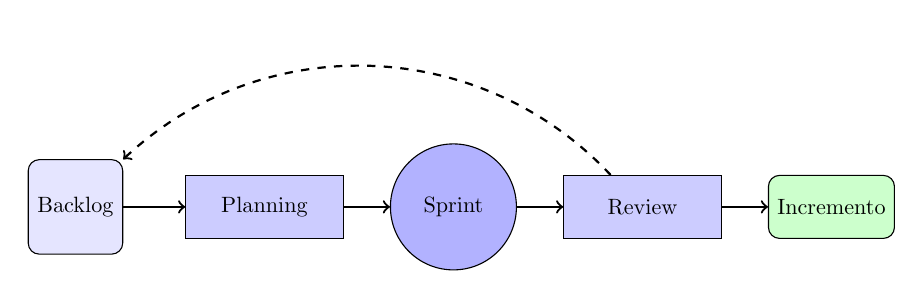
\begin{tikzpicture}[node distance=2.5cm, auto, scale=0.8, transform shape]
    \node (backlog) [draw, rectangle, rounded corners, minimum height=1.5cm, minimum width=1.5cm, fill=blue!10] {Backlog};
    \node (sprintplan) [draw, rectangle, minimum width=2.5cm, minimum height=1cm, fill=blue!20, right of=backlog, node distance=3cm] {Planning};
    \node (sprint) [draw, circle, minimum size=2cm, fill=blue!30, right of=sprintplan, node distance=3cm] {Sprint};
    \node (review) [draw, rectangle, minimum width=2.5cm, minimum height=1cm, fill=blue!20, right of=sprint, node distance=3cm] {Review};
    \node (inc) [draw, rectangle, rounded corners, minimum width=2cm, minimum height=1cm, fill=green!20, right of=review, node distance=3cm] {Incremento};

    \draw[->, thick] (backlog) -- (sprintplan);
    \draw[->, thick] (sprintplan) -- (sprint);
    \draw[->, thick] (sprint) -- (review);
    \draw[->, thick] (review) -- (inc);
    \draw[->, thick, dashed] (review) to[bend right=45] (backlog);
\end{tikzpicture}
\captionof{figure}{Ciclo de Vida de Scrum}
\end{center}
\vspace{0.5cm}
\newpage
\subsubsection{Kanban}
\textbf{Enfoque:} Está basado en los principios Lean y se centra en hacer visible el flujo de trabajo y en entregar de forma continua. En vez de usar Sprints de duración fija, regula el ritmo limitando la cantidad de tareas que pueden estar en curso al mismo tiempo, lo que se conoce como límite de trabajo en progreso o WIP (Work in Progress) \citep{anderson2010kanban}.

\textbf{Fases o Prácticas Principales:}
\begin{enumerate}
    \item Visualización del flujo: Se dibuja el proceso en columnas (por ejemplo, Por Hacer, En Desarrollo, Pruebas y Hecho).
    \item Límites de WIP: Se fija un máximo de tareas por columna.
    \item Control del flujo: Se revisa el avance para resolver rápido los bloqueos.
    \item Mejora continua: El proceso se va ajustando con el tiempo.
\end{enumerate}

\textbf{Representación Gráfica:}
\vspace{0.5cm}
\begin{center}
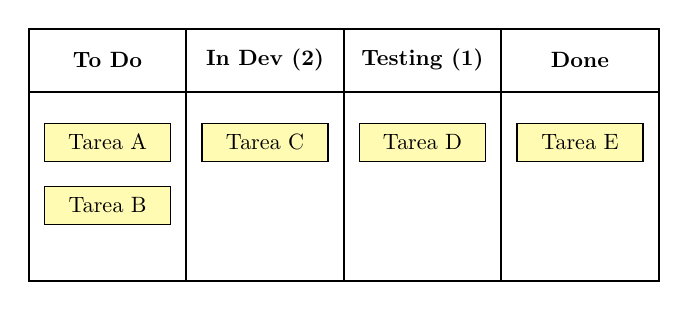
\begin{tikzpicture}[scale=0.8, transform shape]
    % Tablero
    \draw[thick] (0,0) rectangle (10,4);
    \draw[thick] (2.5,0) -- (2.5,4);
    \draw[thick] (5,0) -- (5,4);
    \draw[thick] (7.5,0) -- (7.5,4);

    % Cabeceras
    \node at (1.25, 3.5) {\textbf{To Do}};
    \node at (3.75, 3.5) {\textbf{In Dev (2)}};
    \node at (6.25, 3.5) {\textbf{Testing (1)}};
    \node at (8.75, 3.5) {\textbf{Done}};
    \draw[thick] (0,3) -- (10,3);

    % Tarjetas
    \node[draw, fill=yellow!30, minimum width=2cm, minimum height=0.6cm] at (1.25, 2.2) {Tarea A};
    \node[draw, fill=yellow!30, minimum width=2cm, minimum height=0.6cm] at (1.25, 1.2) {Tarea B};
    \node[draw, fill=yellow!30, minimum width=2cm, minimum height=0.6cm] at (3.75, 2.2) {Tarea C};
    \node[draw, fill=yellow!30, minimum width=2cm, minimum height=0.6cm] at (6.25, 2.2) {Tarea D};
    \node[draw, fill=yellow!30, minimum width=2cm, minimum height=0.6cm] at (8.75, 2.2) {Tarea E};
\end{tikzpicture}
\captionof{figure}{Tablero Kanban Básico}
\end{center}
\vspace{0.5cm}
\newpage
\subsubsection{Prototipo Evolutivo}
\textbf{Enfoque:} Es un modelo en el que se construye rápidamente una primera versión funcional del sistema, que se muestra al usuario y se va mejorando en versiones sucesivas hasta convertirse en el producto final. A diferencia del prototipo desechable, que solo sirve para aclarar requisitos y después se descarta, en el prototipo evolutivo el código no se bota, sino que cada versión parte de la anterior. Es útil cuando los requisitos no están del todo claros al inicio y se necesita ver algo funcionando para definirlos mejor \citep{sommerville2015, pressman2010}.

\textbf{Fases o Etapas:}
\begin{enumerate}
    \item Comunicación: Se identifican con los usuarios los requisitos generales que ya se conocen.
    \item Diseño rápido: Se diseña de forma simple lo que el usuario va a ver, como las pantallas y el flujo principal.
    \item Construcción del prototipo: Se programa una versión funcional con las partes más importantes.
    \item Evaluación: El usuario prueba el prototipo y entrega sus comentarios.
    \item Refinamiento: Con esos comentarios se mejora el prototipo y se vuelve a evaluar, hasta llegar al producto final.
\end{enumerate}

\textbf{Representación Gráfica:}
\vspace{0.5cm}
\begin{center}
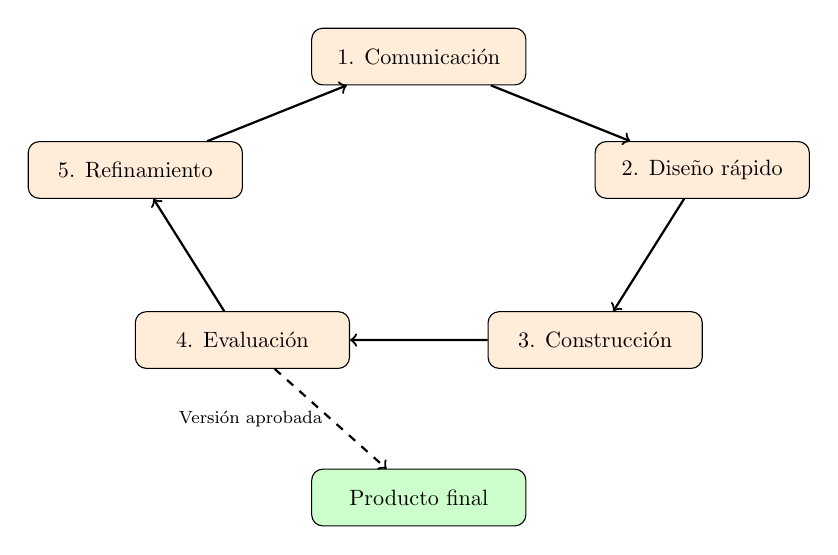
\begin{tikzpicture}[scale=0.8, transform shape,
    box/.style={draw, rectangle, rounded corners, minimum width=3.4cm, minimum height=0.9cm, fill=orange!15, text centered}]
    \node (com) [box] at (0,3) {1. Comunicación};
    \node (dis) [box] at (4.5,1.2) {2. Diseño rápido};
    \node (con) [box] at (2.8,-1.5) {3. Construcción};
    \node (eva) [box] at (-2.8,-1.5) {4. Evaluación};
    \node (ref) [box] at (-4.5,1.2) {5. Refinamiento};
    \node (fin) [draw, rectangle, rounded corners, minimum width=3.4cm, minimum height=0.9cm, fill=green!20] at (0,-4) {Producto final};

    \draw[->, thick] (com) -- (dis);
    \draw[->, thick] (dis) -- (con);
    \draw[->, thick] (con) -- (eva);
    \draw[->, thick] (eva) -- (ref);
    \draw[->, thick] (ref) -- (com);
    \draw[->, thick, dashed] (eva) -- node[left, font=\footnotesize] {Versión aprobada} (fin);
\end{tikzpicture}
\captionof{figure}{Ciclo del Prototipo Evolutivo}
\end{center}
\vspace{0.5cm}
\newpage
\subsection{Evaluación de Alternativas}
Para elegir la metodología más adecuada, los tres enfoques se evaluaron según los siguientes criterios:

\begin{itemize}
    \item \textbf{Aplicabilidad:} Qué tan bien se adapta a proyectos con mucha innovación, integración de APIs y modelos de cálculo.
    \item \textbf{Eficiencia:} Qué tan rápido permite tener entregables y versiones funcionales.
    \item \textbf{Costo y riesgos:} Qué tan fácil es reducir riesgos o cambiar de rumbo sin un gran costo.
    \item \textbf{Calidad:} Qué tanto favorece la validación constante, las pruebas y la retroalimentación.
    \item \textbf{Adaptabilidad:} Qué tan flexible es para incorporar cambios en los requisitos en etapas avanzadas.
    \item \textbf{Ajuste a un solo desarrollador:} Qué tan bien funciona cuando todo el trabajo lo hace una sola persona.
    \item \textbf{Carga de documentación:} Cuánto trabajo exige documentar el proceso, como reuniones, tableros y registros de avance.
    \item \textbf{Ajuste al plazo del MVP:} Qué tanto ayuda a llegar a un producto mínimo viable antes de diciembre de 2026.
\end{itemize}
\newpage
\subsection{Cuadro Comparativo}
\begin{table}[h!]
    \centering
    \renewcommand{\arraystretch}{1.4}
    \begin{tabular}{|m{2.9cm}|m{3.8cm}|m{3.8cm}|m{3.8cm}|}
        \hline
        \rowcolor[HTML]{EFEFEF}
        \textbf{Criterio} & \textbf{Scrum (Ágil)} & \textbf{Kanban (Lean/Ágil)} & \textbf{Prototipo evolutivo} \\ \hline
        \textbf{Aplicabilidad} & Alta. Permite probar las integraciones en ciclos cortos. & Alta. El flujo continuo permite incorporar cambios día a día. & Alta. Sirve cuando los requisitos no están claros, como en el cálculo de la fatiga cruzada. \\ \hline
        \textbf{Eficiencia} & Alta. Entrega partes funcionales al final de cada Sprint. & Media-Alta. Entrega continua, enfocada en evitar atascos. & Alta. Desde temprano hay una versión que se puede usar y probar. \\ \hline
        \textbf{Costo y riesgos} & Bajo riesgo. Los errores se detectan en las primeras iteraciones. & Bajo riesgo. Los bloqueos se ven de inmediato. & Riesgo medio. Detecta temprano errores en los requisitos, pero el código puede crecer desordenado si no se revisa. \\ \hline
        \textbf{Calidad} & Validación constante en cada Sprint Review. & Alta, gracias al límite de trabajo en curso (WIP). & Retroalimentación constante del usuario, aunque la estructura interna puede deteriorarse. \\ \hline
        \textbf{Adaptabilidad} & Alta. Los requerimientos se pueden ajustar entre Sprints. & Muy alta. Las prioridades cambian según se necesite. & Muy alta. Cada nueva versión incorpora los cambios. \\ \hline
        \textbf{Un solo desarrollador} & Baja. Sus roles y reuniones están pensados para equipos. & Alta. Funciona igual con una sola persona. & Alta. No exige roles ni reuniones fijas. \\ \hline
        \textbf{Carga de documentación} & Alta. Hay que registrar el Product Backlog, la planificación, la revisión y la retrospectiva de cada Sprint. & Media-Alta. Hay que mantener al día el tablero, los límites de trabajo y el registro del flujo. & Baja. Se documenta cada versión del prototipo y el resultado de su evaluación. \\ \hline
        \textbf{Ajuste al plazo del MVP} & Media. Ordena el avance, pero sus reuniones restan tiempo de desarrollo. & Media. Ayuda a terminar tareas, pero no define cuándo se entrega una versión. & Alta. Cada versión acerca la aplicación al MVP final. \\ \hline
    \end{tabular}
    \caption{Cuadro comparativo de alternativas metodológicas.}
    \label{tab:comparativa_metodologias}
\end{table}
\newpage
\subsection{Justificación Metodología Seleccionada}

Después de evaluar las alternativas, se eligió el \textbf{modelo de prototipo evolutivo} como metodología de desarrollo del proyecto. Scrum y Kanban fueron analizadas porque son metodologías muy usadas y con buenos resultados, pero se descartaron por las siguientes razones:
\begin{itemize}
    \item \textbf{Scrum:} Está pensado para equipos, con roles y reuniones que no tienen mucho sentido cuando el desarrollo lo hace una sola persona. Además, exige documentar todo el proceso (Product Backlog, planificación, revisión y retrospectiva de cada Sprint), lo que le quita tiempo al desarrollo.
    \item \textbf{Kanban:} Ordena muy bien el trabajo diario, pero también requiere mantener al día el tablero y el registro del flujo. Además, por sí solo no define en qué momento se entrega una versión funcional para evaluarla.
\end{itemize}

El prototipo evolutivo, en cambio, se ajusta mejor a este proyecto por cuatro motivos:
\begin{itemize}
    \item \textbf{Los requisitos se aclaran con el uso:} El cálculo de la fatiga cruzada y las sugerencias de nutrición necesitan probarse para saber si funcionan bien. Con un prototipo funcional se pueden ajustar a partir de lo que se observa en cada evaluación.
    \item \textbf{Menos documentación de proceso:} Solo se documenta cada versión y su evaluación, lo que es más realista para una sola persona que además debe cumplir con los plazos académicos.
    \item \textbf{Lleva directo al MVP:} El código no se bota. Cada versión parte de la anterior, por lo que la última versión del prototipo es el producto mínimo viable que plantea el objetivo general.
    \item \textbf{Permite probar temprano si la aplicación es fácil de usar:} Uno de los problemas identificados en el Capítulo 2 es lo engorroso que resulta usar las aplicaciones actuales. Con un prototipo se puede comprobar desde el inicio si la aplicación es simple de usar.
\end{itemize}

Para controlar el principal riesgo de este modelo, que es que el código crezca de forma desordenada, al final de cada versión se reservará tiempo para ordenar el código, y el backend se organizará en módulos independientes desde el comienzo.
\newpage
\subsection{Diseño del Plan Metodológico del Proyecto}

El desarrollo se organiza en versiones sucesivas del prototipo, de 2 a 3 semanas cada una. Cada versión pasa por las cinco fases del modelo:

\begin{enumerate}
    \item \textbf{Fase 1: Comunicación:}
    Se definen los requisitos que se abordarán en la versión, a partir de los requerimientos del sistema y de los resultados de la versión anterior.

    \item \textbf{Fase 2: Diseño rápido:}
    Se diseñan las pantallas y el flujo de las funciones nuevas, junto con los cambios necesarios en la base de datos y en los servicios del backend.

    \item \textbf{Fase 3: Construcción del prototipo:}
    Se programan las funciones de la versión sobre el prototipo existente. Para no dispersar el trabajo, se aborda un componente pesado a la vez, por ejemplo el módulo de cardio o el procesamiento de lenguaje natural.

    \item \textbf{Fase 4: Evaluación:}
    Se hacen pruebas técnicas, por ejemplo simulando datos de un wearable o verificando que las metas nutricionales se ajusten bien al gasto registrado. También se prueba el prototipo con usuarios para recoger sus comentarios.

    \item \textbf{Fase 5: Refinamiento:}
    Con los resultados de la evaluación se corrigen errores, se ordena el código y se definen los ajustes para la siguiente versión. Cuando una versión cumple con todos los requerimientos del MVP, se cierra el ciclo.
\end{enumerate}

Las versiones del prototipo se planifican de la siguiente forma:

\begin{center}
    \renewcommand{\arraystretch}{1.4}
    \begin{tabular}{|>{\raggedright\arraybackslash}m{3.0cm}|m{11.9cm}|}
        \hline
        \rowcolor[HTML]{EFEFEF}
        \textbf{Versión} & \textbf{Contenido principal} \\ \hline
        \textbf{Versión 1} & Creación de la cuenta con los términos de uso y el aviso legal, cuestionario inicial del perfil del usuario y registro manual de entrenamientos de fuerza y de comidas, con los catálogos de ejercicios y alimentos, incluida la lectura de códigos de barras. \\ \hline
        \textbf{Versión 2} & Registro de entrenamientos de resistencia con el GPS del teléfono y lectura automática desde Health Connect y Apple Health. \\ \hline
        \textbf{Versión 3} & Registro asistido por inteligencia artificial (lenguaje natural y fotos de comida) y carga de archivos \texttt{.fit}. \\ \hline
        \textbf{Versión 4} & Cruce de datos: cálculo de fatiga, alertas, metas de alimentación según el entrenamiento, línea de tiempo del progreso y plan semanal sugerido según el perfil. \\ \hline
        \rowcolor[HTML]{E8F5E9}
        \textbf{Versión 5 (MVP)} & Red social básica (seguir usuarios, publicar sesiones, rutas y comidas con fotos en el perfil y agregarlas a los propios módulos), panel de administración, control de datos personales y suscripción al plan premium. Con esta versión se completa el MVP. \\ \hline
        \textbf{Después del MVP} & Récords de tramo, récords de fuerza comparados, retos entre seguidores y videos en las publicaciones. \\ \hline
    \end{tabular}
    \captionof{table}{Planificación de las versiones del prototipo evolutivo.}
    \label{tab:versiones_prototipo}
\end{center}

Hay que distinguir entre el prototipo de demostración y el MVP. El prototipo que se usa hoy en las pruebas deja fuera la subida de fotos, para ahorrar costos de almacenamiento mientras se desarrolla. El MVP, en cambio, sí permite publicar fotos, porque es la primera versión que llegará a usuarios reales y lo visual es uno de los mayores atractivos de una red social. Por eso las fotos se suman en la versión 5, junto con el resto de la red social.

\vspace{0.5cm}
\begin{center}
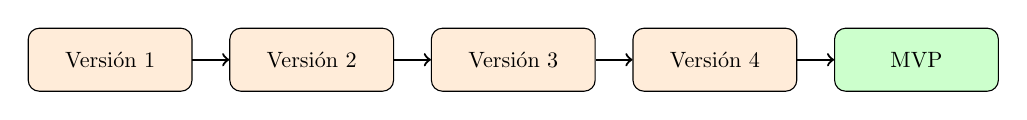
\begin{tikzpicture}[node distance=3.2cm, scale=0.8, transform shape,
    box/.style={draw, rectangle, rounded corners, minimum width=2.6cm, minimum height=1cm, fill=orange!15, text centered}]
    \node (v1) [box] {Versión 1};
    \node (v2) [box, right of=v1] {Versión 2};
    \node (v3) [box, right of=v2] {Versión 3};
    \node (v4) [box, right of=v3] {Versión 4};
    \node (v5) [box, right of=v4, fill=green!20] {MVP};
    \draw[->, thick] (v1) -- (v2);
    \draw[->, thick] (v2) -- (v3);
    \draw[->, thick] (v3) -- (v4);
    \draw[->, thick] (v4) -- (v5);
\end{tikzpicture}
\captionof{figure}{Evolución del prototipo hasta el MVP}
\end{center}

\subsection{Comentarios Generales del Capítulo}

En resumen, definir la metodología permite ordenar el trabajo y reducir la incertidumbre propia de este proyecto. Se analizaron Scrum, Kanban y el prototipo evolutivo, y se eligió este último. Scrum y Kanban se descartaron porque exigen documentar y mantener todo el proceso, algo poco práctico para una sola persona con un plazo acotado. El prototipo evolutivo, en cambio, permite tener una versión funcional desde temprano, ajustar los requisitos con lo que se aprende en cada evaluación y llegar al MVP con la última versión. Con esta base, en el siguiente capítulo se presentan las alternativas de solución y los estudios de factibilidad técnica, económica y operativa.
\newpage

% Alternativas de Solución
% Este archivo se incluye desde main.tex con \input.
\section{Alternativas de Solución}
\subsection{Introducción del Capítulo}
Una vez definida la metodología, en este capítulo se presentan las distintas alternativas de arquitectura y funcionalidades que se evaluaron para construir la solución. Cada alternativa tiene un nivel de complejidad distinto. La diferencia principal está en cómo se obtienen los datos cardiovasculares, que es la parte más variable desde el punto de vista técnico, pero también cambian el registro de nutrición, el uso de inteligencia artificial y el nivel de detalle del cruce de datos.
\\\\
Las tres alternativas comparten la misma base tecnológica y el mismo motor de cruce de datos, que funciona ordenando los eventos en el tiempo. Lo que cambia entre ellas es la cantidad y la calidad de los datos que recibe ese motor, y eso influye directamente en qué tan precisas son sus estimaciones de fatiga cruzada.
\subsection{Descripción de Alternativas}
\subsubsection{Base Tecnológica Común}

Sea cual sea la alternativa elegida, la solución se construirá con las siguientes tecnologías:

\begin{itemize}
    \item \textbf{Frontend Móvil:} Flutter (Dart), un framework multiplataforma que permite crear aplicaciones para Android e iOS con un solo código, lo que reduce el tiempo de desarrollo y mantenimiento.
    \item \textbf{Backend / API:} NestJS (Node.js con TypeScript), un framework para construir aplicaciones del lado del servidor. Su estructura por módulos facilita que el sistema crezca y que cada parte (nutrición, fuerza, cardio y analítica) quede separada.
    \newpage
    \item \textbf{Base de Datos:} MongoDB, una base de datos NoSQL orientada a documentos. Cada registro se guarda como un documento en formato BSON, sin necesidad de una estructura fija. Las sesiones de entrenamiento, las comidas y los datos de los dispositivos se guardan como documentos que se pueden consultar con índices aunque su estructura cambie (por ejemplo, una sesión de fuerza con 4 ejercicios y otra con 7).
    \item \textbf{Almacenamiento de Imágenes y Archivos:} Amazon S3, un servicio de almacenamiento de objetos, junto con Amazon CloudFront, una red de distribución de contenido (CDN) que guarda copias de las imágenes en servidores cercanos a los usuarios para que carguen rápido. Las fotos no se guardan dentro de MongoDB, porque harían crecer mucho la base de datos y sus respaldos. En la base de datos solo queda la dirección de cada archivo.
\end{itemize}

\textbf{Motor de Cruce de Datos Basado en Timestamps}

Lo que más diferencia a esta plataforma es que cruza los datos de fuerza, resistencia y nutrición para estimar la fatiga cruzada. El motor funciona ordenando todo en el tiempo. Cada evento registrado (una comida, una sesión de fuerza, una sesión de cardio o un reporte de sensaciones) se guarda con su fecha y hora exacta (timestamp). A partir de esa información, el motor calcula lo siguiente:

\begin{enumerate}
    \item \textbf{Ventanas de recuperación:} El tiempo que pasa entre el fin de una sesión de fuerza y el inicio de la siguiente sesión de cardio, y al revés. Compara ese tiempo con lo que recomienda la literatura (al menos 6 a 8 horas entre sesiones de distinto tipo) para avisar cuando hay riesgo de interferencia.
    \item \textbf{Horario de las comidas:} Revisa si las comidas se hicieron en los momentos recomendados respecto al entrenamiento. Por ejemplo, carbohidratos 2 a 3 horas antes del cardio, proteínas dentro de las 2 horas posteriores a la fuerza, o si se comió en el momento adecuado durante una ruta larga.
    \item \textbf{Fatiga acumulada semanal:} Suma el volumen de entrenamiento de los últimos 7 días. En fuerza se calcula como $\sum(\text{series} \times \text{repeticiones} \times \text{peso})$. En cardio, la medida depende de la alternativa, y va desde distancia $\times$ RPE en la más básica hasta una carga basada en zonas cardíacas y potencia en las más avanzadas.
    \item \textbf{Detección de interferencia:} Si en días seguidos hay secuencias de fuerza $\rightarrow$ cardio (o al revés) con poca recuperación entre ellas, el sistema muestra una alerta y sugiere reorganizar el calendario.
\end{enumerate}

La lógica del motor es \textbf{la misma} en las tres alternativas. Lo que cambia es la \textbf{calidad y el nivel de detalle de los datos que recibe}. Mientras más información tenga (frecuencia cardíaca, potencia, cadencia), más precisas serán sus estimaciones.

\textbf{Almacenamiento de Imágenes}

Las tres alternativas guardan fotos, aunque en cantidades muy distintas. La Alternativa 1 solo guarda la foto de perfil, la Alternativa 2 agrega una foto por receta compartida y la Alternativa 3 permite hasta 4 fotos por publicación en la red social. Para que las fotos no encarezcan ni hagan más lenta la aplicación, las tres siguen el mismo esquema:

\begin{enumerate}
    \item El teléfono reduce la foto a un máximo de 1080 píxeles por lado y la comprime, dejándola en unos 300 KB. También crea una miniatura de unos 40 KB para mostrarla en el muro y le borra los datos de ubicación (EXIF).
    \item La aplicación le pide al backend un permiso de subida que dura pocos minutos (URL prefirmada). Con ese permiso, el teléfono sube la foto directamente a Amazon S3, sin pasar por el servidor de NestJS, que así no tiene que recibir archivos pesados.
    \item El backend guarda en MongoDB solo la dirección de la foto, dentro del documento al que pertenece (por ejemplo, la publicación o el perfil).
    \item Para mostrar las fotos, la aplicación las pide a Amazon CloudFront, que las mantiene en caché. El bucket de S3 es privado y solo CloudFront puede leerlo.
    \item Una regla automática del bucket borra las fotos que se subieron pero nunca se publicaron, y las de publicaciones o cuentas eliminadas.
\end{enumerate}

Las fotos que se sacan solo para registrar una comida con IA no pasan por S3. El backend las envía al servicio de IA y las descarta después del análisis, salvo que el usuario decida publicarlas.
\\\\
También se evaluaron otras opciones. Guardar las fotos dentro de MongoDB (con GridFS) haría crecer la base de datos administrada, que cobra más por cada GB que S3, y volvería más lentos los respaldos. Servicios como Firebase Storage o Cloudflare R2 también servirían, pero sumarían otro proveedor. Como el resto de la infraestructura ya está en AWS y el nivel gratuito de CloudFront cubre la entrega de las fotos, se eligió S3 con CloudFront. El costo de este esquema se calcula en la factibilidad económica (Tabla \ref{tab:costo_imagenes}).

\subsubsection{Alternativa 1: Solución Minimalista (MVP Lean)}

\textbf{Descripción General}

Esta alternativa es la versión más simple que todavía permite abordar el problema del entrenamiento concurrente. Busca reducir el costo y el tiempo de desarrollo, a cambio de tener menos automatización y datos menos precisos. Está pensada para usuarios que no tienen wearables y que están dispuestos a registrar su actividad a mano.
\\\\
\textbf{Módulo de Nutrición}

Las comidas se registran solo con formularios. El usuario elige los ingredientes desde una base de datos alimentada por una API gratuita de alimentos (como OpenFoodFacts) e ingresa las cantidades. El sistema calcula automáticamente los macronutrientes y las calorías de cada comida. No se usa inteligencia artificial para estimar la comida a partir de fotos ni de texto libre.
\\\\
\textbf{Módulo de Fuerza}

El usuario crea rutinas base (plantillas de ejercicios) y registra cada sesión con un formulario, eligiendo el ejercicio e ingresando series, repeticiones y peso. Incluye un campo de texto libre para anotar las sensaciones de cada ejercicio. No se incluye registro por lenguaje natural.
\newpage
\textbf{Módulo de Cardio}

El registro de cardio usa solo el GPS del teléfono y la percepción del esfuerzo (RPE). La aplicación graba la ruta, la velocidad, la distancia y el tiempo con la ubicación del teléfono. Al terminar la sesión, el usuario indica su RPE en una escala de 1 a 10 y puede agregar notas. No hay integración con wearables, Health Connect, Apple Health ni archivos \texttt{.fit}.
\\\\
\textbf{Motor de Cruce de Datos}

En este caso el motor de cruce trabaja con pocos datos. La fatiga del cardio se estima a partir de la distancia, el tiempo y el RPE. Como no hay datos de frecuencia cardíaca, no se pueden calcular las zonas de entrenamiento ni el gasto real de calorías, así que las estimaciones de fatiga cruzada son aproximaciones basadas en lo que el usuario declara.
\\\\
\textbf{Módulo Social}

Incluye una comunidad básica donde los usuarios pueden compartir rutas, rutinas de fuerza y recetas. No incluye el ajuste automático de porciones. Las publicaciones no llevan fotos, así que las únicas imágenes que guarda esta alternativa son las fotos de perfil.
\\\\
\textbf{Arquitectura de la Solución}

La arquitectura de esta alternativa es monolítica y sencilla. La aplicación móvil (Flutter) se comunica con una API REST hecha en NestJS, que contiene toda la lógica de negocio y guarda los datos en MongoDB. Las fotos de perfil se suben directamente desde el teléfono a Amazon S3 y se muestran a través de CloudFront.

\vspace{0.5cm}
\begin{center}
\setstretch{1}
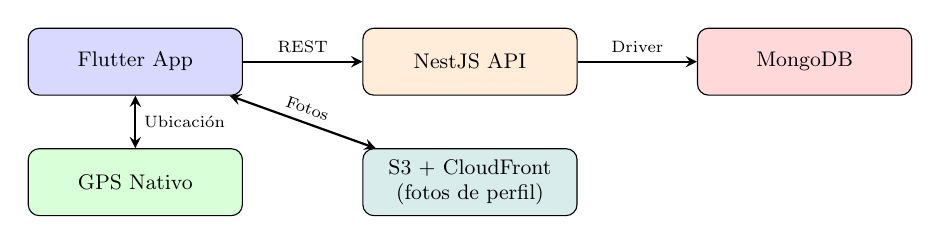
\begin{tikzpicture}[
    node distance=1.8cm,
    box/.style={draw, rectangle, rounded corners, minimum width=3.2cm, minimum height=1cm, fill=#1, text centered, font=\small},
    arrow/.style={->, thick, >=stealth},
    scale=0.85, transform shape
]
    % Frontend
    \node (app) [box=blue!15] {Flutter App};
    \node (gps) [box=green!15, below of=app] {GPS Nativo};

    % Backend
    \node (api) [box=orange!15, right of=app, node distance=5cm] {NestJS API};

    % Database
    \node (db) [box=red!15, right of=api, node distance=5cm] {MongoDB};

    % Arrows
    \draw[arrow] (app) -- node[above, font=\scriptsize] {REST} (api);
    \draw[arrow] (api) -- node[above, font=\scriptsize] {Driver} (db);
    \draw[arrow, <->] (app) -- node[right, font=\scriptsize] {Ubicación} (gps);

    % Fotos
    \node (s3) [box=teal!15, below of=api] {\shortstack{S3 + CloudFront\\(fotos de perfil)}};
    \draw[arrow, <->] (app) -- node[above, sloped, font=\scriptsize] {Fotos} (s3);

\end{tikzpicture}
\captionof{figure}{Arquitectura de la Alternativa 1: Solución Minimalista.}
\end{center}
\vspace{0.5cm}
\newpage
\textbf{Estimación de Costos}

La siguiente tabla resume los costos de esta alternativa. El costo de desarrollo viene del análisis por ciclo de vida (Tabla \ref{tab:ciclovida_alt1}), y los demás valores son los mismos que se usan en su flujo de caja dentro de la factibilidad económica.

\begin{table}[h!]
    \centering
    \renewcommand{\arraystretch}{1.4}
    \begin{tabular}{|m{4cm}|m{5.5cm}|r|}
        \hline
        \rowcolor[HTML]{EFEFEF}
        \textbf{Ítem} & \textbf{Detalle} & \textbf{Costo (CLP)} \\ \hline
        \multicolumn{3}{|l|}{\cellcolor[HTML]{E3F2FD}\textbf{Inversión inicial (Año 0)}} \\ \hline
        Desarrollo de software & 260 horas de trabajo según el ciclo de vida & \$8.545.627 \\ \hline
        Publicación en tiendas & Google Play y Apple Developer & \$120.602 \\ \hline
        \rowcolor[HTML]{E8F5E9}
        \textbf{Total inversión inicial} & & \textbf{\$8.666.229} \\ \hline
        \multicolumn{3}{|l|}{\cellcolor[HTML]{FFF3E0}\textbf{Costos operativos anuales (Años 1 a 4)}} \\ \hline
        Infraestructura Cloud & AWS (Fargate, ALB, IP públicas y CloudWatch) y MongoDB Atlas M10 (Tabla \ref{tab:costo_infra}) & \$1.879.063 \\ \hline
        Imágenes & S3 y CloudFront para las fotos de perfil (Tabla \ref{tab:costo_imagenes}) & \$11.671 \\ \hline
        APIs de IA & No utiliza IA & No aplica \\ \hline
        Mantenimiento & 10\% del costo de desarrollo & \$854.563 \\ \hline
        Suscripción Apple & Renovación anual del Apple Developer Program & \$96.287 \\ \hline
        \rowcolor[HTML]{FFF3E0}
        \textbf{Total operativo anual} & & \textbf{\$2.841.584} \\ \hline
    \end{tabular}
    \caption{Estimación de costos de la Alternativa 1: Solución Minimalista.}
    \label{tab:costos_alt1}
\end{table}

\newpage
\subsubsection{Alternativa 2: Solución Integrada con Brokers del Sistema Operativo}

\textbf{Descripción General}

Esta alternativa sigue lo que hoy hace la mayoría de las aplicaciones deportivas. Deja que los wearables del usuario registren los datos más pesados y los lee de forma automática desde los concentradores del sistema operativo, que son \textbf{Health Connect} en Android y \textbf{Apple Health (HealthKit)} en iOS. Además, usa inteligencia artificial para que registrar comidas y rutinas de fuerza sea más rápido.
\\\\
\textbf{Módulo de Nutrición}

Las comidas se pueden registrar de dos formas con ayuda de inteligencia artificial:
\begin{itemize}
    \item \textbf{Procesamiento de Lenguaje Natural (PLN):} El usuario describe su comida con sus propias palabras (por ejemplo, ``desayuné 3 huevos con avena y yogurt'') y el sistema separa los ingredientes y estima los macronutrientes.
    \item \textbf{Visión Artificial:} El usuario saca una foto a su plato y un modelo estima qué alimentos hay y en qué cantidad. Después, el usuario puede corregir el resultado.
\end{itemize}
Ambas funciones usan una API de inteligencia artificial en la nube (Gemini, con sus modelos Flash). La base de datos de alimentos se mantiene para validar y corregir los resultados.
\\\\
\textbf{Módulo de Fuerza}

Además del formulario, se agrega el registro por lenguaje natural. El usuario puede dictar o escribir su rutina (por ejemplo, ``hice 3 series de 10 sentadillas con 80 kilos'') y el sistema identifica el ejercicio, las series, las repeticiones y el peso, y los guarda en la base de datos. También se mantiene el registro de sensaciones de cada ejercicio.
\newpage
\textbf{Módulo de Cardio}

El sistema lee automáticamente los datos que reúnen Health Connect (Android) y Apple Health (iOS). Cuando el usuario termina una sesión de cardio registrada con un wearable compatible (Garmin, Polar, Apple Watch, Samsung Galaxy Watch, entre otros), los datos se sincronizan con el concentrador del teléfono y la aplicación los importa en segundo plano. Los datos disponibles a través de estos concentradores son:

\begin{itemize}
    \item Frecuencia cardíaca promedio y máxima de la sesión.
    \item Calorías activas estimadas por el dispositivo.
    \item Distancia recorrida y duración.
    \item Ruta GPS (cuando el wearable la registra).
    \item Zonas de ritmo cardíaco (calculadas por la aplicación a partir de la FC importada).
\end{itemize}

Además, se mantiene el GPS del teléfono como respaldo para usuarios sin wearable, junto con el RPE.
\\\\
\textbf{Motor de Cruce de Datos}

Al contar con la frecuencia cardíaca y las calorías activas reales, el motor de cruce es más preciso. Puede calcular las zonas de entrenamiento (Zona 1 a Zona 5) y separar el gasto calórico según el tipo de esfuerzo. Con eso, el módulo de nutrición puede ajustar los macronutrientes según la fuente de energía que más se usó (carbohidratos en zonas altas y grasas en zonas bajas). Las estimaciones de fatiga cruzada también mejoran, porque consideran la carga interna (el esfuerzo del corazón) y no solo la carga externa (volumen y distancia).
\\\\
\textbf{Módulo Social}

Incluye la comunidad para compartir rutas, rutinas y recetas, y agrega el ajuste automático de porciones. El sistema toma una receta de la comunidad y ajusta las cantidades de cada ingrediente para cubrir los macronutrientes que el usuario necesita según el desgaste del día. Cada receta compartida puede llevar una foto del plato, además de la foto de perfil de cada usuario.
\newpage
\textbf{Arquitectura de la Solución}

La arquitectura agrega la conexión con los SDKs de Health Connect y HealthKit, además de un servicio de inteligencia artificial en la nube para el procesamiento de lenguaje natural y la visión artificial. Las fotos de perfil y de las recetas se guardan en Amazon S3 y se muestran a través de CloudFront.

\vspace{0.5cm}
\begin{center}
\setstretch{1}
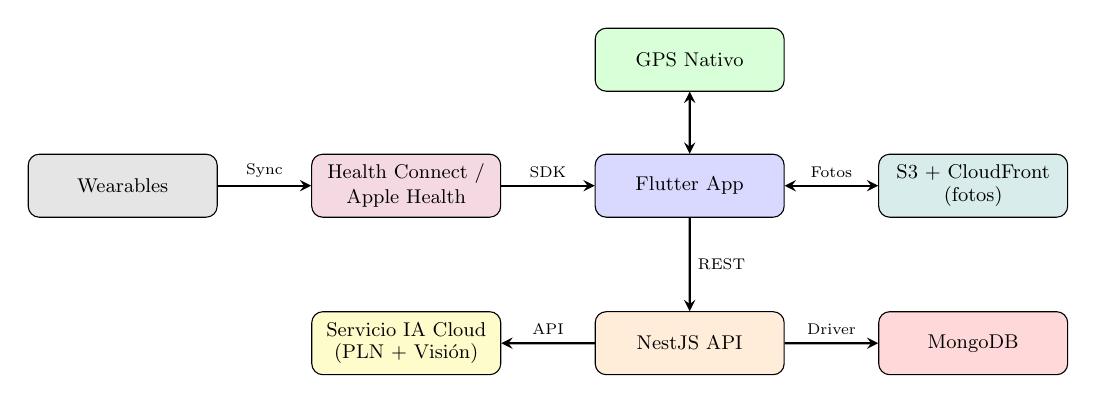
\begin{tikzpicture}[
    node distance=2cm,
    box/.style={draw, rectangle, rounded corners, minimum width=3cm, minimum height=1cm, fill=#1, text centered, font=\small},
    arrow/.style={->, thick, >=stealth},
    darrow/.style={<->, thick, >=stealth},
    scale=0.8, transform shape
]
    % External devices
    \node (wear) [box=gray!20] {Wearables};
    \node (hc) [box=purple!15, right of=wear, node distance=4.5cm] {\shortstack{Health Connect /\\Apple Health}};

    % Frontend
    \node (app) [box=blue!15, right of=hc, node distance=4.5cm] {Flutter App};

    % Backend
    \node (api) [box=orange!15, below of=app, node distance=2.5cm] {NestJS API};

    % AI Service
    \node (ai) [box=yellow!20, left of=api, node distance=4.5cm] {\shortstack{Servicio IA Cloud\\(PLN + Visión)}};

    % Database
    \node (db) [box=red!15, right of=api, node distance=4.5cm] {MongoDB};

    % GPS
    \node (gps) [box=green!15, above of=app, node distance=2cm] {GPS Nativo};

    % Arrows
    \draw[arrow] (wear) -- node[above, font=\scriptsize] {Sync} (hc);
    \draw[arrow] (hc) -- node[above, font=\scriptsize] {SDK} (app);
    \draw[arrow] (app) -- node[right, font=\scriptsize] {REST} (api);
    \draw[arrow] (api) -- node[above, font=\scriptsize] {Driver} (db);
    \draw[arrow] (api) -- node[above, font=\scriptsize] {API} (ai);
    \draw[darrow] (gps) -- node[right, font=\scriptsize] {} (app);

    % Fotos
    \node (s3) [box=teal!15, right of=app, node distance=4.5cm] {\shortstack{S3 + CloudFront\\(fotos)}};
    \draw[darrow] (app) -- node[above, font=\scriptsize] {Fotos} (s3);

\end{tikzpicture}
\captionof{figure}{Arquitectura de la Alternativa 2: Solución Integrada con Brokers del SO.}
\end{center}
\vspace{0.5cm}
\newpage
\textbf{Estimación de Costos}

La siguiente tabla resume los costos de esta alternativa. El costo de desarrollo viene del análisis por ciclo de vida (Tabla \ref{tab:ciclovida_alt2}), y los demás valores son los mismos que se usan en su flujo de caja dentro de la factibilidad económica.

\begin{table}[h!]
    \centering
    \renewcommand{\arraystretch}{1.4}
    \begin{tabular}{|m{4cm}|m{5.5cm}|r|}
        \hline
        \rowcolor[HTML]{EFEFEF}
        \textbf{Ítem} & \textbf{Detalle} & \textbf{Costo (CLP)} \\ \hline
        \multicolumn{3}{|l|}{\cellcolor[HTML]{E3F2FD}\textbf{Inversión inicial (Año 0)}} \\ \hline
        Desarrollo de software & 385 horas de trabajo según el ciclo de vida & \$12.122.388 \\ \hline
        Publicación en tiendas & Google Play y Apple Developer & \$120.602 \\ \hline
        \rowcolor[HTML]{E8F5E9}
        \textbf{Total inversión inicial} & & \textbf{\$12.242.990} \\ \hline
        \multicolumn{3}{|l|}{\cellcolor[HTML]{FFF3E0}\textbf{Costos operativos anuales (Años 1 a 4)}} \\ \hline
        Infraestructura Cloud & AWS (Fargate, ALB, IP públicas, CloudWatch y S3) y MongoDB Atlas M10 (Tabla \ref{tab:costo_infra}) & \$2.112.487 \\ \hline
        Imágenes & S3 y CloudFront para las fotos de perfil y de recetas (Tabla \ref{tab:costo_imagenes}) & \$11.671 \\ \hline
        APIs de IA & Gemini (uso anual) & \$466.848 \\ \hline
        Mantenimiento & 10\% del costo de desarrollo & \$1.212.239 \\ \hline
        Suscripción Apple & Renovación anual del Apple Developer Program & \$96.287 \\ \hline
        \rowcolor[HTML]{FFF3E0}
        \textbf{Total operativo anual} & & \textbf{\$3.899.532} \\ \hline
    \end{tabular}
    \caption{Estimación de costos de la Alternativa 2: Solución Integrada con Brokers.}
    \label{tab:costos_alt2}
\end{table}

\textbf{Principal limitación:} Los concentradores del sistema operativo suelen resumir la información que reciben de los wearables. Datos avanzados del ciclismo, como la potencia real del pedaleo (vatios), la cadencia o los registros segundo a segundo, normalmente no están disponibles a través de Health Connect ni de Apple Health. Esto limita la precisión del análisis para ciclistas que entrenan con potenciómetros o ciclocomputadores.

\newpage
\subsubsection{Alternativa 3: Solución por Capas (Ecosistema Flexible)}

\textbf{Descripción General}

Esta alternativa junta las dos anteriores en una solución flexible, que usa distintas fuentes de datos según el equipamiento que tenga cada deportista. La información se organiza en tres capas. Así, el motor de cruce siempre cuenta con un mínimo de datos (GPS y RPE) para estimar la fatiga, y puede hacer un análisis mucho más preciso cuando el usuario entrega datos de su ciclocomputador o smartwatch.
\\\\
\textbf{Módulo de Nutrición}

Incluye todo lo de la Alternativa 2 (lenguaje natural y visión artificial) y agrega la comunidad con ajuste automático de recetas. El sistema revisa los macronutrientes que el usuario necesita ese día (calculados según su sesión de entrenamiento) y ajusta las cantidades de cada ingrediente de una receta compartida para cubrirlos.
\\\\
\textbf{Módulo de Fuerza}

Igual que en la Alternativa 2, con formulario, registro por lenguaje natural (voz o texto) y registro de sensaciones para cada ejercicio y serie.
\newpage
\textbf{Módulo de Cardio: Sistema de Tres Capas}

\begin{itemize}
    \item \textbf{Capa Base (sin dispositivos externos):} La aplicación registra la ruta con el GPS del teléfono y pide al usuario su RPE y sus sensaciones al terminar la sesión. El motor de cruce trabaja con datos de volumen (distancia, velocidad y tiempo) y con la percepción del usuario.
    \item \textbf{Capa Intermedia (lectura automática):} Si el usuario vincula un smartwatch, el sistema obtiene la frecuencia cardíaca, las calorías activas y el sueño desde los concentradores del sistema operativo (Health Connect o Apple Health) sin que tenga que hacer nada. El motor de cruce suma las zonas cardíacas y el gasto real de calorías, lo que mejora sus estimaciones.
    \item \textbf{Capa Avanzada (máximo detalle):} Para el ciclista que usa un ciclocomputador, la aplicación permite subir archivos \texttt{.fit}. El backend lee estos archivos con un servicio especial (parser) y obtiene la potencia real del pedaleo (vatios), la cadencia, la frecuencia cardíaca segundo a segundo, la altimetría y los demás datos que haya registrado el dispositivo. Cuando hay datos de esta capa, el sistema les da \textbf{prioridad} y reemplaza los datos resumidos de las capas inferiores para esa misma sesión.
\end{itemize}

\textbf{Motor de Cruce de Datos}

El motor de cruce se adapta a los datos disponibles. Para cada sesión de cardio guarda un indicador de \textbf{confianza}, que depende de la capa con la que se registró:
\begin{itemize}
    \item Confianza baja: Solo GPS y RPE. La fatiga se estima por el volumen.
    \item Confianza media: GPS y frecuencia cardíaca (desde el concentrador). La fatiga se calcula por zonas cardíacas.
    \item Confianza alta: Archivo \texttt{.fit} procesado. La fatiga se calcula con la potencia real, la carga TSS (Training Stress Score) y un análisis más detallado del esfuerzo.
\end{itemize}
Así, el sistema puede dar más o menos peso a sus estimaciones de interferencia y fatiga cruzada según la calidad de los datos, y evita dar alertas falsas cuando la información es limitada.
\newpage
\textbf{Módulo Social}

Red social deportiva completa. Los usuarios pueden seguir a otras personas, ver un muro con sus publicaciones y publicar en su perfil sesiones de fuerza, rutas y comidas. Cualquier publicación se puede agregar con un botón al módulo correspondiente de quien la ve, con ajuste automático de porciones en las recetas. Esta alternativa incluye además el perfil del usuario, construido a partir de un cuestionario inicial y de lo que registra, con un plan semanal sugerido según su nivel y su orientación. Las publicaciones pueden llevar hasta 4 fotos, por lo que esta es la alternativa que más imágenes guarda. Los videos quedan para después del MVP.
\\\\
\textbf{Arquitectura de la Solución}

La arquitectura se divide en módulos para poder trabajar con varias fuentes de datos. El backend en NestJS se organiza en módulos que pueden cambiar de forma independiente. Hay un módulo para leer archivos \texttt{.fit}, uno de nutrición con el ajuste de recetas y uno de análisis de fatiga. Un mismo almacenamiento en Amazon S3 guarda los archivos \texttt{.fit} y las fotos de las publicaciones, y las fotos se muestran a través de CloudFront.

\vspace{0.5cm}
\begin{center}
\setstretch{1}
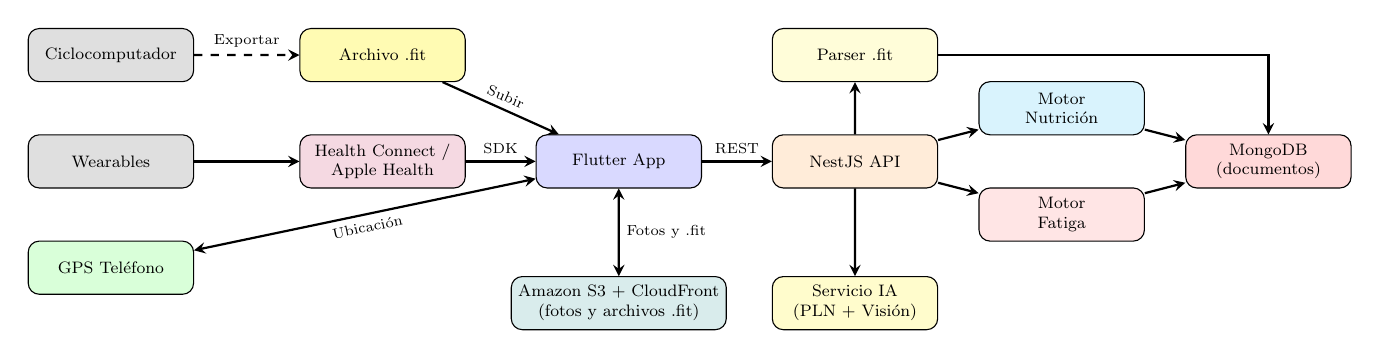
\begin{tikzpicture}[
    box/.style={draw, rectangle, rounded corners, minimum width=2.8cm, minimum height=0.9cm, fill=#1, align=center, font=\footnotesize},
    arrow/.style={->, thick, >=stealth},
    darrow/.style={<->, thick, >=stealth},
    dashed_arrow/.style={->, dashed, thick, >=stealth},
    lbl/.style={font=\scriptsize},
    scale=0.75, transform shape
]
    % Dispositivos del usuario
    \node (ciclo) [box=gray!25] at (-0.6,1.8) {Ciclocomputador};
    \node (wear) [box=gray!25] at (-0.6,0) {Wearables};
    \node (gps) [box=green!15] at (-0.6,-1.8) {GPS Teléfono};

    % Concentradores y archivo exportado
    \node (fit) [box=yellow!30] at (4,1.8) {Archivo .fit};
    \node (hc) [box=purple!15] at (4,0) {Health Connect /\\Apple Health};

    % Aplicación y almacenamiento de archivos
    \node (app) [box=blue!15] at (8,0) {Flutter App};
    \node (s3) [box=teal!15] at (8,-2.4) {Amazon S3 + CloudFront\\(fotos y archivos .fit)};

    % Backend
    \node (api) [box=orange!15] at (12,0) {NestJS API};
    \node (parser) [box=yellow!15] at (12,1.8) {Parser .fit};
    \node (ai) [box=yellow!20] at (12,-2.4) {Servicio IA\\(PLN + Visión)};
    \node (nutri) [box=cyan!15] at (15.5,0.9) {Motor\\Nutrición};
    \node (fatiga) [box=red!10] at (15.5,-0.9) {Motor\\Fatiga};

    % Base de datos
    \node (db) [box=red!15] at (19,0) {MongoDB\\(documentos)};

    % Flechas
    \draw[dashed_arrow] (ciclo) -- node[above, lbl] {Exportar} (fit);
    \draw[arrow] (wear) -- (hc);
    \draw[arrow] (fit) -- node[above, lbl, sloped] {Subir} (app);
    \draw[arrow] (hc) -- node[above, lbl] {SDK} (app);
    \draw[darrow] (gps) -- node[below, lbl, sloped] {Ubicación} (app);
    \draw[darrow] (app) -- node[right, lbl] {Fotos y .fit} (s3);
    \draw[arrow] (app) -- node[above, lbl] {REST} (api);
    \draw[arrow] (api) -- (parser);
    \draw[arrow] (api) -- (ai);
    \draw[arrow] (api) -- (nutri);
    \draw[arrow] (api) -- (fatiga);
    \draw[arrow] (nutri) -- (db);
    \draw[arrow] (fatiga) -- (db);
    \draw[arrow] (parser) -| (db);

\end{tikzpicture}
\captionof{figure}{Arquitectura de la Alternativa 3: Solución por Capas.}
\end{center}
\vspace{0.5cm}
\newpage
\textbf{Estimación de Costos}

La siguiente tabla resume los costos de esta alternativa. El costo de desarrollo viene del análisis por ciclo de vida (Tabla \ref{tab:ciclovida_alt3}), y los demás valores son los mismos que se usan en su flujo de caja dentro de la factibilidad económica.

\begin{table}[h!]
    \centering
    \renewcommand{\arraystretch}{1.4}
    \begin{tabular}{|m{4cm}|m{5.5cm}|r|}
        \hline
        \rowcolor[HTML]{EFEFEF}
        \textbf{Ítem} & \textbf{Detalle} & \textbf{Costo (CLP)} \\ \hline
        \multicolumn{3}{|l|}{\cellcolor[HTML]{E3F2FD}\textbf{Inversión inicial (Año 0)}} \\ \hline
        Desarrollo de software & 508 horas de trabajo según el ciclo de vida & \$16.109.800 \\ \hline
        Publicación en tiendas & Google Play y Apple Developer & \$120.602 \\ \hline
        \rowcolor[HTML]{E8F5E9}
        \textbf{Total inversión inicial} & & \textbf{\$16.230.402} \\ \hline
        \multicolumn{3}{|l|}{\cellcolor[HTML]{FFF3E0}\textbf{Costos operativos anuales (Años 1 a 4)}} \\ \hline
        Infraestructura Cloud & AWS (Fargate, Lambda, ALB, IP públicas, CloudWatch y S3 para archivos \texttt{.fit}) y MongoDB Atlas M10 (Tabla \ref{tab:costo_infra}) & \$2.124.158 \\ \hline
        Imágenes & S3 y CloudFront para las fotos de perfil y de las publicaciones (Tabla \ref{tab:costo_imagenes}) & \$70.027 \\ \hline
        APIs de IA & Gemini (uso anual) & \$641.916 \\ \hline
        Mantenimiento & 10\% del costo de desarrollo & \$1.610.980 \\ \hline
        Suscripción Apple & Renovación anual del Apple Developer Program & \$96.287 \\ \hline
        \rowcolor[HTML]{FFF3E0}
        \textbf{Total operativo anual} & & \textbf{\$4.543.368} \\ \hline
    \end{tabular}
    \caption{Estimación de costos de la Alternativa 3: Solución por Capas.}
    \label{tab:costos_alt3}
\end{table}

\textbf{Complejidad adicional:} Los registros de cardio llegan desde fuentes con niveles de detalle muy distintos (desde el GPS del teléfono hasta archivos \texttt{.fit} con miles de puntos). Para poder usarlos en conjunto hay que diseñar una base de datos flexible y un proceso que los deje en un formato común que el motor de fatiga pueda consultar.
\newpage
\subsubsection{Cuadro Comparativo de Alternativas}
La siguiente tabla resume las diferencias funcionales, técnicas y económicas entre las tres alternativas, como base para la elección que se hace en el estudio de factibilidad.

\begin{table}[h!]
    \centering
    \renewcommand{\arraystretch}{1.4}
    \begin{tabular}{|m{3.8cm}|m{3.5cm}|m{3.5cm}|m{3.8cm}|}
        \hline
        \rowcolor[HTML]{EFEFEF}
        \textbf{Dimensión} & \textbf{Alt. 1: Minimalista} & \textbf{Alt. 2: Brokers SO} & \textbf{Alt. 3: Por Capas} \\ \hline
        \textbf{Registro Nutricional} & Formulario manual & PLN + Visión IA & PLN + Visión IA + Escalado comunitario \\ \hline
        \textbf{Registro de Fuerza} & Formulario manual & Formulario + PLN & Formulario + PLN \\ \hline
        \textbf{Registro de Cardio} & GPS teléfono + RPE & GPS + Health Connect / Apple Health & GPS + Brokers + Archivo .fit \\ \hline
        \textbf{Frecuencia Cardíaca} & No disponible & Sí (vía broker) & Sí (broker + .fit segundo a segundo) \\ \hline
        \textbf{Potencia (ciclismo)} & No disponible & No disponible & Sí (vía archivo .fit) \\ \hline
        \textbf{Precisión del motor de fatiga} & Baja (volumen + RPE) & Media-Alta (zonas FC + calorías) & Alta (potencia + FC + TSS) \\ \hline
        \textbf{Módulo Social} & Básico (compartir) & Compartir con ajuste de recetas & Red social con contenido reutilizable en todos los módulos \\ \hline
        \textbf{Fotos que se guardan} & Solo perfil & Perfil y recetas & Perfil y publicaciones (hasta 4 por publicación) \\ \hline
        \textbf{Perfil y plan sugerido} & No & No & Sí \\ \hline
        \textbf{Uso de IA} & No & Sí (PLN + Visión) & Sí (PLN + Visión) \\ \hline
        \textbf{Tiempo de desarrollo} & 3-4 meses & 6-7 meses & 9-10 meses \\ \hline
        \textbf{Inversión inicial} & \$8.666.229 CLP & \$12.242.990 CLP & \$16.230.402 CLP \\ \hline
        \textbf{Costo operativo anual} & \$2.841.584 CLP & \$3.899.532 CLP & \$4.543.368 CLP \\ \hline
        \textbf{Complejidad técnica} & Baja & Media & Alta \\ \hline
        \textbf{Barrera de entrada usuario} & Ninguna (solo teléfono) & Baja (smartwatch opcional) & Ninguna (escala con hardware) \\ \hline
    \end{tabular}
    \caption{Cuadro comparativo de las alternativas de solución.}
    \label{tab:comparativa_alternativas}
\end{table}
\newpage
\subsection{Estudio de Factibilidad}
El estudio de factibilidad sirve para evaluar si la solución propuesta se puede llevar a cabo antes de invertir recursos en ella. Este análisis se divide en tres partes, que son la factibilidad técnica, la económica y la operativa. Con esta evaluación se busca identificar restricciones y riesgos a tiempo, y confirmar que se cuenta con la tecnología, el presupuesto y las condiciones necesarias para construir el sistema y desarrollar el Producto Mínimo Viable (MVP) con la alternativa elegida.

\subsubsection{Factibilidad Técnica}
La factibilidad técnica evalúa si se cuenta con la tecnología, la infraestructura y los conocimientos necesarios para desarrollar y mantener el sistema. Considerando que el proyecto integra varias fuentes de datos y usa inteligencia artificial, el análisis se hace desde los siguientes puntos de vista:
\newpage
\textbf{1. Disponibilidad del Stack Tecnológico:}\\
El sistema se basa en tecnologías maduras, de código abierto (open-source) y muy usadas en la industria. Esto reduce la dependencia de proveedores cerrados y facilita que el sistema pueda crecer más adelante.
\begin{itemize}
    \item Frontend: Flutter (mantenido por Google) tiene mucha documentación y una gran cantidad de paquetes de la comunidad (pub.dev) que facilitan el acceso al GPS, la cámara y el almacenamiento del teléfono, con un solo código para iOS y Android.
    \item Backend: NestJS, construido sobre Node.js y TypeScript, tiene una estructura por módulos que permite crear APIs REST y manejar servicios más complejos, como la lectura de archivos y los cálculos. Además, TypeScript es un lenguaje muy conocido, por lo que es fácil encontrar documentación y desarrolladores.
    \item Base de Datos: MongoDB es una de las bases de datos NoSQL más usadas. Cuenta con un servicio administrado en la nube (MongoDB Atlas), un driver oficial para Node.js y librerías como Mongoose que se integran con NestJS. Además, permite guardar series de tiempo de forma nativa, lo que sirve para la telemetría de los dispositivos. Las primeras pruebas del prototipo se hicieron con Firestore, otra base de datos orientada a documentos, y el modelo funcionó bien, lo que respalda este enfoque.
\end{itemize}

\textbf{2. Integración con Hardware y Concentradores (Brokers):}\\
Leer automáticamente los datos de cardio de los wearables es técnicamente posible. Tanto Google (con Health Connect) como Apple (con HealthKit) ofrecen Kits de Desarrollo de Software (SDKs) bien documentados, con los que una aplicación puede pedir permisos de lectura al usuario y acceder a datos como la frecuencia cardíaca, los pasos y las calorías. Además, Flutter cuenta con librerías de la comunidad que permiten usar ambas plataformas con un mismo código en Dart, lo que reduce bastante el trabajo de integración.
\newpage
\textbf{3. Inteligencia Artificial (PLN y Visión Artificial):}\\
Desarrollar y entrenar modelos propios de lenguaje natural o de reconocimiento de alimentos desde cero requeriría equipos con GPUs y especialistas en ciencia de datos, lo que haría inviable el MVP tanto en lo técnico como en lo económico.
\\\\
Sin embargo, usar APIs comerciales en la nube (como OpenAI, Google Gemini API o plataformas de análisis de alimentos como LogMeal) hace que esta función sea completamente factible. Estas plataformas funcionan como un servicio (AI as a Service). La aplicación solo tiene que enviar solicitudes HTTPS, el procesamiento pesado lo hacen los servidores del proveedor y la respuesta llega ordenada en formato JSON.
\\\\
\textbf{4. Procesamiento de Archivos .FIT:}\\
Leer archivos \texttt{.fit} de ciclocomputadores es factible porque el consorcio ANT+ publica su protocolo de forma abierta. Hoy existen varios paquetes de código abierto en lenguajes como JavaScript, TypeScript o Python que leen estos archivos binarios y los convierten en listas de datos para obtener la información segundo a segundo (potencia, cadencia). Por lo tanto, no es necesario programar el lector desde cero.
\\\\
\textbf{5. Red Social y Plan Sugerido:}\\
La red social se construye con funciones conocidas, como seguir usuarios, un muro de publicaciones paginado y la copia de una publicación al módulo de quien la ve. Las fotos de las publicaciones tampoco son un problema técnico. El teléfono las comprime antes de subirlas y las envía directamente a Amazon S3, el mismo almacenamiento de los archivos \texttt{.fit}, usando un permiso temporal que entrega el backend. En MongoDB solo queda su dirección, y para mostrarlas se usa Amazon CloudFront, que guarda copias cerca de los usuarios. Los videos se dejan para después del MVP, porque pesan mucho más y hay que procesarlos antes de mostrarlos. El plan sugerido tampoco exige técnicas complejas, ya que parte de plantillas definidas para cada perfil (nivel y orientación) que se ajustan con reglas simples según la adherencia, el RPE y la fatiga registrada.
\newpage
\textbf{Conclusión de Factibilidad Técnica:}\\
Se concluye que el proyecto es \textbf{técnicamente factible}. No requiere crear hardware nuevo, hacer descubrimientos científicos ni inventar algoritmos o lenguajes desde cero. La solución se basa en combinar servicios en la nube, SDKs públicos y frameworks que ya están probados, documentados y disponibles para cualquier desarrollador.

\subsubsection{Factibilidad Económica}
La factibilidad económica evalúa si el proyecto puede generar ingresos que justifiquen la inversión. Para cada alternativa se construye un flujo de caja proyectado a 4 años, y con él se calculan tres indicadores financieros, que son el Valor Actual Neto (VAN), la Tasa Interna de Retorno (TIR) y el Periodo de Recuperación de la Inversión (Payback).
\\\\
El objetivo es calcular, para cada alternativa, el \textbf{ingreso anual neto mínimo} con el que se logra al mismo tiempo un VAN igual a cero, una TIR del 15\% y un Payback dentro del cuarto año de operación.
\\\\
\textbf{Modelo de Ingresos}

La plataforma funcionará con un modelo de suscripción freemium. Habrá una versión gratuita con el registro manual y el plan sugerido, y para acceder a todo lo demás, que incluye la integración con wearables, la asistencia por IA, el cruce de datos, las alertas, las metas de alimentación y la red social, se deberá pagar una suscripción mensual premium. Tomando como referencia precios del mercado chileno (Fitia Premium a \$6.990 CLP al mes, Strava a \$7.600 CLP al mes y Freeletics a \$8.000 CLP al mes), se fija un precio de \textbf{\$7.990 CLP al mes}, es decir, \textbf{\$95.880 CLP al año} por usuario.
\\\\
Sin embargo, el proyecto no recibe ese monto completo. El precio incluye un IVA de 19\% \citep{sii_iva_digital}, por lo que sin IVA queda en \$6.714 CLP al mes. Además, el cobro se hace a través de Google Play y App Store, que cobran una comisión de hasta 15\% para desarrolladores con ingresos menores a un millón de dólares al año \citep{apple_small_business, google_service_fees}. Se considera el 15\% sobre el precio sin IVA, por lo que quedan \$5.707 CLP al mes por suscriptor. Es decir, el \textbf{ingreso neto por suscriptor es de \$68.486 CLP al año}, y este es el valor que se usa para calcular cuántos suscriptores se necesitan.
\newpage
\textbf{Breve Estudio Exploratorio de Mercado}

Para un producto enfocado en entrenamiento concurrente y nutrición, el tamaño del mercado en Chile se puede estimar de la siguiente forma \citep{mindep_habitos}:

\begin{itemize}
    \item \textbf{TAM (Mercado total, deportistas en Chile):} Según la Encuesta Nacional de Hábitos de Actividad Física y Deporte (MINDEP), entre el 32\% y el 35\% de la población mayor de 18 años hace actividad física de forma regular, lo que equivale a unos 4,5 a 5 millones de personas.
    \item \textbf{SAM (Mercado disponible, gimnasio, running y ciclismo):} Entre 1,2 y 1,5 millones de personas practican musculación, running o ciclismo. Dentro de este grupo, se estima que entre 180.000 y 250.000 personas hacen entrenamiento concurrente y usan smartphones junto con monitores de frecuencia cardíaca o GPS.
    \item \textbf{SOM (Mercado objetivo inicial):} Si se logra llegar a entre el 1\% y el 2\% del SAM en una primera etapa, se tendrían entre 1.800 y 5.000 usuarios activos. Para evaluar un escenario desfavorable, se considera una base de solo 1.500 usuarios, lo que equivale a menos del 1\% del SAM.
\end{itemize}

\vspace{0.3cm}
\textbf{El fenómeno de Hyrox y el atleta híbrido}

Las carreras de fitness híbrido, que combinan fuerza funcional con resistencia cardiovascular, son el mejor ejemplo de esta tendencia \citep{clarin_hyrox}.

\begin{itemize}
    \item La participación en Hyrox ha crecido muy rápido. Pasó de unos 650 competidores en su inicio en 2017 a más de 650.000 en 2024, y se proyecta que supere los 1,2 millones de atletas inscritos en la temporada 2025/2026 a nivel mundial.
    \item Un análisis de más de 275.000 atletas de esta modalidad mostró que atrae tanto a deportistas recreativos como de élite. Destaca la alta participación de personas mayores de 30 años y el crecimiento de la participación femenina, que ya ronda el 38\%.
    \item La preparación para estos eventos ha hecho que el entrenamiento concurrente se vuelva común en gimnasios tradicionales, donde los usuarios tienen que combinar sus sesiones de pesas con trabajo aeróbico intenso.
\end{itemize}

\vspace{0.3cm}
Además, el ACSM (American College of Sports Medicine), en su encuesta mundial de tendencias para 2026, mantiene al entrenamiento funcional y al uso de tecnología de datos (wearables) dentro de su Top 10. Según estos reportes, los usuarios se están alejando del enfoque solo estético y le dan más importancia a la funcionalidad, la longevidad y el rendimiento general \citep{acsm_trends}.
\\\\
Por su parte, el informe Year in Sport de Strava mostró que sus usuarios están probando cada vez más disciplinas distintas. El entrenamiento de fuerza fue la actividad que más creció entre las mujeres en la plataforma (con un aumento del 25\% en las actividades registradas), y al mismo tiempo la participación en clubes de running aumentó un 59\% \citep{strava_yis}.
\\\\
Por lo tanto, se concluye que una base inicial (SOM) de unos 1.500 posibles usuarios en Chile que hacen entrenamiento concurrente es razonable, y las fuentes indican que este número va en aumento.

\newpage
\textbf{Estimación de Costos por Ciclo de Vida del Desarrollo de Software}

Para respaldar los costos de desarrollo de cada alternativa, a continuación se presenta una estimación detallada basada en el ciclo de vida del software. El esfuerzo total se divide en cinco etapas. Las horas de trabajo (HH) se valorizaron con tarifas distintas según el cargo, obtenidas de una revisión del mercado laboral chileno en 2026 (portales como Computrabajo, Indeed e ITWorkers, entre otros). Estas tarifas van desde \textbf{\$12.320 CLP por hora} para asesores en la etapa de pruebas hasta \textbf{\$73.917 CLP por hora} para un Jefe de Proyecto Senior.

\begin{enumerate}
    \item \textbf{Análisis:} Levantamiento y especificación de los requerimientos funcionales y no funcionales, y definición del alcance y las restricciones del sistema.
    \item \textbf{Diseño Lógico:} Diseño de la arquitectura, modelo conceptual de la base de datos, definición de interfaces y API, y diseño de la experiencia de usuario (wireframes).
    \item \textbf{Diseño Físico:} Programación de todos los componentes del sistema, incluyendo frontend, backend, base de datos, integraciones y servicios de apoyo.
    \item \textbf{Pruebas QA:} Pruebas unitarias, de integración, funcionales y de rendimiento para asegurar la calidad del producto.
    \item \textbf{Implementación:} Configuración de la infraestructura, despliegue en la nube, publicación en las tiendas de aplicaciones y puesta en marcha del sistema.
\end{enumerate}
\newpage
\textbf{Ciclo de Vida de la Alternativa 1: Solución Minimalista}

\begin{table}[h!]
    \centering
    \renewcommand{\arraystretch}{1.15}
    \footnotesize
    \begin{tabular}{|l|c|r|r|r|}
        \hline
        \rowcolor[HTML]{EFEFEF}
        \textbf{Cargo} & \textbf{Cant.} & \textbf{Horas} & \textbf{VH (CLP)} & \textbf{Total (CLP)} \\ \hline
        \multicolumn{5}{|l|}{\cellcolor[HTML]{E3F2FD}\textbf{Etapa 1: Análisis}} \\ \hline
        JP Senior & 1 & 8 & \$73.917 & \$591.336 \\ \hline
        JP Junior & 1 & 6 & \$32.852 & \$197.112 \\ \hline
        Nutricionista/Coach Dep. (Asesor) & 1 & 6 & \$20.533 & \$123.195 \\ \hline
        \rowcolor[HTML]{F3F3F3}
        \multicolumn{4}{|r|}{\textbf{Subtotal Análisis}} & \textbf{\$911.643} \\ \hline
        \multicolumn{5}{|l|}{\cellcolor[HTML]{E3F2FD}\textbf{Etapa 2: Diseño Lógico}} \\ \hline
        JP Senior & 1 & 8 & \$73.917 & \$591.336 \\ \hline
        JP Junior & 1 & 14 & \$32.852 & \$459.928 \\ \hline
        Arquitecto Web & 1 & 24 & \$32.852 & \$788.448 \\ \hline
        Desarrollador UX/UI & 1 & 6 & \$28.746 & \$172.473 \\ \hline
        Nutricionista/Coach Dep. (Asesor) & 1 & 10 & \$12.320 & \$123.195 \\ \hline
        \rowcolor[HTML]{F3F3F3}
        \multicolumn{4}{|r|}{\textbf{Subtotal Diseño Lógico}} & \textbf{\$2.135.380} \\ \hline
        \multicolumn{5}{|l|}{\cellcolor[HTML]{E3F2FD}\textbf{Etapa 3: Diseño Físico}} \\ \hline
        JP Senior & 1 & 10 & \$73.917 & \$739.170 \\ \hline
        JP Junior & 1 & 10 & \$32.852 & \$328.520 \\ \hline
        Desarrollador UX/UI & 1 & 50 & \$28.746 & \$1.437.275 \\ \hline
        Desarrollador Backend & 1 & 50 & \$28.746 & \$1.437.275 \\ \hline
        Nutricionista/Coach Dep. (Asesor) & 1 & 6 & \$12.320 & \$73.917 \\ \hline
        \rowcolor[HTML]{F3F3F3}
        \multicolumn{4}{|r|}{\textbf{Subtotal Diseño Físico}} & \textbf{\$4.016.157} \\ \hline
        \multicolumn{5}{|l|}{\cellcolor[HTML]{E3F2FD}\textbf{Etapa 4: Pruebas QA}} \\ \hline
        JP Junior & 1 & 10 & \$32.852 & \$328.520 \\ \hline
        Ingeniero QA & 1 & 15 & \$24.639 & \$369.585 \\ \hline
        Nutricionista/Coach Dep. (Asesor) & 1 & 5 & \$12.320 & \$61.598 \\ \hline
        \rowcolor[HTML]{F3F3F3}
        \multicolumn{4}{|r|}{\textbf{Subtotal Pruebas QA}} & \textbf{\$759.703} \\ \hline
        \multicolumn{5}{|l|}{\cellcolor[HTML]{E3F2FD}\textbf{Etapa 5: Implementación}} \\ \hline
        JP Junior & 1 & 10 & \$32.852 & \$328.520 \\ \hline
        DevOps & 1 & 12 & \$32.852 & \$394.224 \\ \hline
        \rowcolor[HTML]{F3F3F3}
        \multicolumn{4}{|r|}{\textbf{Subtotal Implementación}} & \textbf{\$722.744} \\ \hline
        \rowcolor[HTML]{E8F5E9}
        \multicolumn{4}{|r|}{\textbf{TOTAL DESARROLLO PERSONAL}} & \textbf{\$8.545.627} \\ \hline
    \end{tabular}
    \caption{Desglose detallado de costos de personal por etapa: Alternativa 1.}
    \label{tab:ciclovida_alt1}
\end{table}
\newpage
\textbf{Ciclo de Vida de la Alternativa 2: Solución Integrada con Brokers}

\begin{table}[h!]
    \centering
    \renewcommand{\arraystretch}{1.15}
    \footnotesize
    \begin{tabular}{|l|c|r|r|r|}
        \hline
        \rowcolor[HTML]{EFEFEF}
        \textbf{Cargo} & \textbf{Cant.} & \textbf{Horas} & \textbf{VH (CLP)} & \textbf{Total (CLP)} \\ \hline
        \multicolumn{5}{|l|}{\cellcolor[HTML]{E3F2FD}\textbf{Etapa 1: Análisis}} \\ \hline
        JP Senior & 1 & 8 & \$73.917 & \$591.336 \\ \hline
        JP Junior & 1 & 6 & \$32.852 & \$197.112 \\ \hline
        Nutricionista/Coach Dep. (Asesor) & 1 & 6 & \$20.533 & \$123.195 \\ \hline
        Científico de Datos / IA & 1 & 6 & \$28.746 & \$172.473 \\ \hline
        \rowcolor[HTML]{F3F3F3}
        \multicolumn{4}{|r|}{\textbf{Subtotal Análisis}} & \textbf{\$1.084.116} \\ \hline
        \multicolumn{5}{|l|}{\cellcolor[HTML]{E3F2FD}\textbf{Etapa 2: Diseño Lógico}} \\ \hline
        JP Senior & 1 & 8 & \$73.917 & \$591.336 \\ \hline
        JP Junior & 1 & 14 & \$32.852 & \$459.928 \\ \hline
        Arquitecto Web & 1 & 28 & \$32.852 & \$919.856 \\ \hline
        Desarrollador UX/UI & 1 & 6 & \$28.746 & \$172.473 \\ \hline
        Nutricionista/Coach Dep. (Asesor) & 1 & 14 & \$12.320 & \$172.473 \\ \hline
        Científico de Datos / IA & 1 & 8 & \$28.746 & \$229.964 \\ \hline
        \rowcolor[HTML]{F3F3F3}
        \multicolumn{4}{|r|}{\textbf{Subtotal Diseño Lógico}} & \textbf{\$2.546.030} \\ \hline
        \multicolumn{5}{|l|}{\cellcolor[HTML]{E3F2FD}\textbf{Etapa 3: Diseño Físico}} \\ \hline
        JP Senior & 1 & 10 & \$73.917 & \$739.170 \\ \hline
        JP Junior & 1 & 14 & \$32.852 & \$459.928 \\ \hline
        Desarrollador UX/UI & 1 & 60 & \$28.746 & \$1.724.730 \\ \hline
        Desarrollador Backend & 1 & 60 & \$28.746 & \$1.724.730 \\ \hline
        Nutricionista/Coach Dep. (Asesor) & 1 & 6 & \$12.320 & \$73.917 \\ \hline
        Científico de Datos / IA & 1 & 30 & \$28.746 & \$862.365 \\ \hline
        Desarrollador Mobile & 1 & 30 & \$28.746 & \$862.365 \\ \hline
        Ingeniero DB & 1 & 15 & \$28.746 & \$431.183 \\ \hline
        \rowcolor[HTML]{F3F3F3}
        \multicolumn{4}{|r|}{\textbf{Subtotal Diseño Físico}} & \textbf{\$6.878.388} \\ \hline
        \multicolumn{5}{|l|}{\cellcolor[HTML]{E3F2FD}\textbf{Etapa 4: Pruebas QA}} \\ \hline
        JP Junior & 1 & 10 & \$32.852 & \$328.520 \\ \hline
        Ingeniero QA & 1 & 15 & \$24.639 & \$369.585 \\ \hline
        Nutricionista/Coach Dep. (Asesor) & 1 & 5 & \$12.320 & \$61.598 \\ \hline
        \rowcolor[HTML]{F3F3F3}
        \multicolumn{4}{|r|}{\textbf{Subtotal Pruebas QA}} & \textbf{\$759.703} \\ \hline
        \multicolumn{5}{|l|}{\cellcolor[HTML]{E3F2FD}\textbf{Etapa 5: Implementación}} \\ \hline
        JP Junior & 1 & 12 & \$32.852 & \$394.224 \\ \hline
        DevOps & 1 & 14 & \$32.852 & \$459.928 \\ \hline
        \rowcolor[HTML]{F3F3F3}
        \multicolumn{4}{|r|}{\textbf{Subtotal Implementación}} & \textbf{\$854.152} \\ \hline
        \rowcolor[HTML]{E8F5E9}
        \multicolumn{4}{|r|}{\textbf{TOTAL DESARROLLO PERSONAL}} & \textbf{\$12.122.388} \\ \hline
    \end{tabular}
    \caption{Desglose detallado de costos de personal por etapa: Alternativa 2.}
    \label{tab:ciclovida_alt2}
\end{table}

\newpage
\textbf{Ciclo de Vida de la Alternativa 3: Solución por Capas}

\begin{table}[h!]
    \centering
    \renewcommand{\arraystretch}{1.15}
    \footnotesize
    \begin{tabular}{|l|c|r|r|r|}
        \hline
        \rowcolor[HTML]{EFEFEF}
        \textbf{Cargo} & \textbf{Cant.} & \textbf{Horas} & \textbf{VH (CLP)} & \textbf{Total (CLP)} \\ \hline
        \multicolumn{5}{|l|}{\cellcolor[HTML]{E3F2FD}\textbf{Etapa 1: Análisis}} \\ \hline
        JP Senior & 1 & 14 & \$73.917 & \$1.034.838 \\ \hline
        JP Junior & 1 & 10 & \$32.852 & \$328.520 \\ \hline
        Nutricionista/Coach Dep. (Asesor) & 1 & 6 & \$20.533 & \$123.195 \\ \hline
        Científico de Datos / IA & 1 & 6 & \$28.746 & \$172.473 \\ \hline
        Esp. Telemetría Wearables & 1 & 6 & \$28.746 & \$172.473 \\ \hline
        \rowcolor[HTML]{F3F3F3}
        \multicolumn{4}{|r|}{\textbf{Subtotal Análisis}} & \textbf{\$1.831.499} \\ \hline
        \multicolumn{5}{|l|}{\cellcolor[HTML]{E3F2FD}\textbf{Etapa 2: Diseño Lógico}} \\ \hline
        JP Senior & 1 & 12 & \$73.917 & \$887.004 \\ \hline
        JP Junior & 1 & 20 & \$32.852 & \$657.040 \\ \hline
        Arquitecto Web & 1 & 32 & \$32.852 & \$1.051.264 \\ \hline
        Desarrollador UX/UI & 1 & 6 & \$28.746 & \$172.473 \\ \hline
        Nutricionista/Coach Dep. (Asesor) & 1 & 20 & \$12.320 & \$246.390 \\ \hline
        Científico de Datos / IA & 1 & 10 & \$28.746 & \$287.455 \\ \hline
        \rowcolor[HTML]{F3F3F3}
        \multicolumn{4}{|r|}{\textbf{Subtotal Diseño Lógico}} & \textbf{\$3.301.626} \\ \hline
        \multicolumn{5}{|l|}{\cellcolor[HTML]{E3F2FD}\textbf{Etapa 3: Diseño Físico}} \\ \hline
        JP Senior & 1 & 10 & \$73.917 & \$739.170 \\ \hline
        JP Junior & 1 & 20 & \$32.852 & \$657.040 \\ \hline
        Desarrollador UX/UI & 1 & 70 & \$28.746 & \$2.012.185 \\ \hline
        Desarrollador Backend & 1 & 70 & \$28.746 & \$2.012.185 \\ \hline
        Nutricionista/Coach Dep. (Asesor) & 1 & 6 & \$12.320 & \$73.917 \\ \hline
        Científico de Datos / IA & 1 & 40 & \$28.746 & \$1.149.820 \\ \hline
        Desarrollador Mobile & 1 & 35 & \$28.746 & \$1.006.093 \\ \hline
        Esp. Telemetría Wearables & 1 & 35 & \$28.746 & \$1.006.093 \\ \hline
        Ingeniero DB & 1 & 20 & \$28.746 & \$574.910 \\ \hline
        \rowcolor[HTML]{F3F3F3}
        \multicolumn{4}{|r|}{\textbf{Subtotal Diseño Físico}} & \textbf{\$9.231.412} \\ \hline
        \multicolumn{5}{|l|}{\cellcolor[HTML]{E3F2FD}\textbf{Etapa 4: Pruebas QA}} \\ \hline
        JP Junior & 1 & 10 & \$32.852 & \$328.520 \\ \hline
        Ingeniero QA & 1 & 15 & \$24.639 & \$369.585 \\ \hline
        Nutricionista/Coach Dep. (Asesor) & 1 & 5 & \$12.320 & \$61.598 \\ \hline
        \rowcolor[HTML]{F3F3F3}
        \multicolumn{4}{|r|}{\textbf{Subtotal Pruebas QA}} & \textbf{\$759.703} \\ \hline
        \multicolumn{5}{|l|}{\cellcolor[HTML]{E3F2FD}\textbf{Etapa 5: Implementación}} \\ \hline
        JP Junior & 1 & 14 & \$32.852 & \$459.928 \\ \hline
        DevOps & 1 & 16 & \$32.852 & \$525.632 \\ \hline
        \rowcolor[HTML]{F3F3F3}
        \multicolumn{4}{|r|}{\textbf{Subtotal Implementación}} & \textbf{\$985.560} \\ \hline
        \rowcolor[HTML]{E8F5E9}
        \multicolumn{4}{|r|}{\textbf{TOTAL DESARROLLO PERSONAL}} & \textbf{\$16.109.800} \\ \hline
    \end{tabular}
    \caption{Desglose detallado de costos de personal por etapa: Alternativa 3.}
    \label{tab:ciclovida_alt3}
\end{table}

\newpage
\textbf{Resumen Comparativo de Costos por Ciclo de Vida}

La siguiente tabla resume cómo se reparte el costo de personal en cada etapa del ciclo de vida para las tres alternativas.
\begin{table}[h!]
    \centering
    \renewcommand{\arraystretch}{1.4}
    \footnotesize
    \begin{tabular}{|m{2.8cm}|r|r|r|}
        \hline
        \rowcolor[HTML]{EFEFEF}
        \textbf{Etapa (miles CLP)} & \textbf{Alternativa 1} & \textbf{Alternativa 2} & \textbf{Alternativa 3} \\ \hline
        Análisis & \$912 & \$1.084& \$1.831 \\ \hline
        Diseño Lógico & \$2.135 & \$2.546 & \$3.302 \\ \hline
        Diseño Físico & \$4.016 & \$6.878 & \$9.231 \\ \hline
        Pruebas QA & \$760 & \$760 & \$760 \\ \hline
        Implementación & \$723 & \$854 & \$986 \\ \hline
        \rowcolor[HTML]{E8F5E9}
        \textbf{TOTAL} & \textbf{\$8.546} & \textbf{\$12.122} & \textbf{\$16.110} \\ \hline
    \end{tabular}
    \caption{Resumen comparativo de costos por ciclo de vida (valores en miles de CLP).}
    \label{tab:resumen_ciclovida}
\end{table}

\newpage
\textbf{Estructura de Costos: Inversión Inicial vs. Costos Operativos}

Para armar el flujo de caja, los costos se separan en dos grupos. El primero es la \textbf{inversión inicial} (Año 0), que incluye el desarrollo y la publicación inicial en las tiendas de aplicaciones. El segundo son los \textbf{costos operativos anuales} (Años 1 a 4), que incluyen la infraestructura en la nube (AWS Fargate, ALB y S3, junto con la base de datos administrada), el almacenamiento y la entrega de imágenes, el uso de APIs de IA (Gemini), la renovación del Apple Developer Program y un 10\% del costo de desarrollo para mantenimiento. Los videos no se consideran, porque quedan fuera del MVP.

\begin{table}[h!]
    \centering
    \renewcommand{\arraystretch}{1.4}
    \begin{tabular}{|m{4.5cm}|r|r|r|}
        \hline
        \rowcolor[HTML]{EFEFEF}
        \textbf{Concepto} & \textbf{Alt. 1} & \textbf{Alt. 2} & \textbf{Alt. 3} \\ \hline
        \multicolumn{4}{|l|}{\cellcolor[HTML]{E3F2FD}\textbf{Inversión Inicial (Año 0)}} \\ \hline
        Desarrollo de software & \$8.545.627 & \$12.122.388 & \$16.109.800 \\ \hline
        Publicación inicial tiendas & \$120.602 & \$120.602 & \$120.602 \\ \hline
        \rowcolor[HTML]{E8F5E9}
        \textbf{Total Inversión ($I_0$)} & \textbf{\$8.666.229} & \textbf{\$12.242.990} & \textbf{\$16.230.402} \\ \hline
        \multicolumn{4}{|l|}{\cellcolor[HTML]{FFF3E0}\textbf{Costos Operativos Anuales (Años 1--4)}} \\ \hline
        Infraestructura Cloud & \$1.879.063 & \$2.112.487 & \$2.124.158 \\ \hline
        Imágenes (S3 y CloudFront) & \$11.671 & \$11.671 & \$70.027 \\ \hline
        APIs de IA (Gemini) & --- & \$466.848 & \$641.916 \\ \hline
        Mantenimiento (10\% dev) & \$854.563 & \$1.212.239 & \$1.610.980 \\ \hline
        Suscripción Apple (anual) & \$96.287 & \$96.287 & \$96.287 \\ \hline
        \rowcolor[HTML]{FFF3E0}
        \textbf{Total Operativo ($C_{op}$)} & \textbf{\$2.841.584} & \textbf{\$3.899.532} & \textbf{\$4.543.368} \\ \hline
    \end{tabular}
    \caption{Desglose de costos por categoría para cada alternativa (en CLP).}
    \label{tab:desglose_costos}
\end{table}
\newpage
\textbf{Costo de la Infraestructura en la Nube}

La Tabla \ref{tab:costo_infra} detalla el costo de la infraestructura de cada alternativa. Se calculó con los precios publicados por AWS para la región de São Paulo \citep{aws_fargate_pricing}, y al tipo de cambio de \$972,60 CLP por dólar. Las tres alternativas usan un clúster MongoDB Atlas M10, porque es el nivel más bajo que permite una conexión privada con la red de AWS, algo necesario al trabajar con datos sensibles. Su precio en São Paulo es una estimación, ya que MongoDB publica USD 57 al mes para Virginia \citep{atlas_pricing}. El dimensionamiento de la alternativa elegida se explica en el capítulo de diseño.

\begin{table}[h!]
    \centering
    \renewcommand{\arraystretch}{1.25}
    \footnotesize
    \begin{tabular}{|>{\raggedright\arraybackslash}p{7.2cm}|r|r|r|}
        \hline
        \rowcolor[HTML]{EFEFEF}
        \textbf{Componente (USD al mes)} & \textbf{Alt. 1} & \textbf{Alt. 2} & \textbf{Alt. 3} \\ \hline
        API en Fargate (Alt. 1: 0,25 vCPU y 0,5 GB. Alt. 2 y 3: 0,5 vCPU y 1 GB) & 16 & 31 & 31 \\ \hline
        Parser \texttt{.fit} en Lambda, dentro del nivel gratuito & --- & --- & 0 \\ \hline
        MongoDB Atlas M10, con almacenamiento y respaldos & 100 & 100 & 100 \\ \hline
        Balanceador de carga (ALB) & 27 & 29 & 29 \\ \hline
        Direcciones IP públicas & 11 & 11 & 11 \\ \hline
        CloudWatch & 3 & 5 & 5 \\ \hline
        S3, sin contar las fotos & --- & 1 & 2 \\ \hline
        Secrets Manager, ECR y dominio & 4 & 4 & 4 \\ \hline
        \rowcolor[HTML]{FFF3E0}
        \textbf{Total infraestructura (USD al mes)} & \textbf{161} & \textbf{181} & \textbf{182} \\ \hline
        \rowcolor[HTML]{FFF3E0}
        \textbf{Total infraestructura (CLP al año)} & \textbf{\$1.879.063} & \textbf{\$2.112.487} & \textbf{\$2.124.158} \\ \hline
    \end{tabular}
    \caption{Costo de la infraestructura en la nube por alternativa.}
    \label{tab:costo_infra}
\end{table}
\newpage
\textbf{Costo de Almacenamiento y Entrega de Imágenes}

El costo de las fotos se estimó por separado, porque depende de cuántas imágenes guarda cada alternativa. Se usaron los precios de Amazon S3 en la región de São Paulo, que son USD 0,0405 por GB al mes y USD 0,007 por cada 1.000 subidas \citep{aws_s3_pricing}, y el nivel gratuito permanente de CloudFront, que incluye 1 TB de transferencia y 10 millones de solicitudes al mes \citep{aws_cloudfront_pricing}. Los supuestos son los siguientes:

\begin{itemize}
    \item Una base de 1.500 usuarios, igual al mercado objetivo inicial (SOM).
    \item Cada foto pesa unos 300 KB después de comprimirla, más una miniatura de 40 KB.
    \item En la Alternativa 2, el 10\% de los usuarios comparte 2 recetas con foto al mes.
    \item En la Alternativa 3, el 40\% de los usuarios publica 6 veces al mes con 2 fotos en promedio.
    \item Cada usuario ve unas 30 fotos al día en el muro, la mayoría como miniatura.
\end{itemize}

Como las fotos se acumulan, el costo crece año a año. Para tener un margen, se toma el costo del cuarto año, que es el más alto, se redondea hacia arriba y se aplica igual en todos los años.

\begin{table}[h!]
    \centering
    \renewcommand{\arraystretch}{1.4}
    \footnotesize
    \begin{tabular}{|>{\raggedright\arraybackslash}m{4.8cm}|>{\raggedright\arraybackslash}m{3cm}|>{\raggedright\arraybackslash}m{3cm}|>{\raggedright\arraybackslash}m{3.4cm}|}
        \hline
        \rowcolor[HTML]{EFEFEF}
        \textbf{Concepto} & \textbf{Alt. 1} & \textbf{Alt. 2} & \textbf{Alt. 3} \\ \hline
        Fotos que se guardan & Solo perfil & Perfil y recetas (1 foto) & Perfil y publicaciones (hasta 4 fotos) \\ \hline
        Fotos nuevas al mes & Solo nuevos perfiles & Unas 300 & Unas 7.200 \\ \hline
        Espacio acumulado al cuarto año & 0,4 GB & 5 GB & 118 GB \\ \hline
        Almacenamiento en S3 (USD/mes) & 0,02 & 0,2 & 4,8 \\ \hline
        Subidas a S3 (USD/mes) & 0,01 & 0,01 & 0,1 \\ \hline
        Entrega por CloudFront (USD/mes) & 0 & 0 & 0 (unos 110 GB y 1,4 millones de solicitudes al mes, dentro del nivel gratuito) \\ \hline
        \rowcolor[HTML]{FFF3E0}
        \textbf{Costo considerado (USD/mes)} & \textbf{1} & \textbf{1} & \textbf{6} \\ \hline
        \rowcolor[HTML]{FFF3E0}
        \textbf{Costo anual (CLP, a \$972,60 por USD)} & \textbf{\$11.671} & \textbf{\$11.671} & \textbf{\$70.027} \\ \hline
    \end{tabular}
    \caption{Estimación del costo de almacenamiento y entrega de imágenes.}
    \label{tab:costo_imagenes}
\end{table}

El costo de las imágenes es bajo incluso en la Alternativa 3, porque las fotos se comprimen en el teléfono y CloudFront entrega gratis el volumen esperado. Si la aplicación creciera mucho más allá del mercado objetivo, la entrega de fotos superaría el nivel gratuito, pero en ese escenario también habría muchos más suscriptores para cubrirla.
\newpage

\textbf{Formulación del Análisis Financiero}

Las tres métricas utilizadas se definen a continuación:

\begin{itemize}
    \item \textbf{Valor Actual Neto (VAN):} Es el valor que tienen hoy todos los flujos de caja futuros, descontados a una tasa $r$, menos la inversión inicial. Un VAN $\geq 0$ indica que el proyecto genera valor.
    \begin{equation}
        VAN = -I_0 + \sum_{t=1}^{n} \frac{FC_t}{(1+r)^t}
    \end{equation}

    \item \textbf{Tasa Interna de Retorno (TIR):} Es la tasa de descuento $r^*$ con la que el VAN queda exactamente en cero. Si la TIR es mayor que la tasa mínima que exige el inversionista, el proyecto es rentable.
    \begin{equation}
        0 = -I_0 + \sum_{t=1}^{n} \frac{FC_t}{(1+r^*)^t}
    \end{equation}

    \item \textbf{Periodo de Recuperación (Payback):} Es el tiempo que se demora la suma de los flujos netos en igualar la inversión inicial.
    \begin{equation}
        Payback = t \text{ tal que } \sum_{k=1}^{t} FC_k \geq I_0
    \end{equation}
\end{itemize}

\textbf{Impuesto a la Renta y Amortización}

Las utilidades del proyecto pagan el Impuesto de Primera Categoría, que en el régimen general es de un 27\% \citep{sii_tasas}. El impuesto se calcula sobre la utilidad, por lo que antes se puede descontar la inversión. El software hecho a medida no se deprecia como un activo físico, sino que se trata como un gasto diferido, que se puede amortizar hasta en seis años \citep{sii_software}. Aquí se amortiza toda la inversión inicial en partes iguales durante los 4 años del horizonte ($A = I_0 \div 4$). La amortización no es una salida real de dinero, así que se resta para calcular el impuesto y se vuelve a sumar para obtener el flujo neto.
\\\\
Se usa la tasa del régimen general porque es el caso más conservador. Una empresa pequeña podría acogerse al régimen Pro Pyme, que tiene una tasa menor \citep{sii_tasas}, lo que reduciría los suscriptores requeridos. Esta opción y la forma de amortizar se deben confirmar con un contador antes de operar.

\textbf{Cálculo del Ingreso Mínimo Requerido}

Para obtener el ingreso anual neto ($R$) que cumple las condiciones definidas (VAN = 0, TIR = 15\% y Payback $\leq$ 4 años), se parte del flujo de caja neto constante ($FC$) que recupera la inversión:
\begin{equation}
    FC = \frac{I_0}{\displaystyle\sum_{t=1}^{4} \frac{1}{(1{,}15)^t}} = \frac{I_0}{2{,}8550}
\end{equation}
Con el impuesto, el flujo neto es la utilidad después de impuesto más la amortización, es decir, $FC = (R - C_{op} - A)(1 - 0{,}27) + A$. Despejando el ingreso requerido se obtiene:
\begin{equation}
    R = C_{op} + A + \frac{FC - A}{1 - 0{,}27}
\end{equation}

\newpage
\textbf{Flujo de Caja Proyectado de la Alternativa 1: Solución Minimalista}

$FC_1 = 8.666.229 \div 2{,}8550 = \$3.035.457$ CLP/año.\\
Amortización anual: $A_1 = 8.666.229 \div 4 = \$2.166.557$ CLP/año.\\
Ingreso anual neto requerido por suscripciones:\\ $R_1 = 2.841.584 + 2.166.557 + (3.035.457 - 2.166.557) \div 0{,}73 = \$6.198.415$ CLP/año.




\begin{table}[h!]
    \centering
    \renewcommand{\arraystretch}{1.3}
    \footnotesize
    \begin{tabular}{|m{3.2cm}|r|r|r|r|r|}
        \hline
        \rowcolor[HTML]{EFEFEF}
        \textbf{Concepto (CLP)} & \textbf{Año 0} & \textbf{Año 1} & \textbf{Año 2} & \textbf{Año 3} & \textbf{Año 4} \\ \hline
        
        \textbf{Ingresos } &&&&&\\ \hline
        Suscripciones (neto) & --- & 6.198.415 & 6.198.415 & 6.198.415 & 6.198.415 \\ \hline
        \rowcolor[HTML]{E8F5E9}
        \textbf{Total Ingresos} & --- & 6.198.415 & 6.198.415 & 6.198.415 & 6.198.415 \\ \hline
        & & & & & \\ \hline
        \textbf{Egresos} & & & & & \\ \hline
        Infraestructura & --- & -1.879.063 & -1.879.063 & -1.879.063 & -1.879.063 \\ \hline
        Imágenes & --- & -11.671 & -11.671 & -11.671 & -11.671 \\ \hline
        APIs de IA & --- & --- & --- & --- & --- \\ \hline
        Mantenimiento & --- & -854.563 & -854.563 & -854.563 & -854.563 \\ \hline
        Apple Developer & --- & -96.287 & -96.287 & -96.287 & -96.287 \\ \hline
        \rowcolor[HTML]{F3E5F5}
        \textbf{Total Egresos} & --- & -2.841.584 & -2.841.584 & -2.841.584 & -2.841.584 \\ \hline
        & & & & & \\ \hline
        Amortización & --- & -2.166.557 & -2.166.557 & -2.166.557 & -2.166.557 \\ \hline
        \textbf{Utilidad antes de impuesto} & --- & \textbf{1.190.274} & \textbf{1.190.274} & \textbf{1.190.274} & \textbf{1.190.274} \\ \hline
        Impuesto (27\%) & --- & -321.374 & -321.374 & -321.374 & -321.374 \\ \hline
        \textbf{Utilidad después de impuesto} & --- & \textbf{868.900} & \textbf{868.900} & \textbf{868.900} & \textbf{868.900} \\ \hline
        Suma de la amortización & --- & 2.166.557 & 2.166.557 & 2.166.557 & 2.166.557 \\ \hline
        & & & & & \\ \hline
        Valor Desarrollo & -8.545.627 & --- & --- & --- & --- \\ \hline
        Valor Publicación & -120.602 & --- & --- & --- & --- \\ \hline
        \rowcolor[HTML]{F3E5F5} 
        Inversión Inicial & -8.666.229 & --- & --- & --- & --- \\ \hline
        & & & & & \\ \hline
        \rowcolor[HTML]{E8F5E9}
        \textbf{Flujo Neto} & \textbf{-8.666.229} & \textbf{3.035.457} & \textbf{3.035.457} & \textbf{3.035.457} & \textbf{3.035.457} \\ \hline
        Flujo Acumulado & -8.666.229 & -5.630.772 & -2.595.315 & 440.142 & 3.475.599 \\ \hline
        \rowcolor[HTML]{F3E5F5}
        Factor $(1{,}15)^{-t}$ & 1,000 & 0,870 & 0,756 & 0,658 & 0,572 \\ \hline
        \rowcolor[HTML]{F3E5F5}
        Flujo Descontado & -8.666.229 & 2.639.528 & 2.295.242 & 1.995.862 & 1.735.532 \\ \hline
    \end{tabular}
    \caption{Flujo de caja a 4 años - Alternativa 1.}
    \label{tab:flujo_alt1}
\end{table}

\begin{center}
\begin{tabular}{lll}
    $VAN_{15\%}$ = \$0 CLP \quad & $TIR$ = \textbf{15,0\%} \quad & $Payback$ = \textbf{2,85 años}
\end{tabular}
\end{center}

Suscriptores pagos requeridos: $6.198.415 \div 68.486 = 90,51$, lo que se redondea hacia arriba a \textbf{91 usuarios premium/año} para alcanzar el equilibrio.
Esto representa un \textbf{6,07\%} de la base conservadora de 1.500 posibles usuarios (SOM).

\newpage
\textbf{Flujo de Caja Proyectado de la Alternativa 2: Solución Integrada con Brokers}

$FC_2 = 12.242.990 \div 2{,}8550 = \$4.288.263$ CLP/año.\\
Amortización anual: $A_2 = 12.242.990 \div 4 = \$3.060.748$ CLP/año.\\
Ingreso anual neto requerido por suscripciones:\\ $R_2 = 3.899.532 + 3.060.748 + (4.288.263 - 3.060.748) \div 0{,}73 = \$8.641.807$ CLP/año.

\begin{table}[h!]
    \centering
    \renewcommand{\arraystretch}{1.3}
    \footnotesize
    \begin{tabular}{|m{3.2cm}|r|r|r|r|r|}
        \hline
        \rowcolor[HTML]{EFEFEF}
        \textbf{Concepto (CLP)} & \textbf{Año 0} & \textbf{Año 1} & \textbf{Año 2} & \textbf{Año 3} & \textbf{Año 4} \\ \hline
        
        \textbf{Ingresos } &&&&&\\ \hline
        Suscripciones (neto) & --- & 8.641.807 & 8.641.807 & 8.641.807 & 8.641.807 \\ \hline
        \rowcolor[HTML]{E8F5E9}
        \textbf{Total Ingresos} & --- & 8.641.807 & 8.641.807 & 8.641.807 & 8.641.807 \\ \hline
        & & & & & \\ \hline
        \textbf{Egresos} & & & & & \\ \hline
        Infraestructura & --- & -2.112.487 & -2.112.487 & -2.112.487 & -2.112.487 \\ \hline
        Imágenes & --- & -11.671 & -11.671 & -11.671 & -11.671 \\ \hline
        APIs de IA & --- & -466.848 & -466.848 & -466.848 & -466.848 \\ \hline
        Mantenimiento & --- & -1.212.239 & -1.212.239 & -1.212.239 & -1.212.239 \\ \hline
        Apple Developer & --- & -96.287 & -96.287 & -96.287 & -96.287 \\ \hline
        \rowcolor[HTML]{F3E5F5}
        \textbf{Total Egresos} & --- & -3.899.532 & -3.899.532 & -3.899.532 & -3.899.532 \\ \hline
        & & & & & \\ \hline
        Amortización & --- & -3.060.748 & -3.060.748 & -3.060.748 & -3.060.748 \\ \hline
        \textbf{Utilidad antes de impuesto} & --- & \textbf{1.681.527} & \textbf{1.681.527} & \textbf{1.681.527} & \textbf{1.681.527} \\ \hline
        Impuesto (27\%) & --- & -454.012 & -454.012 & -454.012 & -454.012 \\ \hline
        \textbf{Utilidad después de impuesto} & --- & \textbf{1.227.515} & \textbf{1.227.515} & \textbf{1.227.515} & \textbf{1.227.515} \\ \hline
        Suma de la amortización & --- & 3.060.748 & 3.060.748 & 3.060.748 & 3.060.748 \\ \hline
        & & & & & \\ \hline
        Valor Desarrollo & -12.122.388 & --- & --- & --- & --- \\ \hline
        Valor Publicación & -120.602 & --- & --- & --- & --- \\ \hline
        \rowcolor[HTML]{F3E5F5} 
        Inversión Inicial & -12.242.990 & --- & --- & --- & --- \\ \hline
        & & & & & \\ \hline
        \rowcolor[HTML]{E8F5E9}
        \textbf{Flujo Neto} & \textbf{-12.242.990} & \textbf{4.288.263} & \textbf{4.288.263} & \textbf{4.288.263} & \textbf{4.288.263} \\ \hline
        Flujo Acumulado & -12.242.990 & -7.954.727 & -3.666.464 & 621.799 & 4.910.062 \\ \hline
        \rowcolor[HTML]{F3E5F5}
        Factor $(1{,}15)^{-t}$ & 1,000 & 0,870 & 0,756 & 0,658 & 0,572 \\ \hline
        \rowcolor[HTML]{F3E5F5}
        Flujo Descontado & -12.242.990 & 3.728.924 & 3.242.543 & 2.819.603 & 2.451.828 \\ \hline
    \end{tabular}
    \caption{Flujo de caja a 4 años - Alternativa 2.}
    \label{tab:flujo_alt2}
\end{table}

\begin{center}
\begin{tabular}{lll}
    $VAN_{15\%}$ = \$0 CLP \quad & $TIR$ = \textbf{15,0\%} \quad & $Payback$ = \textbf{2,85 años}
\end{tabular}
\end{center}

Suscriptores pagos requeridos: $8.641.807 \div 68.486 = 126,18$, lo que se redondea hacia arriba a \textbf{127 usuarios premium/año} para alcanzar el equilibrio.
Esto representa un \textbf{8,47\%} de la base conservadora de 1.500 posibles usuarios (SOM).

\newpage
\textbf{Flujo de Caja Proyectado de la Alternativa 3: Solución por Capas}

$FC_3 = 16.230.402 \div 2{,}8550 = \$5.684.904$ CLP/año.\\
Amortización anual: $A_3 = 16.230.402 \div 4 = \$4.057.601$ CLP/año.\\
Ingreso anual neto requerido por suscripciones:\\ $R_3 = 4.543.368 + 4.057.601 + (5.684.904 - 4.057.601) \div 0{,}73 = \$10.830.151$ CLP/año.

\begin{table}[h!]
    \centering
    \renewcommand{\arraystretch}{1.3}
    \footnotesize
    \begin{tabular}{|m{3.2cm}|r|r|r|r|r|}
        \hline
        \rowcolor[HTML]{EFEFEF}
        \textbf{Concepto (CLP)} & \textbf{Año 0} & \textbf{Año 1} & \textbf{Año 2} & \textbf{Año 3} & \textbf{Año 4} \\ \hline
        
        \textbf{Ingresos } &&&&&\\ \hline
        Suscripciones (neto) & --- & 10.830.151 & 10.830.151 & 10.830.151 & 10.830.151 \\ \hline
        \rowcolor[HTML]{E8F5E9}
        \textbf{Total Ingresos} & --- & 10.830.151 & 10.830.151 & 10.830.151 & 10.830.151 \\ \hline
        & & & & & \\ \hline
        \textbf{Egresos} & & & & & \\ \hline
        Infraestructura & --- & -2.124.158 & -2.124.158 & -2.124.158 & -2.124.158 \\ \hline
        Imágenes & --- & -70.027 & -70.027 & -70.027 & -70.027 \\ \hline
        APIs de IA & --- & -641.916 & -641.916 & -641.916 & -641.916 \\ \hline
        Mantenimiento & --- & -1.610.980 & -1.610.980 & -1.610.980 & -1.610.980 \\ \hline
        Apple Developer & --- & -96.287 & -96.287 & -96.287 & -96.287 \\ \hline
        \rowcolor[HTML]{F3E5F5}
        \textbf{Total Egresos} & --- & -4.543.368 & -4.543.368 & -4.543.368 & -4.543.368 \\ \hline
        & & & & & \\ \hline
        Amortización & --- & -4.057.601 & -4.057.601 & -4.057.601 & -4.057.601 \\ \hline
        \textbf{Utilidad antes de impuesto} & --- & \textbf{2.229.182} & \textbf{2.229.182} & \textbf{2.229.182} & \textbf{2.229.182} \\ \hline
        Impuesto (27\%) & --- & -601.879 & -601.879 & -601.879 & -601.879 \\ \hline
        \textbf{Utilidad después de impuesto} & --- & \textbf{1.627.303} & \textbf{1.627.303} & \textbf{1.627.303} & \textbf{1.627.303} \\ \hline
        Suma de la amortización & --- & 4.057.601 & 4.057.601 & 4.057.601 & 4.057.601 \\ \hline
        & & & & & \\ \hline
        Valor Desarrollo & -16.109.800 & --- & --- & --- & --- \\ \hline
        Valor Publicación & -120.602 & --- & --- & --- & --- \\ \hline
        \rowcolor[HTML]{F3E5F5} 
        Inversión Inicial & -16.230.402 & --- & --- & --- & --- \\ \hline
        & & & & & \\ \hline
        \rowcolor[HTML]{E8F5E9}
        \textbf{Flujo Neto} & \textbf{-16.230.402} & \textbf{5.684.904} & \textbf{5.684.904} & \textbf{5.684.904} & \textbf{5.684.904} \\ \hline
        Flujo Acumulado & -16.230.402 & -10.545.498 & -4.860.594 & 824.310 & 6.509.214 \\ \hline
        \rowcolor[HTML]{F3E5F5}
        Factor $(1{,}15)^{-t}$ & 1,000 & 0,870 & 0,756 & 0,658 & 0,572 \\ \hline
        \rowcolor[HTML]{F3E5F5}
        Flujo Descontado & -16.230.402 & 4.943.395 & 4.298.604 & 3.737.917 & 3.250.362 \\ \hline
    \end{tabular}
    \caption{Flujo de caja a 4 años - Alternativa 3.}
    \label{tab:flujo_alt3}
\end{table}

\begin{center}
\begin{tabular}{lll}
    $VAN_{15\%}$ = \$0 CLP \quad & $TIR$ = \textbf{15,0\%} \quad & $Payback$ = \textbf{2,85 años}
\end{tabular}
\end{center}

Suscriptores pagos requeridos: $10.830.151 \div 68.486 = 158,14$, lo que se redondea hacia arriba a \textbf{159 usuarios premium/año} para alcanzar el equilibrio.
Esto representa un \textbf{10,60\%} de la base conservadora de 1.500 posibles usuarios (SOM).

\newpage
\textbf{Resumen Comparativo de Indicadores Financieros (Horizonte 4 años)}

\begin{table}[h!]
    \centering
    \renewcommand{\arraystretch}{1.5}
    \begin{tabular}{|m{4.5cm}|r|r|r|}
        \hline
        \rowcolor[HTML]{EFEFEF}
        \textbf{Indicador} & \textbf{Alt. 1} & \textbf{Alt. 2} & \textbf{Alt. 3} \\ \hline
        Inversión Inicial (CLP) & \$8.666.229 & \$12.242.990 & \$16.230.402 \\ \hline
        Costos Operativos/año (CLP) & \$2.841.584 & \$3.899.532 & \$4.543.368 \\ \hline
        Impuesto a la renta/año (CLP) & \$321.374 & \$454.012 & \$601.879 \\ \hline
        Ingreso neto mínimo/año (CLP) & \$6.198.415 & \$8.641.807 & \$10.830.151 \\ \hline
        Flujo Neto anual (CLP) & \$3.035.457 & \$4.288.263 & \$5.684.904 \\ \hline
        Ingreso neto por suscriptor/año (CLP) & \$68.486 & \$68.486 & \$68.486 \\ \hline
        VAN (al 15\%) & $\approx$ \$0 & $\approx$ \$0 & $\approx$ \$0 \\ \hline
        TIR & 15,0\% & 15,0\% & 15,0\% \\ \hline
        Payback (Flujo Acumulado) & 2,85 años & 2,85 años & 2,85 años \\ \hline
        \rowcolor[HTML]{E8F5E9}
        \textbf{Suscriptores requeridos} & \textbf{91} & \textbf{127} & \textbf{159} \\ \hline
        Mercado Objetivo Inicial (SOM) & 1.500 & 1.500 & 1.500 \\ \hline
        \rowcolor[HTML]{E8F5E9}
        \textbf{\% de conversión necesario} & \textbf{6,07\%} & \textbf{8,47\%} & \textbf{10,60\%} \\ \hline
    \end{tabular}
    \caption{Resumen de indicadores financieros por alternativa (Horizonte 4 años).}
    \label{tab:resumen_financiero}
\end{table}

\textbf{Conclusión de Factibilidad Económica}

Las tres alternativas son \textbf{económicamente factibles} con un horizonte de recuperación de 4 años, logrando una TIR del 15\% y un VAN en equilibrio. El análisis, hecho con tarifas del mercado chileno, muestra que la diferencia de costos entre alternativas es menor de lo que se esperaba al principio. Después de descontar el IVA, la comisión de las tiendas y el impuesto a la renta, la Alternativa 1 necesita 91 suscriptores premium para ser viable, la Alternativa 2 necesita 127 y la Alternativa 3 necesita 159 suscriptores al año. Con una base (SOM) estimada en 1.500 usuarios, llegar a 159 suscriptores implica una tasa de conversión del 10,6\%. Es una meta exigente para esa base conservadora, pero la conversión baja a un 8,8\% con 1.800 usuarios y a un 3,2\% con 5.000, que son los extremos del mercado objetivo inicial, por lo que se considera alcanzable. La Alternativa 3, al automatizar más el registro y aprovechar datos más detallados (archivos \texttt{.fit}), es la que más valor entrega al usuario y la que tiene más posibilidades de que este siga usando la aplicación en el tiempo.
\newpage
\newpage
\subsubsection{Factibilidad Operativa y Cumplimiento Normativo}
La factibilidad operativa evalúa si la solución se puede poner en marcha y operar en el entorno real para el que fue pensada, sin entrar en conflicto con las normas y leyes vigentes. Como la plataforma recolecta y cruza datos biológicos y de hábitos de los usuarios, su funcionamiento en Chile depende directamente del marco legal.
\\\\
A continuación se revisa cómo el proyecto cumple con las leyes chilenas que le aplican:

\textbf{1. Protección de Datos Personales y Datos Sensibles}\\
La aplicación guarda datos de los dispositivos (frecuencia cardíaca, ubicación GPS) y datos corporales (peso, consumo de calorías). Según la Ley N° 19.628 sobre Protección de la Vida Privada \citep{ley19628}, este tipo de información corresponde a datos sensibles.
\\\\
Por eso, el sistema incluirá lo siguiente:
\begin{itemize}
    \item Consentimiento explícito: Durante el registro inicial (onboarding), el usuario deberá autorizar de forma informada y clara el uso de sus datos antes de activar los permisos de lectura de Health Connect o Apple Health.
    \item Derechos ARCO: En la configuración de la cuenta, el usuario podrá ejercer sus derechos de Acceso, Rectificación, Cancelación y Oposición sobre sus datos. Esto incluye un botón de ``Eliminación de cuenta'' que borra todos los documentos asociados a su cuenta en la base de datos MongoDB.
    \item Principio de Finalidad: Los términos de uso indicarán que los datos solo se usan para calcular la fatiga y entregar sugerencias dentro de la aplicación, y que nunca se venderán ni se cederán perfiles fisiológicos a terceros.
    \item Privacidad en la red social: El usuario elegirá si cada publicación es pública, solo para sus seguidores o privada. En las rutas publicadas se ocultarán el inicio y el final del recorrido, para no revelar dónde vive o trabaja. Por el mismo motivo, antes de subir una foto la aplicación le borrará los datos de ubicación que guarda el teléfono.
\end{itemize}
\newpage
\textbf{2. Ciberseguridad y Gestión de Incidentes}\\
Como la aplicación móvil, la API en NestJS y los servicios de IA en la nube están en comunicación constante, el sistema debe cumplir con la Ley N° 21.459 sobre Delitos Informáticos \citep{ley21459} y con la Ley Marco de Ciberseguridad (Ley N° 21.663) \citep{ley21663}.
\\\\
Para operar de forma segura, toda la comunicación usará protocolos cifrados (HTTPS/TLS). Además, en la base de datos, los campos que guarden credenciales o tokens de acceso a servicios externos (como Garmin Connect o Apple) se almacenarán cifrados, para protegerlos en caso de que alguien intercepte la red o acceda a los datos.
\\\\
\textbf{3. Delimitación Sanitaria y Responsabilidad Civil}\\
La aplicación cruza los datos de fatiga para sugerir cambios en la alimentación y en las cargas de entrenamiento. Sin embargo, en Chile el Código Sanitario (DFL N° 725) \citep{dfl725} y la Ley N° 20.584 sobre Derechos y Deberes de los Pacientes \citep{ley20584} establecen que el diagnóstico clínico, la prescripción médica y la planificación de dietas terapéuticas son exclusivos de profesionales de la salud titulados.
\\\\
Para evitar riesgos legales, como el ejercicio ilegal de la profesión, la aplicación mostrará un aviso legal (disclaimer) obligatorio durante el registro. Este aviso dejará claro que la plataforma es una herramienta de ``apoyo deportivo para atletas aficionados sanos'' y que ninguna sugerencia de la aplicación reemplaza la indicación de un médico o nutricionista. Del mismo modo, el plan de entrenamiento sugerido y las metas de alimentación son orientaciones generales. La aplicación no entrega dietas ni planes de alimentación prescritos.
\newpage
\textbf{4. Comercio Electrónico y Modelo de Suscripción}\\
Como el modelo de ingresos se basa en una suscripción premium mensual de \$7.990 CLP, la parte comercial se rige por la Ley N° 19.496 sobre Protección de los Derechos de los Consumidores \citep{ley19496} y por el Reglamento de Comercio Electrónico (Decreto N° 6 del Ministerio de Economía).
\\\\
Esto exige transparencia total. La aplicación debe mostrar el precio final con impuestos incluidos y cada cuánto se cobra. Además, el usuario debe poder cancelar la suscripción desde la propia aplicación. Esta lo lleva a la pantalla de suscripciones de Google Play o App Store, donde confirma la cancelación sin necesidad de hablar con una persona.
\\\\
\textbf{5. Propiedad Intelectual y Licenciamiento}\\
El código fuente de la aplicación (Flutter y NestJS) queda protegido por la Ley N° 17.336 sobre Propiedad Intelectual \citep{ley17336}. Además, como la red social permite que los usuarios compartan sesiones, rutas, comidas, recetas y fotos, los términos de servicio incluirán una cláusula de licencia de uso no exclusiva, para que la aplicación pueda mostrar este contenido al resto de la comunidad y permitir que otros lo agreguen a sus módulos sin infringir derechos de autor. Al subir una foto, el usuario declarará que es suya o que tiene permiso para publicarla, y el administrador podrá retirar las que incumplan las normas de la comunidad. También se mantendrá un registro de las licencias open-source (MIT, Apache 2.0) de las librerías utilizadas (como el lector de archivos \texttt{.fit}), para cumplir con ellas al publicar en las tiendas de aplicaciones.
\newpage
\begin{table}[h!]
    \centering
    \renewcommand{\arraystretch}{1.5}
    \begin{tabular}{|m{3.5cm}|m{4cm}|m{7cm}|}
        \hline
        \rowcolor[HTML]{EFEFEF}
        \textbf{Dominio} & \textbf{Norma Chilena} & \textbf{Requisito Operativo en el Sistema} \\ \hline
        \textbf{Privacidad de Salud} & Ley N° 19.628 & Consentimiento explícito para biomarcadores y borrado total de cuenta. \\ \hline
        \textbf{Seguridad de Datos} & Leyes N° 21.459 y 21.663 & Cifrado SSL/TLS y protección en reposo para credenciales. \\ \hline
        \textbf{Ámbito Médico} & DFL N° 725 y Ley 20.584 & Disclaimer visible: la app no realiza prescripción clínica. \\ \hline
        \textbf{Monetización} & Ley N° 19.496 y Dcto. 6 & Transparencia de cobros y cancelación de la suscripción desde la aplicación. \\ \hline
        \textbf{Software y UGC} & Ley N° 17.336 & Términos de cesión para compartir sesiones, rutas, recetas y fotos en la comunidad. \\ \hline
    \end{tabular}
    \caption{Resumen del marco normativo y requisitos operativos.}
    \label{tab:resumen_normativo}
\end{table}

\textbf{Conclusión de Factibilidad Operativa:}\\
La plataforma es \textbf{operativamente factible}. Aunque trabajar con datos sensibles de salud implica un riesgo alto, los requisitos legales chilenos se pueden cumplir con decisiones de diseño incluidas desde el Producto Mínimo Viable, como el cifrado, la cancelación de la suscripción desde la aplicación, los avisos legales y el manejo de consentimientos.
\newpage
\subsubsection{Resumen del Estudio de Factibilidad y Selección de Alternativa}
Después de evaluar el proyecto en sus tres dimensiones (técnica, económica y operativa), se concluye que está en condiciones de avanzar a la etapa de diseño e implementación.
\\\\
En lo \textbf{técnico}, se cuenta con herramientas open-source probadas y con plataformas de IA en la nube, por lo que no es necesario inventar nada desde cero. En lo \textbf{operativo}, se confirmó que es posible ajustar el funcionamiento de la plataforma al marco legal chileno sobre datos sensibles, ciberseguridad y derechos del consumidor.
\\\\
En lo \textbf{económico}, el análisis muestra que el proyecto es rentable (VAN $\approx$ 0 y TIR del 15\%) con una cantidad acotada de usuarios de pago (hasta 159 suscriptores para la alternativa más compleja). Hay que tener en cuenta que estos cálculos no incluyen el Costo de Adquisición de Clientes (CAC) ni las campañas de marketing necesarias para llegar a esos usuarios. Aun considerando que el marketing tendría que financiarse por separado, la cantidad de suscriptores necesaria es acotada, por lo que la viabilidad comercial es favorable.
\\\\
\textbf{Decisión de arquitectura:} Según estos resultados, se decide \textbf{seleccionar la Alternativa 3 (Solución por Capas)} como arquitectura del proyecto. Aunque tiene la mayor inversión inicial, conseguir 159 usuarios premium dentro del nicho de entrenamiento híbrido en Chile es una meta alcanzable. Además, es la única alternativa que cubre el problema completo, porque automatiza el registro, puede crecer según el equipamiento del usuario y usa inteligencia artificial para facilitar el uso diario.
\newpage
\subsection{Solución a Implementar}
La solución a implementar se basa en la \textbf{Alternativa 3 (Solución por Capas)}, elegida porque permite reunir en un solo lugar el seguimiento del rendimiento físico y de la nutrición en el entrenamiento concurrente, combinando datos de dispositivos e inteligencia artificial.
\\\\
A continuación se describe la arquitectura técnica, los módulos funcionales, cómo se relacionan entre sí y el modelo de datos del Producto Mínimo Viable (MVP).
\newpage
\subsubsection{Visión General de la Arquitectura Lógica}
El sistema sigue un patrón Cliente-Servidor con una API REST. Está compuesto por los siguientes componentes:
\begin{itemize}
    \item \textbf{Frontend (Cliente Móvil):} Aplicación desarrollada en \textbf{Flutter} (Dart) para iOS y Android. Se encarga de la interfaz de usuario, del ingreso manual de datos, de usar el hardware del teléfono (cámara para fotos de comida y GPS para rutas) y de pedir los permisos para acceder a los datos de salud.
    \item \textbf{Backend (Servidor):} Desarrollado en \textbf{NestJS} (Node.js con TypeScript). Funciona como el punto central del sistema (BFF, Backend for Frontend). Procesa la lógica de negocio, hace los cálculos de fatiga, se encarga de la seguridad y conecta la aplicación con la base de datos y los servicios externos.
    \item \textbf{Base de Datos:} Se usará \textbf{MongoDB}, una base de datos NoSQL orientada a documentos. Permite guardar en una misma base datos con estructura simple (perfiles de usuario) y datos muy variables (sesiones de entrenamiento y series de tiempo de los wearables), sin tener que definir antes una estructura rígida.
    \item \textbf{Servicios Externos (Integraciones):} La API de Google Gemini, con sus modelos Flash, para el procesamiento de lenguaje natural y la visión artificial, Amazon S3 para guardar los archivos \texttt{.fit} y las fotos, Amazon CloudFront para mostrar las fotos de forma rápida, y los concentradores del sistema operativo (Health Connect y Apple HealthKit).
\end{itemize}

\vspace{0.5cm}
\begin{center}
\setstretch{1}
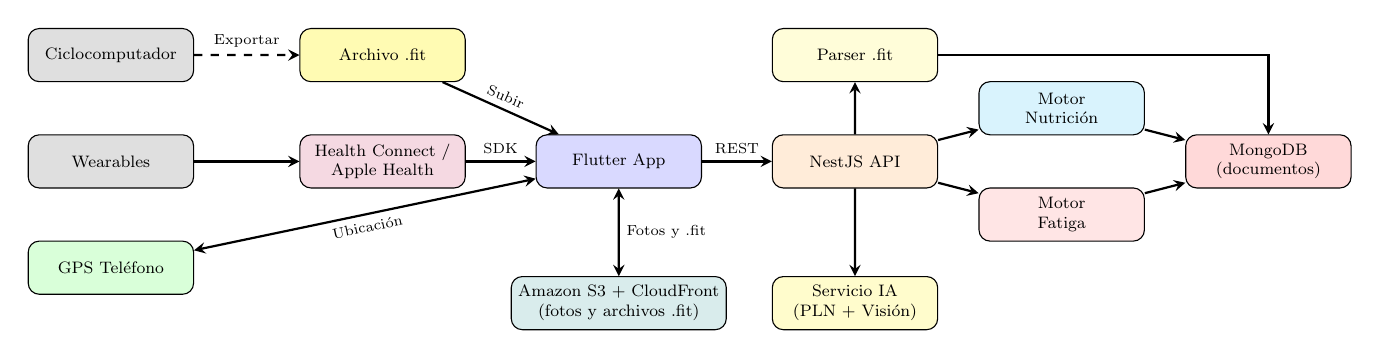
\begin{tikzpicture}[
    box/.style={draw, rectangle, rounded corners, minimum width=2.8cm, minimum height=0.9cm, fill=#1, align=center, font=\footnotesize},
    arrow/.style={->, thick, >=stealth},
    darrow/.style={<->, thick, >=stealth},
    dashed_arrow/.style={->, dashed, thick, >=stealth},
    lbl/.style={font=\scriptsize},
    scale=0.75, transform shape
]
    % Dispositivos del usuario
    \node (ciclo) [box=gray!25] at (-0.6,1.8) {Ciclocomputador};
    \node (wear) [box=gray!25] at (-0.6,0) {Wearables};
    \node (gps) [box=green!15] at (-0.6,-1.8) {GPS Teléfono};

    % Concentradores y archivo exportado
    \node (fit) [box=yellow!30] at (4,1.8) {Archivo .fit};
    \node (hc) [box=purple!15] at (4,0) {Health Connect /\\Apple Health};

    % Aplicación y almacenamiento de archivos
    \node (app) [box=blue!15] at (8,0) {Flutter App};
    \node (s3) [box=teal!15] at (8,-2.4) {Amazon S3 + CloudFront\\(fotos y archivos .fit)};

    % Backend
    \node (api) [box=orange!15] at (12,0) {NestJS API};
    \node (parser) [box=yellow!15] at (12,1.8) {Parser .fit};
    \node (ai) [box=yellow!20] at (12,-2.4) {Servicio IA\\(PLN + Visión)};
    \node (nutri) [box=cyan!15] at (15.5,0.9) {Motor\\Nutrición};
    \node (fatiga) [box=red!10] at (15.5,-0.9) {Motor\\Fatiga};

    % Base de datos
    \node (db) [box=red!15] at (19,0) {MongoDB\\(documentos)};

    % Flechas
    \draw[dashed_arrow] (ciclo) -- node[above, lbl] {Exportar} (fit);
    \draw[arrow] (wear) -- (hc);
    \draw[arrow] (fit) -- node[above, lbl, sloped] {Subir} (app);
    \draw[arrow] (hc) -- node[above, lbl] {SDK} (app);
    \draw[darrow] (gps) -- node[below, lbl, sloped] {Ubicación} (app);
    \draw[darrow] (app) -- node[right, lbl] {Fotos y .fit} (s3);
    \draw[arrow] (app) -- node[above, lbl] {REST} (api);
    \draw[arrow] (api) -- (parser);
    \draw[arrow] (api) -- (ai);
    \draw[arrow] (api) -- (nutri);
    \draw[arrow] (api) -- (fatiga);
    \draw[arrow] (nutri) -- (db);
    \draw[arrow] (fatiga) -- (db);
    \draw[arrow] (parser) -| (db);

\end{tikzpicture}
\captionof{figure}{Arquitectura técnica de la Solución (Alternativa 3).}
\label{fig:arquitectura_solucion}
\end{center}
\newpage
\subsubsection{Módulos Principales y Diagrama de Interacción}
El sistema se divide en módulos funcionales que se comunican entre sí:

\textbf{1. Módulo de Ingesta de Telemetría (El Núcleo de Entrada)}\\
Se encarga de que registrar datos sea lo más simple posible para el deportista, usando tres capas:
\begin{itemize}
    \item Capa Manual: El usuario ingresa sus rutinas (series, repeticiones y peso) o su RPE (percepción subjetiva del esfuerzo).
    \item Capa de Concentradores del SO: La aplicación se sincroniza en segundo plano con Health Connect o Apple Health para obtener datos generales (pasos, calorías activas y frecuencia cardíaca en reposo).
    \item Capa Avanzada (.fit): Para deportistas que usan dispositivos especializados (Garmin, Wahoo, Polar), la API recibe directamente archivos \texttt{.fit}. Un lector (parser) que invoca el backend decodifica el archivo y obtiene datos precisos segundo a segundo (potencia en ciclismo, zonas cardíacas y altimetría).
\end{itemize}

\textbf{2. Motor de Fatiga y Planificación (La Lógica de Negocio Central)}\\
Este módulo cruza los datos fisiológicos que entrega el módulo de ingesta. Al final del día, o después de cada entrenamiento, calcula la carga crónica (CTL) y la carga aguda (ATL). Si el usuario tiene mucha fatiga acumulada por una sesión de resistencia exigente y tiene programada una sesión de fuerza máxima al día siguiente, el sistema le enviará una sugerencia (mediante una notificación push) para que considere bajar el número de series o la carga, y así evitar la interferencia y el sobreentrenamiento. La decisión final queda en manos del usuario.

\textbf{3. Motor de Nutrición Asistida por IA}\\
Deja de lado las metas calóricas fijas y se ajusta según el motor de fatiga. Si el usuario hizo un entrenamiento largo y exigente, el módulo sugiere subir su meta diaria de carbohidratos y la muestra en la aplicación. Además, el usuario puede enviar fotos de sus comidas. NestJS manda la imagen, junto con instrucciones predefinidas (prompt), a la API de visión artificial y recibe una estimación de los macronutrientes. Si la IA tiene poca seguridad en su resultado, le pide al usuario que lo revise, para que los datos guardados sean confiables.
\newpage
\textbf{4. Red Social Deportiva}\\
Este módulo convierte la aplicación en una comunidad. Los usuarios pueden seguir a otras personas, ver un muro con sus publicaciones y publicar en su perfil sus sesiones de fuerza, sus rutas y sus comidas. Lo que lo diferencia es que lo publicado no queda solo como información para leer, sino que se puede usar. Por ejemplo, si un usuario publica su rutina de pecho, otro usuario puede agregarla con un botón a sus rutinas de fuerza, sin copiarla a mano. Lo mismo ocurre con una ruta, que pasa a su módulo de cardio, y con una receta, que pasa a su módulo de nutrición. En el caso de una receta como ``Panqueques Proteicos'', el sistema además ajusta las porciones y los gramos de cada ingrediente para que calcen con lo que ese usuario necesita. Todo lo agregado desde la comunidad entra al cruce de datos como cualquier otro registro. Las fotos de las publicaciones (hasta 4 por publicación) se suben desde el teléfono directamente a Amazon S3 con un permiso temporal que entrega este módulo, y se muestran a través de CloudFront.
\\\\
\textbf{5. Perfil del Usuario y Plan Sugerido}\\
Al registrarse, el usuario responde un cuestionario corto sobre su experiencia, sus objetivos, los días disponibles, su equipamiento, las disciplinas que practica y sus datos corporales básicos. Con eso, el sistema lo clasifica según su nivel (principiante, intermedio o avanzado) y su orientación (más fuerza, más resistencia o equilibrada), y le sugiere un plan semanal a partir de una plantilla para ese perfil. Después, el plan se ajusta con lo que el usuario registra. Si no cumple las sesiones, si reporta un esfuerzo muy alto o si el motor de fatiga detecta una carga excesiva, el sistema sugiere un plan más liviano, y si progresa bien, uno más exigente. El usuario siempre puede modificar o ignorar el plan.
\newpage
El siguiente diagrama muestra cómo se relacionan estos módulos. Las flechas que bajan desde la aplicación indican lo que el usuario envía a cada módulo y lo que recibe de vuelta. Las flechas dentro del backend muestran cómo un módulo usa los resultados de otro. Por ejemplo, la carga de cada sesión alimenta al motor de fatiga, y este ajusta el plan sugerido y las metas de nutrición. Las cajas con borde punteado son servicios externos.

\vspace{0.5cm}
\begin{center}
\setstretch{1}
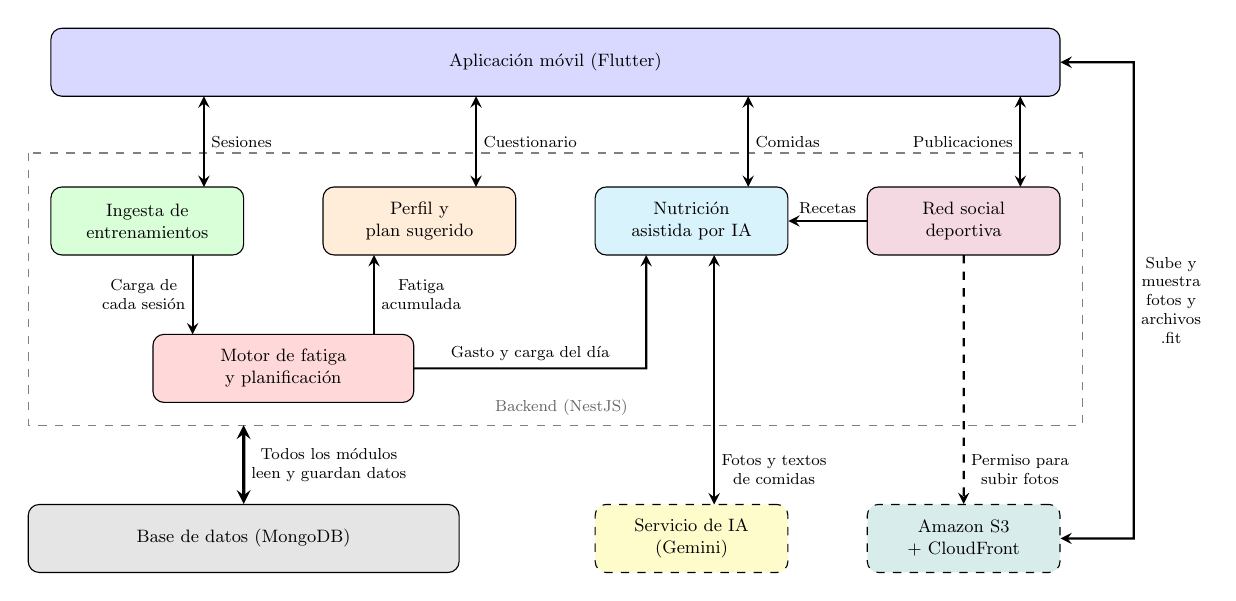
\begin{tikzpicture}[
    box/.style={draw, rectangle, rounded corners, minimum width=3.4cm, minimum height=1.2cm, fill=#1, align=center, font=\small},
    ext/.style={draw, dashed, rectangle, rounded corners, minimum width=3.4cm, minimum height=1.2cm, fill=#1, align=center, font=\small},
    lbl/.style={font=\footnotesize, align=center},
    arrow/.style={->, thick, >=stealth},
    darrow/.style={<->, thick, >=stealth},
    scale=0.72, transform shape
]
    % Aplicación móvil
    \node (ui) [box=blue!15, minimum width=17.8cm] at (7.2,0) {Aplicación móvil (Flutter)};

    % Módulos del backend
    \node (tel) [box=green!15] at (0,-2.8) {Ingesta de\\entrenamientos};
    \node (per) [box=orange!15] at (4.8,-2.8) {Perfil y\\plan sugerido};
    \node (nut) [box=cyan!15] at (9.6,-2.8) {Nutrición\\asistida por IA};
    \node (soc) [box=purple!15] at (14.4,-2.8) {Red social\\deportiva};
    \node (fat) [box=red!15, minimum width=4.6cm] at (2.4,-5.4) {Motor de fatiga\\y planificación};

    % Agrupación del backend
    \draw[dashed, gray] (-2.1,-1.6) rectangle (16.5,-6.4);
    \node[font=\footnotesize, text=gray!80!black, anchor=south east] at (8.6,-6.35) {Backend (NestJS)};

    % Servicios y almacenamiento
    \node (db) [box=gray!20, minimum width=7.6cm] at (1.7,-8.4) {Base de datos (MongoDB)};
    \node (ia) [ext=yellow!20] at (9.6,-8.4) {Servicio de IA\\(Gemini)};
    \node (s3) [ext=teal!15] at (14.4,-8.4) {Amazon S3\\+ CloudFront};

    % Aplicación hacia los módulos
    \draw[darrow] (1.0,-0.6) -- node[lbl, right] {Sesiones} (1.0,-2.2);
    \draw[darrow] (5.8,-0.6) -- node[lbl, right] {Cuestionario} (5.8,-2.2);
    \draw[darrow] (10.6,-0.6) -- node[lbl, right] {Comidas} (10.6,-2.2);
    \draw[darrow] (15.4,-0.6) -- node[lbl, left] {Publicaciones} (15.4,-2.2);

    % Cruces entre módulos
    \draw[arrow] (0.8,-3.4) -- node[lbl, left] {Carga de\\cada sesión} (0.8,-4.8);
    \draw[arrow] (4.0,-4.8) -- node[lbl, right] {Fatiga\\acumulada} (4.0,-3.4);
    \draw[arrow] (fat.east) -- node[lbl, above] {Gasto y carga del día} (8.8,-5.4) -- (8.8,-3.4);
    \draw[arrow] (soc.west) -- node[lbl, above] {Recetas} (nut.east);

    % Hacia servicios externos y datos
    \draw[darrow] (10.0,-3.4) -- node[lbl, right, pos=0.86] {Fotos y textos\\de comidas} (10.0,-7.8);
    \draw[arrow, dashed] (14.4,-3.4) -- node[lbl, right, pos=0.86] {Permiso para\\subir fotos} (s3.north);
    \draw[darrow] (ui.east) -- (17.4,0) -- node[lbl, right] {Sube y\\muestra\\fotos y\\archivos\\.fit} (17.4,-8.4) -- (s3.east);
    \draw[darrow, very thick] (1.7,-6.4) -- node[lbl, right] {Todos los módulos\\leen y guardan datos} (db.north);
\end{tikzpicture}
\captionof{figure}{Diagrama de Interacción entre módulos funcionales.}
\label{fig:interaccion_modulos}
\end{center}
\newpage
\subsubsection{Modelo de Datos (Esquema Conceptual)}
Como los datos del sistema son de tipos muy distintos, la base de datos MongoDB se organizará en colecciones de documentos. Las colecciones principales serán:
\begin{itemize}
    \item \textbf{users (Usuarios):} Guarda las credenciales del usuario y, dentro del mismo documento, su perfil físico, sus metas y los tokens de acceso a servicios de terceros.
    \item \textbf{dailyLogs (Registro Diario):} Un documento por usuario y fecha. Contiene las metas calóricas del día, que se calculan a partir de lo que entrega el motor de fatiga, y los reportes de sensaciones.
    \item \textbf{workouts (Entrenamientos):} Guarda tanto las sesiones de fuerza como las de cardio, diferenciadas por un campo de tipo. En las de fuerza, los ejercicios y las series van dentro del mismo documento.
    \item \textbf{telemetry (Telemetría):} Colección de series temporales que guarda los datos segundo a segundo de potencia y pulsaciones que llegan desde la capa avanzada.
    \item \textbf{posts y follows (Red Social):} Guardan las publicaciones de cada usuario (sesiones, rutas o comidas) y las relaciones entre seguidores. Las fotos de cada publicación no se guardan aquí, solo su dirección en Amazon S3.
    \item \textbf{trainingPlans (Plan Sugerido):} Guarda el plan semanal sugerido de cada usuario, junto con el perfil que se usó para generarlo.
    \item \textbf{meals (Comidas):} Registro de alimentación con sus alimentos dentro del documento. Si se registró con visión artificial, incluye un campo \texttt{aiConfidenceScore} que indica qué tan segura estaba la IA de su estimación.
\end{itemize}
\newpage
\subsubsection{Requerimientos de Infraestructura y Despliegue}
Para ponerla en marcha, la API de NestJS se empaquetará en contenedores \textbf{Docker}. Así, el entorno de desarrollo y el de producción son iguales. La imagen se desplegará en AWS Fargate, el servicio usado en la estimación de costos, que agrega más capacidad automáticamente cuando aumentan las peticiones, por ejemplo cuando muchos usuarios sincronizan sus dispositivos al mismo tiempo.
\\\\
La base de datos se alojará en MongoDB Atlas, el servicio administrado de MongoDB, que hace respaldos automáticos, permite recuperar los datos y cifra el almacenamiento, cumpliendo con los requisitos de ciberseguridad descritos en la factibilidad operativa.
\\\\
Las fotos y los archivos \texttt{.fit} se guardarán en un bucket privado de Amazon S3 en la región de São Paulo, con cifrado activado y una regla que borra los archivos que ya no se usan. Las fotos se mostrarán a través de Amazon CloudFront, que es el único servicio con permiso para leer ese bucket.
\newpage
\subsection{Beneficios del Proyecto}
La plataforma basada en la Alternativa 3 (Solución por Capas) trae varios beneficios, que se pueden separar entre los beneficios para el usuario (el atleta híbrido) y los beneficios comerciales del proyecto.

\textbf{Beneficios para el Usuario (Atleta Híbrido):}
\begin{itemize}
    \item \textbf{Todo en un solo lugar:} El atleta ya no necesita cambiar entre tres aplicaciones distintas (registro de pesas, registro con GPS y contador de calorías). Toda su información deportiva queda en un único panel.
    \item \textbf{Prevención del sobreentrenamiento (fatiga cruzada):} Al cruzar la carga reciente de resistencia con los entrenamientos de fuerza, el sistema avisa al usuario cuando su cuerpo no se ha recuperado y le sugiere bajar las cargas del gimnasio, ayudando a prevenir lesiones y estancamientos.
    \item \textbf{Nutrición ajustada al entrenamiento:} En vez de seguir una meta calórica fija, el atleta recibe sugerencias para tener suficiente glucógeno en los días de resistencia larga y suficiente proteína para recuperar el músculo.
    \item \textbf{Red social con contenido reutilizable:} El usuario puede seguir a otras personas y agregar sus sesiones, rutas y recetas a sus propios módulos con un botón, sin copiar nada a mano. Las recetas se adaptan automáticamente a sus necesidades del día.
    \item \textbf{Plan personalizado:} Incluso sin experiencia previa, el usuario recibe un plan semanal sugerido según su nivel y sus objetivos, que se ajusta con lo que registra.
\end{itemize}
\newpage
\textbf{Beneficios Comerciales y Operativos:}
\begin{itemize}
    \item \textbf{Modelo SaaS escalable:} Como se basa en infraestructura en la nube y en procesamiento automático con IA, el costo de sumar un nuevo suscriptor es muy bajo.
    \item \textbf{Historial acumulado:} A medida que el usuario acumula datos históricos de sus entrenamientos, le resulta menos conveniente cambiarse a otra aplicación o volver al registro manual, lo que favorece que siga usando la plataforma.
    \item \textbf{Ingresos directos:} Los atletas híbridos suelen estar dispuestos a pagar por herramientas que mejoren su rendimiento, lo que facilita conseguir usuarios premium.
\end{itemize}
\newpage
\subsection{Análisis Costo - Beneficio}
El análisis costo-beneficio compara la inversión necesaria para poner en marcha la Solución por Capas con los ingresos y beneficios esperados en un horizonte de 4 años.

\textbf{Estructura de Costos:}
\begin{itemize}
    \item \textbf{Inversión inicial (CAPEX):} Según la factibilidad económica, desarrollar la arquitectura completa (IA, lectura de archivos \texttt{.fit}, backend en NestJS y aplicación en Flutter) requiere una inversión inicial de \$16.230.402 CLP, que corresponde principalmente a horas de desarrollo y a la publicación en las tiendas.
    \item \textbf{Costos operativos anuales (OPEX):} La infraestructura en la nube, el almacenamiento de imágenes, el uso de APIs de IA, el mantenimiento y las licencias se estiman en \$4.543.368 CLP al año, a los que se suman \$601.879 CLP al año de impuesto a la renta. A esto se suman de forma indirecta el Costo de Adquisición de Clientes (CAC) y los gastos de marketing.
\end{itemize}

\textbf{Estructura de Beneficios:}
\begin{itemize}
    \item \textbf{Ingresos recurrentes mensuales (MRR):} La plataforma se financiará con una suscripción premium de \$7.990 CLP al mes.
    \item \textbf{Punto de equilibrio (Break-Even):} Los cálculos financieros mostraron que, para cubrir la inversión inicial y los costos operativos (con un VAN de 0 y una TIR del 15\%), el proyecto necesita mantener en promedio \textbf{159 suscriptores al año} durante 4 años, considerando el IVA, la comisión de las tiendas y el impuesto a la renta.
\end{itemize}

\textbf{Conclusión del Análisis:}\\
La relación costo-beneficio es \textbf{favorable}. Aunque el proyecto requiere un esfuerzo de desarrollo importante y es la alternativa más cara, necesitar 159 suscriptores es poco en comparación con el tamaño del mercado. Reunir en un solo lugar los datos de los dispositivos y las funciones de inteligencia artificial le da a la plataforma una ventaja clara frente a las aplicaciones aisladas, lo que justifica la inversión. Con esto se cierra el análisis de factibilidad y la definición de la arquitectura.

\newpage

% Ingeniería de Requerimientos
% Este archivo se incluye desde main.tex con \input.
\section{Ingeniería de Requerimientos}
\subsection{Introducción del Capítulo}
En el presente capítulo se aborda la fase de Ingeniería de Requerimientos, un paso fundamental para traducir las necesidades de los atletas híbridos en especificaciones técnicas claras y medibles. A partir del análisis metodológico y de las alternativas evaluadas previamente, aquí se define el comportamiento esperado del sistema, la interacción de sus procesos principales y las restricciones bajo las cuales debe operar. En primer lugar, se presentará el Modelo de Negocios enfocado en los procesos operativos core de la plataforma, seguido por el modelo detallado de requerimientos funcionales y no funcionales, para finalmente establecer los Casos de Uso que guiarán la construcción de la arquitectura de software.

\subsection{Modelo de Negocios (Procesos Core)}
En este capítulo, el modelo de negocios no se refiere a cómo gana dinero el proyecto, porque eso ya se analizó en la factibilidad económica del capítulo anterior. Aquí se refiere a los procesos principales que entregan valor al atleta. Se describen cinco procesos, y entre ellos cubren el registro de fuerza, de cardio y de comidas, el cruce de datos, la red social y el plan sugerido.
\\\\
Los procesos se dibujan con carriles, al estilo de BPMN (Business Process Model and Notation). Cada carril representa a un participante, el círculo simple marca el inicio, el círculo doble marca el fin y los rombos marcan las decisiones. Las tareas están numeradas, y después de cada diagrama se explica qué ocurre en cada una.
\newpage
\subsubsection{Proceso 1: Registro de Cardio y Cálculo de Fatiga Cruzada}
Este proceso muestra cómo una sesión de cardio entra a la aplicación, venga de donde venga, y cómo se cruza con el resto de los datos para avisar al atleta si está acumulando demasiada fatiga. Los participantes son el atleta, la aplicación y el reloj junto con la app de salud del teléfono. Responde a los requerimientos R02 y R03.

\begin{figure}[h!]
    \centering
    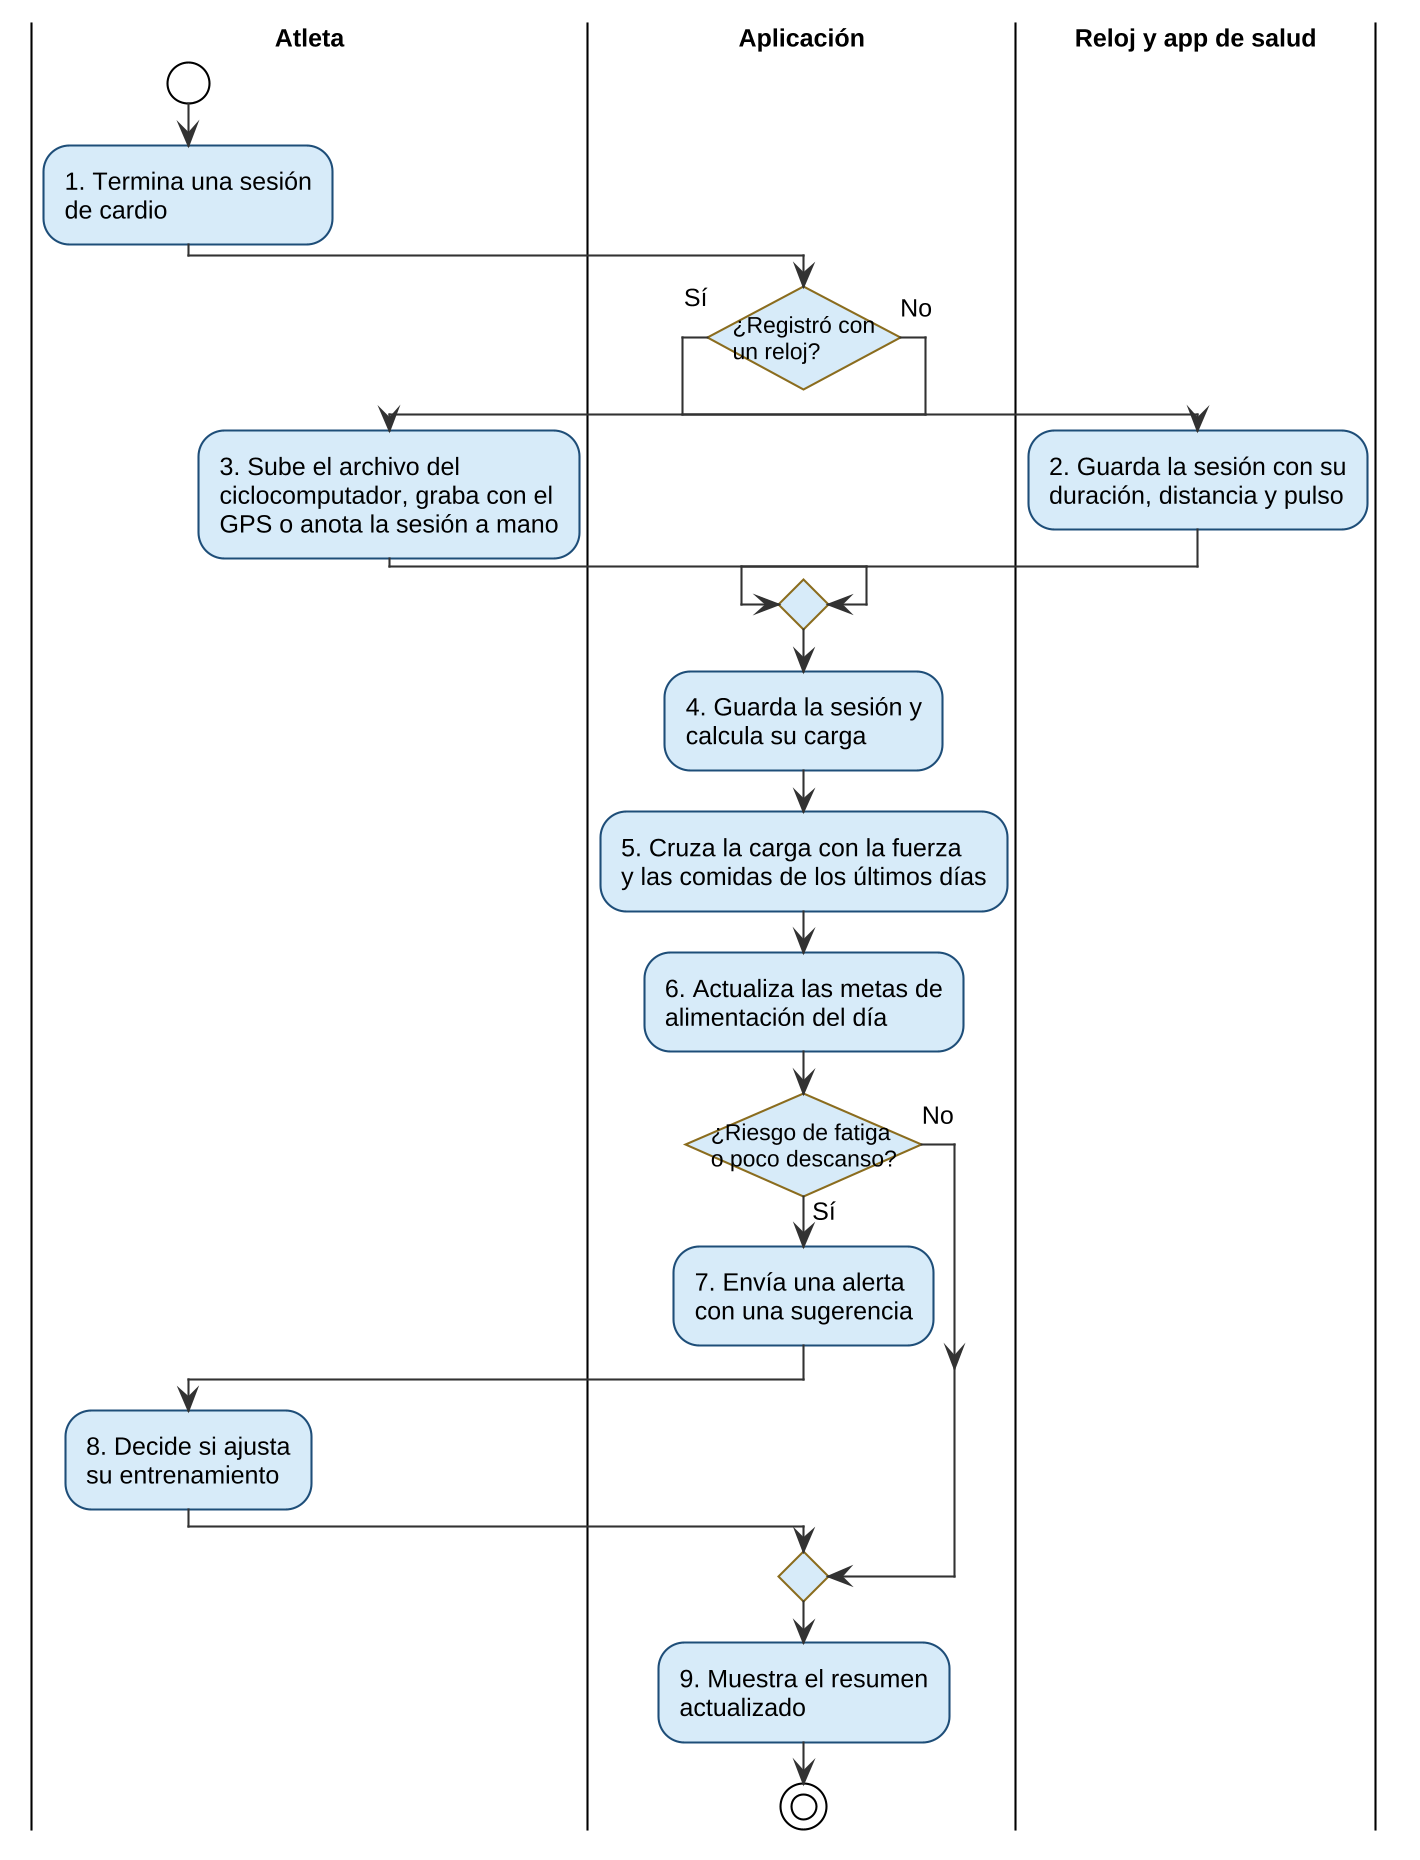
\includegraphics[width=0.68\textwidth]{figuras/procesos/bpmn_proceso1.png}
    \caption{Proceso 1: Registro de cardio y cálculo de fatiga cruzada.}
    \label{fig:bpmn_fatiga}
\end{figure}
\newpage
\textbf{Tareas del proceso}

\begin{enumerate}
    \item \textbf{Termina una sesión de cardio:} El proceso parte cuando el atleta termina una salida de ciclismo, running o trekking.
    \item \textbf{Guarda la sesión:} Si entrenó con un reloj, este guarda la sesión en Health Connect o Apple Salud. La aplicación la trae sola, siempre que el atleta haya dado permiso para leer esos datos.
    \item \textbf{Sube el archivo, graba o anota:} Si no usó un reloj, el atleta tiene tres opciones. Puede subir el archivo \texttt{.fit} de su ciclocomputador, grabar la ruta con el GPS del teléfono o anotar la sesión a mano. En las dos últimas también indica qué tan duro la sintió (RPE).
    \item \textbf{Guarda la sesión y calcula su carga:} La carga se calcula según la disciplina y los datos disponibles, como la potencia en ciclismo, el ritmo en running y el desnivel en trekking. Si faltan esos datos, se usan el pulso o el RPE. Si la misma sesión llega por dos vías, se usa la que tiene más detalle.
    \item \textbf{Cruza la carga:} La aplicación junta esta carga con las sesiones de fuerza y las comidas de los últimos días para estimar la fatiga cruzada. También revisa cuánto tiempo pasó entre sesiones de distinto tipo.
    \item \textbf{Actualiza las metas de alimentación:} Las metas del día cambian según lo entrenado, por ejemplo con más carbohidratos después de una salida larga. Son sugerencias y no una dieta.
    \item \textbf{Envía una alerta:} Si el atleta tiene mucha fatiga y una sesión exigente de la otra disciplina en las próximas 24 horas, o si dejó menos de 6 horas entre una sesión de fuerza y una de cardio, la aplicación le avisa y le sugiere, por ejemplo, bajar la carga o mover la sesión. Si además viene comiendo bastante menos de lo que gasta, el aviso también lo menciona.
    \item \textbf{Decide si ajusta su entrenamiento:} La aplicación no cambia nada por su cuenta. La decisión siempre es del atleta.
    \item \textbf{Muestra el resumen actualizado:} El atleta ve la sesión en su historial, junto con su carga acumulada.
\end{enumerate}

El plan gratuito llega hasta el registro con GPS o a mano. La lectura desde el reloj, el archivo \texttt{.fit}, el cruce de datos, las metas y las alertas son parte del plan premium.
\newpage
\subsubsection{Proceso 2: Registro de Comidas y Metas de Alimentación}
Este proceso muestra las cuatro formas de registrar una comida y cómo cada una se compara con las metas del día. Los participantes son el atleta, la aplicación y el asistente de inteligencia artificial. Responde a los requerimientos R04 y R05.

\begin{figure}[h!]
    \centering
    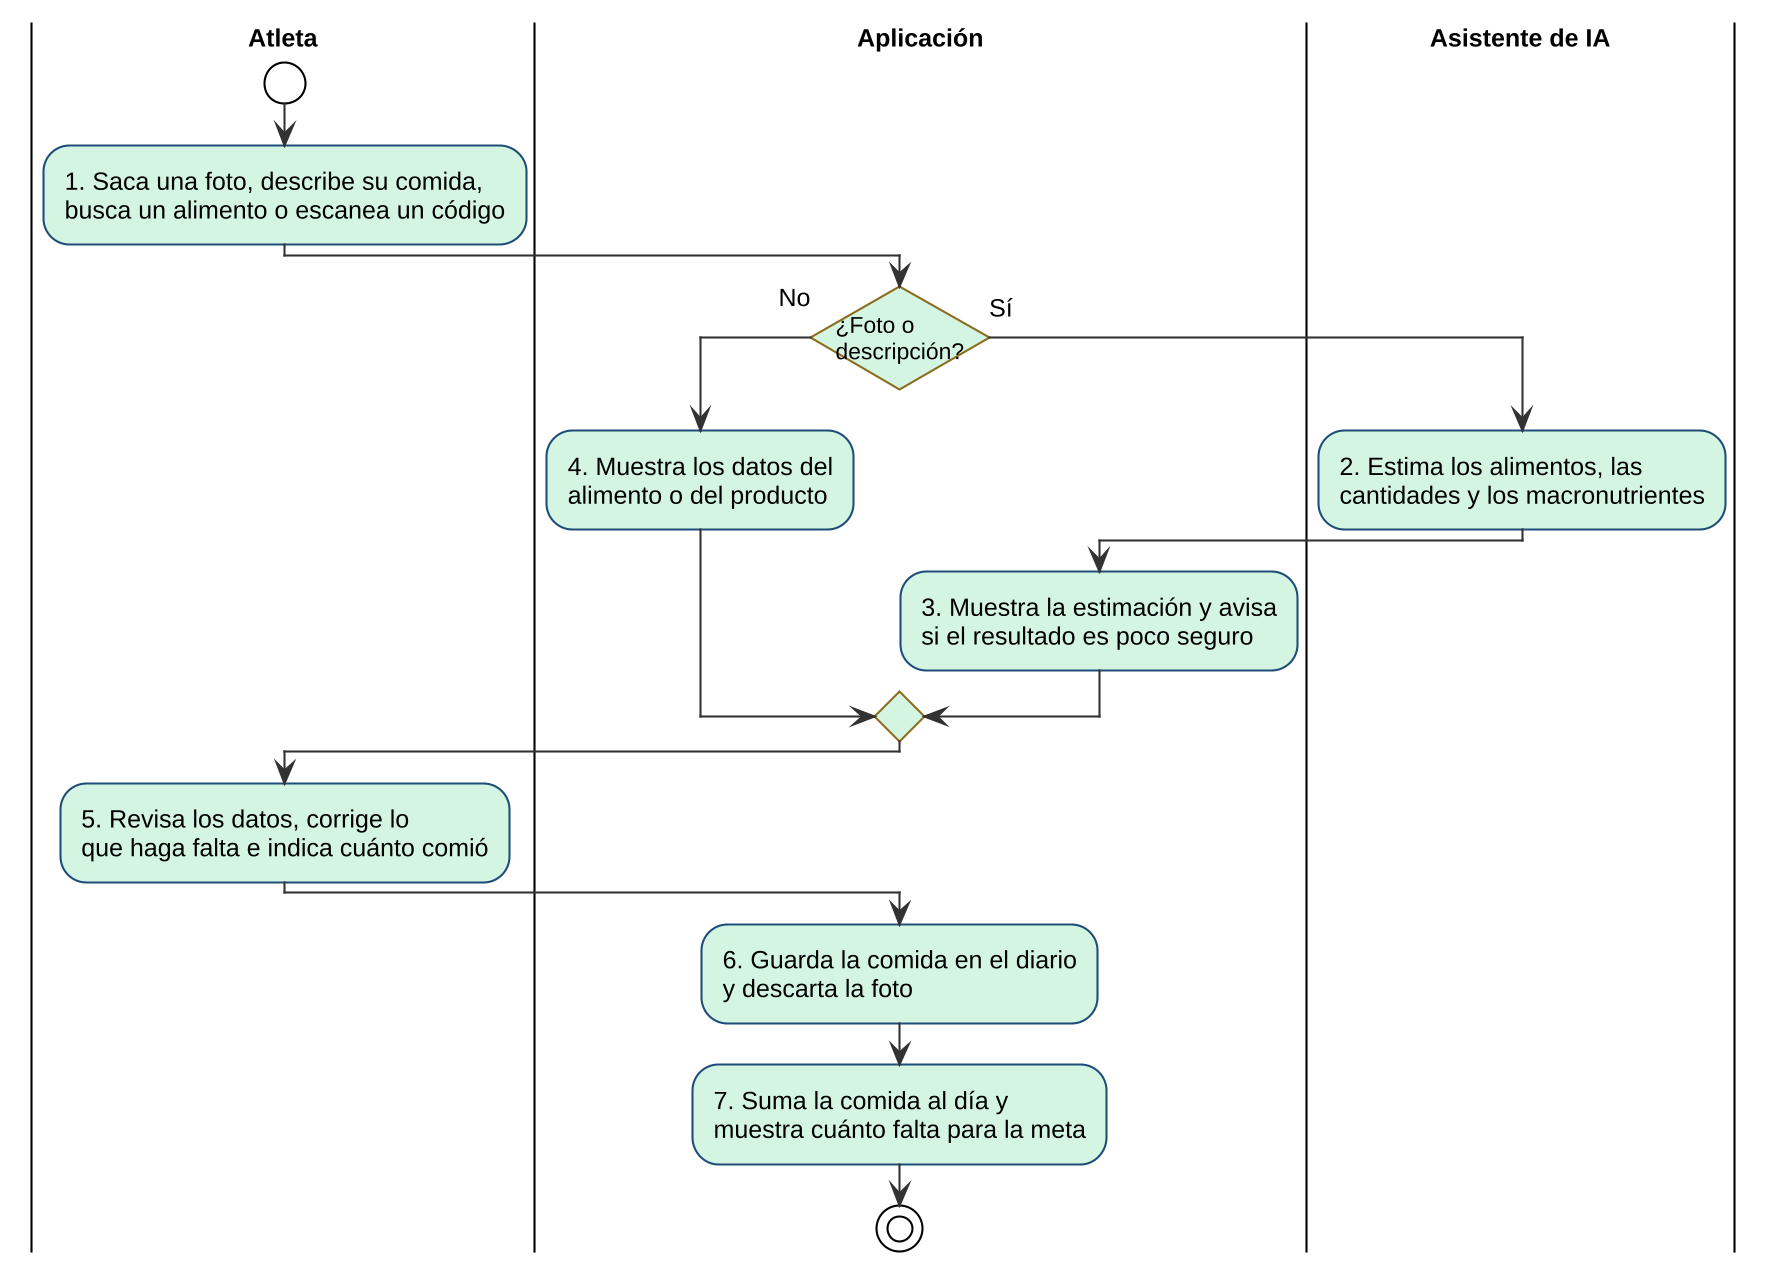
\includegraphics[width=0.9\textwidth]{figuras/procesos/bpmn_proceso2.png}
    \caption{Proceso 2: Registro de comidas y metas de alimentación.}
    \label{fig:bpmn_nutricion}
\end{figure}

\textbf{Tareas del proceso}

\begin{enumerate}
    \item \textbf{Elige cómo registrar:} El atleta saca una foto a su plato, describe su comida con sus palabras, busca un alimento en la lista o escanea el código de barras de un producto.
    \item \textbf{Estima la comida:} Si usó una foto o una descripción, el asistente de IA estima los alimentos, las cantidades, las calorías y los macronutrientes.
    \item \textbf{Muestra la estimación:} La aplicación muestra el resultado y avisa cuando es poco seguro, para que el atleta lo revise con más cuidado.
    \item \textbf{Muestra los datos del alimento:} Si buscó un alimento o escaneó un código, la aplicación muestra sus calorías y macronutrientes.
    \item \textbf{Revisa y corrige:} En todos los casos el atleta revisa los datos, corrige lo que haga falta e indica cuánto comió. Nada se guarda sin que lo confirme.
    \item \textbf{Guarda la comida:} La comida queda en el diario del día. La foto se descarta después del análisis, salvo que el atleta la quiera publicar.
    \item \textbf{Muestra el avance:} La aplicación suma la comida al día y muestra cuánto falta para las metas calculadas en el Proceso 1. También puede sugerir en qué momento conviene comer, por ejemplo proteína después de una sesión de fuerza.
\end{enumerate}

La búsqueda en la lista y el código de barras son parte del plan gratuito. La foto, la descripción y las metas según el entrenamiento son parte del plan premium.
\newpage
\subsubsection{Proceso 3: Publicación y Uso de Contenido de la Comunidad}
Este proceso muestra cómo una sesión, una ruta o una comida que publica un atleta llega a otro, que puede agregarla a sus propios módulos o reportarla. Los participantes son el atleta que publica, el atleta que ve la publicación, la aplicación y el administrador. Responde a los requerimientos R08, R11 y R12.

\begin{figure}[h!]
    \centering
    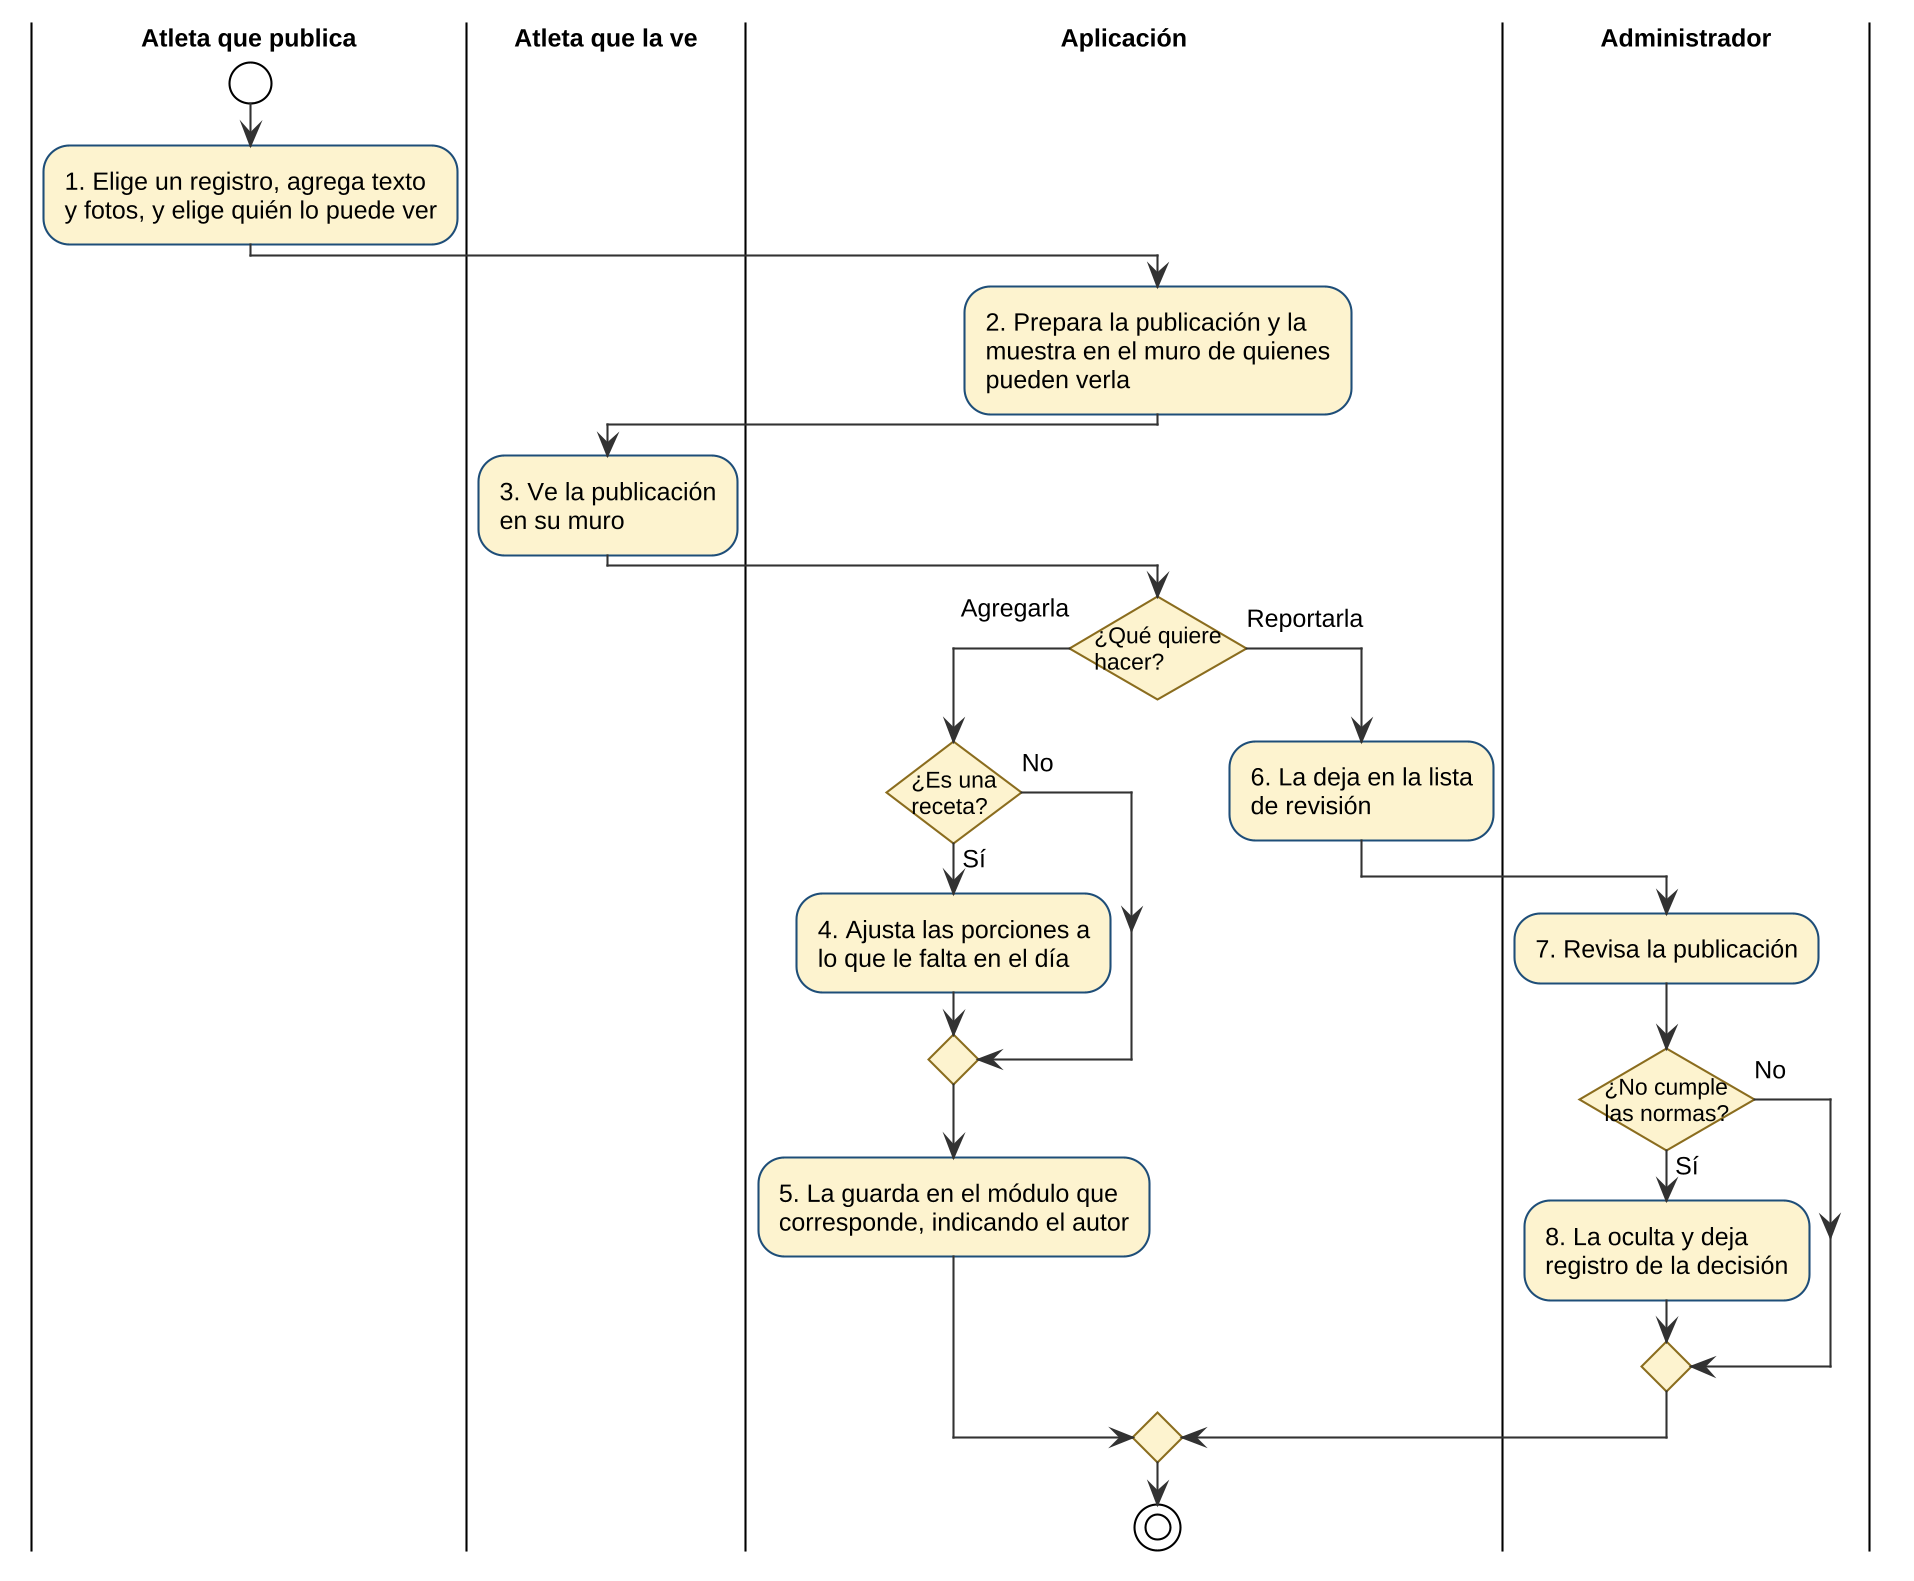
\includegraphics[width=0.85\textwidth]{figuras/procesos/bpmn_proceso3.png}
    \caption{Proceso 3: Publicación y uso de contenido de la comunidad.}
    \label{fig:bpmn_recetas}
\end{figure}
\newpage
\textbf{Tareas del proceso}

\begin{enumerate}
    \item \textbf{Publica un registro:} El atleta elige una sesión, una ruta o una comida que ya registró, le agrega un texto y hasta 4 fotos, y elige quién la puede ver (todos, sus seguidores o solo él).
    \item \textbf{Prepara y muestra la publicación:} La aplicación comprime las fotos, les borra los datos de ubicación y, si es una ruta, oculta el inicio y el final del recorrido. Luego la publicación aparece en el muro de quienes pueden verla.
    \item \textbf{Ve la publicación:} Otro atleta la encuentra en su muro. Si le interesa, puede agregarla a sus módulos o reportarla.
    \item \textbf{Ajusta las porciones:} Si agrega una receta, la aplicación ajusta la cantidad de cada ingrediente según lo que le falta comer ese día, manteniendo las proporciones de la receta original.
    \item \textbf{Guarda en el módulo que corresponde:} Una sesión de fuerza queda como rutina, una ruta queda en cardio y una receta queda en nutrición, siempre indicando quién la creó. Agregar una receta no la registra como comida. Eso ocurre cuando el atleta se la come y la anota en su diario (Proceso 2).
    \item \textbf{Deja la publicación en revisión:} Si el atleta la reporta, indica el motivo y la publicación pasa a la lista de revisión del administrador.
    \item \textbf{Revisa la publicación:} El administrador evalúa si cumple las normas de la comunidad o si puede ser peligrosa para la salud.
    \item \textbf{Oculta la publicación:} Si no cumple las normas, el administrador la oculta y queda registro de quién tomó la decisión y por qué.
\end{enumerate}
\newpage
\subsubsection{Proceso 4: Registro de Fuerza}
Este proceso muestra las dos formas de registrar una sesión de fuerza, ya sea con el formulario o con las propias palabras del atleta, para que anotar una sesión tome poco tiempo. Los participantes son el atleta, la aplicación y el asistente de inteligencia artificial. Responde al requerimiento R01.

\begin{figure}[h!]
    \centering
    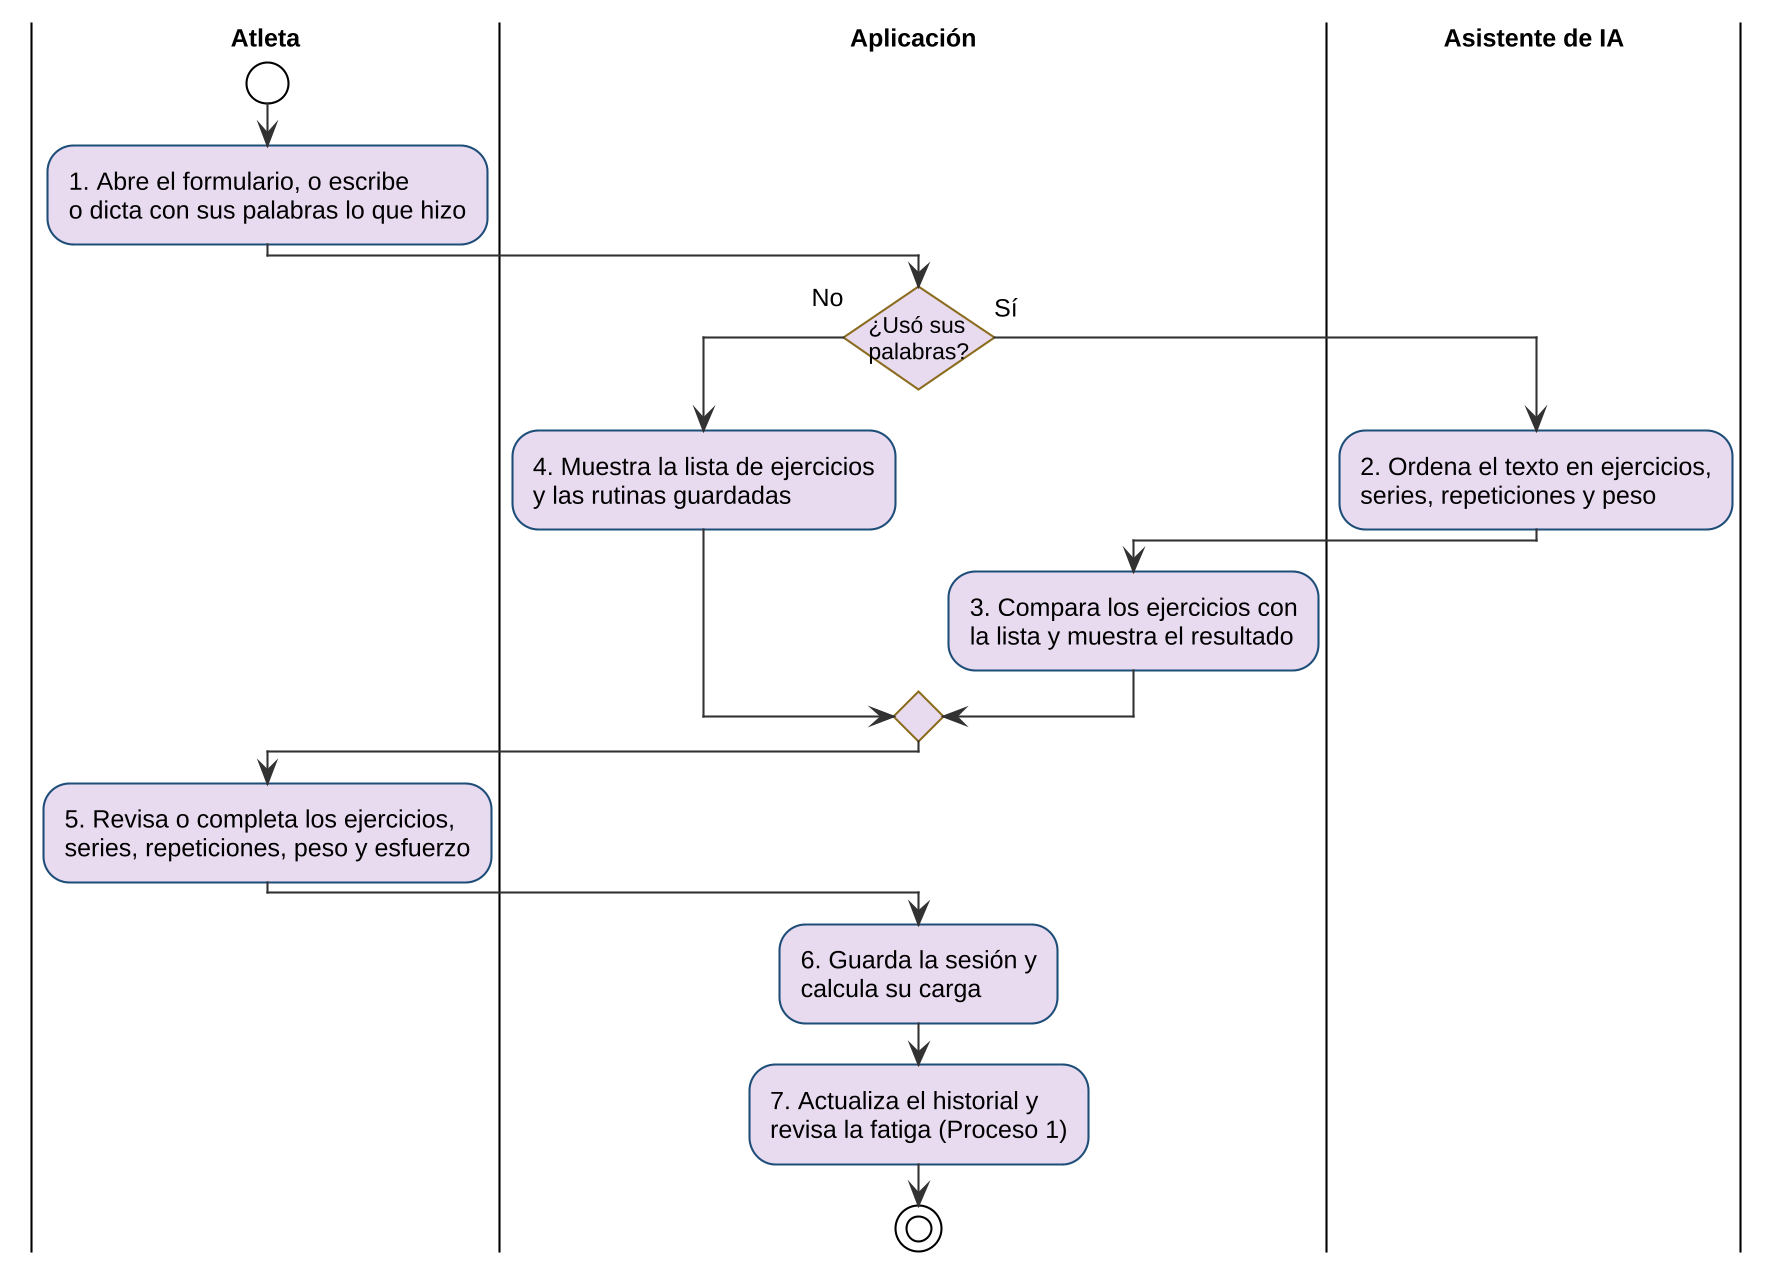
\includegraphics[width=0.9\textwidth]{figuras/procesos/bpmn_proceso4.png}
    \caption{Proceso 4: Registro de fuerza.}
    \label{fig:bpmn_nlp}
\end{figure}

\textbf{Tareas del proceso}

\begin{enumerate}
    \item \textbf{Elige cómo registrar:} El atleta abre el formulario, o escribe o dicta lo que hizo, por ejemplo ``hice 4 series de 8 sentadillas con 100 kilos''.
    \item \textbf{Ordena el texto:} Si usó sus palabras, el asistente de IA separa el texto en ejercicios, series, repeticiones y peso.
    \item \textbf{Compara con la lista:} La aplicación busca cada ejercicio en su lista y muestra el resultado.
    \item \textbf{Muestra la lista y las rutinas:} Si usó el formulario, la aplicación muestra la lista de ejercicios y las rutinas que el atleta tiene guardadas.
    \item \textbf{Revisa o completa:} El atleta confirma o completa los ejercicios, las series, las repeticiones, el peso y qué tan duro lo sintió (RPE). Nada se guarda sin que lo confirme.
    \item \textbf{Guarda la sesión:} La aplicación guarda la sesión y calcula su carga.
    \item \textbf{Actualiza el historial y revisa la fatiga:} La sesión aparece en el historial. Con esta carga se repite el cruce de datos desde la tarea 5 del Proceso 1, de modo que una sesión de fuerza también puede generar una alerta antes de una sesión exigente de cardio.
\end{enumerate}

El formulario es parte del plan gratuito. El registro con las propias palabras y el cruce de datos son parte del plan premium.
\newpage
\subsubsection{Proceso 5: Perfil del Usuario y Plan Sugerido}
Este proceso muestra cómo la aplicación conoce a un usuario nuevo, le sugiere un plan de entrenamiento y lo va ajustando cada semana con lo que registra. Es el proceso que da una guía a quien recién empieza. Los participantes son el atleta y la aplicación. Responde al requerimiento R13.

\begin{figure}[h!]
    \centering
    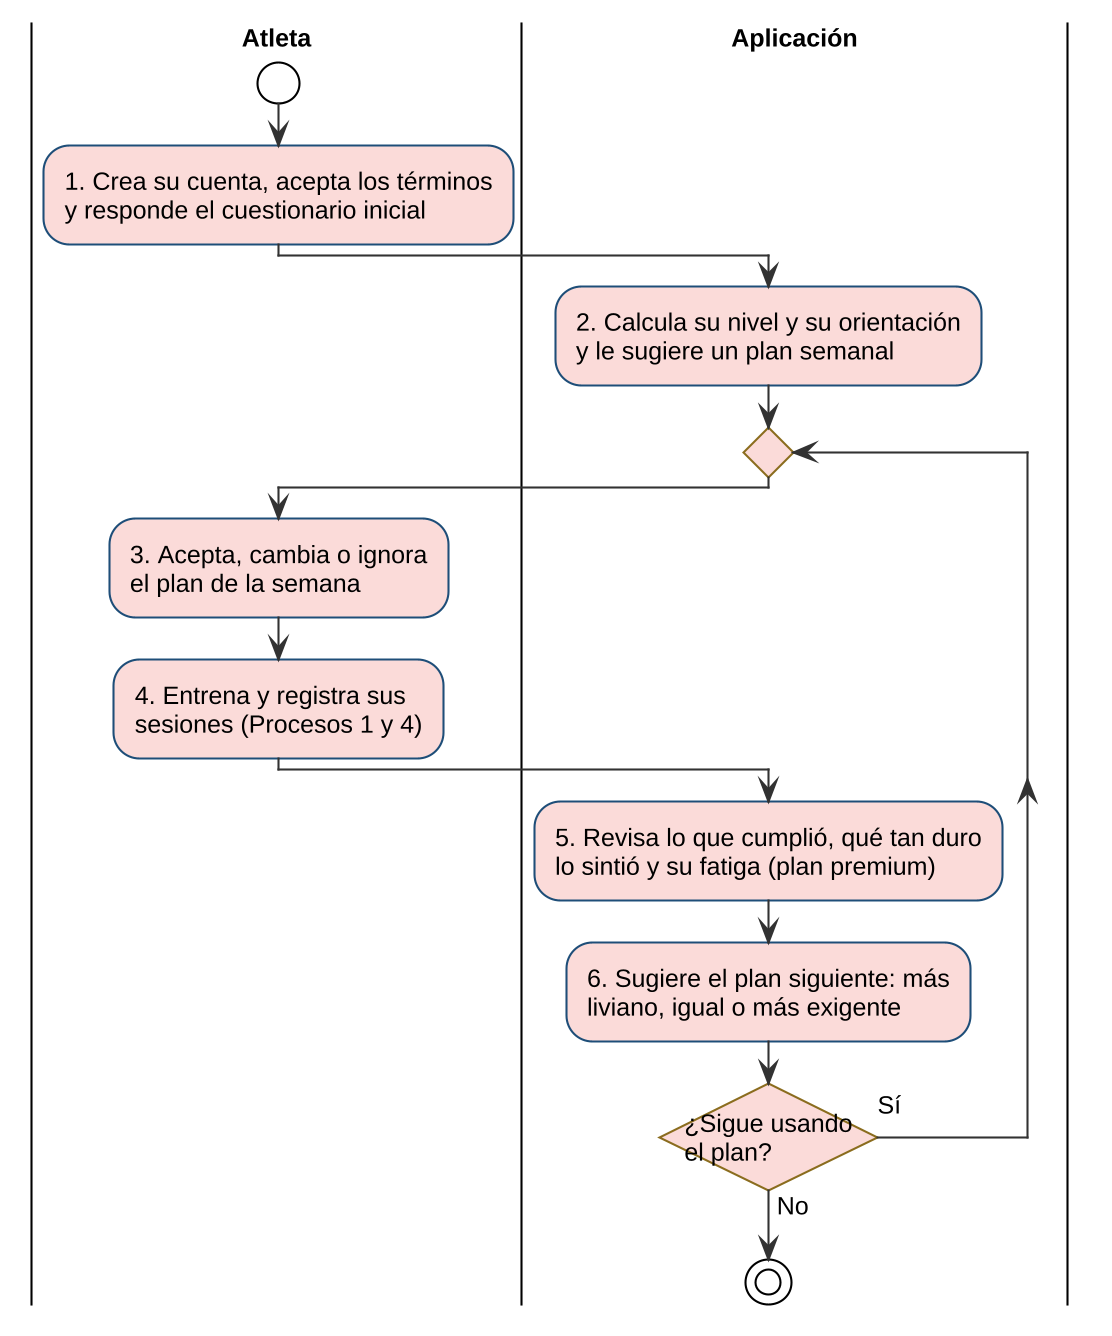
\includegraphics[width=0.62\textwidth]{figuras/procesos/bpmn_proceso5.png}
    \caption{Proceso 5: Perfil del usuario y plan sugerido.}
    \label{fig:bpmn_plan}
\end{figure}

\textbf{Tareas del proceso}

\begin{enumerate}
    \item \textbf{Crea su cuenta y responde el cuestionario:} El atleta acepta los términos de uso y el aviso legal, y responde preguntas sobre su experiencia, sus objetivos, los días que puede entrenar, su equipamiento, las disciplinas que practica, su edad, su sexo, su estatura y su peso.
    \item \textbf{Calcula su nivel y sugiere un plan:} La aplicación lo clasifica según su nivel (principiante, intermedio o avanzado) y su orientación (más fuerza, más resistencia o equilibrada), y le sugiere un plan semanal a partir de una plantilla para ese perfil.
    \item \textbf{Acepta, cambia o ignora el plan:} El plan es una sugerencia, y la decisión siempre es del atleta.
    \item \textbf{Entrena y registra:} Durante la semana registra sus sesiones, como se explica en los Procesos 1 y 4.
    \item \textbf{Revisa la semana:} La aplicación compara las sesiones cumplidas con las sugeridas y revisa qué tan duro las sintió el atleta. En el plan premium también considera su fatiga cruzada.
    \item \textbf{Sugiere el plan siguiente:} Con reglas simples, la aplicación propone un plan más liviano, igual o más exigente, y explica por qué cambió. El ciclo se repite cada semana mientras el atleta siga usando el plan.
\end{enumerate}
\newpage
\subsection{Modelo de Requerimientos}
El Modelo de Requerimientos reúne lo que el sistema debe hacer de cara al usuario (requerimientos funcionales) y la forma técnica en que se va a lograr (requerimientos no funcionales). A continuación se presenta el diagrama de trazabilidad, que relaciona los procesos de negocio de la sección anterior (cardio y fatiga, comidas y metas, comunidad, registro de fuerza y plan sugerido) con los requerimientos funcionales que los hacen posibles. Los requerimientos que no pertenecen a un proceso en particular se agrupan como funciones transversales de la plataforma.

\begin{figure}[h!]
    \centering
    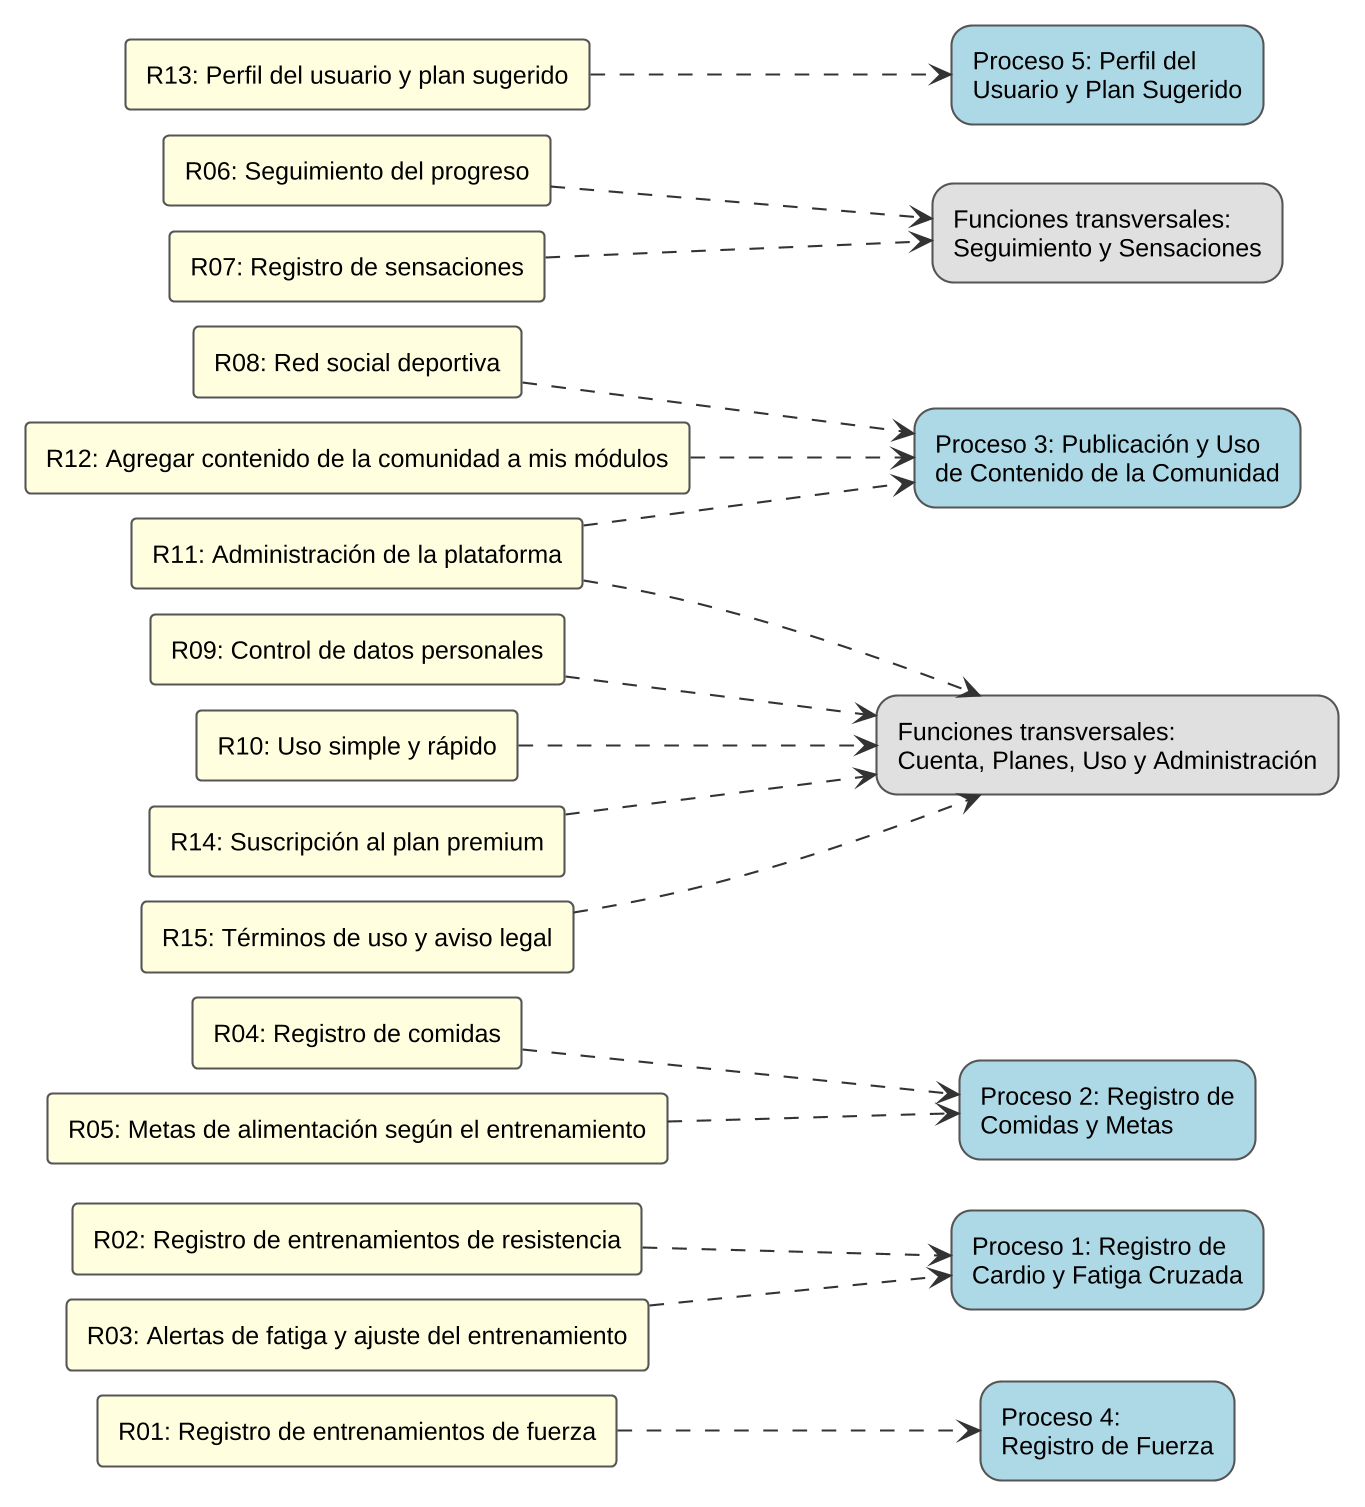
\includegraphics[width=0.8\textwidth]{figuras/requerimientos/diagrama_requerimientos.png}
    \caption{Diagrama de trazabilidad: relación entre requerimientos y procesos de negocio.}
    \label{fig:diagrama_requerimientos}
\end{figure}
\newpage
\subsubsection{Requerimientos Funcionales}
Los requerimientos funcionales describen lo que la aplicación permite hacer al usuario y lo que le entrega a cambio. Se presentan en quince requerimientos, escritos desde el punto de vista de quien usa la aplicación y no de los procesos internos del sistema. Catorce corresponden al deportista y uno al administrador de la plataforma.

\begin{table}[h!]
    \centering
    \renewcommand{\arraystretch}{1.3}
    \begin{tabular}{|p{3.5cm}|p{11.5cm}|}
        \hline
        \rowcolor[HTML]{EFEFEF} 
        \textbf{Identificador} & \textbf{R01} \\ \hline
        \textbf{Nombre} & Registro de entrenamientos de fuerza \\ \hline
        \textbf{Descripción} & La aplicación debe permitir al usuario registrar sus sesiones de fuerza. Puede elegir los ejercicios desde un catálogo e ingresar las series, repeticiones, peso y esfuerzo percibido (RPE), o describir la sesión con sus propias palabras, escribiéndola o dictándola. \\ \hline
        \textbf{Prioridad} & Alta \\ \hline
    \end{tabular}
\end{table}

\begin{table}[h!]
    \centering
    \renewcommand{\arraystretch}{1.3}
    \begin{tabular}{|p{3.5cm}|p{11.5cm}|}
        \hline
        \rowcolor[HTML]{EFEFEF} 
        \textbf{Identificador} & \textbf{R02} \\ \hline
        \textbf{Nombre} & Registro de entrenamientos de resistencia \\ \hline
        \textbf{Descripción} & La aplicación debe permitir al usuario registrar sus sesiones de ciclismo, running y trekking. Los datos pueden provenir del GPS del teléfono, de su reloj o ciclocomputador, o de un archivo exportado desde estos dispositivos. Si no cuenta con datos de un dispositivo, puede registrar la sesión indicando cómo sintió el esfuerzo. \\ \hline
        \textbf{Prioridad} & Alta \\ \hline
    \end{tabular}
\end{table}

\begin{table}[h!]
    \centering
    \renewcommand{\arraystretch}{1.3}
    \begin{tabular}{|p{3.5cm}|p{11.5cm}|}
        \hline
        \rowcolor[HTML]{EFEFEF} 
        \textbf{Identificador} & \textbf{R03} \\ \hline
        \textbf{Nombre} & Alertas de fatiga y ajuste del entrenamiento \\ \hline
        \textbf{Descripción} & La aplicación debe cruzar las métricas de esfuerzo de las sesiones de fuerza y de resistencia del usuario. Con esa información, debe avisarle cuando exista un posible estado de fatiga, por ejemplo si tiene una sesión de fuerza máxima programada después de un entrenamiento de resistencia muy exigente, y sugerirle cómo ajustar sus próximos entrenamientos. También debe avisarle cuando deje poco tiempo de recuperación entre sesiones de distinto tipo, y considerar en la alerta si viene comiendo bastante menos de lo que gasta. \\ \hline
        \textbf{Prioridad} & Crítica \\ \hline
    \end{tabular}
\end{table}
\newpage
\begin{table}[h!]
    \centering
    \renewcommand{\arraystretch}{1.3}
    \begin{tabular}{|p{3.5cm}|p{11.5cm}|}
        \hline
        \rowcolor[HTML]{EFEFEF} 
        \textbf{Identificador} & \textbf{R04} \\ \hline
        \textbf{Nombre} & Registro de comidas \\ \hline
        \textbf{Descripción} & La aplicación debe permitir al usuario registrar lo que come de cuatro formas: buscando alimentos en un listado, describiéndolos con sus propias palabras, sacando una foto al plato o leyendo el código de barras de un producto comercial. En todos los casos, debe mostrar las calorías y los macronutrientes para que el usuario pueda revisarlos y corregirlos. \\ \hline
        \textbf{Prioridad} & Alta \\ \hline
    \end{tabular}
\end{table}

\begin{table}[h!]
    \centering
    \renewcommand{\arraystretch}{1.3}
    \begin{tabular}{|p{3.5cm}|p{11.5cm}|}
        \hline
        \rowcolor[HTML]{EFEFEF} 
        \textbf{Identificador} & \textbf{R05} \\ \hline
        \textbf{Nombre} & Metas de alimentación según el entrenamiento \\ \hline
        \textbf{Descripción} & La aplicación debe mostrar al usuario metas diarias de calorías y macronutrientes que cambien según el entrenamiento realizado o planificado, por ejemplo con más carbohidratos después de una ruta larga en bicicleta. También debe sugerirle en qué momento conviene comer respecto al entrenamiento. Estas metas son una sugerencia, y el usuario decide cómo seguirlas. La aplicación no entrega dietas ni planes de alimentación prescritos. \\ \hline
        \textbf{Prioridad} & Media \\ \hline
    \end{tabular}
\end{table}

\begin{table}[h!]
    \centering
    \renewcommand{\arraystretch}{1.3}
    \begin{tabular}{|p{3.5cm}|p{11.5cm}|}
        \hline
        \rowcolor[HTML]{EFEFEF} 
        \textbf{Identificador} & \textbf{R06} \\ \hline
        \textbf{Nombre} & Seguimiento del progreso \\ \hline
        \textbf{Descripción} & La aplicación debe mostrar al usuario, en una línea de tiempo diaria y mensual, sus entrenamientos, su alimentación y su carga acumulada, para que pueda revisar su progreso en un solo lugar. \\ \hline
        \textbf{Prioridad} & Alta \\ \hline
    \end{tabular}
\end{table}

\begin{table}[h!]
    \centering
    \renewcommand{\arraystretch}{1.3}
    \begin{tabular}{|p{3.5cm}|p{11.5cm}|}
        \hline
        \rowcolor[HTML]{EFEFEF} 
        \textbf{Identificador} & \textbf{R07} \\ \hline
        \textbf{Nombre} & Registro de sensaciones \\ \hline
        \textbf{Descripción} & La aplicación debe permitir al usuario anotar, en texto libre, cómo se sintió física y digestivamente, y asociar esa anotación a un entrenamiento o a una comida. \\ \hline
        \textbf{Prioridad} & Baja \\ \hline
    \end{tabular}
\end{table}
\newpage
\begin{table}[h!]
    \centering
    \renewcommand{\arraystretch}{1.3}
    \begin{tabular}{|p{3.5cm}|p{11.5cm}|}
        \hline
        \rowcolor[HTML]{EFEFEF} 
        \textbf{Identificador} & \textbf{R08} \\ \hline
        \textbf{Nombre} & Red social deportiva \\ \hline
        \textbf{Descripción} & La aplicación debe permitir al usuario seguir a otras personas, ver un muro con sus publicaciones y publicar en su perfil sus sesiones de fuerza, sus rutas y sus comidas o recetas, eligiendo si cada publicación es pública, solo para sus seguidores o privada. Cada publicación puede incluir fotos. Esta función está disponible para usuarios premium. \\ \hline
        \textbf{Prioridad} & Alta \\ \hline
    \end{tabular}
\end{table}

\begin{table}[h!]
    \centering
    \renewcommand{\arraystretch}{1.3}
    \begin{tabular}{|p{3.5cm}|p{11.5cm}|}
        \hline
        \rowcolor[HTML]{EFEFEF} 
        \textbf{Identificador} & \textbf{R09} \\ \hline
        \textbf{Nombre} & Control de datos personales \\ \hline
        \textbf{Descripción} & Antes de acceder a sus datos de salud, la aplicación debe pedir al usuario su autorización de forma clara. Además, el usuario debe poder consultar, corregir y eliminar sus datos, y eliminar su cuenta por completo cuando lo necesite. \\ \hline
        \textbf{Prioridad} & Alta \\ \hline
    \end{tabular}
\end{table}

\begin{table}[h!]
    \centering
    \renewcommand{\arraystretch}{1.3}
    \begin{tabular}{|p{3.5cm}|p{11.5cm}|}
        \hline
        \rowcolor[HTML]{EFEFEF} 
        \textbf{Identificador} & \textbf{R10} \\ \hline
        \textbf{Nombre} & Uso simple y rápido \\ \hline
        \textbf{Descripción} & El usuario debe poder registrar una sesión o una comida en pocos pasos. La respuesta de la aplicación, incluida la estimación de una foto de comida, debe ser rápida, y la experiencia debe ser la misma en Android y en iOS. \\ \hline
        \textbf{Prioridad} & Media \\ \hline
    \end{tabular}
\end{table}
\begin{table}[h!]
    \centering
    \renewcommand{\arraystretch}{1.3}
    \begin{tabular}{|p{3.5cm}|p{11.5cm}|}
        \hline
        \rowcolor[HTML]{EFEFEF} 
        \textbf{Identificador} & \textbf{R11} \\ \hline
        \textbf{Nombre} & Administración de la plataforma \\ \hline
        \textbf{Descripción} & La aplicación debe contar con un panel para el administrador, donde pueda mantener actualizado el catálogo de ejercicios (crear, editar y eliminar ejercicios) y revisar lo que publican los usuarios, eliminando las publicaciones, fotos o recetas que incumplan las normas de la comunidad o representen un riesgo para la salud. \\ \hline
        \textbf{Prioridad} & Media \\ \hline
    \end{tabular}
\end{table}
\newpage
\begin{table}[h!]
    \centering
    \renewcommand{\arraystretch}{1.3}
    \begin{tabular}{|p{3.5cm}|p{11.5cm}|}
        \hline
        \rowcolor[HTML]{EFEFEF} 
        \textbf{Identificador} & \textbf{R12} \\ \hline
        \textbf{Nombre} & Agregar contenido de la comunidad a mis módulos \\ \hline
        \textbf{Descripción} & La aplicación debe permitir al usuario agregar con un botón cualquier publicación de la comunidad a su módulo correspondiente, sin copiarla a mano. Una sesión de fuerza se guarda como una rutina propia, una ruta pasa a su módulo de cardio y una receta pasa a su módulo de nutrición, con las porciones ajustadas a sus necesidades del día. \\ \hline
        \textbf{Prioridad} & Alta \\ \hline
    \end{tabular}
\end{table}

\begin{table}[h!]
    \centering
    \renewcommand{\arraystretch}{1.3}
    \begin{tabular}{|p{3.5cm}|p{11.5cm}|}
        \hline
        \rowcolor[HTML]{EFEFEF} 
        \textbf{Identificador} & \textbf{R13} \\ \hline
        \textbf{Nombre} & Perfil del usuario y plan sugerido \\ \hline
        \textbf{Descripción} & Al registrarse, la aplicación debe preguntar al usuario por su experiencia, sus objetivos, los días que tiene disponibles, su equipamiento y las disciplinas que practica, además de su edad, su sexo, su estatura y su peso, que se necesitan para estimar su gasto de energía. Con esa información debe sugerirle un plan semanal de entrenamiento adaptado a su nivel, que se ajuste con lo que registra. El plan es una sugerencia, y el usuario puede modificarlo o ignorarlo. \\ \hline
        \textbf{Prioridad} & Alta \\ \hline
    \end{tabular}
\end{table}
\newpage
\begin{table}[h!]
    \centering
    \renewcommand{\arraystretch}{1.3}
    \begin{tabular}{|p{3.5cm}|p{11.5cm}|}
        \hline
        \rowcolor[HTML]{EFEFEF}
        \textbf{Identificador} & \textbf{R14} \\ \hline
        \textbf{Nombre} & Suscripción al plan premium \\ \hline
        \textbf{Descripción} & La aplicación debe permitir al usuario contratar el plan premium y cancelarlo cuando quiera. Antes de contratar, debe mostrarle el precio final con impuestos incluidos y cada cuánto se cobra. Para cancelar, la aplicación debe llevarlo a la pantalla de suscripciones de su tienda, donde confirma la cancelación sin necesidad de hablar con una persona. Al terminar el periodo pagado, el usuario vuelve al plan gratuito y conserva sus datos. \\ \hline
        \textbf{Prioridad} & Alta \\ \hline
    \end{tabular}
\end{table}

\begin{table}[h!]
    \centering
    \renewcommand{\arraystretch}{1.3}
    \begin{tabular}{|p{3.5cm}|p{11.5cm}|}
        \hline
        \rowcolor[HTML]{EFEFEF}
        \textbf{Identificador} & \textbf{R15} \\ \hline
        \textbf{Nombre} & Términos de uso y aviso legal \\ \hline
        \textbf{Descripción} & Al crear su cuenta, la aplicación debe mostrar al usuario los términos de uso y el aviso legal, y pedirle que los acepte antes de seguir. Los términos deben explicar para qué se usan sus datos, que no se venden a terceros y que lo que publique se podrá mostrar a la comunidad y otros podrán agregarlo a sus módulos. El aviso debe dejar claro que la aplicación es un apoyo deportivo y que no reemplaza a un médico ni a un nutricionista. Al publicar una foto, el usuario debe declarar que es suya o que tiene permiso para publicarla. \\ \hline
        \textbf{Prioridad} & Alta \\ \hline
    \end{tabular}
\end{table}
\newpage

\subsubsection{Características de los Usuarios del Sistema}
El sistema contempla tres perfiles de usuario con niveles de acceso diferenciados, diseñados para cubrir desde el deportista principiante hasta la administración técnica de la plataforma.

\begin{table}[h!]
    \centering
    \renewcommand{\arraystretch}{1.3}
    \begin{tabular}{|p{3cm}|p{4cm}|p{7.5cm}|}
        \hline
        \rowcolor[HTML]{EFEFEF}
        \textbf{Perfil} & \textbf{Nivel de Acceso} & \textbf{Descripción} \\ \hline
        Atleta Básico (Free) & Funcionalidades esenciales & Deportista aficionado que utiliza la plataforma para el registro manual de entrenamientos de fuerza y de cardio y de sus comidas. No requiere dispositivos externos. Su experiencia técnica es baja a media y su objetivo principal es llevar un seguimiento ordenado de su actividad. Puede ser un deportista novato, que recibe un plan sugerido según su perfil. \\ \hline
        Atleta Híbrido (Premium) & Funcionalidades completas & Deportista que practica entrenamiento concurrente (fuerza + resistencia) y requiere el cruce de datos automatizado. Accede a la sincronización con wearables, el escáner nutricional por IA, el registro por NLP, el motor de fatiga cruzada y la red social deportiva. Posee experiencia media a alta con tecnología deportiva. \\ \hline
        Administrador & Panel de gestión interno & Perfil técnico responsable de la curación de la base de datos maestra de ejercicios, la moderación del contenido generado por la comunidad (recetas y publicaciones), y el monitoreo de métricas operativas del sistema (logs, rendimiento de la API, uso de cuotas de IA). \\ \hline
    \end{tabular}
    \caption{Perfiles de usuario del sistema.}
    \label{tab:perfiles_usuario}
\end{table}

La Tabla \ref{tab:funciones_plan} resume qué incluye cada plan.

\begin{table}[h!]
    \centering
    \renewcommand{\arraystretch}{1.3}
    \begin{tabular}{|>{\raggedright\arraybackslash}p{7.5cm}|>{\raggedright\arraybackslash}p{3.5cm}|>{\raggedright\arraybackslash}p{3.5cm}|}
        \hline
        \rowcolor[HTML]{EFEFEF}
        \textbf{Función} & \textbf{Plan gratuito} & \textbf{Plan premium} \\ \hline
        Cuestionario y plan semanal sugerido & Sí, se ajusta con lo cumplido y el RPE & Sí, y además con la fatiga \\ \hline
        Registro manual de fuerza, cardio (GPS o a mano) y comidas, con código de barras & Sí & Sí \\ \hline
        Progreso, sensaciones y control de datos personales & Sí & Sí \\ \hline
        Lectura desde el reloj y archivos \texttt{.fit} & No & Sí \\ \hline
        Registro con inteligencia artificial & No & Sí \\ \hline
        Cruce de datos, alertas de fatiga y metas de alimentación & No & Sí \\ \hline
        Red social deportiva & No & Sí \\ \hline
    \end{tabular}
    \caption{Funciones de cada plan.}
    \label{tab:funciones_plan}
\end{table}
\newpage
\subsubsection{Propósito del Sistema}
El propósito del sistema es centralizar la captura, el almacenamiento y el análisis cruzado de datos provenientes de tres dominios históricamente fragmentados: el entrenamiento de fuerza, la resistencia cardiovascular y la nutrición deportiva. A través de la integración de telemetría de wearables, inteligencia artificial (visión computacional y procesamiento de lenguaje natural) y un motor algorítmico de fatiga concurrente, la plataforma busca:
\begin{enumerate}
    \item Facilitar el registro de sesiones deportivas y comidas, reduciendo la fricción operativa que genera el uso simultáneo de múltiples aplicaciones aisladas.
    \item Cuantificar objetivamente la fatiga cruzada entre disciplinas, permitiendo al atleta híbrido prevenir el sobreentrenamiento y el efecto de interferencia sin depender de estimaciones subjetivas.
    \item Adaptar dinámicamente los objetivos nutricionales diarios en función del desgaste fisiológico real, abandonando los modelos estáticos de calorías que no distinguen entre un día de descanso y un fondo largo en bicicleta.
    \item Entregar información personalizada, con un plan semanal sugerido según el perfil de cada usuario, incluso si no tiene experiencia previa.
    \item Fomentar la adherencia a largo plazo mediante una red social deportiva, donde el contenido que publican otros usuarios se puede agregar directamente a los propios módulos.
\end{enumerate}
\newpage
\subsubsection{Restricciones Generales}
Las siguientes restricciones condicionan el diseño, desarrollo y operación de la solución tecnológica:

\begin{itemize}
    \item \textbf{Dependencia de conectividad a Internet:} Los servicios de inteligencia artificial (visión y NLP) operan en la nube. El procesamiento de imágenes de alimentos y la interpretación de texto en lenguaje natural requieren una conexión activa a Internet. El registro manual de datos podrá funcionar con conectividad limitada mediante un sistema de cola local que sincronice al recuperar la conexión.
    \item \textbf{Restricción sanitaria y legal:} De acuerdo con el Código Sanitario (DFL N° 725) y la Ley N° 20.584, el sistema no emitirá diagnósticos médicos, prescripciones clínicas ni planes dietoterapéuticos. Todas las recomendaciones algorítmicas se presentarán como sugerencias de optimización deportiva, acompañadas de un disclaimer legal permanente.
    \item \textbf{Protección de datos sensibles:} El tratamiento de biomarcadores (frecuencia cardíaca, peso corporal, ubicación GPS) debe cumplir íntegramente con la Ley N° 19.628 sobre Protección de la Vida Privada, implementando consentimiento explícito, derechos ARCO y cifrado obligatorio.
    \item \textbf{Dependencia de hardware de terceros:} La plataforma no desarrolla dispositivos propios. La captura de telemetría cardiovascular depende de la disponibilidad y compatibilidad de wearables comerciales (Garmin, Polar, Apple Watch) y de los SDKs de Health Connect y Apple HealthKit.
    \item \textbf{Disciplinas deportivas acotadas:} El módulo de resistencia se limita exclusivamente a ciclismo, running y trekking. No se contempla soporte para natación, remo u otras disciplinas de resistencia.
    \item \textbf{Cuotas de API externas:} El consumo de la API de Gemini está sujeto a límites de uso (rate limits) y costos por token. El diseño del backend debe implementar mecanismos de caché y control de gasto para evitar sobrecostos operativos.
\end{itemize}
\newpage
\subsubsection{Requisitos Específicos del Producto}
Los requisitos específicos detallan las capacidades particulares que cada módulo del producto debe ofrecer para satisfacer los requerimientos funcionales previamente definidos.

\begin{itemize}
    \item \textbf{Módulo de Fuerza:}
    \begin{itemize}
        \item El sistema debe mantener una base de datos maestra con al menos 200 ejercicios categorizados por grupo muscular, patrón de movimiento y equipamiento requerido.
        \item El usuario debe poder crear ejercicios personalizados que se almacenen en su perfil individual.
        \item Cada serie registrada debe contener como mínimo: ejercicio, peso (kg), repeticiones y, opcionalmente, RPE (escala 1--10).
        \item El registro por NLP debe soportar la entrada de múltiples ejercicios en un solo bloque de texto.
    \end{itemize}
    \item \textbf{Módulo de Resistencia (Cardio):}
    \begin{itemize}
        \item El sistema debe sincronizar automáticamente las sesiones de ciclismo, running y trekking registradas en Health Connect o Apple HealthKit.
        \item El parser de archivos \texttt{.fit} debe extraer, como mínimo: duración, distancia, frecuencia cardíaca promedio y máxima, potencia promedio (si aplica), cadencia y Training Stress Score (TSS).
        \item La telemetría segundo a segundo debe almacenarse en una colección de series temporales (\texttt{telemetry}) asociada a la sesión.
    \end{itemize}
    \item \textbf{Módulo de Nutrición:}
    \begin{itemize}
        \item El escáner de visión artificial debe retornar una estimación de calorías totales, proteínas (g), carbohidratos (g) y grasas (g) junto con un índice de confianza (0--100\%).
        \item Si el índice de confianza es inferior al 70\%, el sistema debe solicitar validación manual obligatoria al usuario antes de registrar la comida.
        \item El usuario debe poder guardar comidas frecuentes como plantillas reutilizables.
    \end{itemize}
    \item \textbf{Motor de Fatiga y Cruce de Datos:}
    \begin{itemize}
        \item El motor debe calcular diariamente la carga aguda (ATL) y crónica (CTL) del atleta, utilizando un modelo de media móvil exponencial ponderada.
        \item Para poder comparar la fuerza y el cardio, todas las sesiones deben tener una carga en una misma escala, basada en el RPE de la sesión multiplicado por sus minutos.
        \item Las alertas de fatiga cruzada deben generarse cuando el ratio ATL/CTL supere un umbral configurable y exista una sesión de la disciplina opuesta programada en las próximas 24 horas.
        \item Si entre una sesión de fuerza y una de cardio hay menos de 6 horas, el sistema debe avisar al usuario y sugerirle separarlas.
        \item Si en días seguidos se repiten sesiones de fuerza y de cardio con poca recuperación entre ellas, el sistema debe sugerir reorganizar el calendario.
        \item El sistema debe revisar si las comidas se hicieron en los momentos recomendados, como carbohidratos 2 a 3 horas antes del cardio y proteínas dentro de las 2 horas posteriores a la fuerza, y mostrar una sugerencia cuando no sea así.
        \item Si en los últimos días el usuario comió bastante menos de lo que gastó, la alerta debe mencionarlo como un factor que puede retrasar su recuperación.
    \end{itemize}
    \item \textbf{Módulo Social:}
    \begin{itemize}
        \item Los usuarios premium deben poder seguir a otros usuarios y publicar en su perfil sesiones de fuerza, rutas y comidas o recetas.
        \item Cada publicación debe tener un botón para agregarla al módulo correspondiente de quien la ve, guardando una referencia al autor original.
        \item Cada publicación debe poder incluir hasta 4 fotos. Los videos quedan fuera del MVP.
        \item El algoritmo de escalado debe recalcular los gramos de cada ingrediente proporcionalmente, manteniendo las proporciones de la receta original y ajustando el total calórico al déficit o superávit restante del usuario importador.
    \end{itemize}
    \item \textbf{Suscripción y Términos de Uso:}
    \begin{itemize}
        \item Antes de contratar, el sistema debe mostrar el precio final con impuestos incluidos y la frecuencia de cobro.
        \item El sistema debe guardar la fecha y la versión de los términos de uso que aceptó cada usuario, y volver a pedir la aceptación cuando cambien.
    \end{itemize}
    \item \textbf{Perfil y Plan Sugerido:}
    \begin{itemize}
        \item El cuestionario inicial debe tener como máximo 10 preguntas, incluidas la edad, el sexo, la estatura y el peso, para que se complete en pocos minutos.
        \item El plan sugerido debe generarse a partir de plantillas por nivel (principiante, intermedio o avanzado) y por orientación (fuerza, resistencia o equilibrada).
        \item El plan debe revisarse cada semana según la adherencia, el RPE promedio y el índice de fatiga cruzada.
    \end{itemize}
\end{itemize}
\newpage
\subsubsection{Requisitos No Funcionales}
Los requisitos no funcionales explican cómo se van a lograr, desde el punto de vista técnico, los requerimientos funcionales descritos antes. Cada uno indica a qué requerimientos funcionales apoya.

\begin{table}[h!]
    \centering
    \renewcommand{\arraystretch}{1.3}
    \begin{tabular}{|p{3.5cm}|p{11.5cm}|}
        \hline
        \rowcolor[HTML]{EFEFEF}
        \textbf{Identificador} & \textbf{RNF-01} \\ \hline
        \textbf{Nombre} & Integración con datos de salud y GPS \\ \hline
        \textbf{Requerimientos asociados} & R02 \\ \hline
        \textbf{Descripción} & La aplicación Flutter leerá los datos de actividad desde Health Connect (Android) y Apple HealthKit (iOS) usando sus SDKs oficiales, y pedirá al usuario los permisos de lectura. La sincronización se hará en segundo plano. Para quienes no tengan reloj, la aplicación usará el GPS del teléfono para registrar la ruta y pedirá el RPE al terminar la sesión. \\ \hline
    \end{tabular}
\end{table}

\begin{table}[h!]
    \centering
    \renewcommand{\arraystretch}{1.3}
    \begin{tabular}{|p{3.5cm}|p{11.5cm}|}
        \hline
        \rowcolor[HTML]{EFEFEF}
        \textbf{Identificador} & \textbf{RNF-02} \\ \hline
        \textbf{Nombre} & Procesamiento de archivos .fit \\ \hline
        \textbf{Requerimientos asociados} & R02 \\ \hline
        \textbf{Descripción} & El usuario subirá el archivo desde la aplicación y el backend en NestJS lo leerá con una librería de código abierto, obteniendo duración, distancia, frecuencia cardíaca, potencia, cadencia y TSS. Un archivo de hasta 10 MB (unas 4 horas de registro) debe procesarse en menos de 3 segundos. Los datos segundo a segundo se guardarán en la colección de series temporales \texttt{telemetry} de MongoDB, y el archivo original en almacenamiento en la nube (Amazon S3). \\ \hline
    \end{tabular}
\end{table}
\newpage
\begin{table}[h!]
    \centering
    \renewcommand{\arraystretch}{1.3}
    \begin{tabular}{|p{3.5cm}|p{11.5cm}|}
        \hline
        \rowcolor[HTML]{EFEFEF}
        \textbf{Identificador} & \textbf{RNF-03} \\ \hline
        \textbf{Nombre} & Cálculo de fatiga y envío de alertas \\ \hline
        \textbf{Requerimientos asociados} & R03, R05, R06 \\ \hline
        \textbf{Descripción} & Como el volumen de la fuerza y la carga del cardio se miden en unidades distintas, cada sesión tendrá una carga común, igual al RPE de la sesión multiplicado por sus minutos \citep{foster2001monitoring}. Si una sesión llega sin RPE, como las que vienen del reloj, se le pedirá al usuario o se estimará con su frecuencia cardíaca. Con esa carga, el backend calculará cada día la carga aguda (ATL) y la carga crónica (CTL) con una media móvil exponencial \citep{williams2017better}. Cuando la relación ATL/CTL supere un umbral configurable y haya una sesión de la otra disciplina programada en las próximas 24 horas, enviará una notificación push con Firebase Cloud Messaging. El umbral partirá en 1,5 \citep{gabbett2016training} y se ajustará con las evaluaciones del prototipo, porque el uso de esta relación todavía se discute en la literatura \citep{impellizzeri2020acute}. El backend también revisará el tiempo entre sesiones de distinto tipo, el horario de las comidas y si el usuario viene comiendo bastante menos de lo que gasta, para incluirlo en las alertas y sugerencias. Cada sesión guardará un indicador de confianza (GPS, pulsómetro o archivo \texttt{.fit}) para dar más o menos peso al cálculo. \\ \hline
    \end{tabular}
\end{table}

\begin{table}[h!]
    \centering
    \renewcommand{\arraystretch}{1.3}
    \begin{tabular}{|p{3.5cm}|p{11.5cm}|}
        \hline
        \rowcolor[HTML]{EFEFEF}
        \textbf{Identificador} & \textbf{RNF-04} \\ \hline
        \textbf{Nombre} & Registro asistido por inteligencia artificial \\ \hline
        \textbf{Requerimientos asociados} & R01, R04 \\ \hline
        \textbf{Descripción} & Para el registro por lenguaje natural y por fotos, la aplicación enviará el texto o la imagen al backend, que lo reenviará a una API de inteligencia artificial en la nube (Gemini, con sus modelos Flash) con instrucciones predefinidas, y recibirá la respuesta en formato JSON. Si el índice de confianza es menor a 70\%, se pedirá al usuario que revise el resultado antes de guardarlo. La respuesta de una foto debe llegar en menos de 5 segundos con una conexión normal. El backend guardará en memoria las respuestas repetidas y controlará el gasto para respetar los límites de la API. \\ \hline
    \end{tabular}
\end{table}

\begin{table}[h!]
    \centering
    \renewcommand{\arraystretch}{1.3}
    \begin{tabular}{|p{3.5cm}|p{11.5cm}|}
        \hline
        \rowcolor[HTML]{EFEFEF}
        \textbf{Identificador} & \textbf{RNF-05} \\ \hline
        \textbf{Nombre} & Lectura de códigos de barras \\ \hline
        \textbf{Requerimientos asociados} & R04 \\ \hline
        \textbf{Descripción} & La aplicación usará la cámara del teléfono para leer el código de barras (EAN o UPC) de un producto, y el backend consultará sus datos nutricionales en una base de datos de alimentos (como OpenFoodFacts). Los productos consultados se guardarán en la colección \texttt{foodItems} de la base de datos propia, para que las siguientes consultas sean más rápidas y no dependan del servicio externo. \\ \hline
    \end{tabular}
\end{table}
\newpage
\begin{table}[h!]
    \centering
    \renewcommand{\arraystretch}{1.3}
    \begin{tabular}{|p{3.5cm}|p{11.5cm}|}
        \hline
        \rowcolor[HTML]{EFEFEF}
        \textbf{Identificador} & \textbf{RNF-06} \\ \hline
        \textbf{Nombre} & Metas nutricionales y ajuste de recetas \\ \hline
        \textbf{Requerimientos asociados} & R05, R12 \\ \hline
        \textbf{Descripción} & El backend estimará el gasto en reposo con la edad, el sexo, la estatura y el peso del perfil, usando la ecuación de Mifflin-St Jeor \citep{mifflin1990new}. Calculará la meta diaria de calorías y macronutrientes a partir de ese gasto y del tipo de entrenamiento, y la actualizará cada vez que se registre una sesión nueva. Para adaptar una receta importada, calculará lo que le falta al usuario para completar su meta y multiplicará todos los ingredientes por un mismo factor, de modo que las proporciones de la receta no cambien. \\ \hline
    \end{tabular}
\end{table}

\begin{table}[h!]
    \centering
    \renewcommand{\arraystretch}{1.3}
    \begin{tabular}{|p{3.5cm}|p{11.5cm}|}
        \hline
        \rowcolor[HTML]{EFEFEF}
        \textbf{Identificador} & \textbf{RNF-07} \\ \hline
        \textbf{Nombre} & Almacenamiento de datos \\ \hline
        \textbf{Requerimientos asociados} & R01 a R08 \\ \hline
        \textbf{Descripción} & Los datos se guardarán en MongoDB como documentos BSON organizados en colecciones. La información que se consulta junta, como las series de un ejercicio o los alimentos de una comida, irá dentro del mismo documento. Los catálogos de ejercicios y alimentos tendrán su propia colección y se referenciarán por su identificador. La telemetría segundo a segundo se guardará en una colección de series temporales. La línea de tiempo diaria y mensual se obtendrá consultando por usuario y fecha, con índices compuestos en esos campos para que la consulta sea rápida. \\ \hline
    \end{tabular}
\end{table}

\begin{table}[h!]
    \centering
    \renewcommand{\arraystretch}{1.3}
    \begin{tabular}{|p{3.5cm}|p{11.5cm}|}
        \hline
        \rowcolor[HTML]{EFEFEF}
        \textbf{Identificador} & \textbf{RNF-08} \\ \hline
        \textbf{Nombre} & Seguridad y privacidad de los datos \\ \hline
        \textbf{Requerimientos asociados} & R09, R11 \\ \hline
        \textbf{Descripción} & Toda la comunicación entre la aplicación y el servidor usará HTTPS con TLS 1.3, y el acceso se controlará con tokens JWT de corta duración, renovables con un token de larga duración. Los tokens de acceso a servicios externos se guardarán cifrados (AES-256). Antes de leer datos de salud se mostrará una pantalla de consentimiento. El usuario podrá ver, corregir y eliminar sus datos desde la configuración, y al eliminar su cuenta se borrarán todos los documentos asociados a ella, según la Ley N° 19.628. \\ \hline
    \end{tabular}
\end{table}
\newpage
\begin{table}[h!]
    \centering
    \renewcommand{\arraystretch}{1.3}
    \begin{tabular}{|p{3.5cm}|p{11.5cm}|}
        \hline
        \rowcolor[HTML]{EFEFEF}
        \textbf{Identificador} & \textbf{RNF-09} \\ \hline
        \textbf{Nombre} & Rendimiento y escalabilidad \\ \hline
        \textbf{Requerimientos asociados} & R10 \\ \hline
        \textbf{Descripción} & El backend se empaquetará en contenedores Docker y se desplegará en AWS Fargate, el servicio usado en la estimación de costos, que agrega capacidad de forma automática, para soportar momentos en que muchos usuarios sincronizan sus dispositivos a la vez. \\ \hline
    \end{tabular}
\end{table}

\begin{table}[h!]
    \centering
    \renewcommand{\arraystretch}{1.3}
    \begin{tabular}{|p{3.5cm}|p{11.5cm}|}
        \hline
        \rowcolor[HTML]{EFEFEF}
        \textbf{Identificador} & \textbf{RNF-10} \\ \hline
        \textbf{Nombre} & Respaldo y recuperación de datos \\ \hline
        \textbf{Requerimientos asociados} & R01 a R11 \\ \hline
        \textbf{Descripción} & La base de datos estará en MongoDB Atlas, un servicio administrado con respaldos automáticos diarios (snapshots) y almacenamiento cifrado. Ante una falla, se podrá recuperar la información con una pérdida máxima de 24 horas (RPO). \\ \hline
    \end{tabular}
\end{table}

\begin{table}[h!]
    \centering
    \renewcommand{\arraystretch}{1.3}
    \begin{tabular}{|p{3.5cm}|p{11.5cm}|}
        \hline
        \rowcolor[HTML]{EFEFEF}
        \textbf{Identificador} & \textbf{RNF-11} \\ \hline
        \textbf{Nombre} & Compatibilidad y uso en el celular \\ \hline
        \textbf{Requerimientos asociados} & R10 \\ \hline
        \textbf{Descripción} & La aplicación se desarrollará en Flutter, con un solo código para Android e iOS, siguiendo Material Design 3 y las guías de interfaz de Apple. Se adaptará a pantallas de 4,7 a 6,7 pulgadas y tendrá modo oscuro. Los registros manuales podrán hacerse sin conexión y se guardarán en una cola local, que se sincroniza cuando vuelva la señal. \\ \hline
    \end{tabular}
\end{table}

\begin{table}[h!]
    \centering
    \renewcommand{\arraystretch}{1.3}
    \begin{tabular}{|p{3.5cm}|p{11.5cm}|}
        \hline
        \rowcolor[HTML]{EFEFEF}
        \textbf{Identificador} & \textbf{RNF-12} \\ \hline
        \textbf{Nombre} & Mantenibilidad del sistema \\ \hline
        \textbf{Requerimientos asociados} & R01 a R11 \\ \hline
        \textbf{Descripción} & El backend se organizará en módulos independientes de NestJS (fuerza, resistencia, nutrición, fatiga, comunidad y administración), usando inyección de dependencias. Así se podrán agregar nuevas disciplinas o cambiar el proveedor de IA sin modificar el resto del sistema. \\ \hline
    \end{tabular}
\end{table}
\newpage
\begin{table}[h!]
    \centering
    \renewcommand{\arraystretch}{1.3}
    \begin{tabular}{|p{3.5cm}|p{11.5cm}|}
        \hline
        \rowcolor[HTML]{EFEFEF}
        \textbf{Identificador} & \textbf{RNF-13} \\ \hline
        \textbf{Nombre} & Panel web de administración \\ \hline
        \textbf{Requerimientos asociados} & R11 \\ \hline
        \textbf{Descripción} & El panel del administrador será una aplicación web separada, conectada al mismo backend, con acceso solo para usuarios con rol de administrador. Permitirá crear, editar y eliminar ejercicios del catálogo, y revisar y eliminar publicaciones de la comunidad. Cada acción de moderación quedará registrada en la colección \texttt{moderationLogs}. \\ \hline
    \end{tabular}
\end{table}

\begin{table}[h!]
    \centering
    \renewcommand{\arraystretch}{1.3}
    \begin{tabular}{|p{3.5cm}|p{11.5cm}|}
        \hline
        \rowcolor[HTML]{EFEFEF}
        \textbf{Identificador} & \textbf{RNF-14} \\ \hline
        \textbf{Nombre} & Motor del plan sugerido \\ \hline
        \textbf{Requerimientos asociados} & R13 \\ \hline
        \textbf{Descripción} & El backend clasificará al usuario según su nivel y su orientación a partir del cuestionario inicial, y generará un plan semanal desde una plantilla para ese perfil. Cada semana revisará la adherencia (sesiones cumplidas frente a sesiones sugeridas), el RPE promedio y, en el plan premium, el índice de fatiga cruzada, y aplicará reglas simples para subir o bajar el volumen sugerido. El plan se guardará en la colección \texttt{trainingPlans} y cada ajuste quedará registrado, para que el usuario pueda ver por qué cambió. \\ \hline
    \end{tabular}
\end{table}

\begin{table}[h!]
    \centering
    \renewcommand{\arraystretch}{1.3}
    \begin{tabular}{|p{3.5cm}|p{11.5cm}|}
        \hline
        \rowcolor[HTML]{EFEFEF}
        \textbf{Identificador} & \textbf{RNF-15} \\ \hline
        \textbf{Nombre} & Red social y privacidad \\ \hline
        \textbf{Requerimientos asociados} & R08, R12 \\ \hline
        \textbf{Descripción} & El muro se cargará por páginas, mostrando primero las publicaciones más recientes de las personas que el usuario sigue, con un índice por autor y fecha. Cada publicación tendrá un nivel de visibilidad (pública, seguidores o privada), que el backend validará antes de mostrarla. En las rutas publicadas se ocultarán los primeros y los últimos 200 metros del recorrido. Al agregar una publicación a los propios módulos, se creará una copia en la colección correspondiente (\texttt{routines}, \texttt{routes} o \texttt{recipes}) con una referencia al autor original. Las fotos se comprimirán en el teléfono antes de subirlas, se les borrarán los datos de ubicación y se guardarán en el almacenamiento de objetos, mientras que en MongoDB solo quedará su dirección. En el MVP no se aceptarán videos. \\ \hline
    \end{tabular}
\end{table}

\begin{table}[h!]
    \centering
    \renewcommand{\arraystretch}{1.3}
    \begin{tabular}{|p{3.5cm}|p{11.5cm}|}
        \hline
        \rowcolor[HTML]{EFEFEF}
        \textbf{Identificador} & \textbf{RNF-16} \\ \hline
        \textbf{Nombre} & Cobro de la suscripción \\ \hline
        \textbf{Requerimientos asociados} & R14 \\ \hline
        \textbf{Descripción} & El cobro se hará con los sistemas de compra de Google Play y App Store. El backend validará el estado de cada suscripción con la tienda y activará o quitará las funciones premium según corresponda. El botón para cancelar abrirá la pantalla de suscripciones de la tienda, donde el usuario confirma la cancelación. Los datos de pago los maneja la tienda, por lo que no se guardan en el sistema. \\ \hline
    \end{tabular}
\end{table}

\begin{table}[h!]
    \centering
    \renewcommand{\arraystretch}{1.3}
    \begin{tabular}{|p{3.5cm}|p{11.5cm}|}
        \hline
        \rowcolor[HTML]{EFEFEF}
        \textbf{Identificador} & \textbf{RNF-17} \\ \hline
        \textbf{Nombre} & Registro de la aceptación de términos \\ \hline
        \textbf{Requerimientos asociados} & R09, R15 \\ \hline
        \textbf{Descripción} & En la colección \texttt{users} se guardarán la fecha de aceptación y la versión de los términos de uso, para poder demostrar qué aceptó cada usuario. Cuando los términos cambien, la aplicación volverá a pedir la aceptación antes de seguir. \\ \hline
    \end{tabular}
\end{table}

\newpage
\subsubsection{Requisitos de las Interfaces}
Los requisitos de interfaz especifican cómo el sistema se comunica con los usuarios, con otros sistemas de software y con los dispositivos de hardware externos.
\\\\
\textbf{Interfaces de Usuario (UI):}
\begin{itemize}
    \item La interfaz principal será una aplicación móvil multiplataforma desarrollada en Flutter (Dart), compilada de forma nativa para iOS y Android.
    \item El diseño visual debe seguir los principios de Material Design 3, priorizando la legibilidad de datos numéricos (macronutrientes, series, pesos) y la navegación rápida entre los módulos de fuerza, cardio y nutrición.
    \item La interfaz debe soportar el modo oscuro y adaptarse a diferentes tamaños de pantalla (desde 4.7 hasta 6.7 pulgadas).
    \item Los formularios de registro deben incluir validaciones en tiempo real y retroalimentación visual inmediata (colores de barra de progreso para macronutrientes cumplidos vs. pendientes).
\end{itemize}

\textbf{Interfaces de Software:}
\begin{itemize}
    \item \textbf{Health Connect (Android) y Apple HealthKit (iOS):} Integración mediante los SDKs nativos oficiales para lectura de actividades físicas, frecuencia cardíaca, pasos y gasto calórico. La integración es solo de lectura.
    \item \textbf{APIs de IA Generativa:} Comunicación vía API REST (HTTPS) con la API de Gemini, en sus modelos Flash, para el procesamiento de imágenes de alimentos (visión) y la interpretación de rutinas en lenguaje natural (NLP). Las solicitudes incluyen un prompt sistémico predefinido para estructurar las respuestas en formato JSON.
    \newpage
    \item \textbf{Google Play y App Store:} Integración con sus sistemas de compra para cobrar la suscripción premium y consultar su estado.
    \item \textbf{Almacenamiento en la nube:} Integración con un servicio de almacenamiento de objetos (Amazon S3 o equivalente) para guardar los archivos \texttt{.fit} y las fotos de las publicaciones, junto con Amazon CloudFront para mostrar esas fotos de forma rápida. El teléfono sube las fotos directamente al almacenamiento con un permiso temporal que entrega el backend. Las fotos que se sacan solo para registrar una comida se envían al servicio de IA para su análisis y no se guardan, salvo que el usuario decida publicarlas.
\end{itemize}

\textbf{Interfaces de Comunicación:}
\begin{itemize}
    \item Toda la comunicación entre el cliente Flutter y el backend NestJS se realizará mediante una API RESTful sobre protocolo HTTPS, utilizando JSON como formato de intercambio de datos.
    \item El sistema de autenticación se implementará mediante tokens JWT (JSON Web Tokens) con un esquema de access token de corta duración y refresh token de larga duración para mantener sesiones seguras sin solicitar credenciales repetidamente.
    \item Las notificaciones push (alertas de fatiga cruzada, recordatorios nutricionales) se enviarán a través de Firebase Cloud Messaging (FCM), compatible con ambas plataformas móviles.
\end{itemize}

\textbf{Interfaces de Hardware:}
\begin{itemize}
    \item \textbf{Cámara del dispositivo:} Acceso al módulo de cámara del teléfono para capturar fotografías de alimentos destinadas al escáner nutricional por IA.
    \item \textbf{GPS del dispositivo:} Acceso al sensor de ubicación para el registro opcional de rutas de ciclismo, running o trekking cuando el usuario no disponga de un wearable externo.
    \item \textbf{Wearables y ciclocomputadores:} Comunicación indirecta a través de los concentradores del sistema operativo (Health Connect / HealthKit). No se establece conexión Bluetooth directa entre la aplicación y los dispositivos. Toda la telemetría fluye mediante los brokers nativos del SO o la carga manual de archivos \texttt{.fit}.
\end{itemize}
\newpage
\subsection{Casos de Uso}
\subsubsection{Actores}
Los actores son las personas y los servicios externos que se relacionan con la aplicación. Los actores primarios son los que inician las acciones, y los secundarios son los servicios externos que participan en ellas.

\begin{table}[h!]
    \centering
    \renewcommand{\arraystretch}{1.3}
    \begin{tabular}{|p{1cm}|>{\raggedright\arraybackslash}p{3.5cm}|p{2cm}|p{8cm}|}
        \hline
        \rowcolor[HTML]{EFEFEF}
        \textbf{ID} & \textbf{Actor} & \textbf{Tipo} & \textbf{Descripción} \\ \hline
        A-01 & Atleta Básico & Primario & Usuario del plan gratuito. Responde el cuestionario inicial, recibe su plan sugerido y anota a mano sus entrenamientos de fuerza y de cardio y sus comidas, incluida la lectura del código de barras. También revisa su progreso, controla sus datos y puede contratar el plan premium. \\ \hline
        A-02 & Atleta Híbrido & Primario & Usuario del plan premium. Puede hacer todo lo que hace el Atleta Básico y, además, trae sus sesiones desde su reloj o ciclocomputador, registra con ayuda de la inteligencia artificial, recibe alertas de fatiga y metas de alimentación, y participa en la red social deportiva. \\ \hline
        A-03 & Administrador & Primario & Persona del equipo que mantiene la lista de ejercicios y revisa lo que reportan los usuarios, incluidas las fotos, para retirar lo que no cumpla las normas de la comunidad. \\ \hline
        A-04 & App de salud del teléfono & Secundario & Health Connect en Android o Salud en iPhone. Reúne lo que registran el reloj y otros sensores, y se lo entrega a la aplicación solo si el usuario lo autoriza. \\ \hline
        A-05 & Asistente de inteligencia artificial & Secundario & Servicio externo que entiende las fotos de comida y los textos escritos o dictados, y los convierte en datos que el usuario revisa antes de guardar. \\ \hline
    \end{tabular}
    \caption{Actores del sistema.}
    \label{tab:actores}
\end{table}

Los servicios que la aplicación usa por dentro, como el envío de notificaciones, la base de datos de productos envasados o el almacenamiento de fotos, no se muestran como actores, porque el usuario no se relaciona con ellos directamente. Se describen en los requisitos de interfaces de este capítulo y en el diseño.
\newpage
\subsubsection{Diagrama de Casos de Uso}
Los casos de uso se muestran en cuatro diagramas, uno por cada parte de la aplicación. Se escribieron desde el punto de vista del usuario y sin términos técnicos, para que cualquier persona pueda entender qué hará la aplicación. Los diagramas incluyen relaciones de inclusión (``include''), que son pasos que siempre ocurren, y de extensión (``extend''), que son pasos opcionales. Cuando aparecen los dos atletas, el Atleta Híbrido hereda los casos de uso del Atleta Básico, porque el plan premium incluye todo lo del plan gratuito.

\begin{figure}[h!]
    \centering
    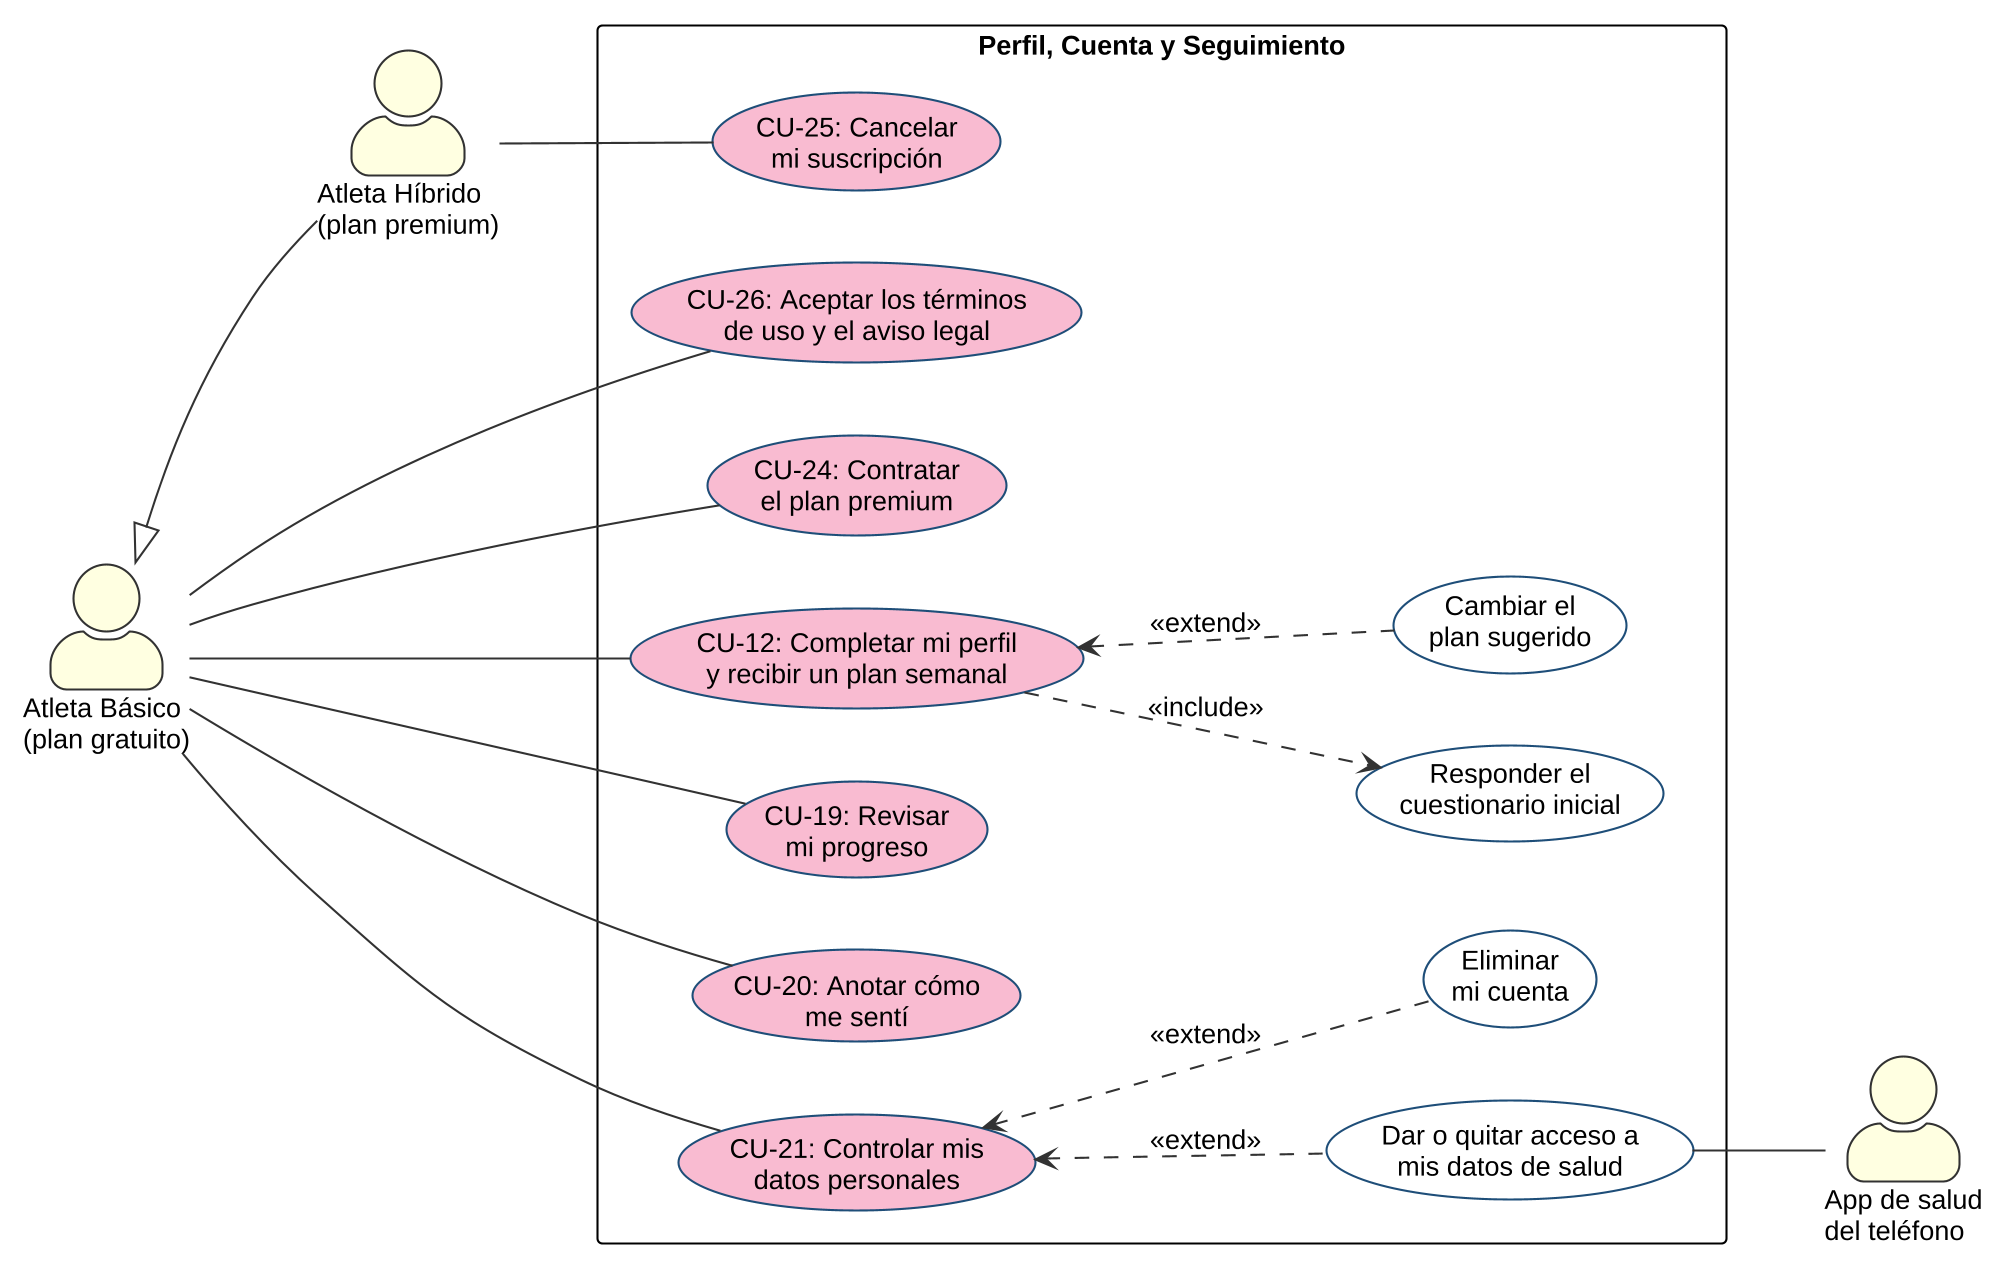
\includegraphics[width=0.9\textwidth]{figuras/casos_de_uso/cu_perfil.png}
    \caption{Diagrama de Casos de Uso: Perfil, Cuenta y Seguimiento.}
    \label{fig:cu_perfil}
\end{figure}

\begin{figure}[h!]
    \centering
    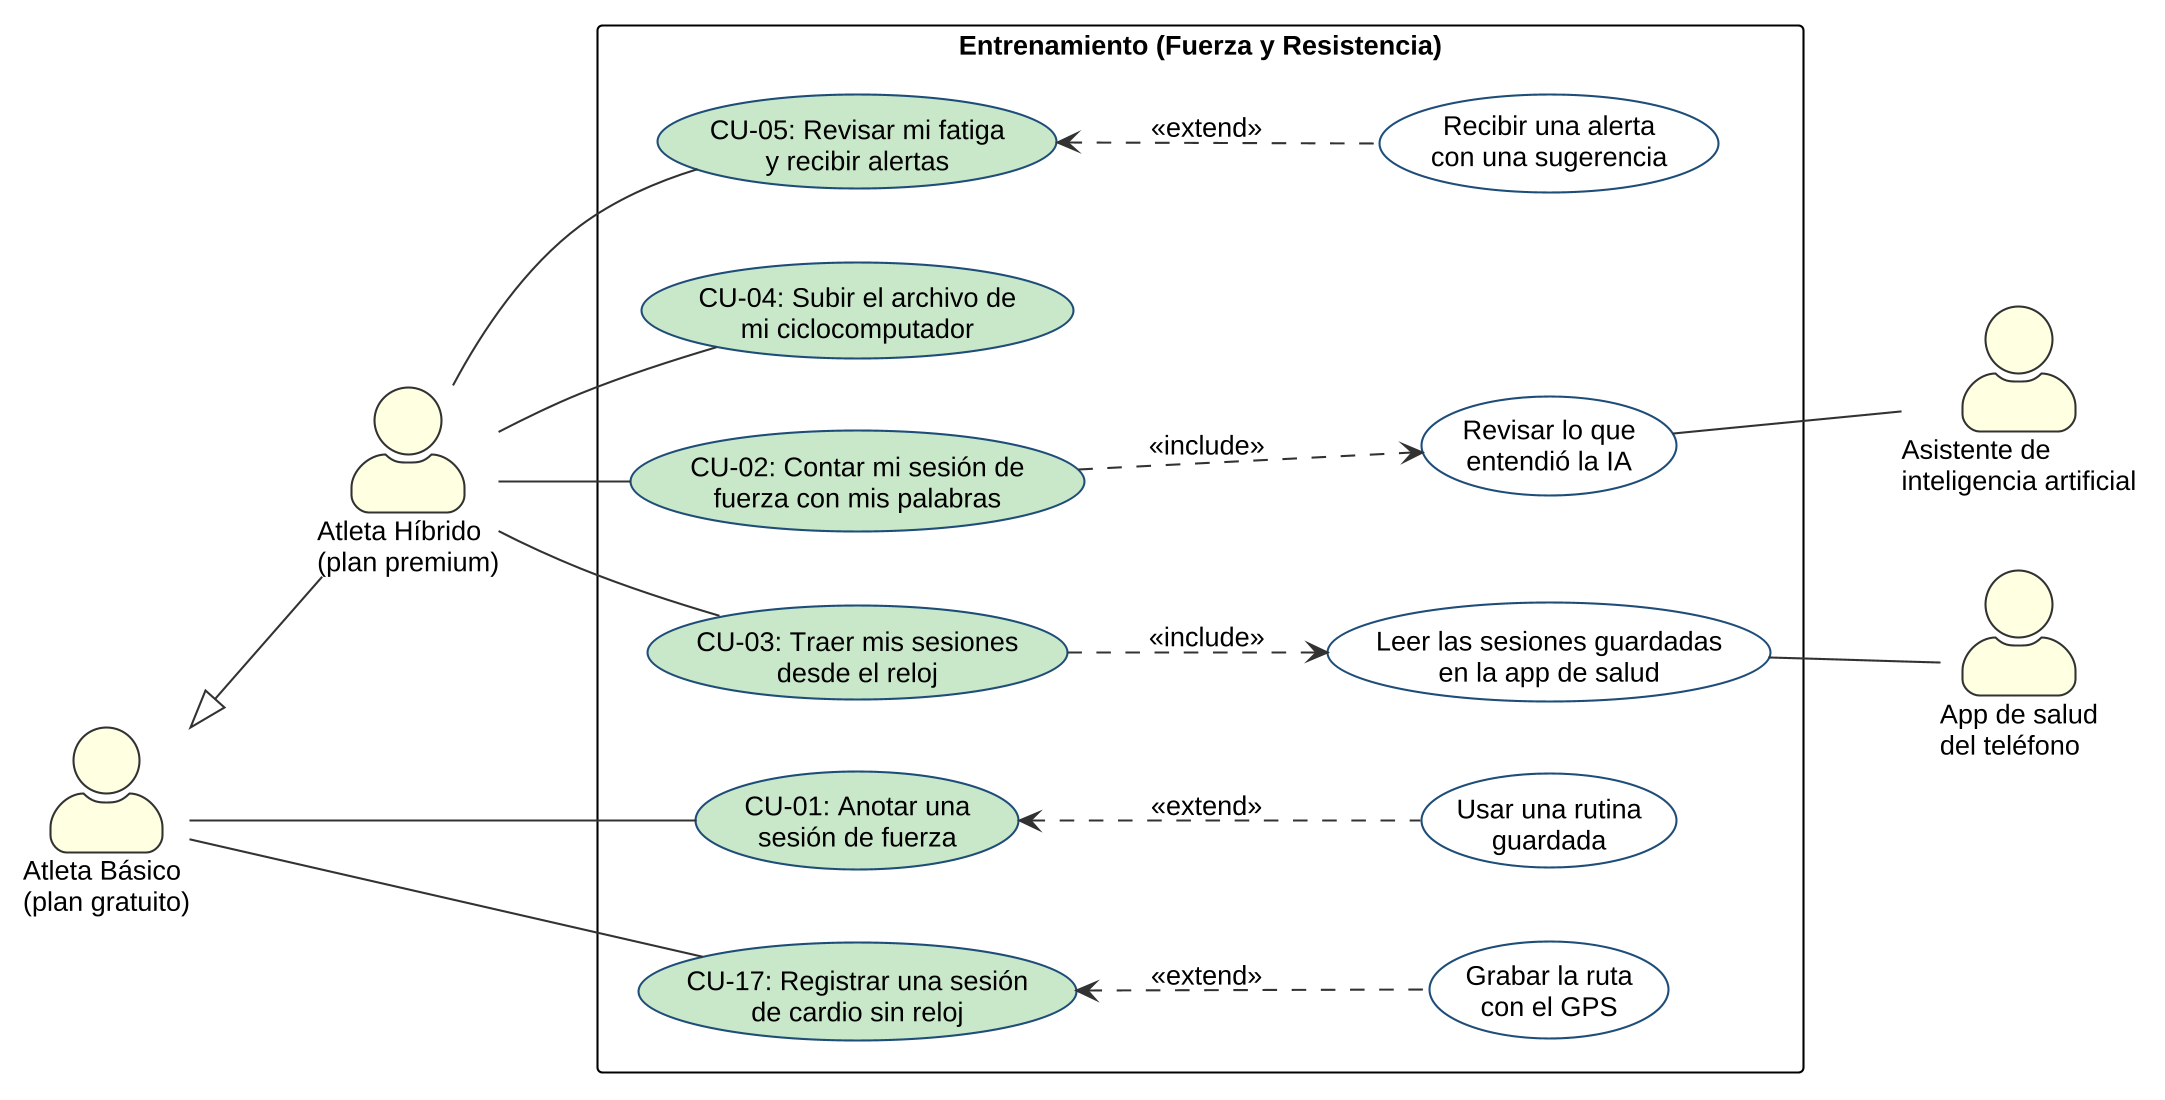
\includegraphics[width=0.95\textwidth]{figuras/casos_de_uso/cu_entrenamiento.png}
    \caption{Diagrama de Casos de Uso: Entrenamiento (Fuerza y Resistencia).}
    \label{fig:cu_entrenamiento}
\end{figure}
\begin{figure}[h!]
    \centering
    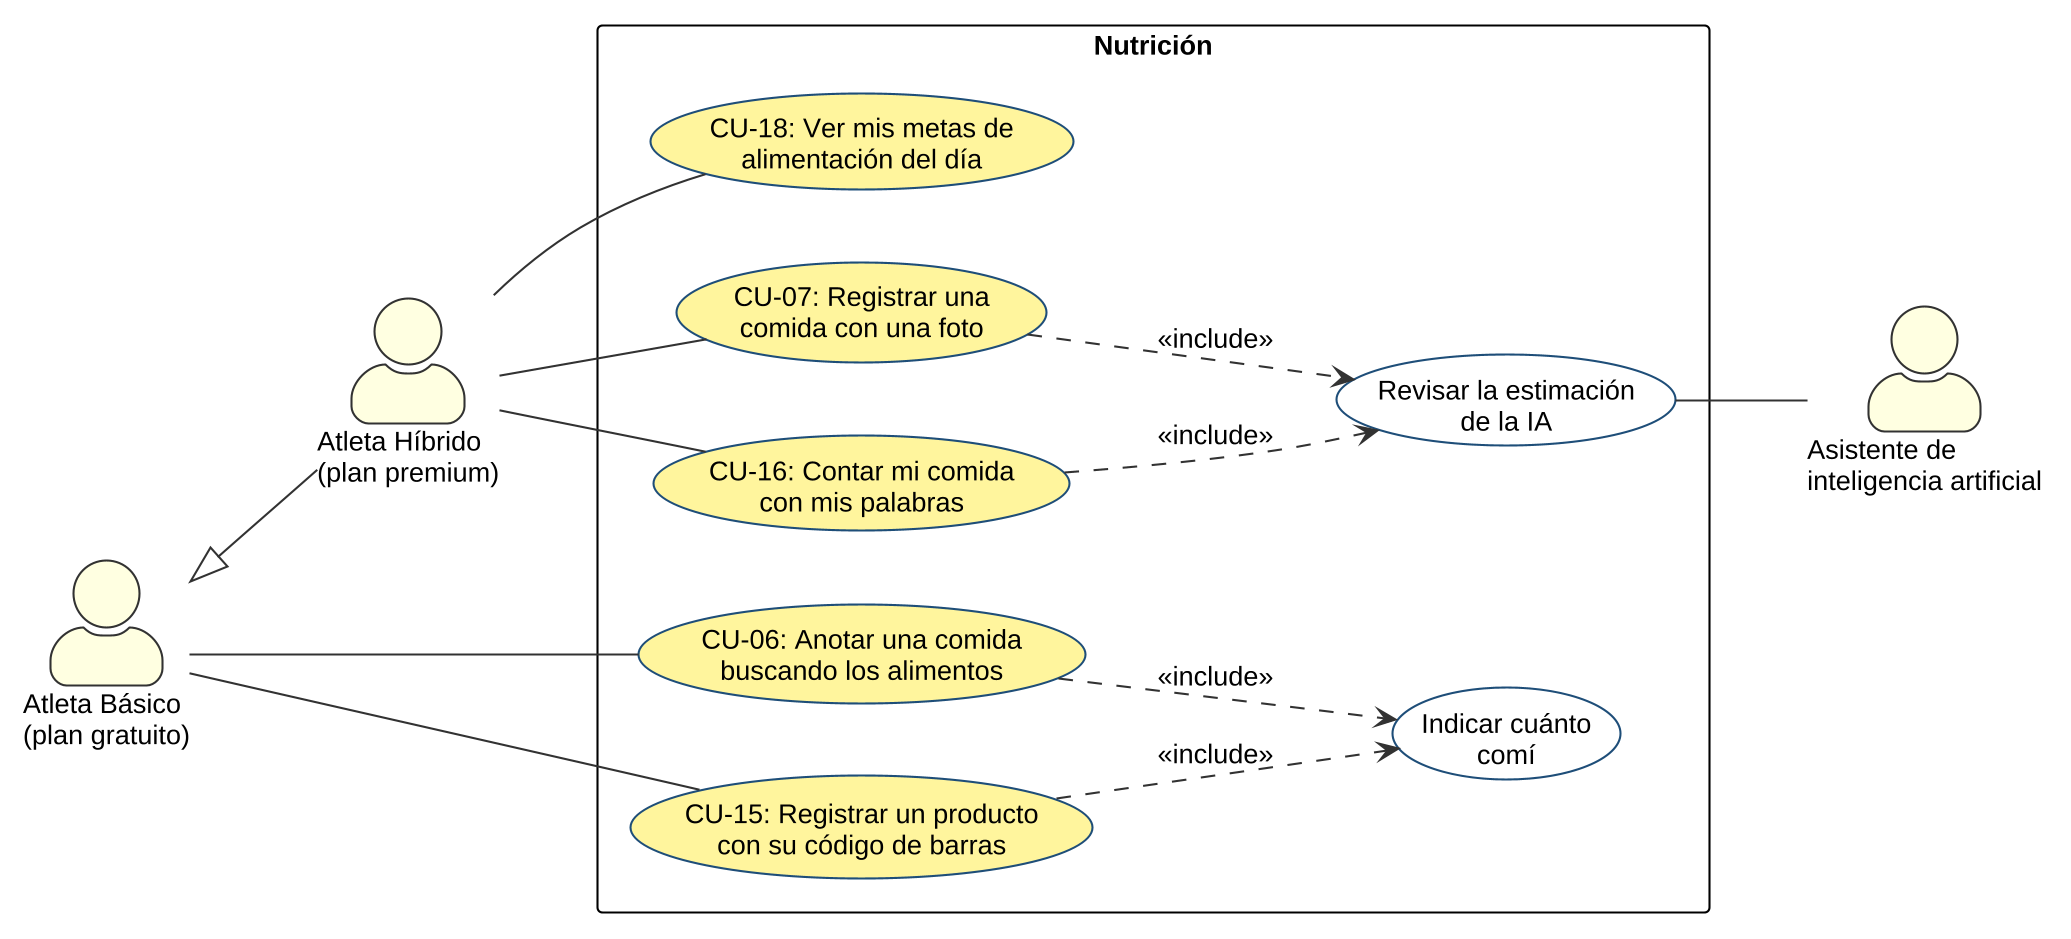
\includegraphics[width=0.95\textwidth]{figuras/casos_de_uso/cu_nutricion.png}
    \caption{Diagrama de Casos de Uso: Nutrición.}
    \label{fig:cu_nutricion}
\end{figure}

\begin{figure}[h!]
    \centering
    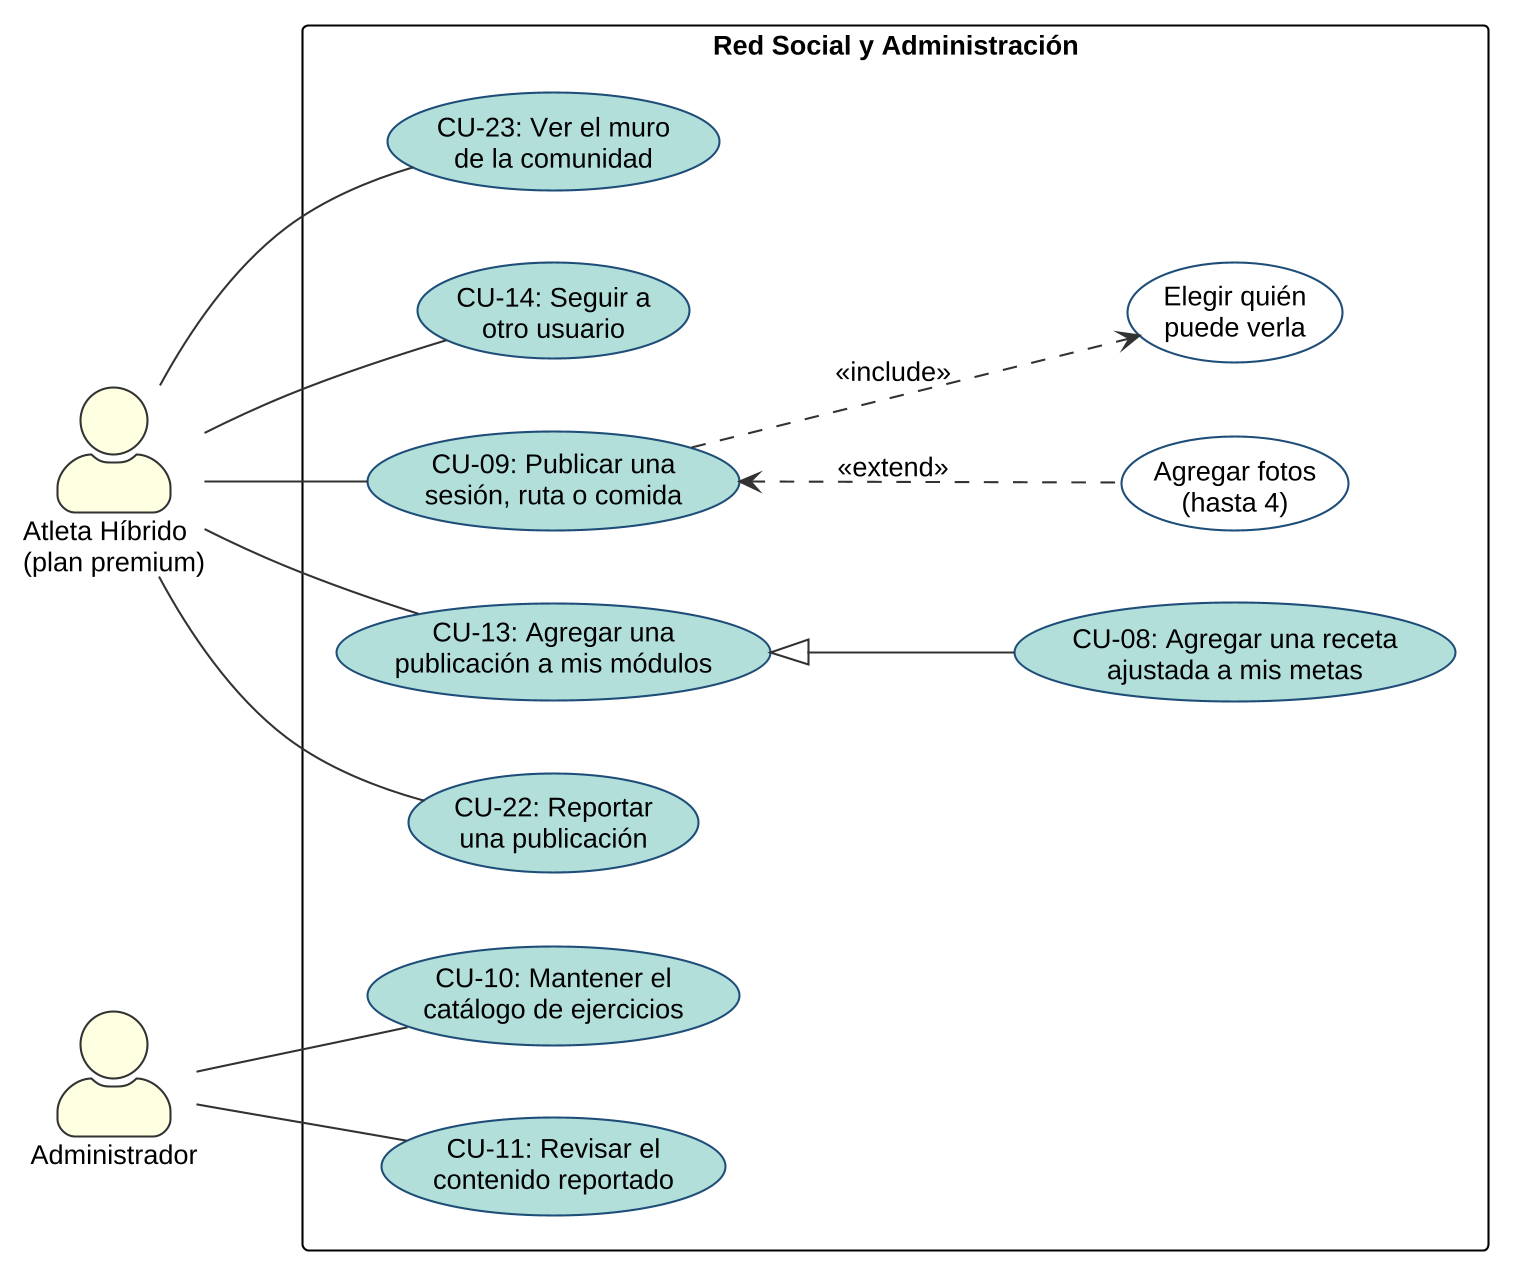
\includegraphics[width=0.85\textwidth]{figuras/casos_de_uso/cu_comunidad.png}
    \caption{Diagrama de Casos de Uso: Red Social y Administración.}
    \label{fig:cu_comunidad}
\end{figure}
\clearpage
\subsubsection{Descripción de Alto Nivel de Casos de Uso}
A continuación se describe cada caso de uso de los diagramas anteriores, con el requerimiento funcional al que responde. Su flujo normal y sus flujos alternativos se detallan en el Diseño Funcional del capítulo siguiente. Los casos CU-01 a CU-14 vienen de las versiones anteriores del documento, y los casos CU-15 a CU-26 se agregaron para que todos los requerimientos tengan al menos un caso de uso.

\noindent
\begin{tabular}{|p{3.5cm}|p{11.5cm}|}
    \hline
    \rowcolor[HTML]{EFEFEF}
    \textbf{Identificador} & \textbf{CU-01} \\ \hline
    \textbf{Nombre} & Anotar una sesión de fuerza \\ \hline
    \textbf{Actor Principal} & Atleta Básico / Atleta Híbrido \\ \hline
    \textbf{Descripción} & El usuario elige los ejercicios que hizo, desde la lista de ejercicios o desde una rutina que guardó antes, y anota las series, las repeticiones, el peso y qué tan duro lo sintió. La aplicación guarda la sesión y la suma a su historial. \\ \hline
    \textbf{RF Asociados} & R01 \\ \hline
\end{tabular}
\vspace{0.5cm}

\noindent
\begin{tabular}{|p{3.5cm}|p{11.5cm}|}
    \hline
    \rowcolor[HTML]{EFEFEF}
    \textbf{Identificador} & \textbf{CU-02} \\ \hline
    \textbf{Nombre} & Contar mi sesión de fuerza con mis palabras \\ \hline
    \textbf{Actor Principal} & Atleta Híbrido \\ \hline
    \textbf{Actores Secundarios} & Asistente de inteligencia artificial \\ \hline
    \textbf{Descripción} & El usuario escribe o dicta lo que hizo, por ejemplo ``sentadilla, 4 series de 8 con 80 kilos''. La aplicación lo ordena en ejercicios, series y pesos, y se lo muestra para que lo revise. El usuario corrige lo que haga falta y lo guarda. \\ \hline
    \textbf{RF Asociados} & R01 \\ \hline
\end{tabular}
\vspace{0.5cm}
\newpage
\noindent
\begin{tabular}{|p{3.5cm}|p{11.5cm}|}
    \hline
    \rowcolor[HTML]{EFEFEF}
    \textbf{Identificador} & \textbf{CU-03} \\ \hline
    \textbf{Nombre} & Traer mis sesiones desde el reloj \\ \hline
    \textbf{Actor Principal} & Atleta Híbrido \\ \hline
    \textbf{Actores Secundarios} & App de salud del teléfono \\ \hline
    \textbf{Descripción} & Después de entrenar con su reloj, la aplicación trae sola las sesiones nuevas de ciclismo, running o trekking desde la app de salud del teléfono, con su duración, su distancia y su pulso. Así no tiene que anotar nada a mano. La primera vez, la aplicación le pide permiso para leer esos datos. \\ \hline
    \textbf{RF Asociados} & R02 \\ \hline
\end{tabular}
\vspace{0.5cm}

\noindent
\begin{tabular}{|p{3.5cm}|p{11.5cm}|}
    \hline
    \rowcolor[HTML]{EFEFEF}
    \textbf{Identificador} & \textbf{CU-04} \\ \hline
    \textbf{Nombre} & Subir el archivo de mi ciclocomputador \\ \hline
    \textbf{Actor Principal} & Atleta Híbrido \\ \hline
    \textbf{Descripción} & El usuario sube el archivo que exportó desde su ciclocomputador o reloj. La aplicación lo lee y le muestra la sesión con todo detalle, como la potencia, la cadencia y el pulso a lo largo de la salida. \\ \hline
    \textbf{RF Asociados} & R02 \\ \hline
\end{tabular}
\vspace{0.5cm}

\noindent
\begin{tabular}{|p{3.5cm}|p{11.5cm}|}
    \hline
    \rowcolor[HTML]{EFEFEF}
    \textbf{Identificador} & \textbf{CU-05} \\ \hline
    \textbf{Nombre} & Revisar mi fatiga y recibir alertas \\ \hline
    \textbf{Actor Principal} & Atleta Híbrido \\ \hline
    \textbf{Descripción} & El usuario ve en un resumen cuánto se ha cargado en la semana, sumando la fuerza y el cardio. Si la aplicación nota que viene muy cansado y tiene un entrenamiento exigente al día siguiente, le manda un aviso con una sugerencia, por ejemplo bajar el peso o mover la sesión. También le avisa si dejó poco tiempo entre una sesión de fuerza y una de cardio. El usuario decide si la sigue. \\ \hline
    \textbf{RF Asociados} & R03 \\ \hline
\end{tabular}
\vspace{0.5cm}
\newpage
\noindent
\begin{tabular}{|p{3.5cm}|p{11.5cm}|}
    \hline
    \rowcolor[HTML]{EFEFEF}
    \textbf{Identificador} & \textbf{CU-06} \\ \hline
    \textbf{Nombre} & Anotar una comida buscando los alimentos \\ \hline
    \textbf{Actor Principal} & Atleta Básico / Atleta Híbrido \\ \hline
    \textbf{Descripción} & El usuario busca lo que comió en la lista de alimentos, indica cuánto comió y lo guarda en su diario del día. La aplicación le muestra las calorías y los macronutrientes de la comida y cuánto lleva en el día. \\ \hline
    \textbf{RF Asociados} & R04 \\ \hline
\end{tabular}
\vspace{0.5cm}

\noindent
\begin{tabular}{|p{3.5cm}|p{11.5cm}|}
    \hline
    \rowcolor[HTML]{EFEFEF}
    \textbf{Identificador} & \textbf{CU-07} \\ \hline
    \textbf{Nombre} & Registrar una comida con una foto \\ \hline
    \textbf{Actor Principal} & Atleta Híbrido \\ \hline
    \textbf{Actores Secundarios} & Asistente de inteligencia artificial \\ \hline
    \textbf{Descripción} & El usuario le saca una foto a su plato. La aplicación estima qué alimentos hay, en qué cantidad y cuántas calorías y macronutrientes tienen. El usuario revisa la estimación, la corrige si hace falta y la guarda. Cuando la aplicación no está segura del resultado, se lo avisa para que lo revise con más cuidado. La foto no se guarda, salvo que el usuario la quiera publicar. \\ \hline
    \textbf{RF Asociados} & R04 \\ \hline
\end{tabular}
\vspace{0.5cm}

\noindent
\begin{tabular}{|p{3.5cm}|p{11.5cm}|}
    \hline
    \rowcolor[HTML]{EFEFEF}
    \textbf{Identificador} & \textbf{CU-08} \\ \hline
    \textbf{Nombre} & Agregar una receta ajustada a mis metas \\ \hline
    \textbf{Actor Principal} & Atleta Híbrido \\ \hline
    \textbf{Descripción} & El usuario ve una receta en el muro y la agrega a su módulo de nutrición. La aplicación ajusta la cantidad de cada ingrediente según lo que le falta comer ese día, manteniendo las proporciones de la receta original. Es un caso particular de CU-13. \\ \hline
    \textbf{RF Asociados} & R12 \\ \hline
\end{tabular}
\vspace{0.5cm}
\newpage
\noindent
\begin{tabular}{|p{3.5cm}|p{11.5cm}|}
    \hline
    \rowcolor[HTML]{EFEFEF}
    \textbf{Identificador} & \textbf{CU-09} \\ \hline
    \textbf{Nombre} & Publicar una sesión, ruta o comida \\ \hline
    \textbf{Actor Principal} & Atleta Híbrido \\ \hline
    \textbf{Descripción} & El usuario elige una sesión de fuerza, una ruta o una comida que ya registró, le agrega un texto y, si quiere, hasta 4 fotos, declarando que son suyas o que tiene permiso para publicarlas. Luego elige quién la puede ver (todos, sus seguidores o solo él). Si publica una ruta, la aplicación oculta el inicio y el final del recorrido para que no se sepa dónde vive. \\ \hline
    \textbf{RF Asociados} & R08 \\ \hline
\end{tabular}
\vspace{0.5cm}

\noindent
\begin{tabular}{|p{3.5cm}|p{11.5cm}|}
    \hline
    \rowcolor[HTML]{EFEFEF}
    \textbf{Identificador} & \textbf{CU-10} \\ \hline
    \textbf{Nombre} & Mantener el catálogo de ejercicios \\ \hline
    \textbf{Actor Principal} & Administrador \\ \hline
    \textbf{Descripción} & El administrador agrega, cambia o desactiva ejercicios de la lista que usan los atletas, indicando qué músculos trabajan y qué equipamiento necesitan. La aplicación le avisa si el ejercicio ya existe. \\ \hline
    \textbf{RF Asociados} & R11 \\ \hline
\end{tabular}
\vspace{0.5cm}

\noindent
\begin{tabular}{|p{3.5cm}|p{11.5cm}|}
    \hline
    \rowcolor[HTML]{EFEFEF}
    \textbf{Identificador} & \textbf{CU-11} \\ \hline
    \textbf{Nombre} & Revisar el contenido reportado \\ \hline
    \textbf{Actor Principal} & Administrador \\ \hline
    \textbf{Descripción} & El administrador revisa las publicaciones, fotos y recetas que reportaron los usuarios. Si no cumplen las normas de la comunidad o pueden ser peligrosas para la salud, las oculta. La aplicación guarda quién tomó la decisión y por qué. \\ \hline
    \textbf{RF Asociados} & R11 \\ \hline
\end{tabular}
\vspace{0.5cm}
\newpage
\noindent
\begin{tabular}{|p{3.5cm}|p{11.5cm}|}
    \hline
    \rowcolor[HTML]{EFEFEF}
    \textbf{Identificador} & \textbf{CU-12} \\ \hline
    \textbf{Nombre} & Completar mi perfil y recibir un plan semanal \\ \hline
    \textbf{Actor Principal} & Atleta Básico / Atleta Híbrido \\ \hline
    \textbf{Descripción} & Al crear su cuenta, el usuario responde preguntas sobre su experiencia, sus objetivos, los días que puede entrenar, su equipamiento, los deportes que practica, su edad, su sexo, su estatura y su peso. Con eso, la aplicación le sugiere un plan para la semana, que puede aceptar, cambiar o ignorar. Cada semana el plan se ajusta según lo que el usuario cumplió y cómo se sintió. \\ \hline
    \textbf{RF Asociados} & R13 \\ \hline
\end{tabular}
\vspace{0.5cm}

\noindent
\begin{tabular}{|p{3.5cm}|p{11.5cm}|}
    \hline
    \rowcolor[HTML]{EFEFEF}
    \textbf{Identificador} & \textbf{CU-13} \\ \hline
    \textbf{Nombre} & Agregar una publicación a mis módulos \\ \hline
    \textbf{Actor Principal} & Atleta Híbrido \\ \hline
    \textbf{Descripción} & El usuario ve en el muro una publicación de otra persona, por ejemplo una rutina de pecho, y pulsa ``Agregar a mis rutinas''. La rutina queda guardada como suya, indicando quién la creó. Si es una ruta, queda en su módulo de cardio, y si es una receta, en su módulo de nutrición (CU-08). \\ \hline
    \textbf{RF Asociados} & R12 \\ \hline
\end{tabular}
\vspace{0.5cm}

\noindent
\begin{tabular}{|p{3.5cm}|p{11.5cm}|}
    \hline
    \rowcolor[HTML]{EFEFEF}
    \textbf{Identificador} & \textbf{CU-14} \\ \hline
    \textbf{Nombre} & Seguir a otro usuario \\ \hline
    \textbf{Actor Principal} & Atleta Híbrido \\ \hline
    \textbf{Descripción} & El usuario encuentra a otra persona en el muro o en el buscador y la sigue. Desde ese momento ve las publicaciones de esa persona en su muro. Puede dejar de seguirla cuando quiera. \\ \hline
    \textbf{RF Asociados} & R08 \\ \hline
\end{tabular}
\vspace{0.5cm}
\newpage
\noindent
\begin{tabular}{|p{3.5cm}|p{11.5cm}|}
    \hline
    \rowcolor[HTML]{EFEFEF}
    \textbf{Identificador} & \textbf{CU-15} \\ \hline
    \textbf{Nombre} & Registrar un producto con su código de barras \\ \hline
    \textbf{Actor Principal} & Atleta Básico / Atleta Híbrido \\ \hline
    \textbf{Descripción} & El usuario escanea con la cámara el código de barras de un producto envasado. La aplicación le muestra sus calorías y macronutrientes. El usuario indica cuánto comió y lo guarda. \\ \hline
    \textbf{RF Asociados} & R04 \\ \hline
\end{tabular}
\vspace{0.5cm}

\noindent
\begin{tabular}{|p{3.5cm}|p{11.5cm}|}
    \hline
    \rowcolor[HTML]{EFEFEF}
    \textbf{Identificador} & \textbf{CU-16} \\ \hline
    \textbf{Nombre} & Contar mi comida con mis palabras \\ \hline
    \textbf{Actor Principal} & Atleta Híbrido \\ \hline
    \textbf{Actores Secundarios} & Asistente de inteligencia artificial \\ \hline
    \textbf{Descripción} & El usuario escribe o dicta lo que comió, por ejemplo ``un plato de arroz con pollo y una ensalada''. La aplicación estima los alimentos, las cantidades y los macronutrientes. El usuario revisa la estimación, la corrige si hace falta y la guarda. \\ \hline
    \textbf{RF Asociados} & R04 \\ \hline
\end{tabular}
\vspace{0.5cm}

\noindent
\begin{tabular}{|p{3.5cm}|p{11.5cm}|}
    \hline
    \rowcolor[HTML]{EFEFEF}
    \textbf{Identificador} & \textbf{CU-17} \\ \hline
    \textbf{Nombre} & Registrar una sesión de cardio sin reloj \\ \hline
    \textbf{Actor Principal} & Atleta Básico / Atleta Híbrido \\ \hline
    \textbf{Descripción} & El usuario graba su salida de ciclismo, running o trekking con el GPS del teléfono, o la anota a mano con su duración, su distancia y qué tan duro la sintió. La aplicación la guarda y la considera en su carga de la semana. \\ \hline
    \textbf{RF Asociados} & R02 \\ \hline
\end{tabular}
\vspace{0.5cm}
\newpage
\noindent
\begin{tabular}{|p{3.5cm}|p{11.5cm}|}
    \hline
    \rowcolor[HTML]{EFEFEF}
    \textbf{Identificador} & \textbf{CU-18} \\ \hline
    \textbf{Nombre} & Ver mis metas de alimentación del día \\ \hline
    \textbf{Actor Principal} & Atleta Híbrido \\ \hline
    \textbf{Descripción} & El usuario abre su resumen de nutrición y ve cuántas calorías y macronutrientes le conviene comer ese día, según lo que entrenó o tiene planificado, y cuánto le falta. También le sugiere en qué momento conviene comer. Son sugerencias y no una dieta. \\ \hline
    \textbf{RF Asociados} & R05 \\ \hline
\end{tabular}
\vspace{0.5cm}

\noindent
\begin{tabular}{|p{3.5cm}|p{11.5cm}|}
    \hline
    \rowcolor[HTML]{EFEFEF}
    \textbf{Identificador} & \textbf{CU-19} \\ \hline
    \textbf{Nombre} & Revisar mi progreso \\ \hline
    \textbf{Actor Principal} & Atleta Básico / Atleta Híbrido \\ \hline
    \textbf{Descripción} & El usuario abre su historial y elige ver un día o un mes. La aplicación le muestra juntos sus entrenamientos, sus comidas y cómo ha cambiado su carga en el tiempo. \\ \hline
    \textbf{RF Asociados} & R06 \\ \hline
\end{tabular}
\vspace{0.5cm}

\noindent
\begin{tabular}{|p{3.5cm}|p{11.5cm}|}
    \hline
    \rowcolor[HTML]{EFEFEF}
    \textbf{Identificador} & \textbf{CU-20} \\ \hline
    \textbf{Nombre} & Anotar cómo me sentí \\ \hline
    \textbf{Actor Principal} & Atleta Básico / Atleta Híbrido \\ \hline
    \textbf{Descripción} & Después de un entrenamiento o de una comida, el usuario escribe cómo se sintió, por ejemplo si tuvo alguna molestia o si la comida le cayó pesada. La nota queda junto a ese registro para revisarla después. \\ \hline
    \textbf{RF Asociados} & R07 \\ \hline
\end{tabular}
\vspace{0.5cm}
\newpage
\noindent
\begin{tabular}{|p{3.5cm}|p{11.5cm}|}
    \hline
    \rowcolor[HTML]{EFEFEF}
    \textbf{Identificador} & \textbf{CU-21} \\ \hline
    \textbf{Nombre} & Controlar mis datos personales \\ \hline
    \textbf{Actor Principal} & Atleta Básico / Atleta Híbrido \\ \hline
    \textbf{Actores Secundarios} & App de salud del teléfono \\ \hline
    \textbf{Descripción} & El usuario decide si la aplicación puede leer sus datos de salud y puede cambiar esa decisión cuando quiera. También puede revisar y corregir sus datos o eliminar su cuenta. Si elimina la cuenta, se borran todos sus datos. \\ \hline
    \textbf{RF Asociados} & R09 \\ \hline
\end{tabular}
\vspace{0.5cm}

\noindent
\begin{tabular}{|p{3.5cm}|p{11.5cm}|}
    \hline
    \rowcolor[HTML]{EFEFEF}
    \textbf{Identificador} & \textbf{CU-22} \\ \hline
    \textbf{Nombre} & Reportar una publicación \\ \hline
    \textbf{Actor Principal} & Atleta Híbrido \\ \hline
    \textbf{Descripción} & El usuario reporta una publicación o una foto que le parece inapropiada o peligrosa y elige el motivo. El administrador la revisa después (CU-11). \\ \hline
    \textbf{RF Asociados} & R08, R11 \\ \hline
\end{tabular}
\vspace{0.5cm}

\noindent
\begin{tabular}{|p{3.5cm}|p{11.5cm}|}
    \hline
    \rowcolor[HTML]{EFEFEF}
    \textbf{Identificador} & \textbf{CU-23} \\ \hline
    \textbf{Nombre} & Ver el muro de la comunidad \\ \hline
    \textbf{Actor Principal} & Atleta Híbrido \\ \hline
    \textbf{Descripción} & El usuario abre el muro y ve las publicaciones más recientes de las personas que sigue, con sus fotos. Desde ahí puede abrir una publicación, agregarla a sus módulos (CU-13) o reportarla (CU-22). \\ \hline
    \textbf{RF Asociados} & R08 \\ \hline
\end{tabular}
\vspace{0.5cm}

\noindent
\begin{tabular}{|p{3.5cm}|p{11.5cm}|}
    \hline
    \rowcolor[HTML]{EFEFEF}
    \textbf{Identificador} & \textbf{CU-24} \\ \hline
    \textbf{Nombre} & Contratar el plan premium \\ \hline
    \textbf{Actor Principal} & Atleta Básico \\ \hline
    \textbf{Descripción} & El usuario ve qué incluye el plan premium, cuánto cuesta en total y cada cuánto se cobra. Si le interesa, lo contrata y desde ese momento tiene todas sus funciones. \\ \hline
    \textbf{RF Asociados} & R14 \\ \hline
\end{tabular}
\vspace{0.5cm}

\noindent
\begin{tabular}{|p{3.5cm}|p{11.5cm}|}
    \hline
    \rowcolor[HTML]{EFEFEF}
    \textbf{Identificador} & \textbf{CU-25} \\ \hline
    \textbf{Nombre} & Cancelar mi suscripción \\ \hline
    \textbf{Actor Principal} & Atleta Híbrido \\ \hline
    \textbf{Descripción} & El usuario cancela su suscripción desde la aplicación, que lo lleva a la pantalla de suscripciones de su tienda, donde confirma la cancelación. Sigue con el plan premium hasta que termine el periodo pagado, y después vuelve al plan gratuito conservando sus datos. \\ \hline
    \textbf{RF Asociados} & R14 \\ \hline
\end{tabular}
\vspace{0.5cm}

\noindent
\begin{tabular}{|p{3.5cm}|p{11.5cm}|}
    \hline
    \rowcolor[HTML]{EFEFEF}
    \textbf{Identificador} & \textbf{CU-26} \\ \hline
    \textbf{Nombre} & Aceptar los términos de uso y el aviso legal \\ \hline
    \textbf{Actor Principal} & Atleta Básico / Atleta Híbrido \\ \hline
    \textbf{Descripción} & Al crear su cuenta, el usuario lee los términos de uso y el aviso legal, y los acepta para poder seguir. Si los términos cambian más adelante, la aplicación se los vuelve a mostrar. \\ \hline
    \textbf{RF Asociados} & R15 \\ \hline
\end{tabular}
\vspace{0.5cm}
\newpage
\begin{table}[h!]
    \centering
    \renewcommand{\arraystretch}{1.3}
    \begin{tabular}{|p{1.5cm}|>{\raggedright\arraybackslash}p{7cm}|>{\raggedright\arraybackslash}p{6cm}|}
        \hline
        \rowcolor[HTML]{EFEFEF}
        \textbf{ID} & \textbf{Requerimiento} & \textbf{Casos de uso} \\ \hline
        R01 & Registro de entrenamientos de fuerza & CU-01, CU-02 \\ \hline
        R02 & Registro de entrenamientos de resistencia & CU-03, CU-04, CU-17 \\ \hline
        R03 & Alertas de fatiga y ajuste del entrenamiento & CU-05 \\ \hline
        R04 & Registro de comidas & CU-06, CU-07, CU-15, CU-16 \\ \hline
        R05 & Metas de alimentación según el entrenamiento & CU-18 \\ \hline
        R06 & Seguimiento del progreso & CU-19 \\ \hline
        R07 & Registro de sensaciones & CU-20 \\ \hline
        R08 & Red social deportiva & CU-09, CU-14, CU-22, CU-23 \\ \hline
        R09 & Control de datos personales & CU-21 \\ \hline
        R10 & Uso simple y rápido & Se cubre en todos los casos de uso y con los requisitos no funcionales. \\ \hline
        R11 & Administración de la plataforma & CU-10, CU-11, CU-22 \\ \hline
        R12 & Agregar contenido de la comunidad a mis módulos & CU-08, CU-13 \\ \hline
        R13 & Perfil del usuario y plan sugerido & CU-12 \\ \hline
        R14 & Suscripción al plan premium & CU-24, CU-25 \\ \hline
        R15 & Términos de uso y aviso legal & CU-09, CU-26 \\ \hline
    \end{tabular}
    \caption{Relación entre los requerimientos funcionales y los casos de uso.}
    \label{tab:cu_requerimientos}
\end{table}
\newpage
\subsection{Comentarios Generales del Capítulo}
En este capítulo se ha consolidado el puente entre la visión de negocio y la implementación técnica de la plataforma. El capítulo partió con un Modelo de Negocios de cinco procesos, que son el registro de cardio con el cálculo de fatiga, el registro de comidas con sus metas, la publicación y el uso de contenido de la comunidad, el registro de fuerza y el plan sugerido. Posteriormente, la trazabilidad de los requerimientos garantizó que cada especificación funcional y no funcional del software nazca directamente de una necesidad operativa comprobada, mitigando el riesgo de desarrollar funcionalidades superfluas. 

Además, se incorporaron requerimientos centrados en la personalización, como el perfil del usuario con su plan sugerido, y en la red social deportiva, donde el contenido que publican otros usuarios se puede agregar directamente a los propios módulos.
\\\\
Finalmente, la especificación de los Casos de Uso, apoyada por sus respectivos diagramas e identificación de actores primarios y secundarios, delimitó con exactitud la frontera del sistema. Con este sólido marco de requerimientos finalizado, alineado a las restricciones normativas chilenas y a las dependencias de hardware de terceros, el proyecto cuenta con las bases necesarias para transicionar hacia la fase de Ingeniería de Diseño, donde se definirá la arquitectura de software detallada, el modelo de datos orientado a documentos y las interfaces de usuario.\newpage
\newpage

% Ingeniería de Diseño
% Este archivo se incluye desde main.tex con \input.
\section{Ingeniería de Diseño}
\subsection{Introducción del Capítulo}
El presente capítulo detalla la Ingeniería de Diseño de la solución tecnológica. Tomando como base los requerimientos funcionales y las restricciones operativas definidas en el capítulo anterior, aquí se materializa la arquitectura del software, la estructuración de la base de datos, el diseño de las interfaces de usuario y el modelo de interacciones. El objetivo de este diseño es garantizar que la plataforma sea escalable, segura y capaz de procesar la telemetría concurrente y los modelos de inteligencia artificial de forma eficiente.

\subsection{Diagrama de Sistema de Alto Nivel}
La Figura \ref{fig:arquitectura_alto_nivel} muestra las partes principales de la plataforma y cómo se comunican. El sistema sigue un modelo cliente-servidor con una API REST, y se divide en tres capas, que son la capa de presentación, la capa de procesamiento en la nube y la capa de servicios externos.

\begin{figure}[!htbp]
    \centering
    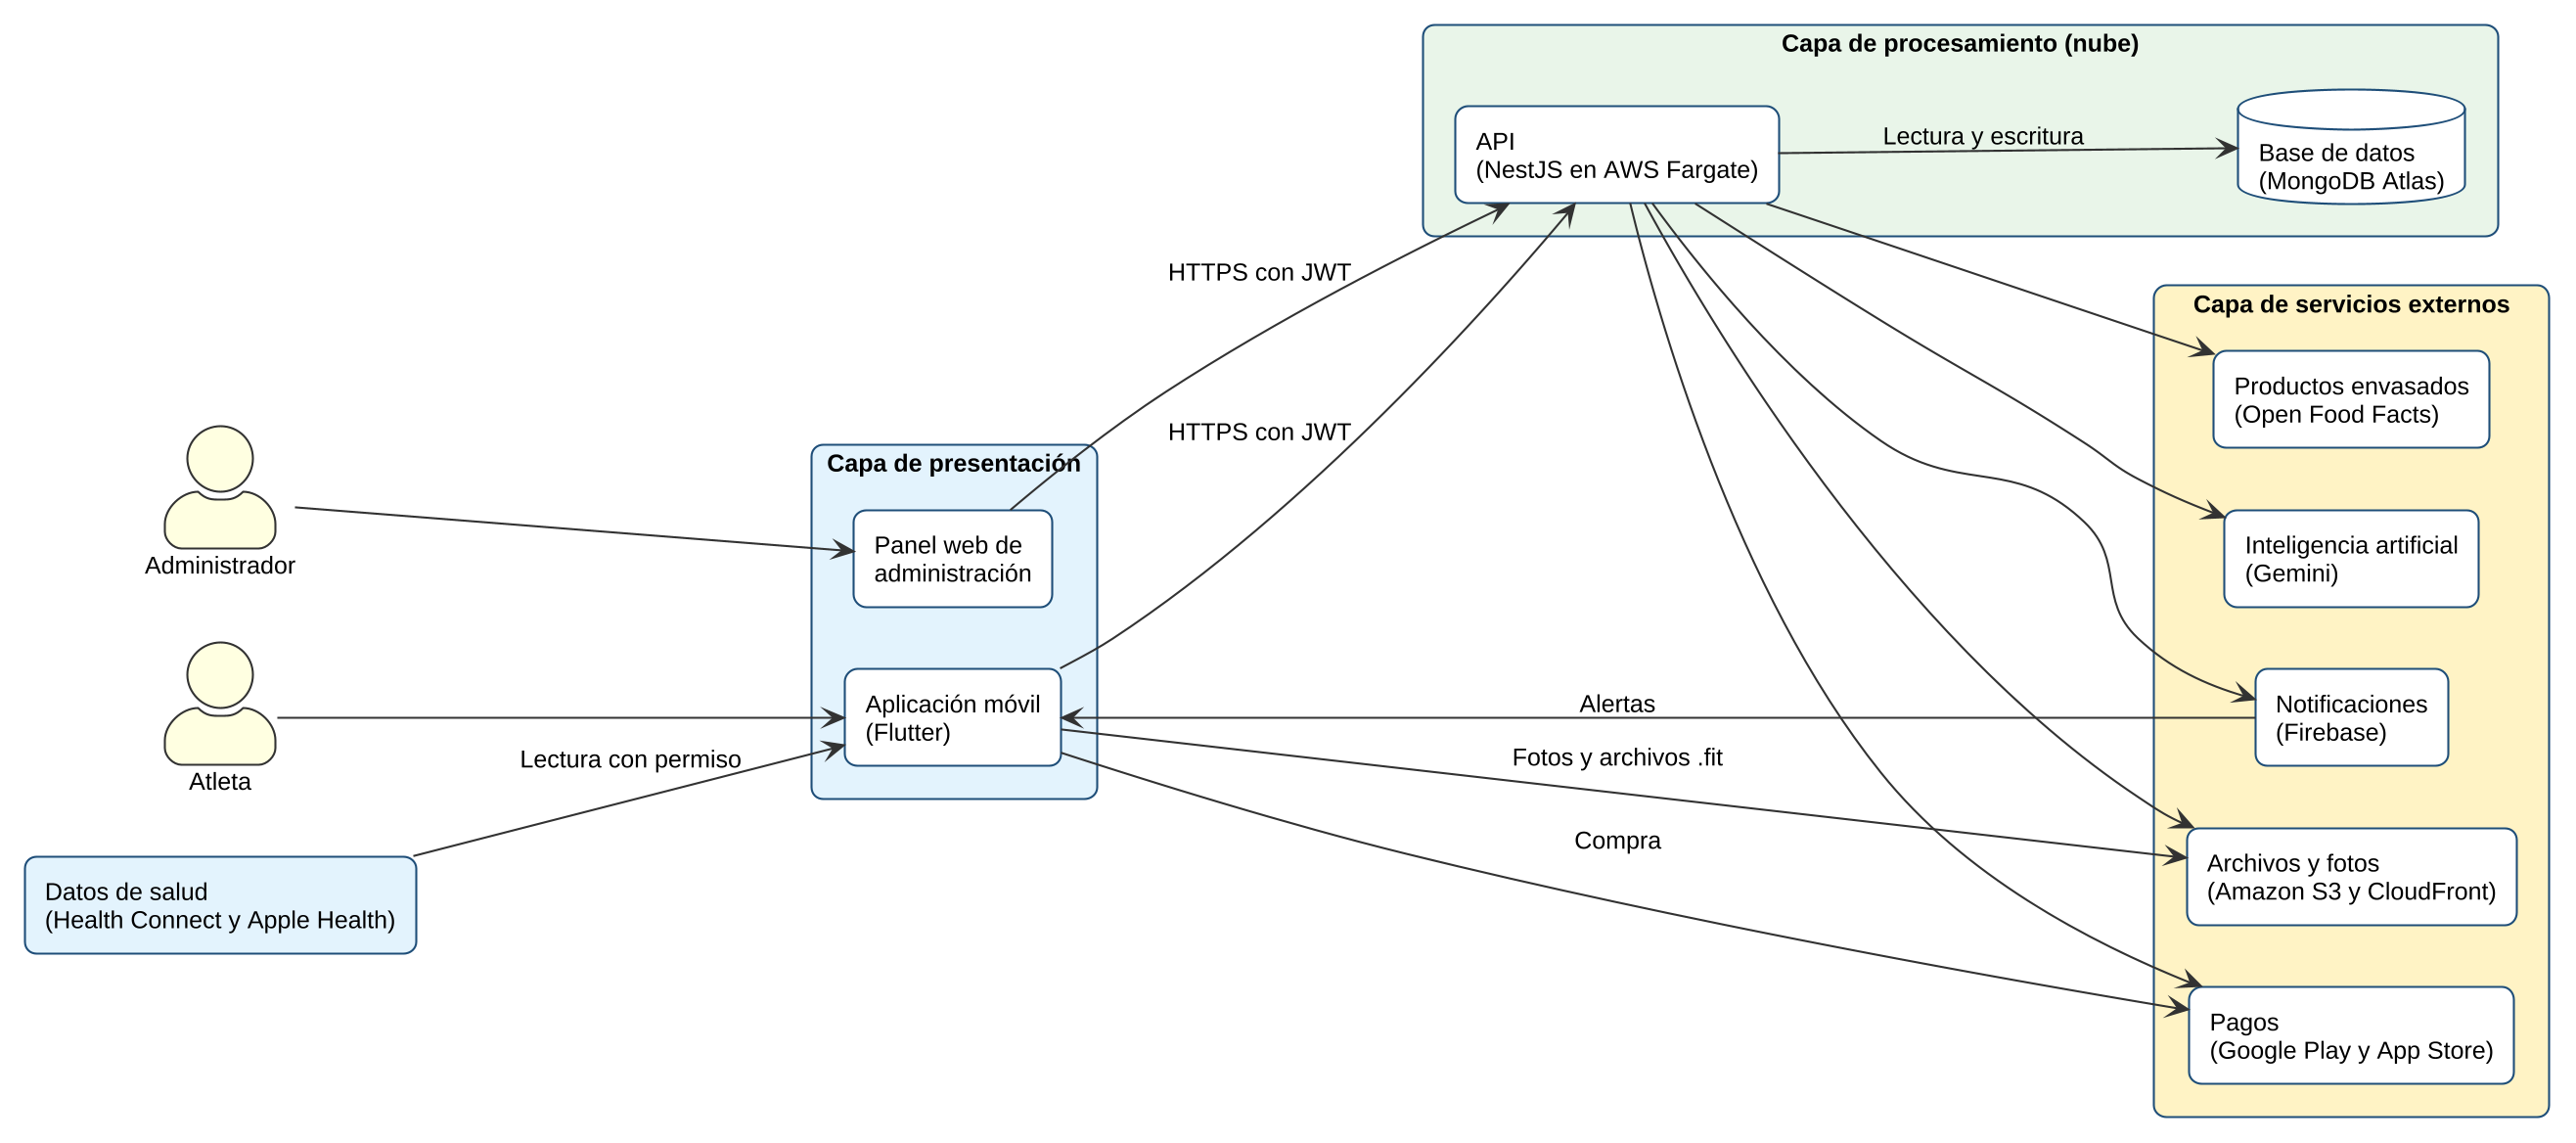
\includegraphics[width=1\textwidth]{figuras/arquitectura/diagrama_arquitectura.png}
    \caption{Arquitectura de Alto Nivel del Sistema.}
    \label{fig:arquitectura_alto_nivel}
\end{figure}
La \textbf{capa de presentación} es lo que usan las personas. El atleta usa la aplicación móvil hecha en \textbf{Flutter}, y el administrador usa un panel web. Además, la aplicación lee, con permiso del usuario, los datos de salud que Health Connect o Apple Health reúnen en el mismo teléfono.

La \textbf{capa de procesamiento} está en la nube. Una API hecha en \textbf{NestJS}, que corre en AWS Fargate, concentra la lógica del sistema, como el cálculo de la fatiga, las metas de alimentación y el plan sugerido. Es la única parte con acceso a la base de datos \textbf{MongoDB}, alojada en MongoDB Atlas, y revisa cada documento antes de guardarlo.

La \textbf{capa de servicios externos} reúne lo que el proyecto no construye por su cuenta. Gemini interpreta las fotos de comida y los textos, Open Food Facts entrega los datos de los productos envasados, Firebase envía las alertas al teléfono, Amazon S3 y CloudFront guardan y muestran los archivos y las fotos, y Google Play y App Store se encargan de los pagos. La mayoría de estas conexiones parte desde la API. Las excepciones son la subida de archivos, la visualización de fotos y el pago, que la aplicación hace directamente. El detalle de cada conexión se explica en la sección Diagrama de Integraciones.
\subsection{Diseño Funcional}
A continuación se presentan los flujos de cada uno de los casos de uso descritos en la fase de requerimientos. Para cada uno se indican sus precondiciones y poscondiciones, su curso normal de eventos y sus cursos alternos. Cada curso alterno lleva el número del paso del curso normal en el que ocurre.

\subsubsection{CU-01. Anotar una sesión de fuerza}

\textbf{Diagrama de Actividades}
\begin{center}
    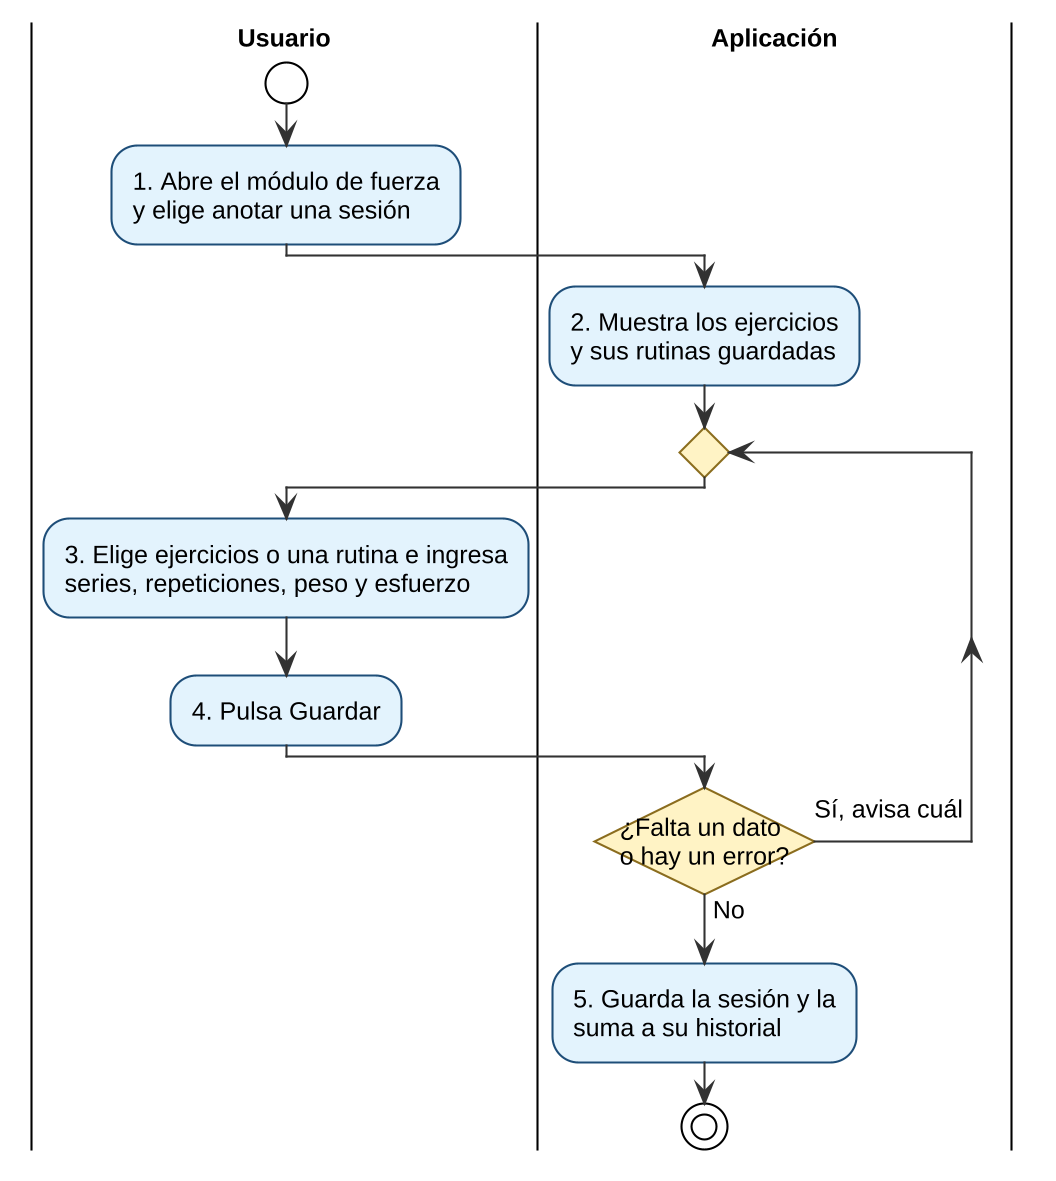
\includegraphics[width=0.78\textwidth,height=0.42\textheight,keepaspectratio]{figuras/diseno/dga_cu01.png}
    \captionof{figure}{Diagrama de Actividades -- CU-01: Anotar una sesión de fuerza.}
    \label{fig:dga_cu01}
\end{center}

\noindent\begin{minipage}{\linewidth}
\textbf{Descripción Esencial Expandida del Caso de Uso}
\par\vspace{0.2cm}
\noindent
{\renewcommand{\arraystretch}{1.25}\setstretch{1}\small
\begin{tabular}{|>{\raggedright\arraybackslash}p{2.9cm}|>{\raggedright\arraybackslash}p{12.1cm}|}
    \hline
    \rowcolor[HTML]{EFEFEF} \textbf{Propósito} & Guardar lo que el atleta hizo en el gimnasio, usando el formulario. \\ \hline
    \textbf{Tipo} & Primario \\ \hline
    \textbf{Actores} & Atleta Básico, Atleta Híbrido \\ \hline
    \textbf{Requerimientos} & R01 \\ \hline
    \textbf{Precondiciones} & El usuario inició sesión en la aplicación. \\ \hline
    \textbf{Poscondiciones} & La sesión queda en el historial del atleta y su carga queda actualizada. \\ \hline
\end{tabular}

\vspace{0.15cm}
\noindent
\begin{tabular}{|>{\raggedright\arraybackslash}p{7.5cm}|>{\raggedright\arraybackslash}p{7.5cm}|}
    \hline
    \rowcolor[HTML]{D9E1F2} \multicolumn{2}{|c|}{\textbf{Curso Normal de los Eventos}} \\ \hline
    \rowcolor[HTML]{EFEFEF} \multicolumn{1}{|c|}{\textbf{Usuario}} & \multicolumn{1}{c|}{\textbf{Respuesta del Sistema}} \\ \hline
        1. Abre el módulo de fuerza y elige anotar una sesión. & 2. Muestra la lista de ejercicios y sus rutinas guardadas. \\ \hline
        3. Elige los ejercicios e ingresa las series, las repeticiones, el peso y qué tan duro lo sintió. &  \\ \hline
        4. Pulsa Guardar. & 5. Revisa que los datos estén completos, guarda la sesión y la suma a su historial. \\ \hline
    \rowcolor[HTML]{F2D9D9} \multicolumn{2}{|c|}{\textbf{Cursos Alternos}} \\ \hline
    \rowcolor[HTML]{EFEFEF} \multicolumn{1}{|c|}{\textbf{Usuario}} & \multicolumn{1}{c|}{\textbf{Respuesta del Sistema}} \\ \hline
        3. Si usa una rutina guardada, los ejercicios ya aparecen y solo completa lo que hizo. &  \\ \hline
         & 5. Si falta un dato o el peso no es un número, avisa cuál es y no guarda hasta que se corrija. \\ \hline
\end{tabular}
}
\end{minipage}
\vspace{0.4cm}

\subsubsection{CU-02. Contar mi sesión de fuerza con mis palabras}

\textbf{Diagrama de Actividades}
\begin{center}
    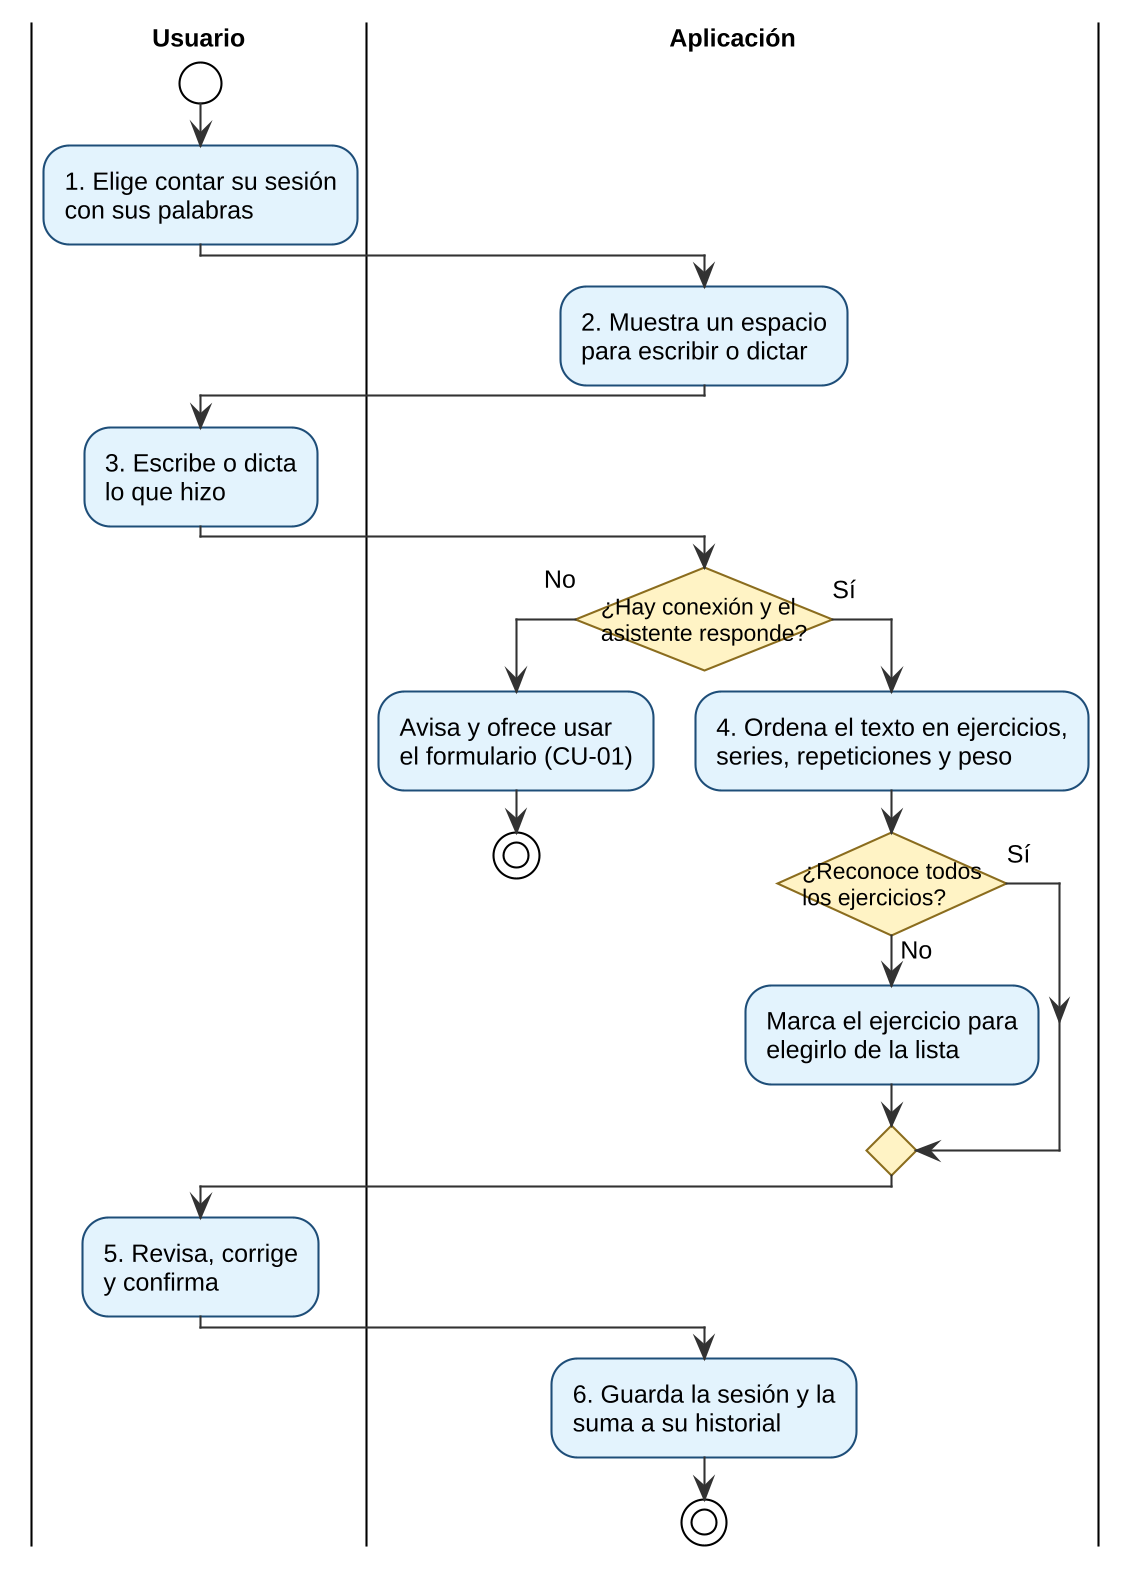
\includegraphics[width=0.78\textwidth,height=0.42\textheight,keepaspectratio]{figuras/diseno/dga_cu02.png}
    \captionof{figure}{Diagrama de Actividades -- CU-02: Contar mi sesión de fuerza con mis palabras.}
    \label{fig:dga_cu02}
\end{center}

\noindent\begin{minipage}{\linewidth}
\textbf{Descripción Esencial Expandida del Caso de Uso}
\par\vspace{0.2cm}
\noindent
{\renewcommand{\arraystretch}{1.25}\setstretch{1}\small
\begin{tabular}{|>{\raggedright\arraybackslash}p{2.9cm}|>{\raggedright\arraybackslash}p{12.1cm}|}
    \hline
    \rowcolor[HTML]{EFEFEF} \textbf{Propósito} & Registrar una sesión de fuerza escribiendo o dictando lo que se hizo, sin llenar un formulario. \\ \hline
    \textbf{Tipo} & Primario \\ \hline
    \textbf{Actores} & Atleta Híbrido, Asistente de inteligencia artificial \\ \hline
    \textbf{Requerimientos} & R01 \\ \hline
    \textbf{Precondiciones} & El usuario inició sesión y tiene el plan premium. Tiene conexión a Internet. \\ \hline
    \textbf{Poscondiciones} & La sesión confirmada queda en el historial del atleta y su carga queda actualizada. \\ \hline
\end{tabular}

\vspace{0.15cm}
\noindent
\begin{tabular}{|>{\raggedright\arraybackslash}p{7.5cm}|>{\raggedright\arraybackslash}p{7.5cm}|}
    \hline
    \rowcolor[HTML]{D9E1F2} \multicolumn{2}{|c|}{\textbf{Curso Normal de los Eventos}} \\ \hline
    \rowcolor[HTML]{EFEFEF} \multicolumn{1}{|c|}{\textbf{Usuario}} & \multicolumn{1}{c|}{\textbf{Respuesta del Sistema}} \\ \hline
        1. Elige contar su sesión con sus palabras. & 2. Muestra un espacio para escribir o dictar. \\ \hline
        3. Escribe o dicta lo que hizo, por ejemplo ``sentadilla, 4 series de 8 con 80 kilos''. & 4. Ordena el texto con ayuda del asistente de IA y muestra los ejercicios, las series, las repeticiones y el peso. \\ \hline
        5. Revisa el resultado, corrige lo que haga falta y lo confirma. & 6. Guarda la sesión y la suma a su historial. \\ \hline
    \rowcolor[HTML]{F2D9D9} \multicolumn{2}{|c|}{\textbf{Cursos Alternos}} \\ \hline
    \rowcolor[HTML]{EFEFEF} \multicolumn{1}{|c|}{\textbf{Usuario}} & \multicolumn{1}{c|}{\textbf{Respuesta del Sistema}} \\ \hline
         & 4. Si no reconoce un ejercicio, lo marca para que el atleta lo elija de la lista. \\ \hline
         & 4. Si no hay conexión o el asistente no responde, avisa y ofrece anotar la sesión con el formulario (CU-01). \\ \hline
\end{tabular}
}
\end{minipage}
\vspace{0.4cm}

\subsubsection{CU-03. Traer mis sesiones desde el reloj}

\textbf{Diagrama de Actividades}
\begin{center}
    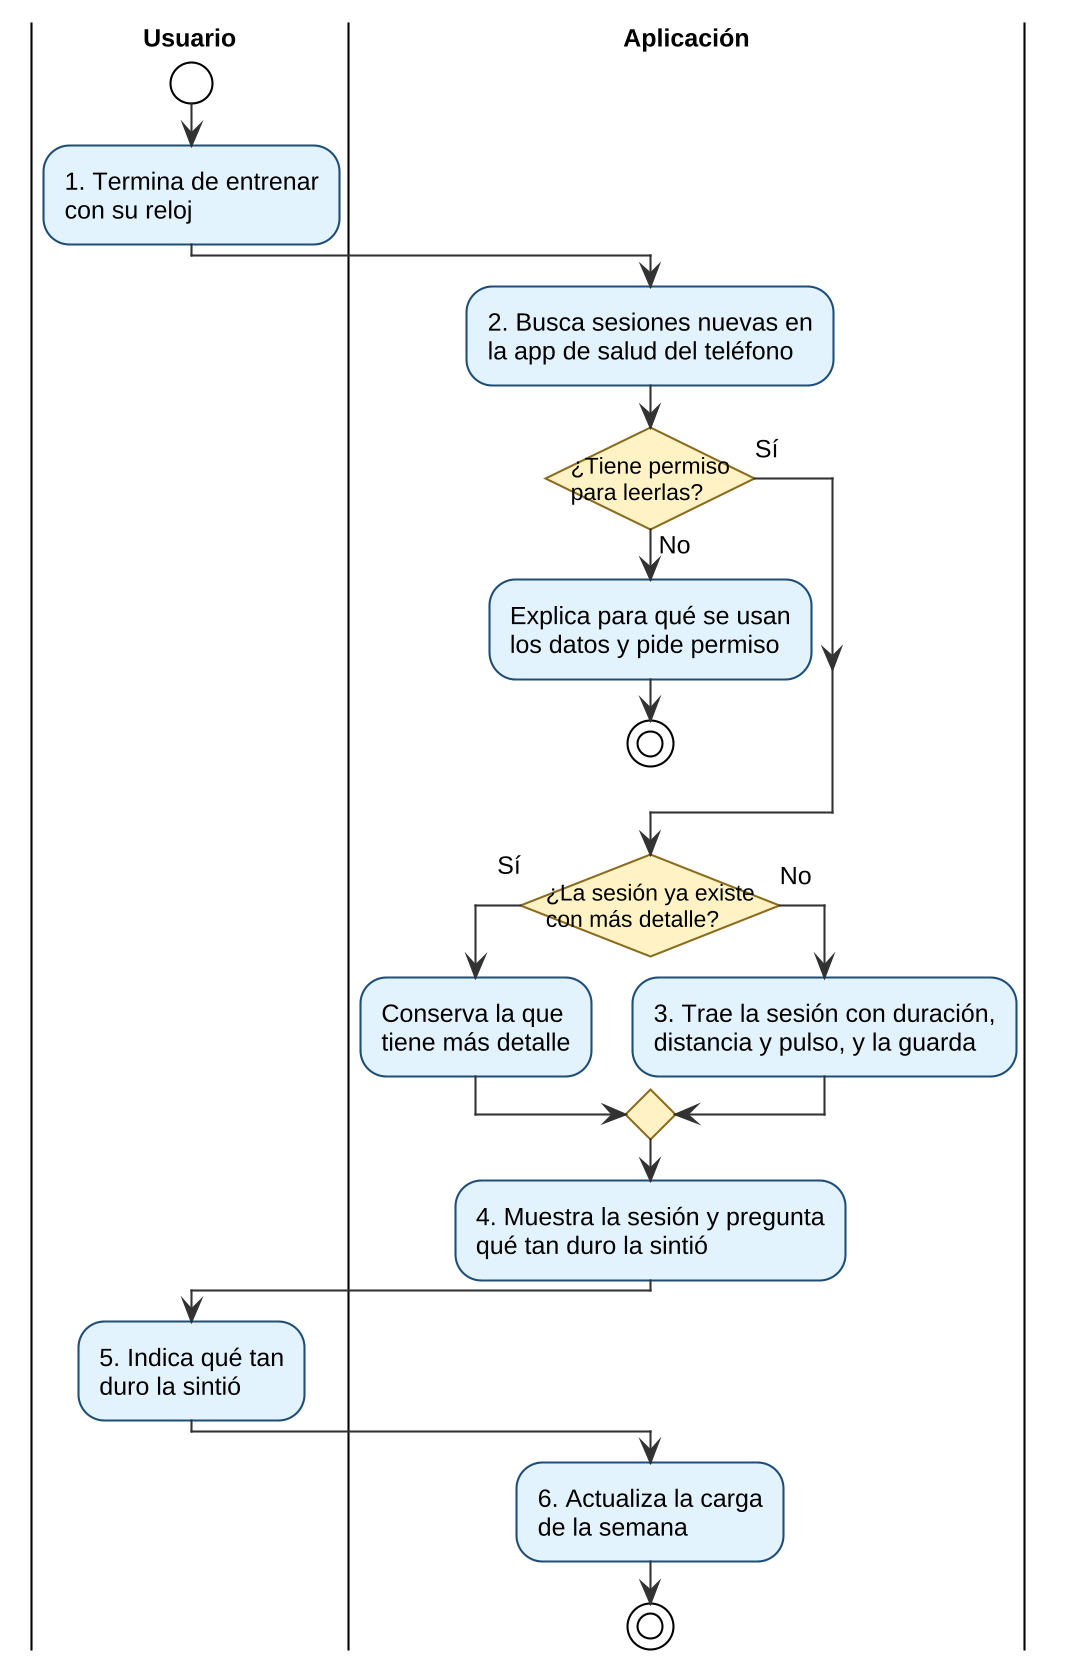
\includegraphics[width=0.78\textwidth,height=0.42\textheight,keepaspectratio]{figuras/diseno/dga_cu03.png}
    \captionof{figure}{Diagrama de Actividades -- CU-03: Traer mis sesiones desde el reloj.}
    \label{fig:dga_cu03}
\end{center}

\noindent\begin{minipage}{\linewidth}
\textbf{Descripción Esencial Expandida del Caso de Uso}
\par\vspace{0.2cm}
\noindent
{\renewcommand{\arraystretch}{1.25}\setstretch{1}\small
\begin{tabular}{|>{\raggedright\arraybackslash}p{2.9cm}|>{\raggedright\arraybackslash}p{12.1cm}|}
    \hline
    \rowcolor[HTML]{EFEFEF} \textbf{Propósito} & Registrar las sesiones de cardio hechas con un reloj, sin anotarlas a mano. \\ \hline
    \textbf{Tipo} & Primario \\ \hline
    \textbf{Actores} & Atleta Híbrido, App de salud del teléfono \\ \hline
    \textbf{Requerimientos} & R02 \\ \hline
    \textbf{Precondiciones} & El usuario inició sesión y tiene el plan premium. Su reloj está conectado a la app de salud del teléfono. \\ \hline
    \textbf{Poscondiciones} & La sesión queda en el historial del atleta y su carga queda actualizada. \\ \hline
\end{tabular}

\vspace{0.15cm}
\noindent
\begin{tabular}{|>{\raggedright\arraybackslash}p{7.5cm}|>{\raggedright\arraybackslash}p{7.5cm}|}
    \hline
    \rowcolor[HTML]{D9E1F2} \multicolumn{2}{|c|}{\textbf{Curso Normal de los Eventos}} \\ \hline
    \rowcolor[HTML]{EFEFEF} \multicolumn{1}{|c|}{\textbf{Usuario}} & \multicolumn{1}{c|}{\textbf{Respuesta del Sistema}} \\ \hline
        1. Termina de entrenar con su reloj. & 2. Busca sesiones nuevas en la app de salud del teléfono. \\ \hline
         & 3. Trae la sesión con su duración, su distancia y su pulso, y la guarda. \\ \hline
         & 4. Muestra la sesión en el historial y pregunta qué tan duro la sintió. \\ \hline
        5. Indica qué tan duro la sintió. & 6. Actualiza la carga de la semana. \\ \hline
    \rowcolor[HTML]{F2D9D9} \multicolumn{2}{|c|}{\textbf{Cursos Alternos}} \\ \hline
    \rowcolor[HTML]{EFEFEF} \multicolumn{1}{|c|}{\textbf{Usuario}} & \multicolumn{1}{c|}{\textbf{Respuesta del Sistema}} \\ \hline
         & 2. Si el atleta aún no da permiso, le explica para qué se usan esos datos y se lo pide. Sin permiso no lee nada. \\ \hline
         & 3. Si la misma sesión ya existe desde un archivo con más detalle, conserva la que tiene más detalle. \\ \hline
        5. Si no responde, la aplicación estima el esfuerzo con su pulso. &  \\ \hline
\end{tabular}
}
\end{minipage}
\vspace{0.4cm}

\subsubsection{CU-04. Subir el archivo de mi ciclocomputador}

\textbf{Diagrama de Actividades}
\begin{center}
    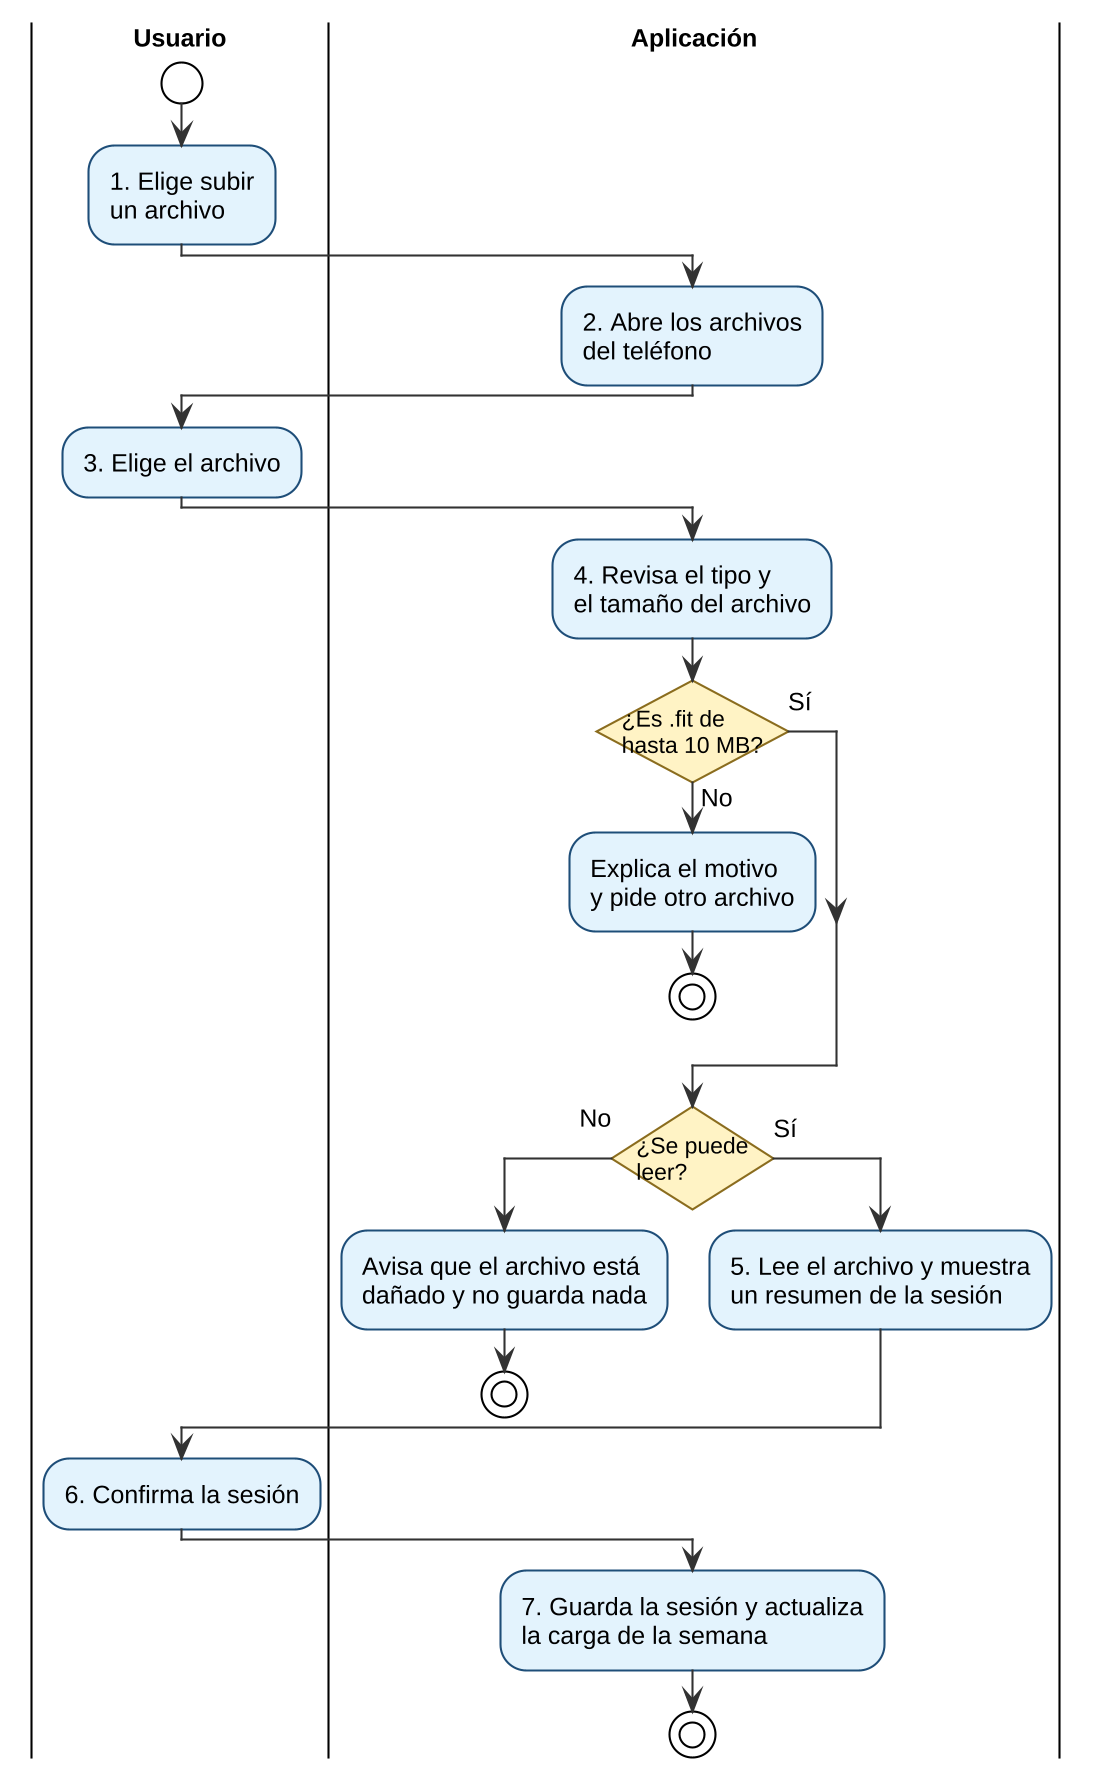
\includegraphics[width=0.78\textwidth,height=0.42\textheight,keepaspectratio]{figuras/diseno/dga_cu04.png}
    \captionof{figure}{Diagrama de Actividades -- CU-04: Subir el archivo de mi ciclocomputador.}
    \label{fig:dga_cu04}
\end{center}

\noindent\begin{minipage}{\linewidth}
\textbf{Descripción Esencial Expandida del Caso de Uso}
\par\vspace{0.2cm}
\noindent
{\renewcommand{\arraystretch}{1.25}\setstretch{1}\small
\begin{tabular}{|>{\raggedright\arraybackslash}p{2.9cm}|>{\raggedright\arraybackslash}p{12.1cm}|}
    \hline
    \rowcolor[HTML]{EFEFEF} \textbf{Propósito} & Incorporar una sesión con todo su detalle, como la potencia y la cadencia. \\ \hline
    \textbf{Tipo} & Primario \\ \hline
    \textbf{Actores} & Atleta Híbrido \\ \hline
    \textbf{Requerimientos} & R02 \\ \hline
    \textbf{Precondiciones} & El usuario inició sesión y tiene el plan premium. Tiene en su teléfono el archivo \texttt{.fit} exportado desde su dispositivo. \\ \hline
    \textbf{Poscondiciones} & La sesión queda en el historial del atleta, con el detalle del archivo. \\ \hline
\end{tabular}

\vspace{0.15cm}
\noindent
\begin{tabular}{|>{\raggedright\arraybackslash}p{7.5cm}|>{\raggedright\arraybackslash}p{7.5cm}|}
    \hline
    \rowcolor[HTML]{D9E1F2} \multicolumn{2}{|c|}{\textbf{Curso Normal de los Eventos}} \\ \hline
    \rowcolor[HTML]{EFEFEF} \multicolumn{1}{|c|}{\textbf{Usuario}} & \multicolumn{1}{c|}{\textbf{Respuesta del Sistema}} \\ \hline
        1. Elige subir un archivo. & 2. Abre los archivos del teléfono. \\ \hline
        3. Elige el archivo. & 4. Revisa que sea un archivo \texttt{.fit} de hasta 10 MB. \\ \hline
         & 5. Lee el archivo y muestra un resumen de la sesión. \\ \hline
        6. Confirma la sesión. & 7. Guarda la sesión y actualiza la carga de la semana. \\ \hline
    \rowcolor[HTML]{F2D9D9} \multicolumn{2}{|c|}{\textbf{Cursos Alternos}} \\ \hline
    \rowcolor[HTML]{EFEFEF} \multicolumn{1}{|c|}{\textbf{Usuario}} & \multicolumn{1}{c|}{\textbf{Respuesta del Sistema}} \\ \hline
         & 4. Si no es un archivo \texttt{.fit} o pesa más de 10 MB, explica el motivo y pide otro archivo. \\ \hline
         & 5. Si el archivo está dañado, avisa que no se pudo leer y no guarda nada. \\ \hline
\end{tabular}
}
\end{minipage}
\vspace{0.4cm}

\subsubsection{CU-05. Revisar mi fatiga y recibir alertas}

\textbf{Diagrama de Actividades}
\begin{center}
    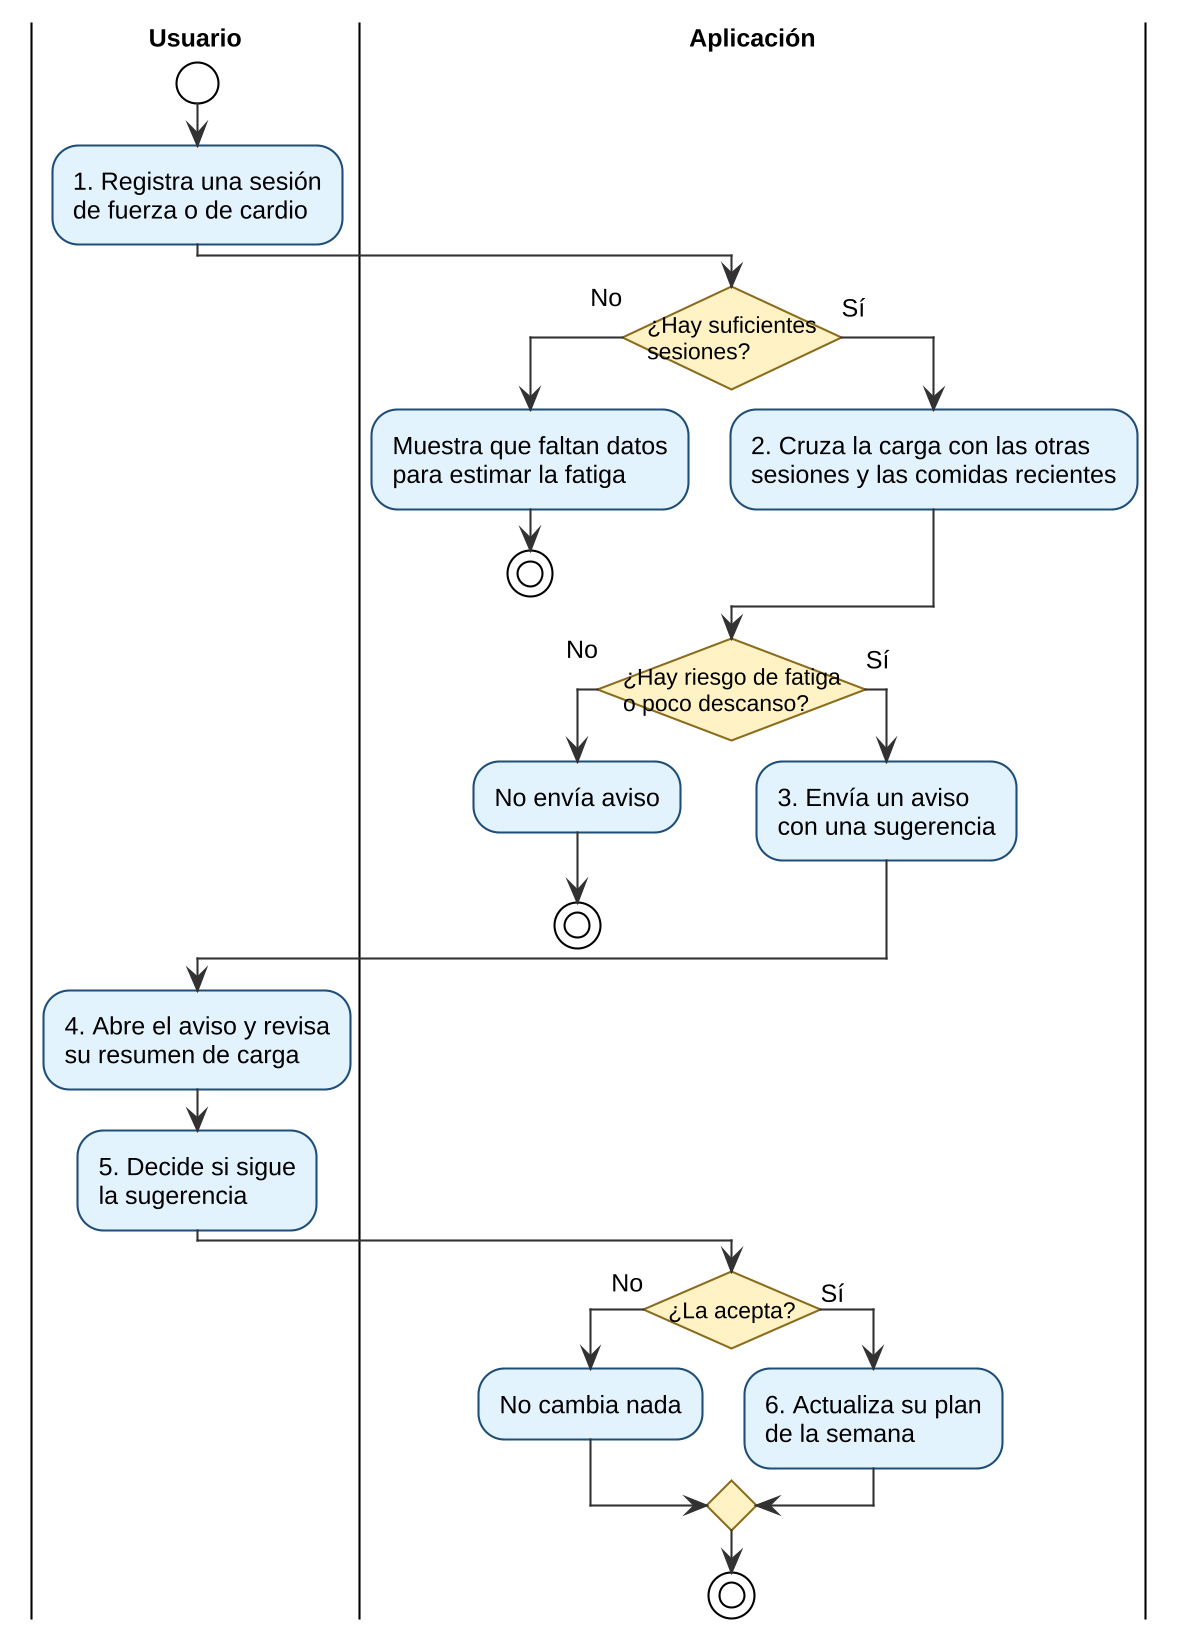
\includegraphics[width=0.78\textwidth,height=0.42\textheight,keepaspectratio]{figuras/diseno/dga_cu05.png}
    \captionof{figure}{Diagrama de Actividades -- CU-05: Revisar mi fatiga y recibir alertas.}
    \label{fig:dga_cu05}
\end{center}

\noindent\begin{minipage}{\linewidth}
\textbf{Descripción Esencial Expandida del Caso de Uso}
\par\vspace{0.2cm}
\noindent
{\renewcommand{\arraystretch}{1.25}\setstretch{1}\small
\begin{tabular}{|>{\raggedright\arraybackslash}p{2.9cm}|>{\raggedright\arraybackslash}p{12.1cm}|}
    \hline
    \rowcolor[HTML]{EFEFEF} \textbf{Propósito} & Avisar al atleta cuando puede estar acumulando demasiada fatiga, para que decida si ajusta su entrenamiento. \\ \hline
    \textbf{Tipo} & Primario \\ \hline
    \textbf{Actores} & Atleta Híbrido \\ \hline
    \textbf{Requerimientos} & R03 \\ \hline
    \textbf{Precondiciones} & El usuario inició sesión y tiene el plan premium. Tiene sesiones registradas. \\ \hline
    \textbf{Poscondiciones} & El atleta conoce su nivel de fatiga. Su entrenamiento solo cambia si él lo decide. \\ \hline
\end{tabular}

\vspace{0.15cm}
\noindent
\begin{tabular}{|>{\raggedright\arraybackslash}p{7.5cm}|>{\raggedright\arraybackslash}p{7.5cm}|}
    \hline
    \rowcolor[HTML]{D9E1F2} \multicolumn{2}{|c|}{\textbf{Curso Normal de los Eventos}} \\ \hline
    \rowcolor[HTML]{EFEFEF} \multicolumn{1}{|c|}{\textbf{Usuario}} & \multicolumn{1}{c|}{\textbf{Respuesta del Sistema}} \\ \hline
        1. Registra una sesión de fuerza o de cardio. & 2. Cruza la carga de la sesión con las otras sesiones y las comidas de los últimos días. \\ \hline
         & 3. Detecta un riesgo de fatiga o de poco descanso y envía un aviso con una sugerencia. \\ \hline
        4. Abre el aviso y revisa su resumen de carga. &  \\ \hline
        5. Decide si sigue la sugerencia. & 6. Si la acepta, actualiza su plan de la semana. \\ \hline
    \rowcolor[HTML]{F2D9D9} \multicolumn{2}{|c|}{\textbf{Cursos Alternos}} \\ \hline
    \rowcolor[HTML]{EFEFEF} \multicolumn{1}{|c|}{\textbf{Usuario}} & \multicolumn{1}{c|}{\textbf{Respuesta del Sistema}} \\ \hline
         & 2. Si todavía hay pocas sesiones, muestra que faltan datos para estimar la fatiga. \\ \hline
         & 3. Si no hay riesgo, no envía aviso. El atleta puede ver su resumen cuando quiera. \\ \hline
        5. Si ignora la sugerencia, la aplicación no cambia nada. &  \\ \hline
\end{tabular}
}
\end{minipage}
\vspace{0.4cm}

\subsubsection{CU-06. Anotar una comida buscando los alimentos}

\textbf{Diagrama de Actividades}
\begin{center}
    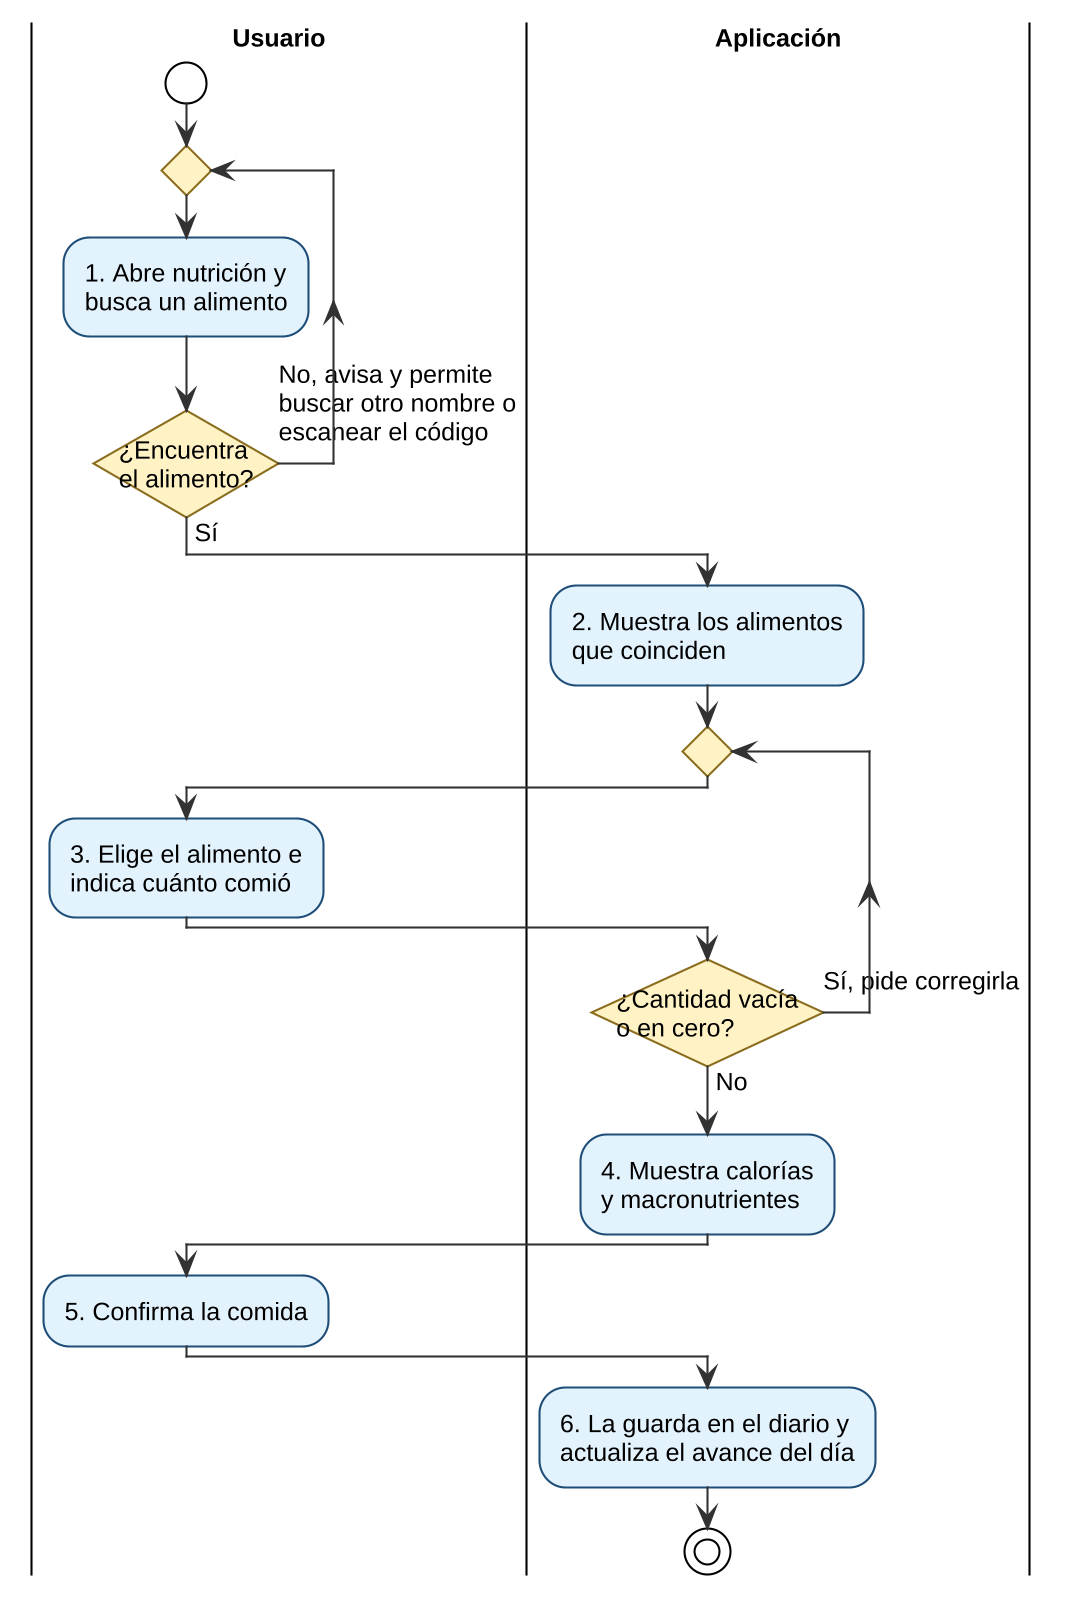
\includegraphics[width=0.78\textwidth,height=0.42\textheight,keepaspectratio]{figuras/diseno/dga_cu06.png}
    \captionof{figure}{Diagrama de Actividades -- CU-06: Anotar una comida buscando los alimentos.}
    \label{fig:dga_cu06}
\end{center}

\noindent\begin{minipage}{\linewidth}
\textbf{Descripción Esencial Expandida del Caso de Uso}
\par\vspace{0.2cm}
\noindent
{\renewcommand{\arraystretch}{1.25}\setstretch{1}\small
\begin{tabular}{|>{\raggedright\arraybackslash}p{2.9cm}|>{\raggedright\arraybackslash}p{12.1cm}|}
    \hline
    \rowcolor[HTML]{EFEFEF} \textbf{Propósito} & Registrar una comida eligiendo los alimentos desde una lista. \\ \hline
    \textbf{Tipo} & Primario \\ \hline
    \textbf{Actores} & Atleta Básico, Atleta Híbrido \\ \hline
    \textbf{Requerimientos} & R04 \\ \hline
    \textbf{Precondiciones} & El usuario inició sesión en la aplicación. \\ \hline
    \textbf{Poscondiciones} & La comida queda en el diario del día. \\ \hline
\end{tabular}

\vspace{0.15cm}
\noindent
\begin{tabular}{|>{\raggedright\arraybackslash}p{7.5cm}|>{\raggedright\arraybackslash}p{7.5cm}|}
    \hline
    \rowcolor[HTML]{D9E1F2} \multicolumn{2}{|c|}{\textbf{Curso Normal de los Eventos}} \\ \hline
    \rowcolor[HTML]{EFEFEF} \multicolumn{1}{|c|}{\textbf{Usuario}} & \multicolumn{1}{c|}{\textbf{Respuesta del Sistema}} \\ \hline
        1. Abre el módulo de nutrición y busca un alimento. & 2. Muestra los alimentos que coinciden. \\ \hline
        3. Elige el alimento e indica cuánto comió. & 4. Muestra sus calorías y sus macronutrientes. \\ \hline
        5. Confirma la comida. & 6. La guarda en el diario y actualiza el avance del día. \\ \hline
    \rowcolor[HTML]{F2D9D9} \multicolumn{2}{|c|}{\textbf{Cursos Alternos}} \\ \hline
    \rowcolor[HTML]{EFEFEF} \multicolumn{1}{|c|}{\textbf{Usuario}} & \multicolumn{1}{c|}{\textbf{Respuesta del Sistema}} \\ \hline
         & 2. Si no encuentra el alimento, avisa y permite buscar con otro nombre o escanear su código de barras (CU-15). \\ \hline
        3. Si la cantidad está vacía o es cero, la aplicación pide corregirla antes de seguir. &  \\ \hline
\end{tabular}
}
\end{minipage}
\vspace{0.4cm}

\subsubsection{CU-07. Registrar una comida con una foto}

\textbf{Diagrama de Actividades}
\begin{center}
    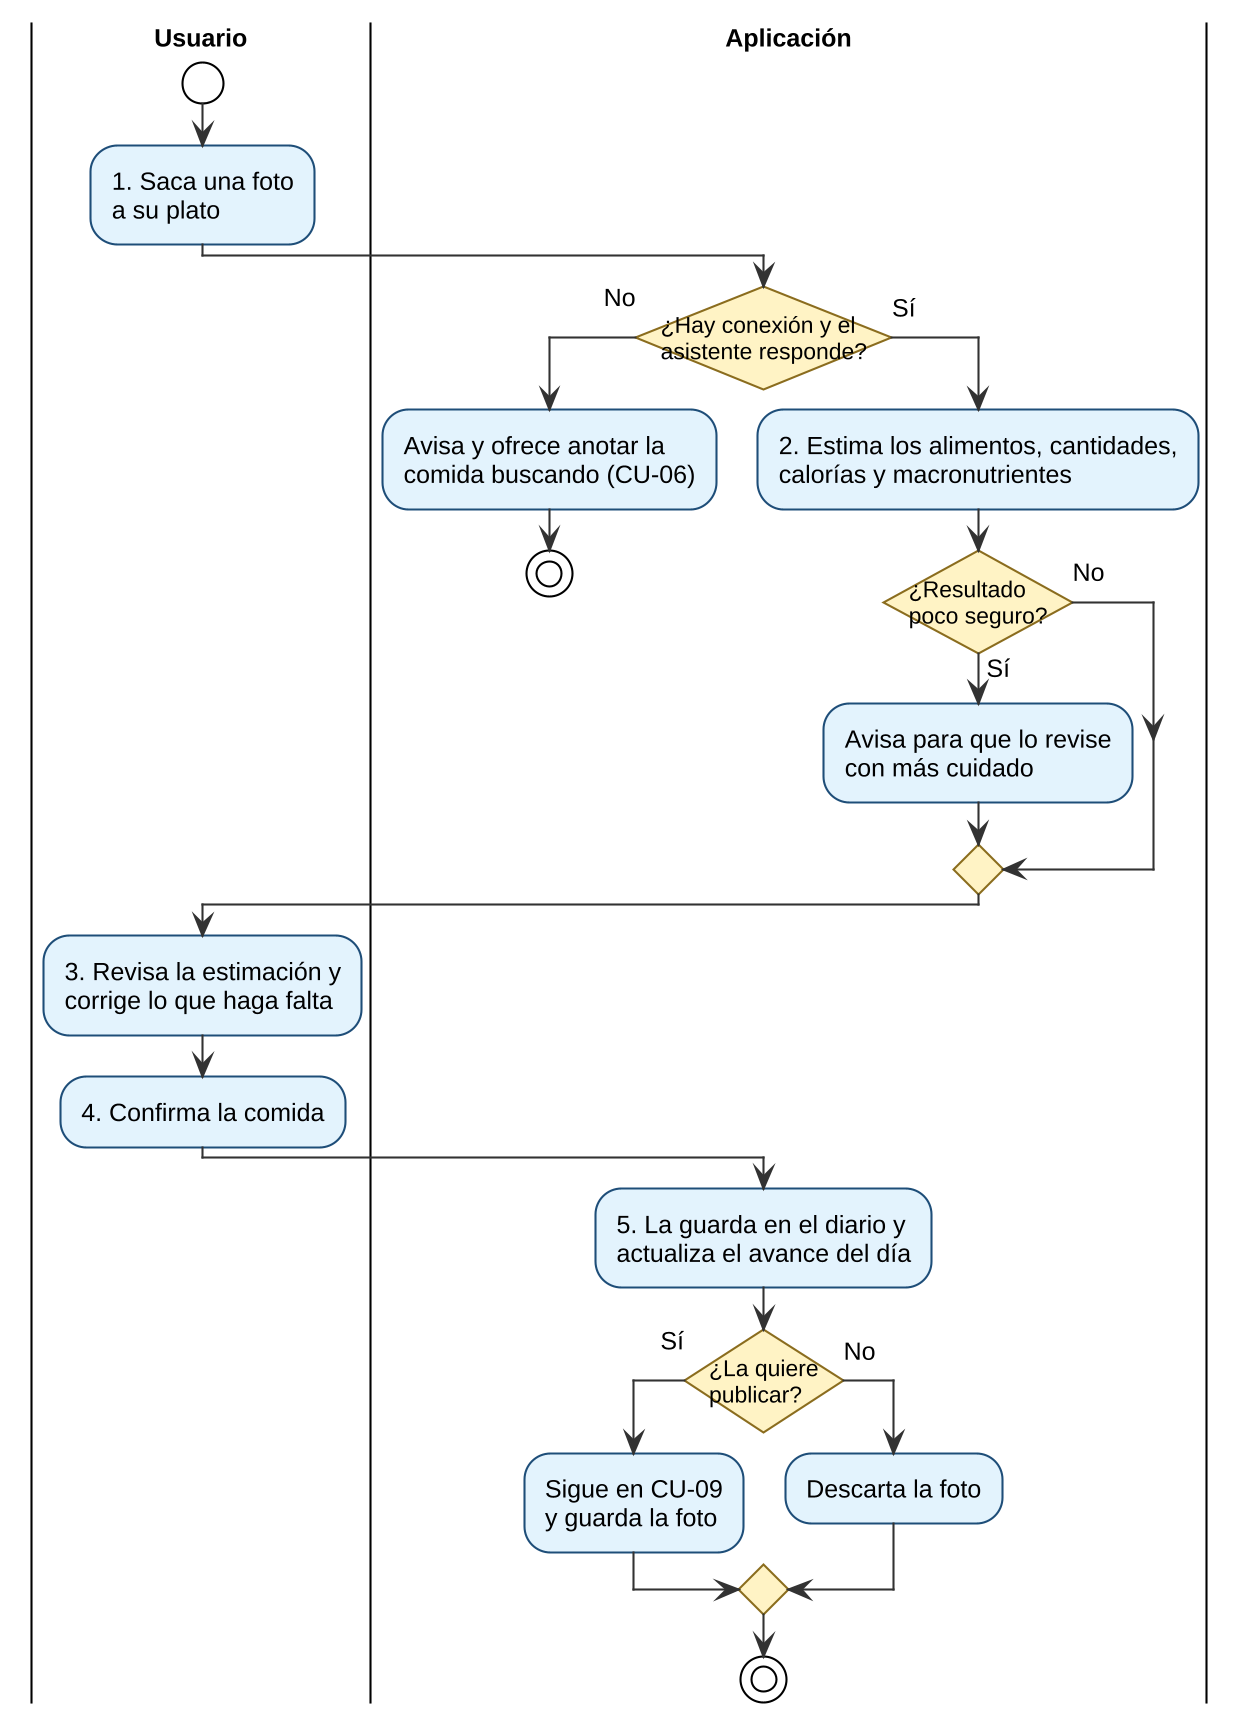
\includegraphics[width=0.78\textwidth,height=0.42\textheight,keepaspectratio]{figuras/diseno/dga_cu07.png}
    \captionof{figure}{Diagrama de Actividades -- CU-07: Registrar una comida con una foto.}
    \label{fig:dga_cu07}
\end{center}

\noindent\begin{minipage}{\linewidth}
\textbf{Descripción Esencial Expandida del Caso de Uso}
\par\vspace{0.2cm}
\noindent
{\renewcommand{\arraystretch}{1.25}\setstretch{1}\small
\begin{tabular}{|>{\raggedright\arraybackslash}p{2.9cm}|>{\raggedright\arraybackslash}p{12.1cm}|}
    \hline
    \rowcolor[HTML]{EFEFEF} \textbf{Propósito} & Registrar una comida sacándole una foto al plato, para no buscar cada alimento. \\ \hline
    \textbf{Tipo} & Primario \\ \hline
    \textbf{Actores} & Atleta Híbrido, Asistente de inteligencia artificial \\ \hline
    \textbf{Requerimientos} & R04 \\ \hline
    \textbf{Precondiciones} & El usuario inició sesión y tiene el plan premium. Tiene conexión a Internet. \\ \hline
    \textbf{Poscondiciones} & La comida confirmada queda en el diario del día. \\ \hline
\end{tabular}

\vspace{0.15cm}
\noindent
\begin{tabular}{|>{\raggedright\arraybackslash}p{7.5cm}|>{\raggedright\arraybackslash}p{7.5cm}|}
    \hline
    \rowcolor[HTML]{D9E1F2} \multicolumn{2}{|c|}{\textbf{Curso Normal de los Eventos}} \\ \hline
    \rowcolor[HTML]{EFEFEF} \multicolumn{1}{|c|}{\textbf{Usuario}} & \multicolumn{1}{c|}{\textbf{Respuesta del Sistema}} \\ \hline
        1. Saca una foto a su plato. & 2. Estima con ayuda del asistente de IA los alimentos, las cantidades, las calorías y los macronutrientes, y los muestra. \\ \hline
        3. Revisa la estimación y corrige lo que haga falta. &  \\ \hline
        4. Confirma la comida. & 5. La guarda en el diario, actualiza el avance del día y descarta la foto. \\ \hline
    \rowcolor[HTML]{F2D9D9} \multicolumn{2}{|c|}{\textbf{Cursos Alternos}} \\ \hline
    \rowcolor[HTML]{EFEFEF} \multicolumn{1}{|c|}{\textbf{Usuario}} & \multicolumn{1}{c|}{\textbf{Respuesta del Sistema}} \\ \hline
         & 2. Si el resultado es poco seguro, avisa al atleta para que lo revise con más cuidado. \\ \hline
         & 2. Si no hay conexión o el asistente no responde, avisa y ofrece anotar la comida buscando los alimentos (CU-06). \\ \hline
        4. Si quiere compartir el plato, puede publicarlo (CU-09). En ese caso la foto sí se guarda. &  \\ \hline
\end{tabular}
}
\end{minipage}
\vspace{0.4cm}

\subsubsection{CU-08. Agregar una receta ajustada a mis metas}

\textbf{Diagrama de Actividades}
\begin{center}
    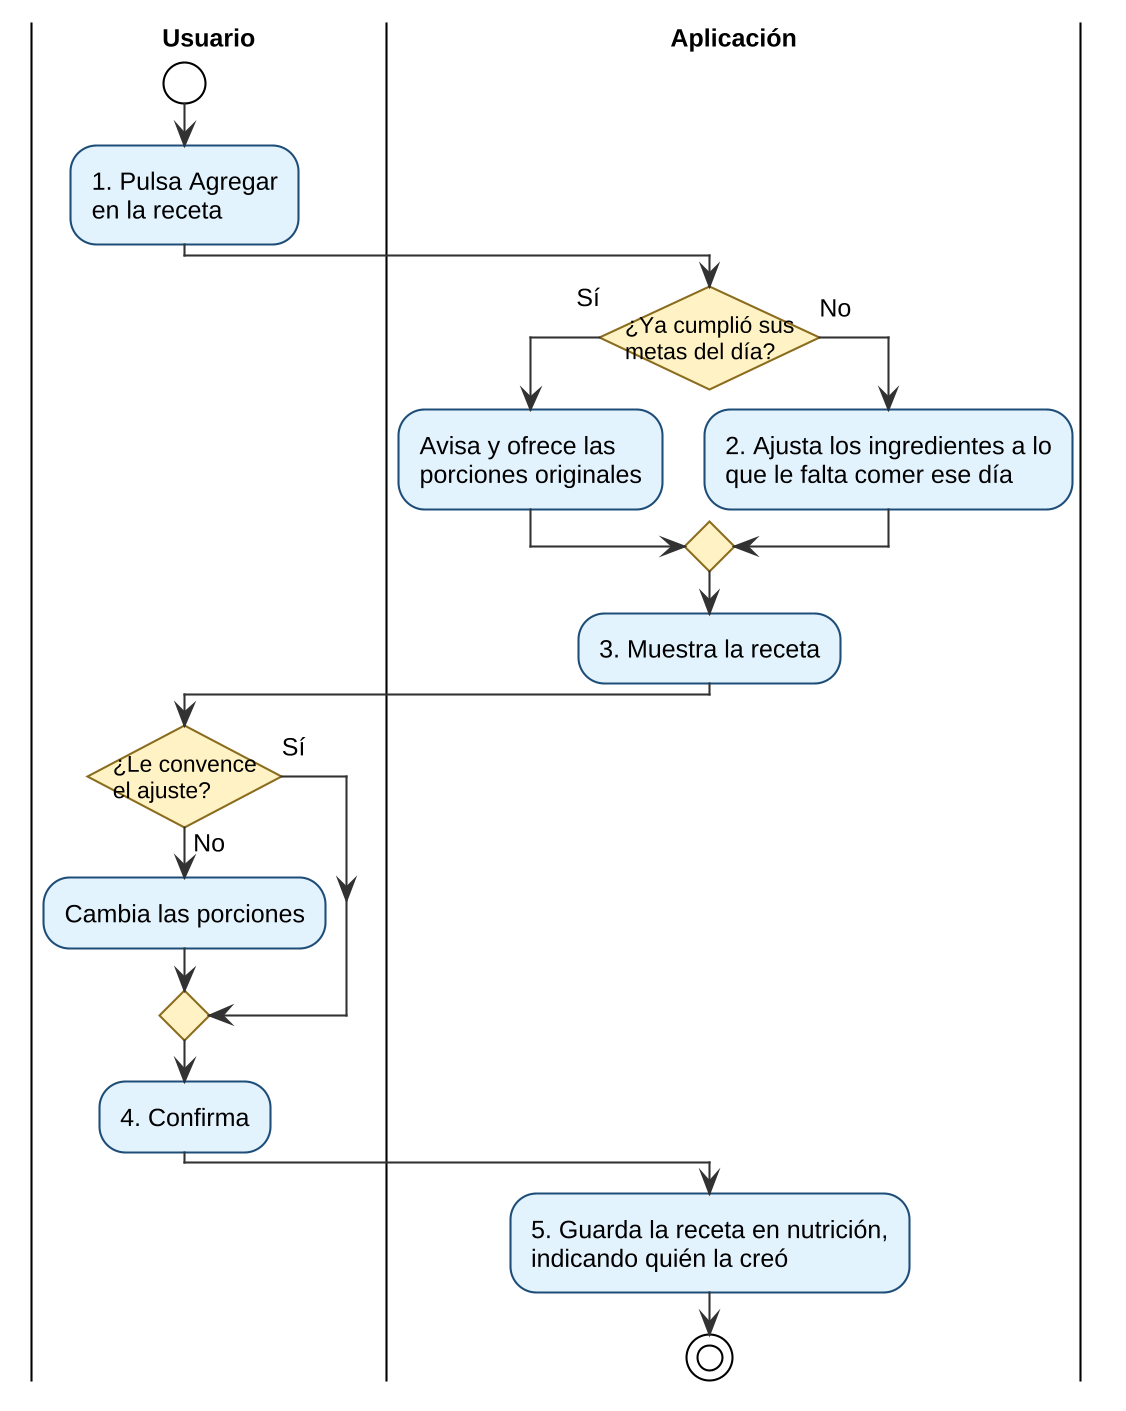
\includegraphics[width=0.78\textwidth,height=0.42\textheight,keepaspectratio]{figuras/diseno/dga_cu08.png}
    \captionof{figure}{Diagrama de Actividades -- CU-08: Agregar una receta ajustada a mis metas.}
    \label{fig:dga_cu08}
\end{center}

\noindent\begin{minipage}{\linewidth}
\textbf{Descripción Esencial Expandida del Caso de Uso}
\par\vspace{0.2cm}
\noindent
{\renewcommand{\arraystretch}{1.25}\setstretch{1}\small
\begin{tabular}{|>{\raggedright\arraybackslash}p{2.9cm}|>{\raggedright\arraybackslash}p{12.1cm}|}
    \hline
    \rowcolor[HTML]{EFEFEF} \textbf{Propósito} & Llevar una receta de otra persona al módulo de nutrición, con porciones adaptadas a lo que el atleta necesita ese día. \\ \hline
    \textbf{Tipo} & Primario \\ \hline
    \textbf{Actores} & Atleta Híbrido \\ \hline
    \textbf{Requerimientos} & R12 \\ \hline
    \textbf{Precondiciones} & El usuario inició sesión y tiene el plan premium. Ve una receta en su muro. \\ \hline
    \textbf{Poscondiciones} & La receta queda en el módulo de nutrición. No se registra como comida hasta que el atleta la anote en su diario. \\ \hline
\end{tabular}

\vspace{0.15cm}
\noindent
\begin{tabular}{|>{\raggedright\arraybackslash}p{7.5cm}|>{\raggedright\arraybackslash}p{7.5cm}|}
    \hline
    \rowcolor[HTML]{D9E1F2} \multicolumn{2}{|c|}{\textbf{Curso Normal de los Eventos}} \\ \hline
    \rowcolor[HTML]{EFEFEF} \multicolumn{1}{|c|}{\textbf{Usuario}} & \multicolumn{1}{c|}{\textbf{Respuesta del Sistema}} \\ \hline
        1. Pulsa Agregar en la receta. & 2. Revisa lo que le falta comer ese día y ajusta la cantidad de cada ingrediente, manteniendo las proporciones. \\ \hline
         & 3. Muestra la receta ajustada. \\ \hline
        4. Confirma. & 5. Guarda la receta en su módulo de nutrición, indicando quién la creó. \\ \hline
    \rowcolor[HTML]{F2D9D9} \multicolumn{2}{|c|}{\textbf{Cursos Alternos}} \\ \hline
    \rowcolor[HTML]{EFEFEF} \multicolumn{1}{|c|}{\textbf{Usuario}} & \multicolumn{1}{c|}{\textbf{Respuesta del Sistema}} \\ \hline
         & 2. Si ya cumplió sus metas del día, avisa y ofrece guardar la receta con sus porciones originales. \\ \hline
        4. Si no le convence el ajuste, puede cambiar las porciones antes de confirmar. &  \\ \hline
\end{tabular}
}
\end{minipage}
\vspace{0.4cm}

\subsubsection{CU-09. Publicar una sesión, ruta o comida}

\textbf{Diagrama de Actividades}
\begin{center}
    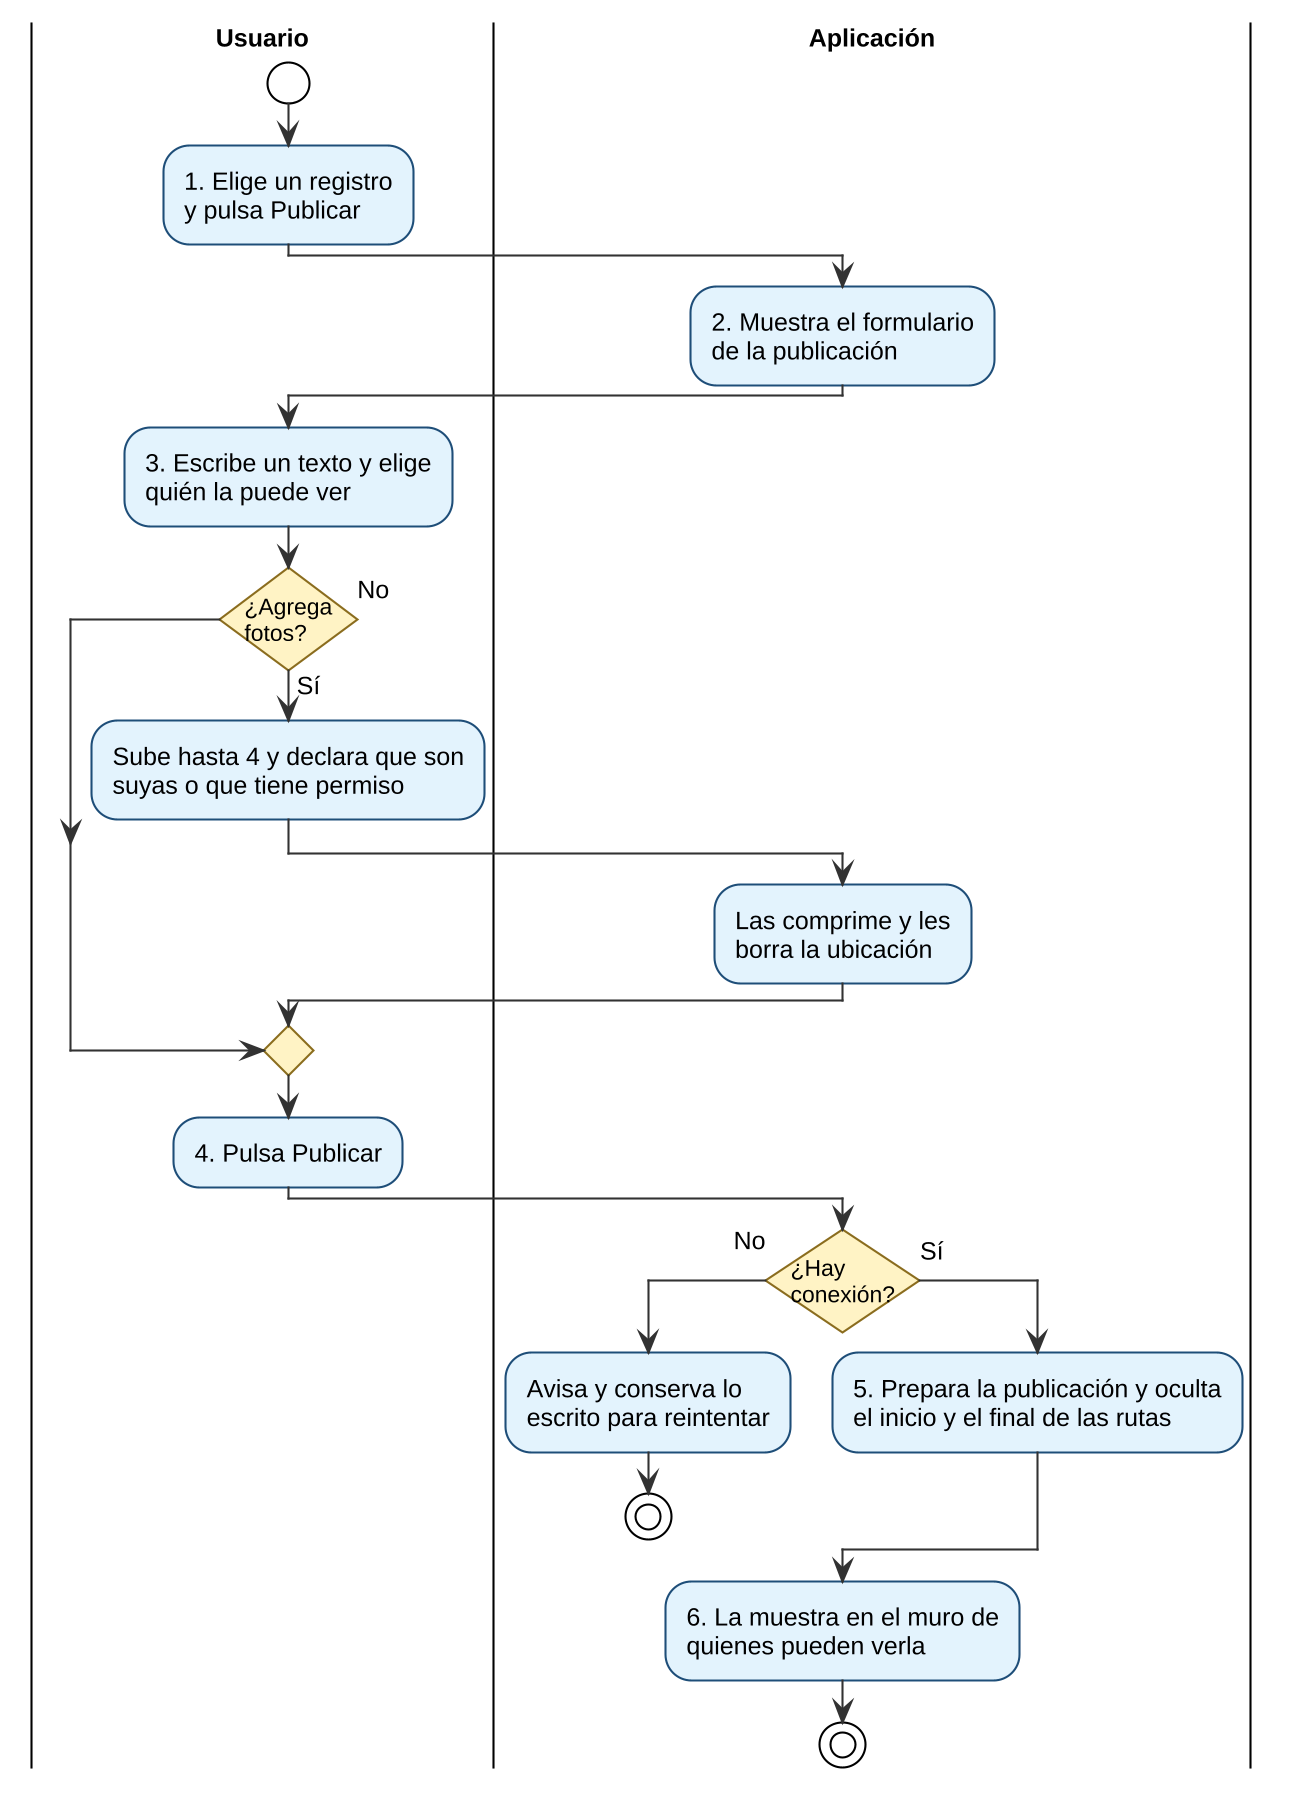
\includegraphics[width=0.78\textwidth,height=0.42\textheight,keepaspectratio]{figuras/diseno/dga_cu09.png}
    \captionof{figure}{Diagrama de Actividades -- CU-09: Publicar una sesión, ruta o comida.}
    \label{fig:dga_cu09}
\end{center}

\noindent\begin{minipage}{\linewidth}
\textbf{Descripción Esencial Expandida del Caso de Uso}
\par\vspace{0.2cm}
\noindent
{\renewcommand{\arraystretch}{1.25}\setstretch{1}\small
\begin{tabular}{|>{\raggedright\arraybackslash}p{2.9cm}|>{\raggedright\arraybackslash}p{12.1cm}|}
    \hline
    \rowcolor[HTML]{EFEFEF} \textbf{Propósito} & Compartir con la comunidad algo que el atleta ya registró o creó, como una receta propia (CU-27). \\ \hline
    \textbf{Tipo} & Primario \\ \hline
    \textbf{Actores} & Atleta Híbrido \\ \hline
    \textbf{Requerimientos} & R08, R15 \\ \hline
    \textbf{Precondiciones} & El usuario inició sesión y tiene el plan premium. Tiene al menos un registro guardado. \\ \hline
    \textbf{Poscondiciones} & La publicación queda visible solo para quienes el atleta eligió. \\ \hline
\end{tabular}

\vspace{0.15cm}
\noindent
\begin{tabular}{|>{\raggedright\arraybackslash}p{7.5cm}|>{\raggedright\arraybackslash}p{7.5cm}|}
    \hline
    \rowcolor[HTML]{D9E1F2} \multicolumn{2}{|c|}{\textbf{Curso Normal de los Eventos}} \\ \hline
    \rowcolor[HTML]{EFEFEF} \multicolumn{1}{|c|}{\textbf{Usuario}} & \multicolumn{1}{c|}{\textbf{Respuesta del Sistema}} \\ \hline
        1. Elige un registro (una sesión, una ruta, una comida o una receta) y pulsa Publicar. & 2. Muestra el formulario de la publicación. \\ \hline
        3. Escribe un texto y elige quién la puede ver (todos, sus seguidores o solo él). &  \\ \hline
        4. Pulsa Publicar. & 5. Prepara la publicación. Si es una ruta, oculta el inicio y el final del recorrido. \\ \hline
         & 6. Muestra la publicación en el muro de quienes pueden verla. \\ \hline
    \rowcolor[HTML]{F2D9D9} \multicolumn{2}{|c|}{\textbf{Cursos Alternos}} \\ \hline
    \rowcolor[HTML]{EFEFEF} \multicolumn{1}{|c|}{\textbf{Usuario}} & \multicolumn{1}{c|}{\textbf{Respuesta del Sistema}} \\ \hline
        3. Si agrega fotos, puede subir hasta 4 y declara que son suyas o que tiene permiso. La aplicación las comprime y les borra la ubicación. &  \\ \hline
        3. Si intenta agregar más de 4 fotos, la aplicación no lo permite y le avisa. &  \\ \hline
         & 5. Si se corta la conexión, avisa que no se pudo publicar y conserva lo escrito para reintentar. \\ \hline
\end{tabular}
}
\end{minipage}
\vspace{0.4cm}

\subsubsection{CU-10. Mantener el catálogo de ejercicios}

\textbf{Diagrama de Actividades}
\begin{center}
    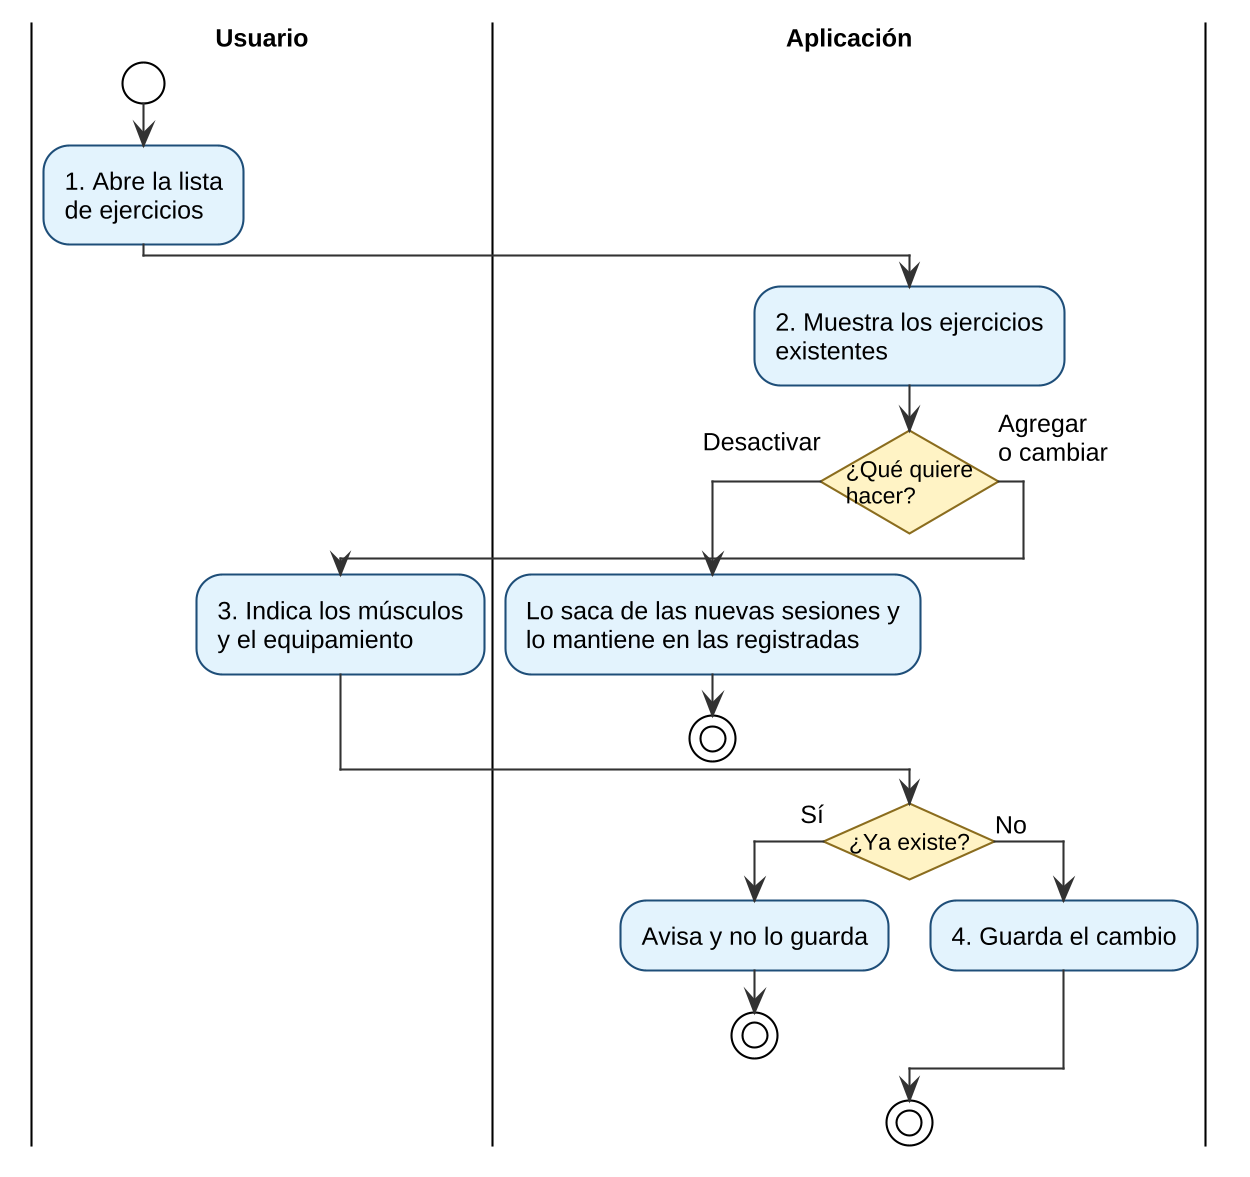
\includegraphics[width=0.78\textwidth,height=0.42\textheight,keepaspectratio]{figuras/diseno/dga_cu10.png}
    \captionof{figure}{Diagrama de Actividades -- CU-10: Mantener el catálogo de ejercicios.}
    \label{fig:dga_cu10}
\end{center}

\noindent\begin{minipage}{\linewidth}
\textbf{Descripción Esencial Expandida del Caso de Uso}
\par\vspace{0.2cm}
\noindent
{\renewcommand{\arraystretch}{1.25}\setstretch{1}\small
\begin{tabular}{|>{\raggedright\arraybackslash}p{2.9cm}|>{\raggedright\arraybackslash}p{12.1cm}|}
    \hline
    \rowcolor[HTML]{EFEFEF} \textbf{Propósito} & Mantener al día la lista de ejercicios que usan los atletas. \\ \hline
    \textbf{Tipo} & Primario \\ \hline
    \textbf{Actores} & Administrador \\ \hline
    \textbf{Requerimientos} & R11 \\ \hline
    \textbf{Precondiciones} & El administrador inició sesión en el panel de administración. \\ \hline
    \textbf{Poscondiciones} & La lista de ejercicios queda actualizada para todos los atletas. \\ \hline
\end{tabular}

\vspace{0.15cm}
\noindent
\begin{tabular}{|>{\raggedright\arraybackslash}p{7.5cm}|>{\raggedright\arraybackslash}p{7.5cm}|}
    \hline
    \rowcolor[HTML]{D9E1F2} \multicolumn{2}{|c|}{\textbf{Curso Normal de los Eventos}} \\ \hline
    \rowcolor[HTML]{EFEFEF} \multicolumn{1}{|c|}{\textbf{Usuario}} & \multicolumn{1}{c|}{\textbf{Respuesta del Sistema}} \\ \hline
        1. Abre la lista de ejercicios. & 2. Muestra los ejercicios existentes. \\ \hline
        3. Agrega o cambia un ejercicio, indicando qué músculos trabaja y qué equipamiento necesita. & 4. Revisa que no esté repetido y guarda el cambio. \\ \hline
    \rowcolor[HTML]{F2D9D9} \multicolumn{2}{|c|}{\textbf{Cursos Alternos}} \\ \hline
    \rowcolor[HTML]{EFEFEF} \multicolumn{1}{|c|}{\textbf{Usuario}} & \multicolumn{1}{c|}{\textbf{Respuesta del Sistema}} \\ \hline
        3. Si desactiva un ejercicio, este deja de aparecer para nuevas sesiones, pero se mantiene en las ya registradas. &  \\ \hline
         & 4. Si el ejercicio ya existe, avisa y no lo guarda. \\ \hline
\end{tabular}
}
\end{minipage}
\vspace{0.4cm}

\subsubsection{CU-11. Revisar el contenido reportado}

\textbf{Diagrama de Actividades}
\begin{center}
    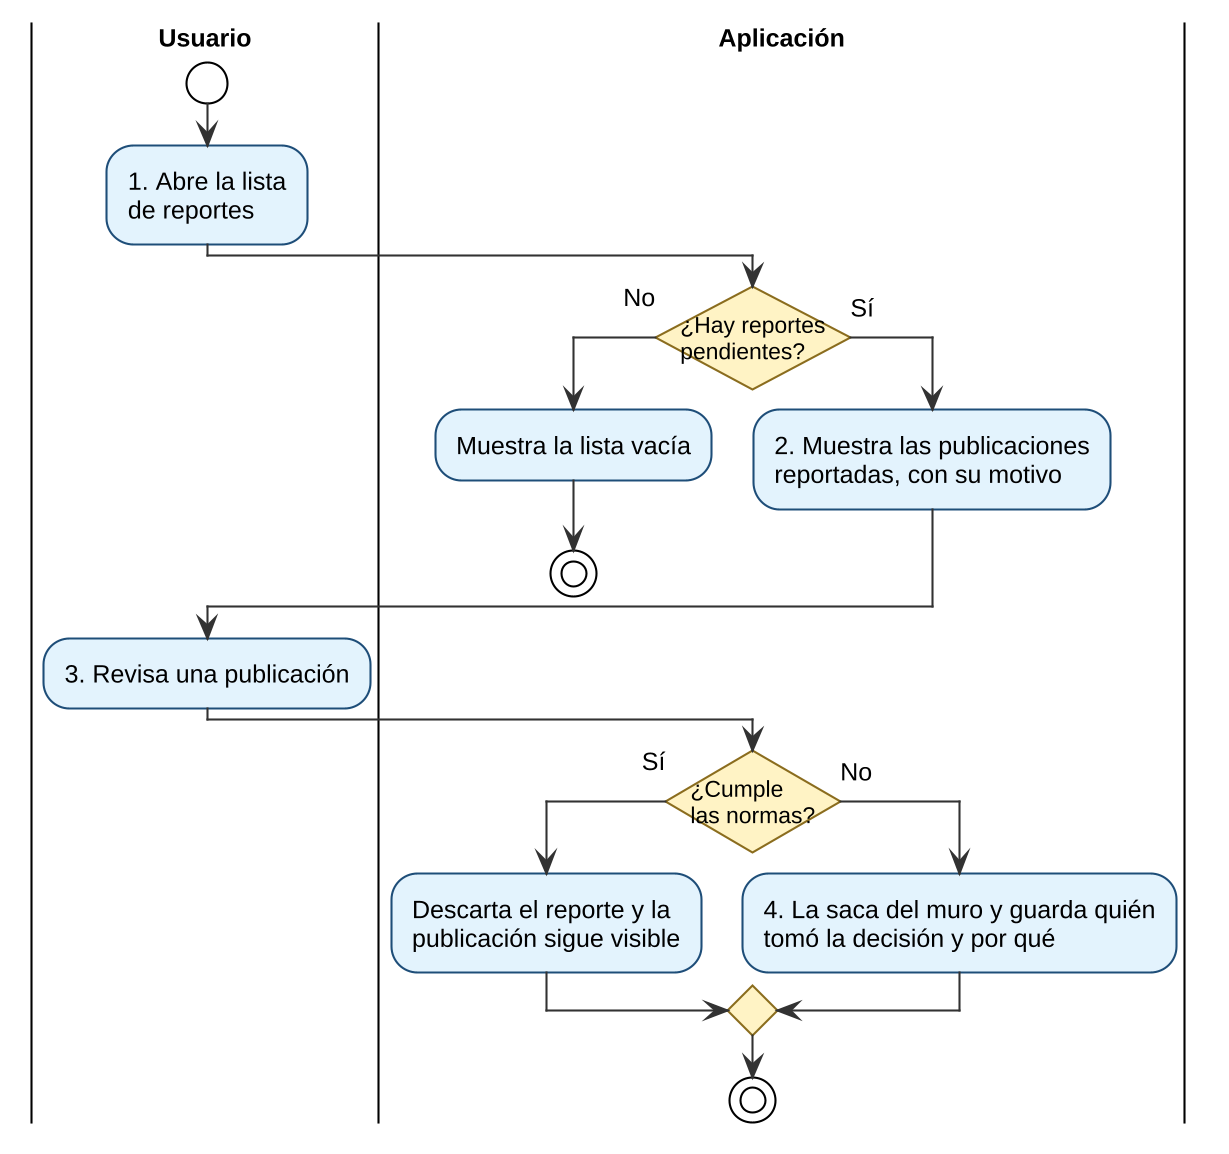
\includegraphics[width=0.78\textwidth,height=0.42\textheight,keepaspectratio]{figuras/diseno/dga_cu11.png}
    \captionof{figure}{Diagrama de Actividades -- CU-11: Revisar el contenido reportado.}
    \label{fig:dga_cu11}
\end{center}

\noindent\begin{minipage}{\linewidth}
\textbf{Descripción Esencial Expandida del Caso de Uso}
\par\vspace{0.2cm}
\noindent
{\renewcommand{\arraystretch}{1.25}\setstretch{1}\small
\begin{tabular}{|>{\raggedright\arraybackslash}p{2.9cm}|>{\raggedright\arraybackslash}p{12.1cm}|}
    \hline
    \rowcolor[HTML]{EFEFEF} \textbf{Propósito} & Retirar de la comunidad lo que no cumpla las normas o pueda ser peligroso para la salud. \\ \hline
    \textbf{Tipo} & Primario \\ \hline
    \textbf{Actores} & Administrador \\ \hline
    \textbf{Requerimientos} & R11 \\ \hline
    \textbf{Precondiciones} & El administrador inició sesión en el panel de administración. \\ \hline
    \textbf{Poscondiciones} & El reporte queda resuelto y hay registro de la decisión. \\ \hline
\end{tabular}

\vspace{0.15cm}
\noindent
\begin{tabular}{|>{\raggedright\arraybackslash}p{7.5cm}|>{\raggedright\arraybackslash}p{7.5cm}|}
    \hline
    \rowcolor[HTML]{D9E1F2} \multicolumn{2}{|c|}{\textbf{Curso Normal de los Eventos}} \\ \hline
    \rowcolor[HTML]{EFEFEF} \multicolumn{1}{|c|}{\textbf{Usuario}} & \multicolumn{1}{c|}{\textbf{Respuesta del Sistema}} \\ \hline
        1. Abre la lista de reportes. & 2. Muestra las publicaciones reportadas, con su motivo. \\ \hline
        3. Revisa una publicación y decide ocultarla. & 4. La saca del muro y guarda quién tomó la decisión y por qué. \\ \hline
    \rowcolor[HTML]{F2D9D9} \multicolumn{2}{|c|}{\textbf{Cursos Alternos}} \\ \hline
    \rowcolor[HTML]{EFEFEF} \multicolumn{1}{|c|}{\textbf{Usuario}} & \multicolumn{1}{c|}{\textbf{Respuesta del Sistema}} \\ \hline
         & 2. Si no hay reportes pendientes, muestra la lista vacía. \\ \hline
        3. Si la publicación cumple las normas, descarta el reporte y la publicación sigue visible. &  \\ \hline
\end{tabular}
}
\end{minipage}
\vspace{0.4cm}

\subsubsection{CU-12. Completar mi perfil y recibir un plan semanal}

\textbf{Diagrama de Actividades}
\begin{center}
    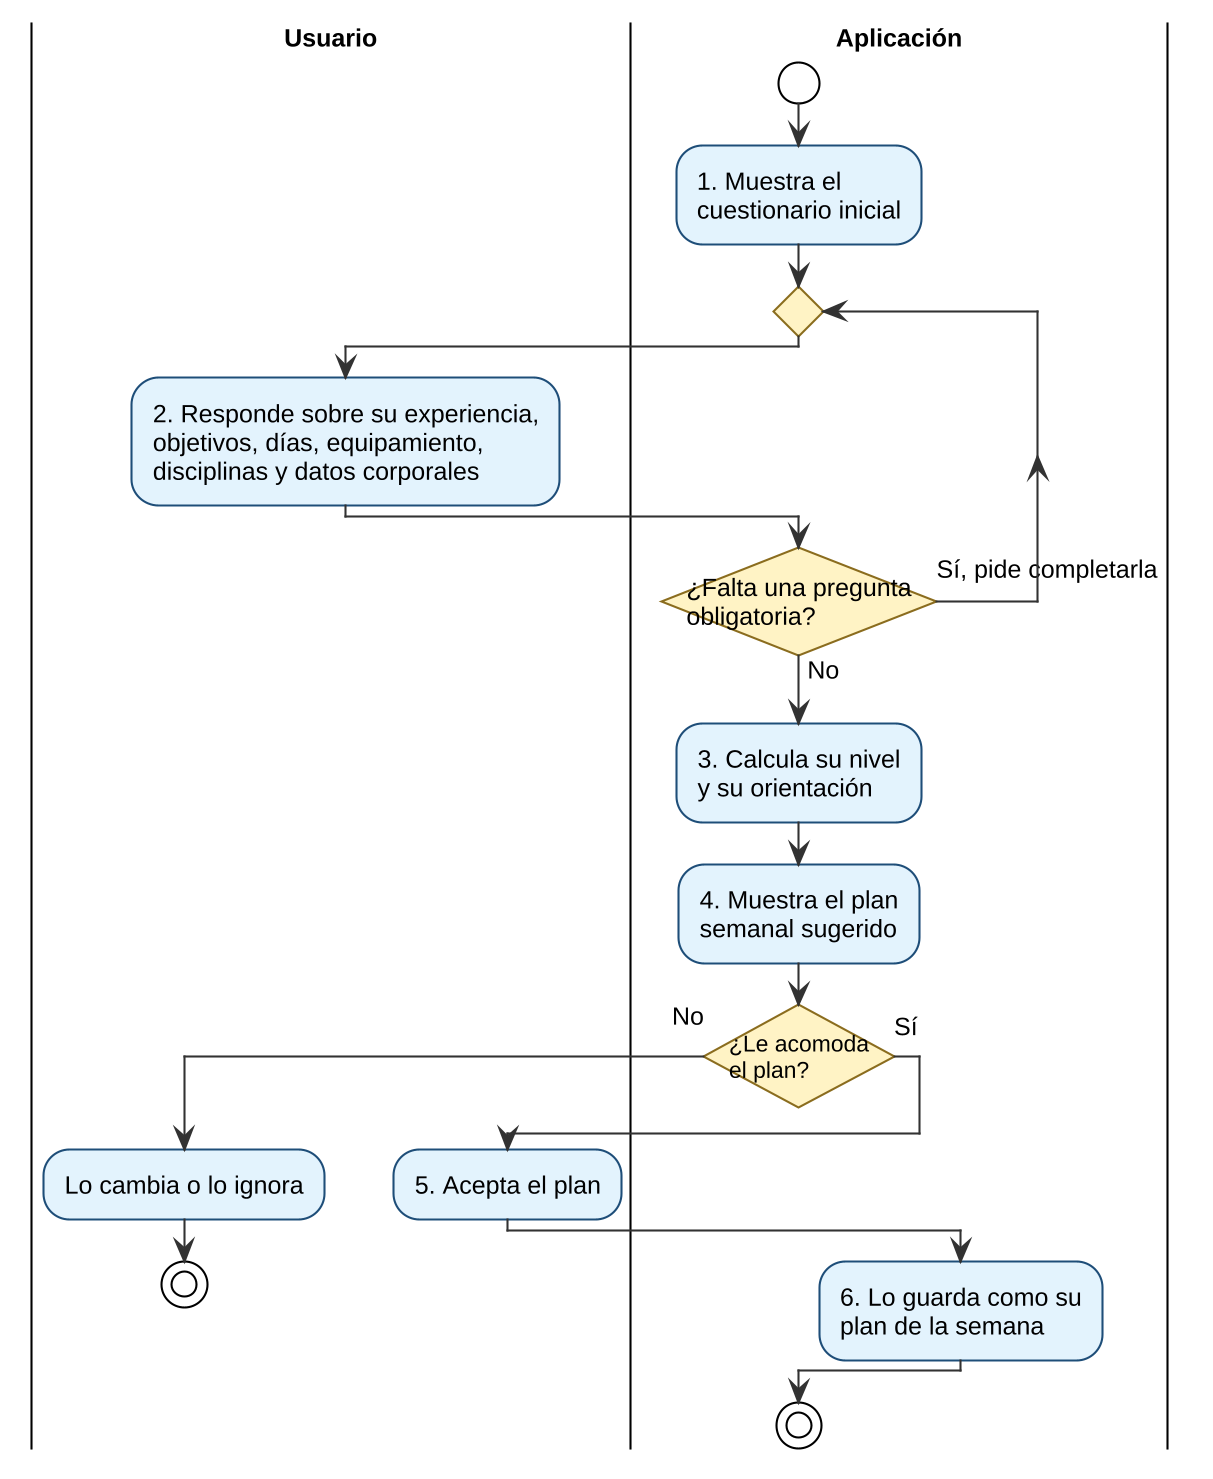
\includegraphics[width=0.78\textwidth,height=0.42\textheight,keepaspectratio]{figuras/diseno/dga_cu12.png}
    \captionof{figure}{Diagrama de Actividades -- CU-12: Completar mi perfil y recibir un plan semanal.}
    \label{fig:dga_cu12}
\end{center}

\noindent\begin{minipage}{\linewidth}
\textbf{Descripción Esencial Expandida del Caso de Uso}
\par\vspace{0.2cm}
\noindent
{\renewcommand{\arraystretch}{1.25}\setstretch{1}\small
\begin{tabular}{|>{\raggedright\arraybackslash}p{2.9cm}|>{\raggedright\arraybackslash}p{12.1cm}|}
    \hline
    \rowcolor[HTML]{EFEFEF} \textbf{Propósito} & Conocer al atleta para sugerirle un plan de entrenamiento según su nivel y sus objetivos. \\ \hline
    \textbf{Tipo} & Primario \\ \hline
    \textbf{Actores} & Atleta Básico, Atleta Híbrido \\ \hline
    \textbf{Requerimientos} & R13 \\ \hline
    \textbf{Precondiciones} & El usuario creó su cuenta y aceptó los términos de uso (CU-26). \\ \hline
    \textbf{Poscondiciones} & El perfil queda completo y el atleta tiene un plan sugerido para la semana. \\ \hline
\end{tabular}

\vspace{0.15cm}
\noindent
\begin{tabular}{|>{\raggedright\arraybackslash}p{7.5cm}|>{\raggedright\arraybackslash}p{7.5cm}|}
    \hline
    \rowcolor[HTML]{D9E1F2} \multicolumn{2}{|c|}{\textbf{Curso Normal de los Eventos}} \\ \hline
    \rowcolor[HTML]{EFEFEF} \multicolumn{1}{|c|}{\textbf{Usuario}} & \multicolumn{1}{c|}{\textbf{Respuesta del Sistema}} \\ \hline
         & 1. Muestra el cuestionario inicial. \\ \hline
        2. Responde sobre su experiencia, sus objetivos, los días que puede entrenar, su equipamiento, sus disciplinas, su edad, su sexo, su estatura y su peso. & 3. Calcula su nivel y su orientación. \\ \hline
         & 4. Muestra el plan semanal sugerido. \\ \hline
        5. Acepta el plan. & 6. Lo guarda como su plan de la semana. \\ \hline
    \rowcolor[HTML]{F2D9D9} \multicolumn{2}{|c|}{\textbf{Cursos Alternos}} \\ \hline
    \rowcolor[HTML]{EFEFEF} \multicolumn{1}{|c|}{\textbf{Usuario}} & \multicolumn{1}{c|}{\textbf{Respuesta del Sistema}} \\ \hline
        2. Si deja una pregunta obligatoria sin responder, la aplicación le pide completarla. &  \\ \hline
        5. Si no le acomoda, puede cambiar el plan o ignorarlo. La aplicación sigue funcionando igual. &  \\ \hline
\end{tabular}
}
\end{minipage}
\vspace{0.4cm}

\subsubsection{CU-13. Agregar una publicación a mis módulos}

\textbf{Diagrama de Actividades}
\begin{center}
    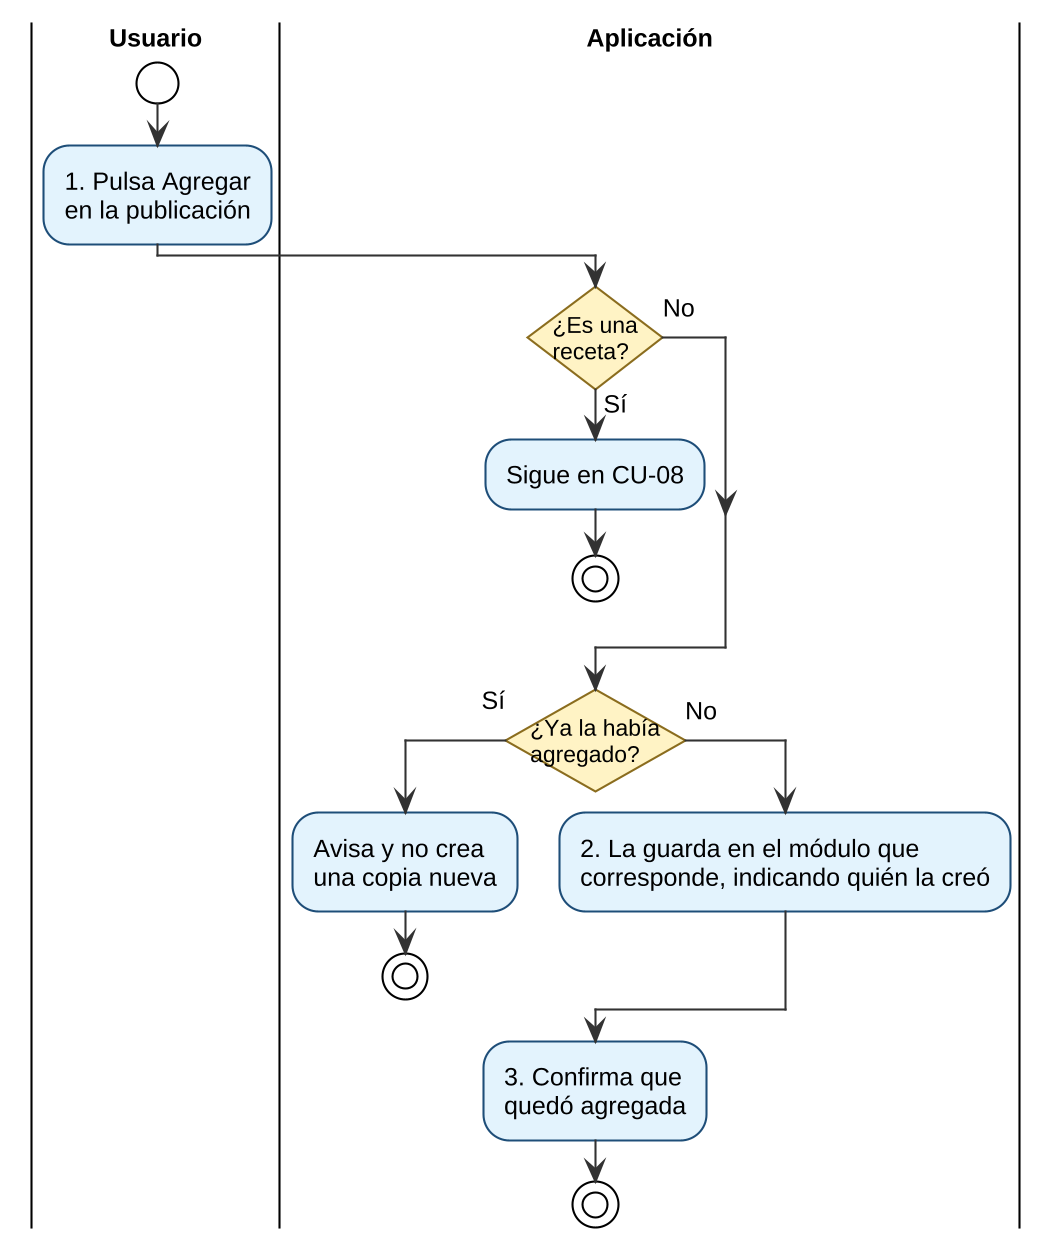
\includegraphics[width=0.78\textwidth,height=0.42\textheight,keepaspectratio]{figuras/diseno/dga_cu13.png}
    \captionof{figure}{Diagrama de Actividades -- CU-13: Agregar una publicación a mis módulos.}
    \label{fig:dga_cu13}
\end{center}

\noindent\begin{minipage}{\linewidth}
\textbf{Descripción Esencial Expandida del Caso de Uso}
\par\vspace{0.2cm}
\noindent
{\renewcommand{\arraystretch}{1.25}\setstretch{1}\small
\begin{tabular}{|>{\raggedright\arraybackslash}p{2.9cm}|>{\raggedright\arraybackslash}p{12.1cm}|}
    \hline
    \rowcolor[HTML]{EFEFEF} \textbf{Propósito} & Usar lo que publicó otra persona sin tener que copiarlo a mano. \\ \hline
    \textbf{Tipo} & Primario \\ \hline
    \textbf{Actores} & Atleta Híbrido \\ \hline
    \textbf{Requerimientos} & R12 \\ \hline
    \textbf{Precondiciones} & El usuario inició sesión y tiene el plan premium. Ve la publicación en su muro. \\ \hline
    \textbf{Poscondiciones} & El contenido queda disponible en los módulos del atleta. \\ \hline
\end{tabular}

\vspace{0.15cm}
\noindent
\begin{tabular}{|>{\raggedright\arraybackslash}p{7.5cm}|>{\raggedright\arraybackslash}p{7.5cm}|}
    \hline
    \rowcolor[HTML]{D9E1F2} \multicolumn{2}{|c|}{\textbf{Curso Normal de los Eventos}} \\ \hline
    \rowcolor[HTML]{EFEFEF} \multicolumn{1}{|c|}{\textbf{Usuario}} & \multicolumn{1}{c|}{\textbf{Respuesta del Sistema}} \\ \hline
        1. Pulsa Agregar en la publicación. & 2. La guarda en el módulo que corresponde, indicando quién la creó. Una sesión queda en sus rutinas y una ruta en su módulo de cardio. \\ \hline
         & 3. Confirma que quedó agregada. \\ \hline
    \rowcolor[HTML]{F2D9D9} \multicolumn{2}{|c|}{\textbf{Cursos Alternos}} \\ \hline
    \rowcolor[HTML]{EFEFEF} \multicolumn{1}{|c|}{\textbf{Usuario}} & \multicolumn{1}{c|}{\textbf{Respuesta del Sistema}} \\ \hline
         & 2. Si la publicación es una receta, sigue el caso de uso CU-08. \\ \hline
         & 2. Si ya la había agregado, avisa y no crea una copia nueva. \\ \hline
\end{tabular}
}
\end{minipage}
\vspace{0.4cm}

\subsubsection{CU-14. Seguir a otro usuario}

\textbf{Diagrama de Actividades}
\begin{center}
    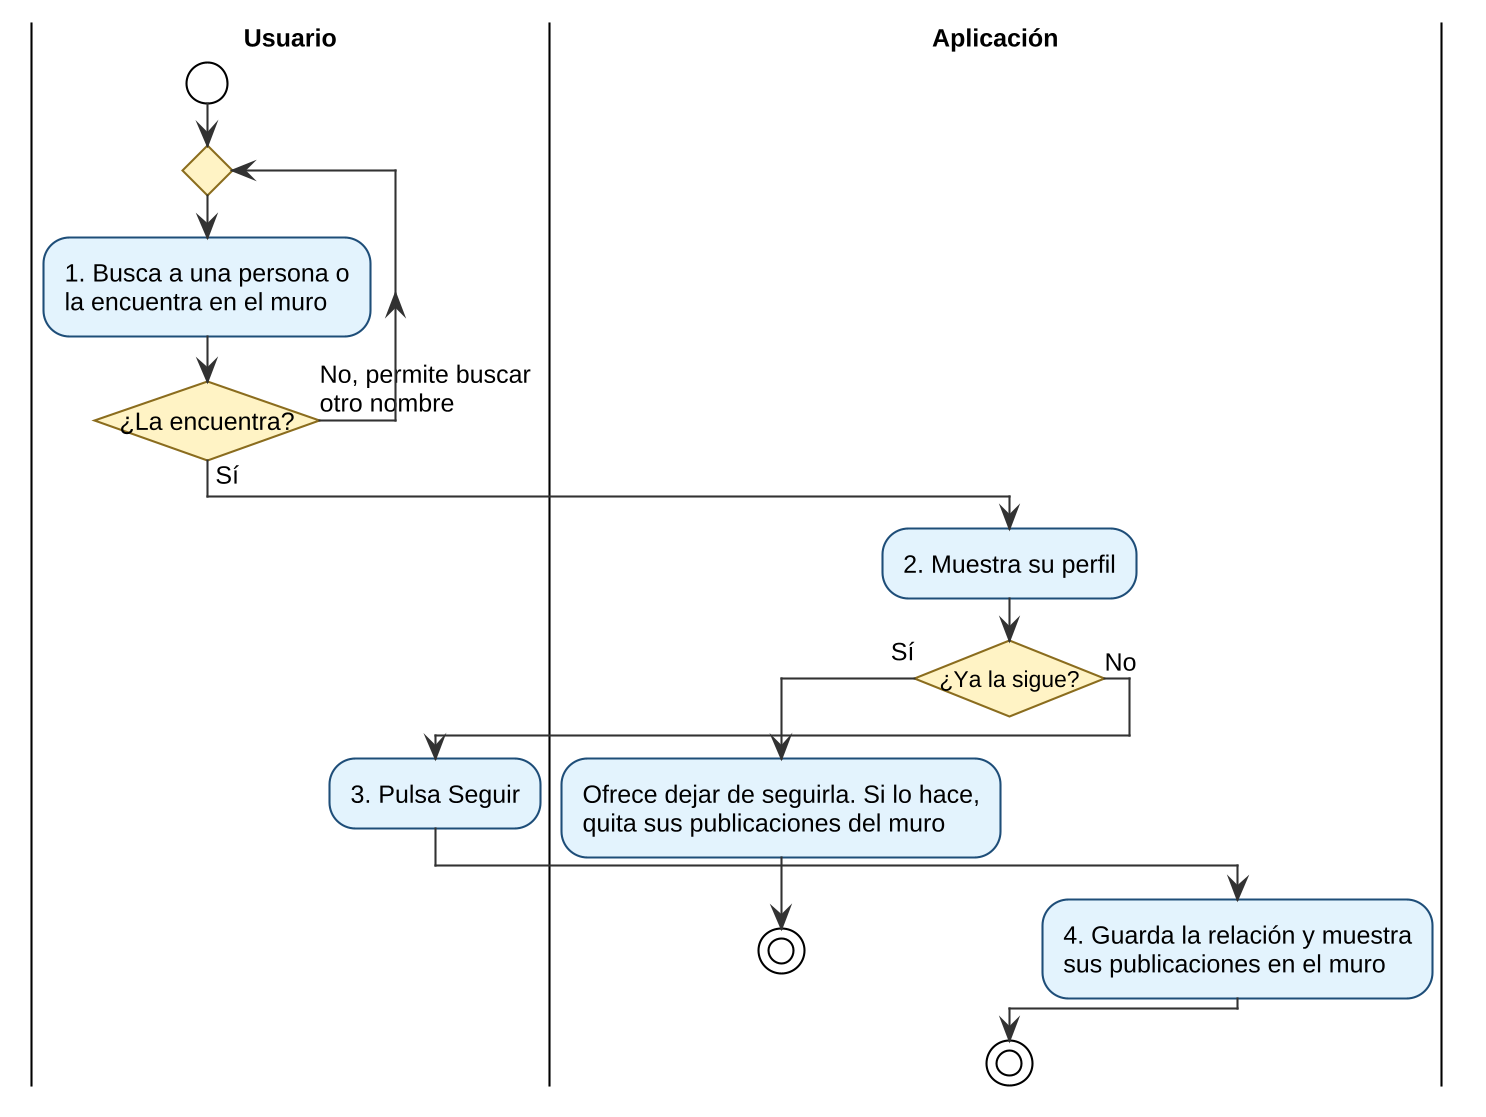
\includegraphics[width=0.78\textwidth,height=0.42\textheight,keepaspectratio]{figuras/diseno/dga_cu14.png}
    \captionof{figure}{Diagrama de Actividades -- CU-14: Seguir a otro usuario.}
    \label{fig:dga_cu14}
\end{center}

\noindent\begin{minipage}{\linewidth}
\textbf{Descripción Esencial Expandida del Caso de Uso}
\par\vspace{0.2cm}
\noindent
{\renewcommand{\arraystretch}{1.25}\setstretch{1}\small
\begin{tabular}{|>{\raggedright\arraybackslash}p{2.9cm}|>{\raggedright\arraybackslash}p{12.1cm}|}
    \hline
    \rowcolor[HTML]{EFEFEF} \textbf{Propósito} & Ver en el muro lo que publican otras personas. \\ \hline
    \textbf{Tipo} & Primario \\ \hline
    \textbf{Actores} & Atleta Híbrido \\ \hline
    \textbf{Requerimientos} & R08 \\ \hline
    \textbf{Precondiciones} & El usuario inició sesión y tiene el plan premium. \\ \hline
    \textbf{Poscondiciones} & El atleta sigue a esa persona y ve sus publicaciones. \\ \hline
\end{tabular}

\vspace{0.15cm}
\noindent
\begin{tabular}{|>{\raggedright\arraybackslash}p{7.5cm}|>{\raggedright\arraybackslash}p{7.5cm}|}
    \hline
    \rowcolor[HTML]{D9E1F2} \multicolumn{2}{|c|}{\textbf{Curso Normal de los Eventos}} \\ \hline
    \rowcolor[HTML]{EFEFEF} \multicolumn{1}{|c|}{\textbf{Usuario}} & \multicolumn{1}{c|}{\textbf{Respuesta del Sistema}} \\ \hline
        1. Busca a una persona o la encuentra en el muro. & 2. Muestra su perfil. \\ \hline
        3. Pulsa Seguir. & 4. Guarda la relación y desde ese momento muestra sus publicaciones en el muro. \\ \hline
    \rowcolor[HTML]{F2D9D9} \multicolumn{2}{|c|}{\textbf{Cursos Alternos}} \\ \hline
    \rowcolor[HTML]{EFEFEF} \multicolumn{1}{|c|}{\textbf{Usuario}} & \multicolumn{1}{c|}{\textbf{Respuesta del Sistema}} \\ \hline
         & 2. Si no encuentra a la persona, avisa y permite buscar otro nombre. \\ \hline
        3. Si ya la sigue, puede dejar de seguirla, y sus publicaciones ya no aparecen en el muro. &  \\ \hline
\end{tabular}
}
\end{minipage}
\vspace{0.4cm}

\subsubsection{CU-15. Registrar un producto con su código de barras}

\textbf{Diagrama de Actividades}
\begin{center}
    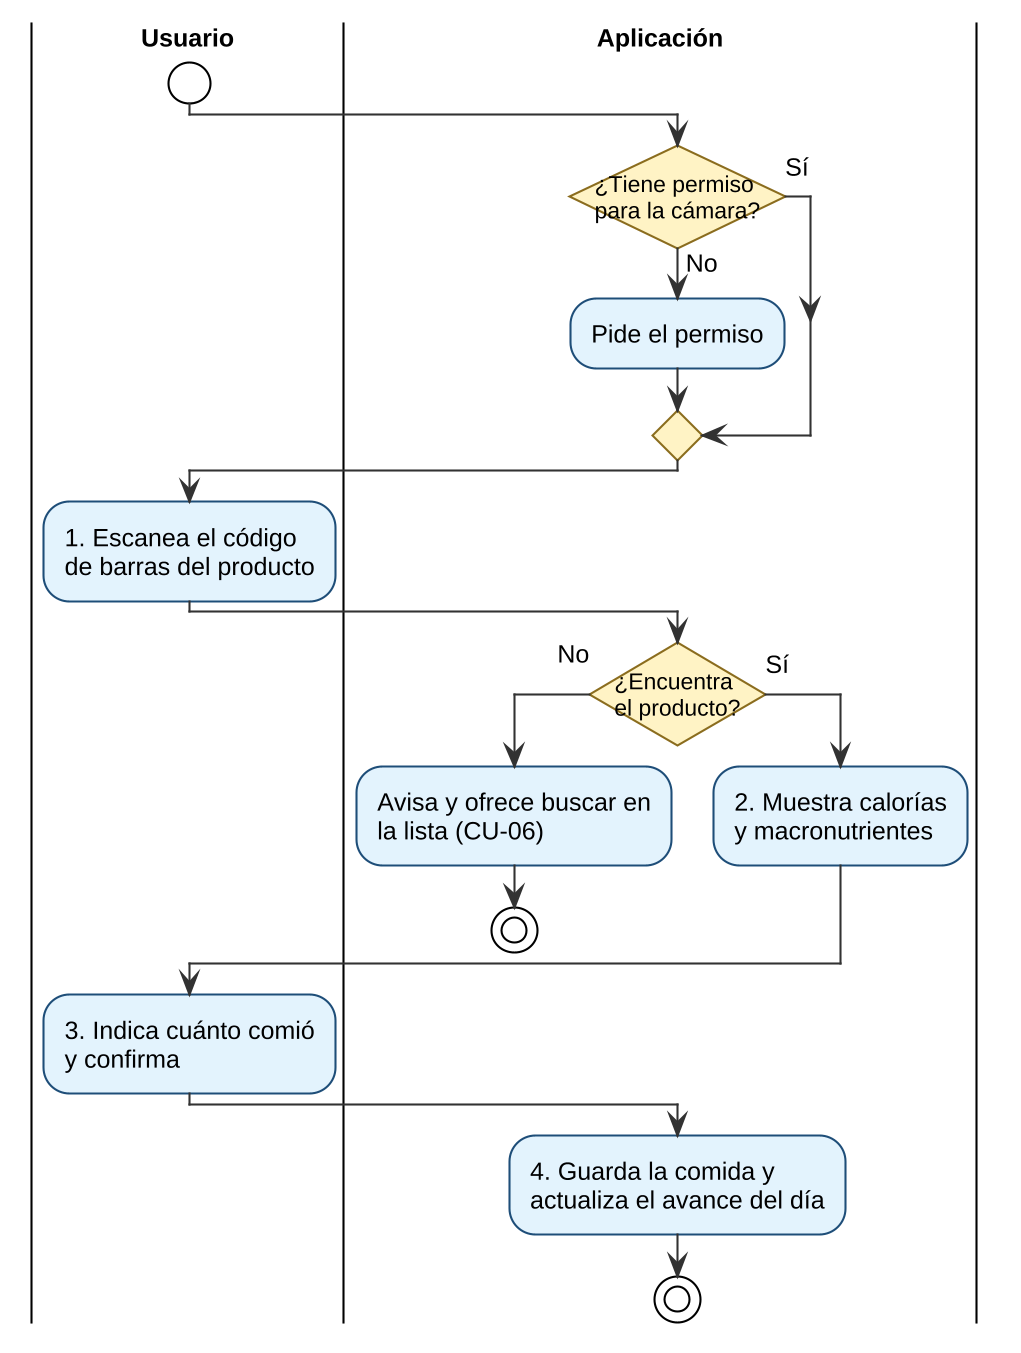
\includegraphics[width=0.78\textwidth,height=0.42\textheight,keepaspectratio]{figuras/diseno/dga_cu15.png}
    \captionof{figure}{Diagrama de Actividades -- CU-15: Registrar un producto con su código de barras.}
    \label{fig:dga_cu15}
\end{center}

\noindent\begin{minipage}{\linewidth}
\textbf{Descripción Esencial Expandida del Caso de Uso}
\par\vspace{0.2cm}
\noindent
{\renewcommand{\arraystretch}{1.25}\setstretch{1}\small
\begin{tabular}{|>{\raggedright\arraybackslash}p{2.9cm}|>{\raggedright\arraybackslash}p{12.1cm}|}
    \hline
    \rowcolor[HTML]{EFEFEF} \textbf{Propósito} & Registrar un producto envasado sin tener que buscarlo. \\ \hline
    \textbf{Tipo} & Primario \\ \hline
    \textbf{Actores} & Atleta Básico, Atleta Híbrido \\ \hline
    \textbf{Requerimientos} & R04 \\ \hline
    \textbf{Precondiciones} & El usuario inició sesión en la aplicación. \\ \hline
    \textbf{Poscondiciones} & La comida queda en el diario del día. \\ \hline
\end{tabular}

\vspace{0.15cm}
\noindent
\begin{tabular}{|>{\raggedright\arraybackslash}p{7.5cm}|>{\raggedright\arraybackslash}p{7.5cm}|}
    \hline
    \rowcolor[HTML]{D9E1F2} \multicolumn{2}{|c|}{\textbf{Curso Normal de los Eventos}} \\ \hline
    \rowcolor[HTML]{EFEFEF} \multicolumn{1}{|c|}{\textbf{Usuario}} & \multicolumn{1}{c|}{\textbf{Respuesta del Sistema}} \\ \hline
        1. Escanea con la cámara el código de barras del producto. & 2. Muestra el producto con sus calorías y sus macronutrientes. \\ \hline
        3. Indica cuánto comió y confirma. & 4. Guarda la comida en el diario y actualiza el avance del día. \\ \hline
    \rowcolor[HTML]{F2D9D9} \multicolumn{2}{|c|}{\textbf{Cursos Alternos}} \\ \hline
    \rowcolor[HTML]{EFEFEF} \multicolumn{1}{|c|}{\textbf{Usuario}} & \multicolumn{1}{c|}{\textbf{Respuesta del Sistema}} \\ \hline
        1. Si no ha dado permiso para usar la cámara, la aplicación se lo pide. &  \\ \hline
         & 2. Si no encuentra el producto, avisa y ofrece buscarlo en la lista de alimentos (CU-06). \\ \hline
\end{tabular}
}
\end{minipage}
\vspace{0.4cm}

\subsubsection{CU-16. Contar mi comida con mis palabras}

\textbf{Diagrama de Actividades}
\begin{center}
    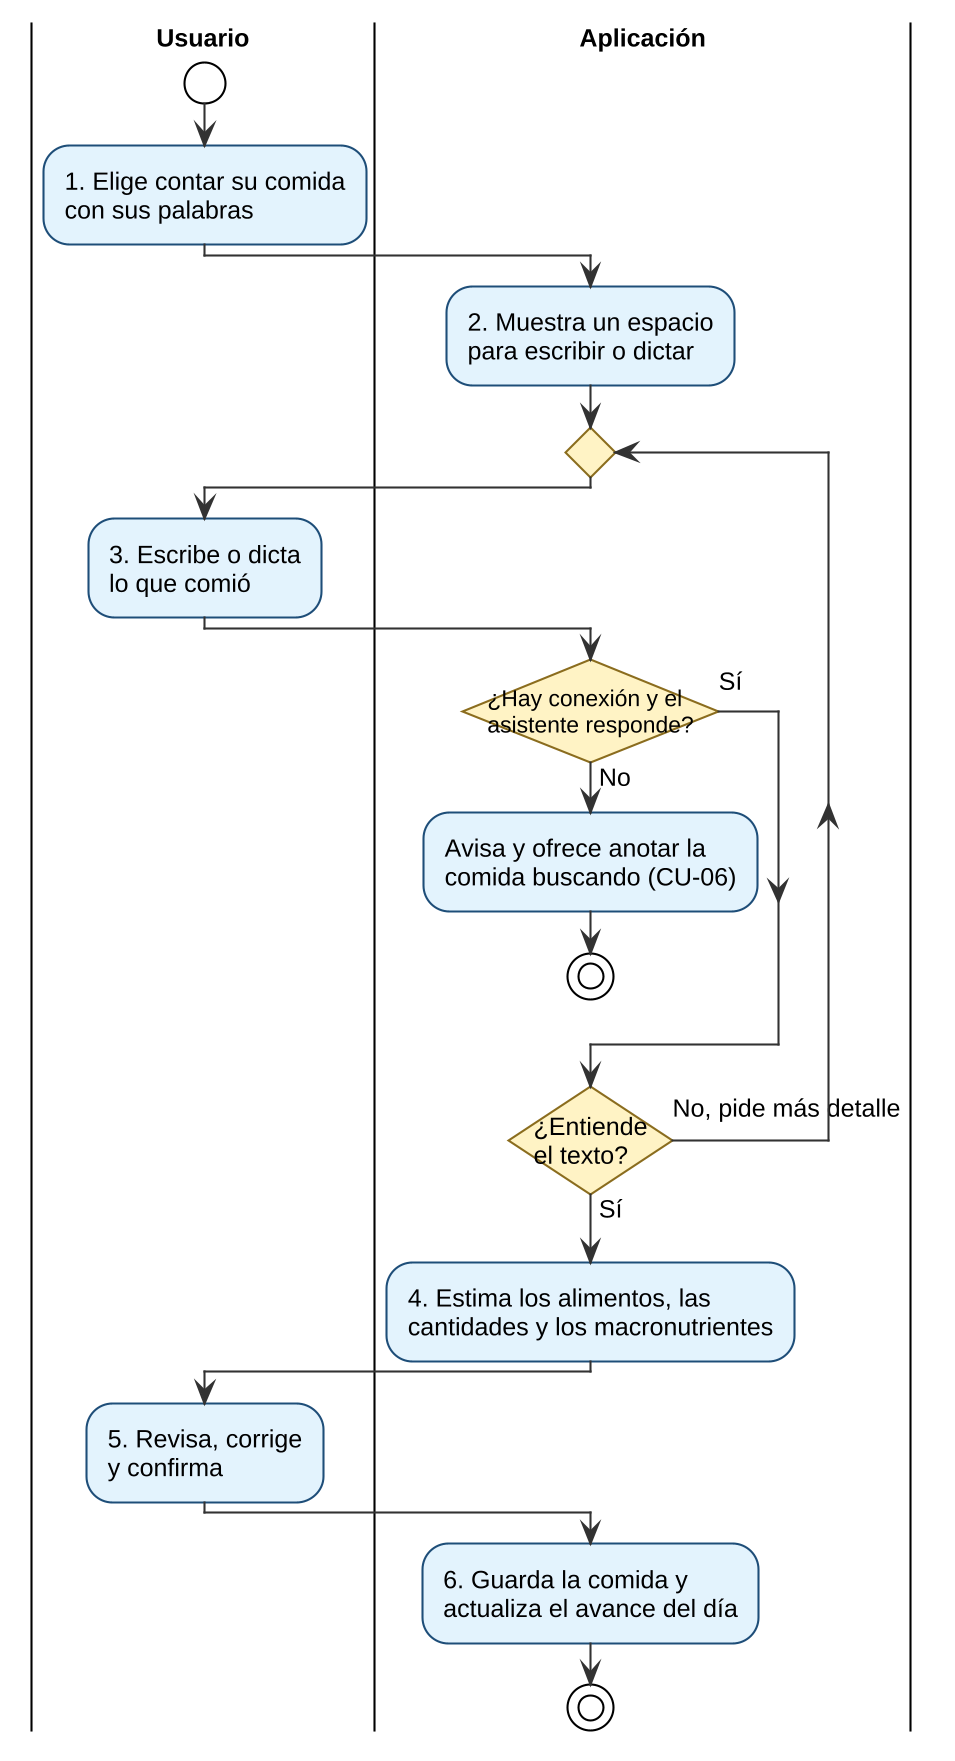
\includegraphics[width=0.78\textwidth,height=0.42\textheight,keepaspectratio]{figuras/diseno/dga_cu16.png}
    \captionof{figure}{Diagrama de Actividades -- CU-16: Contar mi comida con mis palabras.}
    \label{fig:dga_cu16}
\end{center}

\noindent\begin{minipage}{\linewidth}
\textbf{Descripción Esencial Expandida del Caso de Uso}
\par\vspace{0.2cm}
\noindent
{\renewcommand{\arraystretch}{1.25}\setstretch{1}\small
\begin{tabular}{|>{\raggedright\arraybackslash}p{2.9cm}|>{\raggedright\arraybackslash}p{12.1cm}|}
    \hline
    \rowcolor[HTML]{EFEFEF} \textbf{Propósito} & Registrar una comida escribiendo o dictando lo que se comió. \\ \hline
    \textbf{Tipo} & Primario \\ \hline
    \textbf{Actores} & Atleta Híbrido, Asistente de inteligencia artificial \\ \hline
    \textbf{Requerimientos} & R04 \\ \hline
    \textbf{Precondiciones} & El usuario inició sesión y tiene el plan premium. Tiene conexión a Internet. \\ \hline
    \textbf{Poscondiciones} & La comida confirmada queda en el diario del día. \\ \hline
\end{tabular}

\vspace{0.15cm}
\noindent
\begin{tabular}{|>{\raggedright\arraybackslash}p{7.5cm}|>{\raggedright\arraybackslash}p{7.5cm}|}
    \hline
    \rowcolor[HTML]{D9E1F2} \multicolumn{2}{|c|}{\textbf{Curso Normal de los Eventos}} \\ \hline
    \rowcolor[HTML]{EFEFEF} \multicolumn{1}{|c|}{\textbf{Usuario}} & \multicolumn{1}{c|}{\textbf{Respuesta del Sistema}} \\ \hline
        1. Elige contar su comida con sus palabras. & 2. Muestra un espacio para escribir o dictar. \\ \hline
        3. Escribe o dicta lo que comió, por ejemplo ``un plato de arroz con pollo y una ensalada''. & 4. Estima con ayuda del asistente de IA los alimentos, las cantidades y los macronutrientes. \\ \hline
        5. Revisa la estimación, corrige lo que haga falta y confirma. & 6. Guarda la comida en el diario y actualiza el avance del día. \\ \hline
    \rowcolor[HTML]{F2D9D9} \multicolumn{2}{|c|}{\textbf{Cursos Alternos}} \\ \hline
    \rowcolor[HTML]{EFEFEF} \multicolumn{1}{|c|}{\textbf{Usuario}} & \multicolumn{1}{c|}{\textbf{Respuesta del Sistema}} \\ \hline
         & 4. Si no logra entender el texto, pide al atleta que dé más detalle. \\ \hline
         & 4. Si no hay conexión o el asistente no responde, avisa y ofrece anotar la comida buscando los alimentos (CU-06). \\ \hline
\end{tabular}
}
\end{minipage}
\vspace{0.4cm}

\subsubsection{CU-17. Registrar una sesión de cardio sin reloj}

\textbf{Diagrama de Actividades}
\begin{center}
    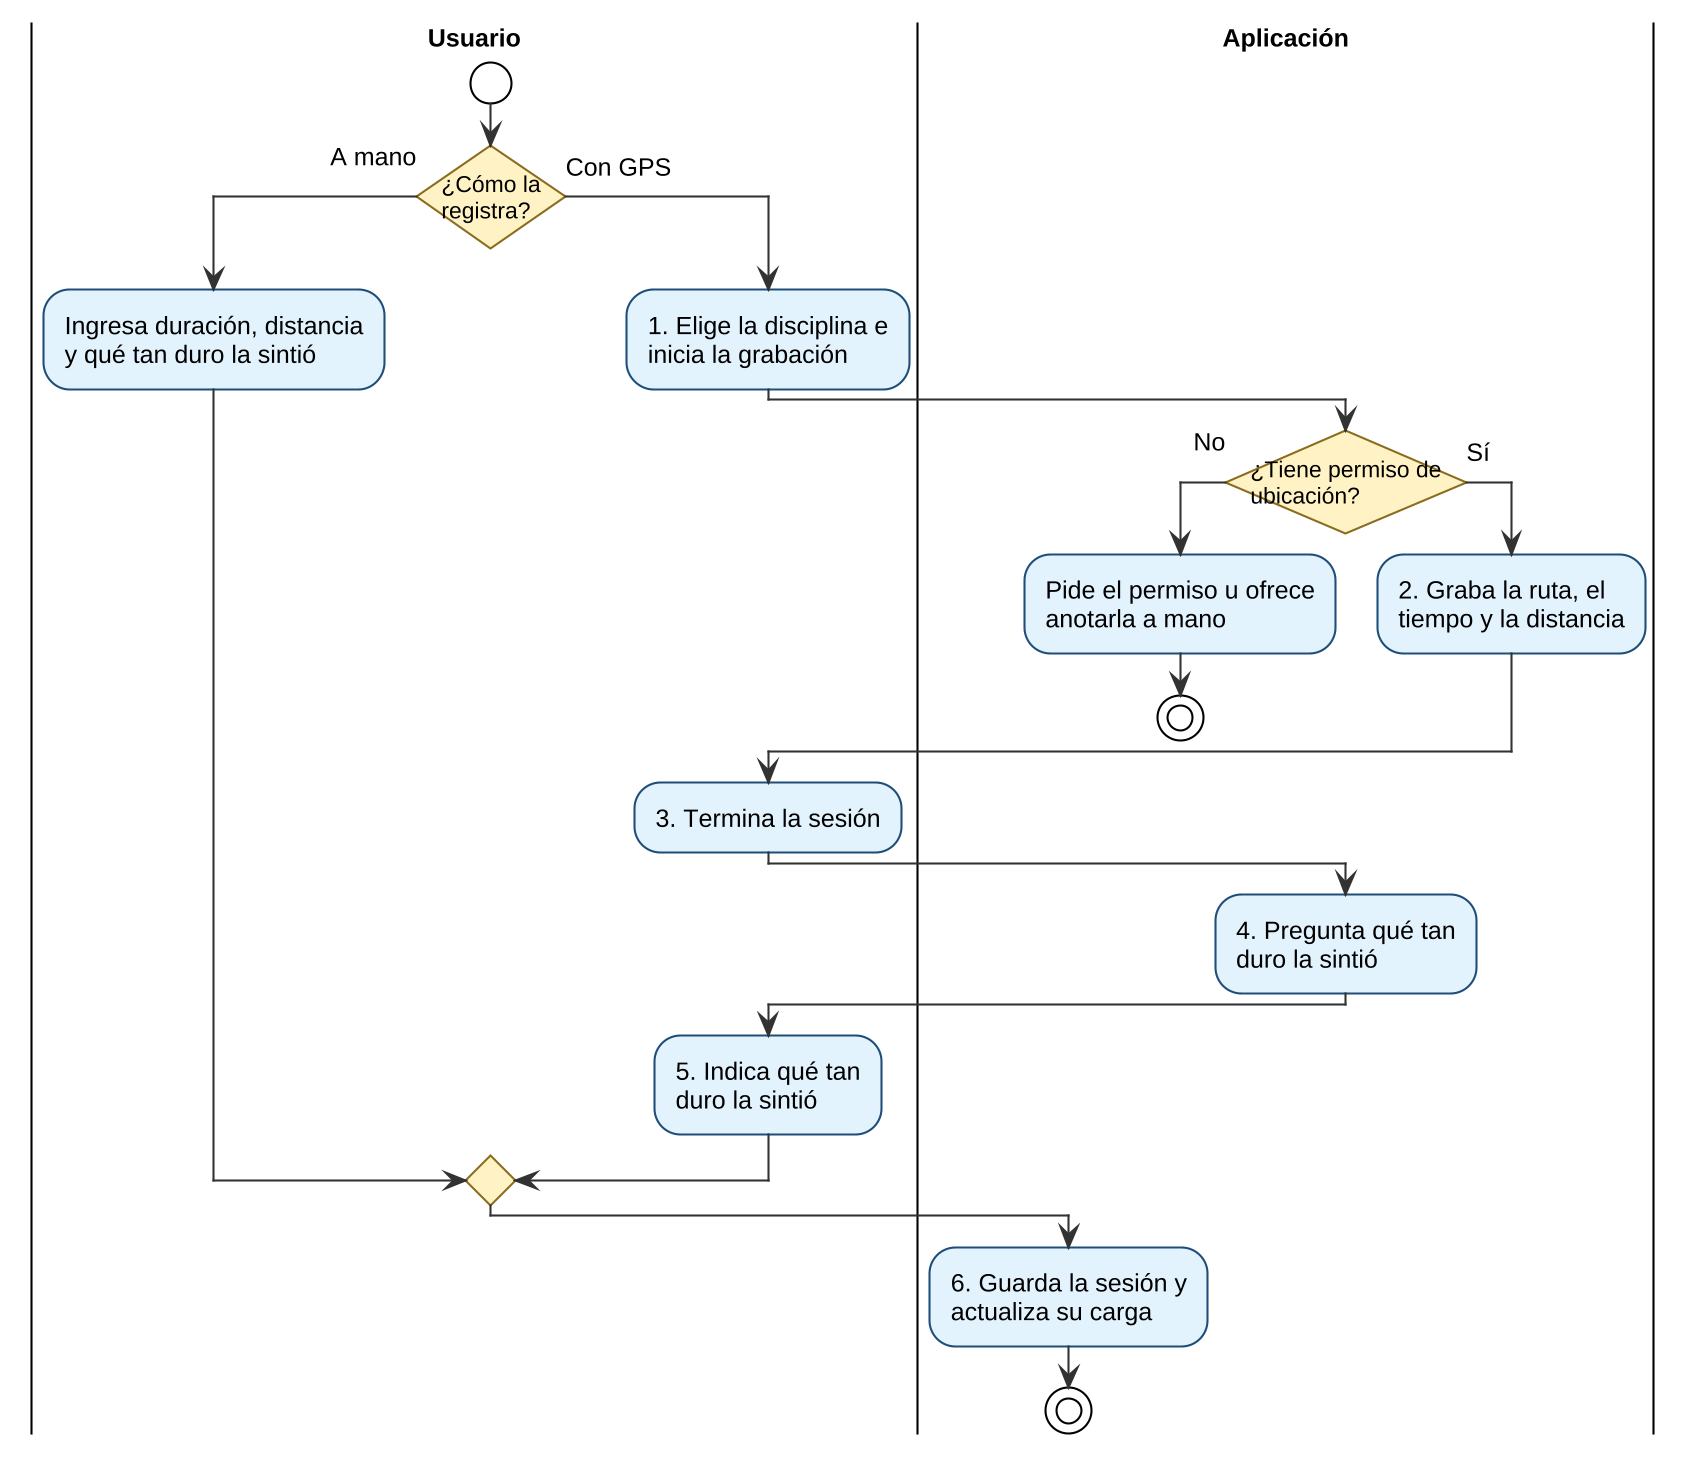
\includegraphics[width=0.78\textwidth,height=0.42\textheight,keepaspectratio]{figuras/diseno/dga_cu17.png}
    \captionof{figure}{Diagrama de Actividades -- CU-17: Registrar una sesión de cardio sin reloj.}
    \label{fig:dga_cu17}
\end{center}

\noindent\begin{minipage}{\linewidth}
\textbf{Descripción Esencial Expandida del Caso de Uso}
\par\vspace{0.2cm}
\noindent
{\renewcommand{\arraystretch}{1.25}\setstretch{1}\small
\begin{tabular}{|>{\raggedright\arraybackslash}p{2.9cm}|>{\raggedright\arraybackslash}p{12.1cm}|}
    \hline
    \rowcolor[HTML]{EFEFEF} \textbf{Propósito} & Registrar una salida de ciclismo, running o trekking usando solo el teléfono. \\ \hline
    \textbf{Tipo} & Primario \\ \hline
    \textbf{Actores} & Atleta Básico, Atleta Híbrido \\ \hline
    \textbf{Requerimientos} & R02 \\ \hline
    \textbf{Precondiciones} & El usuario inició sesión en la aplicación. \\ \hline
    \textbf{Poscondiciones} & La sesión queda en el historial del atleta y su carga queda actualizada. \\ \hline
\end{tabular}

\vspace{0.15cm}
\noindent
\begin{tabular}{|>{\raggedright\arraybackslash}p{7.5cm}|>{\raggedright\arraybackslash}p{7.5cm}|}
    \hline
    \rowcolor[HTML]{D9E1F2} \multicolumn{2}{|c|}{\textbf{Curso Normal de los Eventos}} \\ \hline
    \rowcolor[HTML]{EFEFEF} \multicolumn{1}{|c|}{\textbf{Usuario}} & \multicolumn{1}{c|}{\textbf{Respuesta del Sistema}} \\ \hline
        1. Elige la disciplina e inicia la grabación. & 2. Graba la ruta, el tiempo y la distancia con el GPS del teléfono. \\ \hline
        3. Termina la sesión. & 4. Pregunta qué tan duro la sintió. \\ \hline
        5. Indica qué tan duro la sintió. & 6. Guarda la sesión y actualiza su carga. \\ \hline
    \rowcolor[HTML]{F2D9D9} \multicolumn{2}{|c|}{\textbf{Cursos Alternos}} \\ \hline
    \rowcolor[HTML]{EFEFEF} \multicolumn{1}{|c|}{\textbf{Usuario}} & \multicolumn{1}{c|}{\textbf{Respuesta del Sistema}} \\ \hline
        1. Si prefiere anotarla a mano, ingresa la duración, la distancia y qué tan duro la sintió, y sigue en el paso 6. &  \\ \hline
         & 2. Si no tiene permiso para usar la ubicación, lo pide. Sin permiso, ofrece anotar la sesión a mano. \\ \hline
\end{tabular}
}
\end{minipage}
\vspace{0.4cm}

\subsubsection{CU-18. Ver mis metas de alimentación del día}

\textbf{Diagrama de Actividades}
\begin{center}
    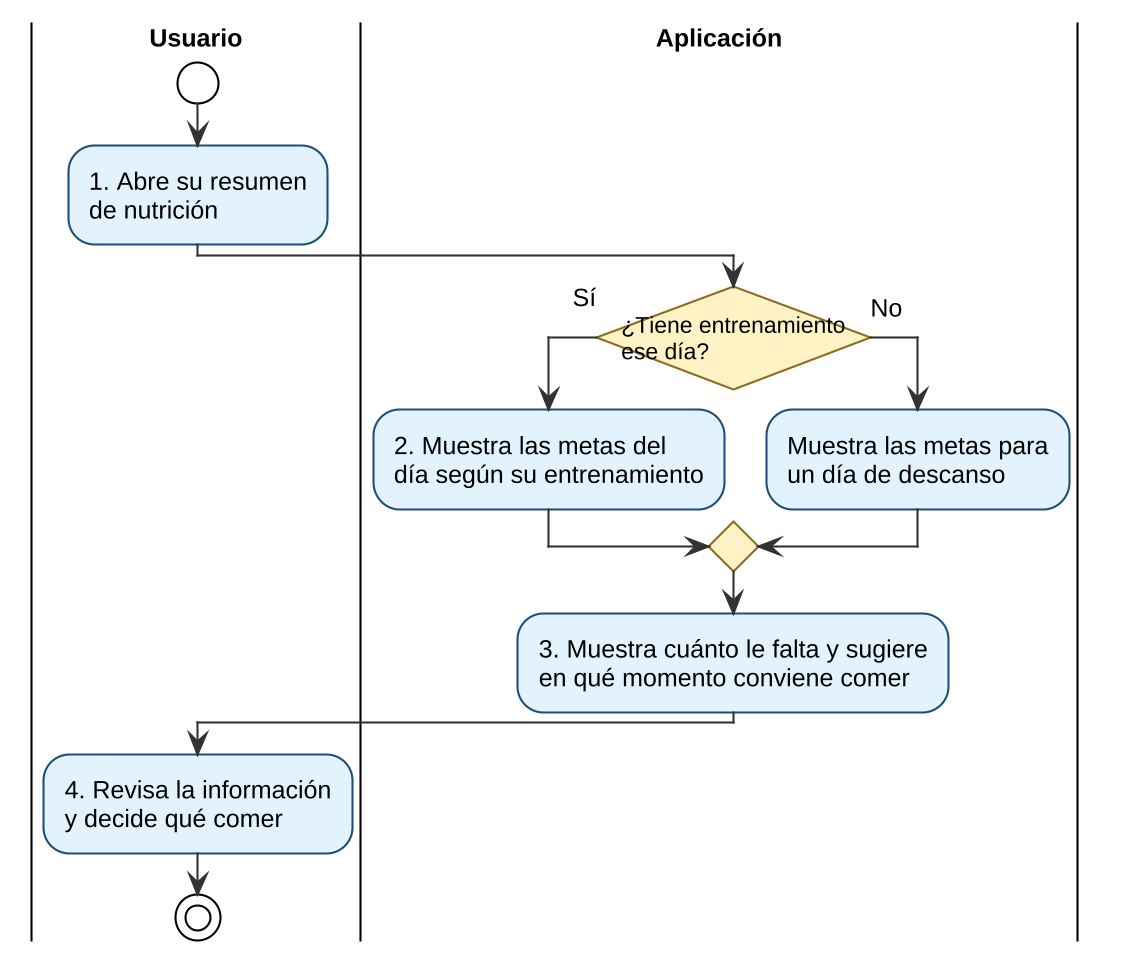
\includegraphics[width=0.78\textwidth,height=0.42\textheight,keepaspectratio]{figuras/diseno/dga_cu18.png}
    \captionof{figure}{Diagrama de Actividades -- CU-18: Ver mis metas de alimentación del día.}
    \label{fig:dga_cu18}
\end{center}

\noindent\begin{minipage}{\linewidth}
\textbf{Descripción Esencial Expandida del Caso de Uso}
\par\vspace{0.2cm}
\noindent
{\renewcommand{\arraystretch}{1.25}\setstretch{1}\small
\begin{tabular}{|>{\raggedright\arraybackslash}p{2.9cm}|>{\raggedright\arraybackslash}p{12.1cm}|}
    \hline
    \rowcolor[HTML]{EFEFEF} \textbf{Propósito} & Mostrar cuánto le conviene comer al atleta según lo que entrenó o tiene planificado. \\ \hline
    \textbf{Tipo} & Primario \\ \hline
    \textbf{Actores} & Atleta Híbrido \\ \hline
    \textbf{Requerimientos} & R05 \\ \hline
    \textbf{Precondiciones} & El usuario inició sesión y tiene el plan premium. Completó su perfil. \\ \hline
    \textbf{Poscondiciones} & El atleta conoce sus metas del día. Son sugerencias y no una dieta. \\ \hline
\end{tabular}

\vspace{0.15cm}
\noindent
\begin{tabular}{|>{\raggedright\arraybackslash}p{7.5cm}|>{\raggedright\arraybackslash}p{7.5cm}|}
    \hline
    \rowcolor[HTML]{D9E1F2} \multicolumn{2}{|c|}{\textbf{Curso Normal de los Eventos}} \\ \hline
    \rowcolor[HTML]{EFEFEF} \multicolumn{1}{|c|}{\textbf{Usuario}} & \multicolumn{1}{c|}{\textbf{Respuesta del Sistema}} \\ \hline
        1. Abre su resumen de nutrición. & 2. Muestra las metas de calorías y macronutrientes del día, según su entrenamiento. \\ \hline
         & 3. Muestra cuánto le falta y sugiere en qué momento conviene comer. \\ \hline
        4. Revisa la información y decide qué comer. &  \\ \hline
    \rowcolor[HTML]{F2D9D9} \multicolumn{2}{|c|}{\textbf{Cursos Alternos}} \\ \hline
    \rowcolor[HTML]{EFEFEF} \multicolumn{1}{|c|}{\textbf{Usuario}} & \multicolumn{1}{c|}{\textbf{Respuesta del Sistema}} \\ \hline
         & 2. Si ese día no tiene entrenamiento, muestra las metas para un día de descanso. \\ \hline
\end{tabular}
}
\end{minipage}
\vspace{0.4cm}

\subsubsection{CU-19. Revisar mi progreso}

\textbf{Diagrama de Actividades}
\begin{center}
    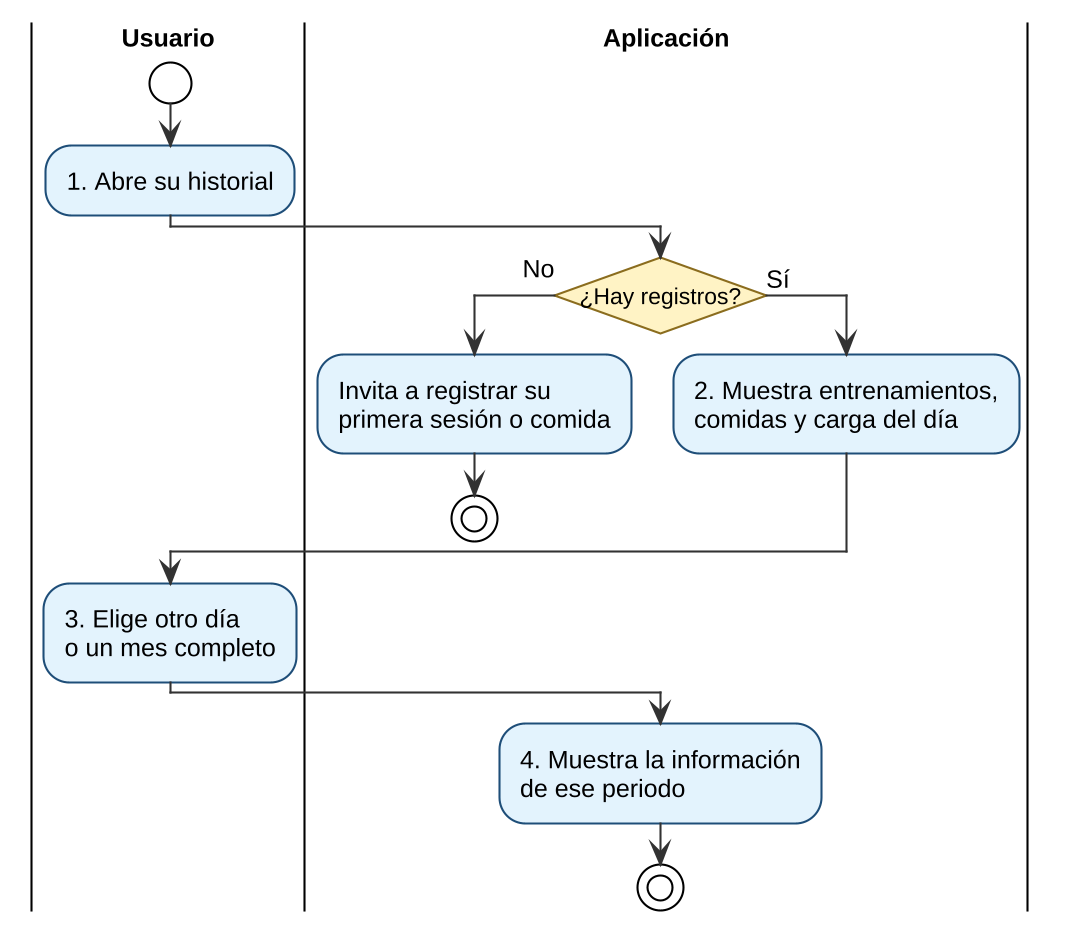
\includegraphics[width=0.78\textwidth,height=0.42\textheight,keepaspectratio]{figuras/diseno/dga_cu19.png}
    \captionof{figure}{Diagrama de Actividades -- CU-19: Revisar mi progreso.}
    \label{fig:dga_cu19}
\end{center}

\noindent\begin{minipage}{\linewidth}
\textbf{Descripción Esencial Expandida del Caso de Uso}
\par\vspace{0.2cm}
\noindent
{\renewcommand{\arraystretch}{1.25}\setstretch{1}\small
\begin{tabular}{|>{\raggedright\arraybackslash}p{2.9cm}|>{\raggedright\arraybackslash}p{12.1cm}|}
    \hline
    \rowcolor[HTML]{EFEFEF} \textbf{Propósito} & Ver en un solo lugar los entrenamientos, las comidas y la carga acumulada. \\ \hline
    \textbf{Tipo} & Primario \\ \hline
    \textbf{Actores} & Atleta Básico, Atleta Híbrido \\ \hline
    \textbf{Requerimientos} & R06 \\ \hline
    \textbf{Precondiciones} & El usuario inició sesión en la aplicación. \\ \hline
    \textbf{Poscondiciones} & El atleta ve su progreso. No se modifica ningún dato. \\ \hline
\end{tabular}

\vspace{0.15cm}
\noindent
\begin{tabular}{|>{\raggedright\arraybackslash}p{7.5cm}|>{\raggedright\arraybackslash}p{7.5cm}|}
    \hline
    \rowcolor[HTML]{D9E1F2} \multicolumn{2}{|c|}{\textbf{Curso Normal de los Eventos}} \\ \hline
    \rowcolor[HTML]{EFEFEF} \multicolumn{1}{|c|}{\textbf{Usuario}} & \multicolumn{1}{c|}{\textbf{Respuesta del Sistema}} \\ \hline
        1. Abre su historial. & 2. Muestra los entrenamientos, las comidas y la carga del día. \\ \hline
        3. Elige otro día o un mes completo. & 4. Muestra la información de ese periodo. \\ \hline
    \rowcolor[HTML]{F2D9D9} \multicolumn{2}{|c|}{\textbf{Cursos Alternos}} \\ \hline
    \rowcolor[HTML]{EFEFEF} \multicolumn{1}{|c|}{\textbf{Usuario}} & \multicolumn{1}{c|}{\textbf{Respuesta del Sistema}} \\ \hline
         & 2. Si todavía no hay registros, invita al atleta a registrar su primera sesión o comida. \\ \hline
\end{tabular}
}
\end{minipage}
\vspace{0.4cm}

\subsubsection{CU-20. Anotar cómo me sentí}

\textbf{Diagrama de Actividades}
\begin{center}
    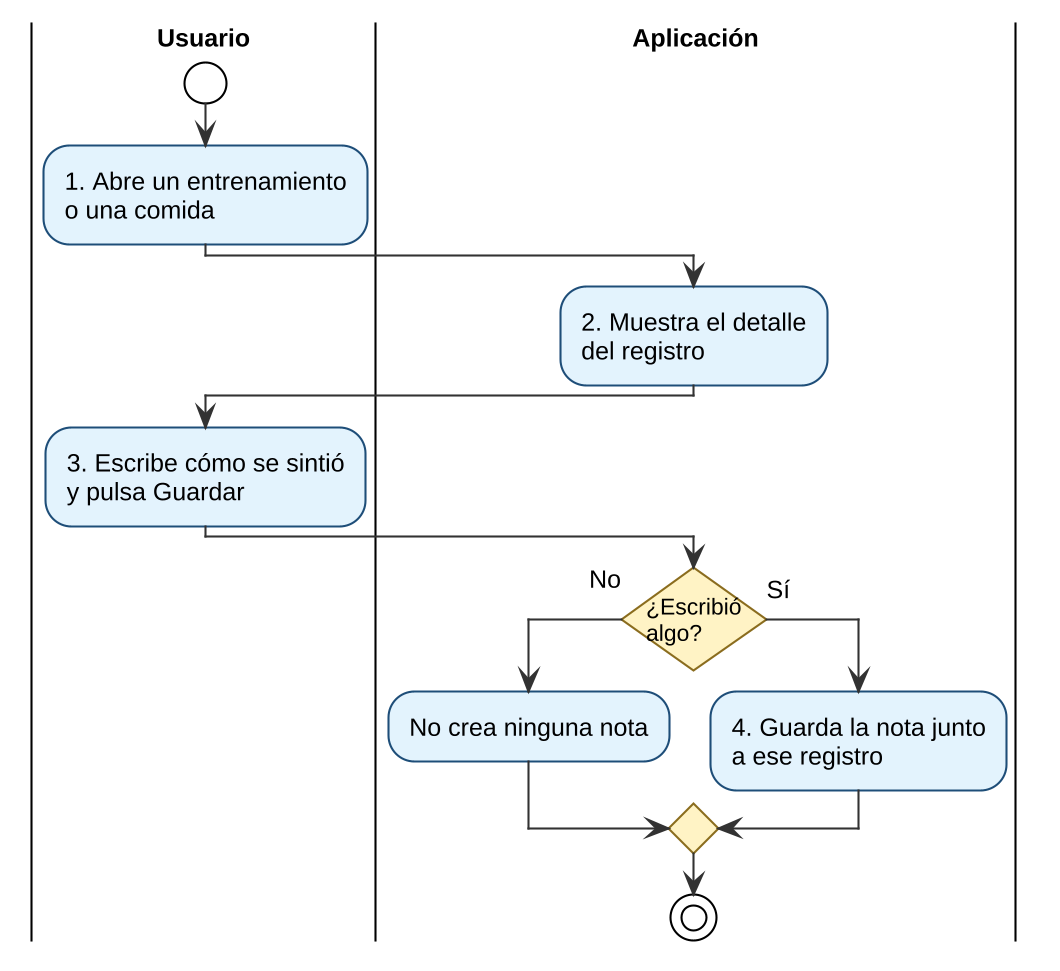
\includegraphics[width=0.78\textwidth,height=0.42\textheight,keepaspectratio]{figuras/diseno/dga_cu20.png}
    \captionof{figure}{Diagrama de Actividades -- CU-20: Anotar cómo me sentí.}
    \label{fig:dga_cu20}
\end{center}

\noindent\begin{minipage}{\linewidth}
\textbf{Descripción Esencial Expandida del Caso de Uso}
\par\vspace{0.2cm}
\noindent
{\renewcommand{\arraystretch}{1.25}\setstretch{1}\small
\begin{tabular}{|>{\raggedright\arraybackslash}p{2.9cm}|>{\raggedright\arraybackslash}p{12.1cm}|}
    \hline
    \rowcolor[HTML]{EFEFEF} \textbf{Propósito} & Guardar cómo se sintió el atleta física y digestivamente, para revisarlo después. \\ \hline
    \textbf{Tipo} & Primario \\ \hline
    \textbf{Actores} & Atleta Básico, Atleta Híbrido \\ \hline
    \textbf{Requerimientos} & R07 \\ \hline
    \textbf{Precondiciones} & El usuario inició sesión en la aplicación. Tiene un entrenamiento o una comida registrada. \\ \hline
    \textbf{Poscondiciones} & La nota queda junto al entrenamiento o la comida. \\ \hline
\end{tabular}

\vspace{0.15cm}
\noindent
\begin{tabular}{|>{\raggedright\arraybackslash}p{7.5cm}|>{\raggedright\arraybackslash}p{7.5cm}|}
    \hline
    \rowcolor[HTML]{D9E1F2} \multicolumn{2}{|c|}{\textbf{Curso Normal de los Eventos}} \\ \hline
    \rowcolor[HTML]{EFEFEF} \multicolumn{1}{|c|}{\textbf{Usuario}} & \multicolumn{1}{c|}{\textbf{Respuesta del Sistema}} \\ \hline
        1. Abre un entrenamiento o una comida. & 2. Muestra el detalle del registro. \\ \hline
        3. Escribe cómo se sintió y pulsa Guardar. & 4. Guarda la nota junto a ese registro. \\ \hline
    \rowcolor[HTML]{F2D9D9} \multicolumn{2}{|c|}{\textbf{Cursos Alternos}} \\ \hline
    \rowcolor[HTML]{EFEFEF} \multicolumn{1}{|c|}{\textbf{Usuario}} & \multicolumn{1}{c|}{\textbf{Respuesta del Sistema}} \\ \hline
        3. Si pulsa Guardar sin escribir nada, la aplicación no crea ninguna nota. &  \\ \hline
\end{tabular}
}
\end{minipage}
\vspace{0.4cm}

\subsubsection{CU-21. Controlar mis datos personales}

\textbf{Diagrama de Actividades}
\begin{center}
    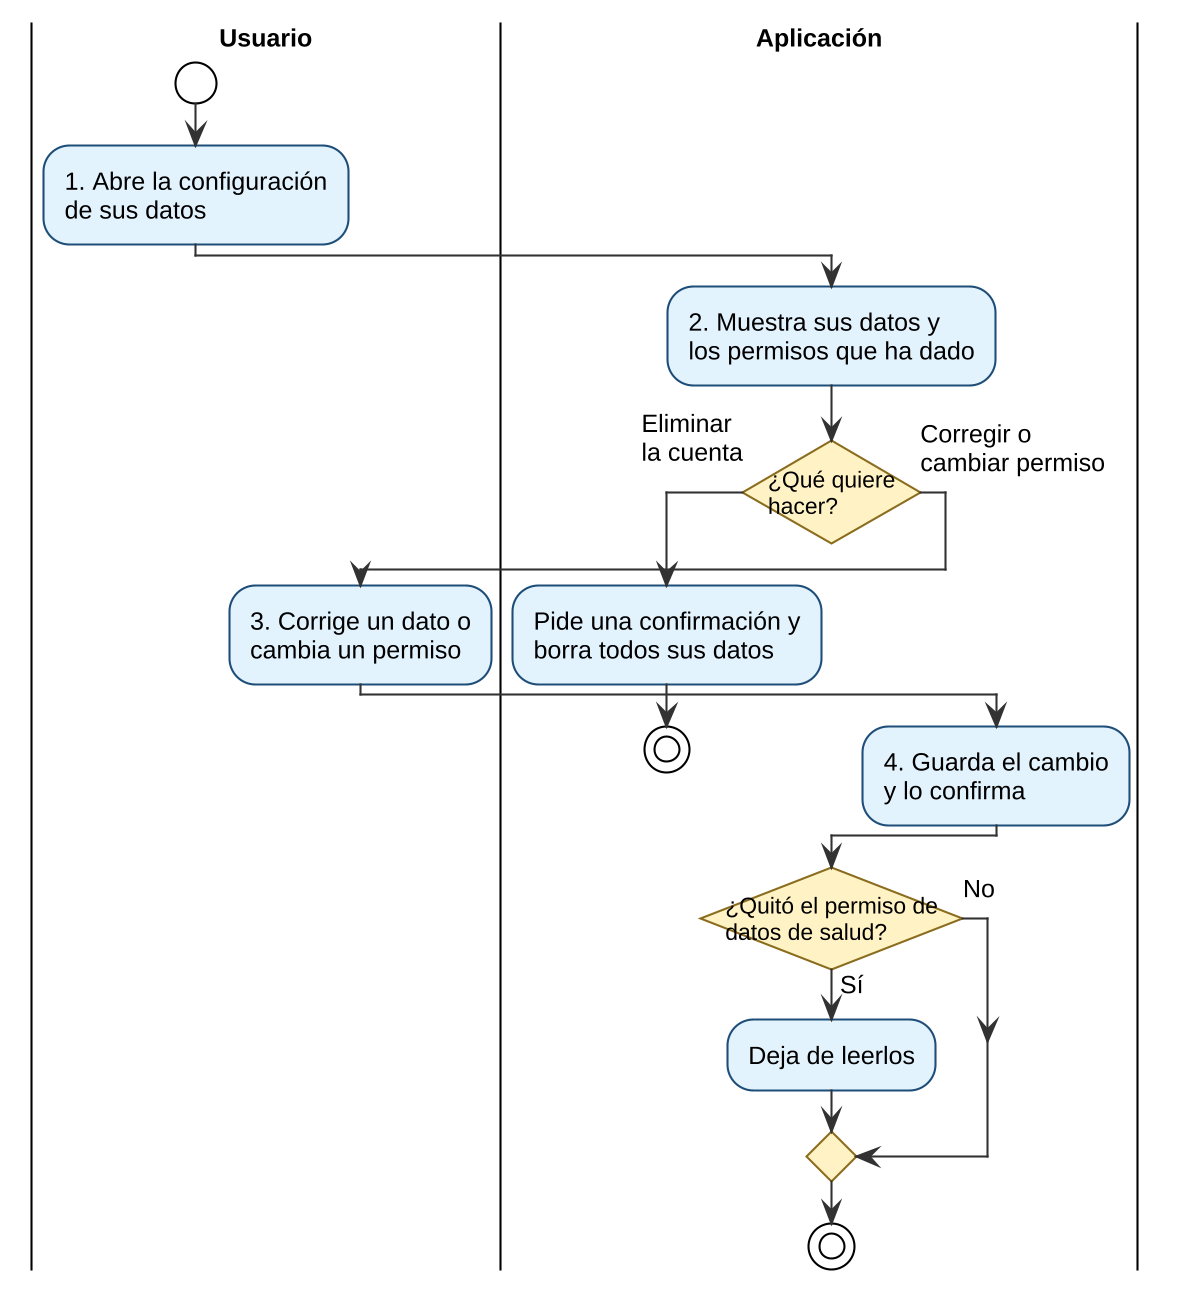
\includegraphics[width=0.78\textwidth,height=0.42\textheight,keepaspectratio]{figuras/diseno/dga_cu21.png}
    \captionof{figure}{Diagrama de Actividades -- CU-21: Controlar mis datos personales.}
    \label{fig:dga_cu21}
\end{center}

\noindent\begin{minipage}{\linewidth}
\textbf{Descripción Esencial Expandida del Caso de Uso}
\par\vspace{0.2cm}
\noindent
{\renewcommand{\arraystretch}{1.25}\setstretch{1}\small
\begin{tabular}{|>{\raggedright\arraybackslash}p{2.9cm}|>{\raggedright\arraybackslash}p{12.1cm}|}
    \hline
    \rowcolor[HTML]{EFEFEF} \textbf{Propósito} & Dar al atleta el control sobre sus datos, como pide la Ley N° 19.628. \\ \hline
    \textbf{Tipo} & Primario \\ \hline
    \textbf{Actores} & Atleta Básico, Atleta Híbrido, App de salud del teléfono \\ \hline
    \textbf{Requerimientos} & R09 \\ \hline
    \textbf{Precondiciones} & El usuario inició sesión en la aplicación. \\ \hline
    \textbf{Poscondiciones} & Los datos y los permisos quedan como el atleta los dejó. \\ \hline
\end{tabular}

\vspace{0.15cm}
\noindent
\begin{tabular}{|>{\raggedright\arraybackslash}p{7.5cm}|>{\raggedright\arraybackslash}p{7.5cm}|}
    \hline
    \rowcolor[HTML]{D9E1F2} \multicolumn{2}{|c|}{\textbf{Curso Normal de los Eventos}} \\ \hline
    \rowcolor[HTML]{EFEFEF} \multicolumn{1}{|c|}{\textbf{Usuario}} & \multicolumn{1}{c|}{\textbf{Respuesta del Sistema}} \\ \hline
        1. Abre la configuración de sus datos. & 2. Muestra sus datos y los permisos que ha dado. \\ \hline
        3. Corrige un dato o cambia un permiso. & 4. Guarda el cambio y lo confirma. \\ \hline
    \rowcolor[HTML]{F2D9D9} \multicolumn{2}{|c|}{\textbf{Cursos Alternos}} \\ \hline
    \rowcolor[HTML]{EFEFEF} \multicolumn{1}{|c|}{\textbf{Usuario}} & \multicolumn{1}{c|}{\textbf{Respuesta del Sistema}} \\ \hline
        3. Si quita el permiso a sus datos de salud, la aplicación deja de leerlos. &  \\ \hline
        3. Si elige eliminar su cuenta, la aplicación pide una confirmación y borra todos sus datos. &  \\ \hline
\end{tabular}
}
\end{minipage}
\vspace{0.4cm}

\subsubsection{CU-22. Reportar una publicación}

\textbf{Diagrama de Actividades}
\begin{center}
    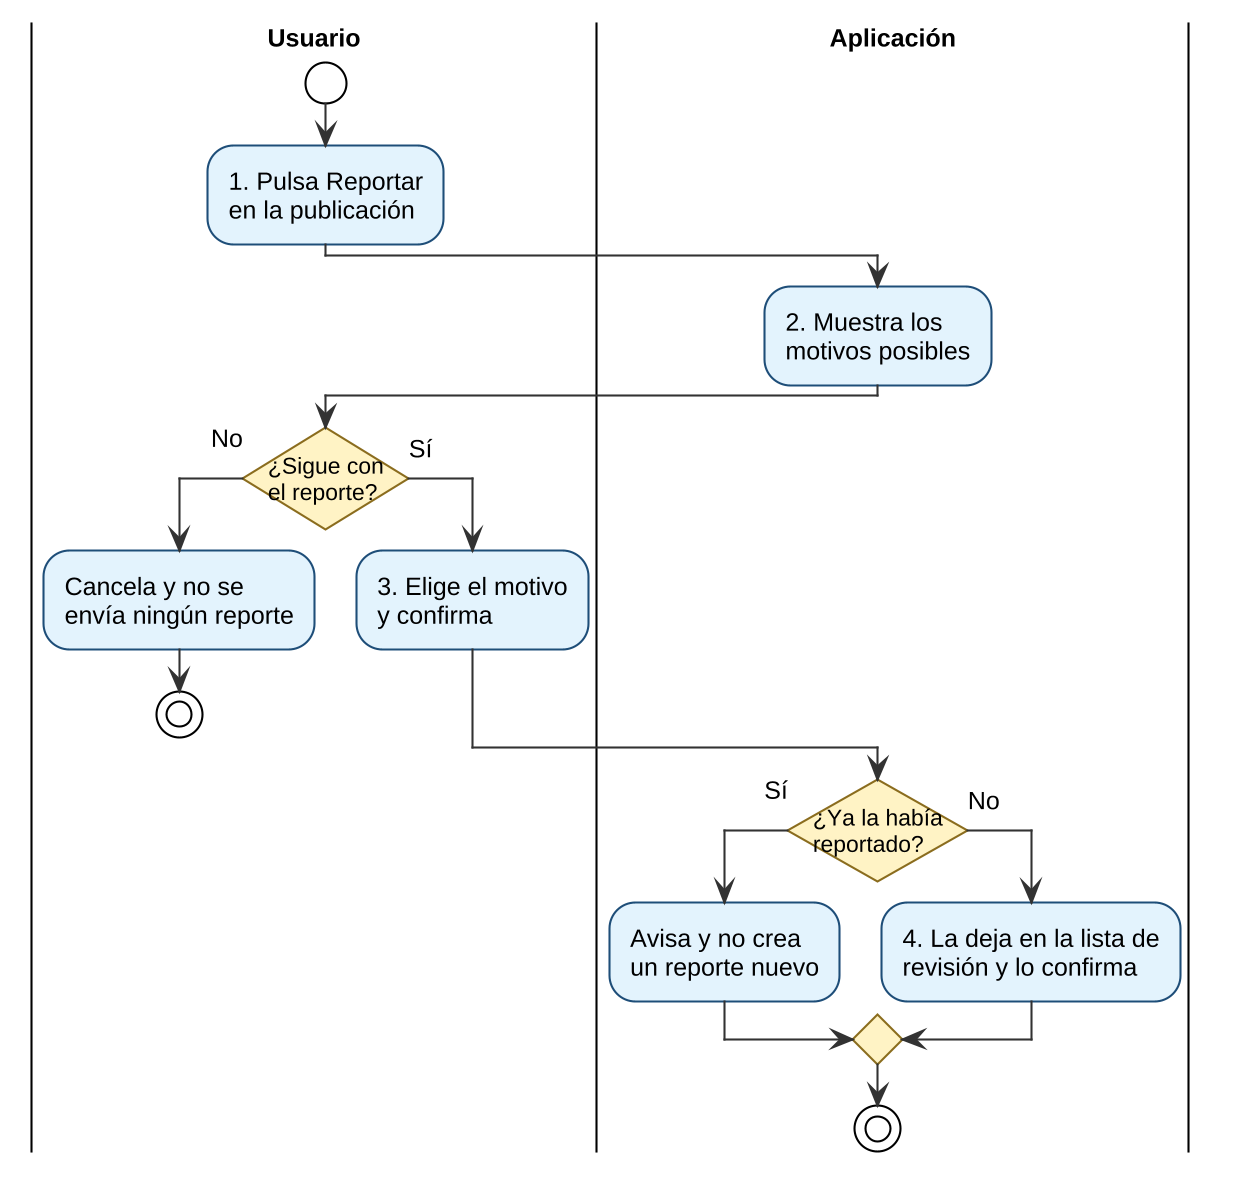
\includegraphics[width=0.78\textwidth,height=0.42\textheight,keepaspectratio]{figuras/diseno/dga_cu22.png}
    \captionof{figure}{Diagrama de Actividades -- CU-22: Reportar una publicación.}
    \label{fig:dga_cu22}
\end{center}

\noindent\begin{minipage}{\linewidth}
\textbf{Descripción Esencial Expandida del Caso de Uso}
\par\vspace{0.2cm}
\noindent
{\renewcommand{\arraystretch}{1.25}\setstretch{1}\small
\begin{tabular}{|>{\raggedright\arraybackslash}p{2.9cm}|>{\raggedright\arraybackslash}p{12.1cm}|}
    \hline
    \rowcolor[HTML]{EFEFEF} \textbf{Propósito} & Avisar al administrador de una publicación o foto inapropiada o peligrosa. \\ \hline
    \textbf{Tipo} & Primario \\ \hline
    \textbf{Actores} & Atleta Híbrido \\ \hline
    \textbf{Requerimientos} & R08, R11 \\ \hline
    \textbf{Precondiciones} & El usuario inició sesión y tiene el plan premium. Ve la publicación en su muro. \\ \hline
    \textbf{Poscondiciones} & La publicación queda en la lista de revisión del administrador (CU-11). \\ \hline
\end{tabular}

\vspace{0.15cm}
\noindent
\begin{tabular}{|>{\raggedright\arraybackslash}p{7.5cm}|>{\raggedright\arraybackslash}p{7.5cm}|}
    \hline
    \rowcolor[HTML]{D9E1F2} \multicolumn{2}{|c|}{\textbf{Curso Normal de los Eventos}} \\ \hline
    \rowcolor[HTML]{EFEFEF} \multicolumn{1}{|c|}{\textbf{Usuario}} & \multicolumn{1}{c|}{\textbf{Respuesta del Sistema}} \\ \hline
        1. Pulsa Reportar en la publicación. & 2. Muestra los motivos posibles. \\ \hline
        3. Elige el motivo y confirma. & 4. Deja la publicación en la lista de revisión y confirma el reporte. \\ \hline
    \rowcolor[HTML]{F2D9D9} \multicolumn{2}{|c|}{\textbf{Cursos Alternos}} \\ \hline
    \rowcolor[HTML]{EFEFEF} \multicolumn{1}{|c|}{\textbf{Usuario}} & \multicolumn{1}{c|}{\textbf{Respuesta del Sistema}} \\ \hline
        3. Si se arrepiente, puede cancelar y no se envía ningún reporte. &  \\ \hline
         & 4. Si ya la había reportado, avisa y no crea un reporte nuevo. \\ \hline
\end{tabular}
}
\end{minipage}
\vspace{0.4cm}

\subsubsection{CU-23. Ver el muro de la comunidad}

\textbf{Diagrama de Actividades}
\begin{center}
    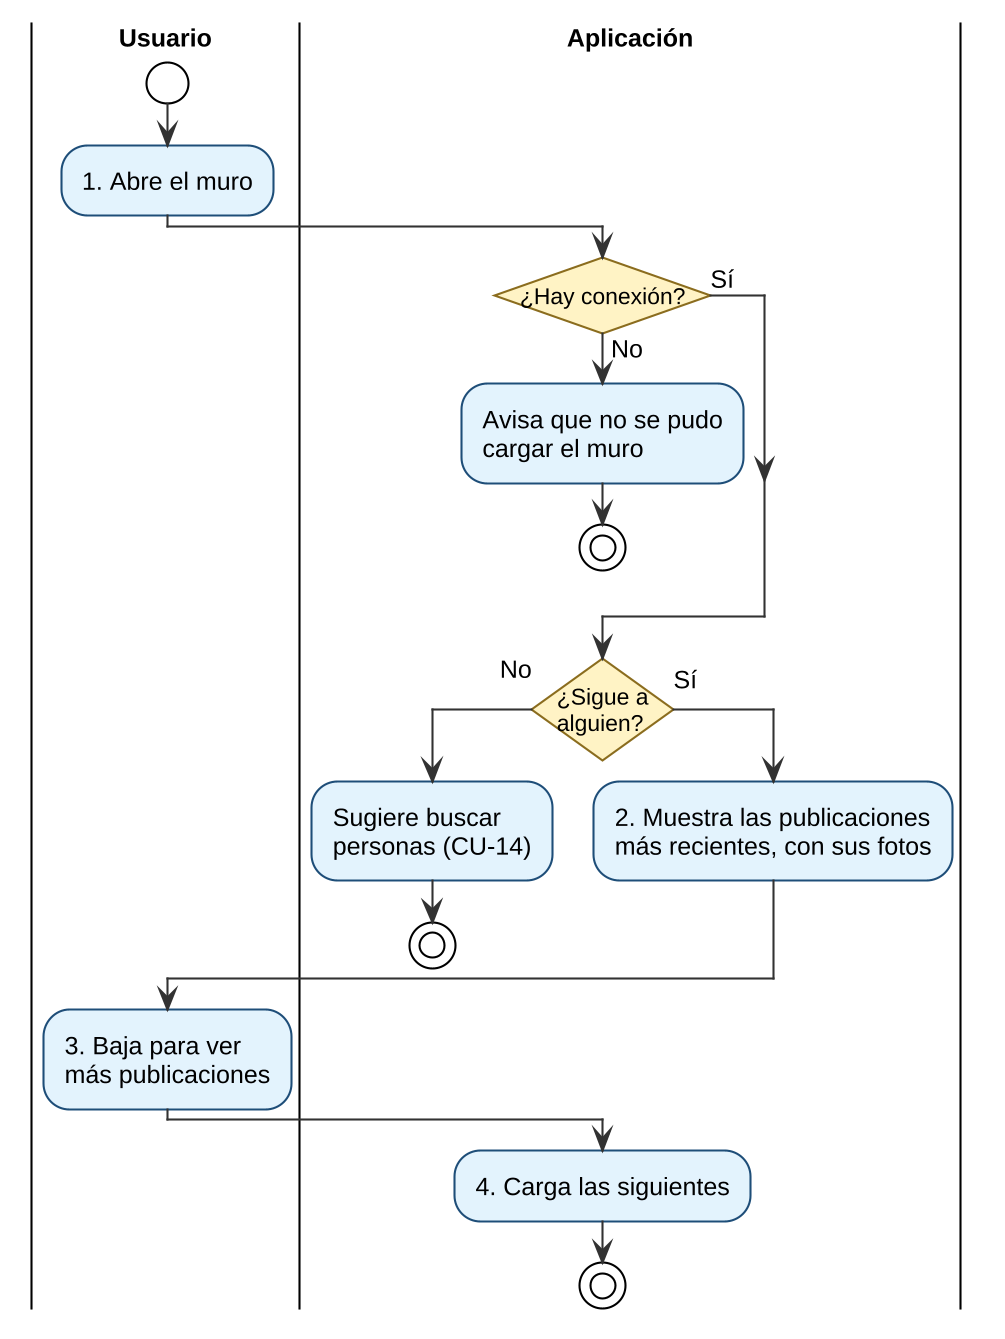
\includegraphics[width=0.78\textwidth,height=0.42\textheight,keepaspectratio]{figuras/diseno/dga_cu23.png}
    \captionof{figure}{Diagrama de Actividades -- CU-23: Ver el muro de la comunidad.}
    \label{fig:dga_cu23}
\end{center}

\noindent\begin{minipage}{\linewidth}
\textbf{Descripción Esencial Expandida del Caso de Uso}
\par\vspace{0.2cm}
\noindent
{\renewcommand{\arraystretch}{1.25}\setstretch{1}\small
\begin{tabular}{|>{\raggedright\arraybackslash}p{2.9cm}|>{\raggedright\arraybackslash}p{12.1cm}|}
    \hline
    \rowcolor[HTML]{EFEFEF} \textbf{Propósito} & Ver lo que publican las personas que el atleta sigue. \\ \hline
    \textbf{Tipo} & Primario \\ \hline
    \textbf{Actores} & Atleta Híbrido \\ \hline
    \textbf{Requerimientos} & R08 \\ \hline
    \textbf{Precondiciones} & El usuario inició sesión y tiene el plan premium. \\ \hline
    \textbf{Poscondiciones} & El atleta ve las publicaciones. Desde ahí puede agregarlas (CU-13) o reportarlas (CU-22). \\ \hline
\end{tabular}

\vspace{0.15cm}
\noindent
\begin{tabular}{|>{\raggedright\arraybackslash}p{7.5cm}|>{\raggedright\arraybackslash}p{7.5cm}|}
    \hline
    \rowcolor[HTML]{D9E1F2} \multicolumn{2}{|c|}{\textbf{Curso Normal de los Eventos}} \\ \hline
    \rowcolor[HTML]{EFEFEF} \multicolumn{1}{|c|}{\textbf{Usuario}} & \multicolumn{1}{c|}{\textbf{Respuesta del Sistema}} \\ \hline
        1. Abre el muro. & 2. Muestra las publicaciones más recientes que puede ver, con sus fotos. \\ \hline
        3. Baja para ver más publicaciones. & 4. Carga las siguientes. \\ \hline
    \rowcolor[HTML]{F2D9D9} \multicolumn{2}{|c|}{\textbf{Cursos Alternos}} \\ \hline
    \rowcolor[HTML]{EFEFEF} \multicolumn{1}{|c|}{\textbf{Usuario}} & \multicolumn{1}{c|}{\textbf{Respuesta del Sistema}} \\ \hline
         & 2. Si todavía no sigue a nadie, le sugiere buscar personas (CU-14). \\ \hline
         & 2. Si no hay conexión, avisa que no se pudo cargar el muro. \\ \hline
\end{tabular}
}
\end{minipage}
\vspace{0.4cm}

\subsubsection{CU-24. Contratar el plan premium}

\textbf{Diagrama de Actividades}
\begin{center}
    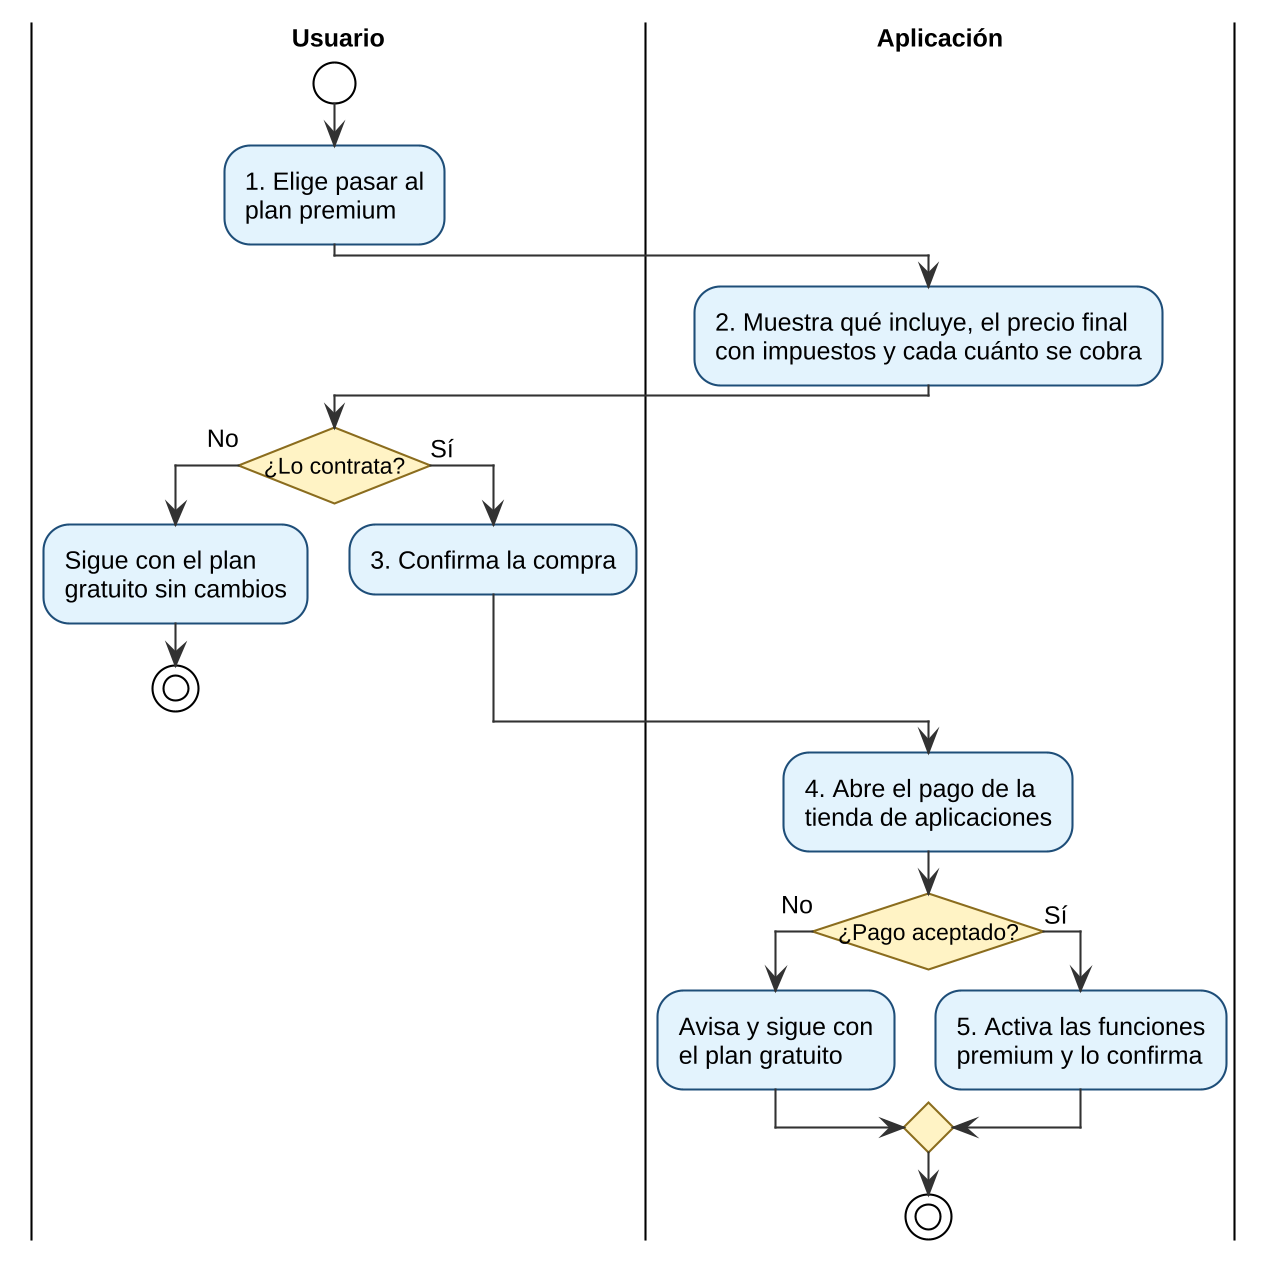
\includegraphics[width=0.78\textwidth,height=0.42\textheight,keepaspectratio]{figuras/diseno/dga_cu24.png}
    \captionof{figure}{Diagrama de Actividades -- CU-24: Contratar el plan premium.}
    \label{fig:dga_cu24}
\end{center}

\noindent\begin{minipage}{\linewidth}
\textbf{Descripción Esencial Expandida del Caso de Uso}
\par\vspace{0.2cm}
\noindent
{\renewcommand{\arraystretch}{1.25}\setstretch{1}\small
\begin{tabular}{|>{\raggedright\arraybackslash}p{2.9cm}|>{\raggedright\arraybackslash}p{12.1cm}|}
    \hline
    \rowcolor[HTML]{EFEFEF} \textbf{Propósito} & Permitir que el usuario acceda a todas las funciones pagando una suscripción. \\ \hline
    \textbf{Tipo} & Primario \\ \hline
    \textbf{Actores} & Atleta Básico \\ \hline
    \textbf{Requerimientos} & R14 \\ \hline
    \textbf{Precondiciones} & El usuario inició sesión y tiene el plan gratuito. \\ \hline
    \textbf{Poscondiciones} & El usuario tiene el plan premium activo. \\ \hline
\end{tabular}

\vspace{0.15cm}
\noindent
\begin{tabular}{|>{\raggedright\arraybackslash}p{7.5cm}|>{\raggedright\arraybackslash}p{7.5cm}|}
    \hline
    \rowcolor[HTML]{D9E1F2} \multicolumn{2}{|c|}{\textbf{Curso Normal de los Eventos}} \\ \hline
    \rowcolor[HTML]{EFEFEF} \multicolumn{1}{|c|}{\textbf{Usuario}} & \multicolumn{1}{c|}{\textbf{Respuesta del Sistema}} \\ \hline
        1. Elige pasar al plan premium. & 2. Muestra qué incluye, el precio final con impuestos y cada cuánto se cobra. \\ \hline
        3. Confirma la compra. & 4. Abre el pago de la tienda de aplicaciones. \\ \hline
         & 5. Activa las funciones premium y lo confirma. \\ \hline
    \rowcolor[HTML]{F2D9D9} \multicolumn{2}{|c|}{\textbf{Cursos Alternos}} \\ \hline
    \rowcolor[HTML]{EFEFEF} \multicolumn{1}{|c|}{\textbf{Usuario}} & \multicolumn{1}{c|}{\textbf{Respuesta del Sistema}} \\ \hline
        3. Si decide no contratar, sigue con el plan gratuito sin cambios. &  \\ \hline
         & 4. Si el pago es rechazado, avisa y el usuario sigue con el plan gratuito. \\ \hline
\end{tabular}
}
\end{minipage}
\vspace{0.4cm}

\subsubsection{CU-25. Cancelar mi suscripción}

\textbf{Diagrama de Actividades}
\begin{center}
    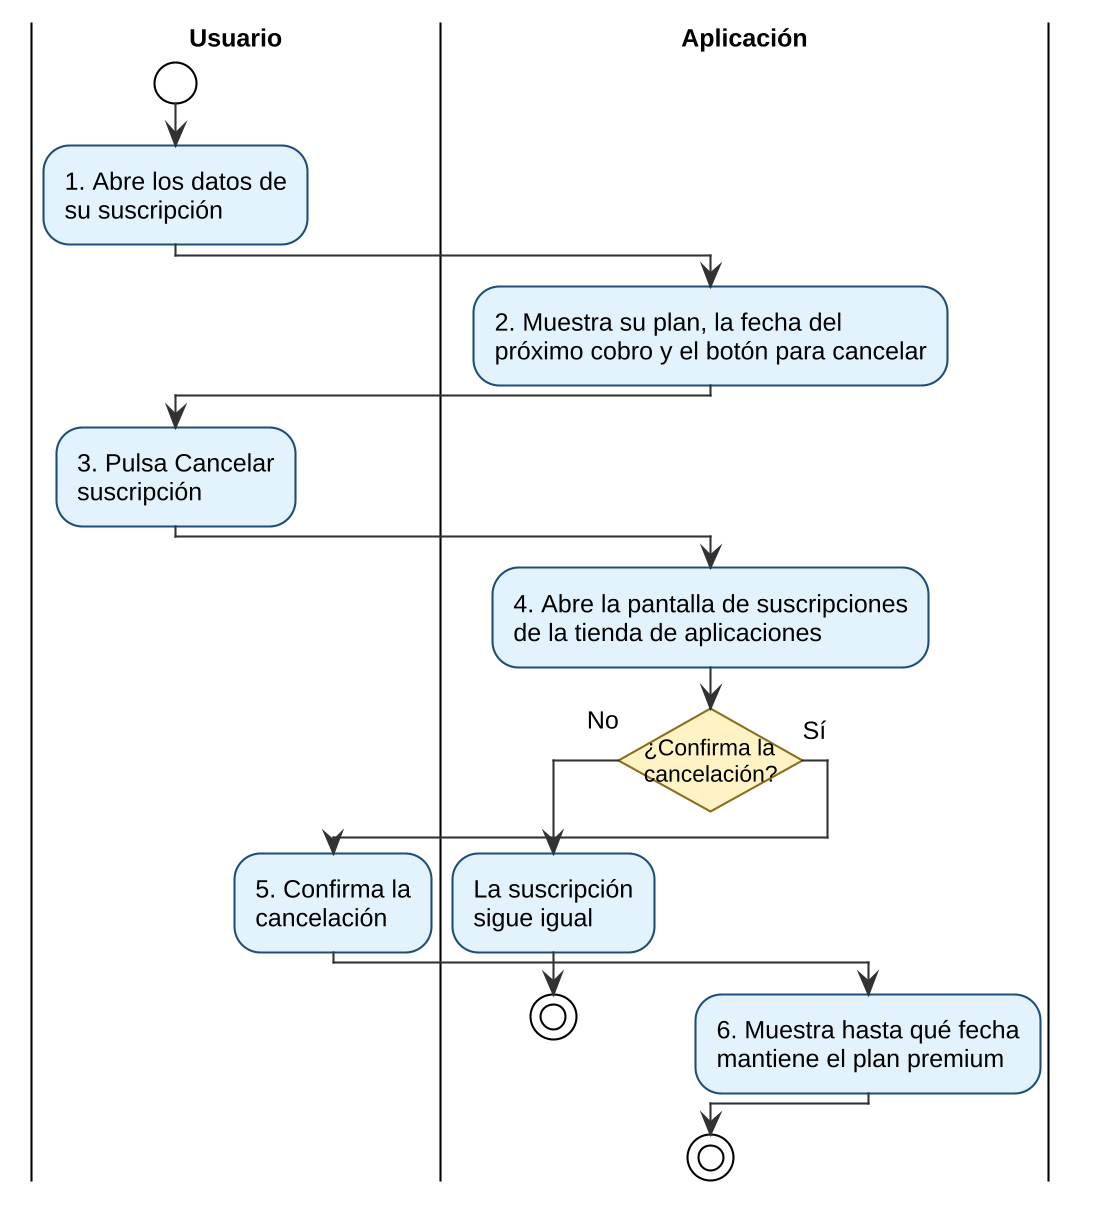
\includegraphics[width=0.78\textwidth,height=0.42\textheight,keepaspectratio]{figuras/diseno/dga_cu25.png}
    \captionof{figure}{Diagrama de Actividades -- CU-25: Cancelar mi suscripción.}
    \label{fig:dga_cu25}
\end{center}

\noindent\begin{minipage}{\linewidth}
\textbf{Descripción Esencial Expandida del Caso de Uso}
\par\vspace{0.2cm}
\noindent
{\renewcommand{\arraystretch}{1.25}\setstretch{1}\small
\begin{tabular}{|>{\raggedright\arraybackslash}p{2.9cm}|>{\raggedright\arraybackslash}p{12.1cm}|}
    \hline
    \rowcolor[HTML]{EFEFEF} \textbf{Propósito} & Permitir que el usuario deje de pagar la suscripción, como pide la Ley N° 19.496. \\ \hline
    \textbf{Tipo} & Primario \\ \hline
    \textbf{Actores} & Atleta Híbrido \\ \hline
    \textbf{Requerimientos} & R14 \\ \hline
    \textbf{Precondiciones} & El usuario inició sesión y tiene el plan premium. \\ \hline
    \textbf{Poscondiciones} & No hay nuevos cobros. Al terminar el periodo pagado, el usuario vuelve al plan gratuito y conserva sus datos. \\ \hline
\end{tabular}

\vspace{0.15cm}
\noindent
\begin{tabular}{|>{\raggedright\arraybackslash}p{7.5cm}|>{\raggedright\arraybackslash}p{7.5cm}|}
    \hline
    \rowcolor[HTML]{D9E1F2} \multicolumn{2}{|c|}{\textbf{Curso Normal de los Eventos}} \\ \hline
    \rowcolor[HTML]{EFEFEF} \multicolumn{1}{|c|}{\textbf{Usuario}} & \multicolumn{1}{c|}{\textbf{Respuesta del Sistema}} \\ \hline
        1. Abre los datos de su suscripción. & 2. Muestra su plan, la fecha del próximo cobro y el botón para cancelar. \\ \hline
        3. Pulsa Cancelar suscripción. & 4. Abre la pantalla de suscripciones de la tienda de aplicaciones. \\ \hline
        5. Confirma la cancelación. & 6. Muestra hasta qué fecha mantiene el plan premium. \\ \hline
    \rowcolor[HTML]{F2D9D9} \multicolumn{2}{|c|}{\textbf{Cursos Alternos}} \\ \hline
    \rowcolor[HTML]{EFEFEF} \multicolumn{1}{|c|}{\textbf{Usuario}} & \multicolumn{1}{c|}{\textbf{Respuesta del Sistema}} \\ \hline
        5. Si se arrepiente, no confirma y la suscripción sigue igual. &  \\ \hline
\end{tabular}
}
\end{minipage}
\vspace{0.4cm}

\subsubsection{CU-26. Aceptar los términos de uso y el aviso legal}

\textbf{Diagrama de Actividades}
\begin{center}
    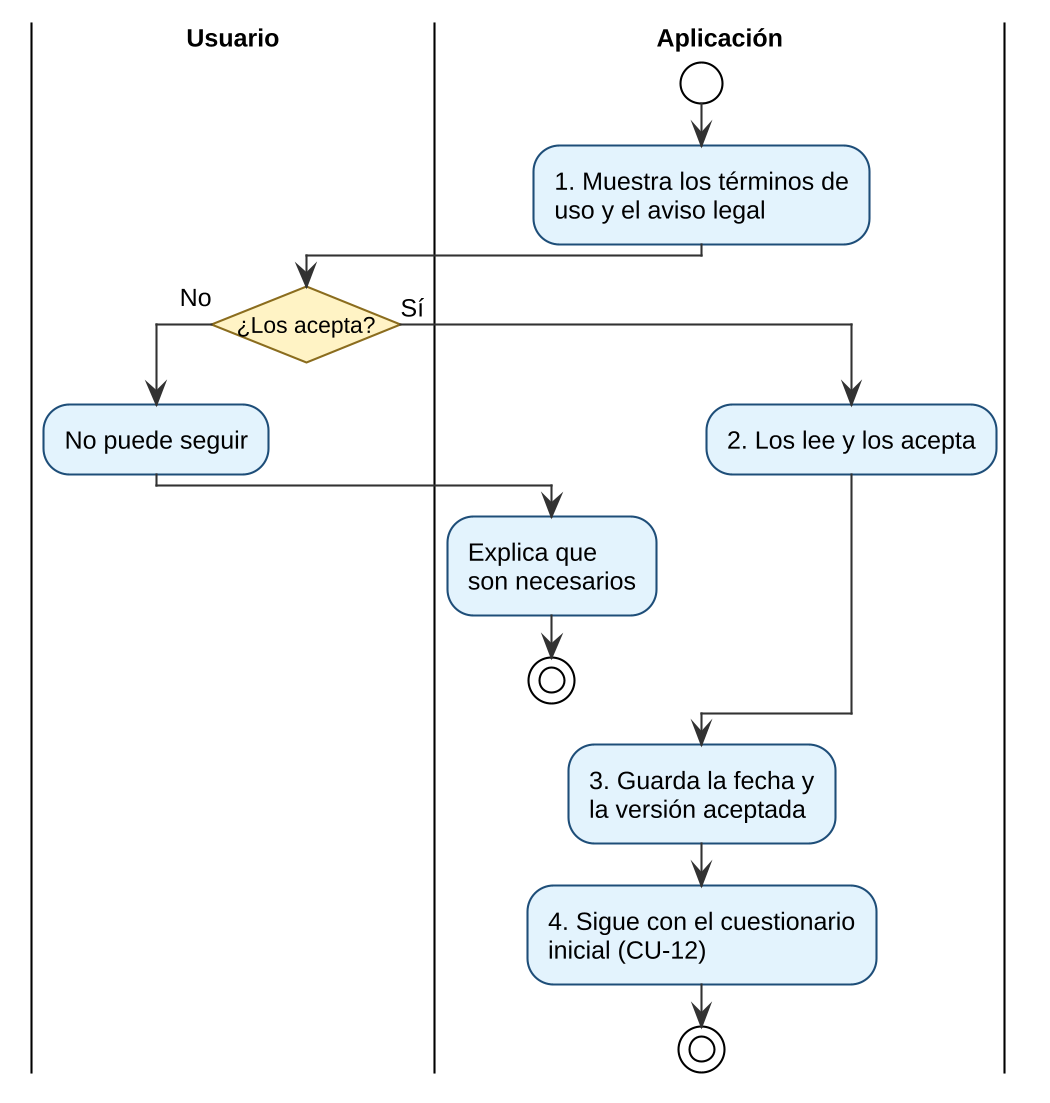
\includegraphics[width=0.78\textwidth,height=0.42\textheight,keepaspectratio]{figuras/diseno/dga_cu26.png}
    \captionof{figure}{Diagrama de Actividades -- CU-26: Aceptar los términos de uso y el aviso legal.}
    \label{fig:dga_cu26}
\end{center}

\noindent\begin{minipage}{\linewidth}
\textbf{Descripción Esencial Expandida del Caso de Uso}
\par\vspace{0.2cm}
\noindent
{\renewcommand{\arraystretch}{1.25}\setstretch{1}\small
\begin{tabular}{|>{\raggedright\arraybackslash}p{2.9cm}|>{\raggedright\arraybackslash}p{12.1cm}|}
    \hline
    \rowcolor[HTML]{EFEFEF} \textbf{Propósito} & Informar al usuario las condiciones de la aplicación y que esta no reemplaza a un profesional de la salud. \\ \hline
    \textbf{Tipo} & Primario \\ \hline
    \textbf{Actores} & Atleta Básico, Atleta Híbrido \\ \hline
    \textbf{Requerimientos} & R15 \\ \hline
    \textbf{Precondiciones} & El usuario está creando su cuenta. \\ \hline
    \textbf{Poscondiciones} & Queda registro de lo que aceptó el usuario. \\ \hline
\end{tabular}

\vspace{0.15cm}
\noindent
\begin{tabular}{|>{\raggedright\arraybackslash}p{7.5cm}|>{\raggedright\arraybackslash}p{7.5cm}|}
    \hline
    \rowcolor[HTML]{D9E1F2} \multicolumn{2}{|c|}{\textbf{Curso Normal de los Eventos}} \\ \hline
    \rowcolor[HTML]{EFEFEF} \multicolumn{1}{|c|}{\textbf{Usuario}} & \multicolumn{1}{c|}{\textbf{Respuesta del Sistema}} \\ \hline
         & 1. Muestra los términos de uso y el aviso legal. \\ \hline
        2. Los lee y los acepta. & 3. Guarda la fecha y la versión aceptada. \\ \hline
         & 4. Sigue con el cuestionario inicial (CU-12). \\ \hline
    \rowcolor[HTML]{F2D9D9} \multicolumn{2}{|c|}{\textbf{Cursos Alternos}} \\ \hline
    \rowcolor[HTML]{EFEFEF} \multicolumn{1}{|c|}{\textbf{Usuario}} & \multicolumn{1}{c|}{\textbf{Respuesta del Sistema}} \\ \hline
         & 1. Si los términos cambian más adelante, los vuelve a mostrar la próxima vez que el usuario entre. \\ \hline
        2. Si no los acepta, la aplicación explica que son necesarios y no permite seguir. &  \\ \hline
\end{tabular}
}
\end{minipage}
\vspace{0.4cm}

\subsubsection{CU-27. Crear una receta}

\textbf{Diagrama de Actividades}
\begin{center}
    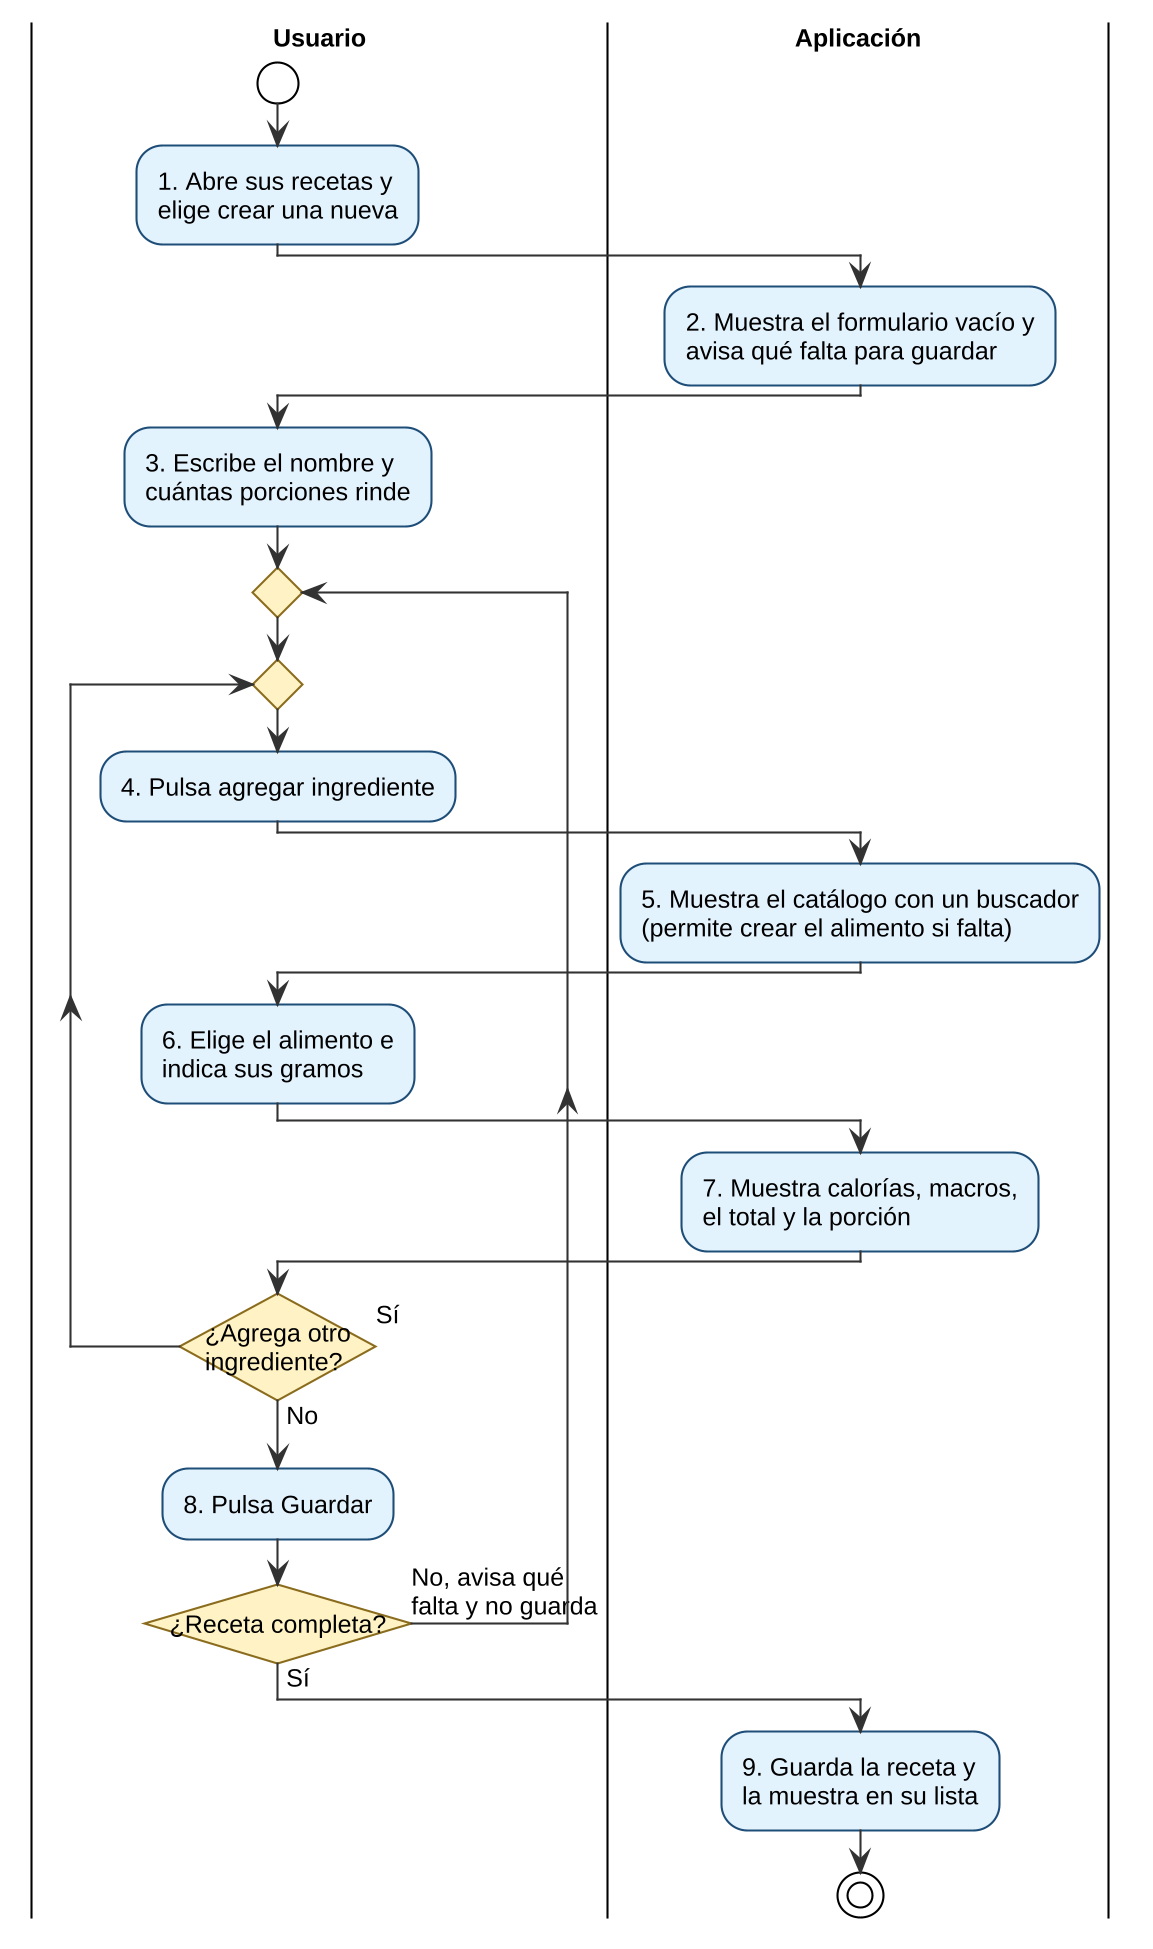
\includegraphics[width=0.9\textwidth,height=0.76\textheight,keepaspectratio]{figuras/diseno/dga_cu27.png}
    \captionof{figure}{Diagrama de Actividades -- CU-27: Crear una receta.}
    \label{fig:dga_cu27}
\end{center}

\noindent\begin{minipage}{\linewidth}
\textbf{Descripción Esencial Expandida del Caso de Uso}
\par\vspace{0.2cm}
\noindent
{\renewcommand{\arraystretch}{1.25}\setstretch{1}\small
\begin{tabular}{|>{\raggedright\arraybackslash}p{2.9cm}|>{\raggedright\arraybackslash}p{12.1cm}|}
    \hline
    \rowcolor[HTML]{EFEFEF} \textbf{Propósito} & Guardar una receta propia, con sus ingredientes y porciones, para volver a registrarla con un solo paso o compartirla. \\ \hline
    \textbf{Tipo} & Primario \\ \hline
    \textbf{Actores} & Atleta Básico, Atleta Híbrido \\ \hline
    \textbf{Requerimientos} & R04 \\ \hline
    \textbf{Precondiciones} & El usuario inició sesión en la aplicación. \\ \hline
    \textbf{Poscondiciones} & La receta queda guardada en el módulo de nutrición del atleta y se puede encontrar al buscar alimentos (CU-06). Un Atleta Híbrido puede publicarla (CU-09). \\ \hline
\end{tabular}

\vspace{0.15cm}
\noindent
\begin{tabular}{|>{\raggedright\arraybackslash}p{7.5cm}|>{\raggedright\arraybackslash}p{7.5cm}|}
    \hline
    \rowcolor[HTML]{D9E1F2} \multicolumn{2}{|c|}{\textbf{Curso Normal de los Eventos}} \\ \hline
    \rowcolor[HTML]{EFEFEF} \multicolumn{1}{|c|}{\textbf{Usuario}} & \multicolumn{1}{c|}{\textbf{Respuesta del Sistema}} \\ \hline
        1. Abre sus recetas y elige crear una nueva. & 2. Muestra el formulario vacío y avisa qué falta para poder guardar. \\ \hline
        3. Escribe el nombre y cuántas porciones rinde. &  \\ \hline
        4. Pulsa agregar ingrediente. & 5. Muestra el catálogo de alimentos con un buscador. \\ \hline
        6. Elige un alimento e indica cuántos gramos lleva. & 7. Muestra sus calorías y sus macronutrientes, y actualiza el total y lo que aporta cada porción. \\ \hline
        8. Repite los pasos 4 a 7 con cada ingrediente y pulsa Guardar. & 9. Revisa que la receta esté completa, la guarda y la muestra en su lista de recetas. \\ \hline
    \rowcolor[HTML]{F2D9D9} \multicolumn{2}{|c|}{\textbf{Cursos Alternos}} \\ \hline
    \rowcolor[HTML]{EFEFEF} \multicolumn{1}{|c|}{\textbf{Usuario}} & \multicolumn{1}{c|}{\textbf{Respuesta del Sistema}} \\ \hline
         & 5. Si el alimento no está en el catálogo, permite crearlo desde la misma búsqueda y lo agrega a la receta. \\ \hline
        7. Si se equivoca con un ingrediente, lo quita o cambia sus gramos, y el total se recalcula. &  \\ \hline
         & 9. Si falta el nombre, las porciones, algún ingrediente o los gramos de uno de ellos, no deja guardar y avisa qué falta. \\ \hline
\end{tabular}
}
\end{minipage}
\vspace{0.4cm}

\subsection{Diseño Técnico}
Esta sección aborda la estructura técnica interna del sistema, detallando cómo se organizan y relacionan las entidades de información, tanto a nivel de persistencia en base de datos como a nivel de la lógica de negocio en el backend.

\subsubsection{Modelo de Datos}

Para guardar la información de la aplicación se usará \textbf{MongoDB}, una base de datos NoSQL orientada a documentos. En vez de tablas, MongoDB organiza los datos en \textbf{colecciones} de \textbf{documentos}, que se guardan en formato BSON (JSON binario). Cada documento puede tener una estructura distinta, lo que se ajusta bien a los datos deportivos, donde una sesión de fuerza puede tener 3 ejercicios y otra 7, cada uno con distinta cantidad de series.
\\\\
El modelo sigue dos reglas simples:
\begin{itemize}
    \item \textbf{Embeber lo que se usa junto:} La información que siempre se consulta en conjunto se guarda dentro del mismo documento. Por ejemplo, las series de cada ejercicio quedan dentro de la sesión de fuerza, y los alimentos de una comida quedan dentro de la comida. Así, una sola consulta trae todo lo necesario.
    \item \textbf{Referenciar lo que se comparte o crece mucho:} Los datos que usan muchos documentos, como el catálogo de ejercicios o de alimentos, tienen su propia colección y se referencian por su identificador (\texttt{ObjectId}). Lo mismo pasa con la telemetría segundo a segundo, que se guarda en una colección de series temporales para no superar el tamaño máximo de un documento (16 MB).
\end{itemize}

Con estas reglas, el modelo queda formado por 15 colecciones, que se resumen en la Tabla \ref{tab:colecciones}.
\begin{table}[h!]
    \centering
    \renewcommand{\arraystretch}{1.3}
    \begin{tabular}{|p{3.0cm}|p{3.9cm}|p{7.5cm}|}
        \hline
        \rowcolor[HTML]{EFEFEF}
        \textbf{Módulo} & \textbf{Colección} & \textbf{Qué guarda} \\ \hline
        Identidad y acceso & \texttt{users} & Usuarios, con su perfil y sus integraciones embebidas. \\ \hline
        Registro diario & \texttt{dailyLogs} & Metas del día y reportes de sensaciones. \\ \hline
        Fuerza & \texttt{exercises} & Catálogo de ejercicios. \\ \hline
        Fuerza y cardio & \texttt{workouts} & Sesiones de fuerza (con ejercicios y series) y de resistencia. \\ \hline
        Cardio & \texttt{telemetry} & Serie temporal con los datos segundo a segundo. \\ \hline
        Nutrición & \texttt{foodItems} & Catálogo de alimentos, con su código de barras. \\ \hline
        Nutrición & \texttt{meals} & Comidas, con sus alimentos embebidos. \\ \hline
        Fatiga & \texttt{fatigueSnapshots} & Cálculo diario de carga y fatiga, con sus alertas. \\ \hline
        Nutrición y comunidad & \texttt{recipes} & Recetas propias o agregadas desde la comunidad, con sus ingredientes. \\ \hline
        Comunidad & \texttt{posts} & Publicaciones de sesiones, rutas y comidas en la red social. \\ \hline
        Perfil y plan & \texttt{trainingPlans} & Plan semanal sugerido de cada usuario y sus ajustes. \\ \hline
        Red social & \texttt{follows} & Relaciones entre seguidores. \\ \hline
        Red social y fuerza & \texttt{routines} & Rutinas de fuerza propias o agregadas desde la comunidad. \\ \hline
        Red social y cardio & \texttt{routes} & Rutas propias o agregadas desde la comunidad. \\ \hline
        Administración & \texttt{moderationLogs} & Acciones de moderación del administrador. \\ \hline
    \end{tabular}
    \caption{Colecciones del modelo de datos en MongoDB.}
    \label{tab:colecciones}
\end{table}
\textbf{Índices principales}

Para que las consultas más frecuentes sean rápidas, se definen los siguientes índices:
\begin{itemize}
    \item \texttt{users.email}: único, para el inicio de sesión.
    \item \texttt{dailyLogs (userId, date)} y \texttt{fatigueSnapshots (userId, date)}: únicos, para que haya un solo documento por usuario y día.
    \item \texttt{workouts (userId, startedAt)} y \texttt{meals (userId, consumedAt)}: para armar la línea de tiempo diaria y mensual.
    \item \texttt{foodItems.barcode}: único y disperso (solo para los alimentos que tienen código), para la lectura de códigos de barras.
    \item \texttt{telemetry}: colección de series temporales, con \texttt{timestamp} como campo de tiempo y \texttt{meta.workoutId} como campo de agrupación.
    \item \texttt{follows (followerId, followeeId)}: único, para que no se repita una misma relación entre seguidores.
    
    \item \texttt{posts (authorId, createdAt)}: para armar el muro con las publicaciones más recientes de las personas que el usuario sigue.
    \item \texttt{routes.startPoint}: índice geoespacial (\texttt{2dsphere}), para buscar rutas cercanas.
    \item \texttt{trainingPlans (userId, weekStart)}: para obtener el plan de la semana actual.
\end{itemize}

Las funciones de la red social que quedan para después del MVP, como los récords de tramo y los retos entre seguidores, necesitarán colecciones adicionales (por ejemplo \texttt{segments}, \texttt{segmentEfforts} y \texttt{challenges}), que se diseñarán en esas versiones.

\subsubsection{Diccionario de Datos}
A continuación se detalla la estructura de cada colección. Los campos que están dentro de un subdocumento se escriben con punto (por ejemplo, \texttt{profile.weightKg}), y los arreglos de subdocumentos se marcan con corchetes (por ejemplo, \texttt{sets[].reps}). Todos los documentos tienen un campo \texttt{\_id} de tipo \texttt{ObjectId}, que MongoDB genera automáticamente.
\\\\
\noindent\textbf{Colección: users} \\
Descripción: Guarda la identidad del usuario, su perfil físico y sus conexiones con servicios externos. El perfil y las integraciones van embebidos porque siempre se leen junto con el usuario.
{\footnotesize
\renewcommand{\arraystretch}{1.2}
\begin{longtable}{|>{\raggedright\arraybackslash}p{4.7cm}|>{\raggedright\arraybackslash}p{1.8cm}|>{\raggedright\arraybackslash}p{2.3cm}|>{\raggedright\arraybackslash}p{5.4cm}|}
    \hline
    \rowcolor[HTML]{EFEFEF}
    \textbf{Campo} & \textbf{Tipo} & \textbf{Atributo} & \textbf{Descripción} \\ \hline
    \endhead
    \_id & ObjectId & Obligatorio & Identificador único del usuario. \\ \hline
    email & String & Único & Correo de contacto e inicio de sesión. \\ \hline
    passwordHash & String & Obligatorio & Contraseña protegida con un algoritmo de hash. \\ \hline
    firstName & String & Obligatorio & Nombre del usuario. \\ \hline
    lastName & String & Obligatorio & Apellido del usuario. \\ \hline
    role & String & Obligatorio & Rol (ATHLETE\_FREE, ATHLETE\_PREMIUM o ADMIN). \\ \hline
    consent.\allowbreak dataProcessing & Boolean & Obligatorio & Aceptación del tratamiento de datos sensibles. \\ \hline
    consent.\allowbreak grantedAt & Date & Obligatorio & Fecha de la aceptación. \\ \hline
    consent.\allowbreak termsVersion & String & Obligatorio & Versión de los términos de uso aceptada. \\ \hline
    subscription & Object & Opcional & Datos de la suscripción al plan premium. \\ \hline
    subscription.\allowbreak status & String & Obligatorio & Estado (ACTIVE, CANCELED o EXPIRED). \\ \hline
    subscription.\allowbreak store & String & Obligatorio & Tienda donde se contrató (GOOGLE\_PLAY o APP\_STORE). \\ \hline
    subscription.\allowbreak expiresAt & Date & Obligatorio & Fecha en que termina el periodo pagado. \\ \hline
    subscription.\allowbreak purchaseToken & String & Obligatorio & Comprobante de compra entregado por la tienda. \\ \hline
    deviceTokens[] & Array & Opcional & Identificadores del teléfono del usuario para enviar notificaciones. \\ \hline
    profile & Object & Embebido & Perfil físico del usuario. \\ \hline
    profile.\allowbreak birthDate & Date & Obligatorio & Fecha de nacimiento. \\ \hline
    profile.\allowbreak gender & String & Obligatorio & Género (M, F u OTHER). \\ \hline
    profile.\allowbreak heightCm & Double & Obligatorio & Estatura en centímetros. \\ \hline
    profile.\allowbreak weightKg & Double & Obligatorio & Peso en kilogramos. \\ \hline
    profile.\allowbreak restingHeartRate & Int32 & Opcional & Frecuencia cardíaca en reposo. \\ \hline
    profile.\allowbreak maxHeartRate & Int32 & Opcional & Frecuencia cardíaca máxima. \\ \hline
    profile.\allowbreak activityLevel & String & Obligatorio & Nivel de actividad física. \\ \hline
    profile.\allowbreak primaryGoal & String & Obligatorio & Meta principal (fuerza, resistencia o recomposición). \\ \hline
    profile.\allowbreak experienceLevel & String & Obligatorio & Nivel declarado (BEGINNER, INTERMEDIATE o ADVANCED). \\ \hline
    profile.\allowbreak orientation & String & Obligatorio & Orientación calculada a partir del cuestionario (STRENGTH, ENDURANCE o BALANCED). \\ \hline
    profile.\allowbreak availableDays & Int32 & Obligatorio & Días por semana que puede entrenar. \\ \hline
    profile.\allowbreak equipment[]\allowbreak  & Array & Opcional & Equipamiento disponible (gimnasio, mancuernas, bicicleta, reloj, etc.). \\ \hline
    profile.\allowbreak disciplines[]\allowbreak  & Array & Obligatorio & Disciplinas que practica (fuerza, ciclismo, running o trekking). \\ \hline
    integrations[]\allowbreak  & Array & Embebido & Conexiones con servicios externos. \\ \hline
    integrations[]\allowbreak .\allowbreak provider & String & Obligatorio & Proveedor (APPLE\_HEALTH, HEALTH\_CONNECT, GARMIN o POLAR). \\ \hline
    integrations[]\allowbreak .\allowbreak accessTokenEnc & BinData & Obligatorio & Token de acceso cifrado (AES-256). \\ \hline
    integrations[]\allowbreak .\allowbreak refreshTokenEnc & BinData & Opcional & Token de renovación cifrado. \\ \hline
    integrations[]\allowbreak .\allowbreak tokenExpiresAt & Date & Obligatorio & Vencimiento del token. \\ \hline
    integrations[]\allowbreak .\allowbreak isActive & Boolean & Obligatorio & Indica si la conexión está activa. \\ \hline
    createdAt & Date & Obligatorio & Fecha de registro. \\ \hline
    updatedAt & Date & Obligatorio & Fecha de la última actualización. \\ \hline
    deletedAt & Date & Opcional & Fecha de eliminación lógica. \\ \hline
\end{longtable}
}
\noindent\textbf{Colección: dailyLogs} \\
Descripción: Representa un día del usuario. Guarda sus metas de calorías y macronutrientes y sus reportes de sensaciones. Hay un solo documento por usuario y fecha.
{\footnotesize
\renewcommand{\arraystretch}{1.2}
\begin{longtable}{|>{\raggedright\arraybackslash}p{4.7cm}|>{\raggedright\arraybackslash}p{1.8cm}|>{\raggedright\arraybackslash}p{2.3cm}|>{\raggedright\arraybackslash}p{5.4cm}|}
    \hline
    \rowcolor[HTML]{EFEFEF}
    \textbf{Campo} & \textbf{Tipo} & \textbf{Atributo} & \textbf{Descripción} \\ \hline
    \endhead
    \_id & ObjectId & Obligatorio & Identificador del registro diario. \\ \hline
    userId & ObjectId & Ref. users & Usuario dueño del registro. \\ \hline
    date & Date & Índice único con userId & Fecha del registro. \\ \hline
    targets.\allowbreak calories & Int32 & Obligatorio & Meta de calorías del día. \\ \hline
    targets.\allowbreak proteinG & Double & Obligatorio & Meta de proteínas (g). \\ \hline
    targets.\allowbreak carbsG & Double & Obligatorio & Meta de carbohidratos (g). \\ \hline
    targets.\allowbreak fatG & Double & Obligatorio & Meta de grasas (g). \\ \hline
    subjectiveReports[]\allowbreak  & Array & Embebido & Reportes de sensaciones del día. \\ \hline
    subjectiveReports[]\allowbreak .\allowbreak rpeGeneral & Int32 & Obligatorio & Esfuerzo percibido general (1 a 10). \\ \hline
    subjectiveReports[]\allowbreak .\allowbreak sleepQuality & Int32 & Opcional & Calidad del sueño (1 a 10). \\ \hline
    subjectiveReports[]\allowbreak .\allowbreak muscleSoreness & Int32 & Opcional & Dolor muscular (1 a 10). \\ \hline
    subjectiveReports[]\allowbreak .\allowbreak energyLevel & Int32 & Opcional & Nivel de energía (1 a 10). \\ \hline
    subjectiveReports[]\allowbreak .\allowbreak giDiscomfort & Boolean & Opcional & Presencia de malestar digestivo. \\ \hline
    subjectiveReports[]\allowbreak .\allowbreak freeNotes & String & Opcional & Notas libres. \\ \hline
    subjectiveReports[]\allowbreak .\allowbreak relatedTo & Object & Opcional & Entrenamiento o comida al que pertenece la nota (tipo e identificador). \\ \hline
    subjectiveReports[]\allowbreak .\allowbreak createdAt & Date & Obligatorio & Fecha del reporte. \\ \hline
    notes & String & Opcional & Notas del día. \\ \hline
    createdAt & Date & Obligatorio & Fecha de creación. \\ \hline
    updatedAt & Date & Obligatorio & Fecha de modificación. \\ \hline
\end{longtable}
}
\noindent\textbf{Colección: exercises} \\
Descripción: Catálogo de ejercicios de fuerza, tanto oficiales como creados por los usuarios. Los grupos musculares van dentro del documento, porque son pocos y casi no cambian.
{\footnotesize
\renewcommand{\arraystretch}{1.2}
\begin{longtable}{|>{\raggedright\arraybackslash}p{4.7cm}|>{\raggedright\arraybackslash}p{1.8cm}|>{\raggedright\arraybackslash}p{2.3cm}|>{\raggedright\arraybackslash}p{5.4cm}|}
    \hline
    \rowcolor[HTML]{EFEFEF}
    \textbf{Campo} & \textbf{Tipo} & \textbf{Atributo} & \textbf{Descripción} \\ \hline
    \endhead
    \_id & ObjectId & Obligatorio & Identificador del ejercicio. \\ \hline
    name & String & Índice & Nombre del ejercicio. \\ \hline
    muscleGroups.\allowbreak primary & String & Obligatorio & Grupo muscular principal. \\ \hline
    muscleGroups.\allowbreak secondary & String & Opcional & Grupo muscular secundario. \\ \hline
    bodyRegion & String & Obligatorio & Región del cuerpo (UPPER, LOWER, CORE o FULL\_BODY). \\ \hline
    movementPattern & String & Obligatorio & Patrón de movimiento (PUSH, PULL, SQUAT, etc.). \\ \hline
    equipment & String & Obligatorio & Equipamiento requerido. \\ \hline
    measureType & String & Obligatorio & Forma de medir: REPS (repeticiones) o TIME (isométricos). \\ \hline
    isBodyweight & Boolean & Obligatorio & Indica si usa el peso corporal como carga (calistenia). \\ \hline
    description & String & Opcional & Instrucciones técnicas. \\ \hline
    isOfficial & Boolean & Obligatorio & Indica si pertenece al catálogo oficial. \\ \hline
    createdBy & ObjectId & Ref. users, opcional & Usuario que lo creó, si es personalizado. \\ \hline
    isActive & Boolean & Obligatorio & Estado del ejercicio. \\ \hline
    createdAt & Date & Obligatorio & Fecha de creación. \\ \hline
\end{longtable}
}
\noindent\textbf{Colección: workouts} \\
Descripción: Guarda todas las sesiones de entrenamiento. El campo \texttt{type} indica si es de fuerza o de resistencia, y según eso el documento tiene unos campos u otros. Esta flexibilidad es una de las ventajas del modelo de documentos.
{\footnotesize
\renewcommand{\arraystretch}{1.2}
\begin{longtable}{|>{\raggedright\arraybackslash}p{4.7cm}|>{\raggedright\arraybackslash}p{1.8cm}|>{\raggedright\arraybackslash}p{2.3cm}|>{\raggedright\arraybackslash}p{5.4cm}|}
    \hline
    \rowcolor[HTML]{EFEFEF}
    \textbf{Campo} & \textbf{Tipo} & \textbf{Atributo} & \textbf{Descripción} \\ \hline
    \endhead
    \multicolumn{4}{|l|}{\cellcolor[HTML]{E3F2FD}\textbf{Campos comunes}} \\ \hline
    \_id & ObjectId & Obligatorio & Identificador de la sesión. \\ \hline
    userId & ObjectId & Ref. users, índice & Usuario que realizó la sesión. \\ \hline
    dailyLogId & ObjectId & Ref. dailyLogs & Día al que pertenece la sesión. \\ \hline
    type & String & Obligatorio & Tipo de sesión (STRENGTH o CARDIO). \\ \hline
    startedAt & Date & Índice con userId & Inicio de la sesión. \\ \hline
    finishedAt & Date & Opcional & Fin de la sesión. \\ \hline
    sessionRpe & Int32 & Obligatorio & Esfuerzo percibido de la sesión (1 a 10), indicado por el usuario o estimado por la aplicación. \\ \hline
    rpeSource & String & Obligatorio & Origen del RPE: USER (lo indicó el usuario) o ESTIMATED (lo estimó la aplicación). \\ \hline
    loadAu & Double & Obligatorio & Carga de la sesión en unidades arbitrarias: RPE por minutos. \\ \hline
    notes & String & Opcional & Notas de la sesión. \\ \hline
    createdAt & Date & Obligatorio & Fecha de registro. \\ \hline
    \multicolumn{4}{|l|}{\cellcolor[HTML]{E3F2FD}\textbf{Solo cuando type = STRENGTH}} \\ \hline
    trainingType & String & Opcional & Tipo de fuerza (MAX\_STRENGTH, HYPERTROPHY, POWER, MUSCULAR\_ENDURANCE, ISOMETRIC o CALISTHENICS). \\ \hline
    inputMethod & String & Obligatorio & Forma de registro (MANUAL o NLP). \\ \hline
    nlpRawInput & String & Opcional & Texto original si se registró con lenguaje natural. \\ \hline
    totalVolumeKg & Double & Obligatorio & Volumen total (series por repeticiones por peso), solo informativo. \\ \hline
    exercises[]\allowbreak  & Array & Embebido & Ejercicios realizados en la sesión. \\ \hline
    exercises[]\allowbreak .\allowbreak exerciseId & ObjectId & Ref. exercises & Ejercicio del catálogo. \\ \hline
    exercises[]\allowbreak .\allowbreak exerciseName & String & Obligatorio & Copia del nombre, para mostrarlo sin consultar el catálogo. \\ \hline
    exercises[]\allowbreak .\allowbreak order & Int32 & Obligatorio & Orden de ejecución. \\ \hline
    exercises[]\allowbreak .\allowbreak sets[]\allowbreak  & Array & Embebido & Series del ejercicio. \\ \hline
    exercises[]\allowbreak .\allowbreak sets[]\allowbreak .\allowbreak reps & Int32 & Opcional & Repeticiones (no aplica en isométricos). \\ \hline
    exercises[]\allowbreak .\allowbreak sets[]\allowbreak .\allowbreak durationSec & Int32 & Opcional & Duración en segundos (isométricos). \\ \hline
    exercises[]\allowbreak .\allowbreak sets[]\allowbreak .\allowbreak weightKg & Double & Obligatorio & Carga en kilogramos, o lastre en calistenia. \\ \hline
    exercises[]\allowbreak .\allowbreak sets[]\allowbreak .\allowbreak rpe & Double & Opcional & Esfuerzo percibido de la serie. \\ \hline
    exercises[]\allowbreak .\allowbreak sets[]\allowbreak .\allowbreak restSec & Int32 & Opcional & Descanso en segundos. \\ \hline
    exercises[]\allowbreak .\allowbreak sets[]\allowbreak .\allowbreak isWarmup & Boolean & Opcional & Indica si fue una serie de calentamiento. \\ \hline
    \multicolumn{4}{|l|}{\cellcolor[HTML]{E3F2FD}\textbf{Solo cuando type = CARDIO}} \\ \hline
    discipline & String & Obligatorio & Disciplina (CYCLING, RUNNING o TREKKING). \\ \hline
    durationSec & Int32 & Obligatorio & Duración activa en segundos. \\ \hline
    distanceM & Double & Obligatorio & Distancia total en metros. \\ \hline
    avgSpeedKmh & Double & Opcional & Velocidad promedio. \\ \hline
    elevationGainM & Double & Opcional & Desnivel positivo en metros. \\ \hline
    dataSource & String & Obligatorio & Origen de los datos (PHONE\_GPS, HEALTH\_BROKER o FIT\_FILE). \\ \hline
    dataConfidence & String & Obligatorio & Nivel de confianza del dato (LOW, MEDIUM o HIGH). \\ \hline
    heartRate.\allowbreak avg & Int32 & Opcional & Frecuencia cardíaca promedio. \\ \hline
    heartRate.\allowbreak max & Int32 & Opcional & Frecuencia cardíaca máxima. \\ \hline
    heartRate.\allowbreak activeCalories & Int32 & Opcional & Calorías activas (kcal). \\ \hline
    power.\allowbreak avgWatts & Int32 & Opcional & Potencia promedio (W). \\ \hline
    power.\allowbreak maxWatts & Int32 & Opcional & Potencia máxima (W). \\ \hline
    power.\allowbreak normalizedPower & Int32 & Opcional & Potencia normalizada (NP). \\ \hline
    power.\allowbreak avgCadence & Int32 & Opcional & Cadencia promedio. \\ \hline
    power.\allowbreak tss & Double & Opcional & Training Stress Score, solo informativo. \\ \hline
    fitFileUrl & String & Opcional & Ubicación en S3 del archivo .fit original. \\ \hline
\end{longtable}
}
\noindent\textbf{Colección: telemetry} \\
Descripción: Colección de series temporales (time series) de MongoDB. Cada documento es una medición segundo a segundo de una sesión de resistencia. Se separa de \texttt{workouts} porque una sesión larga puede tener miles de puntos y un documento no puede superar los 16 MB.
{\footnotesize
\renewcommand{\arraystretch}{1.2}
\begin{longtable}{|>{\raggedright\arraybackslash}p{4.7cm}|>{\raggedright\arraybackslash}p{1.8cm}|>{\raggedright\arraybackslash}p{2.3cm}|>{\raggedright\arraybackslash}p{5.4cm}|}
    \hline
    \rowcolor[HTML]{EFEFEF}
    \textbf{Campo} & \textbf{Tipo} & \textbf{Atributo} & \textbf{Descripción} \\ \hline
    \endhead
    \_id & ObjectId & Obligatorio & Identificador de la medición. \\ \hline
    timestamp & Date & Campo de tiempo & Momento de la medición. \\ \hline
    meta.\allowbreak workoutId & ObjectId & Ref. workouts & Sesión a la que pertenece la medición. \\ \hline
    meta.\allowbreak userId & ObjectId & Ref. users & Usuario dueño de la sesión. \\ \hline
    meta.\allowbreak source & String & Obligatorio & Origen (FIT\_FILE o HEALTH\_BROKER). \\ \hline
    heartRate & Int32 & Opcional & Frecuencia cardíaca. \\ \hline
    powerWatts & Int32 & Opcional & Potencia (W). \\ \hline
    cadence & Int32 & Opcional & Cadencia. \\ \hline
    speedKmh & Double & Opcional & Velocidad. \\ \hline
    altitudeM & Double & Opcional & Altitud en metros. \\ \hline
    location & Object & Opcional & Posición GPS en formato GeoJSON (punto). \\ \hline
\end{longtable}
}
\noindent\textbf{Colección: foodItems} \\
Descripción: Catálogo de alimentos, ya sea cargados desde una base externa (como OpenFoodFacts), creados por los usuarios o estimados por la IA.
{\footnotesize
\renewcommand{\arraystretch}{1.2}
\begin{longtable}{|>{\raggedright\arraybackslash}p{4.7cm}|>{\raggedright\arraybackslash}p{1.8cm}|>{\raggedright\arraybackslash}p{2.3cm}|>{\raggedright\arraybackslash}p{5.4cm}|}
    \hline
    \rowcolor[HTML]{EFEFEF}
    \textbf{Campo} & \textbf{Tipo} & \textbf{Atributo} & \textbf{Descripción} \\ \hline
    \endhead
    \_id & ObjectId & Obligatorio & Identificador del alimento. \\ \hline
    name & String & Índice de texto & Nombre del alimento. \\ \hline
    brand & String & Opcional & Marca o fabricante. \\ \hline
    servingSizeG & Double & Obligatorio & Tamaño de la porción estándar (g). \\ \hline
    per100g.\allowbreak calories & Double & Obligatorio & Calorías por cada 100 g. \\ \hline
    per100g.\allowbreak proteinG & Double & Obligatorio & Proteínas por cada 100 g. \\ \hline
    per100g.\allowbreak carbsG & Double & Obligatorio & Carbohidratos por cada 100 g. \\ \hline
    per100g.\allowbreak fatG & Double & Obligatorio & Grasas por cada 100 g. \\ \hline
    per100g.\allowbreak fiberG & Double & Opcional & Fibra por cada 100 g. \\ \hline
    source & String & Obligatorio & Origen (OPEN\_FOOD\_FACTS, USER o AI). \\ \hline
    barcode & String & Único, opcional & Código de barras EAN o UPC. \\ \hline
    isActive & Boolean & Obligatorio & Estado del alimento. \\ \hline
    createdAt & Date & Obligatorio & Fecha de alta. \\ \hline
\end{longtable}
}
\noindent\textbf{Colección: meals} \\
Descripción: Registro de cada comida. Los alimentos consumidos van dentro del documento, junto con los totales ya calculados, para mostrar el diario sin consultas adicionales.
{\footnotesize
\renewcommand{\arraystretch}{1.2}
\begin{longtable}{|>{\raggedright\arraybackslash}p{4.7cm}|>{\raggedright\arraybackslash}p{1.8cm}|>{\raggedright\arraybackslash}p{2.3cm}|>{\raggedright\arraybackslash}p{5.4cm}|}
    \hline
    \rowcolor[HTML]{EFEFEF}
    \textbf{Campo} & \textbf{Tipo} & \textbf{Atributo} & \textbf{Descripción} \\ \hline
    \endhead
    \_id & ObjectId & Obligatorio & Identificador de la comida. \\ \hline
    userId & ObjectId & Ref. users, índice & Usuario que registró la comida. \\ \hline
    dailyLogId & ObjectId & Ref. dailyLogs & Día al que descuenta los macronutrientes. \\ \hline
    mealType & String & Obligatorio & Momento (BREAKFAST, LUNCH, DINNER o SNACK). \\ \hline
    inputMethod & String & Obligatorio & Forma de registro (MANUAL, TEXT, PHOTO o BARCODE). \\ \hline
    aiConfidenceScore & Double & Opcional & Seguridad de la estimación de la IA (0 a 100). \\ \hline
    items[]\allowbreak  & Array & Embebido & Alimentos de la comida. \\ \hline
    items[]\allowbreak .\allowbreak foodItemId & ObjectId & Ref. foodItems & Alimento del catálogo. \\ \hline
    items[]\allowbreak .\allowbreak name & String & Obligatorio & Copia del nombre del alimento. \\ \hline
    items[]\allowbreak .\allowbreak quantityG & Double & Obligatorio & Gramos consumidos. \\ \hline
    items[]\allowbreak .\allowbreak calories & Double & Obligatorio & Calorías aportadas. \\ \hline
    items[]\allowbreak .\allowbreak proteinG & Double & Obligatorio & Proteínas aportadas. \\ \hline
    items[]\allowbreak .\allowbreak carbsG & Double & Obligatorio & Carbohidratos aportados. \\ \hline
    items[]\allowbreak .\allowbreak fatG & Double & Obligatorio & Grasas aportadas. \\ \hline
    totals.\allowbreak calories & Double & Obligatorio & Calorías totales de la comida. \\ \hline
    totals.\allowbreak proteinG & Double & Obligatorio & Proteínas totales. \\ \hline
    totals.\allowbreak carbsG & Double & Obligatorio & Carbohidratos totales. \\ \hline
    totals.\allowbreak fatG & Double & Obligatorio & Grasas totales. \\ \hline
    recipeRef.\allowbreak recipeId & ObjectId & Ref. recipes, opcional & Receta de la comunidad, si se importó. \\ \hline
    recipeRef.\allowbreak scaleFactor & Double & Opcional & Factor con el que se ajustó la receta. \\ \hline
    notes & String & Opcional & Notas de preparación. \\ \hline
    consumedAt & Date & Índice con userId & Momento en que se comió. \\ \hline
    createdAt & Date & Obligatorio & Fecha de registro. \\ \hline
\end{longtable}
}
\noindent\textbf{Colección: fatigueSnapshots} \\
Descripción: Guarda el cálculo diario de carga y fatiga de cada usuario. Las alertas que genera el cálculo van dentro del mismo documento.
{\footnotesize
\renewcommand{\arraystretch}{1.2}
\begin{longtable}{|>{\raggedright\arraybackslash}p{4.7cm}|>{\raggedright\arraybackslash}p{1.8cm}|>{\raggedright\arraybackslash}p{2.3cm}|>{\raggedright\arraybackslash}p{5.4cm}|}
    \hline
    \rowcolor[HTML]{EFEFEF}
    \textbf{Campo} & \textbf{Tipo} & \textbf{Atributo} & \textbf{Descripción} \\ \hline
    \endhead
    \_id & ObjectId & Obligatorio & Identificador del cálculo. \\ \hline
    userId & ObjectId & Ref. users & Usuario evaluado. \\ \hline
    date & Date & Índice único con userId & Fecha evaluada. \\ \hline
    strength.\allowbreak ctl & Double & Obligatorio & Carga crónica de fuerza. \\ \hline
    strength.\allowbreak atl & Double & Obligatorio & Carga aguda de fuerza. \\ \hline
    strength.\allowbreak tsb & Double & Obligatorio & Balance de forma (TSB) de fuerza. \\ \hline
    cardio.\allowbreak ctl & Double & Obligatorio & Carga crónica de resistencia. \\ \hline
    cardio.\allowbreak atl & Double & Obligatorio & Carga aguda de resistencia. \\ \hline
    cardio.\allowbreak tsb & Double & Obligatorio & Balance de forma (TSB) de resistencia. \\ \hline
    total.\allowbreak ctl & Double & Obligatorio & Carga crónica total (fuerza más cardio). \\ \hline
    total.\allowbreak atl & Double & Obligatorio & Carga aguda total (fuerza más cardio). \\ \hline
    total.\allowbreak tsb & Double & Obligatorio & Balance de forma (TSB) total. \\ \hline
    crossFatigueIndex & Double & Opcional & Índice de fatiga cruzada: razón ATL/CTL de la carga total (Tabla \ref{tab:def_operativas}). Queda vacío mientras no hay 28 días de historial. \\ \hline
    calculatedAt & Date & Obligatorio & Momento del cálculo. \\ \hline
    alerts[]\allowbreak  & Array & Embebido & Alertas generadas por el cálculo. \\ \hline
    alerts[]\allowbreak .\allowbreak alertType & String & Obligatorio & Tipo de alerta (CROSS\_FATIGUE, etc.). \\ \hline
    alerts[]\allowbreak .\allowbreak severity & String & Obligatorio & Severidad (INFO, WARNING o CRITICAL). \\ \hline
    alerts[]\allowbreak .\allowbreak message & String & Obligatorio & Mensaje de la alerta. \\ \hline
    alerts[]\allowbreak .\allowbreak suggestion & String & Opcional & Sugerencia de ajuste del entrenamiento. \\ \hline
    alerts[]\allowbreak .\allowbreak isRead & Boolean & Obligatorio & Indica si el usuario ya la leyó. \\ \hline
    alerts[]\allowbreak .\allowbreak isPushSent & Boolean & Obligatorio & Indica si se envió la notificación push. \\ \hline
    alerts[]\allowbreak .\allowbreak createdAt & Date & Obligatorio & Fecha de la alerta. \\ \hline
\end{longtable}
}
\noindent\textbf{Colección: recipes} \\
Descripción: Recetas creadas por el usuario (CU-27) o agregadas desde una publicación de la comunidad (CU-08). Los ingredientes van dentro del documento, en el orden de preparación.
{\footnotesize
\renewcommand{\arraystretch}{1.2}
\begin{longtable}{|>{\raggedright\arraybackslash}p{4.7cm}|>{\raggedright\arraybackslash}p{1.8cm}|>{\raggedright\arraybackslash}p{2.3cm}|>{\raggedright\arraybackslash}p{5.4cm}|}
    \hline
    \rowcolor[HTML]{EFEFEF}
    \textbf{Campo} & \textbf{Tipo} & \textbf{Atributo} & \textbf{Descripción} \\ \hline
    \endhead
    \_id & ObjectId & Obligatorio & Identificador de la receta. \\ \hline
    authorId & ObjectId & Ref. users & Usuario que creó la receta. \\ \hline
    source.\allowbreak recipeId & ObjectId & Ref. recipes, opcional & Receta original, si fue agregada desde la comunidad. \\ \hline
    source.\allowbreak authorId & ObjectId & Ref. users, opcional & Autor de la receta original. \\ \hline
    title & String & Índice de texto & Título de la receta. \\ \hline
    description & String & Opcional & Instrucciones de preparación. \\ \hline
    servings & Int32 & Obligatorio & Porciones que rinde. \\ \hline
    ingredients[]\allowbreak  & Array & Embebido & Ingredientes de la receta. \\ \hline
    ingredients[]\allowbreak .\allowbreak foodItemId & ObjectId & Ref. foodItems & Alimento del catálogo. \\ \hline
    ingredients[]\allowbreak .\allowbreak name & String & Obligatorio & Copia del nombre del alimento. \\ \hline
    ingredients[]\allowbreak .\allowbreak quantityG & Double & Obligatorio & Cantidad en gramos. \\ \hline
    ingredients[]\allowbreak .\allowbreak order & Int32 & Obligatorio & Orden de preparación. \\ \hline
    totals.\allowbreak calories & Double & Obligatorio & Calorías totales de la receta. \\ \hline
    totals.\allowbreak proteinG & Double & Obligatorio & Proteínas totales. \\ \hline
    totals.\allowbreak carbsG & Double & Obligatorio & Carbohidratos totales. \\ \hline
    totals.\allowbreak fatG & Double & Obligatorio & Grasas totales. \\ \hline
    visibility & String & Obligatorio & Visibilidad (PUBLIC o PRIVATE). Una receta nueva parte como PRIVATE. \\ \hline
    isModerated & Boolean & Obligatorio & Indica si fue ocultada por moderación. \\ \hline
    isActive & Boolean & Obligatorio & Estado de la receta. \\ \hline
    createdAt & Date & Obligatorio & Fecha de creación. \\ \hline
    updatedAt & Date & Obligatorio & Fecha de la última edición. \\ \hline
\end{longtable}
}
\noindent\textbf{Colección: posts} \\
Descripción: Publicaciones de la red social. Pueden referirse a una sesión de fuerza, una ruta, una comida o una receta. Pueden incluir hasta 4 fotos. Los videos quedan para después del MVP.
{\footnotesize
\renewcommand{\arraystretch}{1.2}
\begin{longtable}{|>{\raggedright\arraybackslash}p{4.7cm}|>{\raggedright\arraybackslash}p{1.8cm}|>{\raggedright\arraybackslash}p{2.3cm}|>{\raggedright\arraybackslash}p{5.4cm}|}
    \hline
    \rowcolor[HTML]{EFEFEF}
    \textbf{Campo} & \textbf{Tipo} & \textbf{Atributo} & \textbf{Descripción} \\ \hline
    \endhead
    \_id & ObjectId & Obligatorio & Identificador de la publicación. \\ \hline
    authorId & ObjectId & Ref. users & Autor de la publicación. \\ \hline
    postType & String & Obligatorio & Tipo (WORKOUT\_SHARE, ROUTE\_SHARE, MEAL\_SHARE o RECIPE\_SHARE). \\ \hline
    content & String & Obligatorio & Texto de la publicación. \\ \hline
    media[] & Array & Opcional & Fotos de la publicación (máximo 4). \\ \hline
    media[].\allowbreak url & String & Obligatorio & Dirección de la foto en S3. \\ \hline
    media[].\allowbreak thumbUrl & String & Obligatorio & Dirección de la miniatura que se muestra en el muro. \\ \hline
    ref.\allowbreak type & String & Opcional & Tipo de elemento compartido (WORKOUT, ROUTE, MEAL o RECIPE). \\ \hline
    ref.\allowbreak id & ObjectId & Ref. workouts, routes, meals o recipes & Elemento compartido. \\ \hline
    visibility & String & Obligatorio & Alcance (PUBLIC, FOLLOWERS o PRIVATE). \\ \hline
    importsCount & Int32 & Obligatorio & Veces que otros usuarios la agregaron a sus módulos. \\ \hline
    reportsCount & Int32 & Obligatorio & Veces que fue reportada. Las publicaciones con reportes aparecen en la lista de revisión del administrador. \\ \hline
    reports[] & Array & Embebido & Reportes recibidos por la publicación. \\ \hline
    reports[]\allowbreak .\allowbreak reporterId & ObjectId & Obligatorio & Usuario que hizo el reporte (referencia a \texttt{users}). \\ \hline
    reports[]\allowbreak .\allowbreak reason & String & Obligatorio & Motivo del reporte. \\ \hline
    reports[]\allowbreak .\allowbreak status & String & Obligatorio & Estado (PENDING, RESOLVED o DISMISSED). \\ \hline
    reports[]\allowbreak .\allowbreak createdAt & Date & Obligatorio & Fecha del reporte. \\ \hline
    isModerated & Boolean & Obligatorio & Indica si fue ocultada por moderación. \\ \hline
    isActive & Boolean & Obligatorio & Estado de la publicación. \\ \hline
    createdAt & Date & Índice & Fecha de publicación. \\ \hline
\end{longtable}
}
\noindent\textbf{Colección: follows} \\
Descripción: Relaciones entre usuarios de la red social. Cada documento indica que un usuario sigue a otro.
{\footnotesize
\renewcommand{\arraystretch}{1.2}
\begin{longtable}{|>{\raggedright\arraybackslash}p{4.7cm}|>{\raggedright\arraybackslash}p{1.8cm}|>{\raggedright\arraybackslash}p{2.3cm}|>{\raggedright\arraybackslash}p{5.4cm}|}
    \hline
    \rowcolor[HTML]{EFEFEF}
    \textbf{Campo} & \textbf{Tipo} & \textbf{Atributo} & \textbf{Descripción} \\ \hline
    \endhead
    \_id & ObjectId & Obligatorio & Identificador de la relación. \\ \hline
    followerId & ObjectId & Ref. users & Usuario que sigue. \\ \hline
    followeeId & ObjectId & Ref. users & Usuario seguido. \\ \hline
    createdAt & Date & Obligatorio & Fecha en que comenzó a seguirlo. \\ \hline
\end{longtable}
}
\noindent\textbf{Colección: routines} \\
Descripción: Rutinas de fuerza del usuario. Pueden ser creadas por él o agregadas desde una publicación de la comunidad, en cuyo caso guardan una referencia al autor original.
{\footnotesize
\renewcommand{\arraystretch}{1.2}
\begin{longtable}{|>{\raggedright\arraybackslash}p{4.7cm}|>{\raggedright\arraybackslash}p{1.8cm}|>{\raggedright\arraybackslash}p{2.3cm}|>{\raggedright\arraybackslash}p{5.4cm}|}
    \hline
    \rowcolor[HTML]{EFEFEF}
    \textbf{Campo} & \textbf{Tipo} & \textbf{Atributo} & \textbf{Descripción} \\ \hline
    \endhead
    \_id & ObjectId & Obligatorio & Identificador de la rutina. \\ \hline
    ownerId & ObjectId & Ref. users & Usuario dueño de la rutina. \\ \hline
    name & String & Obligatorio & Nombre de la rutina (por ejemplo, Rutina de pecho). \\ \hline
    trainingType & String & Opcional & Tipo de fuerza al que apunta. \\ \hline
    exercises[]\allowbreak  & Array & Embebido & Ejercicios de la rutina. \\ \hline
    exercises[]\allowbreak .\allowbreak exerciseId & ObjectId & Ref. exercises & Ejercicio del catálogo. \\ \hline
    exercises[]\allowbreak .\allowbreak exerciseName & String & Obligatorio & Copia del nombre del ejercicio. \\ \hline
    exercises[]\allowbreak .\allowbreak order & Int32 & Obligatorio & Orden en la rutina. \\ \hline
    exercises[]\allowbreak .\allowbreak targetSets & Int32 & Obligatorio & Series sugeridas. \\ \hline
    exercises[]\allowbreak .\allowbreak targetReps & Int32 & Opcional & Repeticiones sugeridas. \\ \hline
    exercises[]\allowbreak .\allowbreak targetDurationSec & Int32 & Opcional & Duración sugerida (isométricos). \\ \hline
    exercises[]\allowbreak .\allowbreak targetWeightKg & Double & Opcional & Carga de referencia. \\ \hline
    source.\allowbreak postId & ObjectId & Ref. posts, opcional & Publicación desde la que se agregó. \\ \hline
    source.\allowbreak authorId & ObjectId & Ref. users, opcional & Autor original de la rutina. \\ \hline
    createdAt & Date & Obligatorio & Fecha de creación. \\ \hline
    updatedAt & Date & Obligatorio & Fecha de la última edición. \\ \hline
\end{longtable}
}
\noindent\textbf{Colección: routes} \\
Descripción: Rutas de cardio del usuario, propias o agregadas desde la comunidad. Al publicarse, se ocultan el inicio y el final del recorrido.
{\footnotesize
\renewcommand{\arraystretch}{1.2}
\begin{longtable}{|>{\raggedright\arraybackslash}p{4.7cm}|>{\raggedright\arraybackslash}p{1.8cm}|>{\raggedright\arraybackslash}p{2.3cm}|>{\raggedright\arraybackslash}p{5.4cm}|}
    \hline
    \rowcolor[HTML]{EFEFEF}
    \textbf{Campo} & \textbf{Tipo} & \textbf{Atributo} & \textbf{Descripción} \\ \hline
    \endhead
    \_id & ObjectId & Obligatorio & Identificador de la ruta. \\ \hline
    ownerId & ObjectId & Ref. users & Usuario dueño de la ruta. \\ \hline
    name & String & Obligatorio & Nombre de la ruta. \\ \hline
    discipline & String & Obligatorio & Disciplina (CYCLING, RUNNING o TREKKING). \\ \hline
    distanceM & Double & Obligatorio & Distancia total en metros. \\ \hline
    elevationGainM & Double & Opcional & Desnivel positivo en metros. \\ \hline
    path & Object & Obligatorio & Trazado en formato GeoJSON (línea). \\ \hline
    startPoint & Object & Índice geoespacial & Punto de referencia de la ruta (GeoJSON), para buscar rutas cercanas. \\ \hline
    visibility & String & Obligatorio & Alcance (PUBLIC, FOLLOWERS o PRIVATE). \\ \hline
    source.\allowbreak postId & ObjectId & Ref. posts, opcional & Publicación desde la que se agregó. \\ \hline
    source.\allowbreak authorId & ObjectId & Ref. users, opcional & Autor original de la ruta. \\ \hline
    createdAt & Date & Obligatorio & Fecha de creación. \\ \hline
\end{longtable}
}
\noindent\textbf{Colección: trainingPlans} \\
Descripción: Plan semanal sugerido para cada usuario. Se genera a partir de una plantilla según su perfil y guarda los ajustes que se le hacen, para que el usuario pueda ver por qué cambió.
{\footnotesize
\renewcommand{\arraystretch}{1.2}
\begin{longtable}{|>{\raggedright\arraybackslash}p{4.7cm}|>{\raggedright\arraybackslash}p{1.8cm}|>{\raggedright\arraybackslash}p{2.3cm}|>{\raggedright\arraybackslash}p{5.4cm}|}
    \hline
    \rowcolor[HTML]{EFEFEF}
    \textbf{Campo} & \textbf{Tipo} & \textbf{Atributo} & \textbf{Descripción} \\ \hline
    \endhead
    \_id & ObjectId & Obligatorio & Identificador del plan. \\ \hline
    userId & ObjectId & Ref. users & Usuario al que pertenece el plan. \\ \hline
    profileSnapshot.\allowbreak level & String & Obligatorio & Nivel usado para generar el plan. \\ \hline
    profileSnapshot.\allowbreak orientation & String & Obligatorio & Orientación usada para generar el plan. \\ \hline
    weekStart & Date & Índice con userId & Primer día de la semana del plan. \\ \hline
    days[]\allowbreak  & Array & Embebido & Días de la semana con su sesión sugerida. \\ \hline
    days[]\allowbreak .\allowbreak dayOfWeek & Int32 & Obligatorio & Día de la semana (1 a 7). \\ \hline
    days[]\allowbreak .\allowbreak sessionType & String & Obligatorio & Tipo de sesión (STRENGTH, CARDIO o REST). \\ \hline
    days[]\allowbreak .\allowbreak routineId & ObjectId & Ref. routines, opcional & Rutina de fuerza sugerida. \\ \hline
    days[]\allowbreak .\allowbreak discipline & String & Opcional & Disciplina de cardio sugerida. \\ \hline
    days[]\allowbreak .\allowbreak targetDurationMin & Int32 & Opcional & Duración sugerida en minutos. \\ \hline
    days[]\allowbreak .\allowbreak notes & String & Opcional & Indicaciones de la sesión. \\ \hline
    status & String & Obligatorio & Estado (ACTIVE o ARCHIVED). \\ \hline
    adjustments[]\allowbreak  & Array & Embebido & Ajustes aplicados al plan. \\ \hline
    adjustments[]\allowbreak .\allowbreak date & Date & Obligatorio & Fecha del ajuste. \\ \hline
    adjustments[]\allowbreak .\allowbreak reason & String & Obligatorio & Motivo (baja adherencia, RPE alto, fatiga o buen progreso). \\ \hline
    adjustments[]\allowbreak .\allowbreak change & String & Obligatorio & Cambio aplicado al volumen sugerido. \\ \hline
    generatedAt & Date & Obligatorio & Fecha de generación. \\ \hline
    updatedAt & Date & Obligatorio & Fecha de la última actualización. \\ \hline
\end{longtable}
}
\noindent\textbf{Colección: moderationLogs} \\
Descripción: Bitácora de las acciones de moderación que realiza el administrador.
{\footnotesize
\renewcommand{\arraystretch}{1.2}
\begin{longtable}{|>{\raggedright\arraybackslash}p{4.7cm}|>{\raggedright\arraybackslash}p{1.8cm}|>{\raggedright\arraybackslash}p{2.3cm}|>{\raggedright\arraybackslash}p{5.4cm}|}
    \hline
    \rowcolor[HTML]{EFEFEF}
    \textbf{Campo} & \textbf{Tipo} & \textbf{Atributo} & \textbf{Descripción} \\ \hline
    \endhead
    \_id & ObjectId & Obligatorio & Identificador del registro. \\ \hline
    adminId & ObjectId & Ref. users & Administrador que realizó la acción. \\ \hline
    targetType & String & Obligatorio & Tipo de elemento (POST o RECIPE). \\ \hline
    targetId & ObjectId & Ref. posts o recipes & Elemento afectado. \\ \hline
    action & String & Obligatorio & Acción realizada (HIDE, DELETE, etc.). \\ \hline
    reason & String & Opcional & Motivo de la acción. \\ \hline
    executedAt & Date & Obligatorio & Fecha de la acción. \\ \hline
\end{longtable}
}

\subsubsection{Flujos de Procesos}
A continuación se presenta el diagrama de secuencia de cada caso de uso. Estos diagramas muestran cómo se comunican las partes del sistema, es decir, la aplicación en Flutter, la API en NestJS, la base de datos MongoDB y los servicios externos. A diferencia de los casos de uso, aquí sí se usan términos técnicos, porque esta información es para quien va a construir el sistema.
\\\\
Las flechas continuas son llamadas y las punteadas son respuestas. Los recuadros \texttt{alt} muestran caminos que se excluyen entre sí, que corresponden a los cursos alternos del Diseño Funcional, y los recuadros \texttt{opt} muestran pasos que ocurren solo en algunos casos. Todas las llamadas a la API van por HTTPS y llevan el token JWT del usuario, por lo que no se repite en cada diagrama. Las llamadas pueden cambiar a medida que avance el prototipo evolutivo.
\noindent\begin{minipage}{\linewidth}
\textbf{CU-01. Anotar una sesión de fuerza}

Para el caso de uso CU-01 se genera el diagrama de secuencia que se muestra en la Figura \ref{fig:sec_cu01}.
\begin{center}
    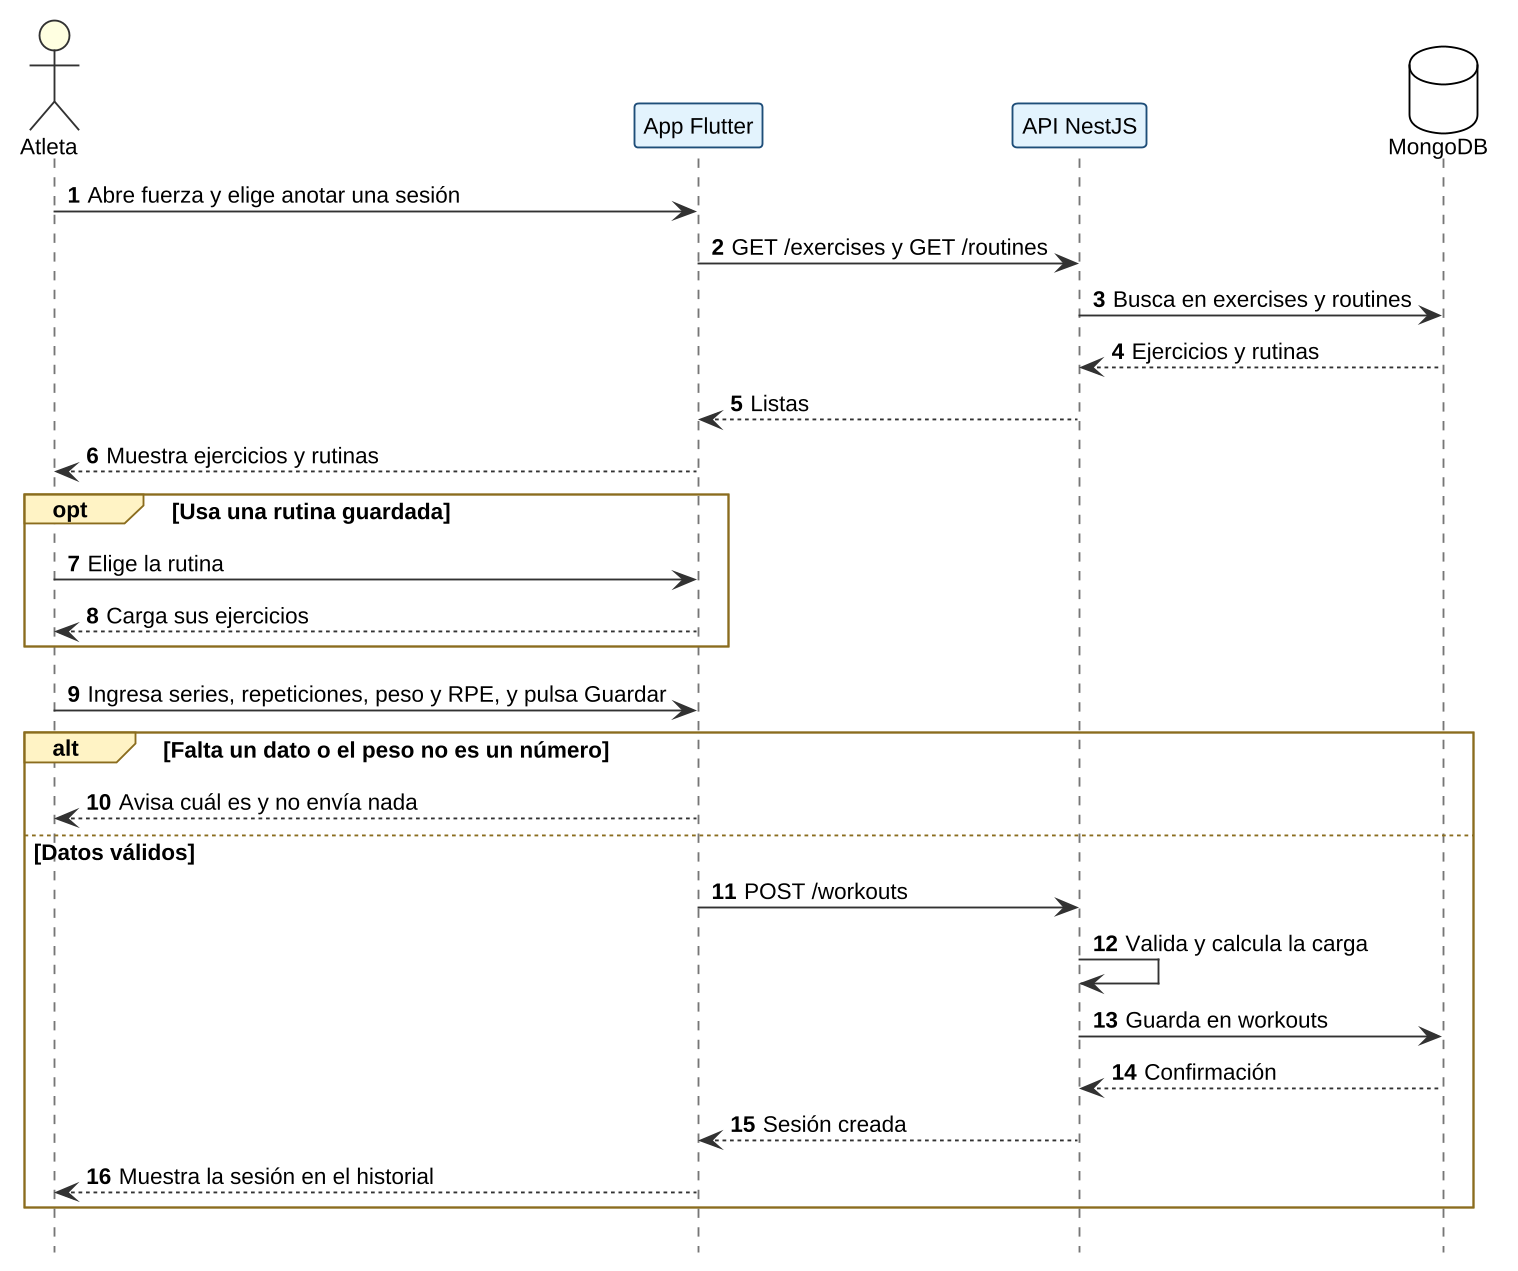
\includegraphics[width=0.95\textwidth,height=0.6\textheight,keepaspectratio]{figuras/secuencia/sec_cu01.png}
    \captionof{figure}{Diagrama de Secuencia -- CU-01: Anotar una sesión de fuerza.}
    \label{fig:sec_cu01}
\end{center}
La aplicación carga el catálogo de ejercicios y las rutinas del usuario. Cuando este pulsa Guardar, la propia aplicación revisa que no falten datos antes de enviarlos. El backend vuelve a validarlos, calcula la carga de la sesión y la guarda en \texttt{workouts}.
\end{minipage}
\vspace{0.6cm}

\noindent\begin{minipage}{\linewidth}
\textbf{CU-02. Contar mi sesión de fuerza con mis palabras}

Para el caso de uso CU-02 se genera el diagrama de secuencia que se muestra en la Figura \ref{fig:sec_cu02}.
\begin{center}
    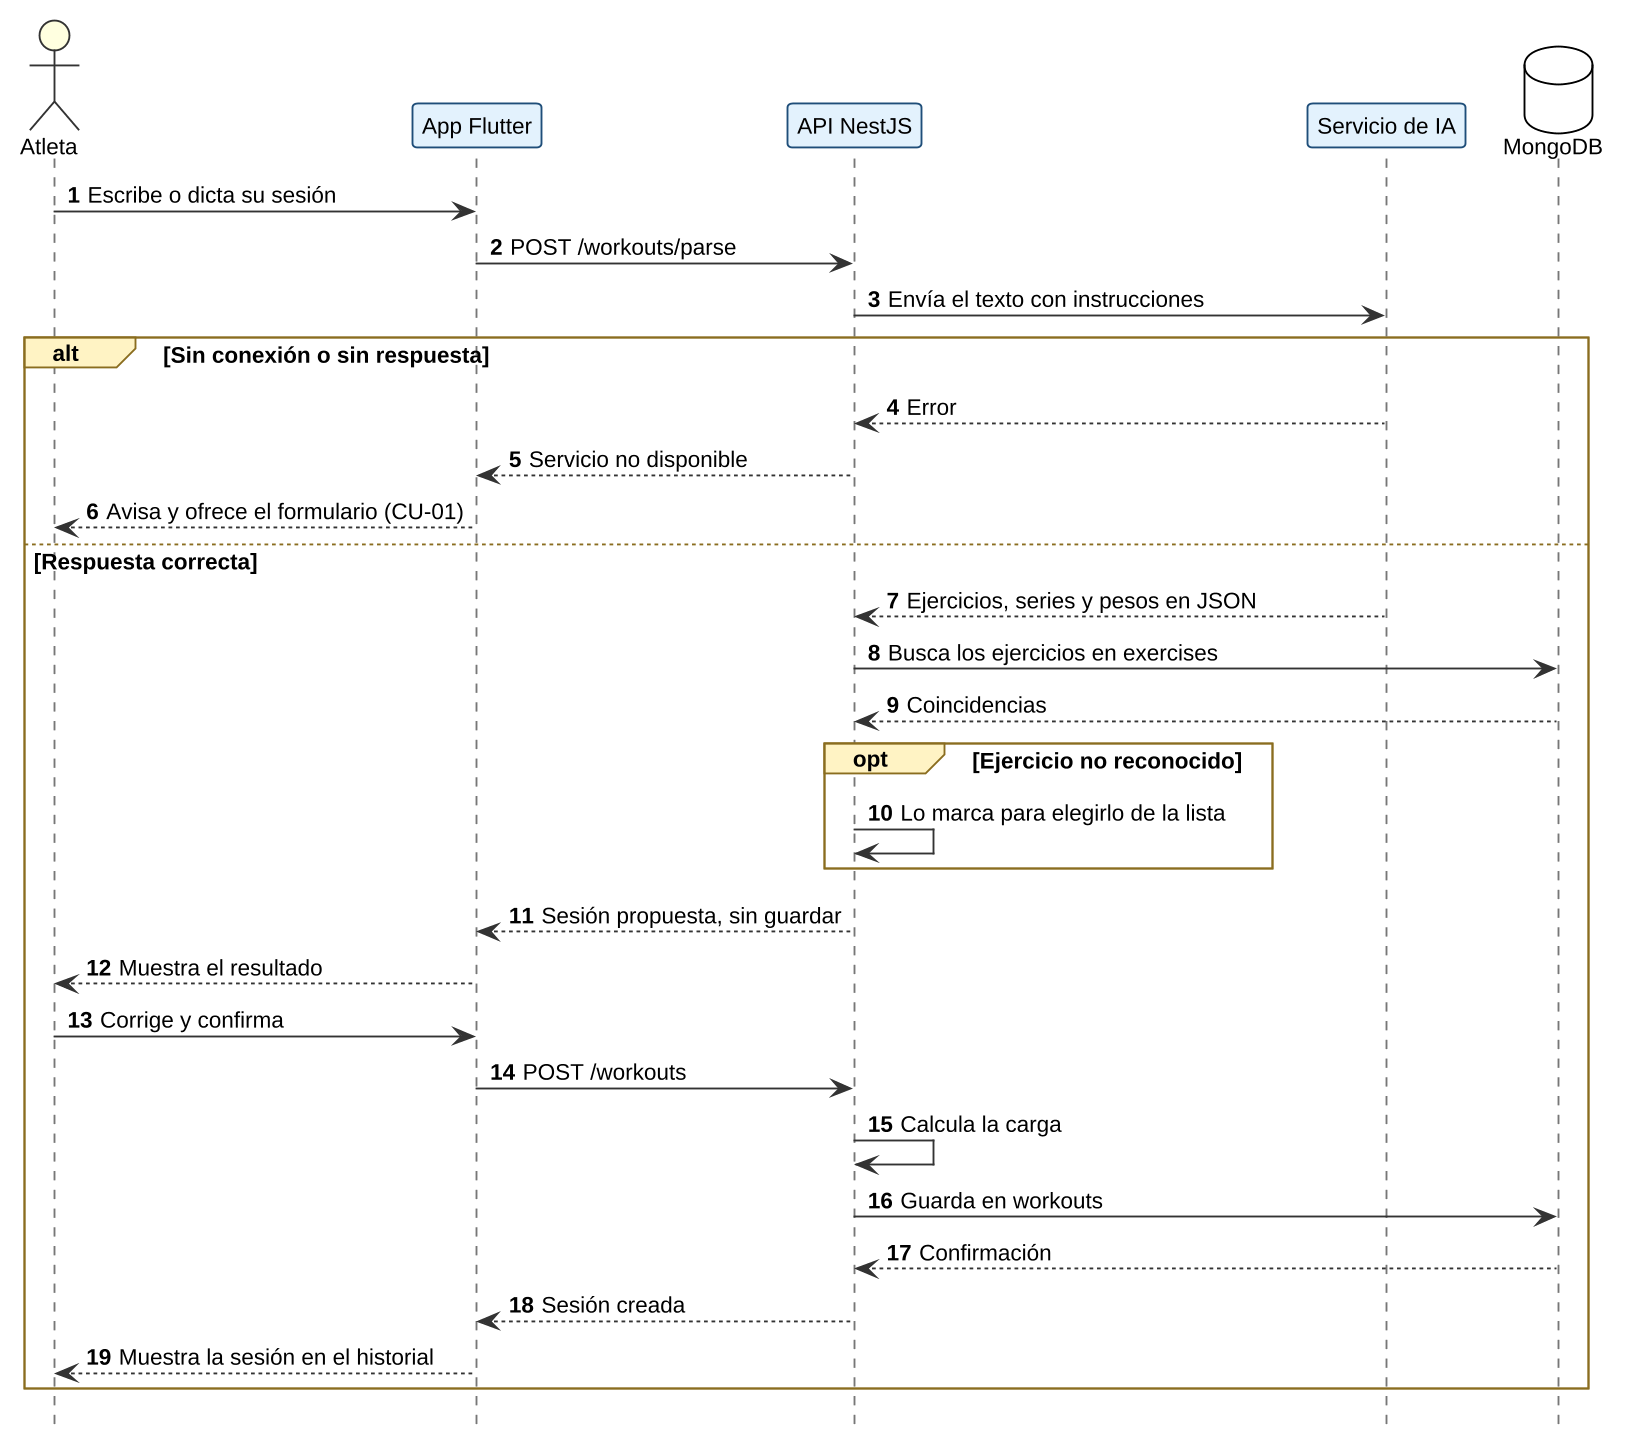
\includegraphics[width=0.95\textwidth,height=0.6\textheight,keepaspectratio]{figuras/secuencia/sec_cu02.png}
    \captionof{figure}{Diagrama de Secuencia -- CU-02: Contar mi sesión de fuerza con mis palabras.}
    \label{fig:sec_cu02}
\end{center}
La aplicación envía el texto al backend, y este lo reenvía al servicio de IA con instrucciones predefinidas para recibir la sesión ordenada en JSON. Luego compara cada ejercicio con el catálogo. La sesión solo se guarda cuando el usuario la confirma. Si el servicio de IA falla, se ofrece el formulario del CU-01.
\end{minipage}
\vspace{0.6cm}

\noindent\begin{minipage}{\linewidth}
\textbf{CU-03. Traer mis sesiones desde el reloj}

Para el caso de uso CU-03 se genera el diagrama de secuencia que se muestra en la Figura \ref{fig:sec_cu03}.
\begin{center}
    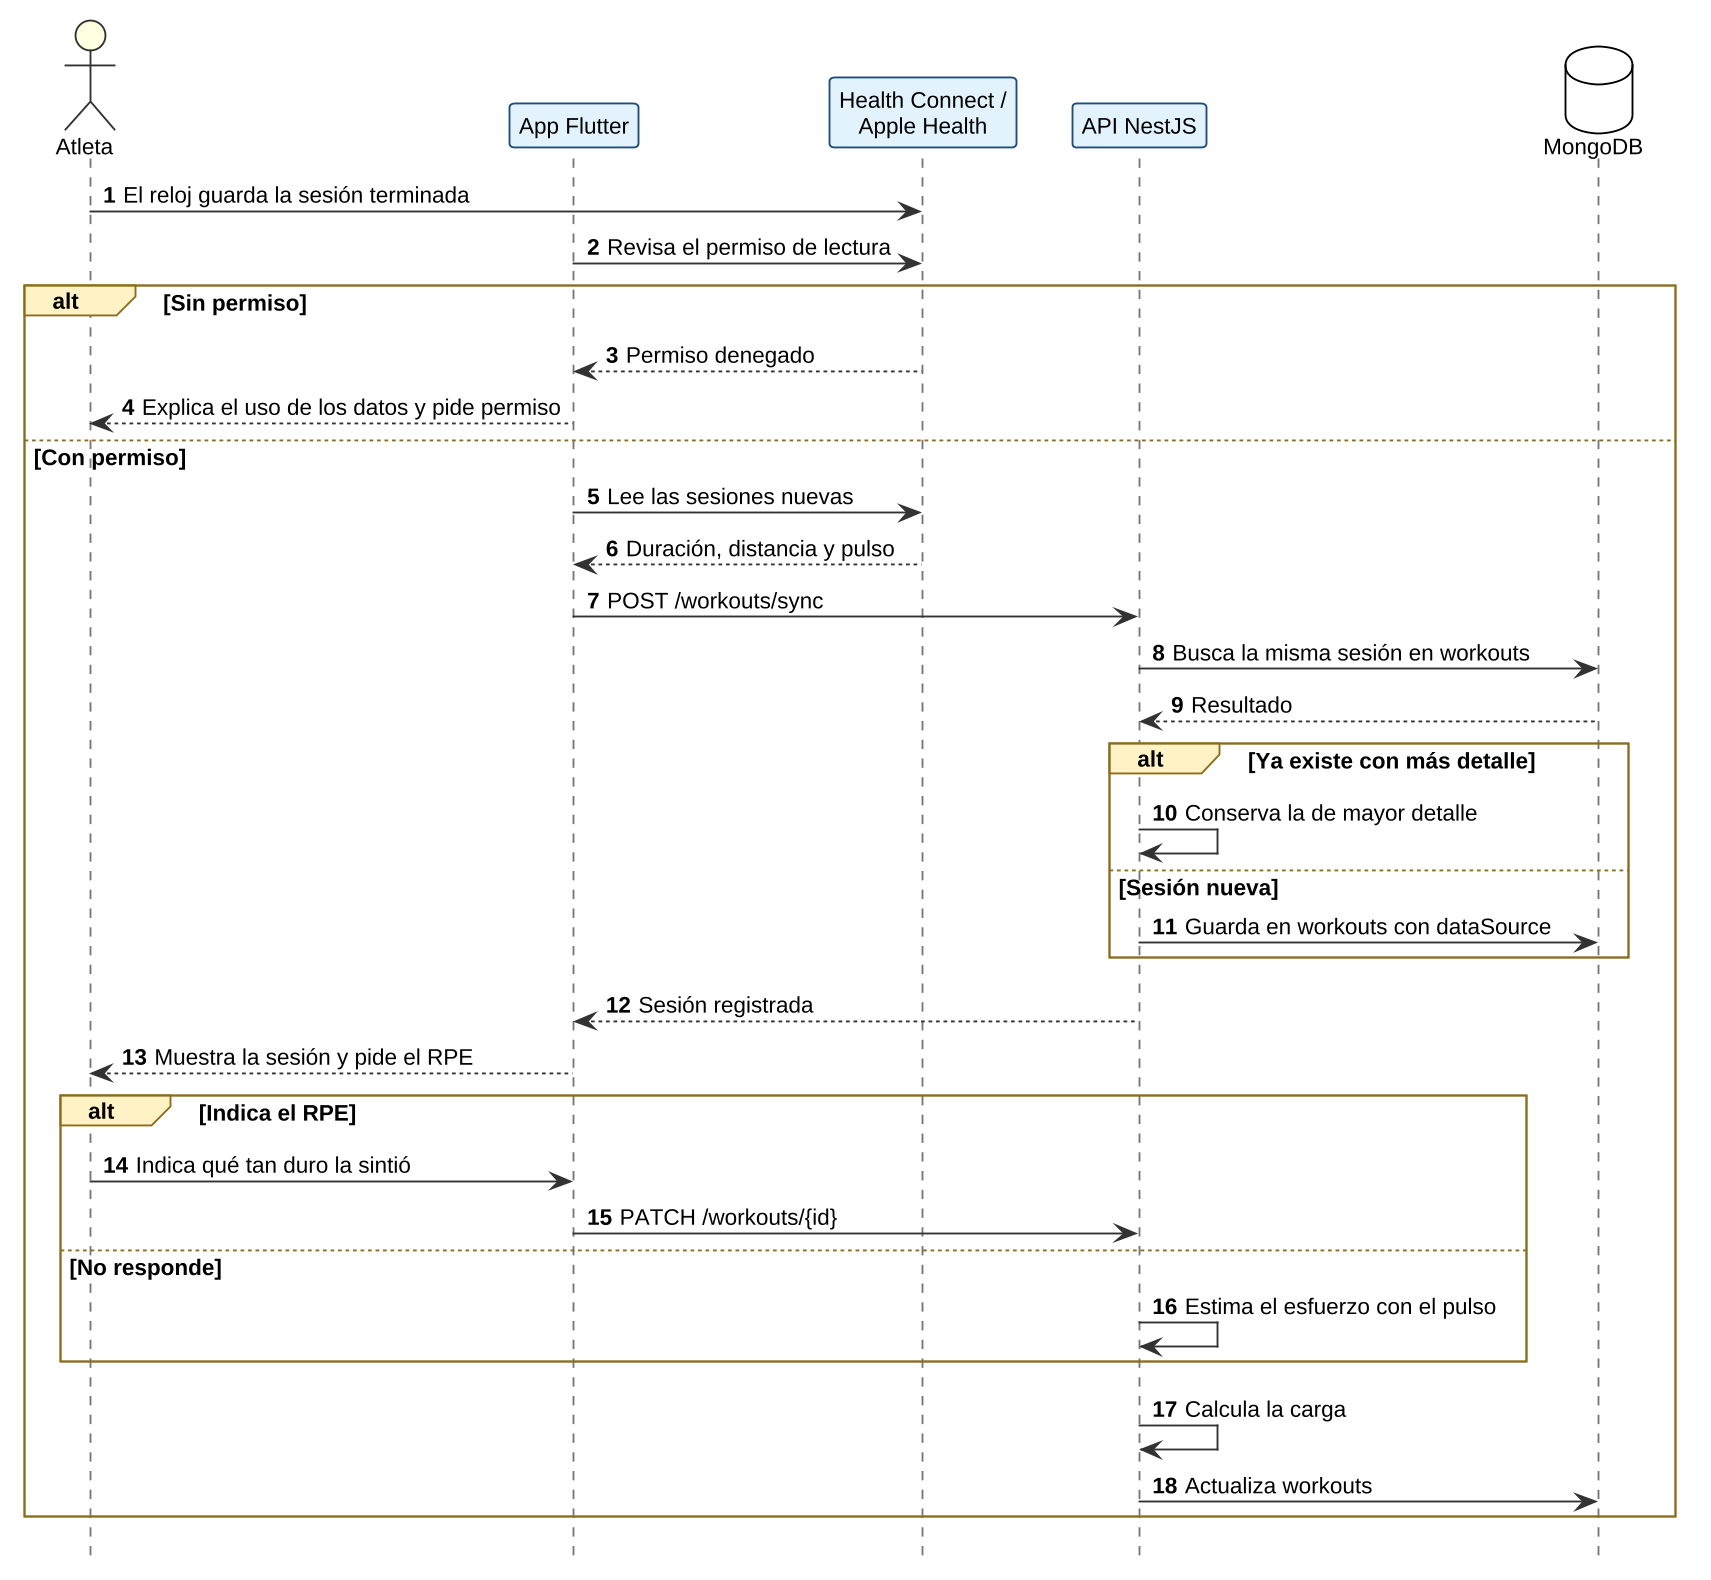
\includegraphics[width=0.95\textwidth,height=0.6\textheight,keepaspectratio]{figuras/secuencia/sec_cu03.png}
    \captionof{figure}{Diagrama de Secuencia -- CU-03: Traer mis sesiones desde el reloj.}
    \label{fig:sec_cu03}
\end{center}
La lectura la hace la aplicación en el teléfono, porque Health Connect y Apple Health no están disponibles desde el servidor. Con el permiso del usuario, lee las sesiones nuevas y las envía al backend. Este revisa que la misma sesión no exista ya con más detalle y luego la guarda. Si el usuario no indica su RPE, el esfuerzo se estima con el pulso.
\end{minipage}
\vspace{0.6cm}

\noindent\begin{minipage}{\linewidth}
\textbf{CU-04. Subir el archivo de mi ciclocomputador}

Para el caso de uso CU-04 se genera el diagrama de secuencia que se muestra en la Figura \ref{fig:sec_cu04}.
\begin{center}
    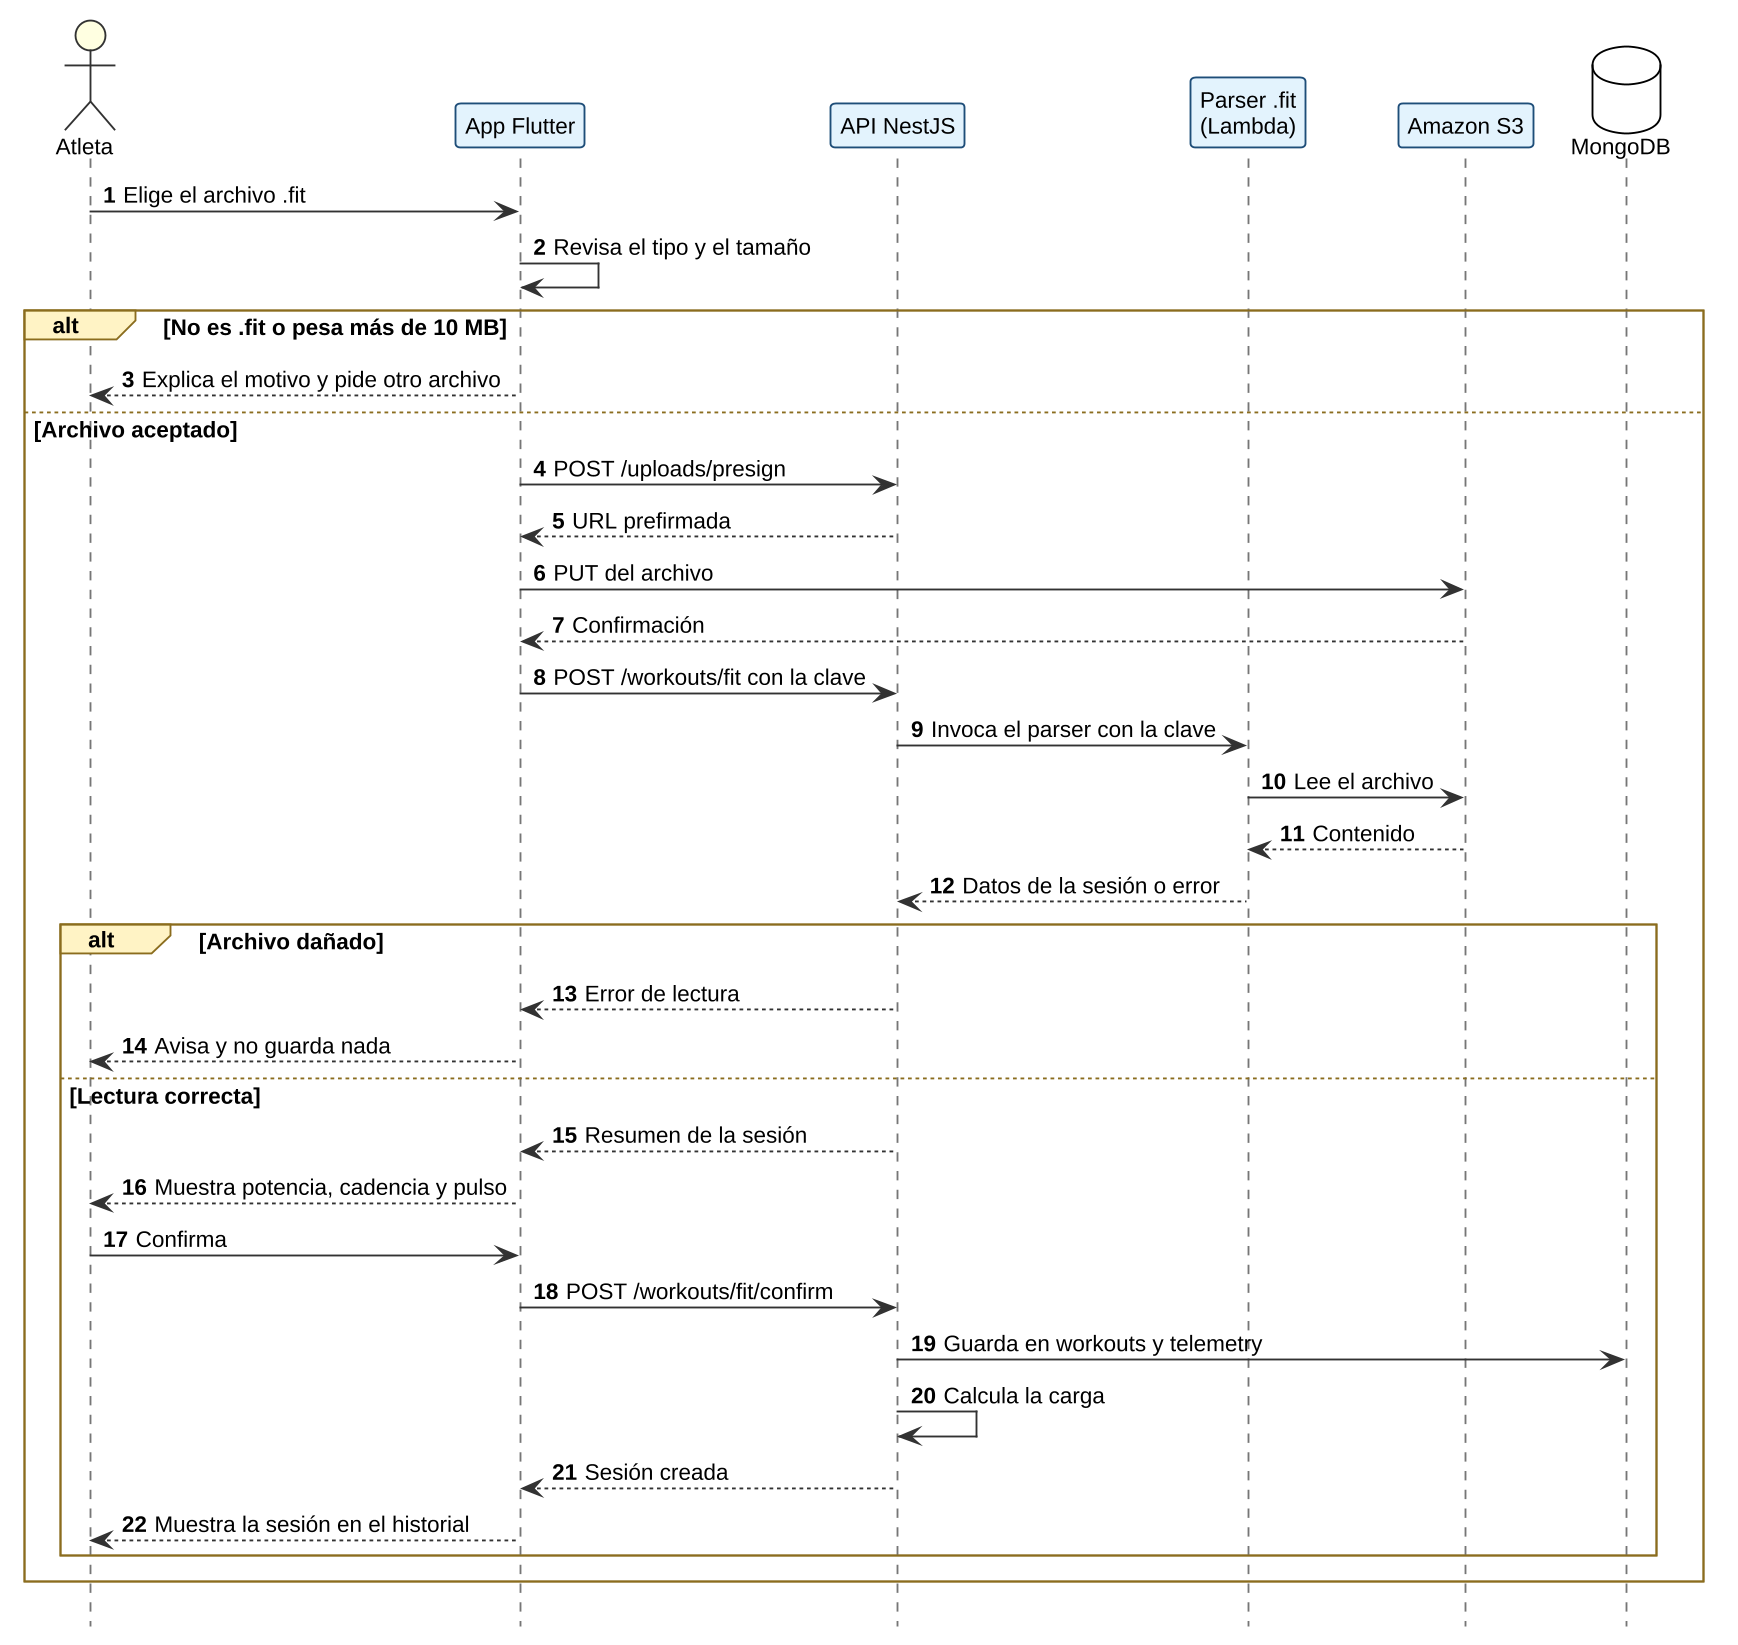
\includegraphics[width=0.95\textwidth,height=0.6\textheight,keepaspectratio]{figuras/secuencia/sec_cu04.png}
    \captionof{figure}{Diagrama de Secuencia -- CU-04: Subir el archivo de mi ciclocomputador.}
    \label{fig:sec_cu04}
\end{center}
El archivo se sube directamente a Amazon S3 con una URL prefirmada, para que el backend no reciba archivos pesados. Luego el backend invoca una función Lambda, que lee el archivo con el parser y devuelve un resumen. Al confirmar el usuario, guarda la sesión en \texttt{workouts} y los datos segundo a segundo en \texttt{telemetry}. Si el archivo está dañado no se guarda ningún dato, y el archivo en S3 se borra con la regla automática del bucket.
\end{minipage}
\vspace{0.6cm}

\noindent\begin{minipage}{\linewidth}
\textbf{CU-05. Revisar mi fatiga y recibir alertas}

Para el caso de uso CU-05 se genera el diagrama de secuencia que se muestra en la Figura \ref{fig:sec_cu05}.
\begin{center}
    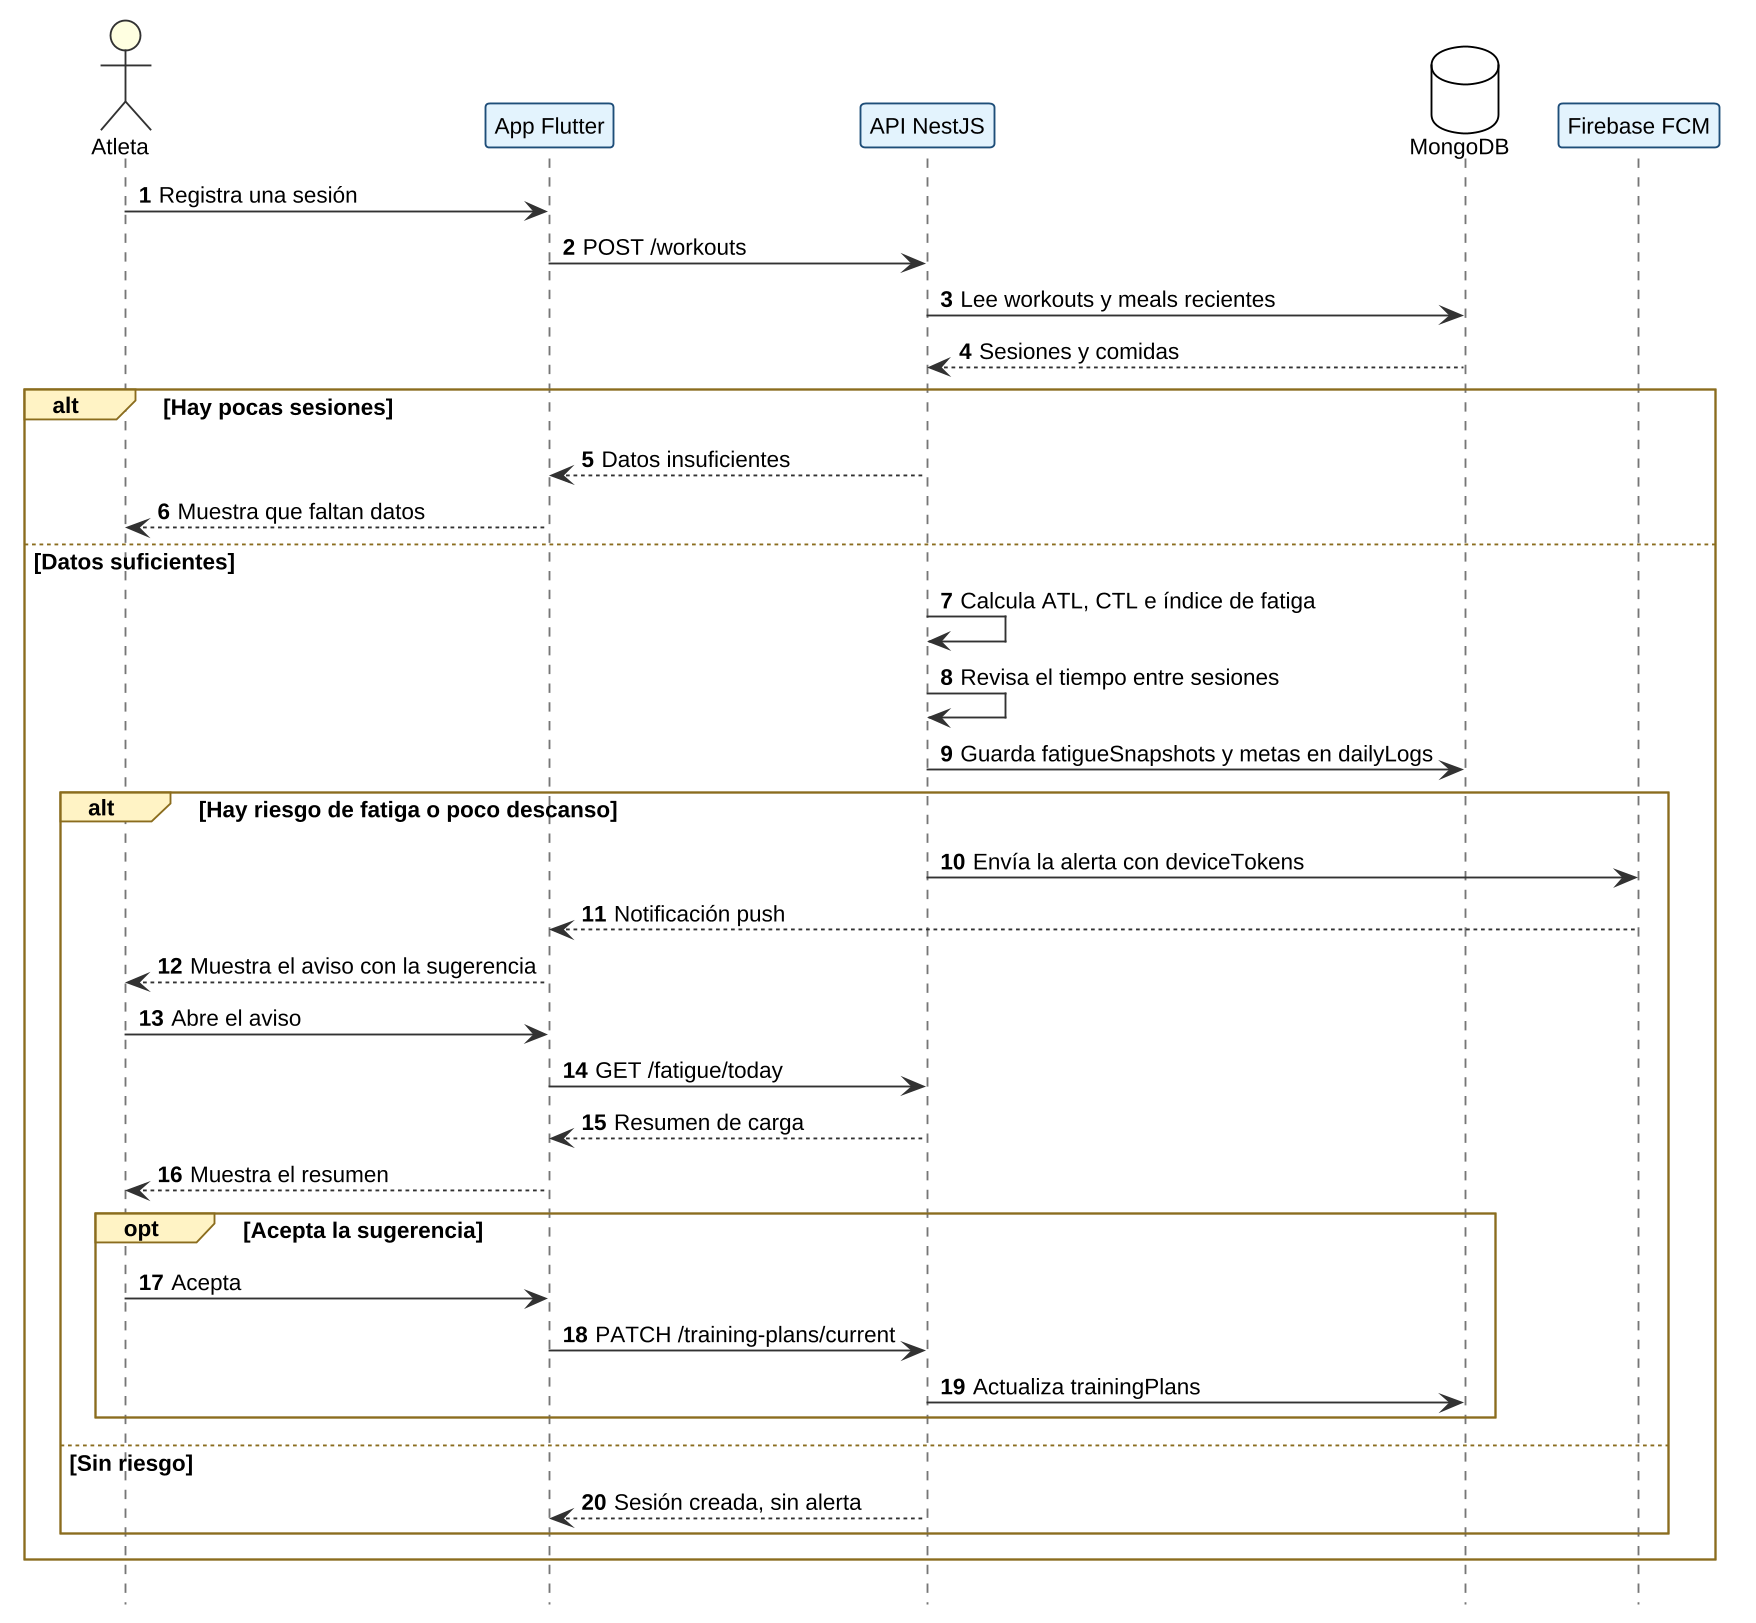
\includegraphics[width=0.95\textwidth,height=0.6\textheight,keepaspectratio]{figuras/secuencia/sec_cu05.png}
    \captionof{figure}{Diagrama de Secuencia -- CU-05: Revisar mi fatiga y recibir alertas.}
    \label{fig:sec_cu05}
\end{center}
El cálculo se hace después de cada sesión. El backend lee las sesiones y comidas recientes, calcula las cargas ATL y CTL, el índice de fatiga y el tiempo entre sesiones, y guarda el resultado en \texttt{fatigueSnapshots}. También actualiza las metas del día. Si detecta un riesgo, envía la alerta por Firebase Cloud Messaging. El plan solo cambia si el usuario acepta la sugerencia.
\end{minipage}
\vspace{0.6cm}

\noindent\begin{minipage}{\linewidth}
\textbf{CU-06. Anotar una comida buscando los alimentos}

Para el caso de uso CU-06 se genera el diagrama de secuencia que se muestra en la Figura \ref{fig:sec_cu06}.
\begin{center}
    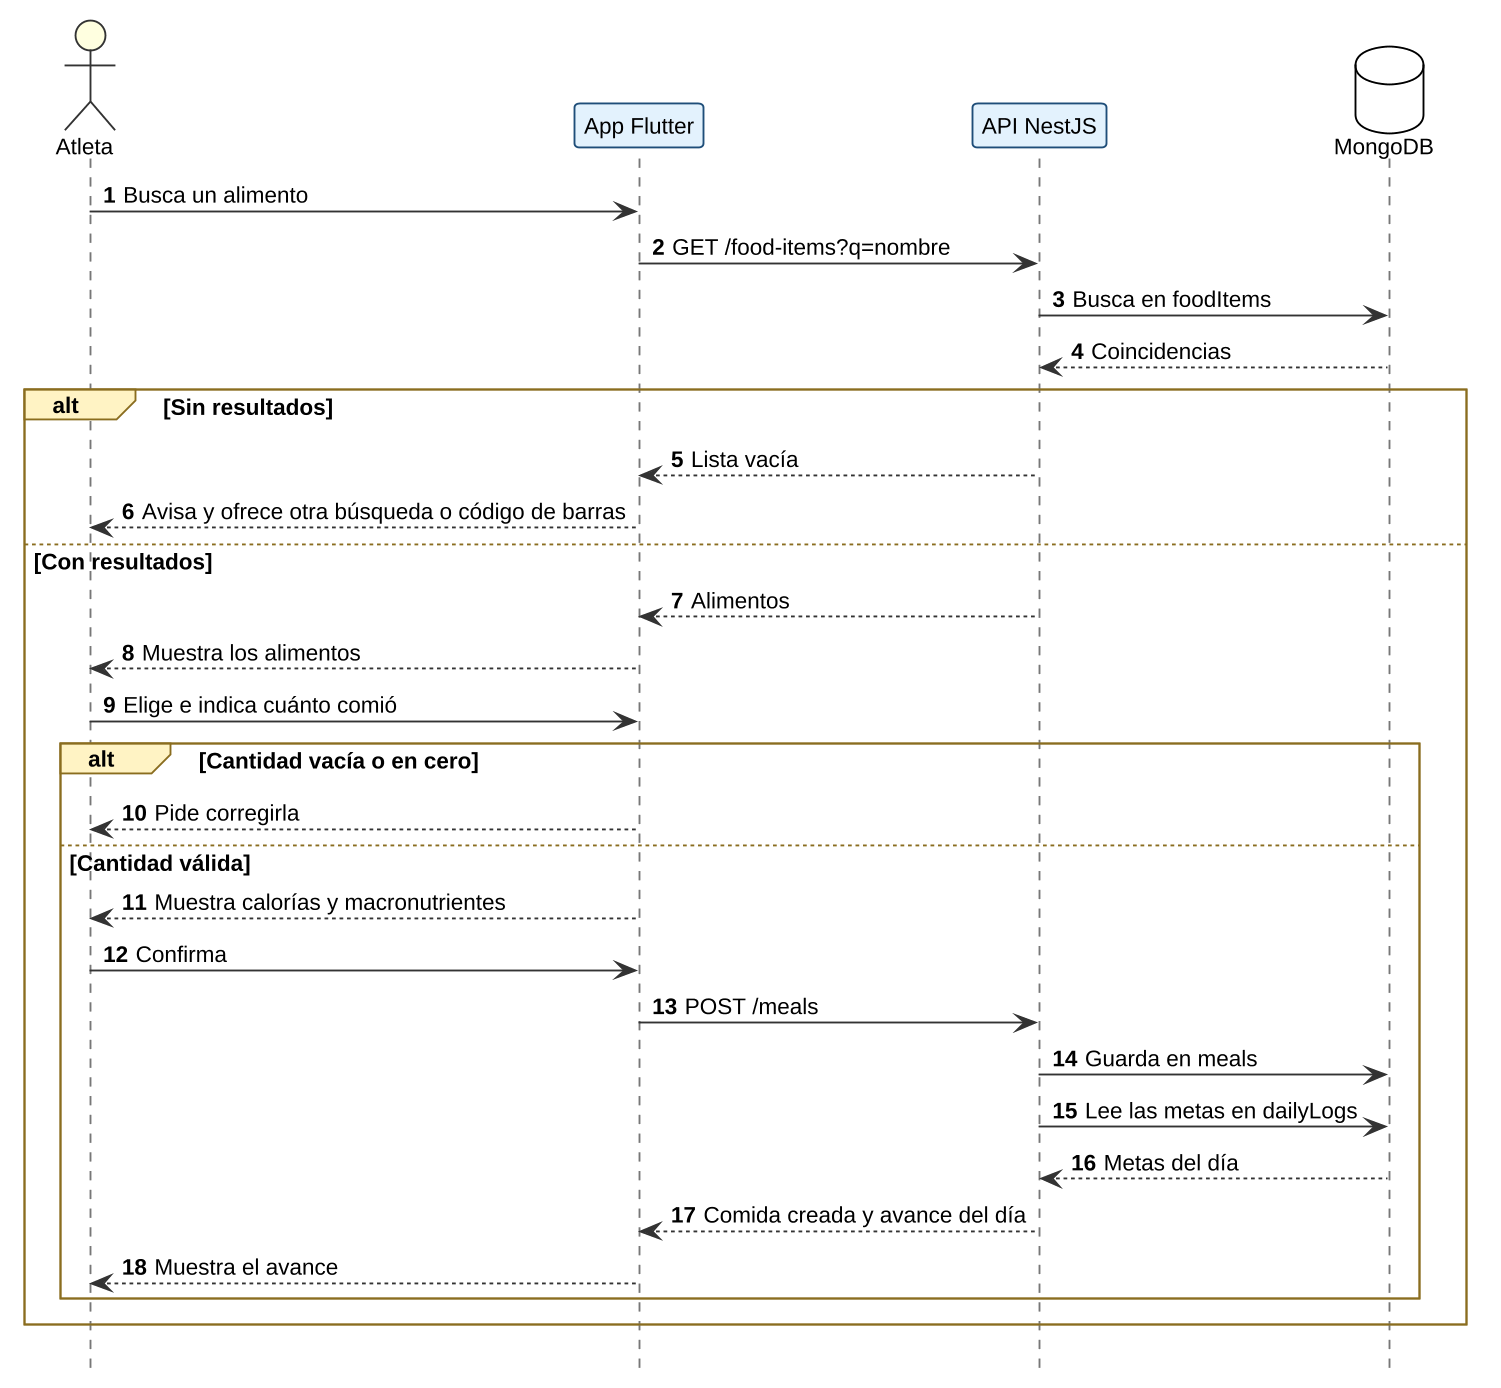
\includegraphics[width=0.95\textwidth,height=0.6\textheight,keepaspectratio]{figuras/secuencia/sec_cu06.png}
    \captionof{figure}{Diagrama de Secuencia -- CU-06: Anotar una comida buscando los alimentos.}
    \label{fig:sec_cu06}
\end{center}
La aplicación busca en el catálogo \texttt{foodItems} a través del backend. Una vez elegido el alimento, revisa la cantidad, muestra los valores y envía la comida. El backend la guarda en \texttt{meals} y responde con el avance respecto a las metas del día.
\end{minipage}
\vspace{0.6cm}

\noindent\begin{minipage}{\linewidth}
\textbf{CU-07. Registrar una comida con una foto}

Para el caso de uso CU-07 se genera el diagrama de secuencia que se muestra en la Figura \ref{fig:sec_cu07}.
\begin{center}
    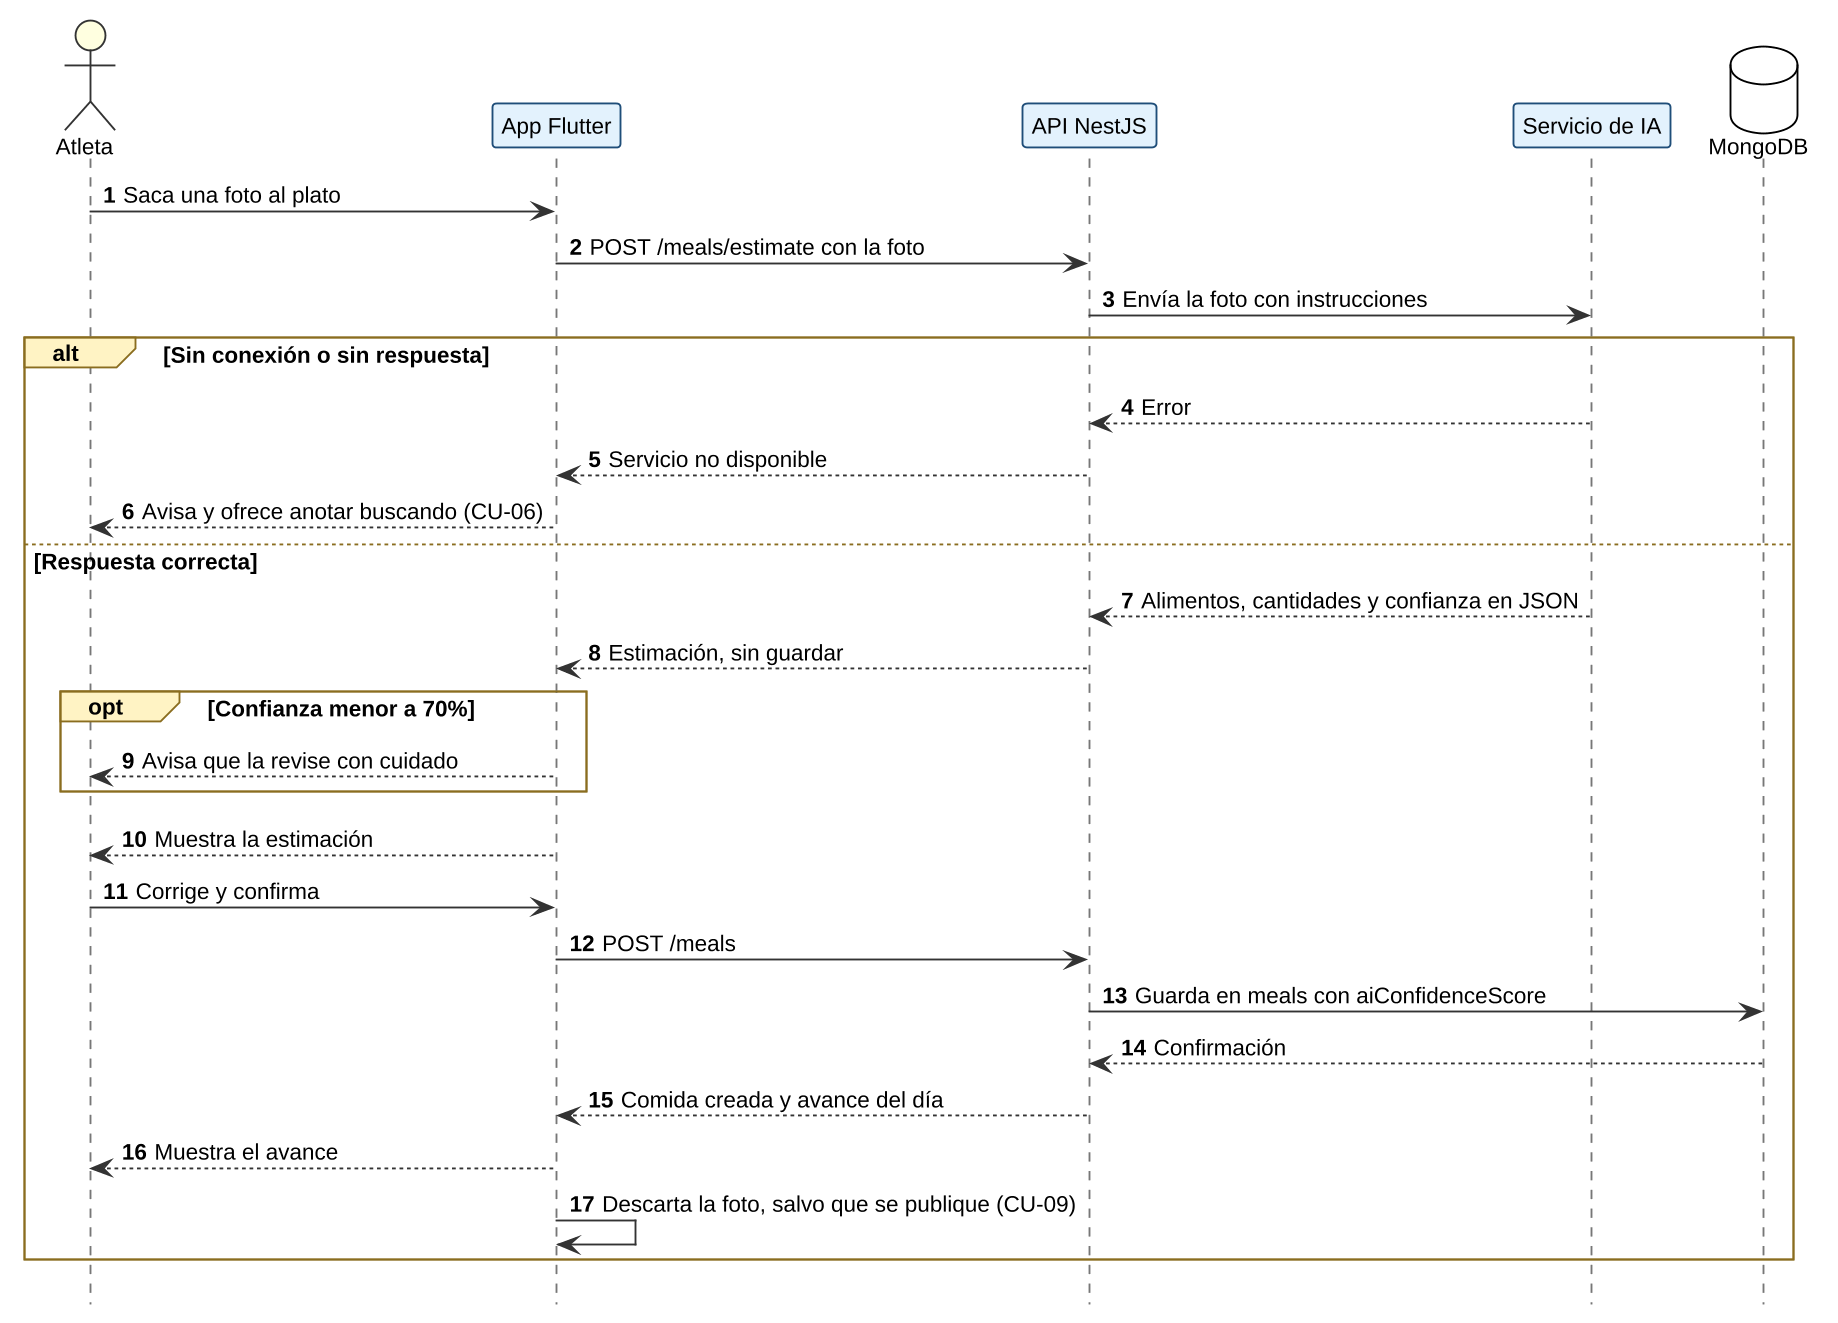
\includegraphics[width=0.95\textwidth,height=0.6\textheight,keepaspectratio]{figuras/secuencia/sec_cu07.png}
    \captionof{figure}{Diagrama de Secuencia -- CU-07: Registrar una comida con una foto.}
    \label{fig:sec_cu07}
\end{center}
La foto se envía al backend y este la reenvía al servicio de IA, sin guardarla en Amazon S3. La respuesta incluye un índice de confianza, y si es menor a 70\% la aplicación pide revisar el resultado con más cuidado. La comida se guarda solo cuando el usuario confirma, junto con ese índice, y la foto se descarta salvo que se publique.
\end{minipage}
\vspace{0.6cm}

\noindent\begin{minipage}{\linewidth}
\textbf{CU-08. Agregar una receta ajustada a mis metas}

Para el caso de uso CU-08 se genera el diagrama de secuencia que se muestra en la Figura \ref{fig:sec_cu08}.
\begin{center}
    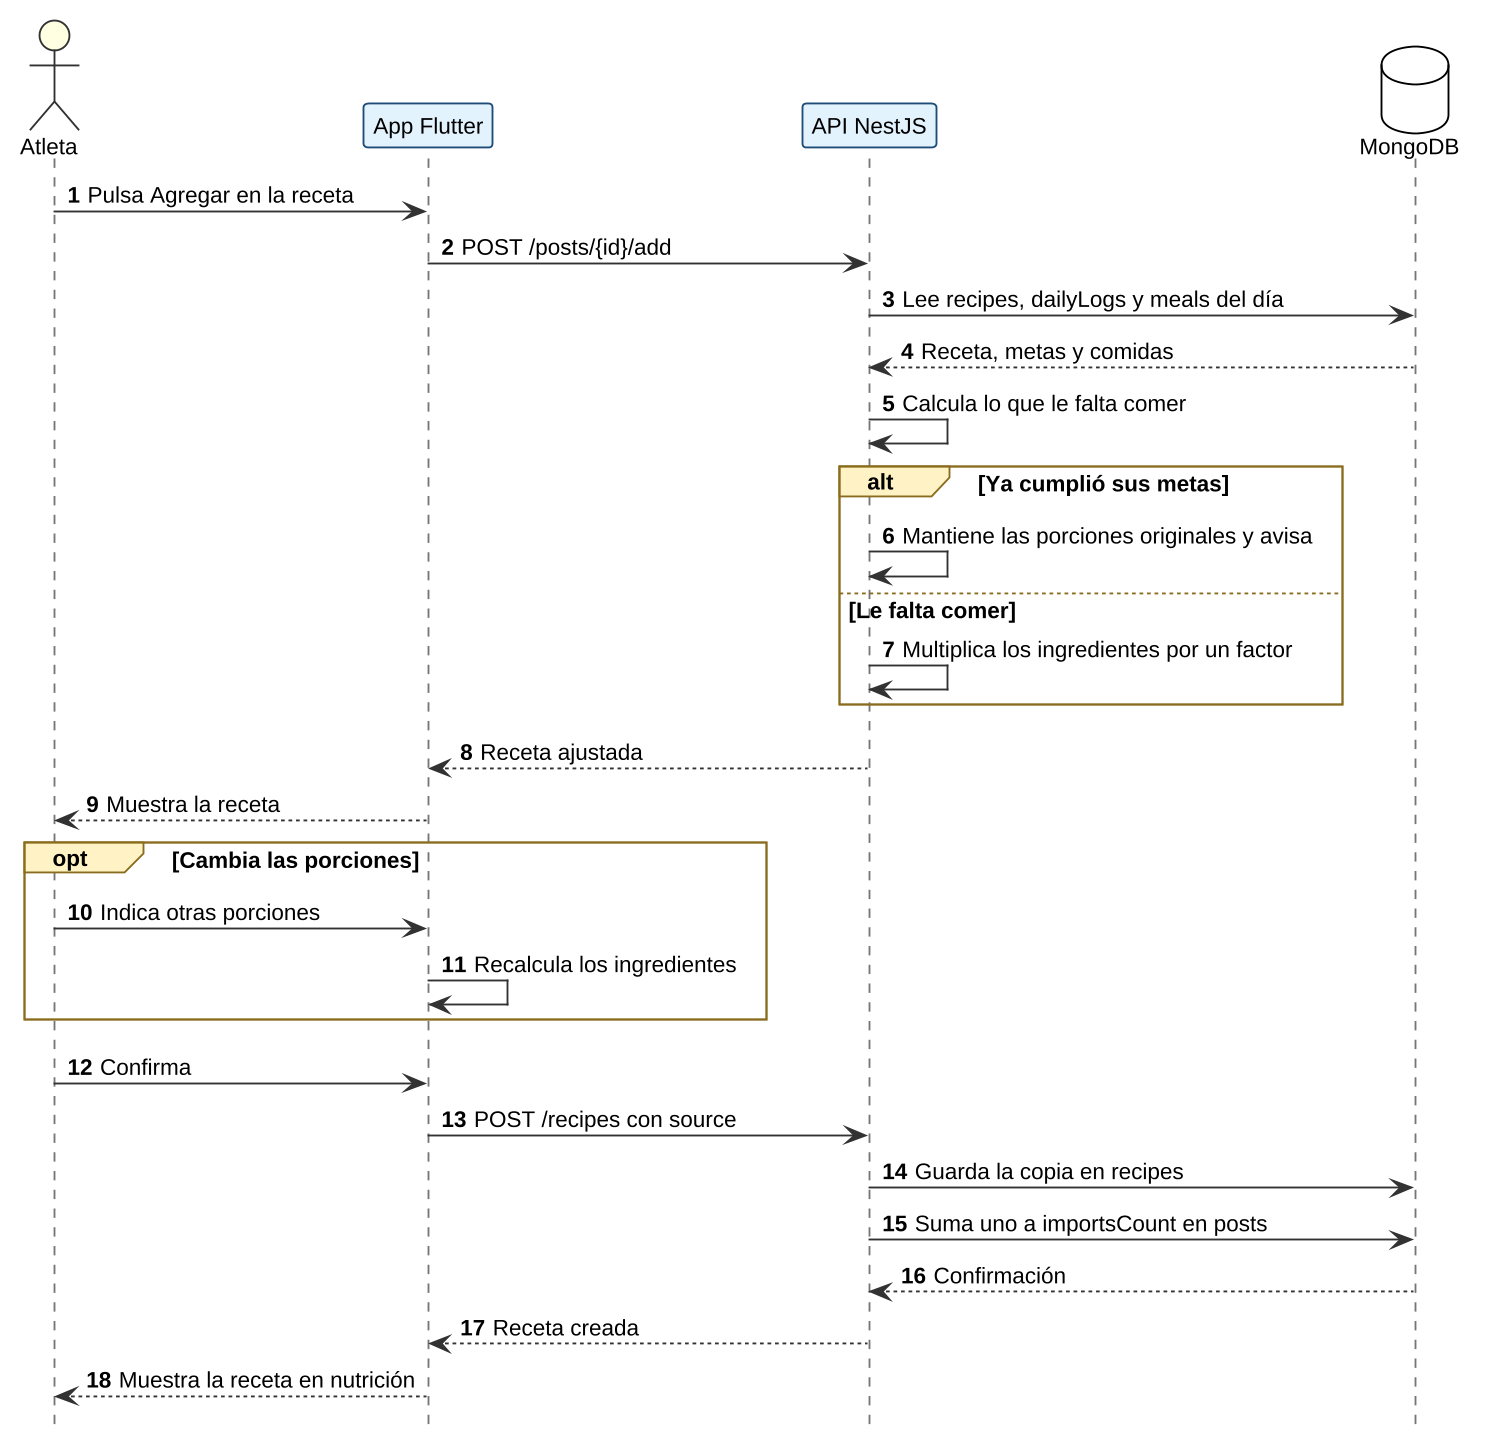
\includegraphics[width=0.95\textwidth,height=0.6\textheight,keepaspectratio]{figuras/secuencia/sec_cu08.png}
    \captionof{figure}{Diagrama de Secuencia -- CU-08: Agregar una receta ajustada a mis metas.}
    \label{fig:sec_cu08}
\end{center}
El backend lee la receta, las metas y las comidas del día para calcular lo que le falta comer al usuario. Con eso obtiene un factor y multiplica todos los ingredientes por él, de modo que las proporciones no cambian. Al confirmar, guarda una copia en \texttt{recipes} con la referencia a su autor y suma uno a \texttt{importsCount}. Agregar la receta no la registra como comida.
\end{minipage}
\vspace{0.6cm}

\noindent\begin{minipage}{\linewidth}
\textbf{CU-09. Publicar una sesión, ruta o comida}

Para el caso de uso CU-09 se genera el diagrama de secuencia que se muestra en la Figura \ref{fig:sec_cu09}.
\begin{center}
    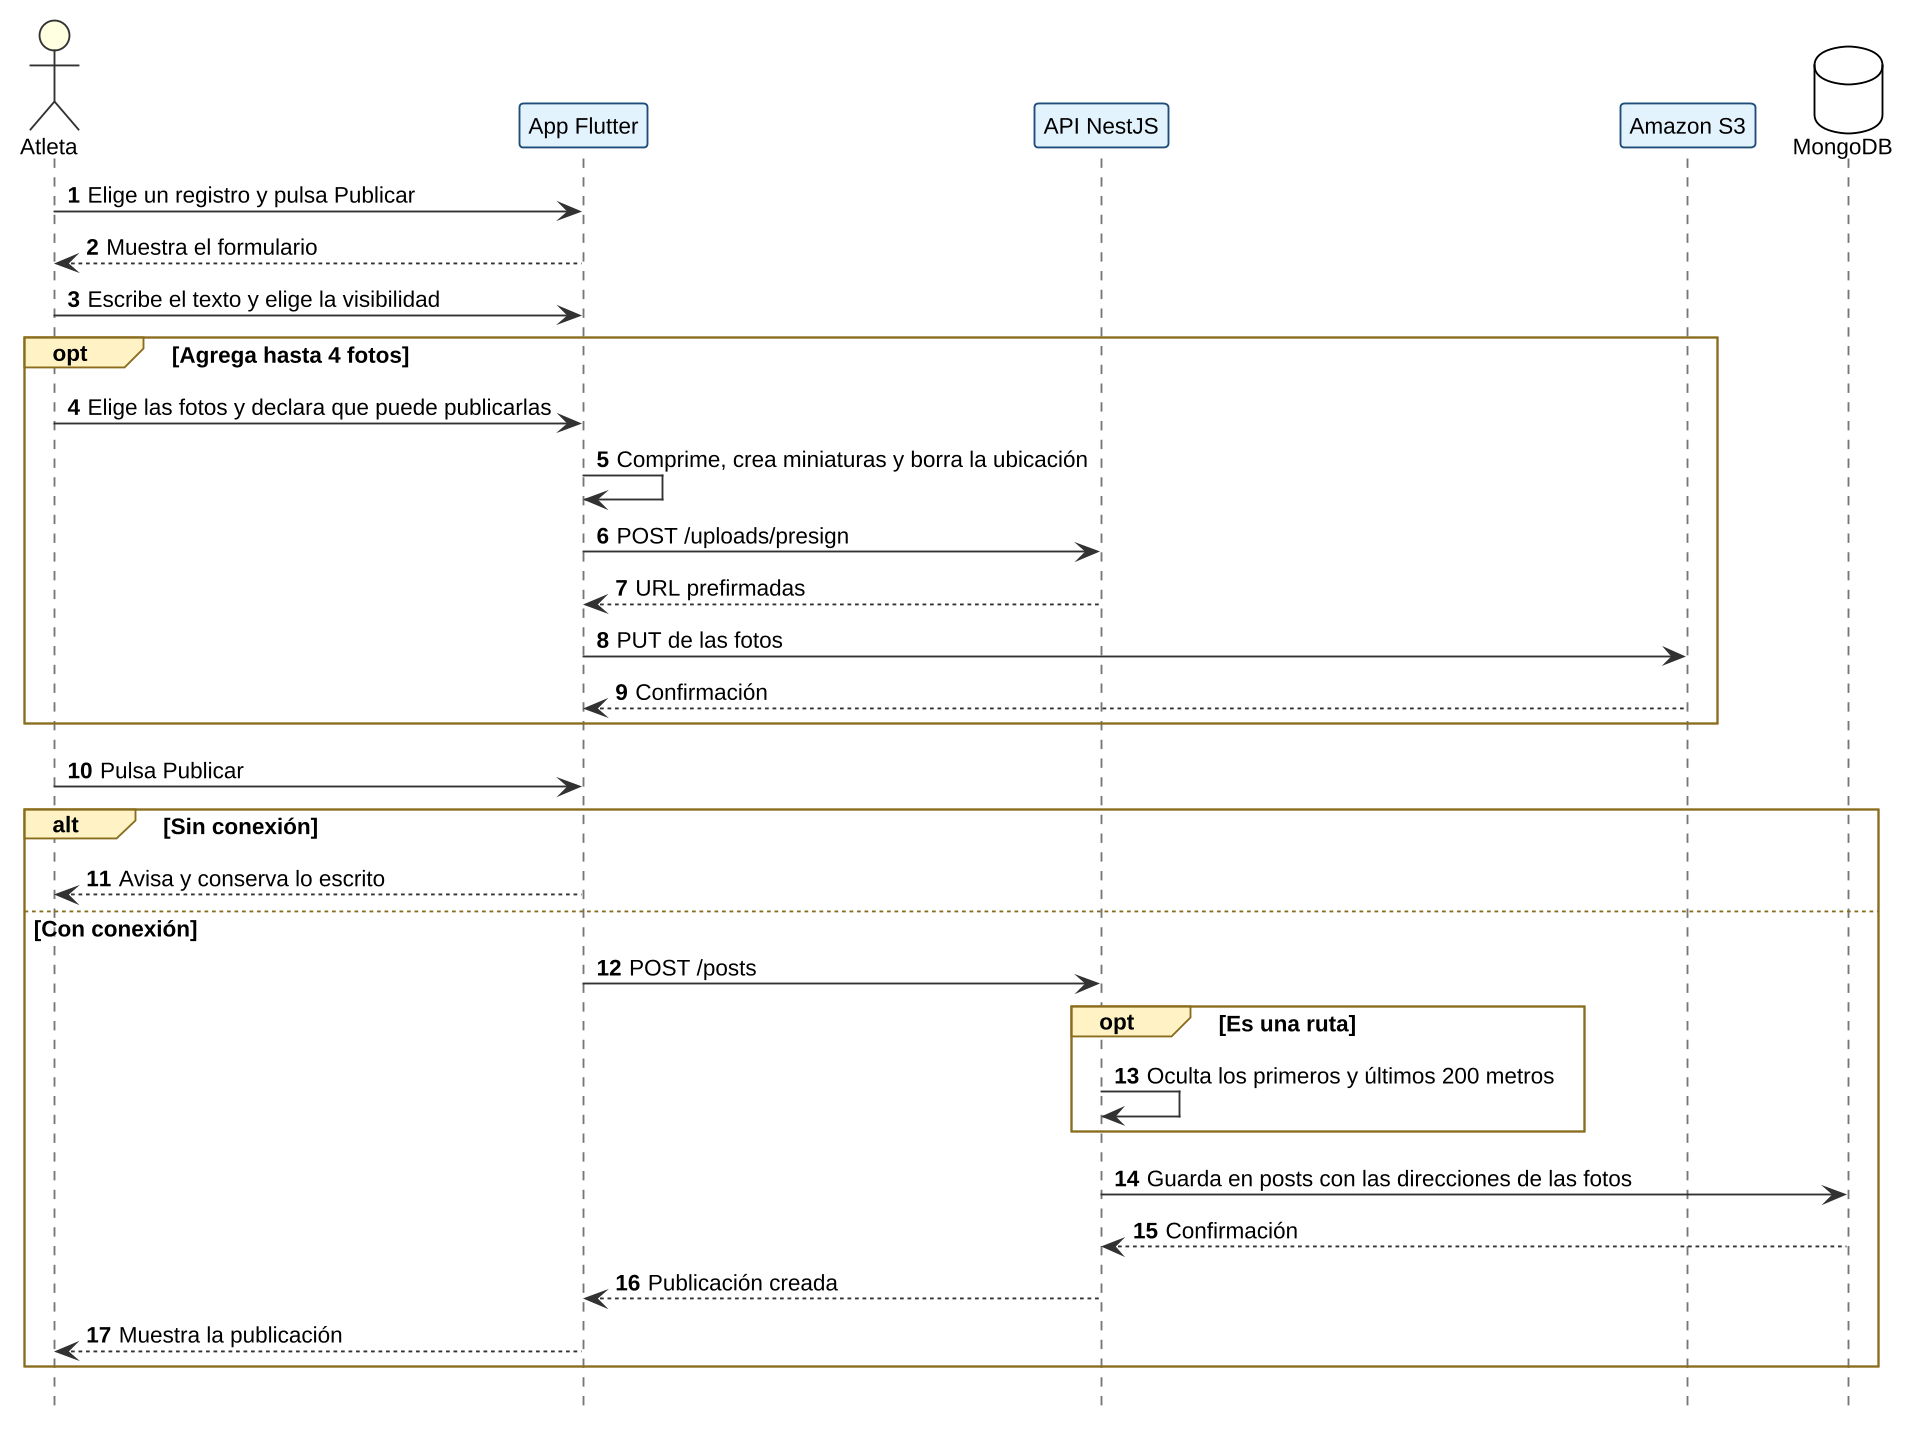
\includegraphics[width=0.95\textwidth,height=0.6\textheight,keepaspectratio]{figuras/secuencia/sec_cu09.png}
    \captionof{figure}{Diagrama de Secuencia -- CU-09: Publicar una sesión, ruta o comida.}
    \label{fig:sec_cu09}
\end{center}
Las fotos se comprimen en el teléfono, donde también se crean las miniaturas y se borra la ubicación. Después se suben directamente a Amazon S3 con URL prefirmadas. El backend guarda la publicación en \texttt{posts} solo con las direcciones de las fotos. Si es una ruta, oculta los primeros y los últimos 200 metros antes de guardarla.
\end{minipage}
\vspace{0.6cm}

\noindent\begin{minipage}{\linewidth}
\textbf{CU-10. Mantener el catálogo de ejercicios}

Para el caso de uso CU-10 se genera el diagrama de secuencia que se muestra en la Figura \ref{fig:sec_cu10}.
\begin{center}
    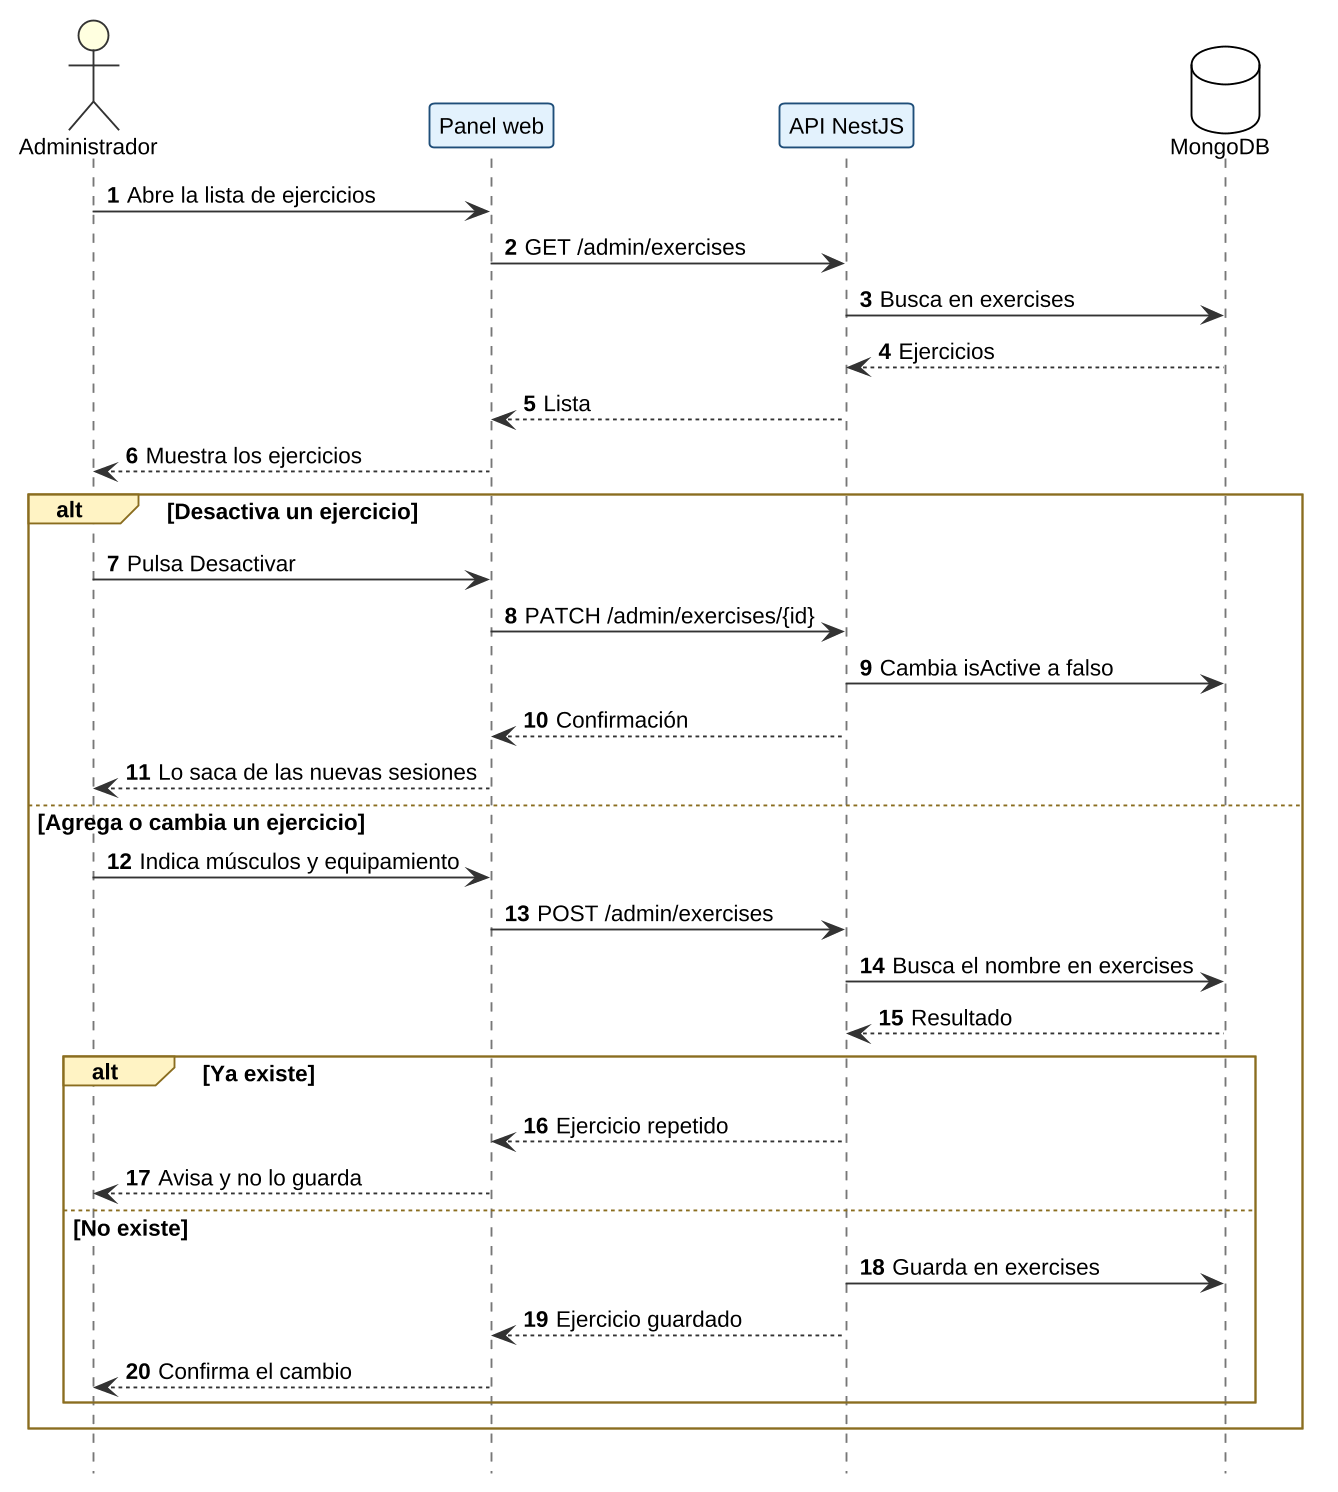
\includegraphics[width=0.95\textwidth,height=0.6\textheight,keepaspectratio]{figuras/secuencia/sec_cu10.png}
    \captionof{figure}{Diagrama de Secuencia -- CU-10: Mantener el catálogo de ejercicios.}
    \label{fig:sec_cu10}
\end{center}
El administrador trabaja desde el panel web, que usa el mismo backend con acceso solo para su rol. Antes de guardar un ejercicio, el backend revisa que el nombre no exista. Los ejercicios no se borran, sino que se desactivan con \texttt{isActive}, para no alterar las sesiones ya registradas.
\end{minipage}
\vspace{0.6cm}

\noindent\begin{minipage}{\linewidth}
\textbf{CU-11. Revisar el contenido reportado}

Para el caso de uso CU-11 se genera el diagrama de secuencia que se muestra en la Figura \ref{fig:sec_cu11}.
\begin{center}
    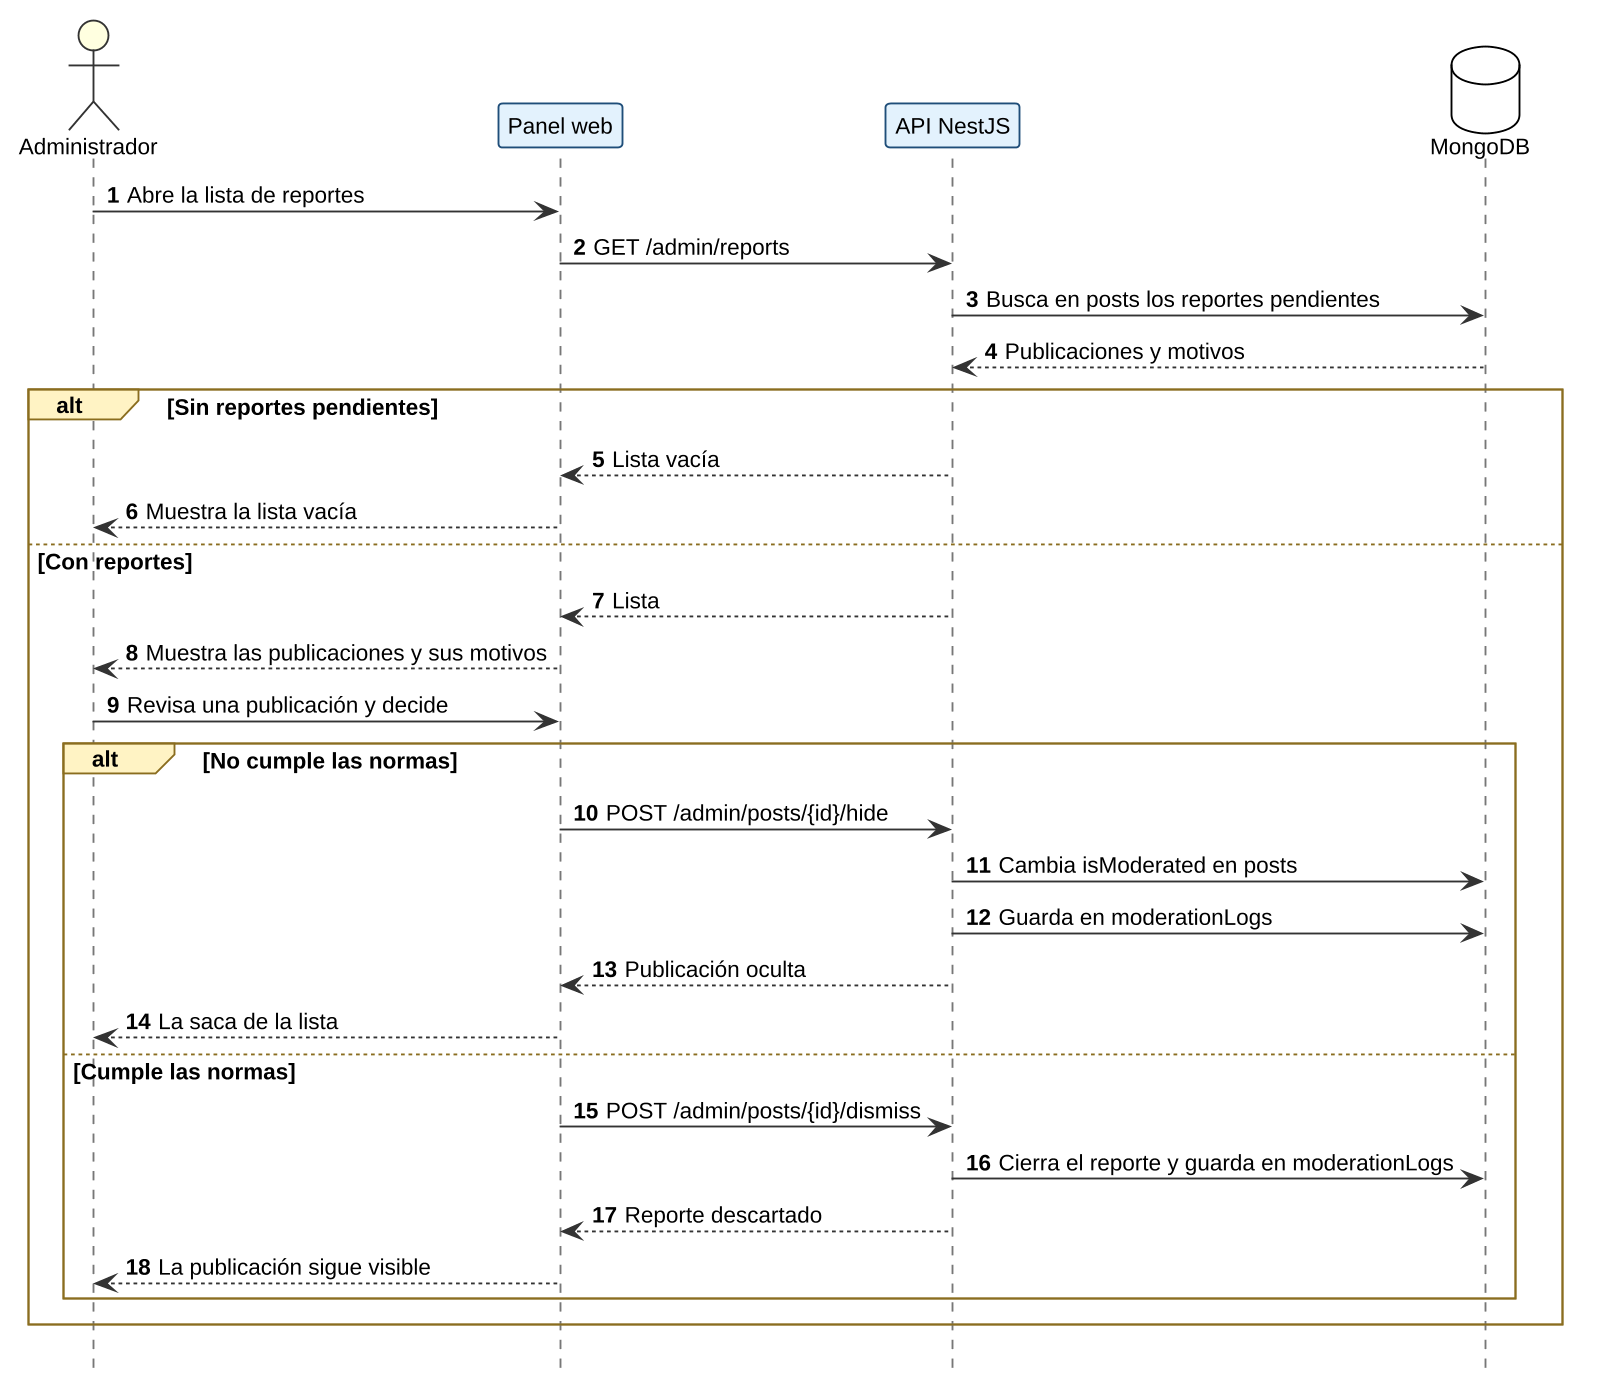
\includegraphics[width=0.95\textwidth,height=0.6\textheight,keepaspectratio]{figuras/secuencia/sec_cu11.png}
    \captionof{figure}{Diagrama de Secuencia -- CU-11: Revisar el contenido reportado.}
    \label{fig:sec_cu11}
\end{center}
El backend busca las publicaciones con reportes pendientes y las muestra con sus motivos. Si el administrador decide ocultar una publicación, esta sale del muro. Cualquiera sea la decisión, queda guardada en \texttt{moderationLogs} con quién la tomó y por qué.
\end{minipage}
\vspace{0.6cm}

\noindent\begin{minipage}{\linewidth}
\textbf{CU-12. Completar mi perfil y recibir un plan semanal}

Para el caso de uso CU-12 se genera el diagrama de secuencia que se muestra en la Figura \ref{fig:sec_cu12}.
\begin{center}
    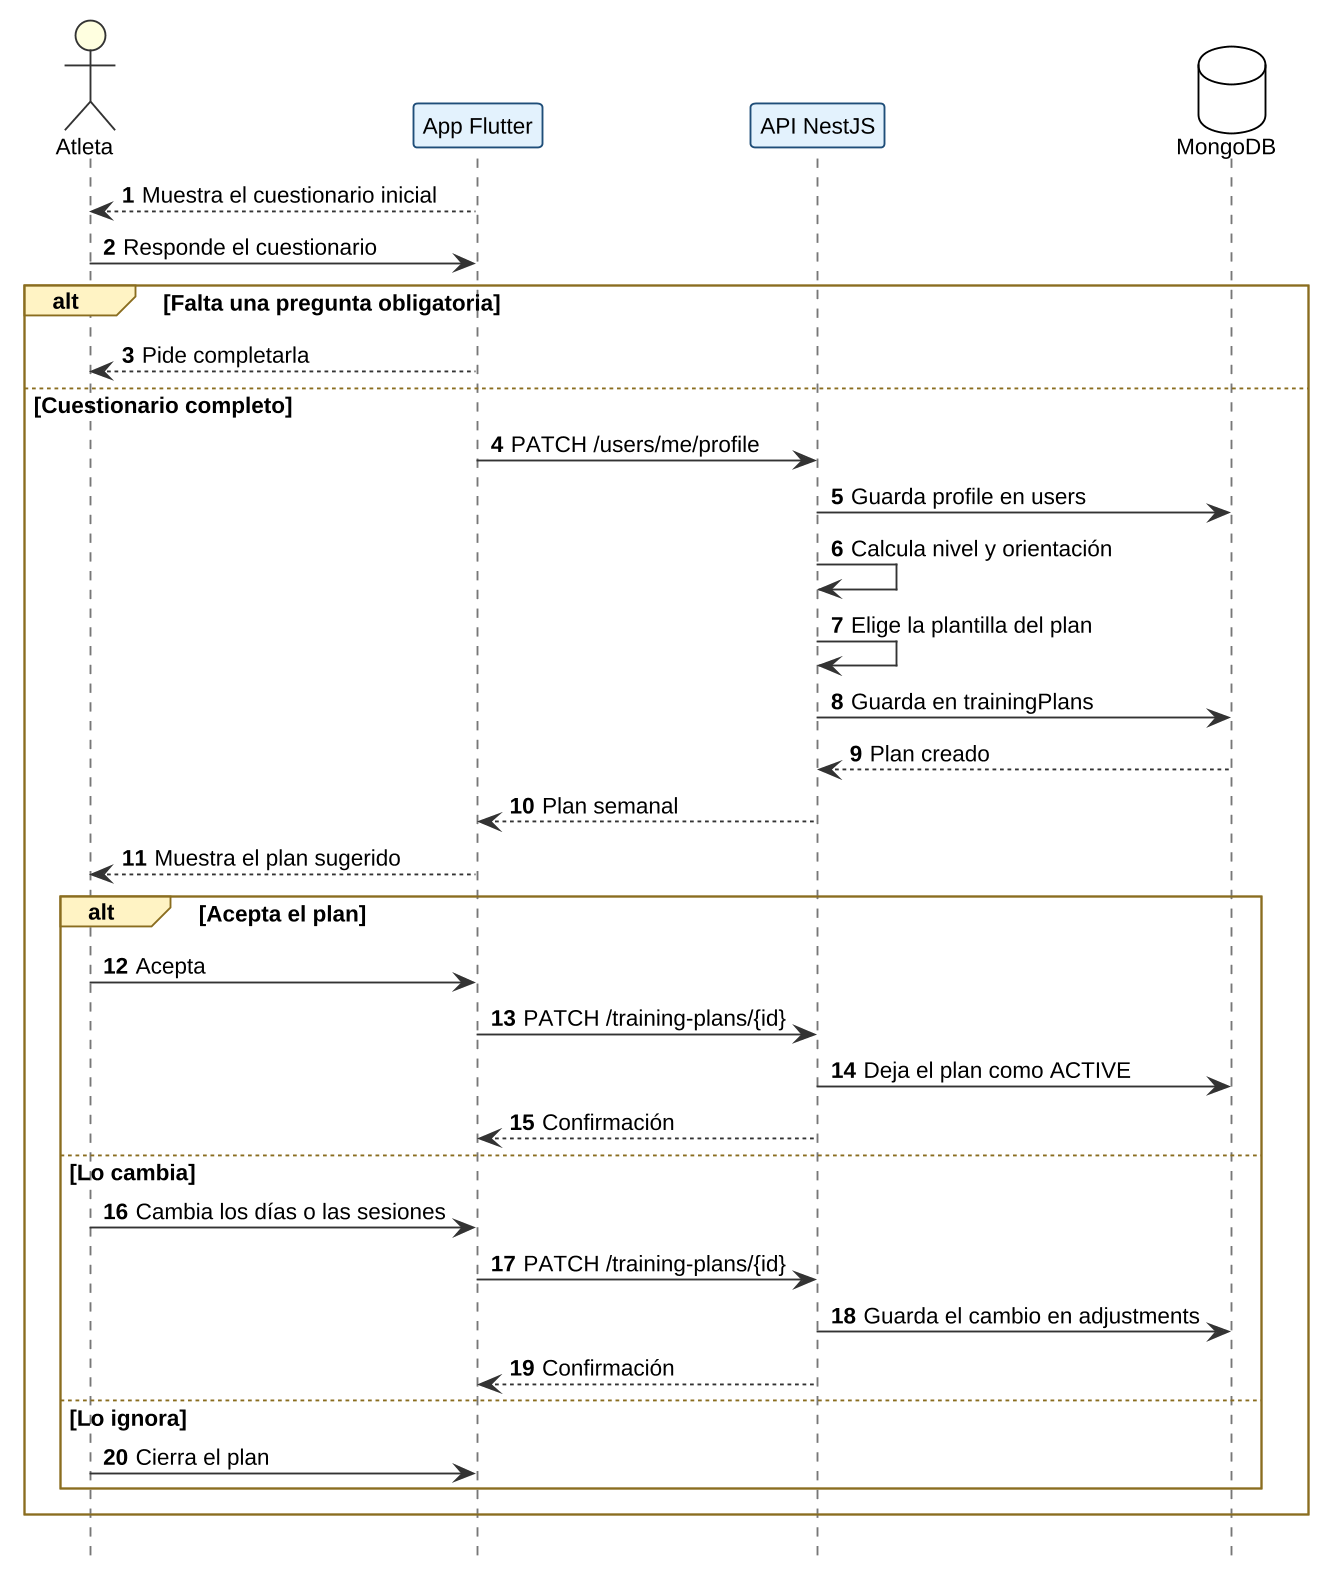
\includegraphics[width=0.95\textwidth,height=0.6\textheight,keepaspectratio]{figuras/secuencia/sec_cu12.png}
    \captionof{figure}{Diagrama de Secuencia -- CU-12: Completar mi perfil y recibir un plan semanal.}
    \label{fig:sec_cu12}
\end{center}
Con las respuestas del cuestionario, el backend actualiza el perfil, calcula el nivel y la orientación del usuario y elige la plantilla correspondiente, definida en el propio backend. El plan se guarda en \texttt{trainingPlans}. Si el usuario lo cambia, el cambio queda registrado en \texttt{adjustments}.
\end{minipage}
\vspace{0.6cm}

\noindent\begin{minipage}{\linewidth}
\textbf{CU-13. Agregar una publicación a mis módulos}

Para el caso de uso CU-13 se genera el diagrama de secuencia que se muestra en la Figura \ref{fig:sec_cu13}.
\begin{center}
    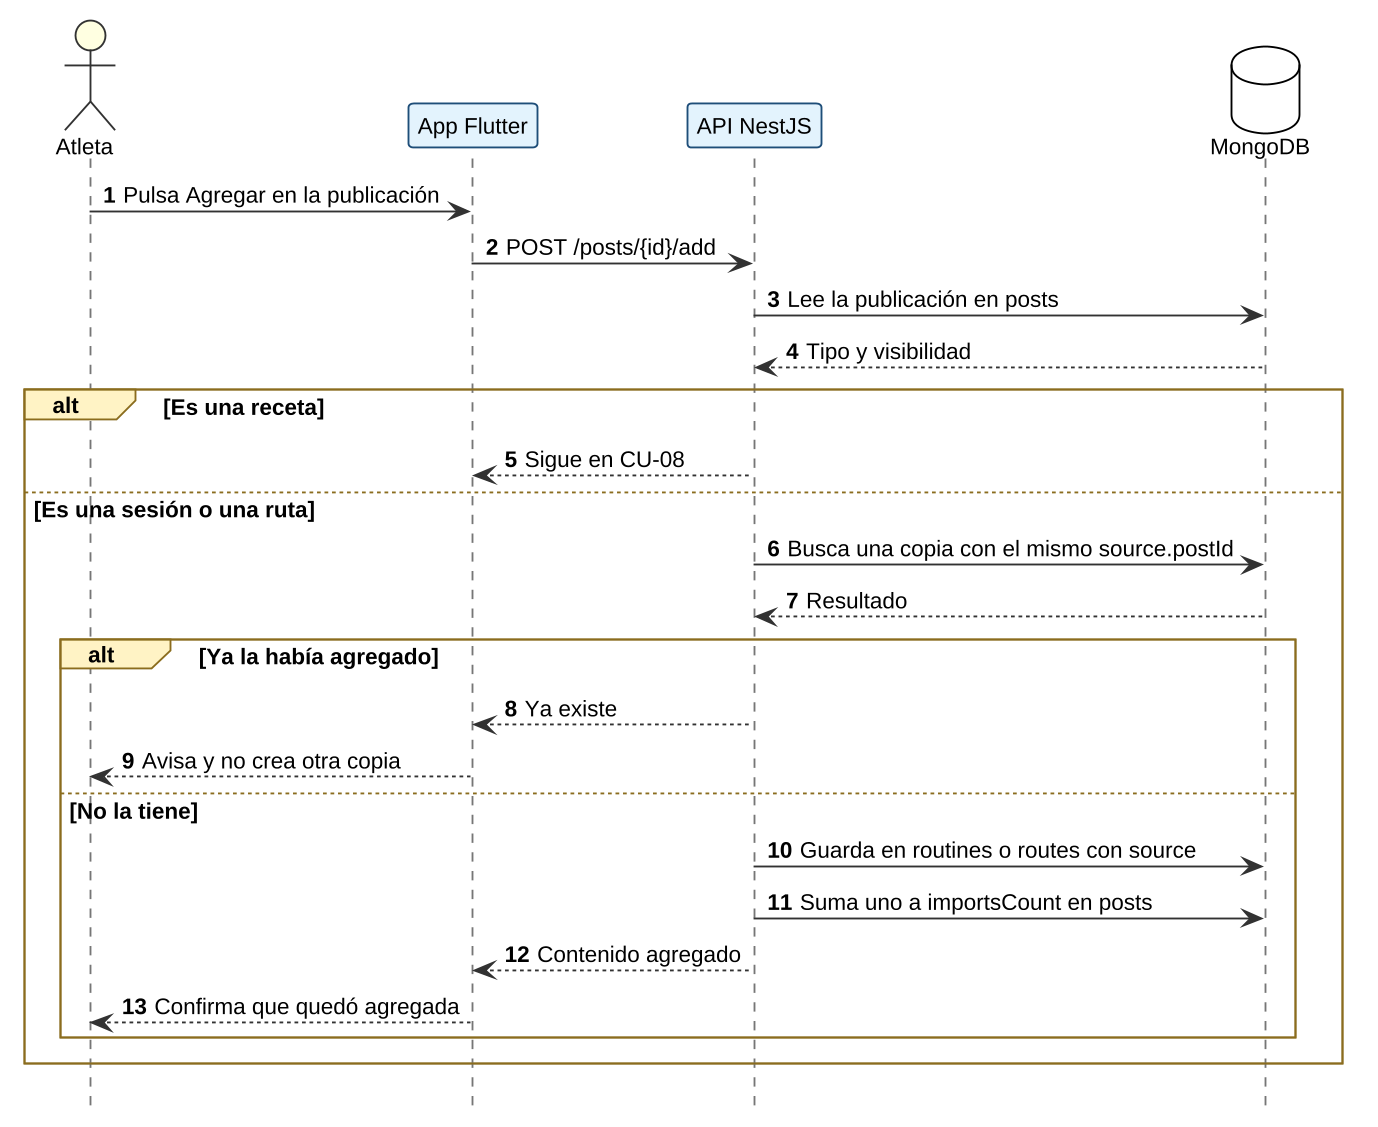
\includegraphics[width=0.95\textwidth,height=0.6\textheight,keepaspectratio]{figuras/secuencia/sec_cu13.png}
    \captionof{figure}{Diagrama de Secuencia -- CU-13: Agregar una publicación a mis módulos.}
    \label{fig:sec_cu13}
\end{center}
El backend identifica el tipo de publicación. Una sesión se copia en \texttt{routines} y una ruta en \texttt{routes}, con la referencia a su autor en el campo \texttt{source}, y se suma uno a \texttt{importsCount}. Antes revisa que el usuario no tenga ya esa copia. Las recetas siguen el flujo del CU-08.
\end{minipage}
\vspace{0.6cm}

\noindent\begin{minipage}{\linewidth}
\textbf{CU-14. Seguir a otro usuario}

Para el caso de uso CU-14 se genera el diagrama de secuencia que se muestra en la Figura \ref{fig:sec_cu14}.
\begin{center}
    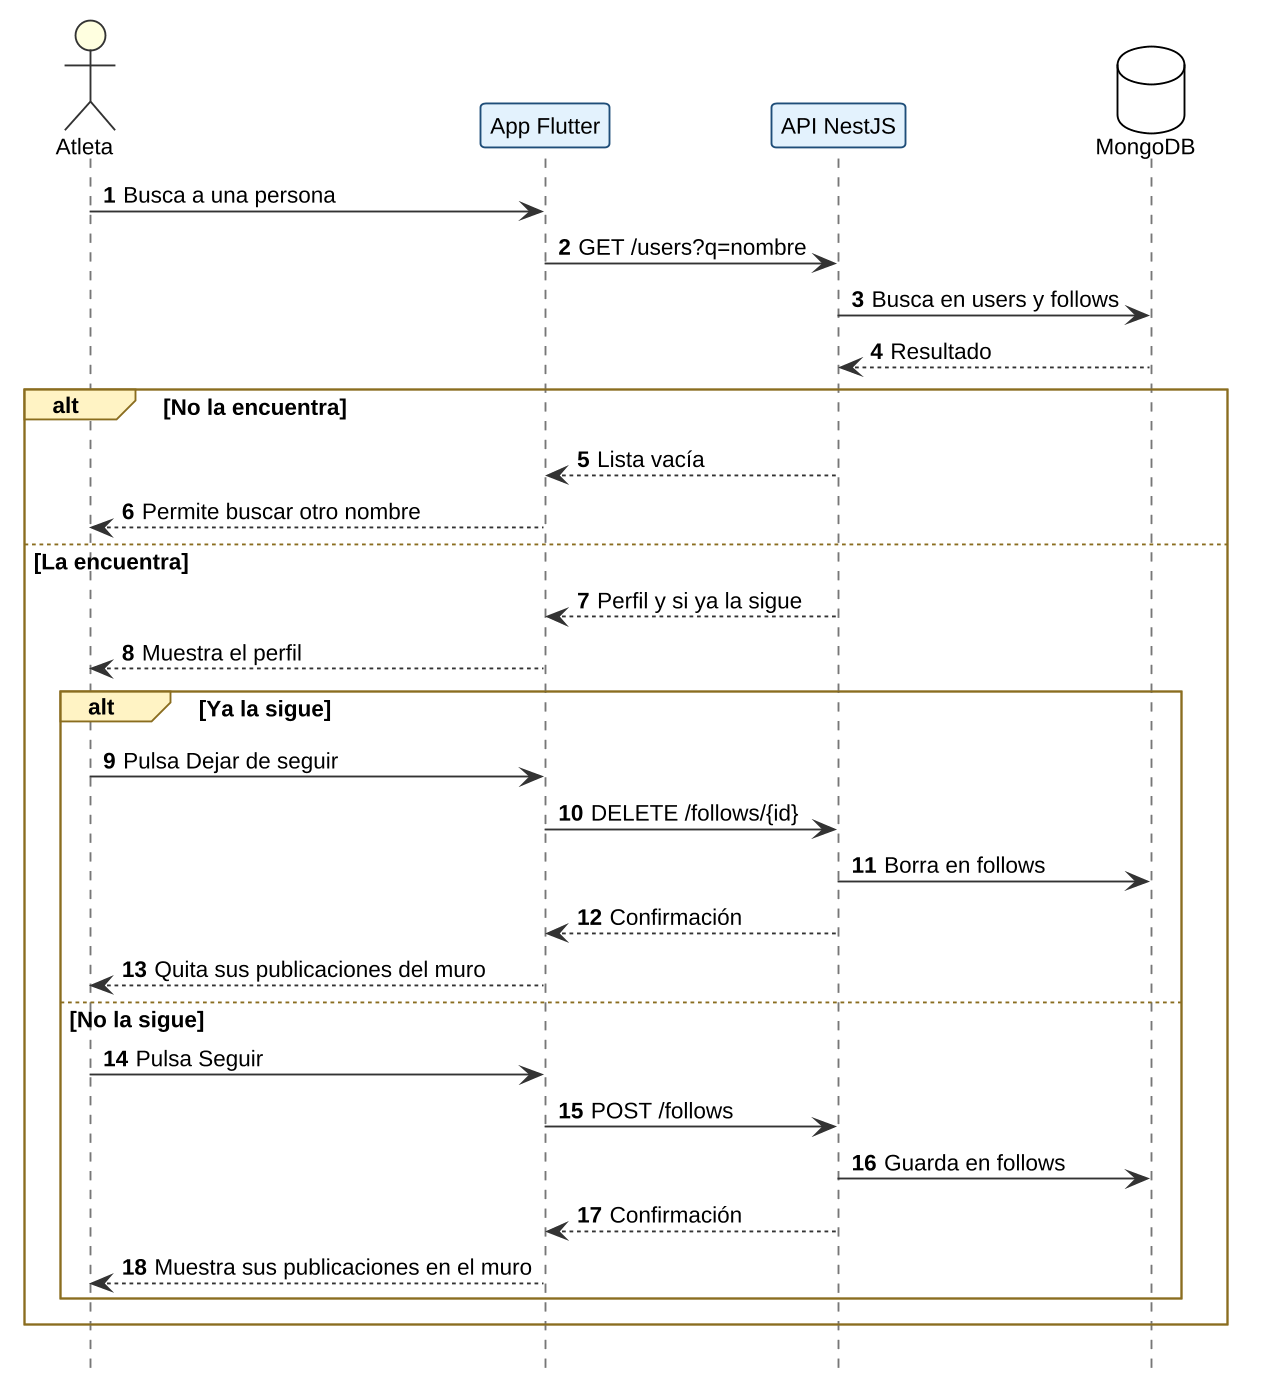
\includegraphics[width=0.95\textwidth,height=0.6\textheight,keepaspectratio]{figuras/secuencia/sec_cu14.png}
    \captionof{figure}{Diagrama de Secuencia -- CU-14: Seguir a otro usuario.}
    \label{fig:sec_cu14}
\end{center}
El backend busca a la persona y responde si el usuario ya la sigue. Seguir a alguien crea un documento en \texttt{follows}, y dejar de seguirlo lo borra. El muro se arma con estas relaciones (CU-23).
\end{minipage}
\vspace{0.6cm}

\noindent\begin{minipage}{\linewidth}
\textbf{CU-15. Registrar un producto con su código de barras}

Para el caso de uso CU-15 se genera el diagrama de secuencia que se muestra en la Figura \ref{fig:sec_cu15}.
\begin{center}
    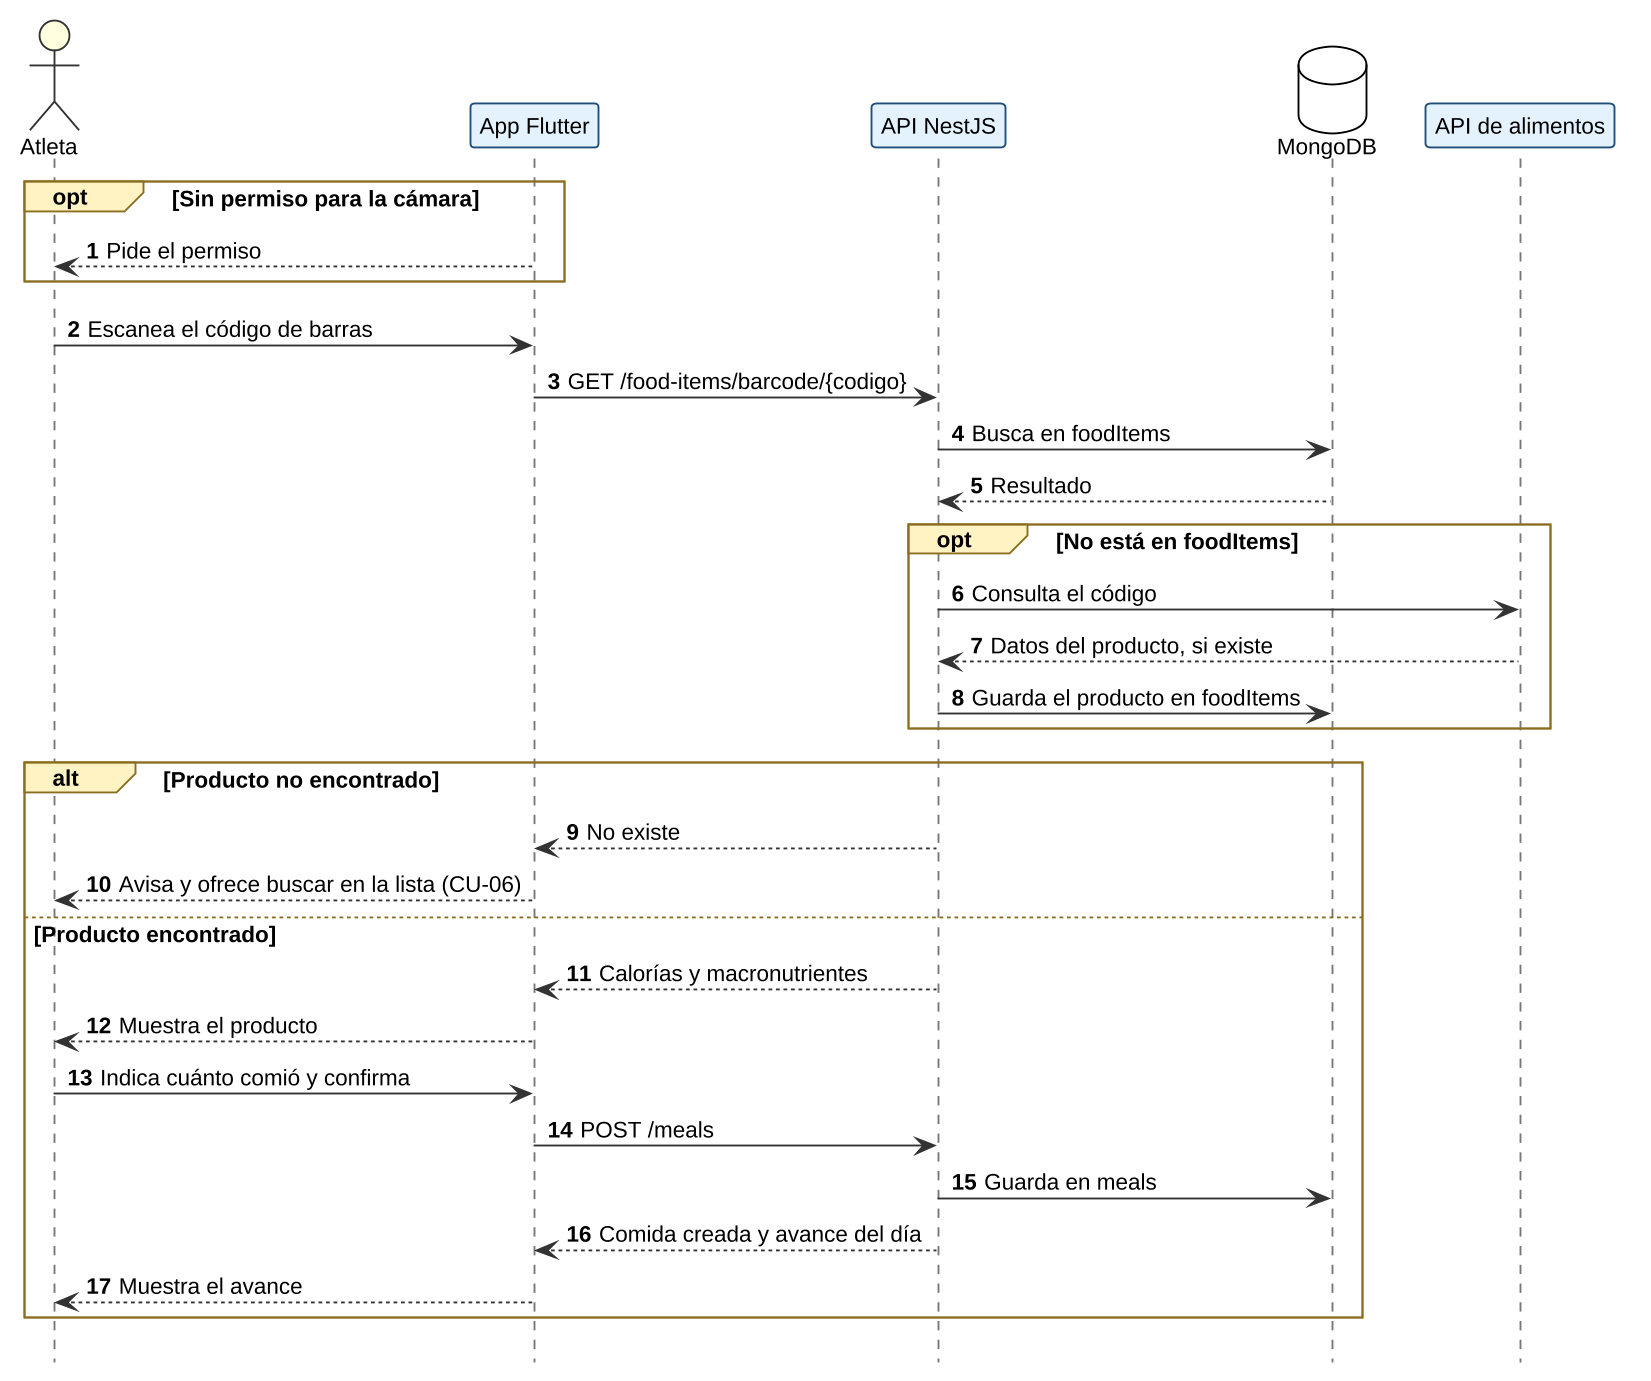
\includegraphics[width=0.95\textwidth,height=0.6\textheight,keepaspectratio]{figuras/secuencia/sec_cu15.png}
    \captionof{figure}{Diagrama de Secuencia -- CU-15: Registrar un producto con su código de barras.}
    \label{fig:sec_cu15}
\end{center}
El backend busca primero el código en \texttt{foodItems}. Si no está, consulta la API de alimentos y guarda el producto, para que las siguientes consultas sean más rápidas. Si el producto no existe en ninguna de las dos fuentes, se ofrece buscarlo en la lista.
\end{minipage}
\vspace{0.6cm}

\noindent\begin{minipage}{\linewidth}
\textbf{CU-16. Contar mi comida con mis palabras}

Para el caso de uso CU-16 se genera el diagrama de secuencia que se muestra en la Figura \ref{fig:sec_cu16}.
\begin{center}
    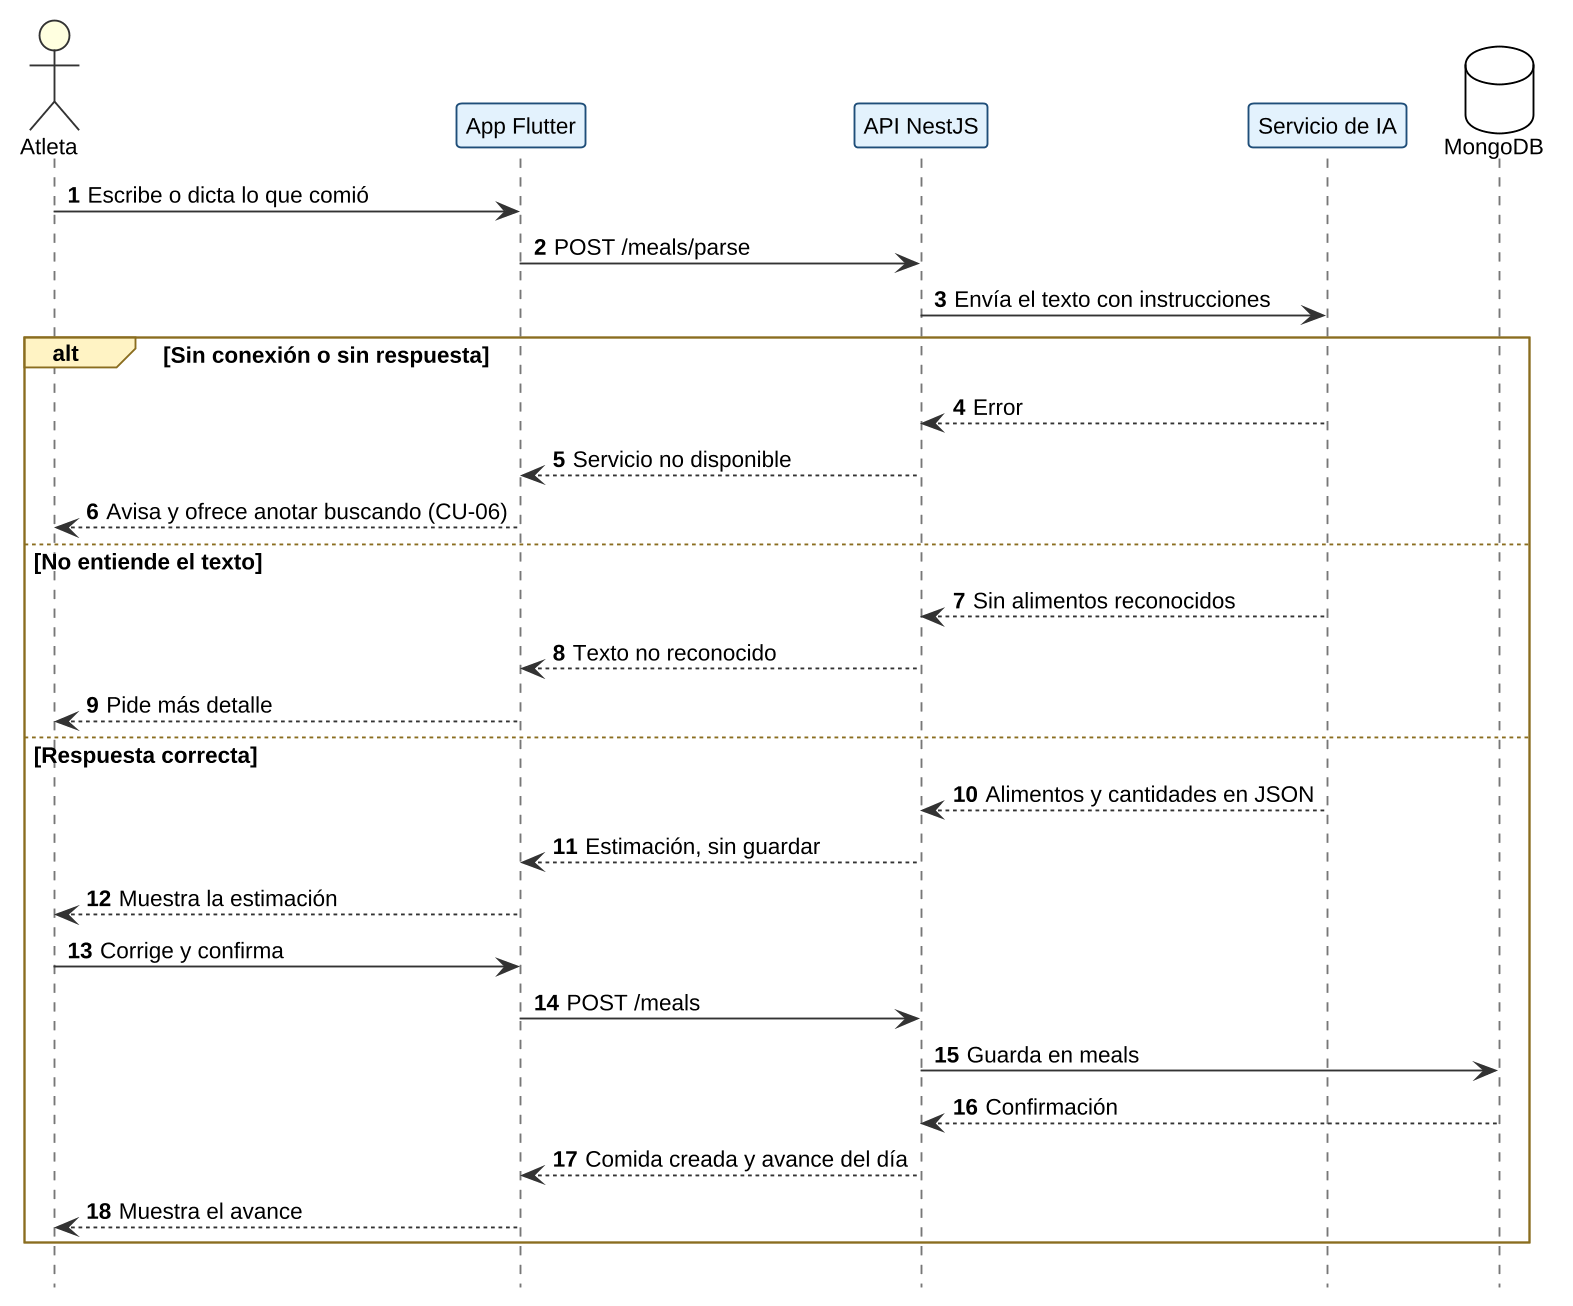
\includegraphics[width=0.95\textwidth,height=0.6\textheight,keepaspectratio]{figuras/secuencia/sec_cu16.png}
    \captionof{figure}{Diagrama de Secuencia -- CU-16: Contar mi comida con mis palabras.}
    \label{fig:sec_cu16}
\end{center}
El flujo es parecido al del CU-07, pero con texto en vez de una foto. El backend envía la descripción al servicio de IA y devuelve una estimación sin guardarla. Si el texto no se entiende, se pide más detalle. La comida se guarda solo cuando el usuario confirma.
\end{minipage}
\vspace{0.6cm}

\noindent\begin{minipage}{\linewidth}
\textbf{CU-17. Registrar una sesión de cardio sin reloj}

Para el caso de uso CU-17 se genera el diagrama de secuencia que se muestra en la Figura \ref{fig:sec_cu17}.
\begin{center}
    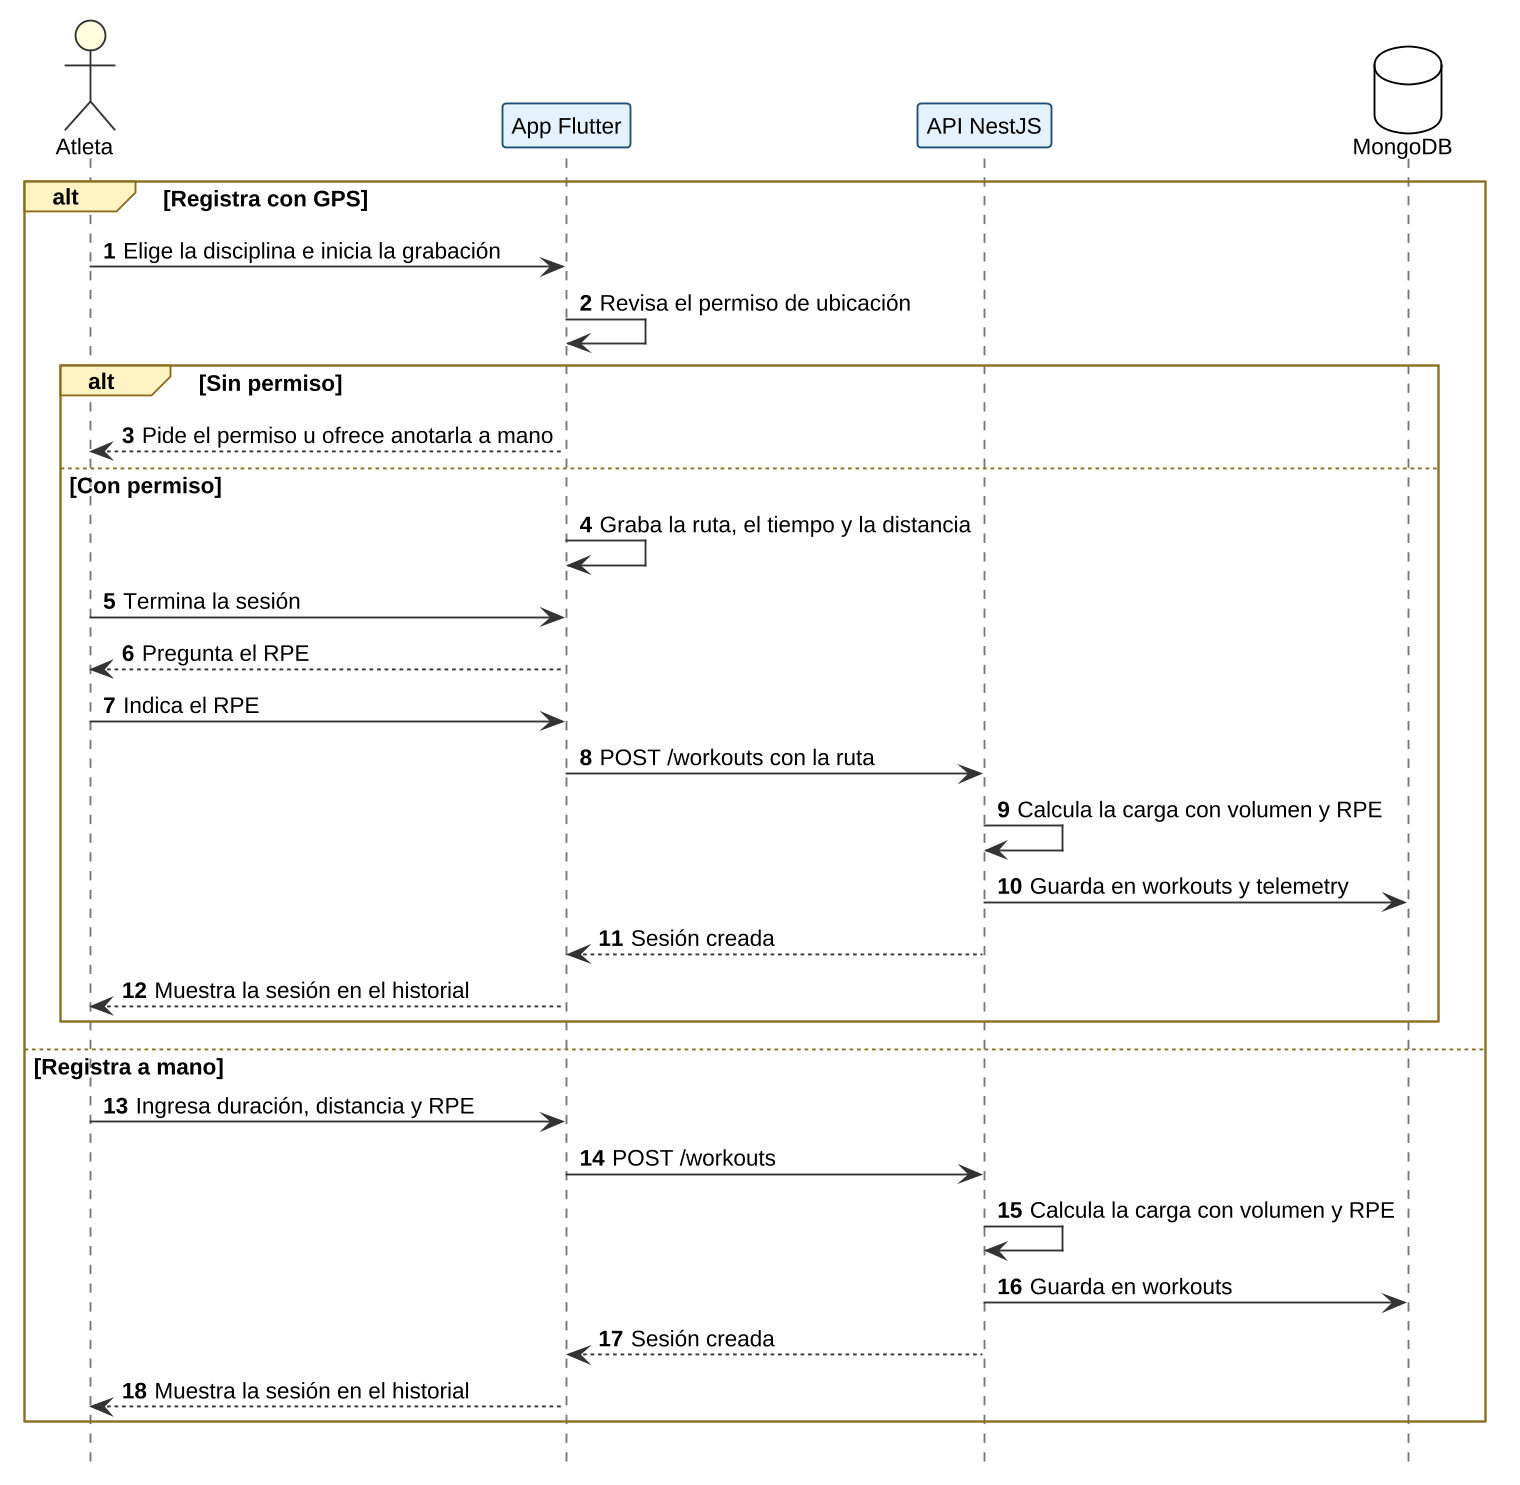
\includegraphics[width=0.95\textwidth,height=0.6\textheight,keepaspectratio]{figuras/secuencia/sec_cu17.png}
    \captionof{figure}{Diagrama de Secuencia -- CU-17: Registrar una sesión de cardio sin reloj.}
    \label{fig:sec_cu17}
\end{center}
La grabación con GPS ocurre en el teléfono, por lo que no necesita conexión mientras dura la sesión. Al terminar, la aplicación envía la ruta y el RPE. Sin dispositivos externos, la carga se calcula con el volumen de la sesión y el RPE. El registro a mano sigue el mismo camino, pero sin ruta.
\end{minipage}
\vspace{0.6cm}

\noindent\begin{minipage}{\linewidth}
\textbf{CU-18. Ver mis metas de alimentación del día}

Para el caso de uso CU-18 se genera el diagrama de secuencia que se muestra en la Figura \ref{fig:sec_cu18}.
\begin{center}
    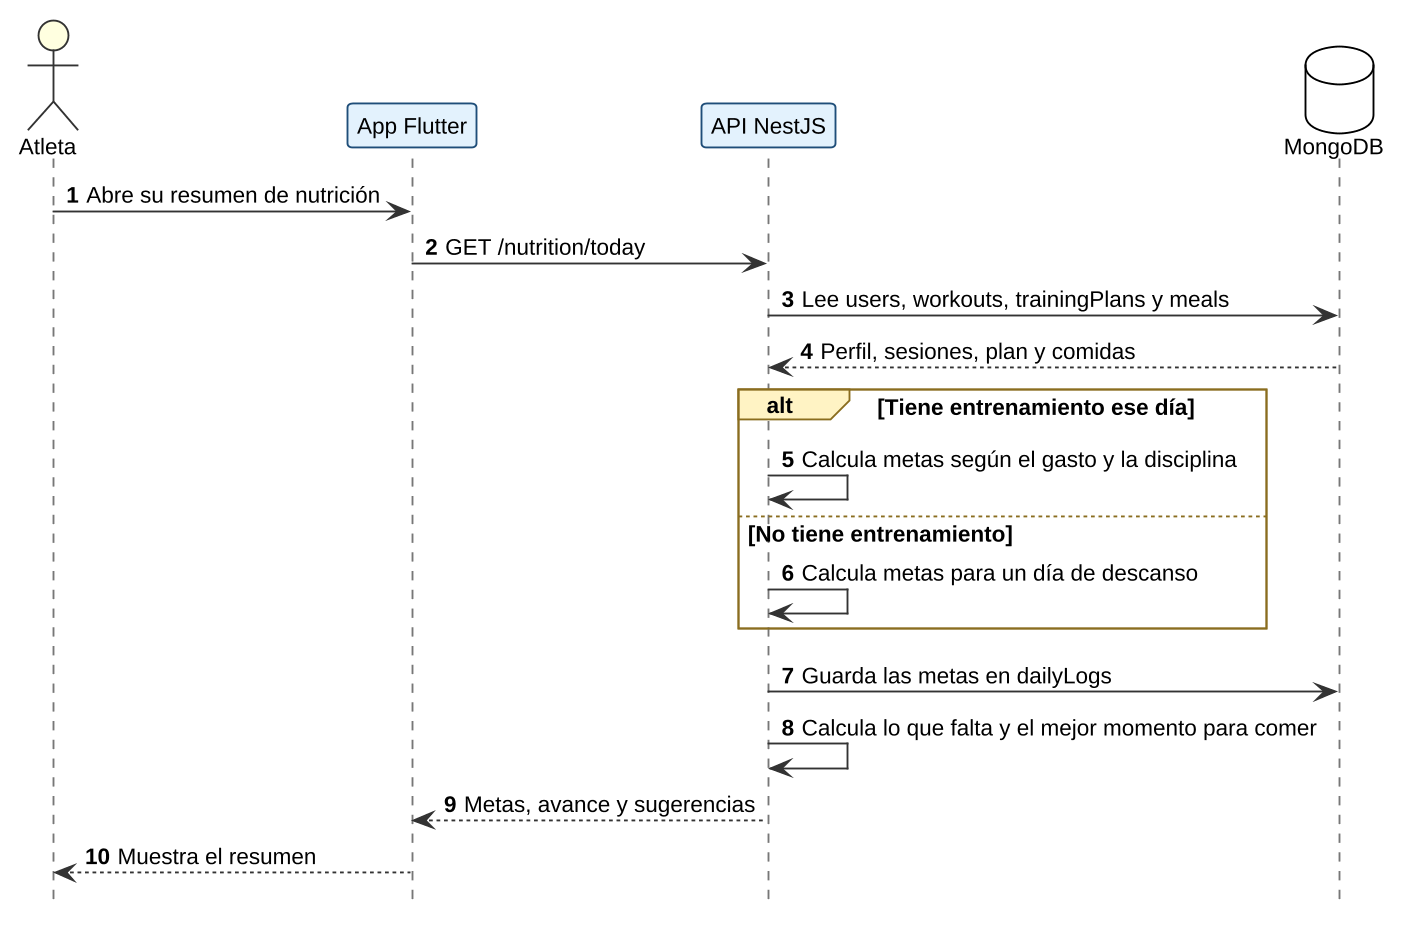
\includegraphics[width=0.95\textwidth,height=0.6\textheight,keepaspectratio]{figuras/secuencia/sec_cu18.png}
    \captionof{figure}{Diagrama de Secuencia -- CU-18: Ver mis metas de alimentación del día.}
    \label{fig:sec_cu18}
\end{center}
El backend lee el perfil, las sesiones, el plan y las comidas del día. Con eso calcula las metas según el gasto estimado y la disciplina, o las metas de un día de descanso si no hay entrenamiento. Las guarda en \texttt{dailyLogs} y responde con el avance y las sugerencias de horario.
\end{minipage}
\vspace{0.6cm}

\noindent\begin{minipage}{\linewidth}
\textbf{CU-19. Revisar mi progreso}

Para el caso de uso CU-19 se genera el diagrama de secuencia que se muestra en la Figura \ref{fig:sec_cu19}.
\begin{center}
    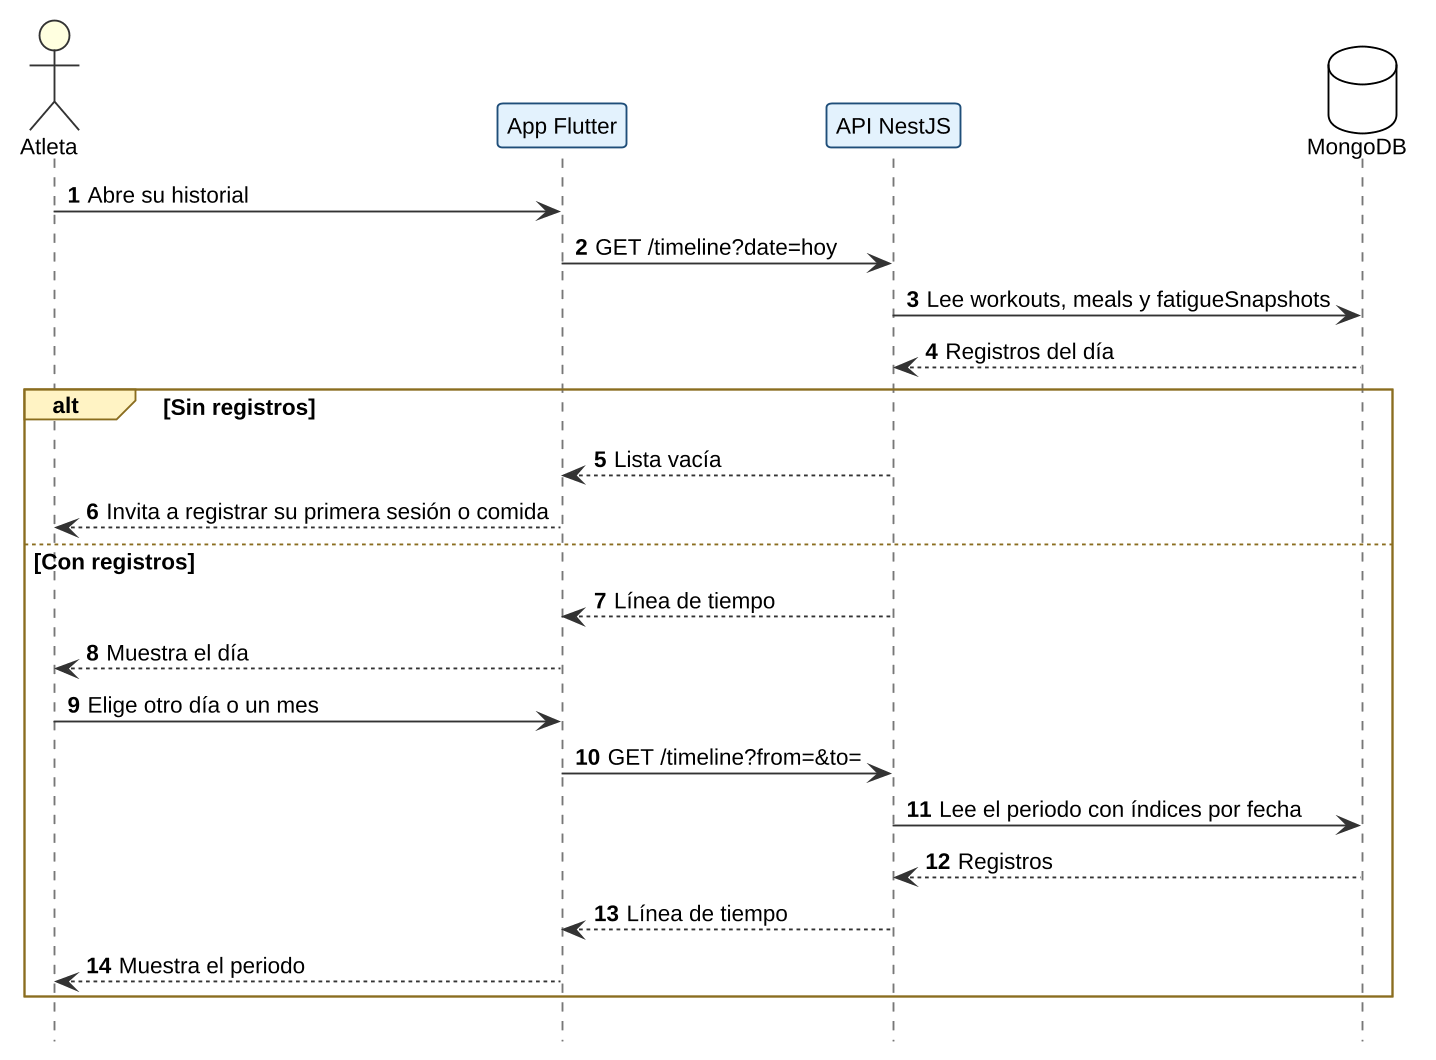
\includegraphics[width=0.95\textwidth,height=0.6\textheight,keepaspectratio]{figuras/secuencia/sec_cu19.png}
    \captionof{figure}{Diagrama de Secuencia -- CU-19: Revisar mi progreso.}
    \label{fig:sec_cu19}
\end{center}
El historial se arma consultando por usuario y fecha en \texttt{workouts}, \texttt{meals} y \texttt{fatigueSnapshots}. Los índices compuestos por usuario y fecha hacen que esta consulta sea rápida, tanto para un día como para un mes.
\end{minipage}
\vspace{0.6cm}

\noindent\begin{minipage}{\linewidth}
\textbf{CU-20. Anotar cómo me sentí}

Para el caso de uso CU-20 se genera el diagrama de secuencia que se muestra en la Figura \ref{fig:sec_cu20}.
\begin{center}
    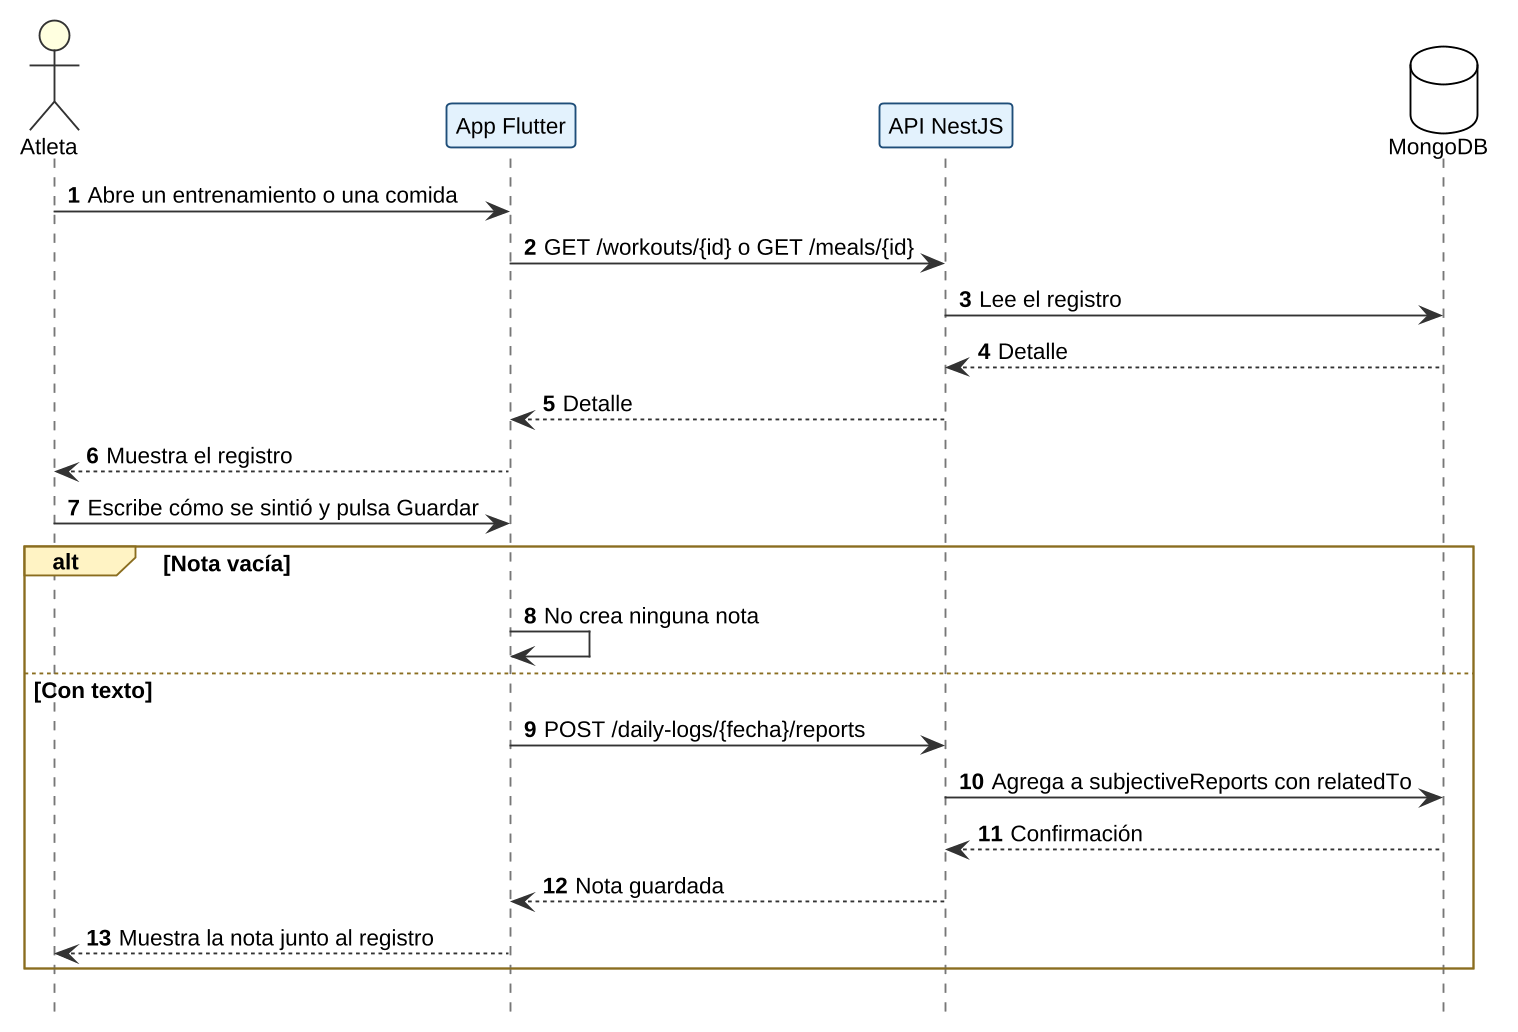
\includegraphics[width=0.95\textwidth,height=0.6\textheight,keepaspectratio]{figuras/secuencia/sec_cu20.png}
    \captionof{figure}{Diagrama de Secuencia -- CU-20: Anotar cómo me sentí.}
    \label{fig:sec_cu20}
\end{center}
La nota se guarda en \texttt{subjectiveReports}, dentro del registro diario, con el campo \texttt{relatedTo}, que indica a qué entrenamiento o comida pertenece. Si el usuario no escribe nada, la aplicación no hace ninguna llamada al backend.
\end{minipage}
\vspace{0.6cm}

\noindent\begin{minipage}{\linewidth}
\textbf{CU-21. Controlar mis datos personales}

Para el caso de uso CU-21 se genera el diagrama de secuencia que se muestra en la Figura \ref{fig:sec_cu21}.
\begin{center}
    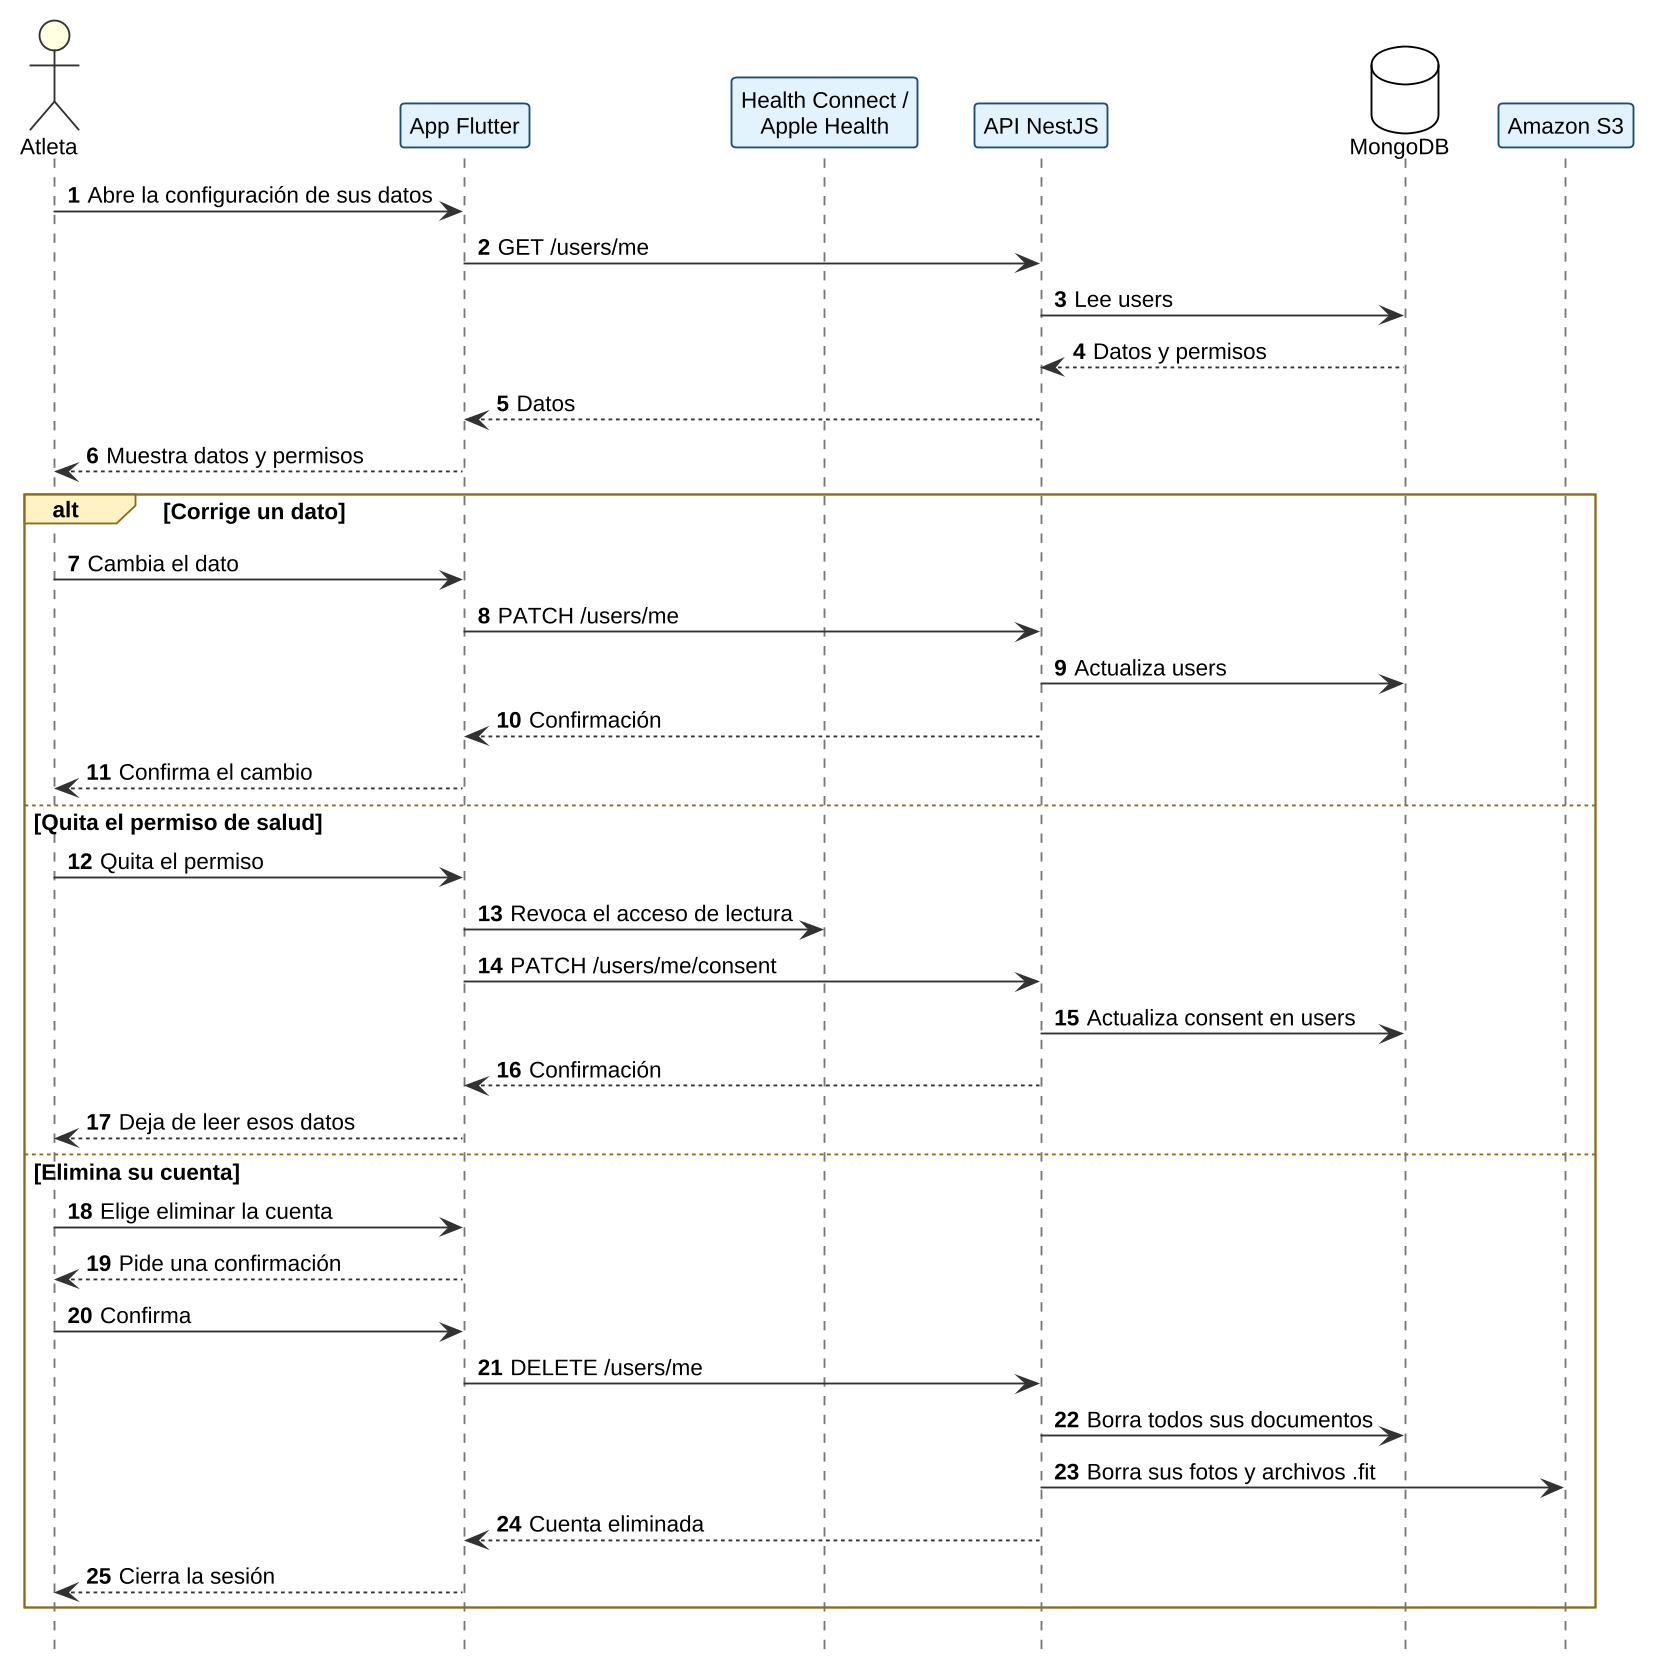
\includegraphics[width=0.95\textwidth,height=0.6\textheight,keepaspectratio]{figuras/secuencia/sec_cu21.png}
    \captionof{figure}{Diagrama de Secuencia -- CU-21: Controlar mis datos personales.}
    \label{fig:sec_cu21}
\end{center}
Los cambios de datos se guardan en \texttt{users}. Quitar el permiso de salud corta el acceso en el teléfono y queda registrado en \texttt{consent}. Al eliminar la cuenta, el backend borra todos los documentos del usuario en MongoDB y sus archivos en Amazon S3, como exige la Ley N° 19.628.
\end{minipage}
\vspace{0.6cm}

\noindent\begin{minipage}{\linewidth}
\textbf{CU-22. Reportar una publicación}

Para el caso de uso CU-22 se genera el diagrama de secuencia que se muestra en la Figura \ref{fig:sec_cu22}.
\begin{center}
    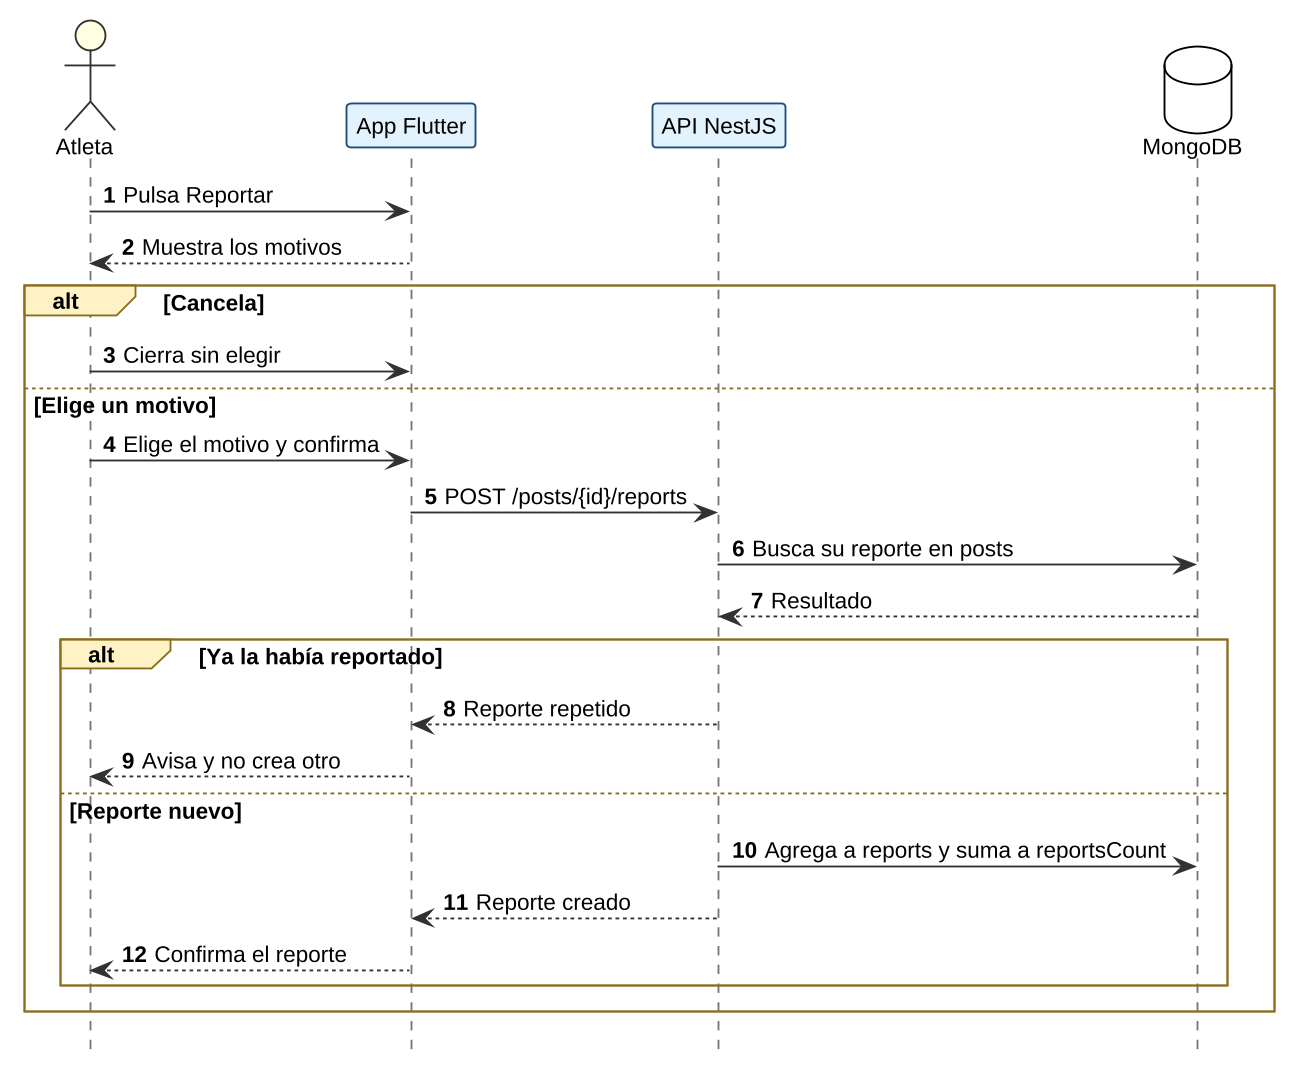
\includegraphics[width=0.95\textwidth,height=0.6\textheight,keepaspectratio]{figuras/secuencia/sec_cu22.png}
    \captionof{figure}{Diagrama de Secuencia -- CU-22: Reportar una publicación.}
    \label{fig:sec_cu22}
\end{center}
El backend revisa en el arreglo \texttt{reports} de la publicación que el usuario no la haya reportado antes. Si no lo ha hecho, agrega el reporte con su motivo y suma uno a \texttt{reportsCount}. Con esto la publicación aparece en la lista de revisión del administrador (CU-11).
\end{minipage}
\vspace{0.6cm}

\noindent\begin{minipage}{\linewidth}
\textbf{CU-23. Ver el muro de la comunidad}

Para el caso de uso CU-23 se genera el diagrama de secuencia que se muestra en la Figura \ref{fig:sec_cu23}.
\begin{center}
    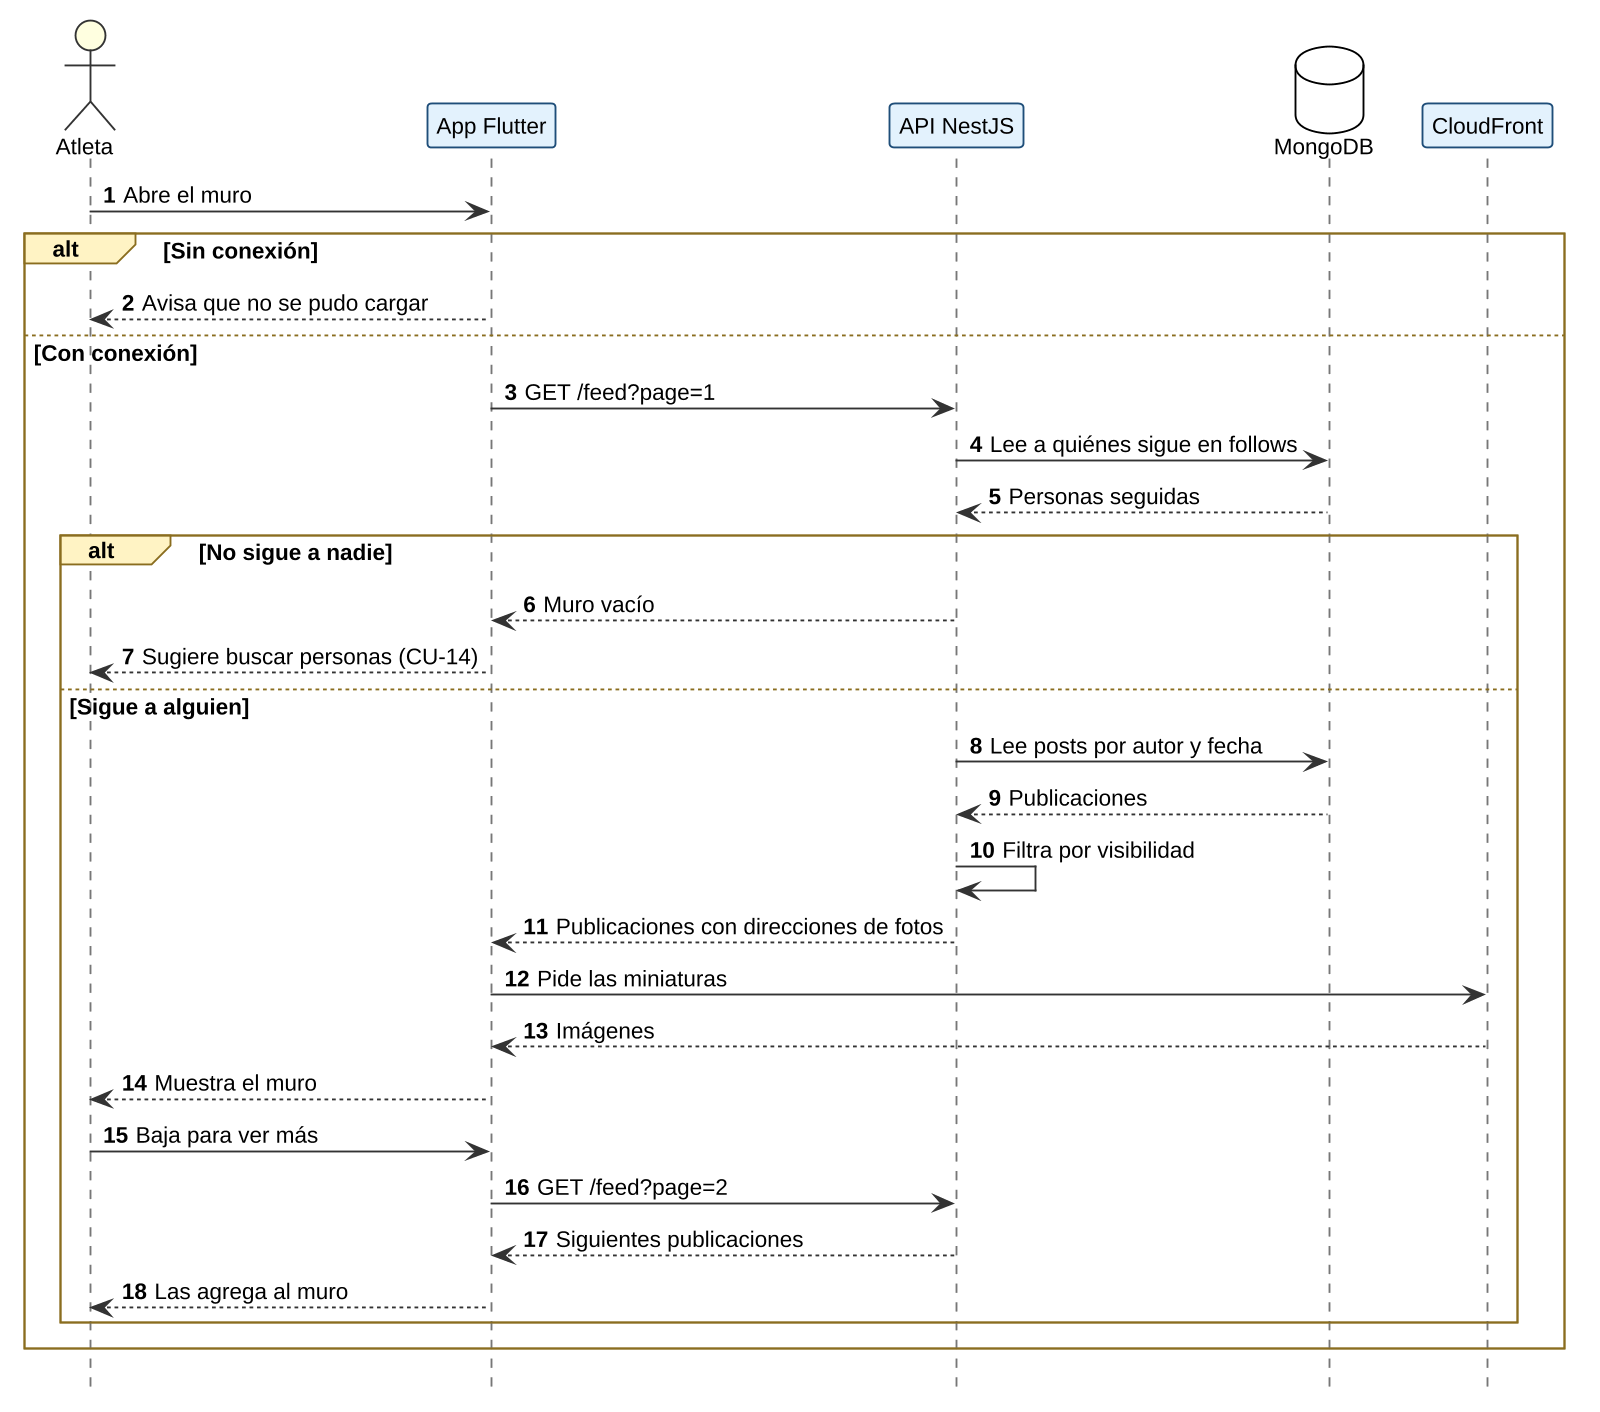
\includegraphics[width=0.95\textwidth,height=0.6\textheight,keepaspectratio]{figuras/secuencia/sec_cu23.png}
    \captionof{figure}{Diagrama de Secuencia -- CU-23: Ver el muro de la comunidad.}
    \label{fig:sec_cu23}
\end{center}
El backend lee a quiénes sigue el usuario en \texttt{follows}, busca sus publicaciones más recientes en \texttt{posts} y filtra las que puede ver según su visibilidad. La respuesta llega por páginas y solo trae las direcciones de las fotos. La aplicación las pide después a CloudFront, sin pasar por el backend.
\end{minipage}
\vspace{0.6cm}

\noindent\begin{minipage}{\linewidth}
\textbf{CU-24. Contratar el plan premium}

Para el caso de uso CU-24 se genera el diagrama de secuencia que se muestra en la Figura \ref{fig:sec_cu24}.
\begin{center}
    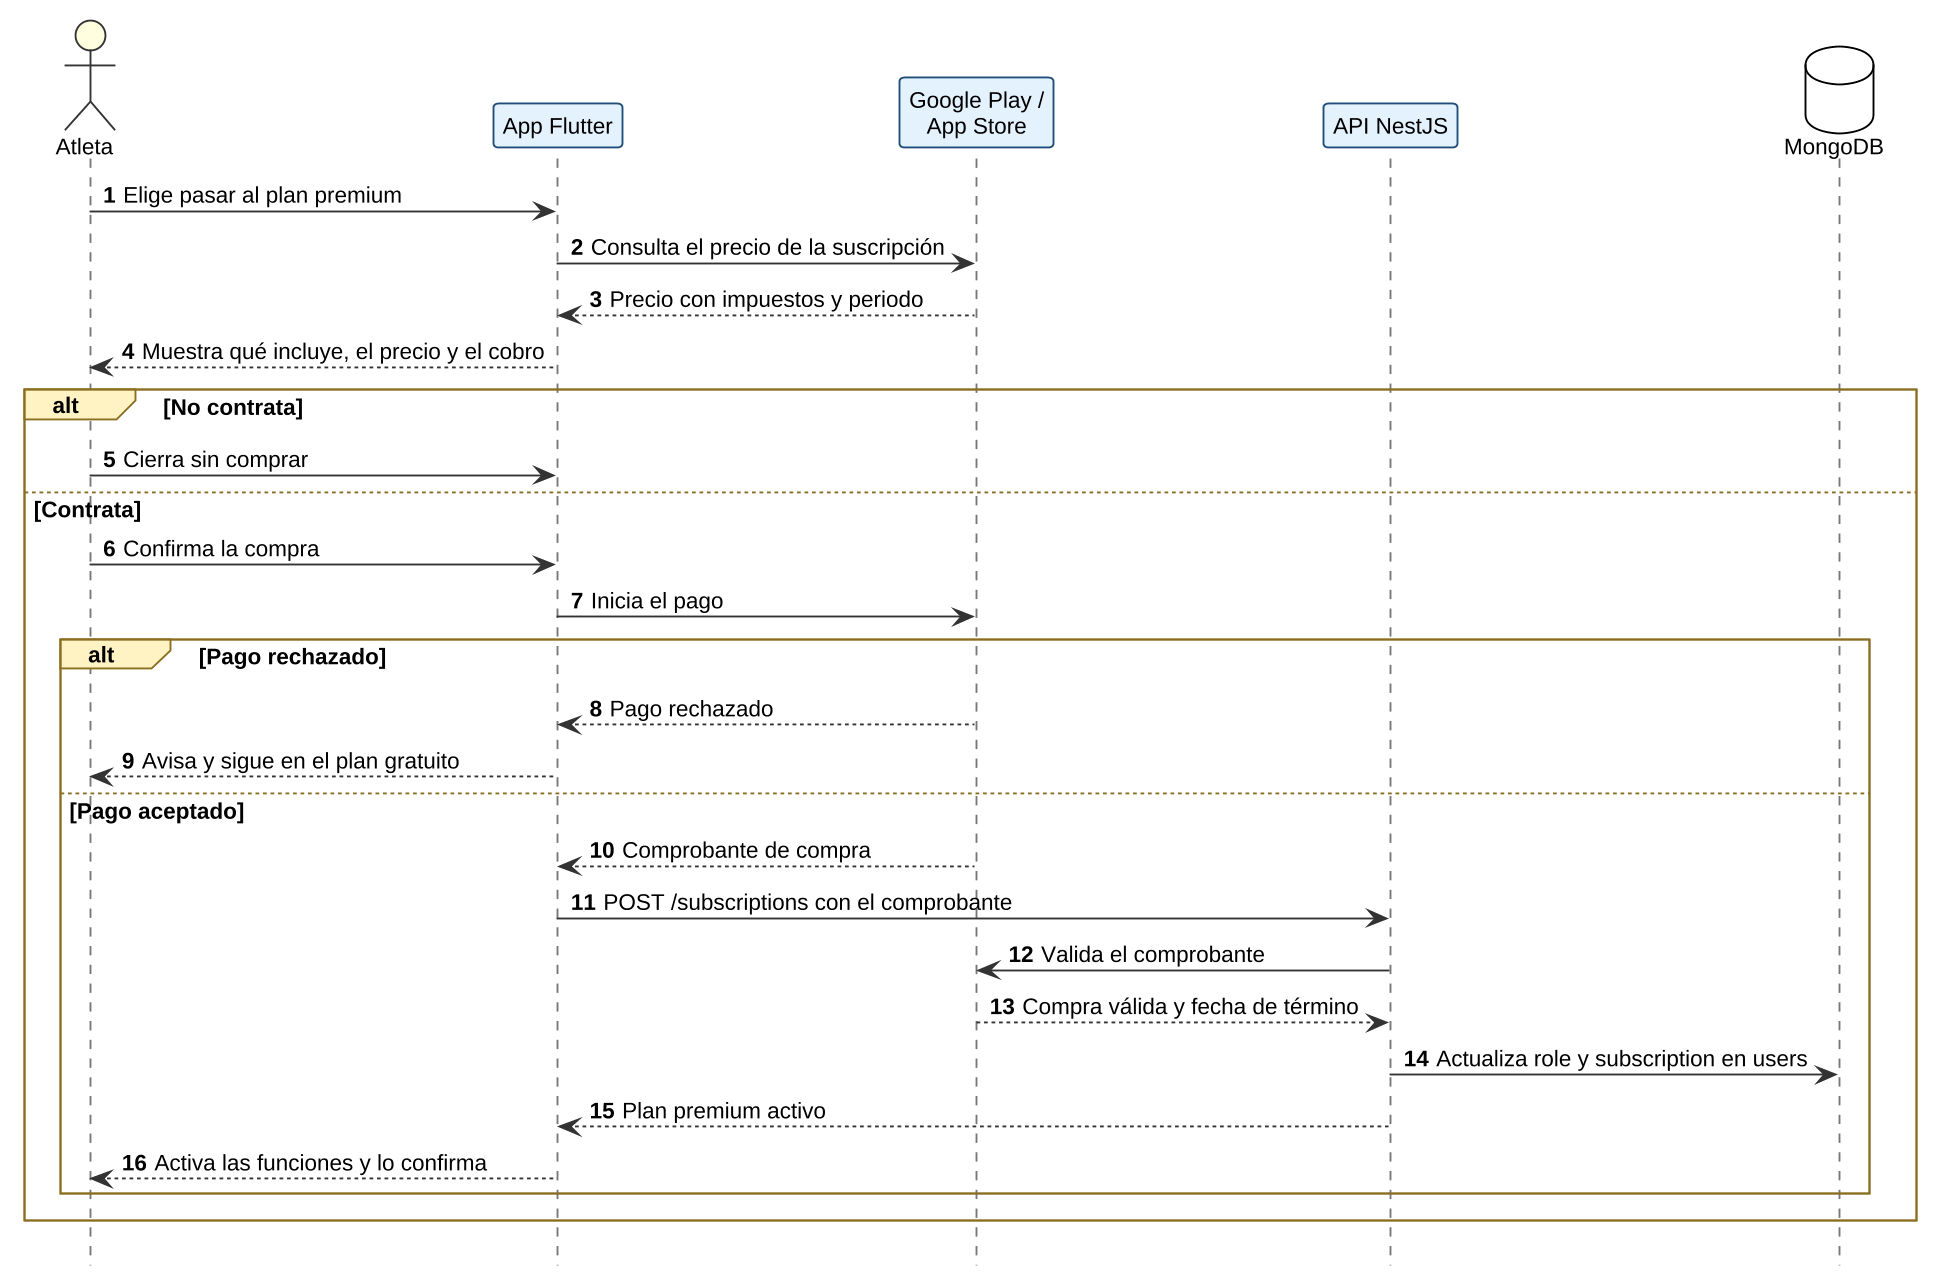
\includegraphics[width=0.95\textwidth,height=0.6\textheight,keepaspectratio]{figuras/secuencia/sec_cu24.png}
    \captionof{figure}{Diagrama de Secuencia -- CU-24: Contratar el plan premium.}
    \label{fig:sec_cu24}
\end{center}
El precio viene de la tienda, para mostrar el valor final con impuestos. El pago ocurre completo en Google Play o App Store, por lo que el sistema no maneja datos de tarjetas. Al terminar, la aplicación envía el comprobante al backend, que lo valida con la tienda antes de activar el plan en \texttt{users}.
\end{minipage}
\vspace{0.6cm}

\noindent\begin{minipage}{\linewidth}
\textbf{CU-25. Cancelar mi suscripción}

Para el caso de uso CU-25 se genera el diagrama de secuencia que se muestra en la Figura \ref{fig:sec_cu25}.
\begin{center}
    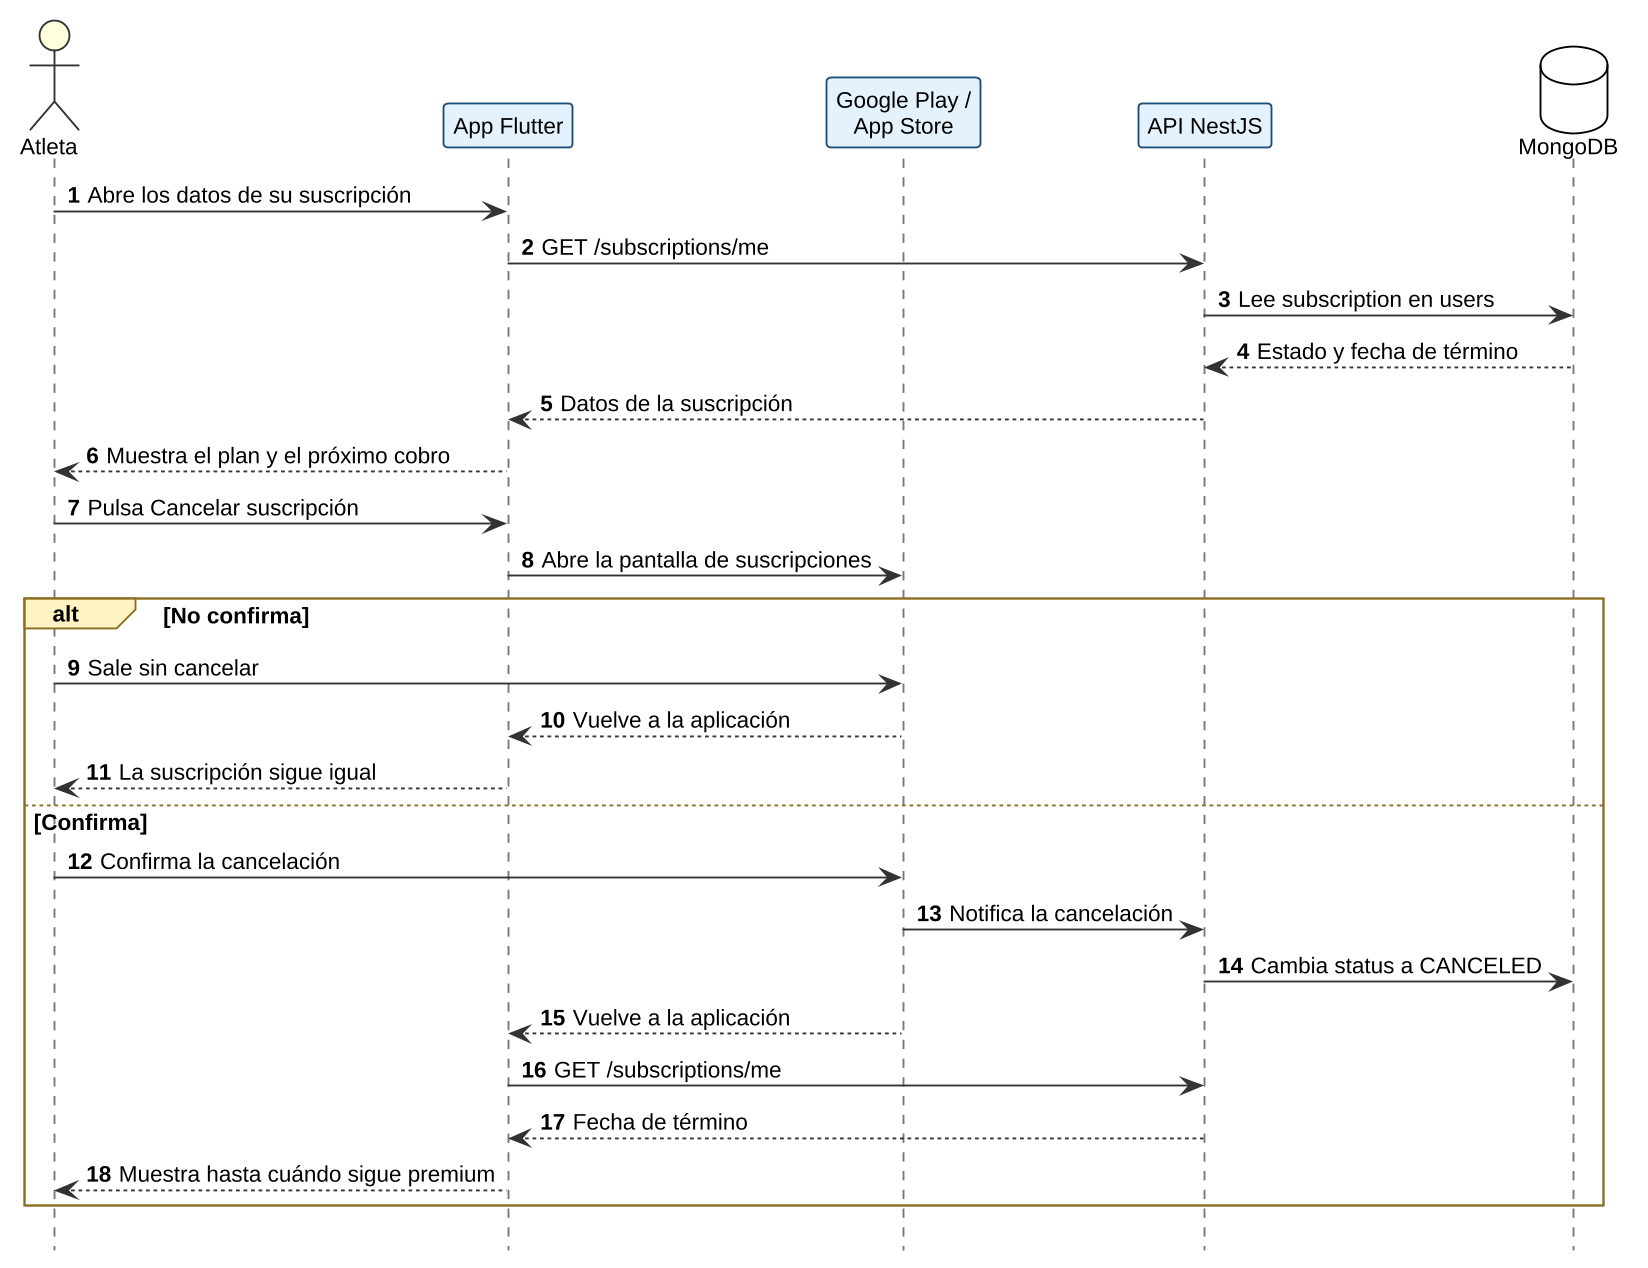
\includegraphics[width=0.95\textwidth,height=0.6\textheight,keepaspectratio]{figuras/secuencia/sec_cu25.png}
    \captionof{figure}{Diagrama de Secuencia -- CU-25: Cancelar mi suscripción.}
    \label{fig:sec_cu25}
\end{center}
La cancelación se confirma en la pantalla de suscripciones de la tienda. La tienda avisa al backend, que cambia el estado de la suscripción a \texttt{CANCELED}. El usuario mantiene el plan premium hasta la fecha guardada en \texttt{expiresAt}, y luego vuelve al plan gratuito con todos sus datos.
\end{minipage}
\vspace{0.6cm}

\noindent\begin{minipage}{\linewidth}
\textbf{CU-26. Aceptar los términos de uso y el aviso legal}

Para el caso de uso CU-26 se genera el diagrama de secuencia que se muestra en la Figura \ref{fig:sec_cu26}.
\begin{center}
    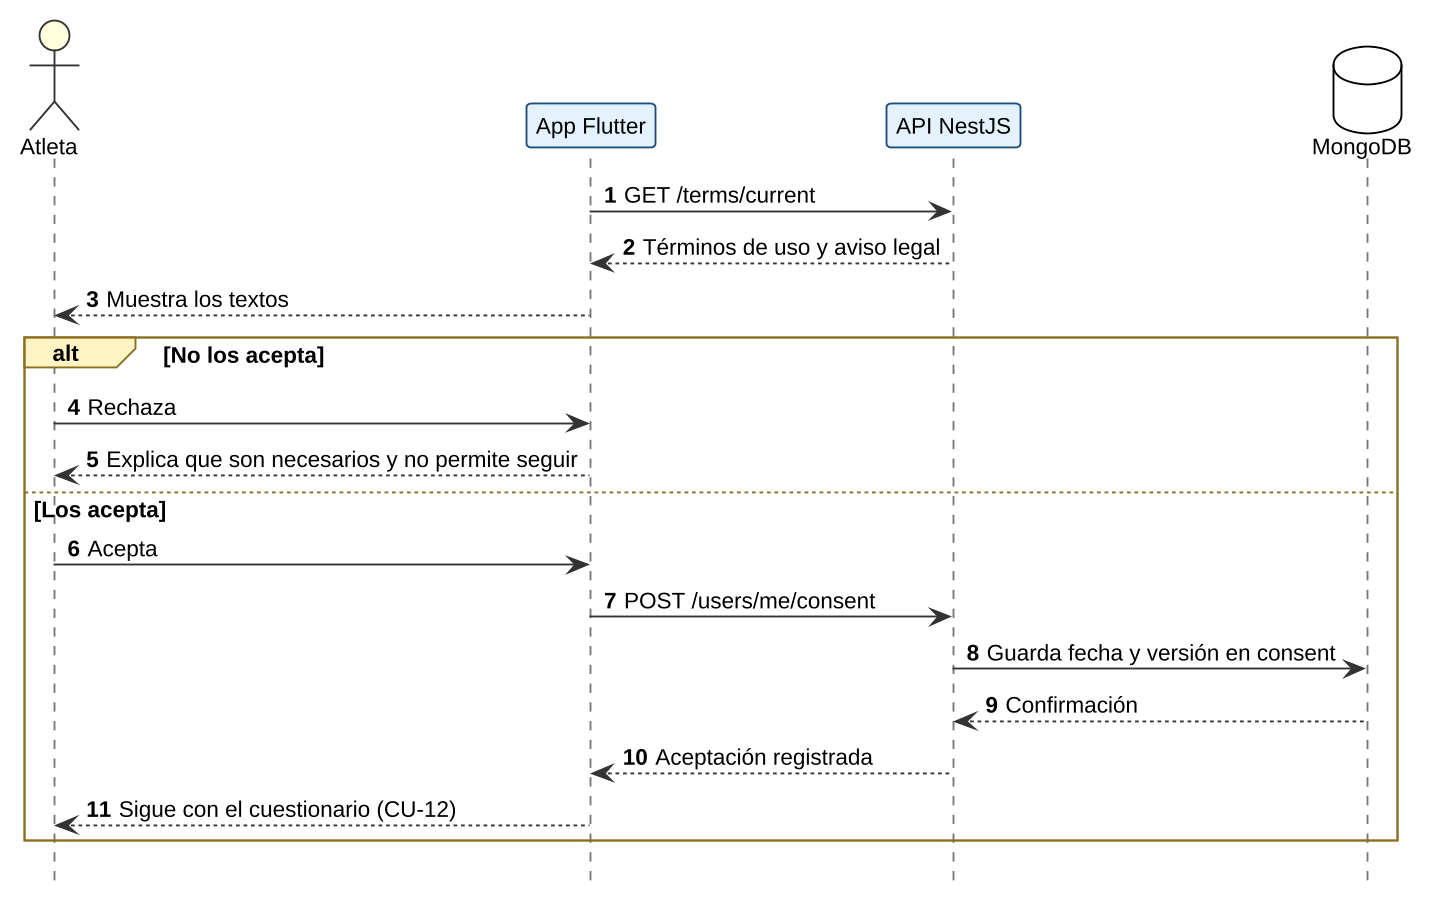
\includegraphics[width=0.95\textwidth,height=0.6\textheight,keepaspectratio]{figuras/secuencia/sec_cu26.png}
    \captionof{figure}{Diagrama de Secuencia -- CU-26: Aceptar los términos de uso y el aviso legal.}
    \label{fig:sec_cu26}
\end{center}
La aplicación pide al backend la versión vigente de los textos. Si el usuario los acepta, el backend guarda la fecha y la versión en \texttt{consent}, para poder demostrar qué aceptó. Sin esta aceptación no se puede seguir con el cuestionario inicial.
\end{minipage}
\vspace{0.6cm}

\noindent\begin{minipage}{\linewidth}
\textbf{CU-27. Crear una receta}

Para el caso de uso CU-27 se genera el diagrama de secuencia que se muestra en la Figura \ref{fig:sec_cu27}.
\begin{center}
    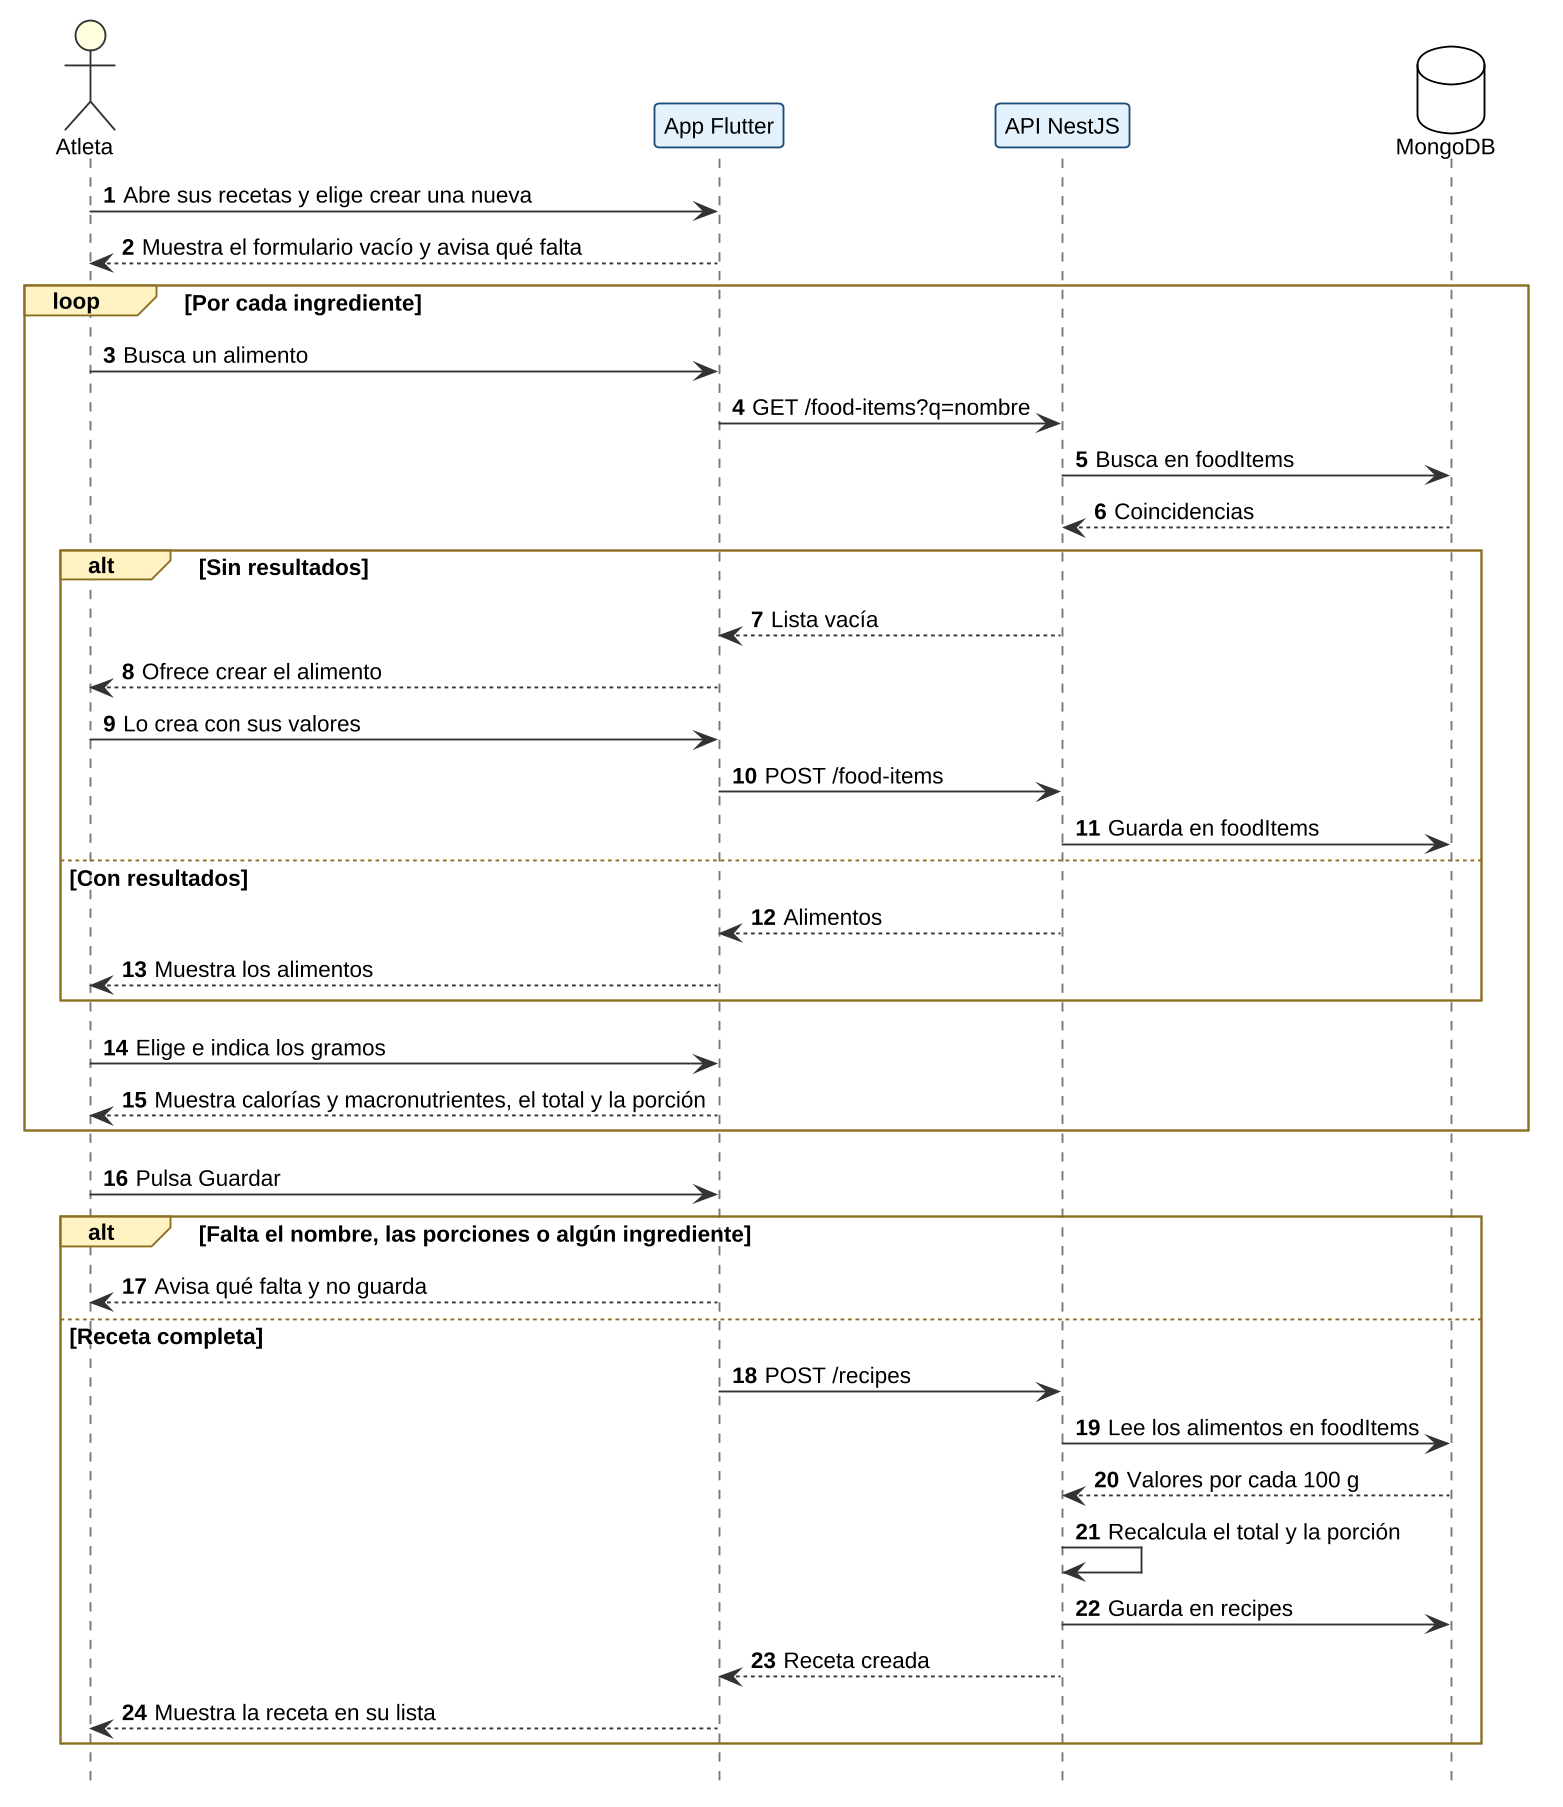
\includegraphics[width=0.95\textwidth,height=0.6\textheight,keepaspectratio]{figuras/secuencia/sec_cu27.png}
    \captionof{figure}{Diagrama de Secuencia -- CU-27: Crear una receta.}
    \label{fig:sec_cu27}
\end{center}
Por cada ingrediente, la aplicación busca en el catálogo \texttt{foodItems} a través del backend, y si el alimento no existe permite crearlo. Mientras el usuario arma la receta, la aplicación muestra los valores calculados, pero al guardar el backend los recalcula con los datos del catálogo y no confía en los que envía el teléfono. La receta se guarda en \texttt{recipes}, con su autor, y parte como privada. Si el usuario la publica después, se sigue el caso de uso CU-09.
\end{minipage}
\vspace{0.6cm}

\subsection{Diseño de Interfaces de Usuario}
En esta sección se muestran las pantallas que cubren cada caso de uso. Se construyeron en la aplicación Flutter del prototipo, y no en una herramienta de dibujo, para que el diseño sirva como base del desarrollo. El administrador usa un panel web, según lo definido en la arquitectura.

La interfaz usa Material Design 3 como base y agrega patrones de iOS, como las tarjetas agrupadas y las transiciones entre pantallas. Se organiza en cuatro módulos, que se eligen en el selector superior: nutrición, fuerza, cardio y comunidad. Cada módulo tiene sus secciones en la barra inferior. La paleta de colores es Gruvbox, con una versión clara y otra oscura, y cada macronutriente mantiene siempre su color. Las figuras de esta sección usan el modo claro, porque se lee mejor en una hoja impresa, aunque la aplicación también cuenta con el modo oscuro exigido en los requisitos de las interfaces.

\newlength{\uiancho}\setlength{\uiancho}{3.2cm}
\newlength{\uiescritorio}\setlength{\uiescritorio}{7.85cm}
\newcommand{\uifoto}[1]{\includegraphics[width=\uiancho]{figuras/interfaces/#1.jpg}}
\newcommand{\uiweb}[1]{\includegraphics[width=\uiescritorio]{figuras/interfaces/#1.jpg}}
\newcommand{\uitexto}[1]{{\setstretch{1.1}\small #1\par}}
% Cuatro pantallas: el texto va arriba.
\newcommand{\uicuatro}[8]{%
\noindent\begin{minipage}{\linewidth}
\textbf{#1}\par\vspace{0.1cm}
\uitexto{#2}\vspace{0.2cm}
\centering\uifoto{#3}\hspace{0.45cm}\uifoto{#4}\hspace{0.45cm}\uifoto{#5}\hspace{0.45cm}\uifoto{#6}
\captionof{figure}{Interfaces -- #7.}\label{#8}
\end{minipage}\par\vspace{0.3cm}}
% Tres pantallas: el texto va a la izquierda.
\newcommand{\uitres}[7]{%
\noindent\begin{minipage}{\linewidth}
\begin{minipage}[c]{5.5cm}\raggedright\textbf{#1}\par\vspace{0.15cm}\uitexto{#2}\end{minipage}\hfill
\begin{minipage}[c]{10.1cm}\uifoto{#3}\hfill\uifoto{#4}\hfill\uifoto{#5}\end{minipage}
\captionof{figure}{Interfaces -- #6.}\label{#7}
\end{minipage}\par\vspace{0.3cm}}
% Dos pantallas: el texto va a la izquierda.
\newcommand{\uidos}[6]{%
\noindent\begin{minipage}{\linewidth}
\begin{minipage}[c]{9cm}\raggedright\textbf{#1}\par\vspace{0.15cm}\uitexto{#2}\end{minipage}\hfill
\begin{minipage}[c]{6.7cm}\uifoto{#3}\hfill\uifoto{#4}\end{minipage}
\captionof{figure}{Interfaces -- #5.}\label{#6}
\end{minipage}\par\vspace{0.3cm}}
% Dos casos de uso de dos pantallas, uno al lado del otro.
\newcommand{\uipar}[6]{%
\begin{minipage}[t]{7.75cm}\raggedright\textbf{#1}\par\vspace{0.1cm}\uitexto{#2}\vspace{0.2cm}\uifoto{#3}\hspace{0.3cm}\uifoto{#4}
\captionof{figure}{Interfaces -- #5.}\label{#6}\end{minipage}}
% Dos pantallas del panel web, con el texto arriba.
\newcommand{\uiweblado}[6]{%
\noindent\begin{minipage}{\linewidth}
\textbf{#1}\par\vspace{0.1cm}
\uitexto{#2}\vspace{0.2cm}
\centering\uiweb{#3}\hfill\uiweb{#4}
\captionof{figure}{Interfaces -- #5.}\label{#6}
\end{minipage}\par\vspace{0.3cm}}

\textbf{Estado de las pantallas.} El prototipo no tiene todavía el backend ni las integraciones diseñadas en este capítulo, por lo que no todas las pantallas funcionan de la misma manera. La Tabla \ref{tab:estado_interfaces} indica cuáles ya operan y cuáles muestran datos simulados. Las pantallas simuladas siguen el flujo de su caso de uso, pero sus resultados son ejemplos fijos y no se guardan en una base de datos. Las personas que aparecen son ficticias, y los recuadros de color reemplazan a las fotos.

\begin{table}[h!]
    \centering
    \renewcommand{\arraystretch}{1.2}
    \small
    \begin{tabular}{|>{\raggedright\arraybackslash}p{3.1cm}|>{\raggedright\arraybackslash}p{4.4cm}|>{\raggedright\arraybackslash}p{7.4cm}|}
        \hline
        \rowcolor[HTML]{EFEFEF}
        \textbf{Estado} & \textbf{Casos de uso} & \textbf{Qué significa} \\ \hline
        Funcional & CU-01, CU-06, CU-15, CU-27 & La pantalla opera con su lógica real en el prototipo. \\ \hline
        Funcional en parte & CU-05, CU-12, CU-16, CU-17, CU-18, CU-19, CU-20, CU-21 & Una parte es real, como el cálculo de la carga o la grabación con GPS, y el resto se muestra con datos simulados. \\ \hline
        Diseño con datos simulados & CU-02, CU-03, CU-04, CU-07, CU-08, CU-09, CU-10, CU-11, CU-13, CU-14, CU-22, CU-23, CU-24, CU-25, CU-26 & La pantalla muestra el flujo completo, pero falta conectar el servicio que la sostiene, como la IA, los pagos, la red social o la lectura del reloj. \\ \hline
    \end{tabular}
    \caption{Estado de las pantallas en el prototipo.}
    \label{tab:estado_interfaces}
\end{table}

Cada figura se lee de izquierda a derecha, siguiendo el curso normal del caso de uso y, cuando corresponde, alguno de sus cursos alternos.
\vspace{0.3cm}

\uicuatro{CU-01. Anotar una sesión de fuerza}{Desde el módulo de fuerza, el atleta empieza una rutina guardada o una sesión libre. Durante la sesión anota el peso y las repeticiones de cada serie. Al terminar indica qué tan duro lo sintió, y la aplicación muestra el resumen con su carga.}{cu01_inicio}{cu01_entreno}{cu01_esfuerzo}{cu01_detalle}{CU-01: Anotar una sesión de fuerza}{fig:ui_cu01}

\noindent\uipar{CU-02. Contar mi sesión de fuerza con mis palabras}{El atleta escribe o dicta lo que hizo. El asistente lo ordena en ejercicios y series. Si no reconoce un ejercicio, lo marca y no deja guardar hasta que se elija de la lista.}{cu02_escribir}{cu02_revision}{CU-02: Contar mi sesión de fuerza con mis palabras}{fig:ui_cu02}\hfill
\uipar{CU-03. Traer mis sesiones desde el reloj}{La primera vez se explica para qué se usan los datos y se pide permiso. Luego las sesiones nuevas llegan solas, y se pregunta qué tan duro se sintió cada una.}{cu03_permiso}{cu03_sesiones}{CU-03: Traer mis sesiones desde el reloj}{fig:ui_cu03}
\par\vspace{0.3cm}

\uitres{CU-04. Subir el archivo de mi ciclocomputador}{El atleta elige un archivo \texttt{.fit} de hasta 10 MB. Si el archivo no sirve, se explica el motivo. Si es válido, se muestra la sesión con su potencia, su cadencia y su pulso antes de guardarla.}{cu04_elegir}{cu04_error}{cu04_resumen}{CU-04: Subir el archivo de mi ciclocomputador}{fig:ui_cu04}

\uitres{CU-05. Revisar mi fatiga y recibir alertas}{El resumen suma la carga de fuerza y de cardio en una misma unidad. Si detecta un riesgo, muestra un aviso con una sugerencia que el atleta decide si sigue. Con pocas sesiones, avisa que faltan datos. La carga ya se calcula con los registros reales, y la alerta es un ejemplo.}{cu05_resumen}{cu05_alerta}{cu05_faltan}{CU-05: Revisar mi fatiga y recibir alertas}{fig:ui_cu05}

\uitres{CU-06. Anotar una comida buscando los alimentos}{El diario muestra el avance del día. En Registrar, el usuario elige los alimentos y sus cantidades, y la aplicación calcula las calorías y los macronutrientes. El catálogo reúne los alimentos disponibles.}{cu06_diario}{cu06_registrar}{cu06_catalogo}{CU-06: Anotar una comida buscando los alimentos}{fig:ui_cu06}

\uitres{CU-07. Registrar una comida con una foto}{El atleta saca la foto y el asistente estima los alimentos y sus cantidades. Lo que no es seguro queda marcado para revisarlo. La foto se descarta al guardar, salvo que el atleta decida publicarla.}{cu07_camara}{cu07_analizando}{cu07_revision}{CU-07: Registrar una comida con una foto}{fig:ui_cu07}

\uitres{CU-08. Agregar una receta ajustada a mis metas}{Desde la receta, la aplicación calcula lo que le falta comer al usuario y ajusta todos los ingredientes con un mismo factor, que se puede cambiar. Si ya cumplió sus metas, lo avisa y propone las porciones originales.}{cu08_receta}{cu08_ajuste}{cu08_metas}{CU-08: Agregar una receta ajustada a mis metas}{fig:ui_cu08}

\uitres{CU-09. Publicar una sesión, ruta o comida}{El atleta elige un registro (una sesión, una ruta, una comida o una receta que creó), escribe un texto y decide quién lo puede ver. Puede agregar hasta 4 fotos, y para eso debe declarar que son suyas o que tiene permiso. Si publica una ruta, la aplicación oculta el inicio y el final del recorrido. Una receta se publica con sus ingredientes.}{cu09_sesion}{cu09_ruta}{cu09_receta}{CU-09: Publicar una sesión, ruta o comida}{fig:ui_cu09}

\uiweblado{CU-10. Mantener el catálogo de ejercicios}{En el panel web, el administrador revisa la lista, agrega o cambia ejercicios y puede desactivarlos. Un ejercicio desactivado deja de aparecer para nuevas sesiones. Si el nombre ya existe, el panel lo avisa y no permite guardar.}{cu10_lista}{cu10_repetido}{CU-10: Mantener el catálogo de ejercicios}{fig:ui_cu10}

\uiweblado{CU-11. Revisar el contenido reportado}{El administrador ve las publicaciones reportadas con su motivo. Al revisar una, debe explicar su decisión antes de ocultarla o de descartar el reporte, y queda guardado quién la tomó y por qué.}{cu11_lista}{cu11_revisar}{CU-11: Revisar el contenido reportado}{fig:ui_cu11}

\uicuatro{CU-12. Completar mi perfil y recibir un plan semanal}{El cuestionario inicial se responde en tres pasos: experiencia y objetivo, disponibilidad y equipamiento, y datos personales. Con eso, la aplicación sugiere un plan para la semana, que el usuario puede aceptar, cambiar o dejar para después.}{cu12_cuestionario1}{cu12_cuestionario2}{cu12_cuestionario3}{cu12_plan}{CU-12: Completar mi perfil y recibir un plan semanal}{fig:ui_cu12}

\uitres{CU-13. Agregar una publicación a mis módulos}{Desde una publicación, el atleta revisa qué se va a agregar y quién lo creó. Al confirmar, queda una copia propia en el módulo que corresponde, que puede cambiar sin afectar la original.}{cu13_publicacion}{cu13_agregar}{cu13_listo}{CU-13: Agregar una publicación a mis módulos}{fig:ui_cu13}

\noindent\uipar{CU-14. Seguir a otro usuario}{El atleta busca a una persona por nombre o deporte, abre su perfil y la sigue. Puede dejar de seguirla con el mismo botón.}{cu14_buscar}{cu14_perfil}{CU-14: Seguir a otro usuario}{fig:ui_cu14}\hfill
\uipar{CU-15. Registrar un producto con su código de barras}{El usuario escanea el producto o escribe el código, y luego ajusta la porción. La imagen del visor es de ejemplo, porque el simulador no tiene cámara.}{cu15_escaner}{cu15_porcion}{CU-15: Registrar un producto con su código de barras}{fig:ui_cu15}
\par\vspace{0.3cm}

\uidos{CU-16. Contar mi comida con mis palabras}{El atleta escribe o dicta lo que comió. El asistente estima los alimentos y sus cantidades, y lo que no es seguro queda marcado. El usuario corrige los gramos o quita un alimento antes de guardarlo en su diario.}{cu16_escribir}{cu16_revision}{CU-16: Contar mi comida con mis palabras}{fig:ui_cu16}

\uicuatro{CU-17. Registrar una sesión de cardio sin reloj}{El usuario elige la disciplina y graba con un solo toque. Durante la salida ve el tiempo, las métricas y el mapa. Al terminar indica qué tan dura la sintió. Si no quiere usar el GPS, puede anotar la sesión a mano.}{cu17_inicio}{cu17_grabar}{cu17_guardar}{cu17_manual}{CU-17: Registrar una sesión de cardio sin reloj}{fig:ui_cu17}

\uidos{CU-18. Ver mis metas de alimentación del día}{El resumen muestra las metas según el entrenamiento del día, cuánto falta y en qué momento conviene comer. Un día de descanso muestra metas distintas. Son sugerencias y no una dieta. El avance del día es real, y el ajuste de las metas es un ejemplo.}{cu18_entreno}{cu18_descanso}{CU-18: Ver mis metas de alimentación del día}{fig:ui_cu18}

\uitres{CU-19. Revisar mi progreso}{El calendario muestra por día y por mes las comidas y los entrenamientos. La carga muestra cómo ha cambiado en el tiempo, y el progreso corporal muestra la tendencia del peso hacia la meta.}{cu19_calendario}{cu19_carga}{cu19_progreso}{CU-19: Revisar mi progreso}{fig:ui_cu19}

\uidos{CU-20. Anotar cómo me sentí}{Al abrir un entrenamiento o una comida, el usuario escribe cómo se sintió y la nota queda junto a ese registro. Si pulsa Guardar sin escribir nada, no se crea ninguna nota.}{cu20_sesion}{cu20_comida}{CU-20: Anotar cómo me sentí}{fig:ui_cu20}

\uitres{CU-21. Controlar mis datos personales}{Desde los ajustes, el usuario revisa y corrige sus datos, y decide qué permisos entrega. Para eliminar su cuenta debe confirmarlo escribiendo una palabra, y antes se le explica qué se borrará.}{cu21_ajustes}{cu21_datos}{cu21_eliminar}{CU-21: Controlar mis datos personales}{fig:ui_cu21}

\noindent\uipar{CU-22. Reportar una publicación}{El atleta elige un motivo y envía el reporte, o cancela sin enviar nada. La publicación pasa a revisión y deja de aparecer en su muro.}{cu22_motivo}{cu22_listo}{CU-22: Reportar una publicación}{fig:ui_cu22}\hfill
\uipar{CU-23. Ver el muro de la comunidad}{El muro reúne las publicaciones recientes de las personas que sigue. Desde cada una se puede abrir el detalle, agregarla a los módulos o reportarla.}{cu23_muro}{cu23_ruta}{CU-23: Ver el muro de la comunidad}{fig:ui_cu23}
\par\vspace{0.3cm}

\noindent\uipar{CU-24. Contratar el plan premium}{La pantalla muestra qué incluye cada plan, el precio final con IVA y cada cuánto se cobra. Al confirmar se abre el pago de la tienda y se activan las funciones.}{cu24_planes}{cu24_activo}{CU-24: Contratar el plan premium}{fig:ui_cu24}\hfill
\uipar{CU-25. Cancelar mi suscripción}{El usuario ve su plan y la fecha del próximo cobro. La cancelación se confirma en la tienda, y mantiene el plan premium hasta que termina el periodo pagado.}{cu25_activa}{cu25_cancelada}{CU-25: Cancelar mi suscripción}{fig:ui_cu25}
\par\vspace{0.3cm}

\uidos{CU-26. Aceptar los términos de uso y el aviso legal}{Al crear su cuenta, el usuario lee los términos y los acepta para continuar. Si no los acepta, la aplicación explica que son necesarios y no permite seguir. Si cambian más adelante, se vuelven a mostrar.}{cu26_terminos}{cu26_rechazo}{CU-26: Aceptar los términos de uso y el aviso legal}{fig:ui_cu26}

\uicuatro{CU-27. Crear una receta}{El usuario abre el formulario de una receta nueva, que le avisa qué falta para poder guardarla. Agrega cada ingrediente desde el catálogo de alimentos e indica sus gramos, y la aplicación calcula el total y lo que aporta cada porción. Al guardarla, la receta aparece en su lista de recetas, donde la puede buscar al registrar una comida. Estas pantallas son las del prototipo y operan con su lógica real.}{cu27_nueva}{cu27_ingredientes}{cu27_completa}{cu27_lista}{CU-27: Crear una receta}{fig:ui_cu27}

\subsection{Diagrama de Integraciones}
La solución se conecta con seis sistemas que no son parte del proyecto. La Figura \ref{fig:diagrama_integraciones} muestra estas integraciones y desde dónde se usa cada una. Hay una regla general: las claves de acceso a los servicios externos se guardan solo en el backend y nunca en la aplicación, porque cualquier persona podría extraerlas del teléfono. Por eso, las únicas conexiones que parten desde la aplicación son las que no necesitan una clave secreta o las que usan un permiso temporal.
\begin{center}
    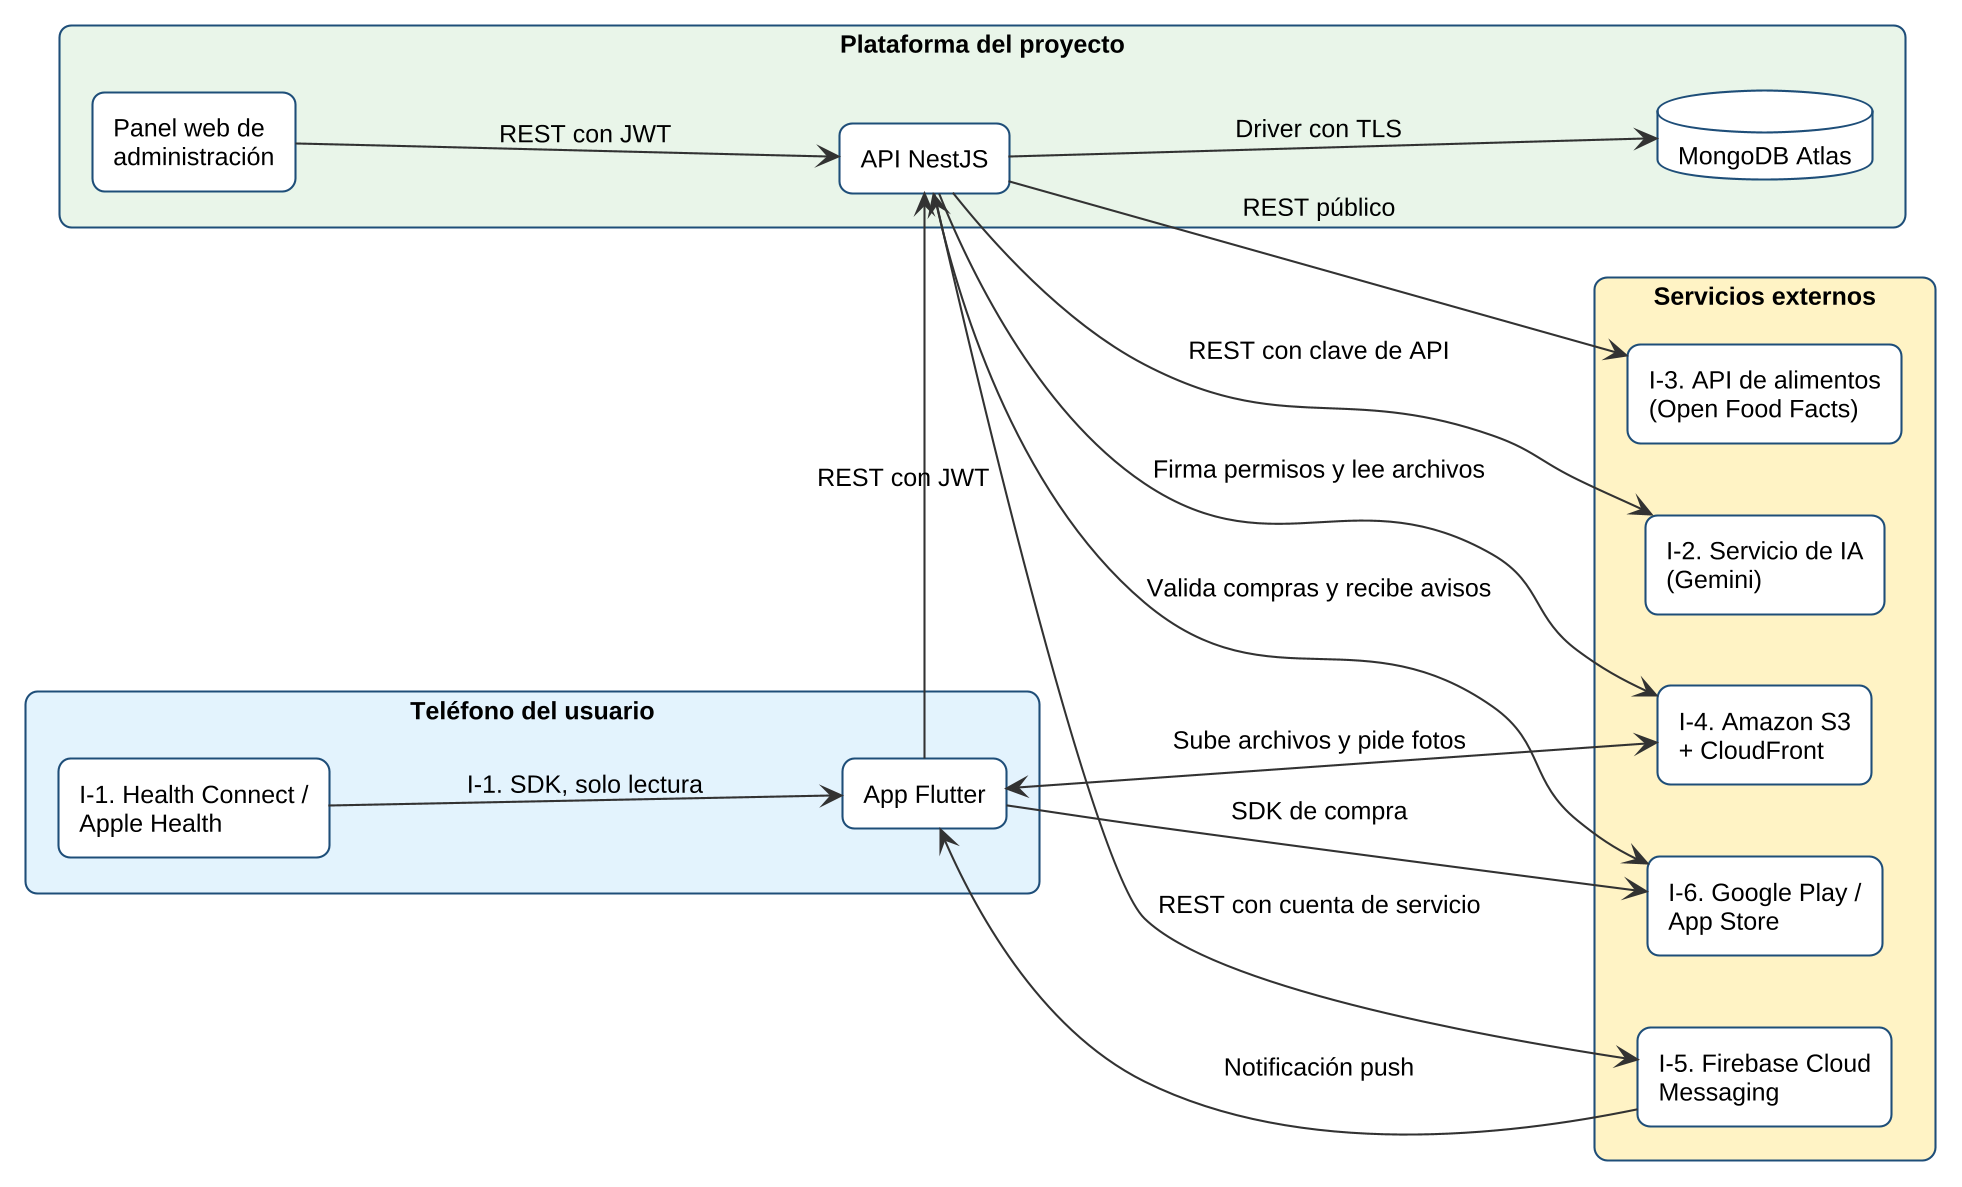
\includegraphics[width=1\textwidth,height=0.5\textheight,keepaspectratio]{figuras/arquitectura/diagrama_integraciones.png}
    \captionof{figure}{Diagrama general de integraciones.}
    \label{fig:diagrama_integraciones}
\end{center}

La Tabla \ref{tab:integraciones} resume cada integración y lo que ocurre cuando el sistema externo falla. Ninguna falla externa debería impedir que el usuario siga registrando sus datos a mano.

\begin{table}[h!]
    \centering
    \renewcommand{\arraystretch}{1.25}
    \footnotesize
    \begin{tabular}{|p{0.7cm}|>{\raggedright\arraybackslash}p{2.6cm}|>{\raggedright\arraybackslash}p{3.8cm}|>{\raggedright\arraybackslash}p{3.3cm}|>{\raggedright\arraybackslash}p{3.8cm}|}
        \hline
        \rowcolor[HTML]{EFEFEF}
        \textbf{ID} & \textbf{Sistema} & \textbf{Para qué se usa} & \textbf{Cómo se conecta} & \textbf{Si falla} \\ \hline
        I-1 & Health Connect y Apple Health & Leer las sesiones de cardio del reloj (CU-03, CU-21) & SDK en el teléfono, solo lectura, con permiso del usuario & La sesión se puede registrar con el GPS o a mano (CU-17) \\ \hline
        I-2 & Servicio de IA (Gemini) & Entender fotos de comida y textos (CU-02, CU-07, CU-16) & REST desde el backend, con clave de API & Se ofrece el registro manual (CU-01 y CU-06) \\ \hline
        I-3 & API de alimentos (Open Food Facts) & Buscar productos por código de barras (CU-15) & REST público desde el backend & Se ofrece buscar el alimento en la lista (CU-06) \\ \hline
        I-4 & Amazon S3 y CloudFront & Guardar y mostrar fotos y archivos \texttt{.fit} (CU-04, CU-09, CU-23) & Subida con URL prefirmada y lectura por CloudFront & Se avisa al usuario y se conserva lo escrito para reintentar \\ \hline
        I-5 & Firebase Cloud Messaging & Enviar alertas de fatiga al teléfono (CU-05) & REST desde el backend, con cuenta de servicio & La alerta queda visible en el resumen de la aplicación \\ \hline
        I-6 & Google Play y App Store & Cobrar y cancelar la suscripción (CU-24, CU-25) & SDK de compra en el teléfono y API de la tienda en el backend & No se activa el plan premium hasta confirmar el pago \\ \hline
    \end{tabular}
    \caption{Resumen de las integraciones con sistemas externos.}
    \label{tab:integraciones}
\end{table}
A continuación se presenta el diseño de cada integración, indicando los datos que se envían y se reciben en cada mensaje.
\vspace{0.4cm}

\noindent\begin{minipage}{\linewidth}
\textbf{I-1. Health Connect y Apple Health}

La Figura \ref{fig:int_salud} muestra la lectura de las sesiones que registró el reloj.
\begin{center}
    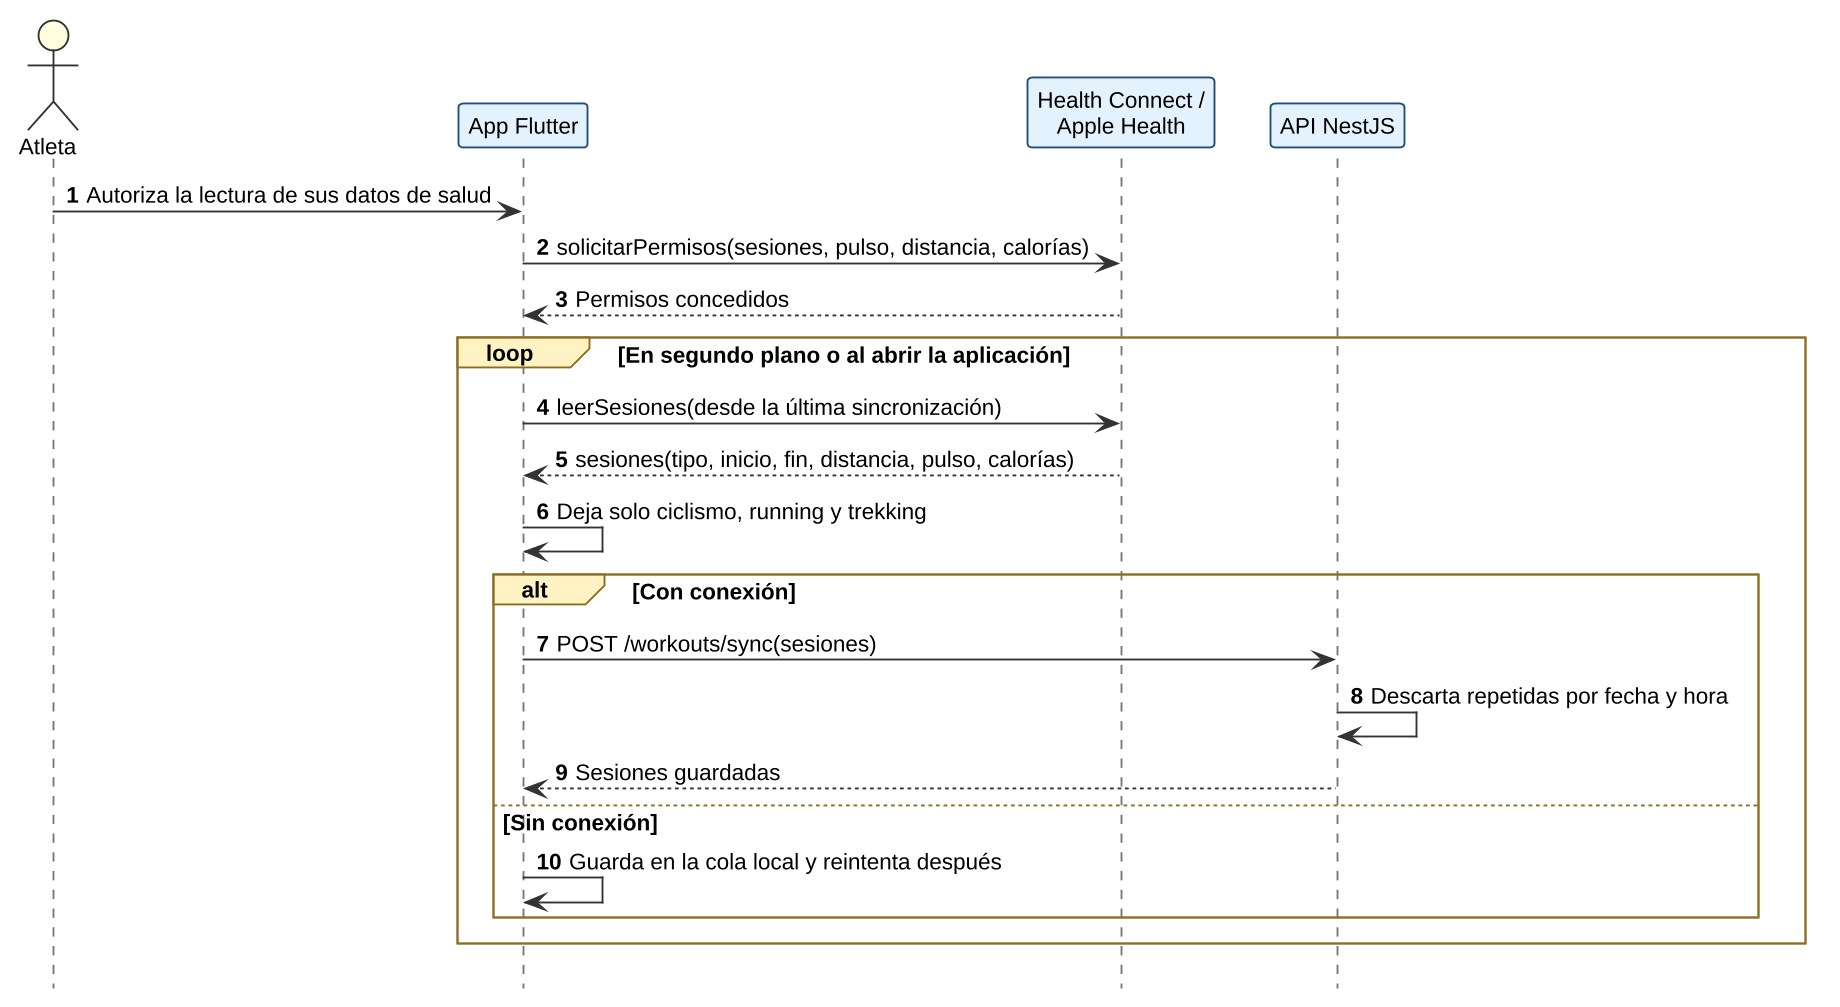
\includegraphics[width=0.95\textwidth,height=0.5\textheight,keepaspectratio]{figuras/secuencia/int_salud.png}
    \captionof{figure}{Integración I-1: Health Connect y Apple Health.}
    \label{fig:int_salud}
\end{center}
Estos servicios funcionan dentro del teléfono y no tienen una conexión directa con el servidor, por lo que la lectura la hace la aplicación con sus SDK. Solo se pide permiso para los datos necesarios, y el usuario puede retirarlo cuando quiera (CU-21). La integración es solo de lectura. Si no hay conexión, las sesiones esperan en una cola local. El backend descarta las repetidas según su fecha y hora, y conserva la versión con más detalle si la misma sesión llegó en un archivo \texttt{.fit}.
\end{minipage}
\vspace{0.6cm}

\noindent\begin{minipage}{\linewidth}
\textbf{I-2. Servicio de inteligencia artificial}

La Figura \ref{fig:int_ia} muestra cómo se estima una comida a partir de una foto o de un texto. El registro de fuerza por lenguaje natural usa el mismo esquema.
\begin{center}
    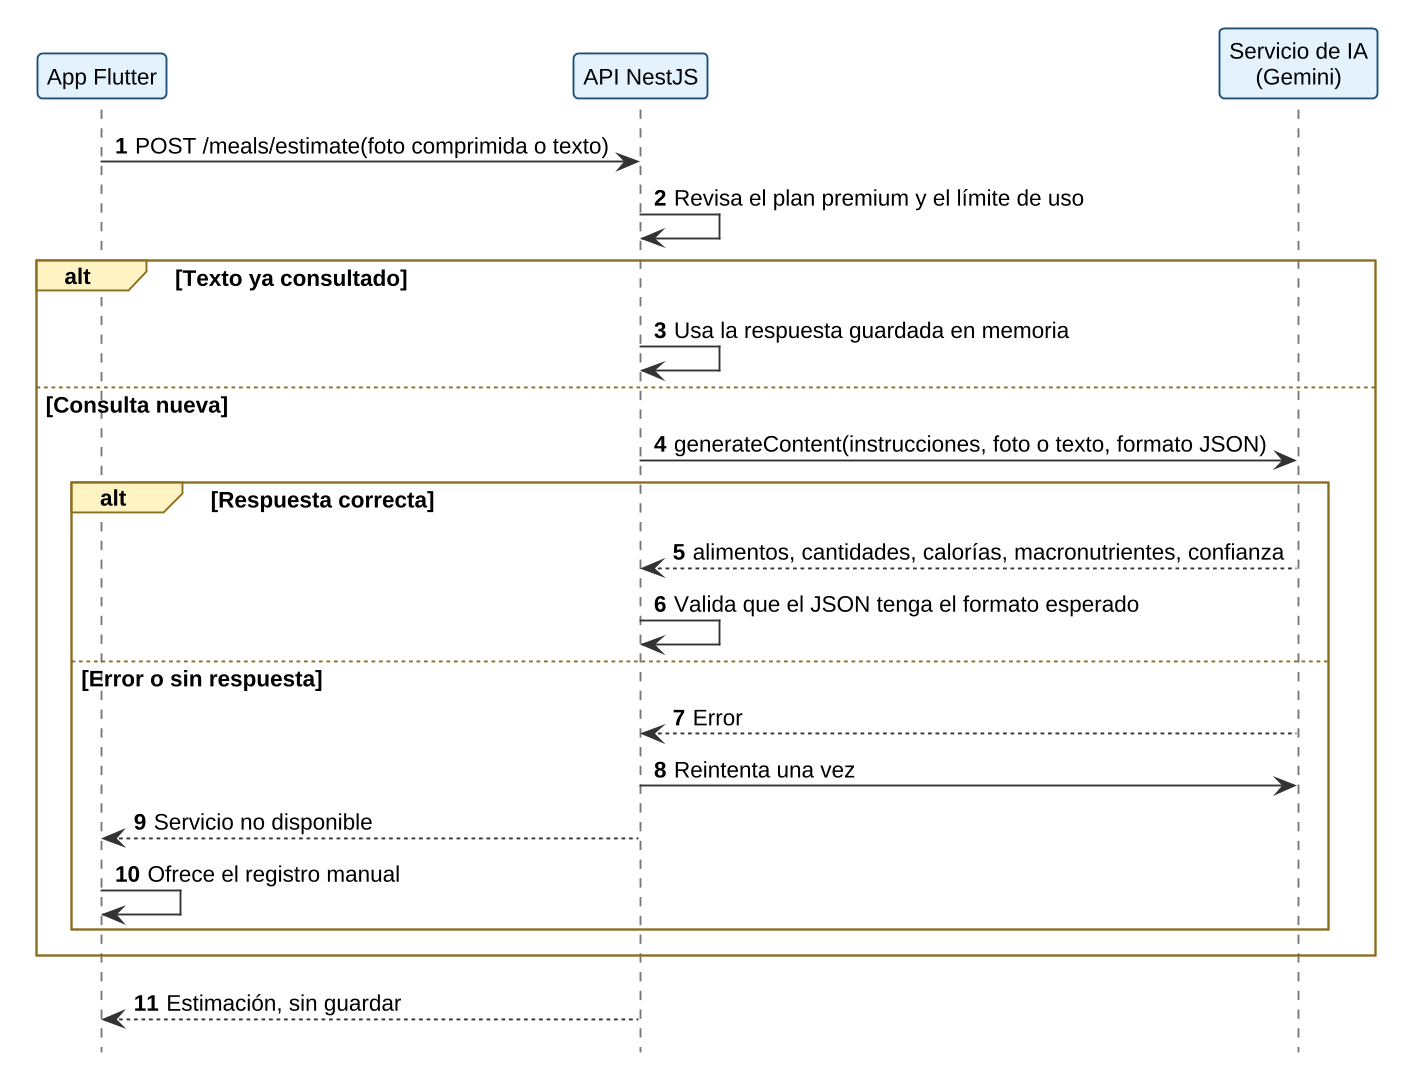
\includegraphics[width=0.95\textwidth,height=0.5\textheight,keepaspectratio]{figuras/secuencia/int_ia.png}
    \captionof{figure}{Integración I-2: Servicio de inteligencia artificial.}
    \label{fig:int_ia}
\end{center}
La aplicación nunca llama directamente al servicio de IA, para no exponer la clave y para poder controlar el gasto. El backend revisa primero el plan del usuario y su límite de uso. Solo envía la foto o el texto, sin datos que identifiquen a la persona. Como la respuesta viene de un modelo, el backend valida que el JSON tenga el formato esperado, y el usuario siempre revisa el resultado antes de guardarlo. Si se quisiera cambiar de proveedor, solo cambiaría esta integración.
\end{minipage}
\vspace{0.6cm}

\noindent\begin{minipage}{\linewidth}
\textbf{I-3. API de alimentos}

La Figura \ref{fig:int_alimentos} muestra la búsqueda de un producto por su código de barras.
\begin{center}
    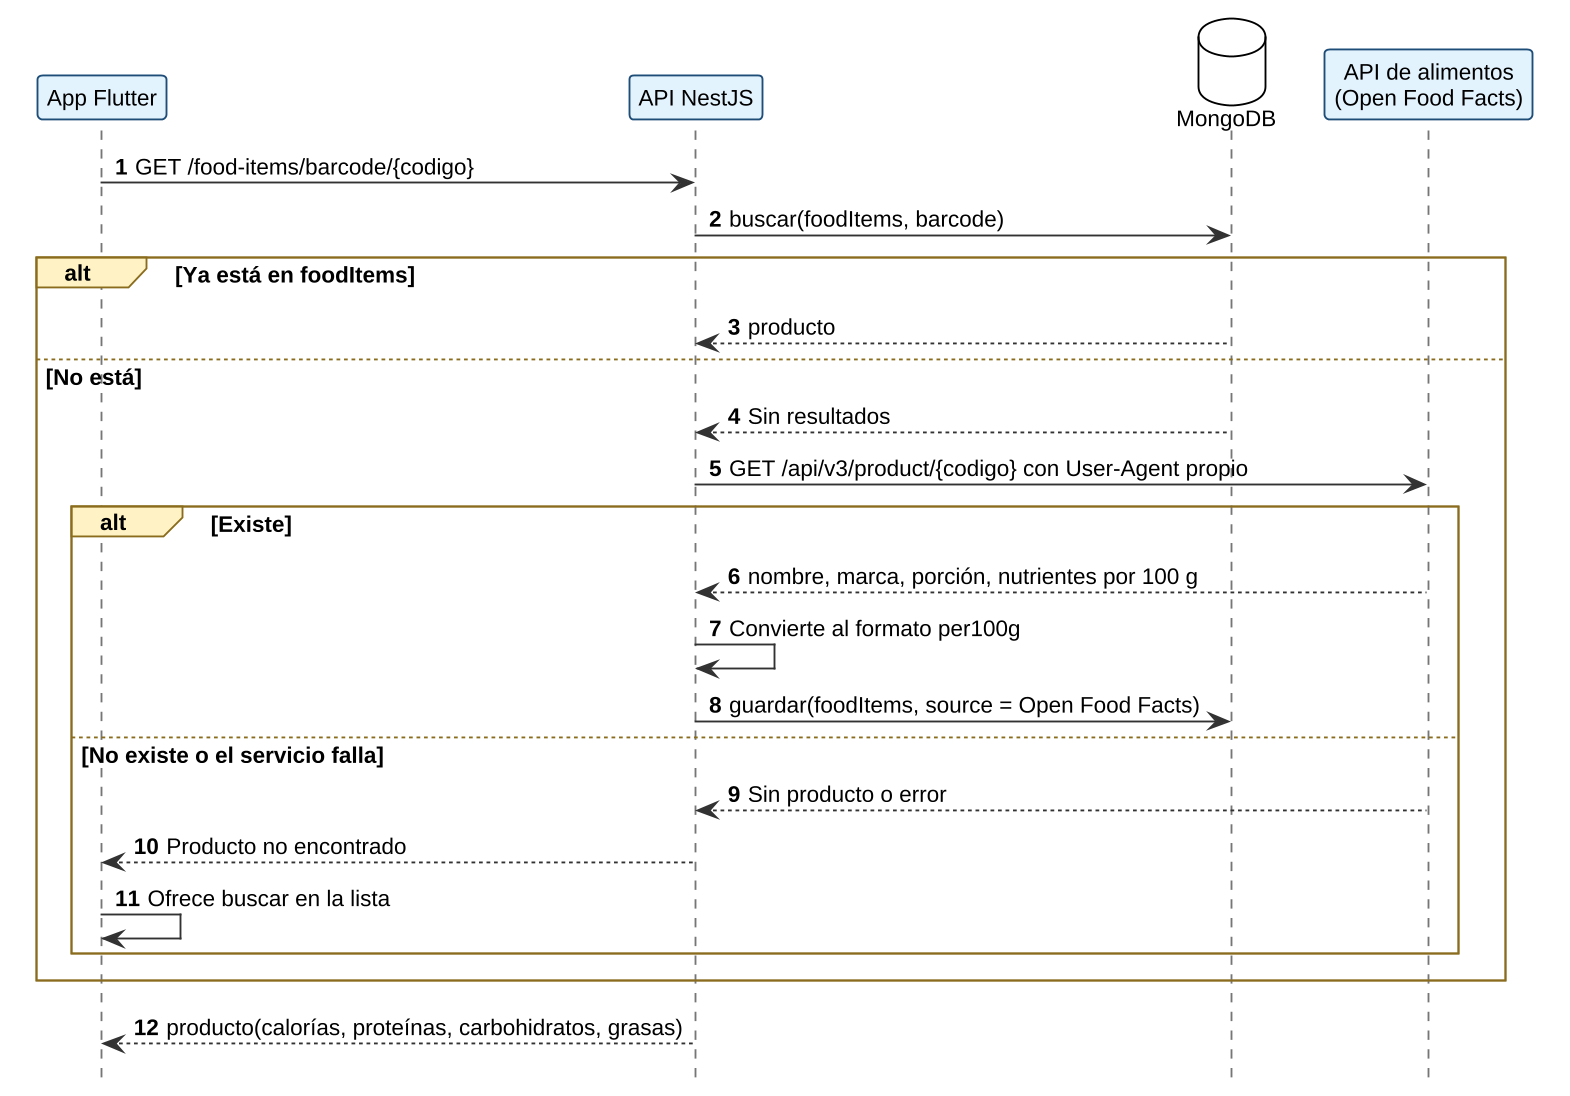
\includegraphics[width=0.95\textwidth,height=0.5\textheight,keepaspectratio]{figuras/secuencia/int_alimentos.png}
    \captionof{figure}{Integración I-3: API de alimentos.}
    \label{fig:int_alimentos}
\end{center}
Se usa la API de Open Food Facts, que para leer datos no pide autenticación, pero sí un identificador propio de la aplicación en cada consulta \citep{off_api}. Cada producto encontrado se guarda en \texttt{foodItems}, para que la siguiente consulta sea más rápida y no dependa del servicio. La licencia de estos datos (ODbL) exige indicar su origen y compartir en las mismas condiciones las bases de datos derivadas \citep{off_api}. Por eso cada producto queda marcado con su fuente en el campo \texttt{source} y la aplicación mostrará la atribución.
\end{minipage}
\vspace{0.6cm}

\noindent\begin{minipage}{\linewidth}
\textbf{I-4. Almacenamiento de archivos}

La Figura \ref{fig:int_archivos} muestra cómo se suben y se muestran las fotos de una publicación.
\begin{center}
    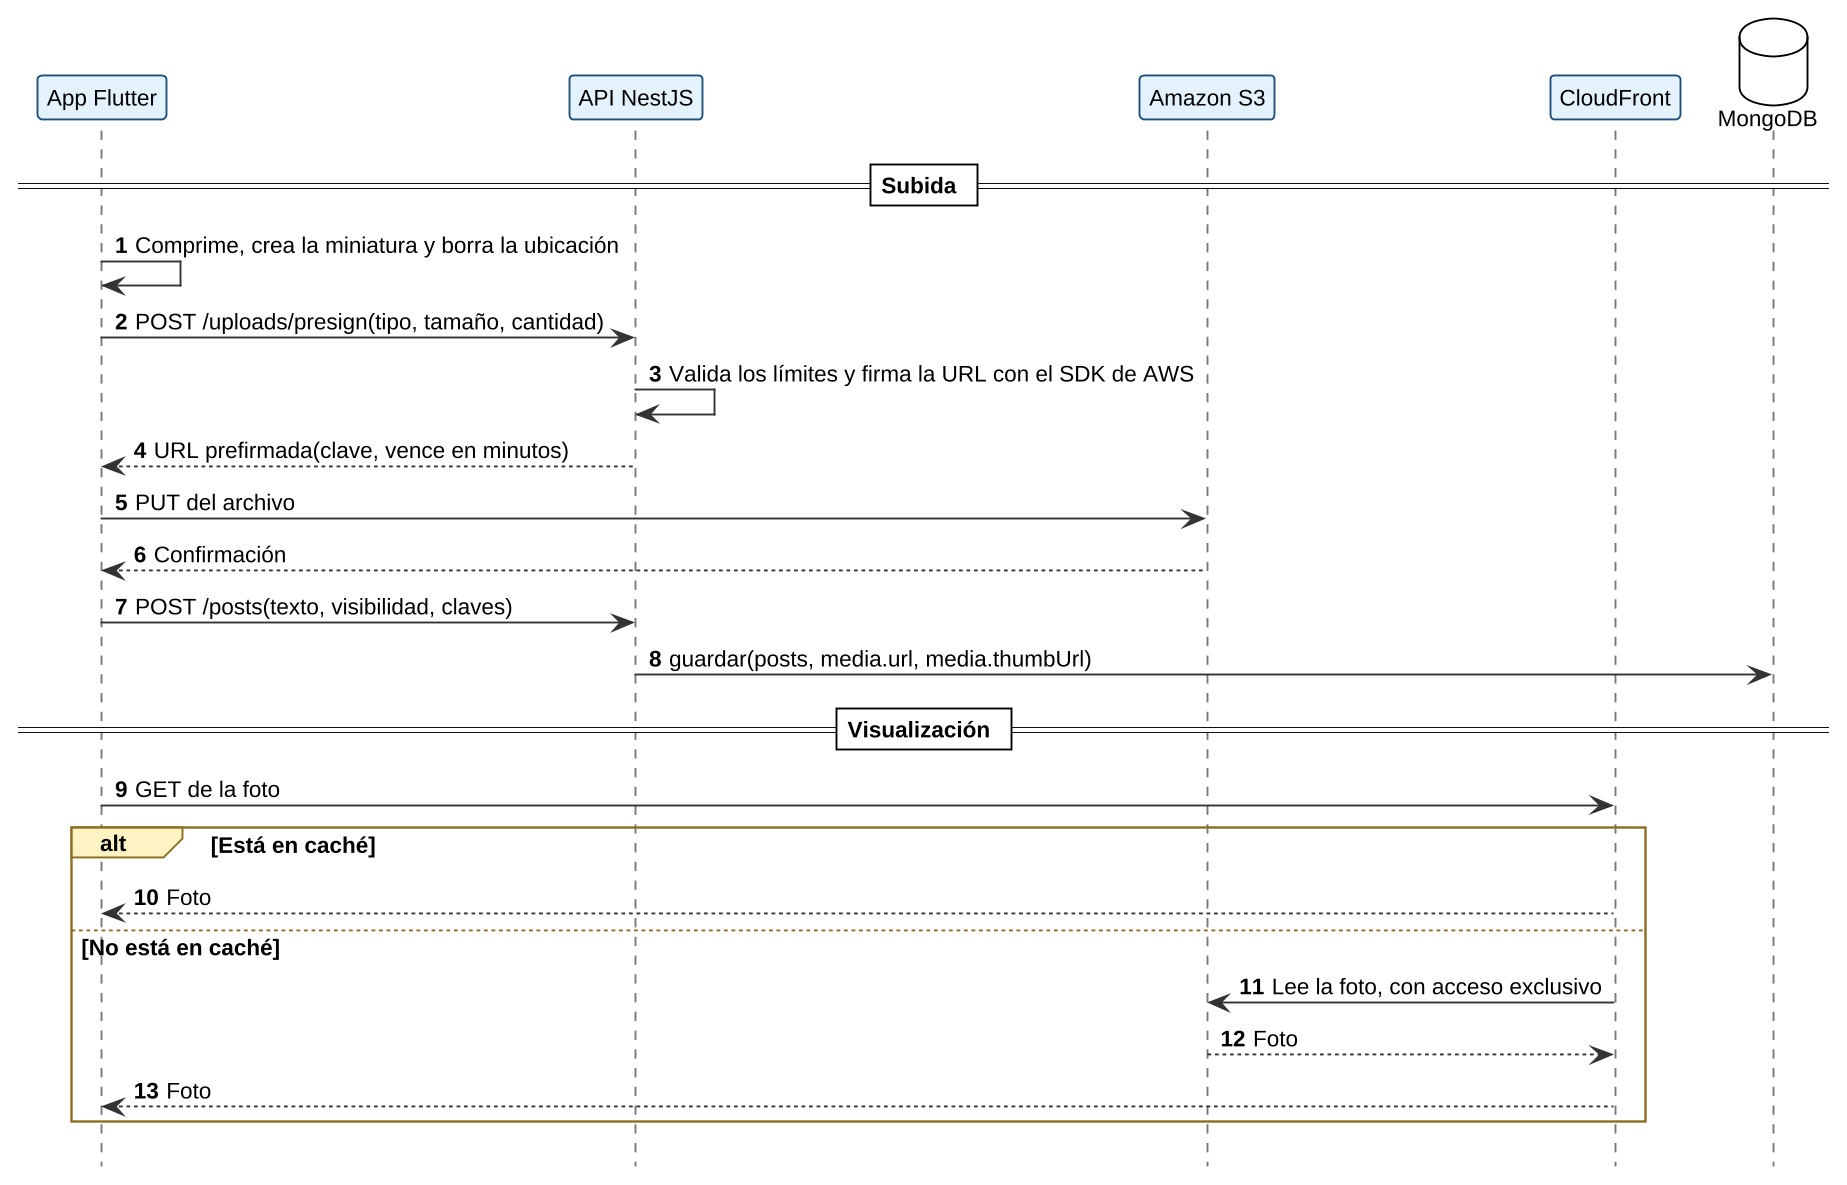
\includegraphics[width=0.95\textwidth,height=0.5\textheight,keepaspectratio]{figuras/secuencia/int_archivos.png}
    \captionof{figure}{Integración I-4: Almacenamiento de archivos.}
    \label{fig:int_archivos}
\end{center}
El teléfono sube los archivos directamente a Amazon S3 con una URL prefirmada, que vence en pocos minutos y sirve solo para ese archivo. Firmar la URL no requiere una llamada a S3, porque el backend lo hace con sus credenciales. Las fotos se muestran a través de CloudFront, que es el único servicio con permiso para leer el bucket. Los archivos \texttt{.fit} se suben igual, pero no pasan por CloudFront, porque solo los lee el backend (CU-04).
\end{minipage}
\vspace{0.6cm}

\noindent\begin{minipage}{\linewidth}
\textbf{I-5. Notificaciones}

La Figura \ref{fig:int_notificaciones} muestra el registro del teléfono y el envío de una alerta.
\begin{center}
    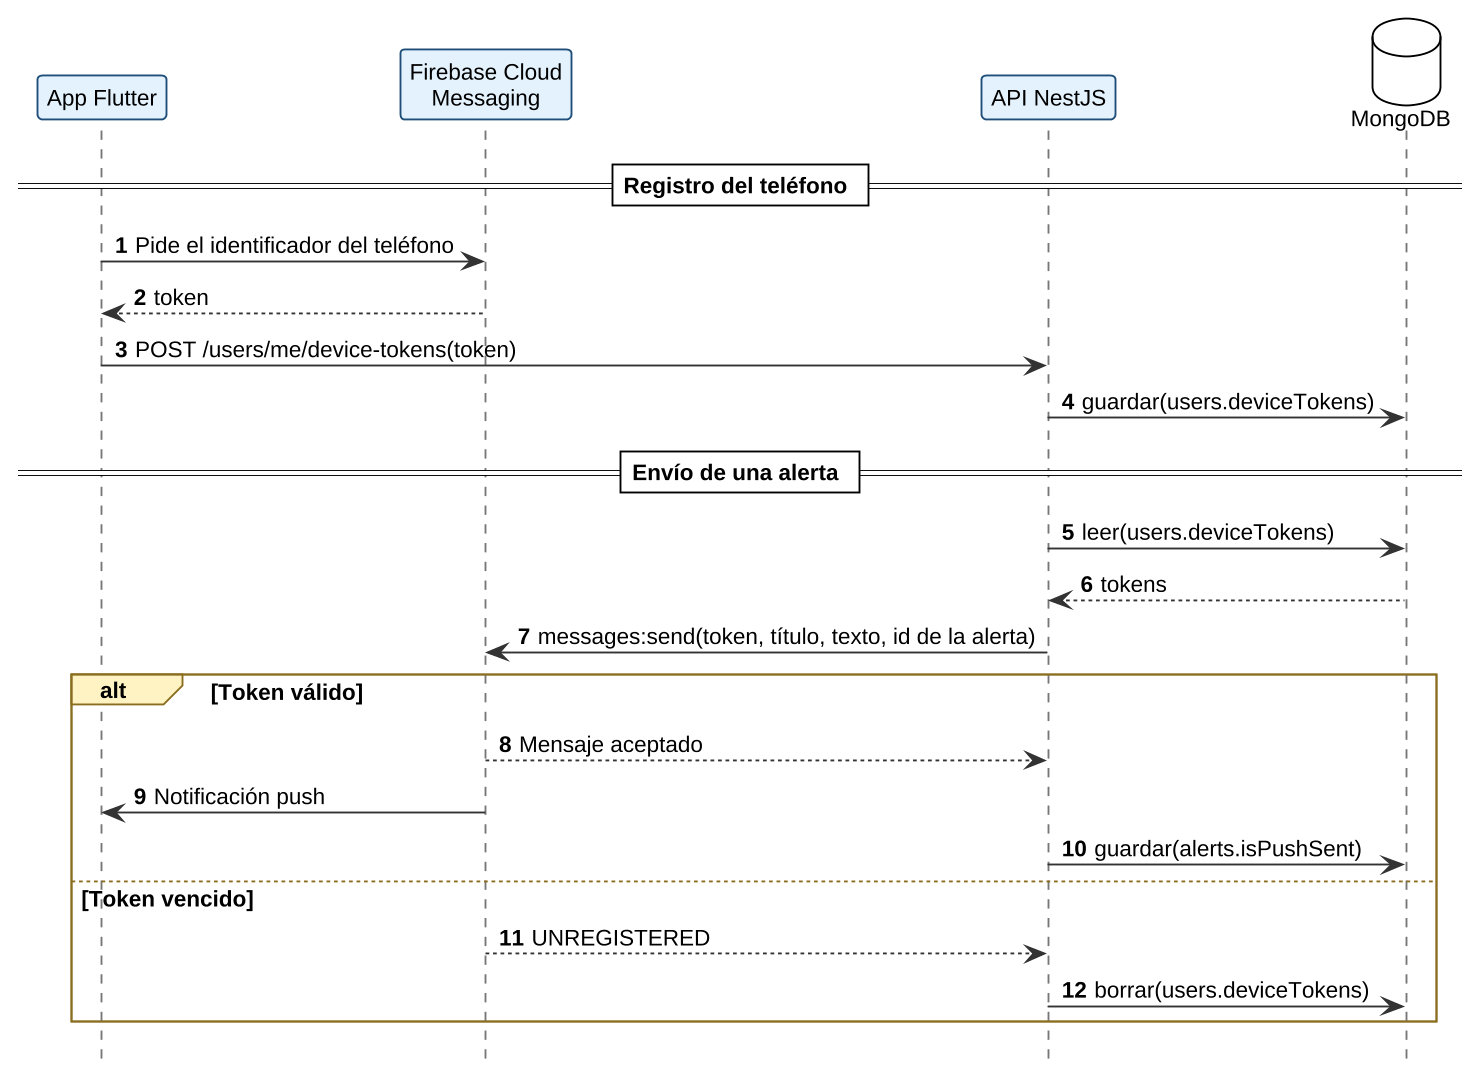
\includegraphics[width=0.95\textwidth,height=0.5\textheight,keepaspectratio]{figuras/secuencia/int_notificaciones.png}
    \captionof{figure}{Integración I-5: Notificaciones.}
    \label{fig:int_notificaciones}
\end{center}
Para enviar una notificación se necesita el identificador del teléfono, que la aplicación obtiene de Firebase y entrega al backend. Un usuario puede tener más de un teléfono, por lo que se guarda en la lista \texttt{deviceTokens}. Si Firebase responde que un identificador ya no sirve, el backend lo borra. La notificación solo es un aviso, ya que la alerta queda guardada en \texttt{fatigueSnapshots}. Así, el usuario puede verla aunque la notificación no le llegue.
\end{minipage}
\vspace{0.6cm}

\noindent\begin{minipage}{\linewidth}
\textbf{I-6. Google Play y App Store}

La Figura \ref{fig:int_pagos} muestra la compra de la suscripción y sus cambios posteriores.
\begin{center}
    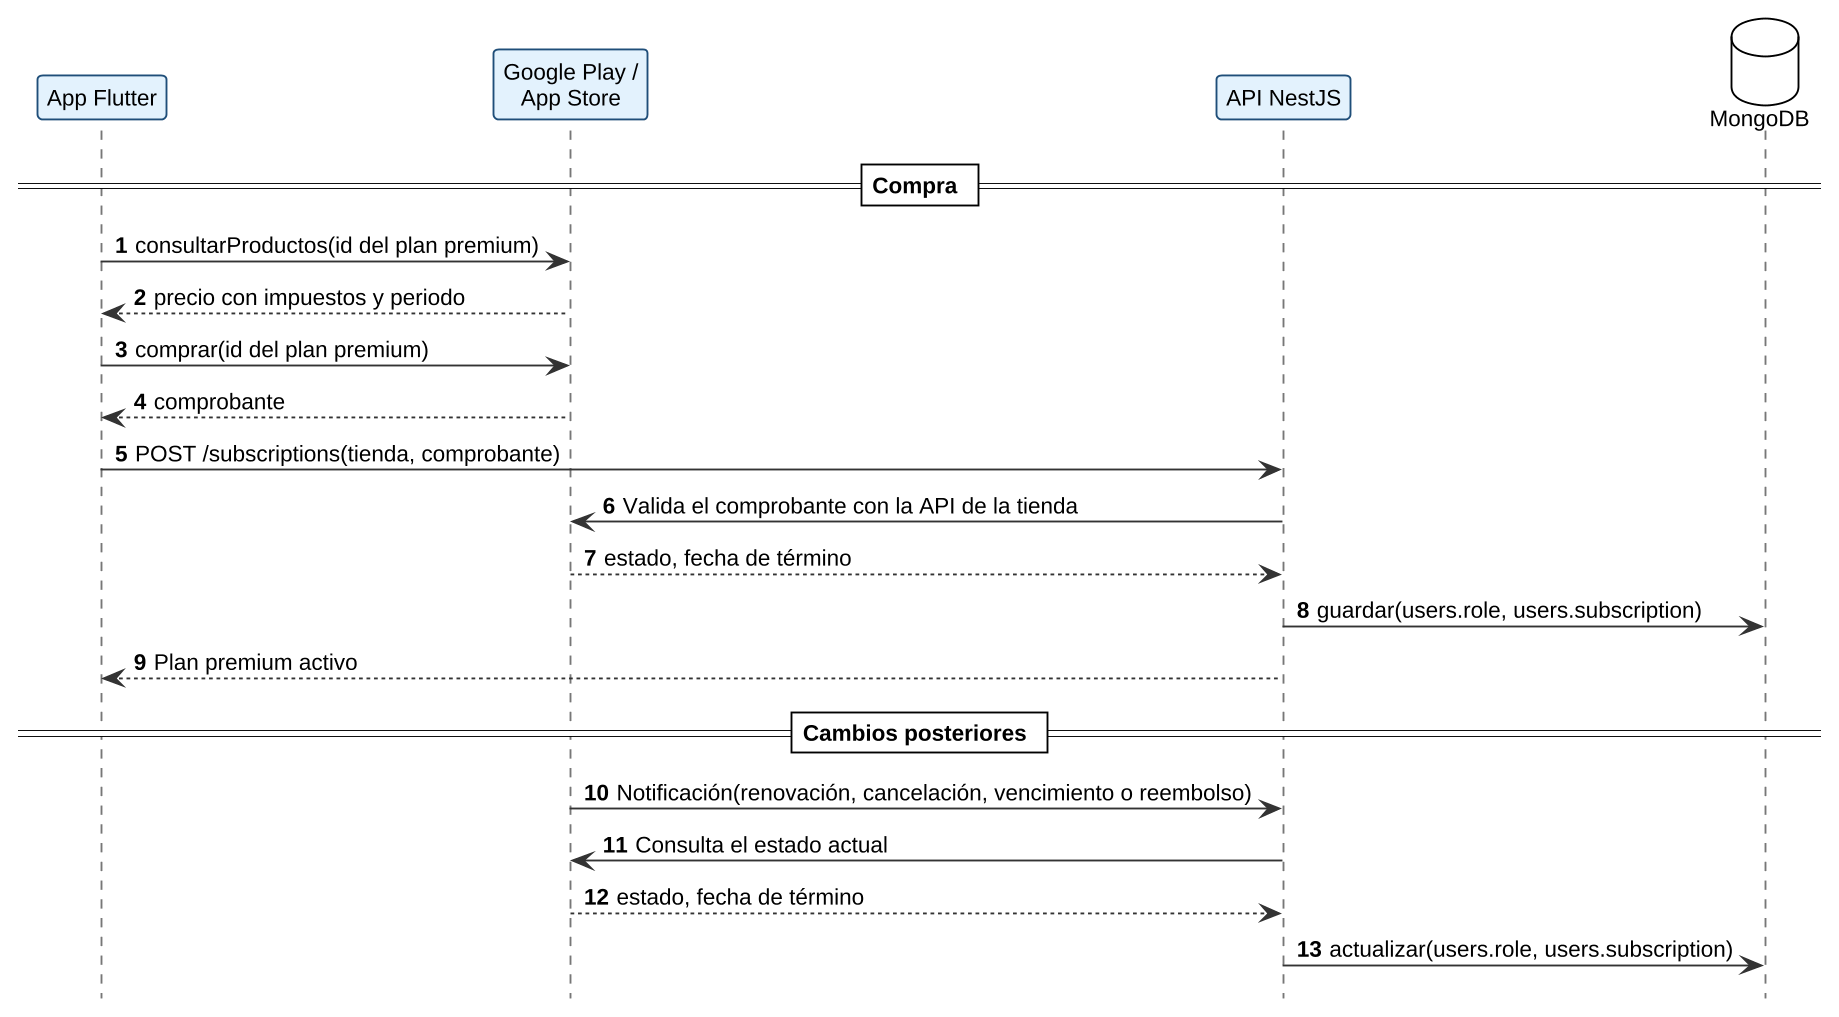
\includegraphics[width=0.95\textwidth,height=0.5\textheight,keepaspectratio]{figuras/secuencia/int_pagos.png}
    \captionof{figure}{Integración I-6: Google Play y App Store.}
    \label{fig:int_pagos}
\end{center}
El pago se hace completo en la tienda, por lo que el sistema nunca recibe los datos de la tarjeta. El backend no confía solo en lo que informa la aplicación, sino que valida cada comprobante con la API de la tienda antes de activar el plan. Las renovaciones, cancelaciones y reembolsos ocurren fuera de la aplicación, así que la tienda avisa al backend. Como ese aviso solo indica que algo cambió, el backend consulta después el estado actual \citep{google_play_rtdn}.
\end{minipage}
\vspace{0.6cm}

\subsection{Dimensionamiento y Arquitectura Detallada de la Solución}
Esta sección indica qué infraestructura se necesita para operar el MVP y cuánta capacidad debe tener. El cálculo usa como base los 1.500 usuarios del mercado objetivo inicial. La Figura \ref{fig:arquitectura_detallada} muestra la arquitectura.
\begin{center}
    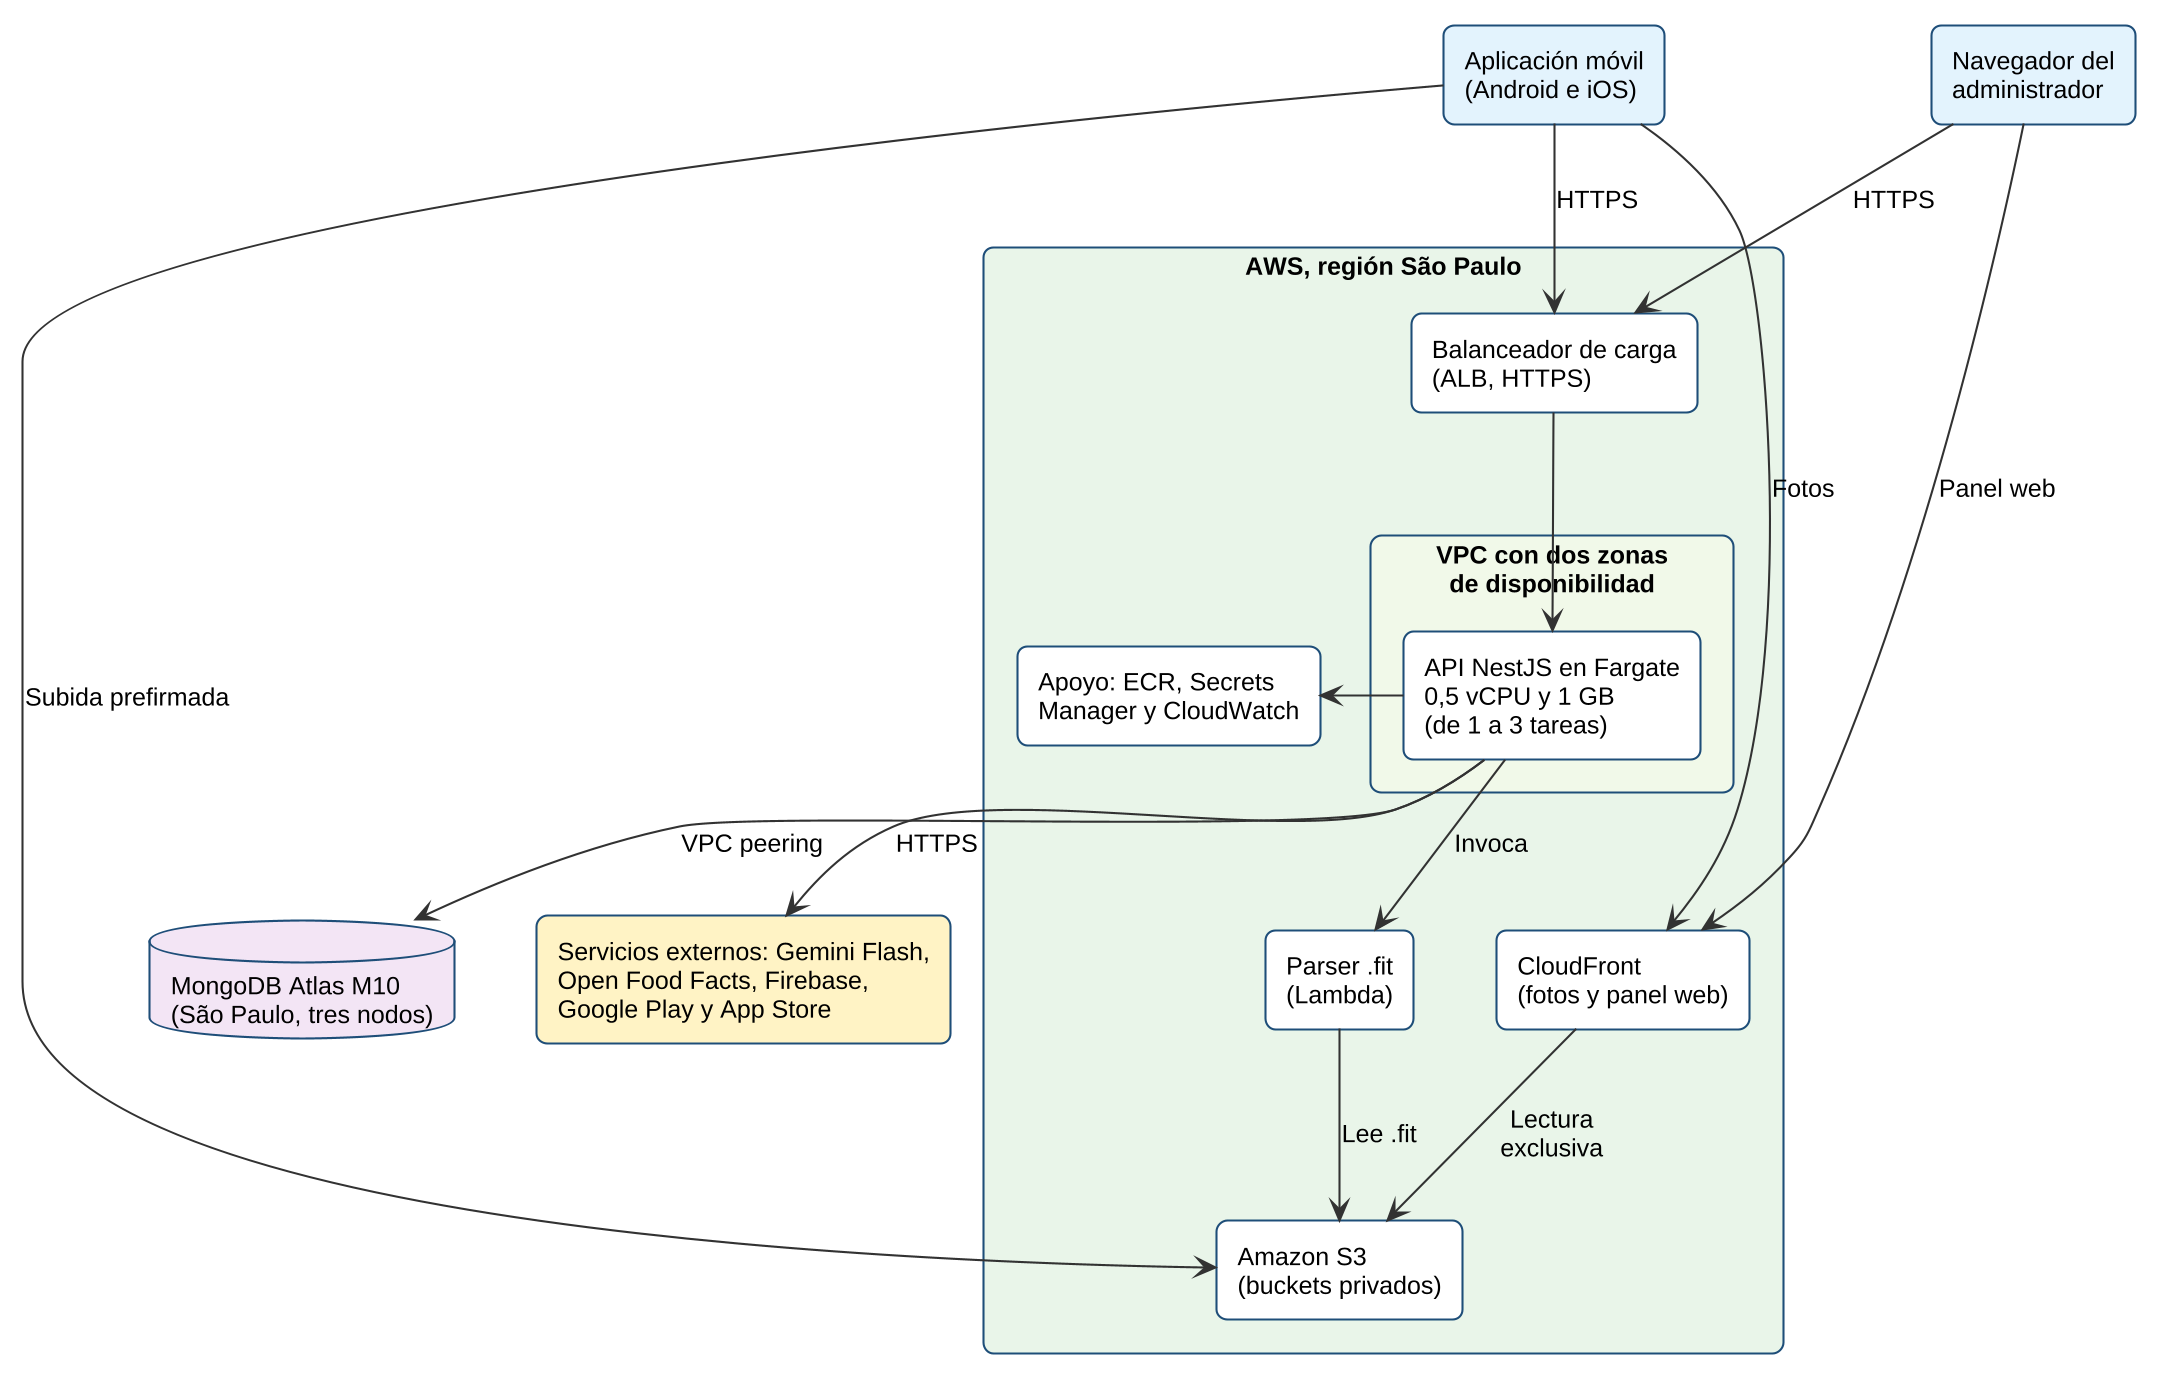
\includegraphics[width=0.95\textwidth,height=0.5\textheight,keepaspectratio]{figuras/arquitectura/arquitectura_detallada.png}
    \captionof{figure}{Arquitectura detallada de la solución.}
    \label{fig:arquitectura_detallada}
\end{center}

Las principales decisiones de esta arquitectura son las siguientes:

\begin{itemize}
    \item \textbf{Región de São Paulo:} Es la región de AWS más cercana con todos estos servicios, lo que reduce el tiempo de respuesta para usuarios en Chile. La base de datos está en la misma región.
    \item \textbf{API en Fargate:} Un contenedor pequeño alcanza para la carga esperada, y se agregan más cuando aumenta el uso. Para evitar el costo de una NAT Gateway, las tareas usan una IP pública, pero sus reglas de red solo aceptan tráfico entrante desde el balanceador.
    \item \textbf{Parser en Lambda:} Se esperan unos 20 archivos \texttt{.fit} al día, por lo que un contenedor encendido todo el tiempo estaría casi siempre sin hacer nada. Una función Lambda solo se ejecuta cuando llega un archivo.
    \item \textbf{MongoDB Atlas M10:} Es el nivel más bajo que permite una conexión privada con la red de AWS (VPC peering). Los datos de salud son sensibles, así que no conviene que la base de datos acepte conexiones desde cualquier dirección de Internet. Además, trae tres nodos con réplica y respaldos automáticos.
    \item \textbf{S3 y CloudFront:} Las fotos y los archivos no pasan por la API, como se explicó en la sección de integraciones.
\end{itemize}

\textbf{Carga esperada}

La Tabla \ref{tab:carga_esperada} muestra la carga estimada. Son supuestos que se deben confirmar con las pruebas de carga y con el uso real del prototipo.

\begin{table}[h!]
    \centering
    \renewcommand{\arraystretch}{1.25}
    \footnotesize
    \begin{tabular}{|>{\raggedright\arraybackslash}p{7.5cm}|>{\raggedright\arraybackslash}p{7.5cm}|}
        \hline
        \rowcolor[HTML]{EFEFEF}
        \textbf{Indicador} & \textbf{Valor estimado} \\ \hline
        Usuarios registrados & 1.500, de los cuales 159 son premium \\ \hline
        Usuarios activos al día & 600 (40\% de los registrados) \\ \hline
        Llamadas a la API al día & 24.000 (40 por usuario activo) \\ \hline
        Hora de mayor uso & 7.200 llamadas, 30\% del total del día \\ \hline
        Llamadas por segundo & 2 en promedio en la hora de mayor uso, y hasta 10 en momentos puntuales \\ \hline
        Archivos \texttt{.fit} al día & 20 (30\% de los premium, con 3 archivos a la semana) \\ \hline
        Fotos nuevas al mes & 7.200 (Tabla \ref{tab:costo_imagenes}) \\ \hline
    \end{tabular}
    \caption{Carga esperada del sistema.}
    \label{tab:carga_esperada}
\end{table}

\textbf{Almacenamiento}

La Tabla \ref{tab:almacenamiento} estima el espacio que usará MongoDB al cuarto año. La colección más grande es \texttt{telemetry}. Se asume que sus puntos ocupan 60 bytes cada uno y que las colecciones de series temporales de MongoDB los comprimen en un 70\%. Este último valor es un supuesto que se debe medir con datos reales.

\begin{table}[h!]
    \centering
    \renewcommand{\arraystretch}{1.25}
    \footnotesize
    \begin{tabular}{|>{\raggedright\arraybackslash}p{4cm}|r|>{\raggedright\arraybackslash}p{5.5cm}|r|}
        \hline
        \rowcolor[HTML]{EFEFEF}
        \textbf{Colección} & \textbf{Documentos} & \textbf{Cómo se calcula} & \textbf{Espacio} \\ \hline
        \texttt{telemetry} & 529 millones de puntos & Archivos \texttt{.fit} (1,5 horas, un punto por segundo) y rutas con GPS (1 hora, un punto cada 5 segundos) & 8,9 GB \\ \hline
        \texttt{meals} & 2,6 millones & 600 usuarios con 3 comidas al día, a 1,5 KB & 3,8 GB \\ \hline
        \texttt{workouts} & 499 mil & 600 usuarios con 4 sesiones a la semana, a 3 KB & 1,4 GB \\ \hline
        \texttt{dailyLogs} & 877 mil & 600 usuarios con un documento al día, a 1 KB & 0,8 GB \\ \hline
        \texttt{posts} y \texttt{fatigueSnapshots} & 405 mil & 3.600 publicaciones al mes y un cálculo diario por usuario premium & 0,5 GB \\ \hline
        Otras colecciones &  & Catálogos, rutinas, rutas, recetas y usuarios & 0,5 GB \\ \hline
        Índices &  & 25\% adicional sobre lo anterior & 4,0 GB \\ \hline
        \rowcolor[HTML]{E8F5E9}
        \textbf{Total} &  &  & \textbf{19,9 GB} \\ \hline
    \end{tabular}
    \caption{Almacenamiento estimado en MongoDB al cuarto año.}
    \label{tab:almacenamiento}
\end{table}

El primer año se usarían cerca de 5 GB, por lo que los 10 GB iniciales de un clúster M10 alcanzan durante los primeros dos años. Después, el almacenamiento se puede ampliar sin cambiar de nivel, ya que M10 permite hasta 128 GB \citep{atlas_pricing}. En Amazon S3 se acumularían unos 118 GB de fotos (Tabla \ref{tab:costo_imagenes}) y 29 GB de archivos \texttt{.fit} al cuarto año.
\textbf{Dimensionamiento por ambiente}

La Tabla \ref{tab:ambientes} muestra los recursos de cada ambiente. Como una sola persona desarrolla el proyecto, se usan tres ambientes simples. Los datos de prueba nunca se mezclan con los de producción.

\begin{table}[h!]
    \centering
    \renewcommand{\arraystretch}{1.25}
    \footnotesize
    \begin{tabular}{|>{\raggedright\arraybackslash}p{1.9cm}|>{\raggedright\arraybackslash}p{3.3cm}|>{\raggedright\arraybackslash}p{2.9cm}|>{\raggedright\arraybackslash}p{3.2cm}|>{\raggedright\arraybackslash}p{2.9cm}|}
        \hline
        \rowcolor[HTML]{EFEFEF}
        \textbf{Ambiente} & \textbf{Componente} & \textbf{Servicio} & \textbf{Capacidad} & \textbf{Observación} \\ \hline
        Producción & API & AWS Fargate & 0,5 vCPU y 1 GB, de 1 a 3 tareas & Agrega tareas si la CPU supera el 60\% \\ \hline
        Producción & Parser \texttt{.fit} & AWS Lambda & 1.769 MB de memoria & Se ejecuta solo al recibir un archivo \\ \hline
        Producción & Base de datos & MongoDB Atlas M10 & 2 vCPU, 2 GB de RAM y 10 GB, ampliable & Tres nodos con réplica \\ \hline
        Producción & Archivos y fotos & S3 y CloudFront & 118 GB de fotos y 29 GB de \texttt{.fit} al cuarto año & Buckets privados \\ \hline
        Producción & Balanceador & ALB & Dos zonas de disponibilidad & Certificado HTTPS \\ \hline
        QA & API & AWS Fargate & 0,25 vCPU y 0,5 GB, 1 tarea & Se enciende solo durante las pruebas \\ \hline
        QA & Base de datos & MongoDB Atlas M0 & 512 MB & Nivel gratuito, sin datos reales \\ \hline
        QA & Aplicación & Prueba interna de Google Play y TestFlight & Unos pocos usuarios & Evaluaciones del prototipo \\ \hline
        Desarrollo & API y base de datos & Docker en el computador & Según el computador & Sin costo de nube \\ \hline
        Desarrollo & Aplicación & Emulador o teléfono de prueba &  & Sin costo de nube \\ \hline
    \end{tabular}
    \caption{Dimensionamiento por ambiente.}
    \label{tab:ambientes}
\end{table}

La API se dimensionó con una tarea, porque la carga esperada es baja. Si esa tarea falla, AWS la reemplaza automáticamente, aunque el servicio puede quedar interrumpido por uno o dos minutos. Tener dos tareas permanentes evitaría esa interrupción, pero duplicaría el costo de este componente. Por eso se deja como una mejora para cuando la cantidad de usuarios lo justifique.
\textbf{Costo mensual de producción}

La Tabla \ref{tab:costo_produccion} muestra el costo de este dimensionamiento. Los precios de AWS son los publicados para la región de São Paulo \citep{aws_fargate_pricing}. MongoDB publica un valor de USD 57 al mes para M10 en Virginia \citep{atlas_pricing}, pero no se pudo confirmar el valor en São Paulo. Como los servicios de AWS cuestan cerca de un 70\% más en esa región, se considera USD 100 al mes, incluidos el almacenamiento y los respaldos. Este valor se debe confirmar antes de contratar el servicio.

\begin{table}[h!]
    \centering
    \renewcommand{\arraystretch}{1.25}
    \footnotesize
    \begin{tabular}{|>{\raggedright\arraybackslash}p{5cm}|>{\raggedright\arraybackslash}p{7.5cm}|r|}
        \hline
        \rowcolor[HTML]{EFEFEF}
        \textbf{Componente} & \textbf{Detalle} & \textbf{USD/mes} \\ \hline
        API en Fargate & 1 tarea de 0,5 vCPU y 1 GB, todo el mes & 31 \\ \hline
        Parser en Lambda & Dentro del nivel gratuito de AWS & 0 \\ \hline
        MongoDB Atlas M10 & Estimación para São Paulo & 100 \\ \hline
        Balanceador (ALB) & USD 0,034 por hora y uso bajo & 29 \\ \hline
        Direcciones IP públicas & 3 direcciones a USD 0,005 por hora & 11 \\ \hline
        CloudWatch & 5 GB de registros al mes & 5 \\ \hline
        S3 para archivos \texttt{.fit} & 29 GB al cuarto año, más solicitudes & 2 \\ \hline
        Fotos en S3 y CloudFront & Tabla \ref{tab:costo_imagenes} & 6 \\ \hline
        Secrets Manager, ECR y dominio & 6 secretos, 1 GB de imágenes y nombre de dominio & 4 \\ \hline
        \rowcolor[HTML]{E8F5E9}
        \textbf{Total} &  & \textbf{188} \\ \hline
    \end{tabular}
    \caption{Costo mensual estimado del ambiente de producción.}
    \label{tab:costo_produccion}
\end{table}

Este total es el que se usa en la factibilidad económica, donde corresponde a USD 182 al mes de infraestructura (Tabla \ref{tab:costo_infra}) y USD 6 al mes de imágenes (Tabla \ref{tab:costo_imagenes}). Con estos costos, y después de descontar el IVA, la comisión de las tiendas y el impuesto a la renta, la Alternativa 3 necesita 159 suscriptores para alcanzar el equilibrio.
\textbf{Cuándo aumentar la capacidad}

La Tabla \ref{tab:escalamiento} indica qué señal avisa que se debe ampliar cada componente.

\begin{table}[h!]
    \centering
    \renewcommand{\arraystretch}{1.25}
    \footnotesize
    \begin{tabular}{|>{\raggedright\arraybackslash}p{3.5cm}|>{\raggedright\arraybackslash}p{5.7cm}|>{\raggedright\arraybackslash}p{5.7cm}|}
        \hline
        \rowcolor[HTML]{EFEFEF}
        \textbf{Componente} & \textbf{Señal} & \textbf{Acción} \\ \hline
        API & La CPU supera el 60\% durante varios minutos & Agregar tareas automáticamente, hasta 3. Si no alcanza, subir la capacidad de cada tarea \\ \hline
        Base de datos & La memoria o la CPU se mantienen altas & Pasar de M10 a M20 \\ \hline
        Almacenamiento & Se usa más del 80\% del espacio & Ampliar el disco del clúster \\ \hline
        Entrega de fotos & Se acerca a 1 TB al mes & Pagar el exceso sobre el nivel gratuito de CloudFront \\ \hline
    \end{tabular}
    \caption{Señales para aumentar la capacidad.}
    \label{tab:escalamiento}
\end{table}
\subsection{Diagrama de Despliegue}
La Figura \ref{fig:diagrama_despliegue} muestra dónde se instala cada parte del sistema y cómo se comunican.
\begin{center}
    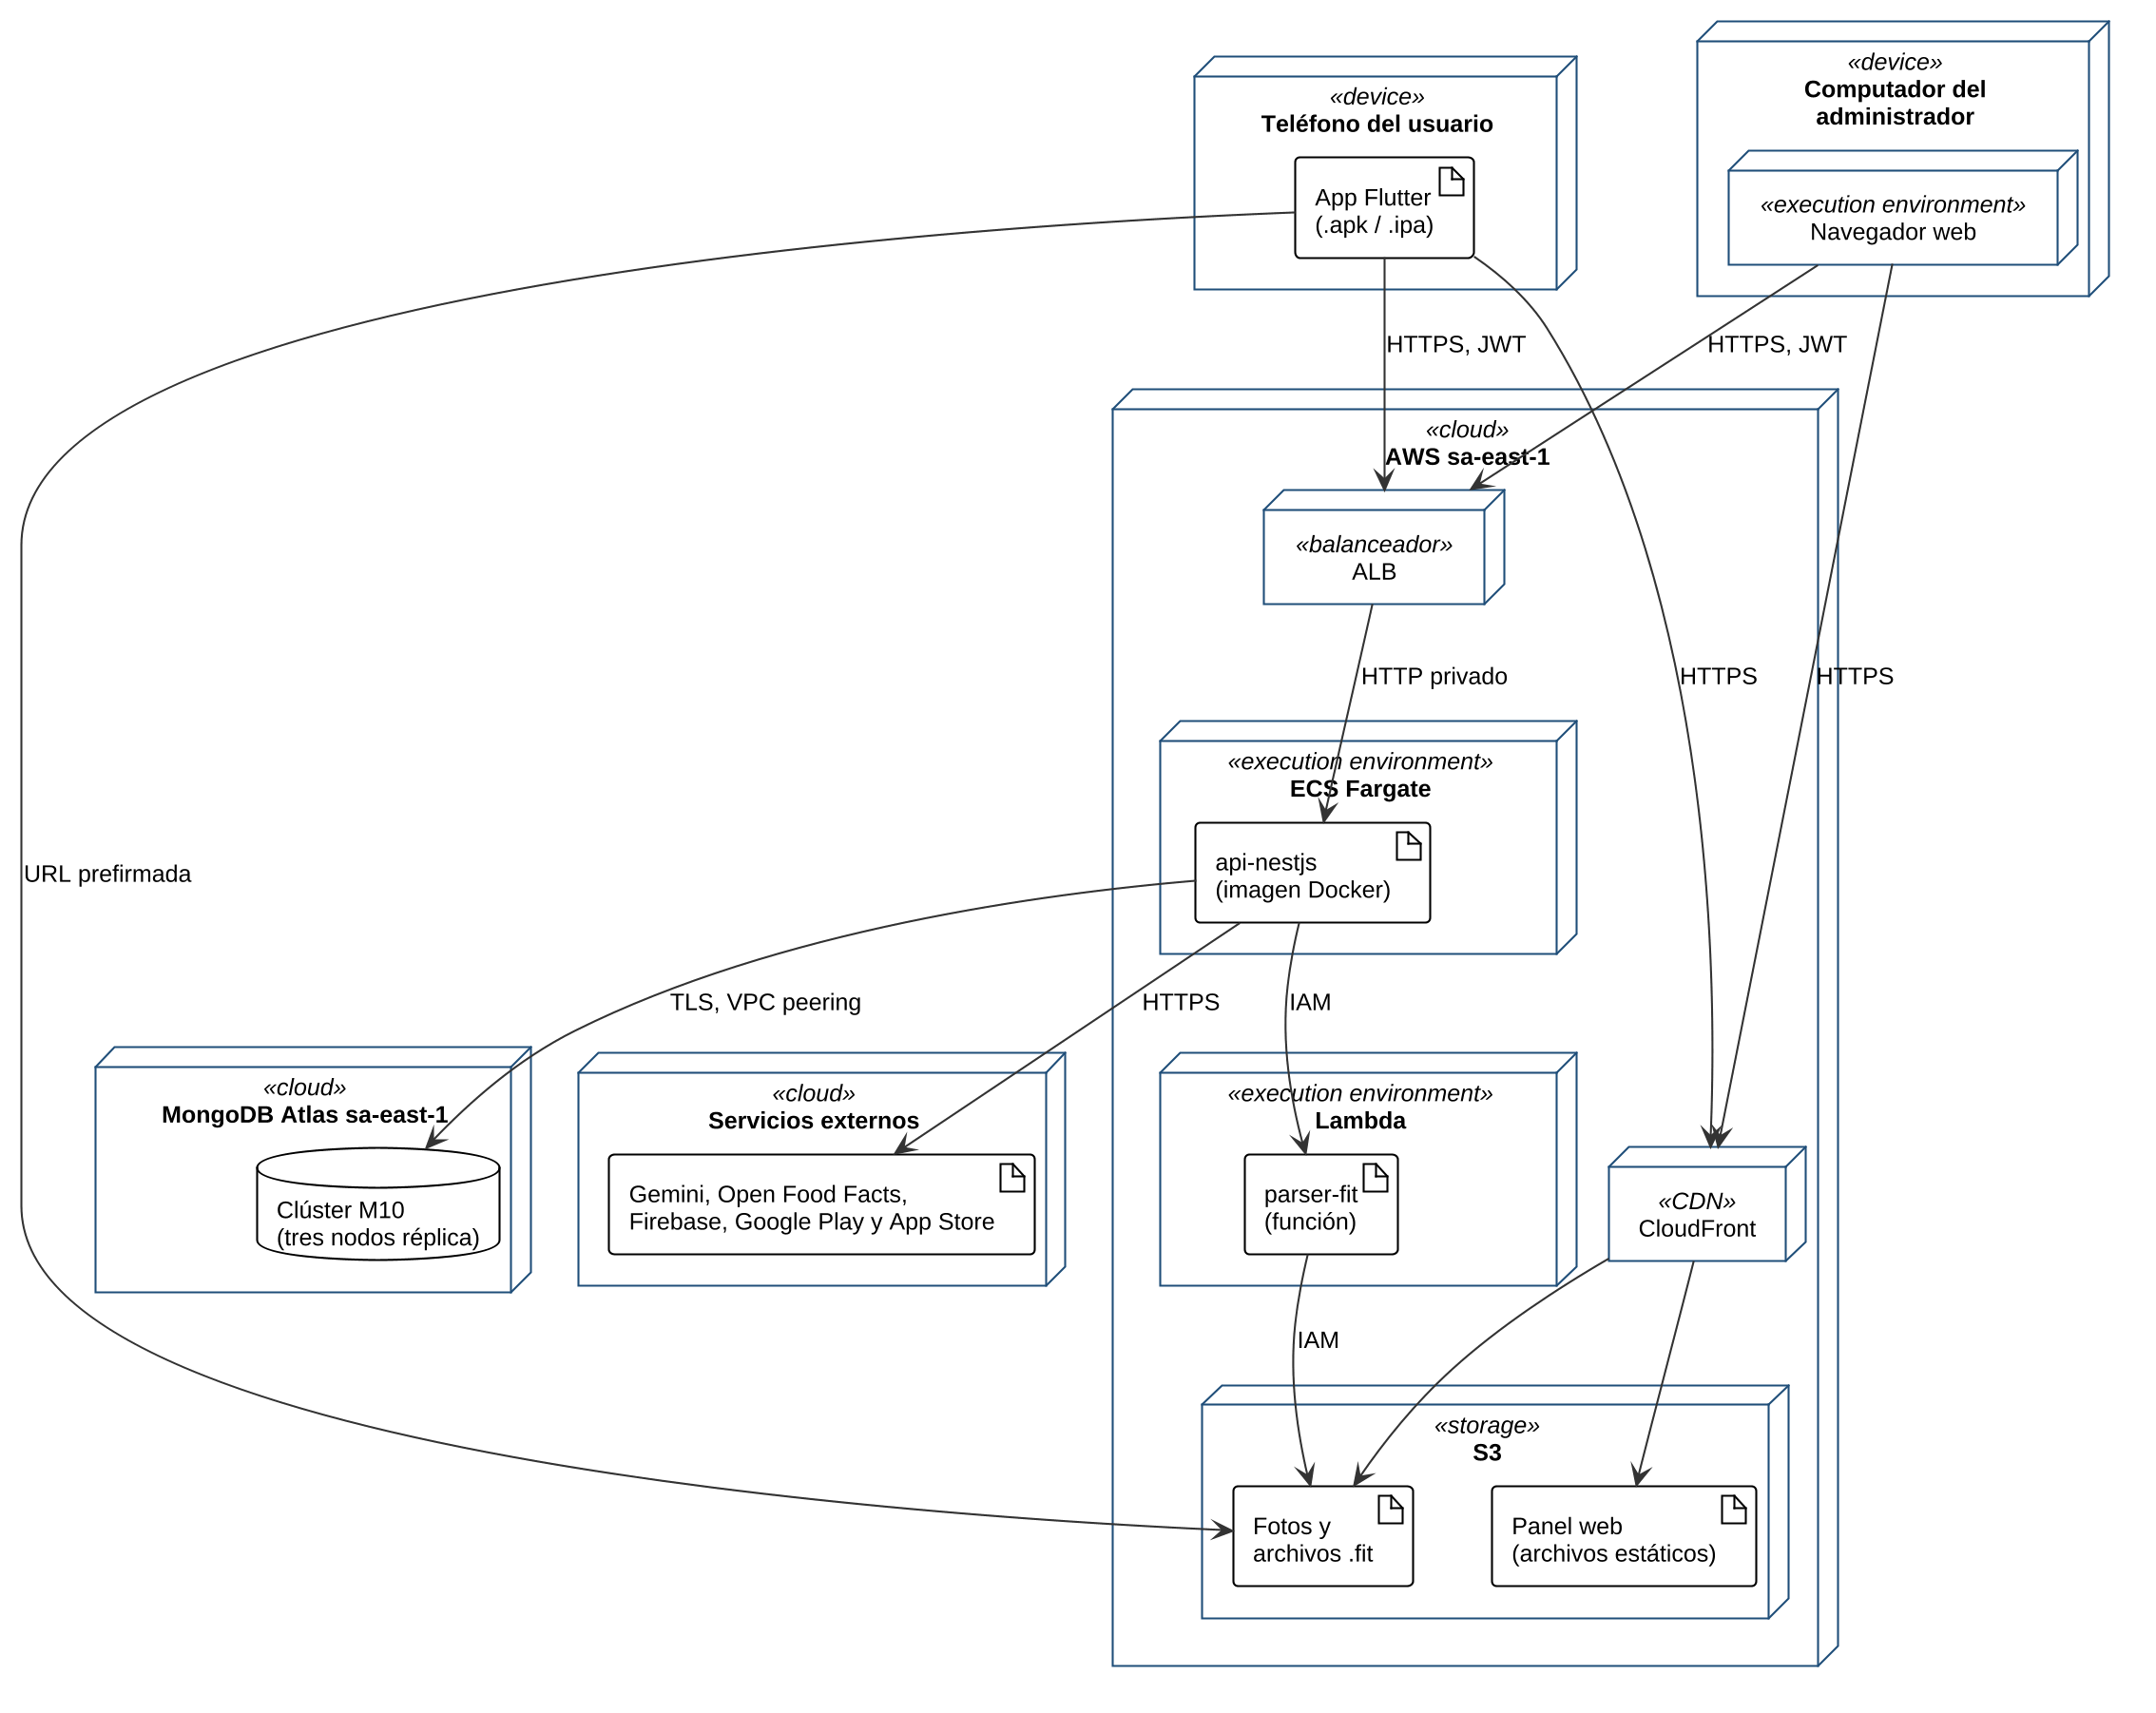
\includegraphics[width=0.9\textwidth,height=0.55\textheight,keepaspectratio]{figuras/arquitectura/diagrama_despliegue.png}
    \captionof{figure}{Diagrama de despliegue de la solución.}
    \label{fig:diagrama_despliegue}
\end{center}

El sistema se compone de cuatro piezas que se instalan por separado:

\begin{itemize}
    \item \textbf{Aplicación móvil:} Se compila desde un solo código en Flutter y se publica en Google Play (\texttt{.apk}) y en App Store (\texttt{.ipa}). Cada usuario la instala en su teléfono.
    \item \textbf{API:} Se empaqueta como una imagen Docker, que se guarda en Amazon ECR y se ejecuta en ECS Fargate. Para actualizarla, se inicia una tarea con la versión nueva y luego se apaga la anterior, de modo que el servicio no se interrumpe.
    \item \textbf{Parser \texttt{.fit}:} Se publica como una función de AWS Lambda. Solo la API puede invocarla, y solo tiene permiso para leer el bucket de archivos.
    \item \textbf{Panel web:} Son archivos estáticos que se guardan en S3 y se entregan a través de CloudFront. El administrador lo abre desde su navegador.
\end{itemize}

MongoDB Atlas lo opera su proveedor, por lo que no hay que instalar el motor de base de datos. Se debe crear el clúster, configurar la conexión privada con la red de AWS y definir los índices descritos en el modelo de datos. Las claves de los servicios externos se guardan en AWS Secrets Manager y no quedan en el código ni en la imagen Docker.
\begin{spacing}{1.0}
\subsection{Comentarios Generales del Capítulo}
En este capítulo se definió cómo se va a construir la solución. A partir de los requerimientos del capítulo anterior, se describió cada caso de uso con sus precondiciones, sus flujos y su diagrama de actividades, y se detalló su funcionamiento técnico con un diagrama de secuencia. También se diseñó el modelo de datos en MongoDB, las interfaces de usuario de cada caso de uso, las integraciones con los seis sistemas externos, la infraestructura y su despliegue.

\medskip
El diseño dejó dos aportes principales. El primero es que aclaró lo que faltaba. Al trazar cada caso de uso paso a paso, se encontraron datos necesarios que el modelo no tenía, como el registro de quién reporta una publicación, y se corrigieron antes de programar. El segundo es que se comprobaron los costos. Al dimensionar la infraestructura con precios reales de AWS en São Paulo, se vio que la estimación inicial era baja, lo que llevó a ajustar la factibilidad económica. Sumando el IVA, la comisión de las tiendas y el impuesto a la renta, la solución elegida necesita 159 suscriptores. También se tomaron decisiones para gastar solo en lo necesario, como usar una función Lambda para leer archivos \texttt{.fit} y subir las fotos directamente a Amazon S3, sin dejar de proteger los datos sensibles con una conexión privada a la base de datos.

\medskip
Algunos valores de este diseño todavía son supuestos que se deben confirmar, como la carga esperada, la compresión de los datos de telemetría y el precio de MongoDB Atlas en São Paulo. Esto es parte del prototipo evolutivo, ya que cada versión permitirá medir estos valores y ajustar el diseño. Lo mismo ocurre con las interfaces de usuario, ya que varias pantallas muestran por ahora datos simulados y se conectarán a medida que se implementen sus servicios. Con este capítulo quedan cumplidos los objetivos específicos 1 a 4, según los criterios de la Tabla \ref{tab:validacion}. El objetivo 5, que es implementar el MVP y verificar el cruce de datos, corresponde a la etapa siguiente. Para ello ya existe un prototipo funcional en iOS que implementa el registro de fuerza, el registro de cardio con GPS y la nutrición, además del cálculo de la carga y de la fatiga cruzada definido en el Capítulo 3, con pruebas unitarias. Con esta base, el proyecto puede avanzar a la implementación, donde se planifica la puesta en marcha y las pruebas del sistema.
\end{spacing}

\section{Bibliografía}
\begingroup
\sloppy
\emergencystretch=3em
\printbibliography[heading=none]
\endgroup
\end{document}